% !TEX root = ../geom_autistic_intro.tex
\section{Lie Theory I: Basics}

\subsection{Lie groups}

\begin{defn}[Topological group]
    A topological group is a group $G$ together with a topology on it that is compatible with the group structure. That is, both the inversion $g\mapsto g^{-1}$ and the multiplication $(g,h)\mapsto gh$ maps are continuous. This is equivalent to requiring that the map $G\times G\to G$ given by $(g,h)\mapsto gh^{-1}$ is continuous.
\end{defn}

Topological groups form a very big class and include things like ``infinite-dimensional Lie groups'', $p$-adic numbers, rational numbers, etc. It turns out that every locally compact and locally contractible topological group (in particular topological groups that are also topological manifolds) have a unique smooth structure compatible with the group structure, which is what a Lie group is. Hence we skip right to the definition of Lie groups, and for the most part will assume that they are smooth.

\begin{defn}[Lie group]
    A (real) Lie group is a group $G$ with a structure of a differentiable (or $C^k$-differentiable, $C^\infty$-smooth, $C^\omega$-analytic) manifold on it that is compatible with the group structure. That is, the map $G\times G\to G$ given by $(g,h)\mapsto gh^{-1}$ is differentiable (resp.~$C^k$, $C^\infty$, $C^\omega$). A complex Lie group is defined similarly, with both the manifold structure and the group structure being holomorphic (complex analytic).
\end{defn}

We will show that any twice differentiable Lie group has a unique compatible real analytic structure. In fact, one can show that differentiability is not required at all, and any topological manifold with a continuous group structure has a unique structure of an analytic Lie group. This is why most authors assume that Lie groups are smooth by definition.

\begin{prop}[{{\cite[Thm.~1.6.3]{DK}}}]
    Any twice-differentiable Lie group $G$ has a unique structure of a real analytic manifold which turns it into a real analytic Lie group, and such that the identity map on $G$ is a $C^2$-diffeomorphism between the two structures.
\end{prop}


\begin{defn}[Group translation and adjoint operators]
    The left and right translation operators on a group $G$ are defined by
    \[L_g(h)=gh,\quad R_g(h)=hg.\]
    
    The adjoint operator corresponding to an element $g\in G$ is
    \[\Adg_g h=L_g\circ R_g^{-1}(h)=ghg^{-1}.\]
\end{defn}


\begin{example}[Lie groups]
    \begin{enumerate}[label=(\alph*)]
        \item Let $\bbK=\bbR ,\mathbb{C}$, or $\bbH $ (quaternions, see below). Every $\bbK$-vector space $V$ is a Lie group with respect to its additive structure and the manifold structure of the real vector space obtained from $V$ by restriction of the algebraic structure. The dimension is $\dim_{\bbR }\bbK\cdot \dim V$.
        \item Every finite or countable group with discrete topology is a Lie group.
        \item The direct product $G\times H$ of two Lie groups $G,H$ is a Lie group with the product group structure and the differentiable structure of the product of manifolds.
        \item $\GL_n(\bbR )$ is the set of invertible $n\times n$ matrices with real entries. It is a group under matrix multiplication and an open subset of $\Mat_n(\bbR )\cong \bbR^{n^2}$. Matrix multiplication is obviously smooth and inversion is smooth by Cramer's rule.
        \item $\GL^+_n(\bbR )$, which is the subset of $\GL_n(\bbR )$ consisting of matrices with positive determinant. It is still a group and an open subset of $\GL_n(\bbR )$.
        \item If $H\subset G$ is an open subgroup (a subgroup that is an open subset) of a Lie group $G$, then $H$ is a Lie group with the inherited group and manifold structures.
        \item For any real or complex finite-dimensional vector space $V$, the group $\GL(V)$ of endomorphisms of $V$ is a Lie group.
        \item The unit circle $\bbS^1\subset \mathbb{C}^\ast$ with multiplication inherited from $\mathbb{C}$ is a Lie group.
        \item The $n$-torus $\bbT^n=\bbS^1\times\cdots\times \bbS^1$ is an $n$-dimensional abelian Lie group.
    \end{enumerate}
\end{example}

\begin{defn}[Lie group homomorphism]
    A Lie group homomorphism between two Lie groups $G,H$ is a smooth map $F:G\to H$ that is also a group homomorphism. If it is a diffeomorphism, it is called an isomorphism. These maps comprise the morphisms of the category $\mathsf{LieGr}$ of Lie groups.
\end{defn} 

\begin{example}[Lie group morphisms]
    \begin{enumerate}[label=(\alph*)]
        \item The inclusion map $\bbS^1\hookrightarrow \mathbb{C}^\ast$ is a Lie group homomorphism.
        \item The exponential map $\exp:(\bbR ,+)\to (\bbR_+,*)$ is a Lie group homomorphism since $\exp(x+y)=\exp(x)\cdot \exp(y)$.
        \item The determinant function $\det:\GL_n(\bbR )\to \bbR^\times$ is a Lie group homomorphism.
        \item The adjoint action $\Adg_g:G\to G$ is a Lie group homomorphism for any $g\in G$.
    \end{enumerate}
\end{example}

\begin{thm}[{{\cite[Thm.~7.5]{Lee}}}]
    Every Lie group homomorphism has constant rank.
\end{thm}
\begin{proof}
    Let $F:G\to H$ be a Lie group homomorphism. We will show that the differential $T_g F$ of $F$ at any $g\in G$ has the same rank as the differential $T_eF$ at the identity. We have
    \[F\circ L_g (h)=F(gh)=F(g)F(h)=L_{F(g)}\circ F(h),\]
    i.e.~$F\circ L_g=L_{F(g)}\circ F$. Computing the differential of both sides at the identity $e\in G$ using the chain rule, we find
    \[T_gF\circ T_e L_g=T_{F(g)}L_{F(g)}\circ T_e F.\]
    Left translation operators are diffeomorphisms and therefore both $T_e L_g$ and $T_{F(g)}L_{F(g)}$ are isomorphisms of tangent spaces. Compositions with isomorphisms don't change rank, therefore $\rank T_gF=\rank T_e F$ is constant on $G$.
\end{proof}
\begin{cor}[{{\cite[Cor.~5.3.7]{RS1}}}]\label{cor 5.3.7 RS1}
    For a Lie group homomorphism $\varphi:G\to H$, the following are equivalent:
    \begin{enumerate}
        \item $\varphi$ is an immersion (submersion).
        \item $\varphi$ has discrete kernel (is open).
        \item $\varphi_{\ast e}$ is injective (surjective).
    \end{enumerate}
    In addition, $\varphi$ is an isomorphism of Lie groups iff it is bijective.
\end{cor}
\begin{proof}
    Exercise $1\Rightarrow 2\Rightarrow 3 \Rightarrow 1$.
\end{proof}

The simplest nonabelian examples of compact Lie groups are the 3-dimensional rotation group and its ``complex form'', $\SU_2$. We now establish that $\SU_2$ is the universal covering space of $\SO_3(\bbR)$, and hence $\pi_1(\SO_3(\bbR))=\bbZ_2$. As we will show in the next section, every Lie group has a unique universal covering Lie group.

\begin{example}[$\SO_3(\bbR)$ and its double cover $\SU_2$]\label{example su2 and so3}
    The rotation group $\SO_3(\bbR)$ is known to be a Lie group because, for example, it can be parametrized by Euler angles as coordinates in a way that makes the group structure obviously smooth. We will have a general proof that orthogonal groups are Lie groups in Section~\ref{sec: classical groups}. This group can be alternatively parametrized by vectors $n\in\bbR^3$ as follows:
    \[R_n=I+\frac{\sin |n|}{|n|}A_n+\frac{1-\cos |n|}{|n|}A_n^2,\]
    where $|n|=\sqrt{n_1^2+n_2^2+n_3^2}$ is the rotation angle and 
    \[A_\omega=\begin{pmatrix}
        0&-\omega_3&\omega_2\\
        \omega_3&0&-\omega_1\\
        -\omega_2&\omega_1&0
    \end{pmatrix},\quad 
    A_\omega=\begin{pmatrix}
        -\omega_3^2-\omega_2^2 &\omega_1\omega_2 &\omega_3\omega_1\\
        \omega_1\omega_2& -\omega_3^2-\omega_1^2 & \omega_2\omega_3\\
        \omega_3\omega_1 & \omega_2\omega_3 & -\omega_1^2-\omega_2^2
    \end{pmatrix}
    .\]
    It is easy to check two important equalities 
    \[A_{\omega\times \xi}=A_\omega A_\xi-A_\xi A_\omega=[A_\omega,A_\xi],\quad \omega\cdot\xi=-\tr(A_\omega A_\xi).\label{eq R3->so(3) hom}\]
    If $|n|\in 2\pi\bbZ$, then $R_n$ is a rotation around the axis through $n$, through the angle $|n|$. Furthermore, if $0<|n|<\pi$, then $R_n$ is the unique rotation such that, for each nonzero vector $x\perp n$ in the plane of the rotation, the triple $(x,R_n\cdot x,n)$ has positive orientation, i.e.~$\det (x,R_n x,n)>0$. The mapping $n\mapsto R_n$ is surjective from the closed ball $|n|\leq \pi$ onto $\SO_3(\bbR)$, and a diffeomorphism from the open ball $|n|<\pi$ onto the dense subset of $\SO_3(\bbR)$ of rotations through an angle $<\pi$. Near the boundary sphere $S_\pi=\{n\in\bbR^3\mid |n|=\pi\}$, one can check that $n\mapsto R_n$ is a smooth two-fold covering map mapping $n$ and $(|n|-2\pi)\frac{n}{|n|}$ to the same element of $\SO_3(\bbR)$. In particular, $n\to R_n$ is a smooth two-fold covering from the sphere $S_\pi$ onto the subset of rotations through the angle $\pi$, mapping the antipodal points $\pm n$ to the same element of $\SO_3(\bbR)$. We thus see that $\SO_3(\bbR)$ is diffeomorphic to the real projective space $\RP^3$, which is the quotient of the closed ball $\bbD^3$ by the map that identifies antipodal boundary points, or equivalently the antipodal quotient of $\bbS^3$.
    
    The group $\SU_2$ is defined as the set of $2\times2$ complex matrices that preserve the standard Hermitian dot product $(z,w)^2=|z|^2+|w|^2$ on $\bbC^2$:
    \[\SU_2=\left\{g(a,b)=
    \begin{pmatrix}
        a&b\\-\wb{b}&\wb{a}
    \end{pmatrix}
    \middle| a,b\in\bbC, |a|^2+|b|^2=1
    \right\}.\]
    Clearly this is diffeomorphic to the unit sphere in $\bbC^2\cong \bbR^4$, i.e.~$\SU_2\cong \bbS^3$ as manifolds. One remarkable property is that 
    \[\bbR\cdot \SU_2=\left\{
    \begin{pmatrix}
        a&b\\-\wb{b}&\wb{a}
    \end{pmatrix}
    \middle| a,b\in\bbC
    \right\}\]
    is a 4-dimensional real-linear subspace of the (real 8-dimensional) space of complex $2\times 2$ matrices. This subspace is closed under matrix multiplication and in this way forms a noncommutative real division algebra. It has the famous quaternion basis consisting of the identity matrix $\bf{1}$ plus the three matrices
    \[\bf{i}=i\sigma_3=\begin{pmatrix}
        i&0\\0&-i
    \end{pmatrix},\quad 
    \bf{j}=i\sigma_2=\begin{pmatrix}
        0&1\\-1&0
    \end{pmatrix},\quad
    \bf{k}=i\sigma_1=\begin{pmatrix}
        0&i\\i&0
    \end{pmatrix}\]
    with relations $\bf{i}^2=\bf{j}^2=\bf{k}^2=\bf{ijk}=-\bf{1}$. So $\bbR\cdot\SU_2$ can be identified with the quaternion algebra $\bbH$ and $\SU_2$ is the multiplicative group of unit quaternions.
\end{example}










\subsection{Topology of Lie groups}

Recall that not every topological space has a universal covering space, and in particular not every topological group has one. However Lie groups are manifolds and therefore always have a universal covering manifold. We now show that the universal cover naturally becomes a Lie group itself.

\begin{thm}[Existence of a universal covering group {{\cite[Thm.~7.7]{Lee}}}]\label{thm 7.7. Lee covering group}
    Let $G$ be a connected Lie group. There exists a simply connected Lie group $\wt{G}$, called the \emph{universal covering group of $G$}, that admits a smooth covering map $\wt\pi:\wt{G}\to G$ that is also a Lie group homomorphism. This group is unique up to Lie group isomorphism.
\end{thm}
\begin{proof}
    Let $\wt G$ be the universal covering manifold of $G$ and $\wt\pi$ the corresponding smooth covering map. Then $\wt\pi\times\wt\pi:\wt G\times\wt G\to G\times G$ is also a smooth covering map.

    Let $m:G\times G\to G$ and $i:G\times G$ denote the multiplication and inversion maps of $G$, respectively, and let $\wt e$ be an arbitrary element of the fiber ${\wt\pi}^{-1}(e)\subset \wt{G}$. Since $\wt G$ is simply connected, the Lifting Theorem~\ref{Lifting Theorem} guarantees that the map $m\circ(\wt\pi\times\wt\pi):\wt G\times\wt G\to G$ has a unique continuous lifting $\wt m:\wt G\times\wt G\to \wt G$ satisfying $\wt m(\wt e,\wt e)=\wt e$ and $\wt\pi\circ \wt m=m\circ (\wt\pi\times\wt\pi)$:
    \[
    \begin{tikzcd}[every matrix/.append style={name=m}]
       \wt G\times \wt G \arrow[r,"\wt m"]\arrow[d,"\wt\pi\times\wt\pi",swap] & \wt G\arrow[d,"\wt\pi"]\\
       G\times G \arrow[r,"m", swap] & G.
    \end{tikzcd}
    \]
    Because $\wt\pi$ is a local diffeomorphism and $\wt\pi\circ \wt m=m\circ(\wt\pi\times\wt\pi)$ is smooth, it follows that $\wt m$ is smooth. By the same reasoning, $i\circ\wt\pi:\wt G\to G$ has a smooth lifting $\wt i:\wt G\to \wt G$ satisfying $\wt i(\wt e)=\wt e$ and $\wt\pi\circ \wt i=i\circ \wt\pi$:
    \[
    \begin{tikzcd}[every matrix/.append style={name=m}]
       \wt G \arrow[r,"\wt i"]\arrow[d,"\wt\pi",swap] & \wt G\arrow[d,"\wt\pi"]\\
       G \arrow[r,"i", swap] & G.
    \end{tikzcd}
    \]
    We define multiplication and inversion on $\wt G$ by $xy=\wt m(x,y)$ and $x^{-1}=\wt i(x)$. Then the diagrams above can be written as 
    \[\wt\pi(xy)=\wt\pi(x)\wt\pi(y),\quad \wt\pi(x^{-1})=\wt\pi(x)^{-1}.\label{47328}\]
    It remains only to show that $\wt G$ is a group with these operations, for then it is a Lie group because $\wt m$ and $\wt i$ are smooth, and then the last formula shows that $\wt\pi$ is a homomorphism. We leave the details, which can be found in \cite[Thm.~7.7]{Lee}, to the reader, since we will later provide another proof as a consequence of Theorem~\ref{thm 8.7 Sharpe}.

    % To show that $\wt{e}$ is an identity in $\wt G$, consider the map $f:\wt G\to \wt G$ defined by $f(x)=\wt e x$. Then $\wt\pi\circ f(x)=\wt\pi(\wt e)\wt\pi(x)=e\wt\pi(x)=\wt\pi(x)$, so $f$ is a lifting of $\wt\pi:\wt G\to G$. The identity map $\id_{\wt G}$ is another lifting of $\wt \pi$, and it agrees with $f$ at a point since $f(\wt e)=\wt m(\wt e,\wt e)=\wt e$, so the uniqueness of liftings (Lemma~\ref{lem 4.4 Bredon}) implies $f\equiv \id_{\wt G}$, or $\wt ex=x$. The same argument shows $x\wt e=x$.

    % Finally, we show that the multiplication $\wt m$ is associative. Consider two maps $\alpha_L,\alpha_R:(\wt G)^3\to \wt G$ defined by
    % \[\alpha_L(x,y,z)=(xy)z,\quad \alpha_R(x,y,z)=x(yz).\]
    % Then (\ref{47328}) implies that
    % \[\wt\pi\circ \alpha_L(x,y,z)=\left(\wt\pi(x)\wt\pi(y)\right)\wt\pi(z)=\wt\pi(x)\left(\wt\pi(y)\wt\pi(z)\right)=\wt\pi\circ\alpha_R(x,y,z),\]
    % so $\alpha_L$ and $\alpha_R$ are both liftings of the same map $\alpha(x,y,z)=\wt\pi(x)\wt\pi(y)\wt\pi(z)$. Since they agree at $(\wt e,\wt e,\wt e)$, they are equal. A similar argument shows that $x^{-1}x=xx^{-1}=\wt e$, so $\wt G$ is a group.
    
    Uniqueness follows from the uniqueness of covering spaces up to isomorphism and the fact that the only flexibility in the definition of the group structure is in the choice of the identity $\wt e$, but all such choices lead to isomorphic groups.
\end{proof}

\begin{cor}
    For a connected Lie group we have the exact sequence
    \[0\to \pi_1(G)\to \wt{G}\to G\to 0.\]
\end{cor}

\begin{example}[Universal covering groups]
    \begin{enumerate}[label=(\alph*)]
        \item $\bbR^n$ is the universal covering group of the torus $\bbT^n$.
        \item $\bbC$ is the universal covering group of $\bbC^\ast$ with the covering map $\exp:\bbC\to\bbC^\ast$.
    \end{enumerate}
\end{example}


\begin{prop}
    For any topological group $G$, the fundamental group $\pi_1(G)$ is abelian.
\end{prop}
\begin{proof}
    Fundamentally this follows from the fact that there are two different multiplication operations on loops in a group -- concatenation of loops, and multiplications of their values in the group. Specifically, given two loops $\gamma_1,\gamma_2$, a map $g(s,t)=\gamma_1(s)\gamma_2(t)$ provides a homotopy between $\gamma_1\bullet \gamma_2$ (along two sides of the square) and $\gamma_2\bullet\gamma_2$ (along the other two sides).
\end{proof}

We have already seen that $\pi_1(\SO_3(\bbR))=\bbZ_2$ by finding its universal covering group. Unfortunately, computing the fundamental groups of other classical groups is not so easy and will require considering the long exact sequences of certain fibrations, which will be easier to construct once we talk about group actions on manifolds. Another nontrivial fact from Lie theory will be that the fundamental group of any compact Lie group is finite, which means that the universal covering group of any compact Lie group is also compact.

First recall the following fundamental theorem that classifies all finitely generated abelian groups (it has nothing to do with the theory of Lie groups, so the proof can be skipped).

\begin{thm}[Classification of finitely generated abelian groups]\label{thm classification of finitely generated abelian gr}
    Every finitely generated abelian group is isomorphic to a group of the form
    \[\bbZ^n\oplus \bbZ_{k_1}\oplus \cdots\oplus \bbZ_{k_t}.\]
\end{thm}
\begin{proof}
    First we prove the following statement: if the abelian group $G$ is generated by a set $x_1,\ldots,x_k$, and $c_1,\ldots,c_k\in\bbN$ are such that $\gcd(c_1,\ldots,c_k)=1$, then there exists another set of generators $y_1,\ldots,y_k\in G$ such that $y_1=c_1x_1+\cdots c_kx_k$.

    We argue by induction on $s=c_1+\cdots+c_k$. The lemma certainly holds if $s=1$, and so we assume $s>1$. Then at least two $c_i$ are nonzero, say $c_1\geq c_2\geq 0$. Now
    \begin{itemize}
        \item $\{x_1,x_2+x_1,x_3,\ldots,x_k\}$ generates $G$,
        \item $\gcd(c_1-c_2,c_2,c_3,\ldots,c_k)=1$, and
        \item $(c_1-c_2)+c_2+\cdots+c_k<s$,
    \end{itemize}
    and so, by induction, there exist generators $y_1,\ldots, y_k$ for $G$ such that
    \[y_1=(c_1-c_2)x_1+c_2(x_1+x_2)+c_2x_3+\cdots c_kx_k=c_1x_1+\cdots +c_kx_k.\]

    Now we prove the classification theorem by induction on $k$. If $G$ can be generated by one element, the statement is trivial, so we ay assume that $k>1$. Among all generating sets $\{x_1,\ldots,x_k\}$ for $G$ with $k$ elements there is one for which the order of $x_1$ is the smallest possible. We shall show that $G$ is then the direct sum of $\<x_1\>$ and $\<x_2,\ldots,x_k\>$. This will complete the proof because the induction hypothesis provides us with a basis for the second group, which together with $x_1$ forms a basis for $G$.

    If $G$ is not the direct sum of $\<x_1\>$ and $\<x_2,\ldots,x_k\>$, then there exists a relation
    \[m_1x_1+m_2x_2+\cdots m_kx_k=0\]
    with $m_1x_1\neq 0$. After possibly changing the sign of some of the $x_i$, we may suppose that $m_1,\ldots,m_k\in\bbN$ and $m_1<\mathrm{ord}(x_1)$. Let $d=\gcd(m_1,\ldots,m_k)>0$ and let $c_i=m_i/d$. According to the first part of the proof, there exists a generating set $y_1,\ldots,y_k$ such that $y_1=c_1x_1+\cdots+c_kx_k$. But 
    \[dy_1=m_1x_1+\cdots m_kx_k=0\]
    and $d\leq m_1<\mathrm{ord}(x_1)$, and so this contradicts the choice of $\{x_1,\ldots,x_k\}$.
\end{proof}
\begin{rem}
    The \emph{torsion} subgroup of $G$ is defined as the subset of all elements of finite order:\index{Torsion subgroup}
    \[T(G)=\{x\in G:\;\exists m\in\bbN\; mx=0\},\]
    and then the theorem implies that each finitely generated abelian group has the form
    \[G\cong \bbZ^n\oplus T(G)\]
    where $T(G)$ is a finite abelian group.
    
    It is important to know that the power $n$ of $\bbZ$ is uniquely determined by $G$ and is called the \emph{rank} of $G$.\index{Rank of abelian group} Indeed, pick a prime $p$ not dividing any of the $k_i$'s and consider the quotient
    \[G\slash pG\cong (\bbZ\slash p\bbZ)^n,\]
    therefore $n$ is the dimension of $G\slash pG$ viewed as a vector space over the finite field $\bbF_p$, and thus depends only on $G$ itself.

    Furthermore, $k_i$'s can be chosen so that $k_1\geq 2$ and $k_1|n_2,\ldots, k_{t-1}|k_t$, and then they are also uniquely determined by $G$ (such $k_i$ are called \emph{invariant factors}\index{Invariant factors} of $G$). Alternatively, $k_i$'s can be chosen to be powers of prime numbers, which also determines them uniquely (such $k_i$ are called elementary divisors\index{Elementary divisors} of $G$). Both of these statements follow from the fact that if $\gcd(k,l)=1$ then $\bbZ_k\times \bbZ_l\cong \bbZ_{kl}$, which allows one to decompose the torsion part of $G$ into a product of cyclic groups of prime power orders.
\end{rem}


\begin{defn}[Centralizer]\index{Centralizer}
    Let $G$ be a group and $S\subset G$ a subset. The centralizer of $S$ is the subgroup
    \[\rmC_G(S)=\{g\in G\mid gsg^{-1}=s \text{ for all }s\in S\}.\]
    The center of $G$ is defined as $\rmZ(G)\coloneqq \rmC_G(G)$. If all elements of $S$ commute with each other, then $\rmC_G(S)$ is the largest subgroup of $G$ whose center contains $S$.
    
    The following properties hold. $G$ is abelian iff $\rmZ(G)=G$. A subgroup $H$ is abelian iff $H\subset \rmC_G(H)$. There is an inclusion $\rmC_G(S)\subset \rmN_G(S)$, and in fact $\rmC_G(S)$ is a normal subgroup of $N(S)$.
\end{defn}

\begin{prop}\label{prop discrete normal subgroup}
    Suppose $G$ is a connected topological group and $\Gamma\subset G$ is a discrete normal subgroup. Then $\Gamma\subset \rmZ(G)$.
\end{prop}
\begin{proof}
    Let $\gamma\in\Gamma$ and consider the continuous map $g\mapsto \Adg_g(\gamma)=g\gamma g^{-1}$ for $g\in G$. Since $\Gamma$ is normal, $\Adg_G(\gamma)\subset \Gamma$. Since $G$ is connected, the map is continuous, and $\Gamma$ is discrete, the image $\Adg_G(\gamma)$ must be a single point, and it must be $\gamma$ since we can choose $g=e$.
\end{proof}
This gives us yet another way of proving that $\pi_1(G)$ is always abelian.
\begin{cor}\label{cor G=wt G/Gamma}
    Every connected Lie group $G$ has the form $\wt{G}\slash\Gamma$, where $\wt{G}$ is simply connected and $\Gamma\cong \pi_1(G)$ is a discrete subgroup of the center $\rmZ(\wt{G})$. In particular, $\pi_1(G)$ is abelian.
\end{cor}
\begin{cor}[Classification of discrete subgroups of $\bbR^n$]\label{cor discrete subgroups of Rn}
    % If $G$ is an abelian Lie group, then $G$ is of the form $\bbR^n\slash\Gamma$, where $\Gamma$ is a discrete subgroup of $\bbR^n$. As a consequence, $G\cong (S^1)^k\times \bbR^{n-k}$.
    Any discrete subgroup $\Gamma$ of $\bbR^n$ is a free abelian subgroup, i.e.~a lattice generated by a set of linearly independent vectors $x_1\ldots,x_k$.
\end{cor}
\begin{proof}
    Indeed, consider the subspace $V\subset \bbR^n$ spanned by $\Gamma$. Let its dimension be $k$ and let $v_1,\ldots,v_k\in \Gamma$ be a set of elements of $\Gamma$ that forms a basis for $V$, and let $Z=\{\bbZ v_1+\cdots +\bbZ v_k\cong \bbZ^k\}\cong\bbZ^k$. Consider the quotient map $q:V\to V/Z$ (this is a quotient by a subgroup, not just a topological quotient: its fibers are $q^{-1}(v)=v+Z$). It is open and the quotient space is compact (being homeomorphic to a torus $\bbT^k$). The fact that $\Gamma$ is discrete and $q$-saturated (i.e.~$q^{-1}(q(\Gamma))=\Gamma$) implies that $q(\Gamma)$ is discrete. 
    
    Moreover, $\Gamma$ is closed because otherwise there would exist a Cauchy sequence $(\gamma_k)\in\Gamma$, i.e.~$\gamma_k-\gamma_{k+1}\to 0$ (the existence of a limit is irrelevant for this proof, a mere existence of a Cauchy sequence is enough), which would contradict the fact that $0$ is isolated in $\Gamma$. Therefore, by definition of the quotient topology and since $\Gamma$ is $q$-saturated, $q(\Gamma)$ is also closed.  Therefore $q(\Gamma)\cong \Gamma\slash \bbZ^k$ is compact and discrete, hence finite. Since $\bbZ^k$ and $\Gamma\slash \bbZ^k$ are both finitely generated, it follows that $\Gamma$ is also finitely generated (by the union of the generators of $\bbZ^k$ and $\Gamma\slash \bbZ^k$). Since $V$ is torsion-free, we obtain that $\Gamma$ is free abelian.  The fact that $\Gamma\slash \bbZ^k$ is finite then implies that $\rank \Gamma=k$. Therefore there exists a set of generators $x_1,\ldots,x_k$ for $\Gamma$ which also provide a basis for $V$.
    % In summary, $G$ is the quotient of its universal covering group, which must be abelian and simply connected, hence isomorphic to $\bbR^n$, by a discrete subgroup. As we just showed, this produces a decomposition $\bbR^n\slash\Gamma \cong (\bbR^k\slash\Gamma) \oplus \bbR^{n-k}\cong \bbT^k\oplus \bbR^{n-k}$.
\end{proof}
\begin{rem}
    We will later show that $\bbR^n$ are the only simply connected abelian Lie groups, and it will follow that any other connected abelian Lie group $G$ is a quotient of $\bbR^n$ by a lattice of rank $k\leq n$, so $G\cong \bbT^k\oplus \bbR^{n-k}$.
    
    This gives us another way of proving the Fundamental Theorem of Algebra. If $\bbF/\bbR$ is a field extension, then the identity component $(\bbF^\ast)_0$ is abelian and connected. Then for extension of degree $d=1$, this is $\bbR$; for $d=2$ this is $\bbS^1\times\bbR\cong\bbC^\ast$, and for $d\geq 3$ this is $\bbS^{d-1}\times\bbR$, but none of these can be abelian Lie groups. Hence $\bbC$ is the largest extension of $\bbR$ and hence algebraically closed.
\end{rem}





\subsection{Lie subgroups}

\begin{defn}[Lie subgroup]
    A Lie subgroup $H$ of a Lie group $G$ is an immersed submanifold such that the induced group structure turns it into a Lie group. In particular, the inclusion map $i:H\hookrightarrow G$ is a smooth immersion and a Lie group homomorphism.
\end{defn}

Note that Lie subgroups are not generally required to be embedded submanifolds. For example, the dense immersion of $\bbR$ into the torus $\bbT^2$ (as a straight line with an irrational slope) is a Lie homomorphism. We will show later that its image is a Lie subgroup.

\begin{prop}[{{\cite[Prop.~7.11]{Lee}}}]\label{prop 7.11 Lee}
    Let $G$ be a Lie group, and suppose $H\subset G$ is a subgroup that is also an embedded submanifold. Then $H$ is a Lie subgroup.
\end{prop}
\begin{proof}
    We only need to check that the multiplication and inversion maps on $H$ are smooth. Both of them are restrictions of smooth maps either $G\times G\to G$ or $G\to G$ to $H\times H\to G$ and $H\to G$, and are therefore smooth. Since $H$ is an embedded submanifold, restricting the codomain of a smooth map into $G$ to $H$ also produces a smooth map by Theorem~\ref{thm 5.27 Lee}.
\end{proof}

\begin{lem}[{{\cite[Lem.~7.12]{Lee}}}]\label{lem 7.12 Lee}
    Let $H\subset G$ be an open subgroup of the Lie group $G$. Then $H$ is an embedded Lie subgroup. In addition, $H$ is closed, so it is a union of connected components of $G$.
\end{lem}
\begin{proof}
    Any open subset is an embedded submanifold. Every left coset $gH$ is open in $G$ since it is an image of an open subset under the diffeomorphism $L_g$. Since the complement $G\setminus H$ is the union of the cosets of $H$ other than $H$, it is open, and therefore $H$ is closed.
\end{proof}

The following is a simple exercise.
\begin{prop}[{{\cite[Prop.~7.15]{Lee}}}]
    Let $G$ be a Lie group and let $G_0$ be the connected component of the identity $e\in G$. Then $G_0$ is a normal subgroup of $G$, and is the only connected open subgroup. Every connected component of $G$ is diffeomorphic to $G_0$.
\end{prop}

\begin{defn}[Identity component]
    The identity component of a Lie group $G$ is the connected component $G_0$ of the identity $e\in G$.
\end{defn}

\begin{prop}[{{\cite[Prop.~7.14]{Lee}}}]\label{prop 7.14 Lee}
    The identity component $G_0\subset G$ is generated by any connected open neighborhood $U$ of $e\in G$ (i.e.~it is the smallest subgroup containing $U$).
\end{prop}
\begin{proof}
    Let $H$ be the subgroup generated by $U$. \gls{wlog}, we can take $U$ to be a symmetric neighborhood of the identity, i.e.~$U^{-1}=U$ (otherwise simply replace it with $U\cap U^{-1}$, which is also open). Let $U^k$ be the set of all elements of $G$ that can be expressed as a product of $k$ elements of $U$. Then $H=\bigcup_{k=1}^\infty U^k$ (this is a simple exercise). Since multiplication is a diffeomorphism, each $U^k$ can be written as a union of open sets, and thus $H$ is open.

    Since $U$ is connected and multiplication is continuous, each $U^k$ is connected. Thus $H$ is also connected by virtue of being a union of overlapping (at $e$) connected sets.

    By Lemma~\ref{lem 7.12 Lee}, $H$ must be the identity component.
\end{proof}


\begin{prop}[{{\cite[Prop.~7.16]{Lee}}}]
    Let $F:G\to H$ be a Lie group homomorphism. Then $\ker F$ is a properly embedded Lie subgroup of $G$ of codimension $\rank F$.
\end{prop}
\begin{proof}
    Because $F$ has constant rank, its kernel $F^{-1}(e)$ is a properly embedded submanifold of codimension equal to $\rank F$ by Theorem~\ref{thm level set submanifold}. It is thus a Lie subgroup by Proposition~\ref{prop 7.11 Lee}.
\end{proof}

\begin{prop}[{{\cite[Prop.~7.17]{Lee}}}]
    If $F:G\to H$ is an injective Lie group homomorphism, the image of $F$ has a unique smooth manifold structure such that $F(G)$ is a Lie subgroup of $H$ and $F:G\to F(G)$ is a Lie group isomorphism.
\end{prop}
\begin{proof}
    Since a Lie group homomorphism has constant rank, it follows by the Global Rank Theorem~\ref{Global rank} that $F$ is a smooth immersion. Proposition~\ref{prop 5.18 Lee} shows that $F(G)$ has a unique smooth structure such that it is an immersed submanifold of $H$ and $F$ is a diffeomorphism onto its image. It is a Lie group (because $G$ is), and it is a subgroup for algebraic reasons, therefore it is a Lie subgroup. Because $F:G\to F(G)$ is a group isomorphism and a diffeomorphism, it is a Lie group isomorphism.
\end{proof}
\begin{rem}
    As we will show later, a similar theorem holds for the image of \emph{any} Lie group homomorphism, not just injective.
\end{rem}

\begin{example}[Dense Lie subgroup of the torus]
    Let $H\subset \bbT^2$ be the dense submanifold of the torus that is the image of the immersion $\gamma:\bbR\to\bbT^2$ defining a straight line with an irrational slope. It is easy to check that $\gamma$ is an injective Lie group homomorphism, and thus $H$ is an immersed Lie subgroup of $\bbT^2$. Note that $\gamma(\bbR)$ is neither an open nor a closed subgroup of $\bbT^2$. Indeed, as we will show in the Closed Subgroup Theorem, any closed subgroup of a Lie group has to be an embedded Lie subgroup.
\end{example}

\begin{example}[Embedded Lie Subgroups]
    \begin{enumerate}[label=(\alph*)]
        \item $\SL_n(\bbR)$ is the kernel of the determinant homomorphism $\det:\GL_n(\bbR)\to \bbR^\times$, and is therefore a properly embedded Lie subgroup. Since $\det$ is surjective, it is a smooth submersion by the global rank theorem, so $\SL_n(\bbR)$ has dimension $n^2-1$.
        \item Similarly $\SL_n(\bbC)$ is a properly embedded Lie subgroup of $\GL_n(\bbC)$ of real dimension $2n^2-2$.
    \end{enumerate}
\end{example}

Typically we will be interested in closed subgroups, and the following result is a very important property.

\begin{thm}[{{\cite[Thm.~7.21]{Lee}}}]\label{thm 7.21 Lee}
    A Lie subgroup of a Lie group is closed iff it is embedded.
\end{thm}

We skip the proof of this theorem since later on we will derive a much stronger version of it, the Closed Subgroup Theorem~\ref{thm closed subgroup}, which asserts that \emph{every} closed subgroup (not necessarily a submanifold!) of a Lie group is automatically embedded.









\subsection{Classical Lie groups}\label{sec: classical groups}


\begin{example}[Classical groups]
    Let $\bbK=\bbR,\bbC,\bbH$. For $n,m=0,1,2\ldots$, define
    \[\rmI_{n,m}=
    \begin{bmatrix}
        \rmI_n&0\\0&-\rmI_m
    \end{bmatrix},\quad \rmJ_n=
    \begin{bmatrix}
        0&\rmI_n\\-\rmI_n&0
    \end{bmatrix}.
    \]
    A classical Lie group can be most generally defined as the subgroup of $\GL(\bbK^n)$ consisting of transformations that preserve some nondegenerate bilinear or sesquilinear form $B:\bbK^2\to \bbK$. However, there are no nontrivial bilinear forms over $\bbH$, and only $\bbR$ admits symmetric bilinear forms with a signature (which isn't all pluses). Hermitian forms have basis-independent signature in both the complex and the quaternionic case (the real case reduces to the symmetric one). A skew-Hermitian form on a complex vector space is rendered Hermitian by multiplication by $i$, so in this case, only $\bbH$ is interesting. Thus, with some work, one can show that any classical Lie group is isomorphic to one of the groups we define here (the \href{https://en.wikipedia.org/wiki/Classical_group}{Wikipedia page} has a full derivation).
    \begin{enumerate}
        \item Real and complex unimodular groups
        \[\SL_n(\bbK)=\{a\in\GL_n(\bbK)\mid \det a=1\}, \bbK=\bbR,\bbC.\]
        \item The real orthogonal group
        \[\Or_{n,m}=\{a\in\GL_{n+m}(\bbR)\mid a^T \rmI_{n,m}a=\rmI_{n,m}\}.\]
        In the case $m=0$ we write $\Or_n$ or $\Or_n(\bbR)$ for the group of linear isometries of the Euclidean scalar product.

        The special orthogonal group is the subgroup of $\Or_{n,m}$ of isometries that preserve orientation, i.e.~the unimodular ones
        \[\SO_{n,m}=\Or_{n,m}\cap \SL_{n+m}(\bbR).\]
        In the case $m=0$ we write $\SO_n$ or $\SO_n(\bbR)$.
        \item The complex orthogonal group
        \[\Or_{n}(\bbC)=\{a\in\GL_{n}(\bbC)\mid a^T a=\rmI_{n}\}.\]

        The special complex orthogonal group is the subgroup of $\Or_{n}(\bbC)$ of unimodular isometries
        \[\SO_{n}(\bbC)=\Or_{n}(\bbC)\cap \SL_{n}(\bbC).\]
        \item The unitary group
        \[\U_{n,m}=\{a\in \GL(n+m,\bbC)\mid a^\dagger \rmI_{n,m}a=\rmI_{n,m}\}.\]
        In the case $m=0$ we write $\U_n$ for the group of linear isometries of the standard Hermitian scalar product on $\bbC^n$.

        The special unitary group is the subgroup of unimodular unitary transformations
        \[\SU_{n,m}=\U_{n,m}\cap \SL_{n+m}(\bbC).\]
        In the case $m=0$ we write $\SU_n$.
        \item The symplectic group is the group of isometries of the antisymmetric bilinear form $\omega(x,y)=(x,\rmJ_n y)$ on $\bbK^{2n}$,
        \[\Sp_n(\bbK)=\{a\in\GL_{2n}(\bbK)\mid a^T \rmJ_n a=\rmJ_n\}.\]
        \item The quaternionic symplectic group is the group of isometries of the Hermitian form $(\wb{x},\rmI_{n,m}y)$ on $\bbH^{n+m}$,
        \[\Sp_{n,m}=\{a\in\GL_{n,m}(\bbH)\mid a^\dagger \rmI_{n,m}a=\rmI_{n,m}\}.\]
        In the case $m=0$ we write $\Sp_n$ for the group of linear isometries of the standard scalar product on $\bbH^n$. Note that these groups are in fact different from their complex and real versions. The difference is explained in detail in \cite[pp.~5-6]{Sepanski}.
    \end{enumerate}
\end{example}

Since we already know that $\GL_n(\bbK)$ is a smooth manifold, we can use the Level Set Theorem~\ref{thm level set submanifold} to conclude that all of these classical groups are also smooth properly embedded manifolds. The multiplication and inversion operations on them are smooth by virtue of being the restrictions of the ones on $\GL_n(\bbK)$ and hence these groups are Lie groups. The groups $\Or_n$, $\U_n$, and $\Sp_n$ also turn out to be compact because, for example, all of their elements have bounded matrix norms (e.g.~real orthogonal matrices of size $n\times n$ have matrix norm $\sqrt{n}$).


\begin{example}[$\SU_2\cong \Sp_1$]
    Recall that the quaternion algebra $\bbH$ is isomorphic to the algebra of $2\times 2$ complex matrices, $\Mat_2(\bbC)$:
    \[a_0 bf{1}+a_1 \bf{i}+a_2 \bf{j}+a_3 \bf{k}\mapsto
    \begin{pmatrix}
        a_0+\i a_1&a_2+\i a_3\\
        -a_2+\i a_3&a_0-\i a_1
    \end{pmatrix}, \; a_0,a_1,a_2,a_3\in\bbR.\label{46939}
    \]
    It is easy to check that the image of $\Sp_1$ under this homomorphism coincides with $\SU_2$. Hence, by restriction in range, it induces a group isomorphism from $\Sp_1$ onto $\SU_2$ which is smooth in both directions and hence a Lie group isomorphism.
\end{example}

\begin{example}[Universal coverings of $\SO_3$ and $\SO_4$]\label{example universal covering groups of so3 and so4}
    Identify $\bbR^4$ with $\bbH$ by the isometric isomorphism of real vector spaces
    \[\lambda(\bf{x})=x_0\bf{1}+x_1 \bf{i}+x_2 \bf{j}+x_3 \bf{k}.\]
    Every pair of quaternions $(\bf{a},\bf{b})$ defines a real-linear mapping $\bbH\to \bbH$ by $q\mapsto \bf{a}q\wb{\bf{b}}$ (where $\wb{\bf{b}}=b_0 \bf{1}-b_1\bf{i}-b_2\bf{j}-b_3\bf{k}$) and hence a linear mapping $\phi(\bf{a},\bf{b})$ of $\bbR^4$ by
    \[\phi(\bf{a},\bf{b})x=\lambda^{-1}\left(\bf{a}\lambda(x)\wb{\bf{b}}\right),\quad x\in\bbR^4.\label{10423}\]
    By assigning $\phi(\bf{a},\bf{b})$ to $(\bf{a},\bf{b})$ one obtains a map $\bbH\oplus\bbH\to \Mat_4(\bbR)$. This is a homomorphism of real algebras, and in particular it is smooth.

    First consider $\phi(\bf{a},\bf{a})$ for $a\in\Sp_1$. Due to $\lVert \bf{a}\rVert^2=1$, $\phi(\bf{a},\bf{a})$ is orthogonal. Since it leaves invariant the subspace $\bbR\times\{0\}\subset\bbR^4$, it also leaves invariant the subspace $\{0\}\times\bbR^3\subset\bbR^4$. Hence, restriction of $\phi$ in domain to the submanifold $\{(\bf{a},\bf{a})\mid \bf{a}\in\Sp_1\}$ of $\bbH\oplus\bbH$ and in range to the embedded submanifold of $\Mat_4(\bbR)$ consisting of the matrices
    \[\begin{bmatrix}
        1&0\\0&R
    \end{bmatrix},\quad R\in\Or_3,\]
    yields a Lie group homomorphism $\phi:\Sp_1\to \Or_3$. The defining equation reduces to
    \[\phi(\bf{a})x=\lambda^{-1}\left(\bf{a}(x_1\bf{i}+x_2\bf{j}+x_3\bf{k})\wb{\bf{a}}\right),\quad x\in\bbR^3.\label{10424}\]
    For $\bf{a}\in\bbH$, an explicit calculation yields
    \[[\phi(\bf{a})]_{ij}=(a_0^2-a_1^2-a_2^2-a_3^2)\delta_{ij}+2(a_i a_j-a_0\epsilon_{ijk}a_k).\]
    We determine the kernel and the image of $\phi$. According to (\ref{10424}), $\bf{a}\in\ker\phi$ iff $\bf{a}$ commutes with all quaternions. Then $\bf{a}=a\bf{1}$, $a\in\bbR$, hence $\ker\phi=\{\pm \bf{1}\}$, the center of $\Sp_1$. To find $\im\phi$, one first shows that $\phi$ is an immersion (exercise). Then, since $\Sp_1$ and $\SO_3$ have the same dimension, $\phi$ is a submersion and hence an open mapping by Proposition~\ref{thm submersions are open quotient maps}. It follows that $\im\phi$ contains a neighborhood of the identity $I\in\SO_3$. Since $\im\phi$ is a subgroup, by Proposition~\ref{prop 7.14 Lee}, it contains the identity component $\SO_3$ of $\Or_3$. Since $\Sp_1$ is connected, we finally obtain $\im\phi=\SO_3$.

    Since $\Sp_1$ coincides with the unit sphere in $\bbH$ and since $\ker\phi=\{\pm\bf{1}\}$ implies that the preimage of a point in $\SO_3$ under $\phi$ consists of antipodal points, $\phi$ induces a bijection $\RP^3\cong \SO_3$. Since both $\phi$ and the projection $\bbS^3\to\RP^3$ are submersions, this bijection is in fact a diffeomorphism.

    Next, consider $\phi(\bf{a},\bf{b})$ for $\bf{a},\bf{b}\in\Sp_1$. Due to $\lVert \bf{a}\rVert^2=\lVert \bf{b}\rVert^2=1$, $\phi(\bf{a},\bf{b})$ is orthogonal. Hence, by restriction in domain and range, $\phi$ induces a Lie group homomorphism $\phi:\Sp_1\times\Sp_1\to \Or_4$ with the defining equation (\ref{10423}). Arguing as before one finds $\ker\phi=\{\pm(\bf{1},\bf{1})\}$ and $\im\phi=\SO_4$. In particular, we conclude that there is a homeomorphism $\SO_4\cong \bbS^3\times \SO_3$.

    Let us add that via the algebra homomorphism (\ref{46939}), all of the above has an equivalent formulation in terms of complex $2\times 2$ matrices. This formulation is obtained by replacing $\Sp_1$ by $\SU_2$, $\bbH$ by the real vector space spanned by $\rmI_2$ and the traceless skew-Hermitian matrices, equipped with the scalar product $(A,B)=\tr(A^\dagger B)$, and the subspace of $\bbH$ spanned by $\bf{i},\bf{j},\bf{k})$ by the subspace of traceless skew-Hermitian matrices. This exactly recovers our previous construction of $\SU_2$ as a double cover of $\SO_3(\bbR)$.
\end{example}

\begin{rem}
    Using octonions one can construct in the same way a homeomorphism $\SO_8\cong \bbS^7\times \SO_7$. But in all other cases $\SO_n$ is only a `twisted product' of $\SO_{n-1}$ and $\bbS^{n-1}$, see \cite[Cor.~4D.3]{Hatcher}.
\end{rem}




\begin{example}[Universal covering of $\SO^+_{1,3}$]\label{example so13 and sl2c}
    Let $S_2(\bbC)$ be the 4-dimensional real vector space of $2\times 2$ complex Hermitian matrices parametrized by the mapping
    \[\lambda:\bbR^4\to S_2(\bbC),\quad \lambda(x)=
    \begin{pmatrix}
        x_0+x_1&-\i x_2+x_3\\
        \i x_2+x_3&x_0-x_1
    \end{pmatrix}.
    \]
    It is isometric with respect to the quadratic forms $x_0^2-x_1^2-x_2^2-x_3^2$ on $\bbR^4$ and $A\mapsto \det A$ on $S_2(\bbC)$. For every $a\in\Mat_2(\bbC)$, the assignment $A\mapsto aAa^\dagger$ defines a linear mapping of $S_2(\bbC)$ and hence a linear mapping $\phi(a)$ of $\bbR^4$ given by
    \[\phi(a)x=\lambda^{-1}\left(a\lambda(x)a^\dagger\right).\]
    The assignment $a\mapsto \phi(a)$, in turn, defines a map $\phi:\Mat_2(\bbC)\to \Mat_4(\bbR)$. This map is real homogenous of degree 2, hence smppth, and satisfies $\phi(ab)=\phi(a)\phi(b)$. Since for every $a\in\SL_2(\bbC)$ we have $\det aAa^\dagger =\det A$, $\phi$ restricts to a Lie group homomorphism $\phi:\SL_2(\bbC)\to \Or_{1,3}$. By similar arguments as in the last example, one finds $\ker\phi=\{\pm \rmI\}$ (which is the center of $\SL_2(\bbC)$), $\im\phi=\SO^+_{1,3}$ (the identity component of $\SO_{1,3}$, which is the \emph{proper orthochronous Lorentz group} that preserves both spatial and temporal orientations) and that $\phi$ is a covering homomorphism. It is a universal covering because $\SL_2(\bbC)$ is simply connected. To see this, one may use the polar decomposition which yields a diffeomorphism $\U_2\times S_2(\bbC)\to \GL_2(\bbC)$, given by $(a,A)\mapsto a\rme^A$. Restriction of this diffeomorphism to the submanifold $\SU_2$ of $\U_2$ times the subspace of traceless elements of $S_2(\bbC)$ induces a diffeomorphism $\bbS^3\times \bbR^3\to \SL_2(\bbC)$. Hence, $\phi$ is the universal covering homomorphism and $\SL_2(\bbC)$ is the universal covering group of $\SO^+_{1,3}$.
\end{example}

As we have just discovered, the universal covering group of $\SO_3$ is $\SU_2\cong\Sp_1$. It is also called the spin group $\Spin_3$. However, not every universal covering group of a classical group is a classical group itself. The higher-dimensional spin groups, for instance, are not isomorphic to classical groups except for a few ``accidental isomorphisms''.

\begin{defn}[Pin and Spin groups]\index{Spin groups}\index{Pin groups}
    For $n\geq 3$, the universal covering group of  $\Or_n$ is called $\Pin_n$, and that of $\SO_n$ is called $\Spin_n$.
\end{defn}

We note that this is not the ``proper'' definition of spin groups, which is actually a larger class that also includes $\Pin_{n,m},\Spin_{n,m}$, and their complex versions, none of which are generally simply connected and hence are not universal covers of any classical groups.

\begin{prop}
    The following deformation retracts exist:
    \begin{gather}
        \GL_n(\bbR)\to \Or_n(\bbR),\quad \GL_n(\bbC)\to \U_n, \quad \GL_n(\bbH)\to \Sp_n,\\
        \SL_n(\bbR)\to \SO_n(\bbR),\quad \SL_n(\bbC)\to \SU_n.
    \end{gather}
\end{prop}
\begin{proof}
     This is done by Gram-Schmidt orthonormalization and its complex and quaternionic analogs. To any ordered basis $(v_1,v_2,\ldots,v_n)$ of the space $V=\bbK^n$ associate the ``flag'' of subspaces $V_0=\{0\}$, $V_1=\langle v_1\rangle$, $V_2=\langle v_1,v_2\rangle$, and so on until $V_n=V$. The Gram-Schmidt algorithm turns any such basis into an orthonormal basis $(b_1,\ldots,b_n)$ that gives rise to the same flag of subspaces. It is moreover the unique such basis (orthonormal and with this same flag) for which in addition each $b_i$, inside $V_i$, is on the same side of the hyperplane $V_{i-1}$ as the original basis vector $v_i$.

     Now taking $V=\bbR^n$ we can identify $\GL_n^+(\bbR)$ (the identity component of $\GL_n(\bbR)$) with the set of ordered bases $\bf{v}=(v_1,\ldots,v_n)$  with $\det \bf{v}>0$, and $\SO_n(\bbR)$ with the set of orthonormal bases $\bf{b}$ with $\det \bf{b}=1$. Now for such a basis $\bf{v}$ let $\bf{b}$ be the corresponding Gram-Schmidt orthonormal basis, and simultaneously (or successively) deform every $v_i$ linearly to $b_i$, as $t\mapsto (1-t)v_i+t b_i$. The intermediate vectors stay inside $V_i$, and since $b_i$ is on the same side as $v_i$, they never enter $V_{i-1}$. This means the deformed vectors stay linearly independent at all times, so the deformation takes place inside $\GL_n(\bbR)$. Since we started in $\GL^+_n(\bbR)$, this means that we end in it as well, an in particular in $\SO_n(\bbR)$. This is in fact a strong deformation retract: elements of $\SO_n(\bbR)$ stay fixed the whole time. The second component of $\GL_n(\bbR)$ is diffeomorphic to the identity component and thus retracts in the same way onto the second component of $\Or_n(\bbR)$.

     The same approach works for $\bbC$ and $\bbH$, though it might be easier to rewrite the Gram-Schmidt process in terms of matrix factorization. For the unimodular groups, notice that $\GL_n(\bbK)\cong \bbK^\ast \times \SL_n(\bbK)$ and the restrictions of the above deformation retractions to $\{1\}\times \SL_n(\bbK)$ give exactly the stated groups.
\end{proof}


This is a special case of a very important structural theorem from Lie theory: every Lie group deformation retracts into a maximal compact subgroup (which is unique up to conjugation). Therefore the homotopy types of Lie groups are completely captured by compact Lie groups, which in turn are completely classified. In turn, as we will see, this means that finite-dimensional representation theory of Lie groups can be reduced to the compact case.


\begin{xca}
    Write $\rmZ(G)$ for the center of a Lie group $G$. Show that:
    \begin{enumerate}[label=(\alph*)]
        \item $\rmZ(\U_n)\cong \U_1$ and $\rmZ(\SU_n)\cong \bbZ_n$ for $n\geq 2$,
        \item $\rmZ(\Or_{2n})\cong \bbZ_2$, $\rmZ(\SO_{2n})\cong \bbZ_2$ for $n\geq 2$, and $\rmZ(\SO_2)=\SO_2$,
        \item $\rmZ(\SO_{2n+1})\cong \bbZ_2$ for $n\geq 1$ and $\rmZ(\SO_{2n+1})\cong 1$ for $n\geq 1$,
        \item $\rmZ(\Sp_n)\cong \bbZ_2$.
    \end{enumerate}
\end{xca}
\begin{xca}[Iwasawa decomposition]
    \begin{enumerate}[label=(\alph*)]
        \item Let $A\subset \GL_n(\bbR)$ be the subgroup of diagonal matrices with positive elements on the diagonal and let $N\subset \GL_n(\bbR)$ be the subgroup of upper singular matrices with $1$'s on the diagonal. Using Gram-Schmidt orthogonalization, show multiplication induces a diffeomorphism of $\Or_n\times A\times N$ onto $\GL_n(\bbR)$. This is called the \emph{Iwasawa}, or $KAN$, decomposition of $\GL_n(\bbR)$\index{Iwasawa decomposition}\index{KAN decomposition}. As topological spaces, show that $\GL_n(\bbR)\cong\Or_n\times\bbR^{n(n+1)/2}$. Similarly, as topological spaces, show that $\SL_n(\bbR)\cong \SO_n\times\bbR^{(n+2)(n+1)/2}$.
        \item Let $A\subset \GL_n(\bbC)$ be the subgroup of diagonal matrices with positive real elements on the diagonal and let $N\subset \GL_n(\bbC)$ be the subgroup of upper singular matrices with $1$'s on the diagonal. Show multiplication induces a diffeomorphism of $\U_n\times A\times N$ onto $\GL_n(\bbC)$. As topological spaces, show that $\GL_n(\bbC)\cong\U_n\times\bbR^{n^2}$. Similarly, as topological spaces, show that $\SL_n(\bbR)\cong \SU_n\times\bbR^{n^2-1}$.
    \end{enumerate}
\end{xca}

\begin{xca}[Bruhat decomposition]
    Let $N\subset \GL_n(\bbC)$ be the subgroup of upper triangular matrices with $1$'s on the diagonal, let $\wb{N}\subset \GL_n(\bbC)$ be the subgroup of lower triangular matrices with $1$'s on the diagonal, and let $W$ be the subgroup of permutation matrices (i.e.~matrices with a single one in each row and each column and zeros elsewhere). Use Gaussian elimination to show $\GL_n(\bbC)=\bigsqcup_{w\in W}\wb{N}wN$. This is called the \emph{Bruhat decomposition} for $\GL_n(\bbC)$.\index{Bruhat decomposition}
\end{xca}

\begin{xca}
    \begin{enumerate}[label=(\alph*)]
        \item Let $P\subset \GL_n(\bbR)$ be the set of positive definite symmetric matrices. Show that multiplication gives a bijection from $P\times \Or_n$ to $\GL_n(\bbR)$.
        \item Let $H\subset \GL_n(\bbC)$ be the set of positive definite Hermitian matrices. Show that multiplication gives a bijection from $H\times\U_n$ to $\GL_n(\bbC)$.
    \end{enumerate}
\end{xca}

\begin{xca}
    Complex general linear, real orthogonal, unitary, and real symplectic groups are closely related in a way that is fundamental to much of differential geometry and physics. Namely, the following intersections hold (where all groups are viewed as subsets of $\GL_{2n}(\bbR)$):
    \[\U_n=\Or_{2n}\cap \Sp_{2n}(\bbR)=\Or_{2n}\cap \GL_{n}(\bbC)=\Sp_{2n}(\bbR)\cap \GL_{n}(\bbC). \]
    In other words, the unitary group coincides with the intersection of any two out of three groups $\Or_{2n}$, $\Sp_{2n}(\bbR)$, and $\GL_{n}(\bbC)$. In differential geometry this leads to the result that having any two out of three structures -- Riemannian metric, symplectic form, or a complex structure -- naturally leads to a compatible third structure. This underlies, for instance, the definition of K\"ahler geometry. Prove the above equalities. \emph{Hint:} e.g.~for the first intersection, show that if a transformation preserves the Euclidean bilinear form $g(x,y)=(x,\rmI_{2n}y)$ and the symplectic form $\omega(x,y)=(x,\rmJ_{2n}y)$, then it also preserves the form $h(u,v)=g(u,v)+i\omega(u,v)$, which defines a Hermitian dot product if we let the first $n$ coordinates be the real parts, the last $n$ coordinates the imaginary parts, and define the structure of a complex vector space by putting $iu=Ju$. Similar constructions also exist for the other two directions.
\end{xca}







\subsection{\texorpdfstring{$CW$}{CW}-structure of classical groups}\label{sec: CW structure of SO(n)}

The $CW$-structure of $\SO_n$ will come with a very nice cellular map $\rho:\RP^{n-1}\times \RP^{n-2}\times\cdots\times\RP^1\to \SO_n$. To simplify notation we will write $P^i$ for $\RP^i$.

To each nonzero $v\in\bbR^m$ we can associate the reflection $r(v)\in\Or_n$ actoss the hyperplane $v^\perp$. Since $r(v)$ is a reflection, it has determinant $-1$, so to get an element of $\SO_n$ we consider $\rho(v)=r(v)r(\bf{e}_1)$ where $\bf{e}_1=(1,0,\ldots,0)$. Since $\rho(v)$ depends only on the line spanned by $v$, it defines a map $P^{n-1}\to \SO_n$. This map is injective since it is the composition of $v\mapsto r(v)$, which is obviously an injection of $P^{n-1}$ into $\Or_n\setminus \SO_n$, with the homeomorphism $\Or_n\setminus \SO_n\to \SO_n$ given by the right multiplication by $r(\bf{e}_1)$. Since $\rho $ is injective and $P^{n-1}$ is compact Hausdorff, we may thing of $\rho$ as embedding $P^{n-1}$ as a subspace of $\SO_n$. 

More generally, for a sequence $I=(i_1,\ldots,i_m)$ with each $i_j<n$, we define a map $\rho:P^I=P^{i_1}\times\cdots P^{i_m}\to \SO_n$ by \[\rho(v_1,\ldots,v_m)\rho(v_1)\cdots \rho(v_m).\]
If $\varphi^i:\bbD^i\to P^i$ is the standard characteristic map for the $i$-cell of $P^i$, restricting to the 2-sheeted covering projection $\partial \bbD^i\to P^{i-1}$ (see Example~\ref{example CW structures of projective spaces}), then the product $\varphi^I:\bbD^I\to P^I$ of the appropriate $\varphi^{i_j}$'s is a characteristic map for the top-dimensional cell of $P^I$. We will be especially interested in the sequences $I=(i_1,\ldots,i_m)$ satisfying $n>i_1>\cdots >i_m>0$. These sequences will be called \emph{admissible}, as will the sequence $(0)$.

\begin{prop}[{{\cite[Prop.~3D.1]{Hatcher}}}]\label{prop 3D.1 Hatcher}
    The maps $\rho\circ \varphi^I:\bbD^I\to \SO_n$, for $I$ ranging over all admissible sequences, are the characteristic maps of a $CW$-structure on $\SO_n$ for which the map $\rho:P^{n-1}\times P^{n-2}\times \cdots\times P^1\to \SO_n$ is cellular. 
    
    In particular, there is a single 0-cell $e^0=\{e\}$, so $\SO_n$ is path-connected. The other cells $e^I=e^{i_1}\cdots e^{i_m}$ are products, via the group operation in $\SO_n$, of the cells $e^i\subset P^{n-1}\subset \SO_n$.
\end{prop}
\begin{proof}
    There are three properties we need to show in order to obtain a $CW$-structure:
    \begin{enumerate}[label=(\arabic*)]
        \item For each decreasing sequence $I$, $\rho\circ \varphi^I$ is a homeomorphism from the interior of $\bbD^I$ onto its image.
        \item The resulting image cells $e^I$ are all disjoint and cover $\SO_n$.
        \item For each $e^I$, $\rho\circ\varphi^I(\partial \bbD^I)$ is contained in a union of cells of lower dimension than $e^I$.
    \end{enumerate}
    To begin the verification, define $p:\SO_n\to \bbS^{n-1}$ be evaluation at the vector $\bf{e}_n=(0,\ldots,0,1)$, $p(g)=g\cdot \bf{e}_n$. Isometries in $P^{n-2}\subset P^{n-1}\subset \SO_n$ fix $\bf{e}_n$, so $p(P^{n-2})=\{\bf{e}_n\}$. We claim that $p$ is a homeomorphism from $P^{n-1}\setminus P^{n-2}$ onto $\bbS^{n-1}\setminus\{\bf{e}_n\}$. This can be seen as follows. Thinking of a point in $P^{n-1}$ as a vector $v$, the map $p$ takes this to $\rho(v)(\bf{e}_n)=r(v)r(\bf{e}_1)\cdot \bf{e}_n=r(v)\cdot \bf{e}_n$ since $\bf{e}_n\perp \bf{e}_1$. From Figure~\ref{fig:CW_SOn} it is the clear that $p$ simply stretches the lower half of each meridian circle in $\bbS^{n-1}$ onto the whole meridian circle, doubling the angle up from the south pole, so $P^{n-1}\setminus P^{n-2}$, represented by vectors whose last coordinate is negative, is taken homeomorphically into $\bbS^{n-1}\setminus\{\bf{e}_n\}$.

    The next statement is that the map of pairs
    \[H:\left(P^{n-1}\times\SO_{n-1},P^{n-2}\times\SO_{n-1}\right)\to \left(\SO_n,\SO_{n-1}\right),\;h(v,g)=\rho(v)g,\]
    is a homeomorphism from $(P^{n-1}\setminus P^{n-2})\times\SO_{n-1}$ onto $\SO_n\setminus\SO_{n-1}$. Here we view $\SO_{n-1}$ as the subgroup of $\SO_n$ fixing the vector $\bf{e}_n$. To construct an inverse to this homeomorphism, let $h\in\SO_n\setminus \SO_{n-1}$ be given. Then $h\cdot \bf{e}_n\neq \bf{e}_n$ so by the preceding paragraph there is a unique $v_h\in P^{n-1}\setminus P^{n-2}$ with $\rho(v_h)\cdot \bf{e}_n=h\cdot \bf{e}_n$, and $v_h$ depends continuously on $h$ since $h\cdot \bf{e}_n$ does. The composition $g_h=\rho(v_h)^{-1}h$ then fixes $h$, hence lies in $\SO_{n-1}$. Since $\rho(v_h)g_h=h$, the map $h\mapsto (v_h,g_h)$ is an inverse to $H$ on $\SO_n\setminus\SO_{n-1}$.
    \begin{figure}
        \centering
        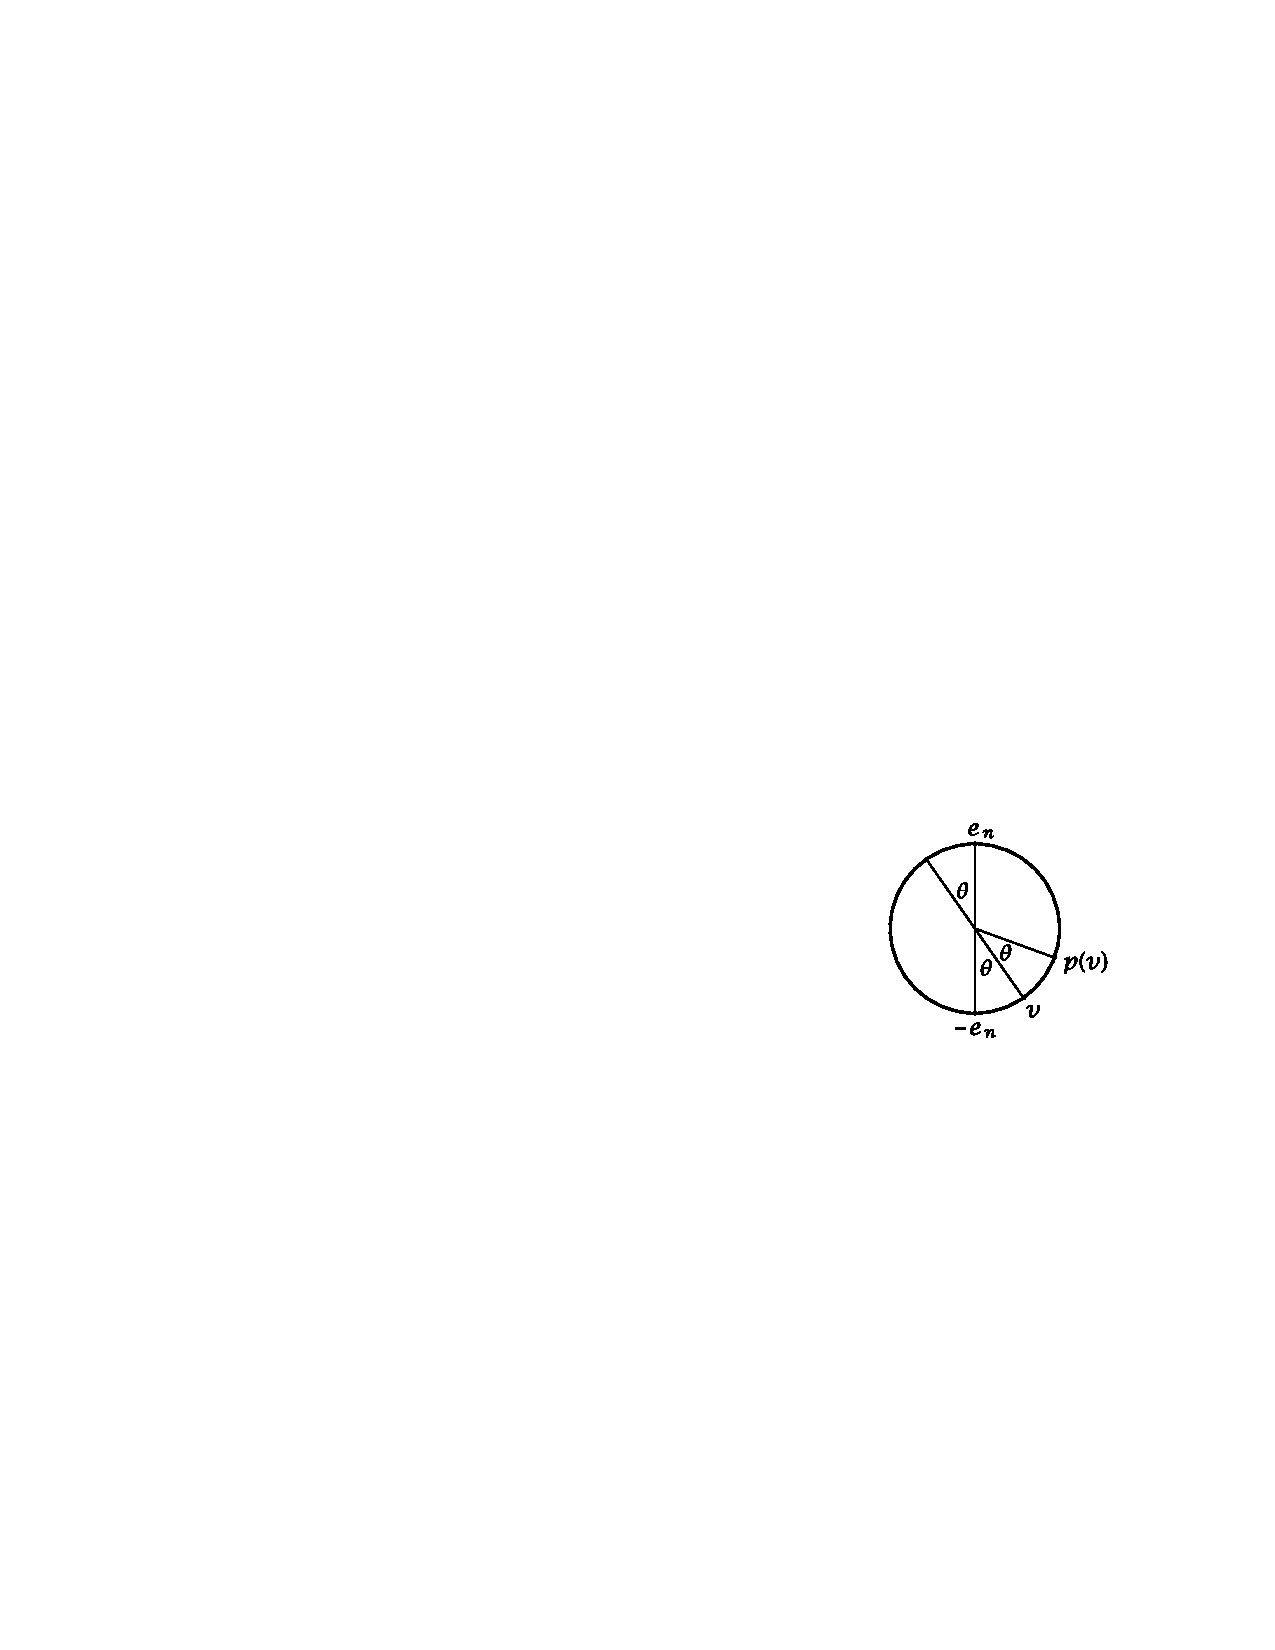
\includegraphics[scale=0.7]{figures/CW_SOn.pdf}
        \caption{Reflections defined in the proof of Proposition~\ref{prop 3D.1 Hatcher}.}
        \label{fig:CW_SOn}
    \end{figure}
    
    Statements (1) and (2) can now be proven by induction on $n$. The map $\rho$ takes $P^{n-2}$ to $\SO_{n-1}$, so we may assume inductively that the maps $\rho\circ\varphi^I$ for $I$ ranging over admissible sequences with first term $i_1<n-1$ are the characteristic maps for a $CW$-structure on $\SO_{n-1}$, with cells the corresponding products $e^I$. The admissible sequences $I$ with $i_1=n-1$ then give disjoint cells $e^I$ covering $\SO_n\setminus\SO_{n-1}$ by what was shown in the previous paragraph. So (1) and (2) hold for $\SO_n$.

    To prove (3) it suffices to show that there is an inclusion $P^iP^i\subset P^iP^{i-1}$ in $\SO_n$ since for an admissible sequence $I$, the map $\rho:P^I\to\SO_n$ takes the boundary of the top-dimensional cell of $P^I$ to the image of products $P^J$ with $J$ obtained from $I$ by decreasing one term $i_j$ by $1$, yielding a sequence which is admissible except perhaps for having two successive terms equal. As a preliminary to showing that $P^iP^i\subset P^iP^{i-1}$, observe that for $g\in \Or_n$ we have $r(g\cdot v)=gr(v)g^{-1}$. Hence $\rho(v)\rho(w)=r(v)r(\bf{e}_1)r(w)r(\bf{e}_1)=r(v)r(w')$ where $w'=r(\bf{e}_1)\cdot w$. Thus to show $P^iP^i\subset P^iP^{i-1}$ it suffices to find for each pair $v,w\in\bbR^{i+1}$ a pair $x\in\bbR^{i+1}$, $y\in\bbR^i$ with $r(v)r(w)=r(x)r(y)$.

    Let $V\subset \bbR^{i+1}$ be a 2-dimensional subspace containing $v$ and $w$. Since $V\cap \bbR^i$ is at least 1-dimensional, we can choose a unit vector $y\in V\cap \bbR^i$. Let $g\in\Or_{i+1}$ take $V$ to $\bbR^2$ and $y$ to $\bf{e}_1$. Then the conjugate $gr(v)r(w)g^{-1}=r(g\cdot v)r(g\cdot w)$ lies in $\SO_2$, hence has the form $\rho(z)=r(z)r(\bf{e}_1)$ for some $z\in\bbR^2$ by statement (2) for $n=2$. Therefore
    \[r(v)r(w)=g^{-1}r(z)r(\bf{e}_1)g=r(g^{-1}\cdot z)r(g^{-1}\cdot \bf{e}_1)=r(x)r(y)\]
    for $x=g^{-1}\cdot z\in\bbR^{i+1}$ and $y\in\bbR^i$.

    It remains to show that the map $\rho:P^{n-1}\times P^{n-2}\times\cdots\times P^1\to \SO_n$ is cellular. This follows from the inclusions $P^iP^i\subset P^iP^{i-1}$ derived above, together with another family of inclusions $P^iP^j\subset P^j P^i$ for $i<j$. To prove the latter we have the formulas
    \begin{align}
        \rho(v)\rho(w)&=r(v)r(w')\text{ where }w'=r(\bf{e}_1)\cdot w \notag\\
        &=r(v)r(w')r(v)r(v)\notag\\
        &=r(r(v)\cdot w')r(v)\text{ from }r(g\cdot v)=gr(v)g^{-1}\notag\\
        &=r(r(v)r(\bf{e}_1)\cdot w)r(v)=r(\rho(v)\cdot w)r(v)\notag\\
        &=\rho(\rho(v)\cdot w)\rho(v')\text{ where }v'=r(\bf{e}_1)\cdot v,\text{ hence }v=r(\bf{e}_1)\cdot v'.
    \end{align}
    In particular, taking $v\in\bbR^{i+1}$ and $w\in\bbR^{j+1}$ with $i<j$, we have $\rho(v)\cdot w\in\bbR^{j+1}$, and the product $\rho(v)\rho(w)\in P^iP^j$ equals the product $\rho(\rho(v)\cdot w)\rho(v')\in P^jP^i$.
\end{proof}


This result can be used to easily compute the homology groups of $\SO_n$, as is done in \cite{Hatcher}. $CW$-structures also exist on $\SU_n$ and $\Sp_n$. We don't describe them since for us it will only be important to know that they exist. Instead of using these $CW$-structures directly, we will use exact sequences of homotopy groups to compute \emph{some} homotopy groups of the classical groups.





\subsection{Lie group actions I} \label{sec: Lie group actions}

\begin{defn}[Lie group action]\index{Lie group action}
    Given a Lie group $G$ and a smooth manifold $M$, a Lie group action of $G$ on $M$ is a smooth map $\Phi:G\times M\to M$ such that, denoting $\Phi_g=\Phi(g,\_):M\to M$, it holds that \[\Phi_e=\id_M,\] and either
    \[\Phi_{gh}=\Phi_g\circ \Phi_h\quad  \text{    (left action)}\]
    or
    \[\Phi_{gh}=\Phi_h\circ \Phi_g\quad  \text{(right action)}.\]

    In particular, each $\Phi_g$ is a diffeomorphism on $M$. As before, we will sometimes simply write $g\cdot x=\Phi(g,x)$ for left actions and $x\cdot g=\Phi(g,x)$ for right actions. The triple $(M,G,\Phi)$ is referred to as a Lie group action and the pair $(M,\Phi)$ as a $G$-manifold. When the name of the action is not needed, we will simply write $G\acts M$ for a left action and $M\lacts G$ for a right one.
\end{defn}

The notions of orbits, stabilizers, transitive actions and free actions transfer with no changes to the context of Lie groups.

\begin{example}[Actions of $G$ on itself]
    The left and right translation operators $L_g,R_g$ on a Lie group $G$ are smooth diffeomorphisms since $(L_g)^{-1}=L_{g^{-1}}$ is a smooth inverse. In addition,
    \[L_{gh}=L_g\circ L_h,\quad R_{gh}=R_h\circ R_g.\]
    Therefore $L_g$ defines a left action of $G$ on itself, and $R_g$ defines a right action. Note that these two actions commute: 
    \[L_g\circ R_h=R_h\circ L_g.\]
    
    In addition, the adjoint operator $\Adg_g$ defines the \emph{adjoint action} of $G$ on itself since 
    \[\Adg_{gh}=\Adg_g\circ \Adg_h,\]
    which makes it a left action. Similarly, $\Adg_{g^{-1}}$ is a right action.
\end{example}

\begin{example}[Lie group actions]
    \begin{enumerate}[label=(\alph*)]
        \item The natural action of $\GL_n(V)$ on $V$ via $(A,x)\mapsto Ax$ is a smooth left action.
        \item An action of a discrete group $\Gamma$ on a manifold is smooth iff every $\Phi_g$ is smooth. E.g.~$\bbZ^n$ acts smoothly and freely on $\bbR^n$ by translations $(n,x)\mapsto x+n$.
        \item The automorphism group $\Aut(\pi)$ of a smooth covering map $\pi:E\to M$ is a zero-dimensional Lie group acting smoothly and freely on $E$.
    \end{enumerate}
\end{example}

\begin{defn}[Equivariant maps]\index{Equivariant maps}
    Let $G$ be a Lie group, and let $(M,\Phi)$ and $(M',\Phi')$ be smooth manifolds endowed with smooth left or right $G$-actions $\Phi$ and $\Phi'$. A map $F:M\to M'$ is called $G$-equivariant with respect to the given $G$-actions if
    \[F\circ \Phi_g=\Phi_g' \circ F\]
    for all $g\in G$.
    In other words, the following diagram must commute:
    \[
    \begin{tikzcd}[every matrix/.append style={name=m}]
       M \arrow[r,"F"]\arrow[d,"\Phi_g",swap] & M'\arrow[d,"\Phi_g'"]\\
       M \arrow[r,"F", swap] & M'.
    \end{tikzcd}
    \]
    This condition is also often expressed by saying \emph{$F$ intertwines $\Phi$ and $\Phi'$}. Equivariant maps comprise the morphisms of the category $G\mathsf{-Man}^\infty$ of smooth manifolds with a $G$-action.

    Furthermore, for two Lie group actions $(M_i,G_i,\Phi^i)$, $i=1,2$, a morphism between them is a pair $(\varphi,\rho)$ consisting of a smooth map $F:M_1\to M_2$ and a Lie group homomorphism $\rho:G_1\to G_2$ such that the corresponding square commutes:
    \[F\circ \Phi^1=\Phi^2\circ \left(\rho\times F \right).\]
    In this case we say that $F$ intertwines the actions $\Phi^i,i=1,2$.
\end{defn}

\begin{example}
    The map $\exp:\bbR^n\to \bbT^n$ given by $\exp(x^1,\ldots,x^n)=(\rme^{2\pi\rmi x^1},\ldots,\rme^{2\pi\rmi x^n})$ is a smooth map that intertwines the actions of $\bbR$ on $\bbR^n$ and $\bbT^n$ by
    \begin{align}
        t\in\bbR\text{ acting on }\bbR^n:\;\quad t\cdot x&=x+tv,\\
        t\in\bbR\text{ acting on }\bbT^n:\; (t\cdot z)^k&=\rme^{2\pi\rmi tv^k}z^k,
    \end{align}
    where $v\in\bbR^n$ is a fixed vector.
\end{example}

\begin{thm}[Equivariant rank theorem {{\cite[Thm.~7.25]{Lee}}}]\label{thm equivariant rank}\index{Theorem!Equivariant rank}
    Let $F:(M,\Phi)\to F(M',\Phi')$ be a smooth $G$-equivariant map and let the action $\Phi$ be transitive. Then $F$ has constant rank.
\end{thm}
\begin{proof}
    Let $p,q\in M$, and let $g\in G$ be such that $\Phi_g(p)=q$ (it exists by transitivity). By computing the differential of the equivariance condition, we get
    \[T_qF\circ T_p\Phi_g=T_{F(p)}\Phi_g'\circ T_pF.\]
    Since the differentials of group actions are isomorphisms of vector spaces, the other two maps have the same rank. This means that $F$ has the same rank at any two points.
\end{proof}


\begin{defn}[Orbit map]\index{Orbit map}
    Given a Lie group action $\Phi:G\times M\to M$, for each $p\in M$ we define the smooth orbit map 
    \[\Phi^p:G\to M,\quad g\mapsto \Phi(g,p).\]
\end{defn}

\begin{prop}[{{\cite[Prop.~7.26]{Lee}}}]
    The orbit map $\Phi^p:G\to M$ defined above has constant rank, so the stabilizer $G_p=(\Phi^p)^{-1}(p)$ is a properly embedded Lie subgroup of $G$. If $G_p=\{e\}$, then $\Phi^p$ is an injective smooth immersion, so the orbit $\Phi(G,p)$ is an immersed submanifold of $M$.
\end{prop}
\begin{proof}
    First we note that $\Phi^p$ intertwines the left action of $L_g$ on $G$ and $\Phi$ on $M$. Since $G$ acts transitively on itself, $\Phi^p$ has constant rank by Theorem~\ref{thm equivariant rank}. Thus $G_p$ is properly embedded by Theorem~\ref{thm level set submanifold} and a Lie subgroup by Proposition~\ref{prop 7.11 Lee}.

    If $G_p=\{e\}$, then $\Phi^p$ is injective, and therefore by the Equivariant Rank Theorem~\ref{thm equivariant rank} it is a smooth immersion (recall that an injective map of constant rank is an immersion by the Global Rank Theorem~\ref{Global rank}). This makes the orbit an immersed submanifold by Proposition~\ref{prop 5.18 Lee}.
\end{proof}
\begin{rem}
    We will later prove that the condition on the stabilizer subgroup can be dropped.
\end{rem}

% \begin{example}[Classical groups]\index{Group!classical}
%     \begin{enumerate}[label=(\alph*)]
%         \item $\Or_n(\bbR)$ is the level set $F^{-1}(\rmI_n)$ of the map $F:\GL_n(\bbR)\to \Mat_n(\bbR)$, $A\mapsto A^TA$. $F$ intertwines the right action of $\GL_n(\bbR)$ on itself with its right action $B\mapsto B^TAB$ on $\Mat_n(\bbR)$ (both actions are clearly smooth). Thus $\Or_n(\bbR)$ is a properly embedded Lie subgroup of $\GL_n(\bbR)$. It is compact because it is closed and bounded in $\Mat_n(\bbR)$: closed because it is a level set of $F$, and bounded because the matix norm of each orthogonal matrix is $\sqrt{n}$.
%         \item $\SO_n(\bbR)$ is the identity component of $\Or_n(\bbR)$, which is also the set of orthogonal determinant that have determinant $+1$ and thus preserve spatial orientations. Therefore it is an open Lie subgroup of $\Or_n(\bbR)$.
%         \item $U_n\subset \GL_n(\bbC)$ is defined similarly as the level set of $A\mapsto A^\ast A$ and is therefore a properly embedded Lie subgroup of $\GL_n(\bbC)$ of real dimension $n^2$. $\SU_n=\U_n\cap \SL_n(\bbC)$ and it is easy to check that $\SU_n$ is a properly embedded Lie subgroup of $U_n$ of real dimension $n^2-1$.
%     \end{enumerate}
% \end{example}







\subsection{Semidirect products}

\begin{defn}[Semidirect product]\index{Semidirect product}
    A smooth left action $\Phi:H\times N\to N$ of a Lie group $H$ on another Lie group $N$ is called an action by automorphisms if the maps $\Phi_h:N\to N$ are group automorphisms for all $h\in H$. 

    Given such an action, the semidirect product of $H$ and $N$ is, denoted $N\rtimes_\Phi H$ as a manifold, the Cartesian product $N\times H$, endowed with the multiplication
    \[(n,h)(n',h')=(n\Phi_h(n'),hh').\]
\end{defn}
It is easy to check that the product defined above is a valid group product, and it's clearly smooth along with its inverse $(n,h)^{-1}=(\Phi_h^{-1}(n^{-1}),h^{-1})$.

\begin{example}[The Euclidean group]\index{Group!Euclidean}
    $\Or_n(\bbR)$ acts by automorphisms on the translation group $\bbR^n$. Their semidirect product is the Euclidean group $\rmE_n=\bbR^n\rtimes \Or_n(\bbR)$:
    \[(b,A)(b',A')=(n+An',AA').\]
    It also acts on $\bbR^n$ via 
    \[(b,A)\cdot x=b+Ax.\]
\end{example}


The following two theorems are a simple exercise.
\begin{prop}[Properties of semidirect products]
    Let $G=H\ltimes_\Phi N=N\rtimes_\Phi H$ as above.
    \begin{enumerate}[label=(\alph*)]
        \item The subsets $\wt{N}=N\times\{e\}$ and $\wt{H}=\{e\}\times H$ are closed Lie subgroups of $G$ isomorphic to $N$ and $H$, respectively.
        \item $\wt N$ is a normal subgroup of $G$.
        \item $\wt N\cap \wt H=\{(e,e)\}$ and $\wt{N}\wt{H}=G$.
    \end{enumerate}
\end{prop}

\begin{thm}[Characterization of semidirect products]
    Let $N,H\subset G$ be closed Lie subgroups of a Lie group $G$ such that $N$ is normal, $N\cap H=\{e\}$, and $NH=G$. Then the map $(n,h)\mapsto nh$ is a Lie group isomorphism between $H\ltimes_{\Ad} N$ and $G$, where $\Ad:H\times N\to N$ is the adjoint action $\Ad_h(n)=hnh^{-1}$.
\end{thm}
This kind of a semiproduct is called \emph{internal}, but this theorem essentially shows that every semidirect product is internal with respect to the resulting group.

\begin{xca}
    Show the following isomorphisms (recall that in a semidirect product $N\rtimes H$, $N$ is a normal subgroup):
    \begin{enumerate}[label=(\alph*)]
        \item $\Or_n(\bbR)\cong \SO_n(\bbR)\rtimes \Or_1$.
        \item $\U_n(\bbR)\cong \SU_n(\bbR)\rtimes \U_1$.
        \item $\GL_n(\bbR)\cong \SL_n(\bbR)\rtimes \bbR^\times$.
        \item $\GL_n(\bbC)\cong \SL_n(\bbC)\rtimes \bbC^\ast$.
    \end{enumerate}
    Prove that none of these groups are isomorphic to the analogous direct product groups by comparing the centers (the center is the set of all elements that commute with all of $G$).
\end{xca}



An important class of matrix Lie groups closely related to classical groups are affine groups, extending the definition of the Euclidean group above.

\begin{defn}[Affine extension]\index{Affine extension}
    Let $G\sub \GL_n(\bbK)$, where $\bbK=\bbR$ or $\bbC$, be a matrix Lie group. The \emph{affine extension} of $G$ is the semidirect product 
    \[\rmA G\coloneqq G\ltimes \bbK^n,\]
    where the canonical action of $G$ on $\bbK^n$ is implied. The resulting normal subgroup $\bbK^n$ is called the \emph{group of translations}. $\rmA G$ is isomorphic to the subgroup of $\GL_{n+1}(\bbK)$ consisting of matrices of the block form
    \[\begin{bmatrix}
        g & \bf{x}\\
        \bf{0}_n^T & 1
    \end{bmatrix},\quad g\in G,\; \bf{x}\in\bbK^n,\]
    where $\bf{0}_n^T$ is a row of $n$ zeros. From here, it is easy to see that the correspondence $G\mapsto \rmA G$ is a functor.
\end{defn}

\begin{example}
    \begin{enumerate}
        \item $\Aff_n(\bbK)\coloneqq \rmA \GL_n(\bbK)=\GL_n(\bbK)\ltimes\bbK^n$ is the \emph{affine group}.\index{Group!Affine}
        \item $\rmA \SL_n(\bbR)=\SL_n(\bbR)\ltimes \bbR^n$ is the \emph{equi-affine group}.\index{Group!Equi-affine}
        \item $\SE_n\coloneqq \rmA \SO_n{}= \SO_n\ltimes\bbR^n$ is the \emph{special Euclidean group}.\index{Group!Special Euclidean}
    \end{enumerate}
\end{example}










\subsection{Representations}

\begin{defn}[Linear representation]\index{Lie group!representation}
    Let $\bbK$ be either $\bbR$ or $\bbC$. A $\bbK$-linear representation of a Lie group $G$ is a $\bbK$-vector space $V$ with a smooth left $G$-action $\Phi$ such that each map $\Phi_g:V\to V$ is a $\bbK$-linear automorphism. Equivalently, a representation is a smooth homomorphism $\rho=\Phi_\bullet:G\to \GL_{\bbK}(V)$. 

    A representation $\rho :G\to \GL(V)$ is called \emph{faithful} if it is injective.
\end{defn}
Note that in principle it is possible do define infinite-dimensional representations even of finite-dimensional groups, but it will take some extra work to introduce the proper topology and smooth structure in that case.

\begin{example}[Lie group representations]\label{ex Lie group representations}
    \begin{enumerate}[label=(\alph*)]
        \item If $G$ is any Lie subgroup of $\GL_n(\bbR)$ (such groups are called \emph{matrix groups}), the inclusion map $G\hookrightarrow \GL_n(\bbR)$ is a faithful representation, called the \emph{defining representation of $G$}.
        \item The inclusion map $\bbS^1\hookrightarrow\bbC^\ast=\GL_1(\bbC)$ is a faithful representation of the circle group.
        \item Let $\sigma:\bbR^n\to \GL_{n+1}(\bbR)$ be the map that sends $x\in\bbR^n$ to the matrix $\sigma(x)$ defined in block form by 
        \[\sigma(x)=\begin{pmatrix}
            \rmI_n & x\\
            0 & 1
        \end{pmatrix},\]
        where $\rmI_n$ is the $n\times n$ identity matrix and $x$ is regarded as an $n\times 1$  column matrix. Then $\sigma$ is a faithful representation of the additive group $\bbR^n$.
        \item A faithful representation of the Euclidean group $\SE_n$ is given by $\rho:\SE_n\to \GL_{n+1}(\bbR)$ defined in block form by
        \[\rho(b,A)=\begin{pmatrix}
            A & b\\
            0 & 1
        \end{pmatrix},
        \]
        where $b$ is considered as a column.
        \item For positive integers $n$ and $d$, let $P^n_d$ denote the vector space of real polynomials $p:\bbR^n\to \bbR$ of degree at most $d$. For a matrix $A\in\GL_n(\bbR)$ define the linear map $\tau(A):P^n_d\to P^n_d$ by
        \[\tau(A)p=p\circ A^{-1}.\]
        This is a faithful representation of $\GL_n(\bbR)$.

        \item Another very important type of representation that is not linear is a projective representation, which is a homomorphism into the group $\PGL(V)=\GL(V)\slash (\bbK I)$ (where $\bbK I$ is the subgroup of multiplications by a scalar, which is also the center of $\GL(V)$) of projective linear transformations of a vector space. The projective special linear group $\PSL_2(\bbC)=\SL_2(\bbC)\slash\{I,-I\}$, also isomorphic to the proper orthochronous Lorentz group $\SO^+(1,3)$, acts on the projective complex line $\CP^1\cong \bbC\cup\{\infty\}$ via M\"obius transformations
        \[\begin{pmatrix}
            a & b\\
            c& d
        \end{pmatrix} \cdot z=\frac{az+b}{cz+d}.\]
        It is easy to check that this is a left action. It is \emph{sharply 3-transitive}, meaning that for any triple of points $(z,w,x)$ there exists a unique matrix $g\in \PSL_2(\bbC)$ that maps them to $(0,1,\infty)$.
    \end{enumerate}
\end{example}

\begin{xca}\label{xca psl=pgl}
    Show that $\PSL_n(\bbK)\cong \PGL_n(\bbK)$ iff every element of $\bbK$ has an $n$-th root.
\end{xca}

\begin{rem}
    Classical Lie groups are defined as groups of invertible matrices, and those matrices comprise the so called \emph{defining representations} of those groups. Moreover, very often in introductory courses on Lie groups it is assumed that all groups under consideration are matrix groups. It is therefore natural to ask whether every Lie group is isomorphic to some matrix group (such groups are also called \emph{linear}).\index{Linear group} The answer is no: not every finite-dimensional Lie group has a finite-dimensional faithful representation. The simplest example of a \emph{nonlinear} group is $\widetilde{\SL_2}(\bbR)$, the universal covering group of $\SL_2(\bbR)$. \index{Nonlinear group} We will be able to show that it can't have a faithful representation later (see Example~\ref{ex SL2R nonlinear}). Spin groups in even dimensions are also nonlinear. The fact of existence of such Lie groups is the ultimate justification for using general differential geometry to study them.
\end{rem}

Every Lie group has a canonical representation on its own tangent space at the identity.

\begin{defn}[Adjoint representation]\index{Adjoint representation}
    The derivative of the adjoint action at the identity, $T_e\Adg_g:T_e G\to T_e G$, is a linear representation of $G$. We use the same symbol without boldface to denote it:
    \[\Ad_g X=(\Adg_g)_{\ast e}(X).\]
    To further differentiate them, we will omit parentheses when writing the linear map $\Ad_g X$ but keep them when writing $\Adg_g(h)$.
\end{defn}

    Note that any abelian Lie group has a trivial adjoint representation ($\Ad_g=0$ for all $g\in G$).

\begin{example}[Adjoint representation of matrix groups]
    Let $G\subset \GL(V)$ be a matrix group. Then $T_e G\cong \Mat(V)$ and we can explicitly compute the adjoint representation. Since $\GL(V)$ is open in $\Mat(V)$, we can define a straight path $\gamma(t)=A+tX$ for any $A\in \GL(V)$ and $X\in \Mat(V)$. In particular, let $h(t)=I+tX$. Then for any $A\in \GL(V)$, using formula (\ref{eq differential in local coordinates}) for the action of a differential of a smooth map,
    \[\Ad_A X=\restr{\frac{\dd}{\dd t}}{t=0}A(I+tX)A^{-1}=AXA^{-1}.\]
    In other words, on matrix groups the Lie algebraic version of the adjoint map is still just matrix conjugation.
\end{example}






\subsection{Lie algebras: Construction I}

Since Lie groups are manifolds, the next most natural thing to do is to study its tangent spaces and to see what kind of structure on them is induced by the group structure. 
First we note that since $L_g:G\to G$ is a diffeomorphism for every $g\in G$, it induces the isomorphisms
\[(L_g)_{\ast e}: T_e G\to T_g G\]
between the tangent spaces at the identity and any other point. Moreover, since $L_{gh}=L_g\circ L_h$, the chain rule for derivatives implies that $(L_g)_\ast$ is natural in the sense that it truly depends only on $g$ itself and not how it might be decomposed into a product of other group elements.

Since Lie group homomorphisms preserve the identity, their derivatives map $T_e G$ to $T_eH$. Therefore it will completely suffice to study the properties of the tangent space at the identity.


First let us try to gain some intuition for how the group structure of $G$ might be ``encoded'' in $T_e G$ by working in local coordinates. Suppose $(U,\varphi)$ is a symmetric (i.e.~$U^{-1}=U$) open neighborhood of $e\in G$ and $\varphi:U\to \bbR^n$ a chart map on it such that $\varphi(e)=0$. We can find a smaller open neighborhood $U_0\subset U$ such that the the multiplication map $m:G\to G\to G$ restricts to $m:U_0\times U_0\to U$. The inversion map also restricts to $i:U\to U$. Then let $\mu:\varphi (U_0)^2\to \varphi(U)$ and $\iota:\varphi(U)\to \varphi(U)$ be their representatives in the local chart. Since these are now smooth maps on Euclidean spaces, we can study their Taylor series at the origin. Since $m(e,g)=m(g,e)=g$ for all $g$, we have
\[\mu(0,\bf{x})=\mu(\bf{x},0)=\bf{x}\]
for all $\bf{x}\in U_0$. This implies that both partial derivatives of $\mu$ computed at $(0,0)$ are the identity. Therefore the Taylor series of $\mu$ around the origin has the form
\[\mu(\bf{x},\bf{y})=\bf{x}+\bf{y}+\beta(\bf{x},\bf{y})+\gamma(\bf{x},\bf{y})+\calO(4),\]
where $\beta(\bf{x},\bf{y}):\varphi(U_0)^2\to \bbR^n$ is some vector-valued bilinear form of $\bf{x},\bf{y}\in\bbR^n$, $\gamma(\bf{x},\bf{y})$ is a similar cubic term, and $\calO(4)$ stands for terms that are quartic in $\bf{x}$ and $\bf{y}$ together ($\bf{x}^4, \bf{x}^3 \bf{y},$ etc.). In addition, since $m(g,i(g))=e$, we also have
\[\mu(\bf{x},\iota(\bf{x}))=\mu(\iota(\bf{x}),\bf{x})=0,\]
which implies that the Taylor series of the inversion map has the form
\[\iota(\bf{x})=-\bf{x}+\beta(\bf{x},\bf{x})+\calO(\bf{x}^3).\]

The extra constraints on the forms $\beta$ and $\gamma$ will come from the fact that they're not just some vector-valued forms, but that due to the group structure $m:G\times G\to G$ the domain and codomain of these forms are closely connected to each other. 



\begin{lem}
    The antisymmetric quadratic form
    \[b:\bbR^n\times\bbR^n\to \bbR^n,\quad b(\bf{x},\bf{y})=\beta(\bf{x},\bf{y})-\beta(\bf{y},\bf{x}),\]
    is natural with respect to local coordinate transformations on $G$. That is, for any matrix $A\in\GL_n(\bbR)$,
    \[A b(\bf{x},\bf{y})=b(A\bf{x},A\bf{y}).\]
\end{lem}
\begin{proof}
    Any local coordinate transformation on $U_0$, represented by a transition diffeomorphism $f$ with $f(0)=0$, will transform the local multiplication map $\mu$ into $\wt{\mu}$ with
    \[f(\wt\mu(\bf{x},\bf{y}))=\mu(f(\bf{x}),f(\bf{y})).\]
    Writing the Taylor series of $f$ as
    \[f(\bf{x})=A\bf{x}+f_2(\bf{x})+\calO(3),\]
    where $A$ is the Jacobi matrix of $f$ at the origin and $f_2(\bf{x})$ is the quadratic term, we have
    \[\mu(f(\bf{x}),f(\bf{y}))=A\bf{x}+A\bf{y}+f_2(\bf{x})+f_2(\bf{y})+\beta(A\bf{x},A\bf{y})+\calO(3)\]
    and
    \[f(\wt\mu(\bf{x},\bf{y}))=A\bf{x}+A\bf{y}+A\wt\beta(\bf{x},\bf{y})+f_2(\bf{x}+\bf{y})+\calO(3).\]
    By comparing these two expressions we conclude that
    \[f_2(\bf{x})+f_2(\bf{y})+\beta(A\bf{x},A\bf{y})=A\wt\beta(\bf{x},\bf{y})+f_2(\bf{x}+\bf{y}).\]
    In other words, the quadratic part of the multiplication map also depends on the quadratic part of the coordinate map itself. However, by noticing that the terms depending on $f_2$ are symmetric in $\bf{x}$ and $\bf{y}$, we get the statement of the theorem.
\end{proof}

This indicates the existence of a natural antisymmetric bilinear form $T_e G\times T_eG\to T_e G$. So far we have only used the property of the identity $eg=ge=g$. Aside from this, group multiplication also satisfies associativity.

\begin{lem}\label{3975}
    The associativity of group multiplication implies that
    \[
        \beta(\beta(\bf{x},\bf{y}),\bf{z})+\gamma(\bf{x},\bf{y})+\gamma(\bf{x}+\bf{y},\bf{z})
        =\beta(\bf{x},\beta(\bf{y},\bf{z}))+\gamma(\bf{y},\bf{z})+\gamma(\bf{x},\bf{y}+\bf{z}).
    \]
\end{lem}
\begin{proof}
    We have 
    \begin{multline}
        \mu(\mu(\bf{x},\bf{y}),\bf{z})=\bf{x}+\bf{y}+\beta(\bf{x},\bf{y})+\gamma(\bf{x},\bf{y})
        +\bf{z}+\beta(\bf{x}+\bf{y},\bf{z})+\beta(\beta(\bf{x},\bf{y}),\bf{z})+\\+\gamma(\bf{x}+\bf{y},\bf{z})+\calO(4)
    \end{multline}
    and 
    \begin{multline}
        \mu(\bf{x},\mu(\bf{y},\bf{z}))=\bf{x}+\bf{y}+\bf{z}+\beta(\bf{x},\bf{y}+\bf{z})+\beta(\bf{y},\bf{z})
        +\gamma(\bf{y},\bf{z})+\beta(\bf{x},\beta(\bf{y},\bf{z}))+\\+\gamma(\bf{x},\bf{y}+\bf{z})+\calO(4).
    \end{multline}
    These two expressions must be equal by associativity. All terms of degree less than 3 cancel out because $\beta$ is bilinear, and we get the claimed formula.
\end{proof}

\begin{lem}
    The antisymmetric form $b(\bf{x},\bf{y})$ satisfies the Jacobi identity
    \[b(\bf{x},b(\bf{y},\bf{z}))+b(\bf{y},b(\bf{z},\bf{x}))+b(\bf{z},b(\bf{x},\bf{y}))=0.\]
\end{lem}
\begin{proof}
    We antisymmetrize the equation from Lemma~\ref{3975} with respect to permutations of all three arguments. First we notice that the antisymmetrization of $\gamma(\bf{x},\bf{y})$ will be the same as that of $\gamma(\bf{y},\bf{z})$ since they are related to each other by a cyclic (and thus even) permutation. Moreover, the antisymmetizations of both $\gamma(\bf{x}+\bf{y},\bf{z})$ and $\gamma(\bf{x},\bf{y}+\bf{z})$ vanish since both of these are symmetric under a transposition of two of the arguments, and the only function that is both symmetric and antisymmetric is zero.

    What remains is 
    \[\Alt \beta(\beta(\bf{x},\bf{y}),\bf{z})=\Alt \beta(\bf{x},\beta(\bf{y},\bf{z})),\]
    where $\Alt$ is the antisymmetrization operator 
    \[\Alt f(\bf{x}_1,\bf{x}_2,\bf{x}_3)=\sum_{\sigma\in S_3}\sign(\sigma)f(\bf{x}_{\sigma(1)},\bf{x}_{\sigma(2)},\bf{x}_{\sigma(3)}).\]

    This equation has six terms on each side, and we are going to group them into three groups of four by gathering terms that have the same variable standing alone. We start with those having $\bf{z}$ as a lone variable. On the left hand side we combine two terms coming from the transposition $(1\Leftrightarrow2)$
    \[\beta(\beta(\bf{x},\bf{y}),\bf{z})-\beta(\beta(\bf{y},\bf{x}),\bf{z})=\beta(b(\bf{x},\bf{y}),\bf{z}),\]
    whereas on the right hand side we find
    \[\beta(\bf{z},\beta(\bf{x},\bf{y}))-\beta(\bf{z},\beta(\bf{y},\bf{x}))=\beta(\bf{z},b(\bf{x},\bf{y})).\]
    Finally, bringing these two expressions to the same side we find
    \[\beta(b(\bf{x},\bf{y}),\bf{z})-\beta(\bf{z},b(\bf{x},\bf{y}))=b(b(\bf{x},\bf{y}),\bf{z}).\]
    The full antisymmetrization is just a sum of cyclic permutations of this one, which gives us the Jacobi identity.
\end{proof}

\begin{rem}
    It's always possible to find some local coordinates in which $\beta(\bf{x},\bf{y})=\frac12 b(\bf{x},\bf{y})$ is antisymmetric right away (namely the coordinates in which $\iota(\bf{x})=-\bf{x}+\calO(\bf{x}^3)$). Later we will prove the miraculous result that there is a special coordinate system in which $\iota(\bf{x})\equiv-\bf{x}$ and not only the quadratic term, but \emph{all} higher terms in the Taylor series of $\mu(\bf{x},\bf{y})$ can be written in terms of \emph{only} $b(\bf{x},\bf{y})$, and there is a \emph{universal} formula giving this dependence (the Baker-Campbell-Hausdorff formula). In other words, the entire local structure of the Lie group is encoded in the bilinear form $b$.
\end{rem}



\subsection{Lie algebras: Construction II}

The above calculations can be circumvented if we display a manifestly functorial object that gives an antisymmetric bilinear form on $T_eG$. To this end, let us take a look at the local representation of the conjugation map $\Ad_g h=ghg^{-1}$:
\[c(\bf{x},\bf{y})=\mu(\mu(\bf{x},\bf{y}),\iota(\bf{x})).\]

\begin{lem}
    The Taylor series of the local conjugation map reads
    \[c(\bf{x},\bf{y})=\bf{y}+b(\bf{x},\bf{y})+\calO(3).\]
\end{lem}
\begin{proof}
Combining the Taylor series of $\mu$ and $\iota$, we have
    \begin{multline}
        \mu(\mu(\bf{x},\bf{y}),\iota(\bf{x}))= \bf{x}+\bf{y}+\iota(\bf{x})+\beta(\bf{x}+\bf{y},\iota(\bf{x})) +\beta(\bf{x},\bf{y})+\calO(3)=\\
        =\bf{x}+\bf{y}-\bf{x}+\beta(\bf{x},\bf{x})+\beta(\bf{x},-\bf{x})+ \beta(\bf{y},-\bf{x})+ \beta(\bf{x},\bf{y})+\calO(3)=\\
        =\bf{y}+\beta(\bf{x},\bf{y})-\beta(\bf{y},\bf{x}) +\calO(3)=\bf{y}+b(\bf{x},\bf{y})+\calO(3).
    \end{multline}
\end{proof}

Moreover, since $c(\bf{x},0)=0$ for all $\bf{x}$ in some neighborhood of the origin, we know that the error term $\calO(3)$ vanishes when $\bf{y}=0$ and therefore is $\calO(3)=\bf{y}\calO(\bf{x}^2,\bf{x}\bf{y},\bf{y}^2)$. This means that the double derivative with respect to $\bf{x}$ and $\bf{y}$, which naturally acts on two vectors $\bf{X},\bf{Y}\in\bbR^n$ reads
\[\left(\frac{\partial^2}{\partial \bf{x}\partial \bf{y}}c(\bf{x},\bf{y})\right)(\bf{X},\bf{Y})=b(\bf{X},\bf{Y})+\calO(\bf{x},\bf{y})(\bf{X},\bf{Y}).\]
At $\bf{x}=\bf{y}=0$ the error term vanishes and we get
\[\left(\restr{\frac{\partial^2}{\partial \bf{x}\partial \bf{y}}}{\bf{x}=\bf{y}=0}c(\bf{x},\bf{y})\right)(\bf{X},\bf{Y})=b(\bf{X},\bf{Y}).\]

Obviously this double derivative is nothing but the local chart representation of the double derivative of $\Adg_g(h)= ghg^{-1}$ viewed as a map $G\times G\to G$ with respect to both variables. Recall that we call its derivative at the identity $(\Adg_g)_{\ast e}:T_eG\to T_e G$ by the symbol $\Ad_g$. We can now think of this as a map $\Ad_\bullet:G\to \GL(T_e G)$. With this, we have
\[T_{g=e}T_{h=e}(\Ad_g(h))=T_e \Ad_\bullet.\]
Note that the two derivatives commute because partial derivatives of smooth maps on $\bbR^n$ commute. This is a linear operator $T_e \Ad_\bullet:T_eG\to T_e\GL(T_e G)\cong \End(T_eG)$ from the tangent space $T_e G$ to the space of linear operators on it (this can also be thought of as a tensor on $T_e G$ of contravariant rank 1 and covariant rank 2). 

We will commonly denote elements of the Lie algebra by capital Latin letters to distinguish them from general tangent vectors and vector fields on Lie groups.

\begin{defn}[Adjoint operator, Lie bracket]
    The linear adjoint operator is
    \[\ad=T_e \Ad: \quad T_eG\to \End(T_eG).\]
    More explicitly, for every $A,B\in T_eG$, the action of $\ad_A:T_eG\to T_eG$ is defined by
    \[\ad_A B=(T_e(\Ad_\bullet B))(A).\]
\end{defn}

Equivalently, using the definition of tangent vectors as equivalence classes of curves, we have
\begin{multline}
    \ad_A B=\restr{\frac{\dd}{\dd t} \frac{\dd}{\dd s}}{t=s=0}g(t)h(s)g^{-1}(t)=\restr{\frac{\dd}{\dd t} \frac{\dd}{\dd s}}{t=s=0}g(t)h(s)g^{-1}(t)h^{-1}(s)=\\=\restr{\frac{\dd}{\dd t} \frac{\dd}{\dd s}}{t=s=0}{} [g(t),h(s)].\label{30071}
\end{multline}
for any two curves $g(t)$ and $h(s)$ such that $A=g'(0)$ and $B=h'(0)$. The fact that inserting the extra $h^{-1}(s)$ doesn't change the result is due to the fact that it can't contribute anything to the $\calO(ts)$ term in the Taylor series since the $\calO(t)$ term in $ghg^{-1}$ is already zero (to first order $ghg^{-1}$ in local coordinates reads $tA+sB-tA=sB$ as follows from our local functions $\mu$ and $\iota$). This identity can be treated as yet another construction of the Lie algebra, but we already know that it is equivalent to the others.

Note that in local coordinates the anti-symmetric form that we derived in the first construction is exactly the Lie bracket written in a local chart $(U,\varphi)$:
\[b(\varphi_{\ast e} A,\varphi_{\ast e} B)=\varphi_{\ast e}(\ad_A B).\]
The anti-symmetry and the Jacobi identity for $\ad_A B$ follow from those for $b(A,B)$.

\begin{defn}[Lie algebra]\index{Lie algebra}
    A Lie algebra is a pair $(\frakg,[\cdot,\cdot])$ where $\frakg$ is a finite-dimensional vector field over the field $\bbK$ and $[\cdot,\cdot]:\frakg\times\frakg\to\frakg$ is a map called a Lie bracket that satisfies the following properties for all $A,B,C\in \frakg$:
    \begin{enumerate}
        \item bilinearity: for all $a,b\in \bbK$,
        \[[aA+bB,C]=a[A,C]+b[B,C],\quad [A,aB+bC]=a[A,B]+b[A,C];\]
        \item alternating property:
        \[[A,A]=0;\]
        \item Jacobi identity:
        \[[[A,B],C]+[[B,C],A]+[[C,A],B]=0.\]
    \end{enumerate}
    Note that over fields of characteristic other than 2, like $\bbR$ or $\bbC$ the last two properties together imply skew-symmetry (anticommutativity) $[A,B]=-[B,A]$.

    A Lie subalgebra of $\frakg$ is a linear subspace $\frakh\subset\frakg$ such that $[\frakh,\frakh]\subset\frakh$, i.e.~the restriction of the Lie bracket to $\frakh$ produces a Lie bracket on $\frakh$ and the inclusion map is a homomorphism of Lie algebras. In this case we write $\frakh\leq \frakg$.
\end{defn}


\begin{example}
    Any associative algebra $(\calA,\cdot)$ (i.e.~a vector space with a binary associative multiplication operation) can be endowed with a structure of a Lie group by setting the Lie bracket as the commutator
    \[[A,B]=A\cdot B-A\cdot B.\]
    For example, the algebra $\Lin(V)=\End(V)$ of linear maps on a vector space $V$ admits this structure. In fact this is a forgetful functor $\mathsf{AssAlg}\to\mathsf{LieAlg}$.
\end{example}

Historically, most Lie algebras were ``discovered'' as not just the Lie algebras associated with associative rings (i.e.~commutator algebras), but as algebras of derivations on rings.

\begin{defn}[Derivation]\index{Derivation}
    Given a (not necessarily associative) ring $R$, a derivation on it is a map $D:R\to R$ that is additive ($D(x+y)=Dx+Dy$) and satisfies the Leibniz rule $D(xy)=Dx\cdot y+x\cdot Dy$.
\end{defn}

\begin{example}[Lie ring/algebra of derivations]
    Denote the set of all derivations on a ring $R$ by $\Der(R)$. Clearly the sum of two derivations is a derivation, however the composition is not always a derivation. However, it is easy to verify that the commutator $[D_1,D_2]=D_1D_2-D_2D_1$ of two derivations is a derivation. Thus $\Der(R)$ has a natural structure of a Lie ring. If $R=A$ is actually an algebra over some field, then $\Der(A)$ becomes a Lie algebra. As we will soon see, when $A$ is an algebra of smooth scalar functions, $\Der(A)$ consists of a certain type of differential operators.
\end{example}



\begin{defn}[Lie algebra homomorphism]
    Given two Lie algebras $\frakg,\frakg'$, a homomorphism $\phi:\frakg\to\frakg'$ is a linear map such that 
    \[\phi[A,B]_{\frakg}=[\phi A,\phi B]_{\frakg'}.\]
    These maps comprise the morphisms in the category $\mathsf{LieAlg}_{\bbK}$ of Lie algebras over the field $\bbK$.
\end{defn}


\begin{example}[Inner derivations on a Lie algebra]
    On any abstract Lie algebra $(\frakg,[\cdot,\cdot])$ one can define the linear adjoint operators $\ad_x:\frakg\to\frakg$ by $\ad_x(y)=[x,y]$. It is then easy to see that the Jacobi identity for $[\cdot,\cdot]$ is equivalent to the statement that $\ad_x$ is a derivation on $\frakg$:
    \[\ad_x([y,z])=[\ad_x y,z]+[y,\ad_x z].\]
    Moreover, since $\ad_x y=-\ad_y x$, this can also be written as
    \[\ad_{[x,y]}z=[\ad_x,\ad_y]z,\]
    which is equivalent to saying that $\ad:\frakg\to \mathfrak{gl}(\frakg)$ is a \emph{homomorphism} of Lie algebras. Therefore the set of all adjoint operators comprises a Lie subalgebra $\Inn(\frakg)\subset \mathfrak{gl}(\frakg)$, called the \emph{algebra of inner derivations} on $\frakg$.
\end{example}



Knowing from Construction I that $\ad_A B$ satisfies the properties of a Lie bracket, we can finally define the Lie algebra corresponding to a Lie group.

\begin{defn}[Lie algebra of a Lie group]
    Given a Lie group $G$, its Lie algebra is $\frakg=T_e  G$ with the Lie bracket $[A,B]=\ad_A B$. 
    
    The Jacobi identity can be alternatively written as
    \[\ad_A[B,C]=[\ad_A B,C]+[B,\ad_A C],\]
    which is equivalent to saying that the adjoint $\ad_A$ is a derivation with respect to the Lie bracket. 
\end{defn}

\begin{rem}[Gothic notation]
    It is conventional to use the gothic version of the symbol denoting the group for its Lie algebra, so $\GL_n\mapsto \frakgl_n$, $\SO_n\mapsto \frakso_n$, and so on. Sometimes we will use pairs of symbols $(G,\frakg)$, $(H,\frakh)$, etc., for Lie groups and their Lie algebras without explicitly stating that they correspond to each other. Moreover, since we will have several equivalent definitions of the Lie algebra $\frakg$ of a Lie group $G$, we will use $\frakg$ to refer to any of its isomorphic constructions depending on the situation.
\end{rem}

\begin{lem}\label{lem gl(V)}
    If $G=\GL(V)$ and $A,B\in T_e G\cong \End(V)$, then 
    \[\ad_A B=[A,B]=AB-BA.\]
\end{lem}
\begin{proof}
    As we've shown before, on matrix groups $\Ad_A B=ABA^{-1}$. Letting $a=\rmI+tA$ and noting that $a^{-1}=\rmI-tA+\calO(t^2)$, we find
    \[\Ad_{\rmI+tA} B=t(AB-BA)+\calO(t^2),\]
    which upon differentiation at $t=0$ implies the claimed formula.
\end{proof}


\begin{example}[$\mathfrak{gl}_n(R)$]
    The so called \emph{general linear Lie algebra} constructed in Lemma~\ref{lem gl(V)} is denoted $\mathfrak{gl}(V)=\End(V)^{(-)}$ (recall that $R\mapsto R^{(-)}$ is the forgetful functor that turns a ring into its associated Lie ring by defining the Lie bracket as the commutator). In fact it can be defined over all associative rings. Usually we use the standard basis consisting of the \emph{standard matrix units} $e_{ij},i\leq j$. Since $e_{jh}e_{ik}=\delta_{jh}e_{ik}$, the commutator reads
    \[[e_{ij},e_{hk}]=\delta_{jh}e_{ij}-\delta_{ki}e_{hj}.\]

    Later we will see that the Poincar\'e-Birkhoff-Witt Theorem implies that any Lie algebra $L$ is isomorphic to a subalgebra of some commutator Lie algebra $\calA^{(-)}$ of some associative algebra $\calA$. Moreover, the theorem of Ado and Iwasawa implies that for a finite-dimensional $L$ the algebra $\calA$ can be taken to be finite-dimensional.
\end{example}

\begin{example}[$\mathfrak{sl}_n(R)$]
    The commutator of any two traceless matrices is traceless, thus we have the Lie subalgebra of $\mathfrak{gl}_n(R)$ consisting of traceless matrices:
    \[\mathfrak{sl}_n(R)=\{x\in \mathfrak{gl}_n(R)\mid \tr x=0\},\]
    called the \emph{special linear Lie algebra}.
\end{example}

\begin{xca}
    Come up with a way to embed $\mathfrak{gl}_n(R)$ as a Lie subalgebra of $\mathfrak{sl}_{n+1}(R)$.
\end{xca}


Now it is instructive to repeat the derivation of the properties of this Lie bracket without reference to local coordinates. First, we prove its naturality.

\begin{prop}[{{\cite[Prop.~1.1.3]{DK}}}]\label{prop 1.1.3 DK}
    Let $G,G'$ be Lie groups with corresponding Lie algebras $\frakg,\frakg'$, respectively, and suppose that $\Phi:G\to G'$ is a group homomorphism that is differentiable at $e\in G$. Write $\phi=T_e \Phi$. Then:
    \begin{enumerate}
        \item $\phi\circ \Ad_g=\Ad_{\Phi(g)}\circ \phi$ for any $g\in G$.
        \item $\phi:\frakg\to\frakg'$ is a homomorphism of Lie algebras.
    \end{enumerate}
\end{prop}
\begin{proof}
    Differentiating:
    \[\Phi(\Adg_g(h))=\Phi(ghg^{-1})=\Phi(g)\Phi(h)\Phi(g)^{-1}=\Adg_{\Phi(g)}(\Phi(h))\]
    with respect to $h$ at the identity in the direction of $B$, we get
    \[\Phi_{\ast e} \Ad_g B=\Ad_{\Phi(g)} \Phi_{\ast e}B.\]
    Differentiating again with respect to $g$ at the identity in the direction of $A$ we get
    \[\Phi_{\ast e}([A,B]_{\frakg})=[\Phi_{\ast e}A,\Phi_{\ast e}B]_{\frakg'}\]
    as claimed.
\end{proof}
\begin{cor}
    The above Proposition shows that we have constructed a functor called the Lie functor:
    \[\Lief:\quad \mathsf{LieGr}\to \mathsf{LieAlg}\]
    that takes Lie groups to their Lie algebras and Lie group homomorphisms to their derivatives at the identity.
\end{cor}

\begin{rem}
    Following convention, we will use small Gothic letters to denote Lie algebras, for example $\frakg=\Lief G$.
\end{rem}

\begin{rem}
    Looking ahead, we will ultimately show that the Lie functor, under proper restrictions, becomes an equivalence of categories. Namely, homomorphisms between \emph{connected} Lie groups are uniquely determined by their derivatives at $e$, and every finite-dimensional Lie algebra has a unique simply connected Lie group corresponding to it. Taken together, these statements were originally proven by Sophus Lie and are sometimes called Lie's Fundamental Theorems.
\end{rem}


Now we are finally ready show (once again) that $\ad_A B$ indeed satisfies the properties of a Lie bracket.

\begin{thm}
    Let $G$ be a Lie group and let $[A,B]=\ad_A B$ be the Lie bracket in the Lie algebra $\frakg=\Lief G$. Then for all $A,B,C\in\frakg$:
    \begin{gather}
        [A,B]=-[B,A],\\
        [[A,B],C]=[A,[B,C]]-[B,[A,C]].
    \end{gather}
\end{thm}
\begin{proof}
    $\Ad:G\to \GL(\frakg)$ is a smooth homomorphism, hence Proposition~\ref{prop 1.1.3 DK} shows that $\ad=T_e\Ad$ is a homomorphism of Lie algebras $\frakg\to \Lin(\frakg)$ (as usual, $\Lin(V)$ denotes the space all linear maps $V\to V$ in the category of vector spaces). Recall now that the Lie algebra on $\End(\frakg)$ is given by the commutator, therefore
    \[\ad_{[A,B]}=\ad_A \ad_B-\ad_B \ad_A.\]
    Applying this to $C\in\frakg$ we get the Jacobi identity. For skew-symmetry we observe that the group commutator 
    \[(g,h)\mapsto [g,h]=ghg^{-1}h^{-1}\]
    defines a smooth mapping $G\times G\to G$ whose derivative at $(e,e)$ is zero (this expresses the fact that $A+B=B+A$ in $\frakg$). As a consequence, its second-order derivative at $(e,e)$ is an intrinsically defined symmetric bilinear mapping from $(\frakg\times\frakg)\times(\frakg\times\frakg)$ into $\frakg$. The derivative of $[g,h]$ with respect to $h$ at $e$ in the direction of $B\in\frakg$ is equal to $(\Ad_g-\id_\frakg)(B)$. Then the derivative of this with respect to $g$ at $e$ in the direction of $A\in\frakg$ is equal to $\ad_A B$. Applying these differentiations in the opposite order, we first get $(\id_\frakg-\Ad_h)(A)$, and then $-\ad_B A$. Since the order of these differentiations doesn't actually matter for $C^2$ maps, we conclude skew-symmetry.
\end{proof}


\begin{example}[Lie algebras of $\SO_3(\bbR)$ and $\SU_2$]\label{example Lie algebras of so3 and su2}
    Continuing Example \ref{example su2 and so3}, 
    the Lie algebra of $\SO_3(\bbR)$ can clearly be identitifed with the Lie algebra of antisymmetric $3\times 3$ real matrices. Moreover, it can be identified with the Lie algebra $(\bbR^3,\times)$, where $\times$ is the vector product, via the isomorphism $\omega\mapsto A_{\omega}$ (see formula (\ref{eq R3->so(3) hom})). 
    
    The Lie algebra of $\SU_2$, denoted $\fraksu_2$, can be identified with the space
    \[\fraksu_2=\left\{
    \begin{pmatrix}
        i\alpha&\beta\\-\wb{\beta}&-i\alpha
    \end{pmatrix}
    \middle| \alpha\in\bbR,\beta\in\bbC
    \right\}\]
    of anti-selfadjoint traceless complex $2\times 2$ matrices. We identify this space with $\bbR^3\cong \bbR\times \bbC$. Using the notation from above for an element $g(a,b)\in\SU_2$, we get
    \[\Ad_{g(a,b)}=
    \begin{pmatrix}
        |a|^2-|b|^2&2\Im (a\wb{b}) & 2\Re(a\wb{b}) \\
        2\Im(ab) & \Re(a^2+b^2) & -\Im(a^2-b^2)\\
        -2\Re(ab) & \Im(a^2+b^2) & \Re(a^2-b^2)
    \end{pmatrix}.\label{eq Ad: su2->so3}
    \]
    This can be identified with a rotation matrix $R_n$ with
    \[n=\sign(\Re a)\frac{\arccos\left(2(\Re a)^2-1\right)}{\sqrt{1-(\Re a)^2}}
    \begin{pmatrix}
        \Im a\\ \Re b \\ \Im b
    \end{pmatrix}.
    \]
    It follows that the adjoint map defines a group homomorphism $\Ad:\SU_2\to \SO_3(\bbR)$ with kernel equal to $\{\pm I\}\cong \bbZ_2$, therefore this is a two-fold covering of $\SO_3(\bbR)$ with the 3-sphere, where antipodal points of the sphere are mapped to the same element of $\SO_3(\bbR)$. This once again leads to the diffeomorphism $\SO_3(\bbR)\cong \RP^3$.
\end{example}



\begin{example}
    As an example of how functoriality simplifies computations, recall the adjoint representation $\Ad_g=(\Adg_g)_{\ast e}:\frakg\to \frakg$. Since $\Adg_g$ is a Lie group isomorphism, we automatically conclude that $\Ad_g$ is a Lie algebra isomorphism, i.e.:
    \[\Ad_g[A,B]=[\Ad_g A,\Ad_g B].\]
\end{example}

\begin{example}[Adjoint representation of $\SO_3(\bbR)$]
    As we saw in Example~\ref{example Lie algebras of so3 and su2}, the adjoint representation $\Ad:\SU_2\to \GL(\fraksu_2)$ can be seen as a homomorphism $\Ad:\SU_2\to \SO_3(\bbR)$. Therefore its derivative $\ad:\fraksu_2\to \frakgl(\fraksu_2)$ can be seen as $\ad:\fraksu_2\to \frakso_3$. By linearizing formula (\ref{eq Ad: su2->so3}) near the identity, i.e.~by Taylor expanding it at a point
    \[g=
    \begin{pmatrix}
        1+i\alpha &\beta \\
        -\wb{\beta} & 1-i\alpha
    \end{pmatrix}+\calO(\alpha^2,|\beta|^2),
    \]
    we get 
    \[\ad:\quad \begin{pmatrix}
        i\alpha&\beta\\-\wb{\beta}&-i\alpha
    \end{pmatrix}\mapsto 
    \begin{pmatrix}
        0&-2\Im \beta & 2\Re\beta\\
        2\Im \beta & 0 & -2\alpha \\
        -2\Re\beta & 2\alpha & 0
    \end{pmatrix}.\label{eq ad: su2->so3}\]
    The factor of $2$ here is a manifestation of the fact that $\SU_2$ is a double cover of $\SO_3$.
\end{example}





\subsection{Lie subalgebras and ideals}

Assume now that $i:H\to G$ is an immersive Lie group homomorphism. By using translation isomorphisms this is equivalent to $i_{\ast e}:\Lief H\to \Lief G$ being injective. By functoriality it respects the Lie bracket, which means that $i_{\ast e}$ identifies $\Lief H$ with a Lie subalgebra of $\Lief G$. In other words, the following Proposition holds.

\begin{prop}
    If $H<G$ is an immersed Lie subgroup of a Lie group $G$, then $\Lief H$ is a Lie subalgebra of $\Lief G$.
\end{prop}

The obvious question is now: Does the converse hold? The answer turns out to be yes, but we will have to wait to prove it.

\begin{example}
    $\Lief (G\times H)\cong \Lief G\oplus \Lief H$.
\end{example}


\begin{defn}[Lie algebra representation]
    A representation of a Lie algebra $\frakg$ over a field $\bbK\in \{\bbR,\bbC\}$ is a $\bbK$-vector space $V$ with a $\bbK$-linear homomorphism of Lie algebras $\rho:(\frakg,[\cdot,\cdot])\to \mathfrak{gl}(V)$ where the Lie bracket on $\mathfrak{gl}(V)\cong \End(V)$ is the canonical commutator bracket.
\end{defn}

\begin{defn}[Adjoint representation of a Lie algebra]
    For any Lie algebra $\frakg$, its adjoint representation is defined by the homomorphism
    \[\ad:\frakg\to \Der(\frakg)\leq \mathfrak{gl}(\frakg),\quad A\mapsto \ad_A.\]
    The image of this homomorphism is $\Inn(\frakg)$, the algebra if inner derivations.
\end{defn}


\begin{example}[The Heisenberg group and algebra]\label{example Heisenberg group}
    Let $\Heis_3(\bbR)$ be the group of real $3\times 3$ matrices of the form
    \[\begin{pmatrix}
        1&a&c\\0&1&b\\0&0&1
    \end{pmatrix}.\]
    Its Lie algebra has the basis $X,Y,Z$ where each of these matrices is zero except for a $1$ in the position of $a,b,c$, respectively. The Lie bracket on this basis is $[X,Y]=Z$, $[Y,Z]=[X,Z]=0$.
    
    Let $C^\infty(\bbR)$ be the vector space of all smooth functions on $\bbR$. We define a representation of the Heisenberg algebra $\mathfrak{heis}_3=\Lief{\Heis_3}$ on this space via the following linear operators;
    \[\rho(X)f=\frac{\dd}{\dd x}f,\quad \rho(Y)f=xf,\quad \rho(Z)f=f.\]
    It is easy to check that this is indeed a representation of $\frakh$. In quantum mechanics the Heisenberg algebra consists of the position and momentum operators plus the identity.
\end{example}

\begin{xca}
    The standard basis for $\mathfrak{sl}_2(\bbK)$ is 
    \[e=\begin{pmatrix}
        0&1\\0&0
    \end{pmatrix},\quad h=\begin{pmatrix}
        1&0\\0&-1
    \end{pmatrix},
    \quad f=\begin{pmatrix}
        0&0\\1&0
    \end{pmatrix}.\]
    Compute the images of these vectors in the adjoint representation.
\end{xca}

\begin{example}
    \begin{enumerate}
        \item Every 1-dimensional subspace of a Lie algebra is a Lie subalgebra.
        \item All upper triangular matrices ($A_{ij}=0$ for $i>j$) form a subalgebra $\frakb_n(\bbK)$ of $\frakgl_n(\bbK)$. We will later identify this is the Borel subalgebra of $\frakgl_n(\bbK)$.
        \item All strictly upper triangular matrices ($A_{ij}=0$ for $i\geq j$) form a subalgebra $\frakn_n(\bbK)$ of $\frakgl_n(\bbK)$.
        \item All diagonal matrices form an abelian subalgebra $\frakd_n(\bbK)$ of $\frakgl_n(\bbK)$. We will later identify this is the Cartan subalgebra of $\frakgl_n(\bbK)$.
    \end{enumerate}
\end{example}



\begin{defn}[Ideal]\index{Ideal}
    An ideal of a Lie algebra $\frakg$ is a linear subspace $\frakn\subset\frakg$ such that
    \[[\frakg,\frakn]\subset \frakn.\]
    In other words, $\frakn$ must be stable under all inner derivations of $\frakg$. Note that an ideal is automatically a Lie subalgebra, but in this case we use the special notation $\frakn\sube \frakg$.
\end{defn}

\begin{prop}
    If $H\subset G$ is a normal immersed Lie subgroup, then $\Lief H\leq \Lief G$ is an ideal.
\end{prop}
\begin{proof}
    If $H$ is normal, $\Ad:G\to \GL(T_eG)$ takes values in the subgroup of $\GL(T_eG)$ that leaves $T_e H$ invariant. Hence the same applies to its derivative $\ad$.
\end{proof}

\begin{defn}[Normalizer of a Lie algebra]\index{Normalizer}
    The normalizer of a subset $S\subset \frakg$ is
    \[N_\frakg(S)=\{A\in\frakg\mid [A,S]\subset S\}.\]
    If $S$ is a Lie subalgebra, then this is exactly the largest Lie subalgebra in which $S$ is an ideal. A subalgebra is called self-normalizing if $N_\frakg(S)=S$.
\end{defn}

\begin{xca}
    \begin{enumerate}
         \item Prove that $\frakb_n(\bbK)$ and $\frakd_n(\bbK)$ are self-normalizing subalgebras of $\frakgl_n(\bbK)$. Calculate the normalizer of $\frakn_n(\bbK)$.
         \item $\fraksl_n(\bbK)$ is an ideal of $\frakgl_n(\bbK)$.
    \end{enumerate}
\end{xca}

\begin{defn}[Center of a Lie algebra]\index{Center}
    The center of a Lie algebra $\frakg$ is the set
    \[C(\frakg)=\{A\in\frakg\mid [A,\frakg]=\{0\}\}.\]
    It is automatically a Lie subalgebra of $\frakg$ by virtue of being the kernel of the Lie algebra homomorphism $\ad:\frakg\to \frakgl(\frakg)$.
\end{defn}

\begin{defn}[Centralizer]
    The centralizer of a subset $S\subset\frakg$ is the set
    \[C_\frakg(S)=\{A\in\frakg\mid [A,S]=\{0\}\}.\]
    It is automatically a Lie subalgebra.
\end{defn}

\begin{xca}
\begin{enumerate}
    \item The centralizer of an ideal in a Lie algebra is also an ideal.
    \item The kernel of any Lie algebra homomorphism is an ideal.
    \item if $A,B\sube\frakg$ are two ideals, then $A+B$ and $A\cap B$ are also ideals.
    \item If $A,B\sube \frakg$ are two ideals, then the commutator subspace $[A,B]=\{[a,b]\mid a\in A,b\in B\}$ is itself an ideal. This is in fact equivalent to the Jacobi identity.
    \item For $A,B,C\sube \frakg$, verify
    \[[A+B,C]=[A,C]+[B,C].\]
    Is it true that $[A\cap B,C]=[A,C]\cap [B,C]$?
    \item For $A,B,C\sube \frakg$, verify
    \[[[A,B],C]=[[B,C],A]+[[C,A],B].\]
    \item $\Inn(\frakg)$ is an ideal of $\Der(\frakg)$.
    \item The normalizer of the Lie algebra of a Lie group $G$ is the Lie algebra of the normalizer of $G$.
\end{enumerate}
\end{xca}

\begin{defn}[Quotient algebra]
    For an ideal $\frakn\sube\frakg$, one can define the quotient Lie algebra $\frakg\slash \frakn$ as the quotient of vector spaces (whose elements are all the subspaces of the form $A+\frakn$) with the Lie bracket
    \[[A+\frakn,B+\frakn]=[A,B]+\frakn.\]
\end{defn}

\begin{defn}[Simple Lie algebra]
    A Lie algebra $\frakg$ is called simple if it has no proper ideals (that is, ideals other than the trivial ones, $0$ and $\frakg$).
\end{defn}


\begin{xca}
    Show that the center $\rmC(\frakg)$ cannot have codimension 1. What is the group-theoretic analog of this result?
\end{xca}


\begin{defn}[Semidirect product of Lie algebras]\index{Semidirect product}
    Let $\frakh\leq \frakg$ and $\frakn\sube \frakg$. We say that $\frakg$ is the semidirect product of $\frakh$ and $\frakn$ if the restriction of the canonical projection $\frakg\to \frakg\slash\frakn$ to $\frakh$ induces an isomorphism $\frakh\cong \frakg\slash\frakn$.

    Every semidirect product can be constructed as the modification of the direct sum of the Lie algebras $\frakh\oplus\frakn$ where for any $A\in \frakh$ and $B\in\frakn$ we set $[A,B]=\theta(A)B$ with some Lie algebra homomorphism $\theta:\frakh\to \Der(\frakn)$.
\end{defn}

\begin{example}
    The algebra $\frakb_n(\bbK)$ of triangular matrices is the semi-direct product of the ideal $\frakn_n(\bbK)$ and the complementary subalgebra $\frakd_n(\bbK)$.
\end{example}





\subsection{Low-dimensional Lie algebras}

Recall that an ideal is a subspace that is stable under only inner derivations on $\frakg$. Moreover, $A\sube B\sube C$ doesn't imply $A\sube C$. These defects are corrected in the next concept.

\begin{defn}[Characteristic ideal]
    A subspace $\frakn\subset \frakg$ is called a characteristic ideal of the Lie algebra $\frakg$ if 
    \[\Der(\frakg)\cdot \frakn\subset \frakn,\]
    i.e.~it is stable under all derivations of $\frakg$. It is automatically an ideal.
\end{defn}

\begin{xca}
\begin{enumerate}
    \item A characteristic ideal of an ideal is an ideal.
    \item A characteristic ideal of a characteristic ideal is a characteristic ideal.
    \item If $A,B$ are two characteristic ideals of $\frakg$, then $[A,B]$ is one too.
    \item If $\frakn\sube \frakg$ is such that $[\frakn,\frakn]=\frakn$, then it is characteristic.
\end{enumerate}
\end{xca}

\begin{defn}[Structure constants]
    Let $e_1,\ldots,e_n$ be a basis of an $n$-dimensional Lie algebra $\frakg$ over a field $\bbK$. Then
    \[[e_i,e_j]=\sum_k c_{ij}^k e_k\]
    for some set of numbers $c_{ij}^k\in\bbK$ called the structure constants of $\frakg$.
\end{defn}

\begin{xca}
    Write down the two constraints on the structure constants imposed by the structure of the Lie algebra.
\end{xca}

\begin{example}[2-dimensional Lie algebra]
    Up to isomorphism, there is clearly only one non-abelian Lie algebra of dimension $2$. By scaling we can assume that it is spanned by two elements $x,y$ such that $[x,y]=y$. Thus any such Lie algebra is isomorphic to the algebra of matrices 
    \[M=\left\{\begin{pmatrix}
        \ast &\ast \\
        0&0
    \end{pmatrix}\right\},\]
    with $x=e_{11}, y=e_{12}$. From the viewpoint of Lie theory, this is the Lie algebra of the $(ax+b)$-group, the affine group of a line.
\end{example}

\begin{lem}
    All derivations of the two-dimensional non-abelian Lie algebra $M$ are inner.
\end{lem}
\begin{proof}
    Let $D\in\Der(M)$. Since $[M,M]$ is a characteristic ideal, $Dy\in[M,M]$ and thus $Dy=\lambda y$ for some $\lambda\in\bbK$. However, $\ad_{\lambda x}y=\lambda y$ so that $(D-\ad_{\lambda x})y=0$. Thus, modulo inner derivations, we can from the very start assume that $Dy=0$. Now
    \[[Dx,y]=[Dx,y]+[x,Dy]=D[x,y]=Dy=0\]
    and thus $Dx=\mu y$ for some $\mu\in\bbK$. But then $D=\ad_{-\mu y}$ is itself an inner derivation.
\end{proof}

\begin{lem}\label{lem 2}
    If the two-dimensional Lie algebra $M$ is an ideal $M\sube \frakg$, then it is a direct summand of $\frakg$.
\end{lem}
\begin{proof}
    As we know, $\frakn=\rmC_\frakg(M)$ is an ideal of $\frakg$. Since the center of $M$ is trivial, $\frakn\cap M=0$. On the other hand, for any $x\in\frakg$ the restriction $\restr{\ad_x}{M}$ is a derivation of $M$ and thus, by the preceding lemma, is inner. Thus there exists $y\in M$ such that $\restr{\ad_x}{M}=\restr{\ad_y}{M}$. But then $\ad_{x-y}(M)=0$, hence $x-y\in \frakn$ and we have the decomposition $x=(x-y)+y\in \frakn\oplus M$.
\end{proof}


Now we are ready to classify all 3-dimensional Lie algebras. Let $s=\dim[\frakg,\frakg]$.
\begin{itemize}
    \item If $s=0$, then $\frakg$ is abelian.
    \item If $s=1$, we can assume that $[\frakg,\frakg]$ is generated by $z$. We distinguish two cases. If $z$ is non-central, then $\frakg$ is the direct sum of the non-abelian 2-dimensional algebra $M$ constructed above, and of the 1-dimensional algebra. If $z$ is central, ther exist $x,y$ such that $[x,y]=z$. Clearly $x,y,z$ must be linearly independent, so the algebra is isomorphic to the algebra of strictly upper-triangular matrices $\frakn_3(\bbK)$, which is the Heisenberg algebra $\Heis_3(\bbK)$.
    \item If $s=2$, then $[\frakg,\frakg]$ must be abelian: if it isn't, by Lemma~\ref{lem 2} it must be a direct summand, and thus $s=1$, a contradiction. Thus we may assume that $[\frakg,\frakg]$ is generated by $y,z$ with $[y,z]=0$. Let $x\in \frakg\setminus[\frakg,\frakg]$. Then
    \[[x,y]=ay+bz,\quad [x,z]=cy+dz\]
    for some $a,b,c,d\in\bbK$ such that $ad-bc\neq 0$. Clearly one can replace the matrix $\begin{pmatrix}
        a&b\\c&d
    \end{pmatrix}$
    by a conjugate (which corresponds to a change of basis on $[\frakg,\frakg]$) or scale it (corresponding to rescaling $x$). Thus, when $\bbK$ is algebraically closed, this matrix can be reduced to one of the following Jordan forms:
    \[\begin{pmatrix}
        1&0\\
        0&\lambda
    \end{pmatrix},\quad 
    \begin{pmatrix}
        1&1\\
        0&1
    \end{pmatrix}.\]
    In other words, in the first case, there is a basis $x,y,z$ such that
    \[[x,y]=y,\quad [x,z]=\lambda z,\quad [y,z]=0,\]
    for some $\lambda\in\bbK^\ast$, and two such algebras with different $\lambda$'s are isomorphic iff $\lambda_1=\lambda_2^{\pm 1}$. For an infinite field this gives infinitely many non-isomorphic algebras. 

    In the second case, there exists a basis $x,y,z$ such that
    \[[x,y]=y,\quad [x,z]=y+z,\quad [y,z]=0.\]

    \item If $s=3$, the algebra $\frakg$ must be simple. When $\bbK$ is algebraically closed, there is only one such algebra, up to isomorphism, namely $\fraksl_2(\bbK)$. One can choose a basis of this algebra in such a way that 
    \[[x,y]=z,\quad [y,z]=x,\quad [z,x]=y.\]
    However, over a field that isn't algebraically closed, this algebra may have several non-isomorphic forms. For example, over $\bbK=\bbR$ there are exactly two non-isomorphic 3-dimensional simple algebras, namely $(\bbR^3,\times)$ and $\fraksl_2(\bbR)$.
\end{itemize}


\begin{xca}
    Show that all classical Lie algebras (that is, the algebras of matrices that preserve a non-degenerate bilinear form $\bf{B}$ in the sense that $\bf{B}A+A^t\bf{B}=0$) over a field of characteristic 0 are simple with the exception of
    \[\frakso_4(\bbK)=\fraksl_2(\bbK)\oplus\fraksl_2(\bbK).\]

    To prove this, first show that, for $\mathrm{char}(\bbK)\neq 2$, the smallest ideal of $\fraksl_n(\bbK)$ containing any standard unit $e_{ij}$ is $\fraksl_n(\bbK)$ itself. Furthermore, letting $\mathrm{char}(K)=p$ and assuming that $p\neq 2$ and $p$ doesn't divide $n$, use this result to show that $\fraksl_n(K)$ is simple for any $n\geq 2$. 

    This argument breaks down when $p$ divides $n$: the trace of any scalar matrix ($\lambda I$) vanishes in this case. Since scalar matrices are central, it follows that $\fraksl_n(\bbK)$ has a 1-dimensional ideal, and thus cannot be simple.
\end{xca}






\subsection{(*) Infinite-dimensional Lie groups}\label{sec: inf-dim groups}


Many important groups, such as groups of diffeomorphisms, gauge groups, or loop groups, do not have the structure of a finite-dimensional manifold. However, they are still ``locally Euclidean'' in the sense that each point in them has a neighborhood that can be homeomorphically mapped onto a subset of an infinite-dimensional vector space. With a carefully defined smooth structure on that vector space, one can introduce the structure of an infinite-dimensional Lie group. However it is important to keep in mind that there is a huge variety of non-equivalent choices of topologies and smooth structures on infinite-dimensional spaces, so the particular definition will depend on the application. Here we will work with the most common class of infinite-dimensional Lie groups, which are locally modeled on Fr\'echet vector spaces.

Throughout this section we assume that $\bbK$ is either $\bbR$ or $\bbC$.

\begin{defn}[Seminorm]\index{Seminorm}
    A seminorm on a $\bbK$-vector space $V$ is a function $p:V\to [0,\infty)$ which satisfies all properties of a norm except positive definiteness. That is, $p(x)=0$ does not necessarily imply $x=0$. We also say that $p$ is \emph{not point-separating}.
\end{defn}

\begin{defn}[Separating family of seminorms]\index{Separating family}
    Given a seminorm $p$ on a $\bbK$-vector space $V$, let $N_p=\ker p=p^{-1}(0)$. Then the quotient $V_p=V\slash V_p$ is a normed space with $\lVert v+N_p\rVert=p(v)$. Denote by $\alpha_p:V\to V_p$ the corresponding quotient map.

    A family $\calP$ of seminorms on $V$ is called separating if 
    \[\forall p\in \calP \; p(v)=0 \Rightarrow v=0.\]
    This is equivalent to the map
    \[\alpha:V\to \prod_{p\in\calP}V_p,\quad v\mapsto (\alpha_p(v))_{p\in \calP},\]
    being injective.
\end{defn}

\begin{defn}[Locally convex topology]\index{Locally convex space}
    Recall that the initial topology defined on a set $X$ by a family of mappings $f_j:X\to X_j, j\in J$, into topological spaces $X_j$ is just the pre-image of the product topology under $f=\prod_{j\in J}:X\to \prod_{j\in J}X_j$.

    To each separating family $\calP$ of seminorms on $V$ we associate the initial topology $\tau_{\calP}$ on $V$ defined by the maps $\alpha_p:V\to V_p$ into the normed spaces $V_p$. We call it the locally convex topology on $V$ defined by $\calP$.

    Since $\calP$ is separating, this topology makes $V$ a Hausdorff space. It is also easy to show that $V$ is a topological vector space in the sense that addition and multiplication by scalars on $V$ are continuous maps. A topological vector space $(V,\tau_\calP)$ constructed this way is called a \emph{locally convex space}. As follows from the construction, each locally convex space is in particular a topological vector space which can be embedded into a product $\prod_{p\in \calP}V_p$ of normed spaces.
\end{defn}

\begin{defn}
    Some authors drop the requirement that $\calP$ be separating, in which case the resulting topology is not Hausdorff.
\end{defn}

\begin{defn}[Fr\'echet space]\index{Fr\'echet space}
    A locally convex space $V$ is called a Fr\'echet space is its topology can be defined by a countable family $\calP=\{p_n\}_{n=0}^\infty$ of seminorms and if $V$ is complete with respect to the compatible metric
    \[d(x,y)=\sum_{n=0}^\infty 2^{-n}\frac{p_n(x-y)}{1+p_n(x-y)}.\]
    This is equivalent to $V$ being complete with respect to $\{p_n\}_n$ (i.e.\ if a sequence $(x_i)_i\in V$ is Cauchy with respect to each seminorm $p_n$, then there is a $x\in V$ such that $\lim_{i\to\infty} p_n(x_i)=0$ for each $n$; equivalently, $\alpha_{p_n}(x_i)$ is a Cauchy sequence in $V_p$ for each $n$).
\end{defn}
\begin{rem}
    The introduction of a metric is not necessary for defining Fr\'echet spaces. In fact, a Fr\'echet space is simply a locally convex metrizable topological vector space that is complete as a topological vector space. Note that a metrizable space is complete\footnote{We are omitting the details of how to define completeness for non-metrizable topological vector spaces. For example, the space $C^\infty_c(\bbR)$ of compactly supported smooth functions on the real line is a non-metrizable topological vector space. It is sequentially complete but can't be metrizable. Indeed, $C^\infty_c(\bbR)$ is the union of a countable set of closed linear subspaces, say of functions supported on $[-N,N]$. Each of these subspaces has empty interior in the topology of $C^\infty_c(\bbR)$, and by Baire's category theorem, if it were metrizable, such a union would have to also have an empty interior. This would contradict the fact that this union is the entire space, therefore it is not metrizable.} iff it is sequentially complete. The latter means that every Cauchy sequence has a limit, and a Cauchy sequence in a topological vector space is a sequence $(x_n)_n\in V$ such that for every open neighborhood $U\subset V$ of the origin, $x_n-x_m\in U$ for sufficiently large $n$ and $m$. This definition doesn't rely on the existence of any metric. However, since it is easy to check that $d(x,y)$ based on a separating family of seminorms $\{p_n\}$ defines a translation invariant metric on any locally convex space, it follows that these two definitions are equivalent. 
    
    Moreover, Fr\'echet spaces can also be defined as topological vector spaces whose topology can be induced by some translation-invariant metric.
\end{rem}

\begin{example}
    \begin{enumerate}[label=(\alph*)]
        \item Let $X$ be a topological space. For each compact $K\subset X$ we obtain a seminorm $p_K$ on $C(X,\bbR)$ by
        \[p_K(f)=\sup_{x\in K}|f(x)|.\]
        The family $\calP$ of these seminorms defines on $C(X,\bbR)$ the locally convex topology of uniform convergence on compact subsets of $X$. 
        
        In general, this is not a metrizable and thus not a Fr\'echet space. However if $X$ is compact, then we may take $K=X$ and obtain a norm on $C(X,\bbR)$, making all other seminorms redundant. In this case $C(X,\bbR)$ is a Banach space (a complete normed vector space).
        \item The preceding example can be generalized to the space $C(X,V)$, were $V$ is a locally convex space. We define for each compact $K\subset X$ and each continuous seminorm $q$ on $V$ a seminorm
        \[p_{K,q}(f)=\sup_{x\in K} q(f(x)).\]
        The family of these seminorms defines a locally convex topology on $C(X,V)$. In fact, it is not difficult to check that this topology coincides with the compact-open topology.
        \item If $X$ is locally compact and countable at infinity,\footnote{A space is countably infinite if it is the union of countably many compact subspaces. This property is also called $\sigma$-compactness.} then there exists a sequence $K_n$ of compact subsets of $X$ with $\bigcup_n K_n$ and $K_n\subset \Int K_{n+1}$. We call such a sequence an \emph{exhaustion} of $X$. Then each compact subset $K\subset X$ lies in some $K_n$, so that each seminorm $p_K$ is dominated by some $p_{K_n}$. This implies that $C(X,\bbR)$ is metrizable (because the metric $d(x,y)$ can be defined in this case), and since it is also complete, it is a Fr\'echet space. It even is a Fr\'echet algebra in the sense that the multiplication is continuous.
        \item For any set $X$ the space $\bbR^X$ of all real-valued functions $X\to \bbR=\prod_{y\in \bbR} X$ is a locally convex space with respect to the product topology. This topology is defined by the seminorms $p_x(f)=|f(x)|$, $x\in X$. This space is complete, and it is metrizable iff $X$ is countable.
    \end{enumerate}
\end{example}

\begin{example}
    \begin{enumerate}[label=(\alph*)]
        \item Let $U\subset \bbR^n$ be an open subset and consider the algebra $C^\infty(U,\bbR)$. For each multiindex $m=(m_1,\ldots,m_n)\in\bbN_0^n$ with $|m|=m_1+\cdots+m_n$, we consider the differential operator
        \[D^m=D_1^{m_1}\cdots D_n^{m_n}=\frac{\partial^{|m|}}{{\partial_1^{m_1}\cdots \partial_n^{m_n}}}.\]
        For each $m$ and each compact subset $K\subset U$ we define a seminorm on $C^\infty(U,\bbR)$ by 
        \[p_{K,m}(f)=\sup_{x\in K}|D^mf(x)|.\]
        The family of these seminorms defines a locally convex topology on $C^\infty(U,\bbR)$.

        To obtain an exhaustion of $U$, we choose a norm $\lVert\cdot\rVert$ on $\bbR^n$ and consider the compact subsets
        \[K_n=\{x\in U\mid \lVert x\rVert\leq n, \dist(x,\bbR^n\setminus U)\geq 1/n\},\]
        where $\dist(x,\bbR^n\setminus U)=\inf_{y\in \bbR^n\setminus U} \lVert x-y\rVert$ is a continuous function. It is easy to see that $(K_n)_n$ is an exhaustion of $U$, so that the topology on $C^\infty(U,\bbR)$ can be defined by a countable set of seminorms. Moreover, $C^\infty(U,\bbR)$ is complete within respect to the corresponding metric and the multiplication on this algebra is continuous, so it is a Fr\'echet algebra.
        
        \item Let $M$ be a smooth $n$-dimensional manifold and consider the algebra $C^\infty(M,\bbR)$. If $(U,\varphi)$ is a chart of $M$, then $\varphi(U)$ is an open subset of $\bbR^n$, so that, in view of (a), we have a Fr\'echet algebra structure on $C^\infty(\varphi(U),\bbR)$. We now consider the map
        \[\Phi:C^\infty(M,\bbR)\hookrightarrow \prod_{\alpha}C^\infty(\varphi_\alpha(U_\alpha),\bbR),\quad f\mapsto (\restr{f}{U}\circ \varphi^{-1})_\alpha\]
        where $\alpha$ is an index enumerating all charts $(U_\alpha,\varphi_\alpha)$ in an atlas of $M$, and endow the right hand side with the product topology, turning it into a locally convex algebra (this is an easy exercise). Therefore the inverse image of this topology turns $C^\infty(M,\bbR)$ into a locally convex algebra.

        This description is convenient but not very explicit. To see how it can be defined by seminorms, note that for each compact $K\subset M$ for which there exists a chart $\varphi:U\to \bbR^n$ with $K\subset U$ and for each multiindex $m\in \bbN_0^n$ we have a seminorm
        \[p_{K,m}(f)=\sum_{x\in \varphi(K)}\lvert D^m(f\circ \varphi^{-1})\rvert.\]
        It is easy to see that these seminorms define the same topology on $C^\infty(M,\bbR)$ and that we obtain the structure of a Fr\'echet algebra on $C^\infty,\bbR)$. This is called the \emph{topology of local uniform convergence of all partial derivatives}.

        \item If $M$ is a finite-dimensional paracompact complex manifold, then we consider the algebra $\mathrm{Hol}(M,\bbC)$ of holomorphic functions on $M$ as a subalgebra of $C(M,\bbC)$, endowed with the topology of uniform convergence on compact subsets of $M$. This topology turns $\mathrm{Hol}(M,\bbC)$ into a Fr\'echet algebra. Moreover, one can show that the injective map $\mathrm{Hol}(M,\bbC)\hookrightarrow C^\infty(M,\bbC)$ is also a topological embedding.
    \end{enumerate}
\end{example}

\begin{defn}[Final locally convex topology]\index{Final locally convex topology}
    Given a family of linear maps $f_\alpha:V_\alpha\to V$ from locally convex spaces $V_\alpha$ to a vector space $V$, the final locally convex topology on $V$ for this family is the locally convex topology defined by all those seminorms $p$ on $V$ for which all compositions $p\circ f_\alpha$ are continuous seminorms on $V_\alpha$.

    This topology has the universal property that a linear map $\varphi:V\to W$ into a locally convex space $W$ is continuous iff all the maps $\varphi\circ f_\alpha$ are continuous.
\end{defn}

\begin{example}
    \begin{enumerate}[label=(\alph*)]
        \item Let $X$ be a locally compact space and $C_c(X,\bbR)$ the space of compactly supported continuous functions. For each compact subset $K\subset X$ we then have the natural inclusion
        \[\alpha_K: C_K(X,\bbR)\hookrightarrow C_c(X,\bbR),\]
        where $C_K(X,\bbR)$ is the subspace consisting of functions supported on $K$. Each space $C_K(X,\bbR)$ is a Banach space with respect to the sup-norm $\lvert f\rVert_\infty$. We then endow $C_c(X,\bbR)$ with the final locally convex topology defined by the maps $\alpha_K$.
        
        \item Let $M$ be a smooth manifold and consider the space $C_c^\infty(M,\bbR)$ of compactly supported smooth functions. For each compact $K\subset M$ we have a natural inclusion
        \[\alpha_K: C_K^\infty(M,\bbR)\hookrightarrow C_c^\infty(M,\bbR).\]
        we endow each space $C^\infty_K(M,\bbR)$ with the subspace topology inherited from $C^\infty(M,\bbR)$, which turns it into a Fr\'echet space. We then endow $C_c^\infty(M,\bbR)$ with the final locally convex topology defined by the maps $\alpha_K$.
    \end{enumerate}
\end{example}

\begin{defn}[Calculus on locally convex spaces]\index{Derivatives on locally conves spaces}
    Let $X,Y$ be topological vector spaces, $U\subset X$ open and $f:U\to Y$ a map. Then the \emph{directional derivative} of $f$ with respect to $h\in X$ is
    \[\dd f(x)(h)=\lim_{t\to 0}\frac{1}{t}\left(f(x+th)-f(x)\right)\]
    whenever the limit exists. The function $f$ is called \emph{differentiable} if $\dd f(x)(h)$ exists for all $h\in X$, It is called \emph{continuously differentiable} if it is differentiable at all points of $U$ and 
    \[\dd f:U\times X\to Y,\quad (x,h)\mapsto \dd f(x)(h)\]
    is a continuous map. It is called a $C^1$-map if it is continuous and continuously differentiable, a $C^n$-map if $\dd f$ is a $C^{n-1}$-map, and a $C^\infty$- (or smooth) map if it is $C^n$ for all $n\geq 1$.

    if $X$ and $Y$ are complex vector spaces, then the map $f$ is called \emph{holomorphic} if it is $C^1$ and for all $x\in U$ the map $\dd f(x):X\to Y$ is complex linear (we will show that $\dd f$ is always real linear).
\end{defn}
\begin{rem}
    The existence of linear maps (which are always differentiable in the above sense) that are not continuous in the infinite-dimensional case shows that continuity of $f$ does not follow from its differentiability.
\end{rem}

\begin{lem}
\begin{enumerate}[label=(\roman*)]
    Let $X,Y$ be locally convex spaces, $U\subset X$ open and $f:U\to Y$ a continuously differentiable map. Then:
    \item For any $x\in U$ the map $\dd f(x):X\to Y$ is real linear and continuous.
    \item (Fundamental Theorem of Calculus) If $x+[0,1]h\subset U$, then
    \[f(x+h)=f(x)+\int_0^1 \dd f(x+th)(h)\dd t.\]
    In particular, $f$ is locally constant iff $\dd f=0$.
    \item $f$ is continuous.
    \item If $f$ is $C^n$, $n\geq 2$, then the functions $(h_1,\ldots,h_n)\mapsto \dd^nf(x)(h_1,\ldots,h_n)$, $x\in U$, are symmetric $n$-linear maps.
    \item If $x+[0,1]h\subset U$, then we have the Taylor formula
    \begin{multline}
        f(x+h)=f(x)+\dd f(x)(h)+\cdots +\frac{1}{(n-1)!}\dd^{n-1}f(x)(h,\ldots,h)+\\
        +\frac{1}{(n-1)!}\int_0^1 (1-t)^{n-1}\dd^n f(x+th)(h,\ldots,h)\dd t.
    \end{multline}
\end{enumerate}
\end{lem}
\begin{proof}
    \begin{enumerate}[label=(\roman*)]
        \item For each linear functional $\lambda\in Y^\ast$ and $h_1,h_2\in X$ the map
        \[F(t_1,t_2)=\lambda(f(x+t_1h_1+t_2h_2))\]
        is defined on an open neighborhood of the origin in $\bbR^2$ and has continuous partial derivatives 
        \[\partial_{t_i}F=\dd f(x+t_1h_1+t_2h_2)(h_i),\; i=1,2.\]
        From finite-dimensional calculus we know that $F$ is a $C^1$-map and $\dd F(0,0):\bbR^2\to \bbR$ is linear. This implies that $\lambda\circ \dd f(x)$ is linear on $\Span(h_1,h_2)$. Since $Y\ast$ separates the points of $Y$ (i.e.\ the pairing with the dual space is non-degenerate by definition) and $h_1,h_2$ are arbitrary, the map $\dd f(x)$ is real linear. Its continuity follows from the continuity of $\dd f$.

        \item We consider for $\lambda \in Y^\ast$ the $C^1$-map
        \[F:I\to \bbR,\quad F(t)=\lambda(f(x+th))\]
        and obtain from the Fundamental Theorem in single-variable calculus
        \[\lambda(f(x+h)-f(x))=F(1)-F(0)=\int_0^1 F'(t)\dd t=\int_0^1 \lambda(\dd f(x+th)(h))\dd t.\]
        Since $Y^\ast$ separates the points of $Y$, this implies that the weak integral $\int_0^1 \dd f(x+th)(h)\dd t$, which a priori exists only in the completion of $Y$, actually defines an element of $Y$ which coincides with $f(x+h)-f(x)$.

        \item Let $p$ be a continuous seminorm on $Y$ and $\epsilon>0$. Then there exists a balanced neighborhood (i.e.\ one that is invariant under multiplications by scalars $a$ such that $|a|\leq 1$) of the origin $U_1\subset X$ with $x+U_1\subset U$ and $p(\dd f(x+th)(h))<\epsilon$ for $t\in[0,1]$ and $h\in U_1$. Hence
        \[p(f(x+h)-f(x))\leq \int_0^1 p(\dd f(x+th)(h))\dd t\leq \epsilon\]
        (this is an easy exercise), and this $f$ is continuous.
        
        \item Arguing as in (i), we may \gls{wlog} assume that $Y=\bbR$. That the maps $\dd^n f(x)$ are symmetric and linear follows by considering maps of the form
        \[(t_1,\ldots,t_n)\mapsto f(x+t_1h_1+\cdots t_nh_n)\]
        on an open neighborhood of the origin in $\bbR^n$ and then applying the corresponding finite-dimensional result.
        
        \item We consider the $C^n$-map
        \[F:I\to \bbR, \quad F(t)=f(x+th), \quad F^{(n)}(t)=\dd^n f(x+th)(h,\ldots,h)\]
        and apply the Taylor formula for $C^n$-functions $I\to \bbR$.
    \end{enumerate}
\end{proof}

From these properties, one can similarly derive the rest of the classic theorems of calculus, such as the chain rule
\[\dd(g\circ f)(x)=\dd g(f(x))\circ \dd f(x),\]
and the equivalence of the $C^1$ property on the product space $X_1\times X_2$ to the continuity of partial derivatives $\dd_1f(x_1,x_2)$ and $\dd_2 f(x_1,x_2)$. We refer the reader to \cite[Sec.~II]{Neeb} for details.

\begin{rem}
The following properties immediately follows from these theorems.
\begin{enumerate}[label=(\alph*)]
    \item Continuous linear maps between locally convex spaces are smooth.
    \item The addition map $+:X\times X\to X$ on topological vector spaces is smooth.
    \item Continuous $k$-linear maps $m:X_1\times\cdots\times X_k\to Y$ are smooth.
    \item Assuming $f\in C^n$, $f$ is $C^{n+1}$ iff $\dd^n f$ is $C^1$.
    \item If $f:U\to Y$ is holomorphic, then $\dd f:U\times X\to Y$ is also holomorphic (since from finite-dimensional theory each map $x\mapsto \dd f(x)(h)$ is holomorphic).
\end{enumerate}
\end{rem}


\begin{rem}
    The assumption of local convexity in the definition of $C^1$-maps is crucial for the validity of the Fundamental Theorem. Without local convexity, it is possible to construct non-constant ``$C^1$'' paths $\gamma:I\to X$ such that $\dd \gamma=0$.

    In the context of Banach spaces, one further has an Inverse Mapping Theorem and an Implicit Mapping Theorem. Such results cannot be expected in general for Fr\'echet spaces (e.g.\ the exponential function on the group $\Diff(\bbS^1)$ of diffeomorphisms of the circle). Nevertheless, there is an Implicit Mapping Theorem for maps of the type $E\to F$, where $F$ is Banach and $E$ is locally convex.
\end{rem}

\begin{rem}[Pathologies of linear ODEs in Fr\'echet spaces]
    \begin{enumerate}[label=(\alph*)]
        \item Consider the Fr\'echet space $V=C^\infty([0,1],\bbR)$ and the continuous linear operator $Lf=f'$ on $V$. We are asking for solutions of the initial value problem
        \[\gamma'(t)=L\gamma(t), \quad \gamma(0)=\gamma_0\in V.\label{194}\]
        As a consequence of Borel's Theorem that each power series is the Taylor series of some smooth function, each $\gamma_0$ has a smooth extension to a function on $\bbR$. Let $h$ be such a function and consider
        \[\gamma:\bbR\to V, \quad \gamma(t)(x)=h(t+x).\]
        Then $\gamma(0)=\restr{h}{[0,1]}=\gamma_0$ and $\gamma'(t)(x)=h'(t+x)=(L\gamma(t))(x)$. It is clear that these solutions depend on the choice of the extension $h$. Therefore solutions to such initial problem values are not unique in Fr\'echet spaces, unlike in the finite-dimensional case.
        
        \item Now we consider $V=C^\infty(\bbS^1,\bbC)$ identified with the space of $2\pi$-periodic smooth functions on the real line. We consider the linear operator $Lf=-f''$ and the same equation~(\ref{194}), which in this case is the heat equation with reversed time. It is easy to analyze this equation in terms of the Fourier expansion of $\gamma$. Let
        \[\gamma(t)(x)=\sum_{n\in \bbZ} a_n(t)\rme^{\rmi nx}\]
        be the Fourier series for $\gamma(t)$. Then equation~(\ref{194}) implies $a_n'(t)=n^2a_n(t)$ for each $n\in\bbZ$, so, $a_n(t)=a_n(0)\rme^{tn^2}$ for any solution $\gamma$. If the Fourier coefficients $a_n(0)$ of $\gamma$ do not satisfy
        \[\sum_n |a_n(0)|\rme^{\epsilon n^2}<\infty\]
        for some $\epsilon>0$ (which need not be the case for a smooth function $\gamma_0$), then the initial value problem (\ref{194}) has no solutions on $[0,\epsilon]$.

        As a consequence, the operator $\exp(L)$ is never defined for $t\neq 0$. Nevertheless, we may use the Fourier series to see that $\beta(t)=(1+it^2)I+tL$ (where $I$ is the identity operator) defines a curve $\beta:\bbR\to \GL(V)$ which is smooth in the sense that 
        \[\bbR\times V\to V\times V,\quad (t,v)\mapsto (\beta(t)(v),\beta(t)^{-1}(v)\]
        is smooth. We further have $\beta'(0)=L$, so that $L$ arises as the tangent vector of a smooth curve in $\GL(V)$, but not for a one-parameter group.
    \end{enumerate}
\end{rem}

\begin{defn}[Mackey complete space]\index{Mackey complete space}
    A locally convex space $E$ is called Mackey complete if for each sooth curve $\xi:[0,1]\to E$ there exists a smooth curve $\eta:[0,1]\to E$ with $\eta'=\xi$.
\end{defn}

\begin{rem}
    If $E$ is a sequentially complete locally convex space (e.g.~a Fr\'echet space), then it is Mackey complete because sequential completeness implies the existence of Riemann integrals of continuous $E$-valued functions on compact intervals, hence that we can put $\eta(t)=\int_0^t \xi(s)\dd s$ and then $\eta'=\xi$.
\end{rem}

\begin{defn}[Infinite-dimensional smooth manifold]\index{Fr\'echet manifold}
    Let $M$ be a Hausdorff topological space and $E$ a locally convex space. An $E$-chart of an open subset $U\subset M$ is a homeomorphism $\varphi:U\to \varphi(U)\subset E$ into an open subset $\varphi(U)$ of $E$. Two charts $(U_\alpha,\varphi_\alpha)$ and $(U_\beta,\varphi_\beta)$ are called smoothly compatible  if the map
    \[\varphi_\beta\circ\varphi_\alpha^{-1}:\varphi_\alpha(U_{\alpha\beta})\to \varphi_\beta(U_{\alpha\beta})\]
    is smooth. From the chain rule it follows that compatibility of charts is an equivalence relation on the set of all $E$-charts. An $E$-atlas is a family of pairwise compatible $E$-charts that cover all of $M$. A smooth $E$-structure $\mathcal{A}$ on $M$ is a maximal $E$-atlas. A smooth $E$-manifold is a pair $(M,\mathcal{A})$ where $\mathcal{A}$ is a smooth $E$-structure on $M$.

    We call a manifold modeled on a locally convex, resp., Fr\'echet space, resp., Banach space a locally convex, resp., Fr\'echet, resp., Banach manifold.
\end{defn}

All of differential geometry that we will cover for finite-dimensional smooth manifolds translates without changes to the case of manifolds modeled on locally convex spaces. This includes tensor bundles, differential forms, Lie derivatives, exterior derivatives, and formulas relating them. However, results involving integration, such as the definition of integrals of differential forms, Stokes' theorem, and Poincar\'e lemma, require Mackey completeness.


\begin{defn}[Locally convex Lie group]\index{Locally convex Lie group}\index{Lie group!locally convex}
    A locally convex Lie group is a locally convex manifold endowed with a group structure such that the multiplication and the inversion maps are smooth.
\end{defn}

\begin{example}
    \begin{enumerate}[label=(\alph*)]
        \item (Vector groups) Each locally convex space $V$ is an abelian Lie group with respect to addition.
        \item (Diffeomorphism groups) For a compact finite-dimensional manifold $M$, the group $\Diff(M)$ of its diffeomorphisms can be turned into a locally convex Lie group modeled on the space $\fX(M)$ of smooth vector fields on $M$. Since we have not yet defined this space, the details of example will have to wait, but it will be useful to keep in mind for some of the discussions.
    \end{enumerate}
\end{example}











\clearpage
\section{Fiber Bundles}\label{sec: Fiber bundles}

\subsection{Bundles}

Recall that by the Rank Theorem~\ref{Rank thm}, all submersions when restricted to sufficiently small neighborhoods in the domain look like projections in a direct product. Fiber bundles are a natural special case of this, where the submersion looks like a projection ``locally in the target'', i.e.~is a locally trivial map. 

\begin{defn}[Topological fiber bundle]\index{Fiber bundle!topological}
    A topological fiber bundle is continuous locally trivial map $\pi:E\to B$. The local trivializations $\varphi_\alpha:\pi^{-1}(U_\alpha)\to U_\alpha\times F$ are called \emph{bundle chart maps}. The set of those $b\in B$ for which the \emph{fiber} $\pi^{-1}(b)$ is homeomorphic to a fixed space $F$ is open and closed in $B$. Therefore it usually suffices to fix the homeomorphism type of the fibers. If all fibers are homeomorphic to $F$, we call $F$ the \emph{typical, or model, fiber}.
\end{defn}

From this definition it is clear that topological covering maps are exactly the topological fiber bundles with discrete fibers. Also by Theorem~\ref{thm local fibration}, every fiber bundle is a fibration, which we state as a Corollary. 

\begin{cor}[{{\cite[Cor.~3.2.5]{RS2}}}]
    Topological fiber bundles are Serre fibrations.
\end{cor}

This implies that all of our topological results for Serre fibrations will also hold for fiber bundles, most importantly the long exact sequence of homotopy groups. If the base space happens to be paracompact, one has the following stronger result. For a proof we direct the reader to the cited reference.

\begin{cor}[Huebsch and Hurewicz {{\cite[\S13.4]{tomDieck}}}]
    Topological fiber bundles over paracompact Hausdorff base spaces are Hurewicz fibrations.
\end{cor}

This will property will obviously survive in the smooth category since all manifolds are paracompact.

\begin{defn}[Smooth fiber bundle/locally trivial fibration]\index{Fiber bundle!smooth}
    A map $\pi\in C^\infty(E,M)$ is a locally trivial fibration, or a \gls{fb}, if it is a smooth submersion and for any $p\in M$ there is an open neighborhood $U_p$ and a diffeomorphism $\chi_p:\pi^{-1}(U_p)\to U_p\times \pi^{-1}(p)$ (recall that $\pi^{-1}(p)$ is a smooth manifold for submersions) such that the following triangle commutes:
    \[
    \begin{tikzcd}[every matrix/.append style={name=m},   
    execute at end picture={\draw [<-] ([xshift=0mm,yshift=-2mm]m-2-2.north) arc[start angle=-90,delta angle=-270,radius=0.25cm];}]
       \pi^{-1}(U_p) \arrow[rr,"\chi_p"]\arrow[ddr,swap,"\restr{\pi}{\pi^{-1}(U_p)}"]& & U_p\times \pi^{-1}(p)\arrow[ddl,"\pr_1"]\\
       & \, & \\
       & U_p & 
    \end{tikzcd}
    \]
    It is called a \emph{trivial bundle}\index{Trivial bundle} if $U$ can be taken to be all of $M$, i.e.\ the total space decomposes into a product $E\cong M\times \pi^{-1}(p)$. The maps $\chi_p$ are called \emph{local trivializations}.\index{Trivialization}
    
    Finally, a \gls{fb} can be restricted to an open subset $U\subset M$ by defining $\restr{E}{U}$ as $\pi^{-1}(U)\overset{\pi|_{\pi^{-1}(U)}}{\longrightarrow}M$.
\end{defn}

\begin{xca}
    Suppose $E\overset{\pi}{\to}M$ is a \gls{fb} with fiber $F$. Prove the following:
    \begin{enumerate}[label=(\alph*)]
        \item $\pi$ is an open quotient map.
        \item $E$ is compact iff both $M$ and $F$ are compact.
    \end{enumerate}
\end{xca}


One is tempted to say that the \gls{hlp} property of automatically applies to smooth fiber bundles and stop at that.  However, the the smooth category we want the liftings of smooth homotopies to also be smooth, and unfortunately the topological versions of these theorems will not suffice for that. This is why we will have to enhance many of the familiar results about fibrations for the smooth case. We start by showing that all fibers in a fiber bundle are not just homotopy equivalent, but diffeomorphic (similarly, all fibers in a topological fiber bundle are homeomorphic).

\begin{prop}
    For a \gls{fb} $\pi:E\to M$ with $M$ connected, all fibers $\pi^{-1}(m)$ are diffeomorphic to each other. We call a manifold $F$ that they are all diffeomorphic to ``the typical, or model, fiber of the fibration''.
\end{prop}
\begin{proof}
    A connected manifold is path-connected. By connecting any two points with a path, covering this path by a finite sequence of open sets over which the fibration is trivial (which is possible by compactness of $[0,1]$), and using the chain of local trivializations, we establish a diffeomorphism between the fibers at the endpoints.
\end{proof}
\begin{example}
\begin{enumerate}
    \item The cylinder $E=\bbS^1\times\bbR $ is a trivial \emph{line bundle} (or rather the total space of one) over a circle with $\pi$ the projection onto the first factor. It is also a \emph{circle bundle} over the line under the projection onto the second factor.
    \item The M\"obius band is a non-trivial line bundle over the circle under the projection onto the ``equator'' of the band. It is not trivial because it's not homeomorphic to the trivial line bundle, which is the cylinder.
    \item $\bbR^n\setminus\{0\}$ is a trivial line bundle above the sphere $\bbS^{n-1}$ under $\pi(x)=x/\Vert x\Vert$.
\end{enumerate}
\end{example}


\begin{comment}
    \begin{samepage}
        \PRLsep
        \begin{center}
            {\red Lecture 8 on 18 Jan 2019 ended here}
        \end{center}
    \end{samepage}
\end{comment}


\begin{example}
    Covering spaces of $M$ are exactly the \glspl{fb} over $M$ whose fibers are at most countable sets with discrete topology.
\end{example}

The following fundamental theorem gives us a useful sufficient condition for a map to be a locally trivial fibration. We delay its proof until Section~\ref{sec: applications of flows} because it requires some theory of flows of vector fields. Nevertheless we present it now because it will be useful for constructing specific examples of fiber bundles. Recall that a map is proper iff it is closed and its fibers (preimages of points) are compact.

\begin{thm}[Ehresmann fibration theorem]\index{Ehresmann fibration theorem}\label{thm Ehresmann}
    If $\pi:E\to M$ is a \emph{proper} surjective submersion, then $\pi$ is a locally trivial fibration.
\end{thm}

\begin{cor}
    A surjective submersion acting between compact manifolds is a locally trivial fibration.
\end{cor}


\begin{example}[Qubit/Bloch sphere/Hopf fibration]\index{Qubit}\index{Bloch sphere}\index{Hopf fibration}\label{Hopf bundle}
    A qubit is a two-level system described by a pair of complex numbers $(z_1,z_2)\in\mathbb{C}^2$ such that $|z_1|^2+|z_2|^2=1$. The set of such points is the unit sphere $\bbS^3$ in $\mathbb{C}^2\cong\bbR^4$. However, points differing only by a phase correspond to the same physical state: $(\rme^{\rmi\theta}z_1,\rme^{\rmi\theta}z_2)\sim(z_1,z_2)$. It turns out that these equivalence classes are in one-to-one correspondence with points of a two-sphere $\bbS^2$, because the quotient map can be given by
    \[\pi(z_1,z_2)=(\underbrace{2z_1\wb{z}_2}_{\in \mathbb{D}\subset\mathbb{C}},\underbrace{|z_1|^2-|z_2|^2}_{\in [-1,1]})\in \bbS^2\subset\bbR^3\cong \mathbb{C}\times\bbR.\]
    This is obviously a smooth and surjective map, and since the sphere $\bbS^3$ is compact, it is proper. It is also easy to check that its differential is everywhere surjective, therefore by Ehresmann's theorem $\pi$ is a \gls{fb} with typical fiber $\bbS^1$ (space of phases). This fibration, often written as $\bbS^3\overset{\bbS^1}{\to}\bbS^2$, is called the Hopf fibration, or the Hopf bundle. Since $\bbS^3$ with one point excluded is homeomorphic to $\bbR^3$, the Hopf fibration is often visualized as a fibration of the 3D space by circles plus one straight line (circle of infinite radius). Any two circles in this fibration happen to be linked with each other, see Fig. \ref{Fig.Hopf}.
    
    $\bbS^2$, which represents the set of physical states of a qubit, is the Bloch sphere. One can show that this fibration is not trivial (the easiest way, perhaps, is to compare the fundamental groups $\pi_1(\bbS^2\times \bbS^1)=\pi_1(\bbS^2)\times\pi_1(\bbS^1)=\bbZ$ and $\pi_1(\bbS^3)=\{e\}$).
    
    \begin{minipage}[c]{\textwidth}
        \centering
        \captionsetup{type=figure}
        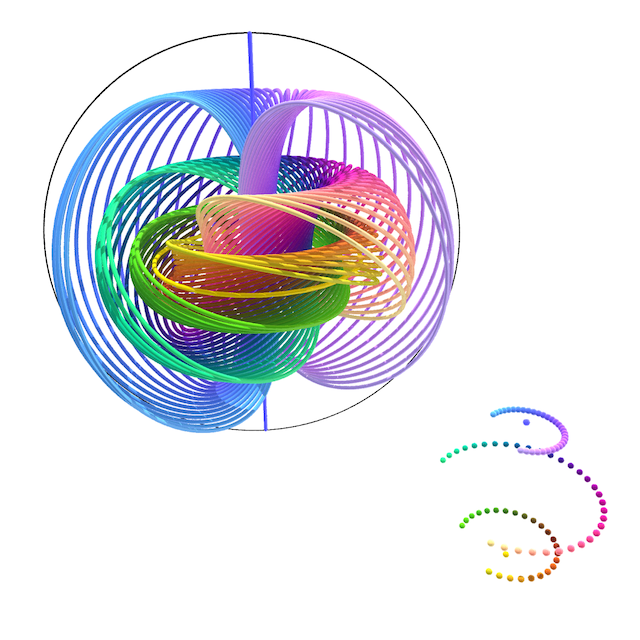
\includegraphics[scale=0.2]{figures/Hopf.png}
        \captionof{figure}{Hopf fibration in stereographic projection, i.e.\ as a fibration of $\bbR^3$. Each circle is a fiber corresponding to a point on the 2-sphere at the bottom. From \cite{hopf}.}
        \label{Fig.Hopf}
    \end{minipage}
\end{example}

\begin{xca}
    Show that in the Hopf bundle, the pre-image of any circle in $\bbS^2$ is a two-torus $\bbT^2$ embedded into $\bbS^3$.
\end{xca}


\begin{defn}[Bundle morphism]\index{Bundle morphism}
    Let $E\overset{\pi}{\to}M$ and $E'\overset{\pi'}{\to}M'$ be two smooth \glspl{fb}. A bundle morphism (a.k.a.\ \emph{bundle map}) between them is a pair of smooth maps $h:E\to E'$ and $\underline{h}:M\to M'$ such that $h$ \emph{covers} $\underline{h}$ in the sense that the following square commutes:
    \[\begin{tikzcd}[every matrix/.append style={name=m},   
    execute at end picture={\draw [<-] ([xshift=-8mm,yshift=1mm]m-2-2.north) arc[start angle=-90,delta angle=270,radius=0.25cm];}]
       E \arrow[r,"h"]\arrow[d,swap,"\pi"]& E'\arrow[d,"\pi'"] \\
       M\arrow[r,swap,"\underline{h}"]& M'
    \end{tikzcd}\]
    We call $\underline{h}$ the \emph{base map}, or the \emph{projection}, of $h$, since it can be uniquely recovered from $h$.\index{Base map}
    This gives rise to the category $\FB^\infty$ of all smooth \glspl{fb}. A full subcategory is the category $\FB^\infty_M$ of all smooth \glspl{fb} over a given base $M$ with $\underline{h}=\id_M$ (note that in general there are other bundle morphisms between bundles over $M$ for which $\underline{h}$ is not even a diffeomorphism). Bundle morphisms covering the identity are also called \emph{vertical}.
\end{defn}








\subsection{Structure groups}\label{sec: structure groups}

So far we have only given a purely topological (or geometric in the smooth case) description of fiber bundles. The fascinating thing about fiber bundles, however, is that the requirement of local triviality gives rise to an alternative \emph{algebraic} description of fiber bundles, which will eventually lead us into the realm of cohomology. A similar, but more cumbersome, description appears for general topological fibrations as well. We now characterize fiber bundles in terms of their systems of local trivializations and identify their transition maps with certain Lie group actions. Note that everything here easily translates to the category of topological fiber bundles as well.


\begin{defn}[Bundle atlas, $G$-structure, cocycle]
    Let $E\overset{\pi}{\to}M$ be a smooth \gls{fb} with typical fiber $F$, and let $\{U_\alpha\}_\alpha$ be an open covering of $M$ such that the restrictions $\restr{E}{U_\alpha}$ are trivial. By definition of local triviality, we have some diffeomorphisms $\chi_\alpha: \restr{E}{U_\alpha}\to U_\alpha\times F$, called \emph{local trivializations}. Then:
\begin{itemize}

    \item The collection $\{(U_\alpha,\chi_\alpha)\}$ is called a \emph{\gls{fb} atlas} for $E\overset{\pi}{\to}M$. Two bundle atlases are \emph{equivalent} if their union is still a bundle atlas. A \emph{bundle structure} on $E$ is an equivalence class of bundle atlases, or, alternatively, a \emph{maximal atlas} given by the union of all atlases belonging to an equivalence class.
    
    \item For any point $(m,f)\in U_{\alpha\beta}\times F$, the transition maps in this atlas have the form \[\chi_\beta\circ\chi_\alpha^{-1} (m,f)=(m, t_{\beta\alpha}(m,f)),\label{eq transition functions}\], 
    where for every fixed $m\in M$, the map $t_{\beta\alpha}(m,\_):F\to F$ is a diffeomorphism. One can think of $t_{\beta\alpha}$ as a function on $U_{\alpha\beta}$ that takes values in the group $\Diff(F)$ of all diffeomorphisms of $F$, so $t_{\beta\alpha}$ becomes a map $t_{\beta\alpha}:U_{\alpha\beta}\to \Diff(F)$.\footnote{As we will see in Section~\ref{sec: Diff groups}, the group $\Diff(F)$ can be given the structure of an infinite-dimensional Lie group, modeled on the space $\fX(F)$ of vector fields. Unfortunately $t_{\alpha\beta}$ are not always automatically smooth: they are smooth iff their values are contained in the left coset of the open and closed subgroup $\Diff_c(F)$ of diffeomorphisms with compact support. This is in principle true only for bundles which are ``trivial near fiber-wise infinity'' or have ``discrete structure group near diberwise infinity'' (see P.W.~Michor ``Gauge theory for diffeomorphism groups'', 1988). We shall always assume that this is true.}
    These $\Diff(F)$-valued functions are called \emph{bundle transition functions}. They are also sometimes called \emph{clutching functions}, especially when $M$ is a sphere.\index{Clutching functions}\index{Transition functions} We will usually assume that $\Diff(F)$ acts on the typical fiber from the \emph{left} (one can pass to a right action by acting via $t_{\alpha\beta}^{-1}$ instead).
    
    \item If the bundle structure of $E$ contains a bundle atlas whose transition functions take values in a Lie subgroup $G<\Diff(F)$,\footnote{We will formalize the concept of Lie subgroups in Section\ref{sec: Lie theory iii}. For now all we need to know is that Lie subgroups are weakly embedded, which means that restricting a smooth map into $\Diff(F)$ whose image lies in $G<\Diff(F)$ in its range produces a smooth map into $G$. In fact, all subgroups of a Lie group are Lie subgroups.} then such an atlas is called a \emph{$G$-atlas} for $E$. Two $G$-atlases are called \emph{$G$-equivalent} if their union is still a $G$-atlas. A $G$-equivalence class of $G$-atlases, or, alternatively, the maximal $G$-atlas equal to their union, is called a \emph{$G$-structure}, denoted $\calG$.\index{$G$-structure} If a $G$-structure is fixed on $E$, we say that $G$ is the \emph{structure group} of the bundle. \index{Structure group} The tuple $(E\overset{\pi}{\to}M,G\acts F,\calG)$ is called a \emph{$G$-bundle}.\index{$G$-bundle}
    
    \item If $H<G$ is a Lie subgroup and a given $G$-structure on $E$ contains an $H$-atlas, then a choice of an $H$-structure (which is a subset of the given $G$-structure) is called a \emph{reduction of the structure group}, or simply a \emph{bundle reduction}\index{Bundle reduction} from $G$ to $H$.
    
    \item From the definition (\ref{eq transition functions}) it is obvious that the group-valued bundle transition functions satisfy two important conditions:
    \[
    \begin{cases}
    t_{\alpha\alpha}\equiv e, & \text{(identity condition),}\\
    \restr{t_{\alpha\beta}\cdot t_{\beta\gamma}\cdot t_{\gamma\alpha}}{U_{\alpha\beta\gamma}}\equiv e; & \text{(cocycle condition),}
    \end{cases}
    \]
    where the product in $\Diff(F)$ is just the composition of maps. Any collection of such $G$-valued functions $\{t_{\alpha\beta}\}$ associated to an open covering of $M$ is called a \emph{cocycle}\index{Cocycle} on $M$ with structure group $G$.\footnote{More precisely, a cocycle is a certain equivalence class of such collections, which is discussed below.} Note that these two conditions imply $t_{\alpha\beta}t_{\beta\alpha}=e$.
\end{itemize}
\end{defn}

\begin{rem}\label{rem: faithful action on F 0}
    \begin{enumerate}
        \item One can try writing down higher-order relations on the transition functions, such as $t_{\alpha\beta}t_{\beta\gamma}t_{\gamma\delta}t_{\delta\alpha}=e$, but all of them follow from the identity and the cocycle conditions. Meanwhile, replacing the cocycle condition with only $t_{\alpha\beta}t_{\beta\gamma}=e$ would've been insufficient because this doesn't imply the higher-order relations.
        \item $\Diff(F)$ acts on $F$ faithfully by definition, therefore the induced action of any subgroup $G<\Diff(F)$ is faithful as well. This is why in the following definitions we will assume a priori that the action of the structure group on the model fiber is faithful. We will further elucidate the importance of faithfulness in Remark~\ref{rem: faithfulness of action on F}.
        \item A fiber bundle $E\to M$ is trivial iff it admits an $\{e\}$-structure. Indeed, if there is a bundle atlas in which all transition functions evaluate to the identity, then all local trivializations agree on the overlaps and hence stitch into a global trivialization.
    \end{enumerate}
\end{rem}


Since the structure group of a bundle acts on its typical fiber $F$, that is, it acts in the local trivializations, it is natural to ask whether this action ``lifts'' to an action on the actual fibers of the bundle itself. Crucially, the answer is no, however the following restricted concept of a $G$-structure does get naturally translated to the fibers.

\begin{defn}[$G$-fiber]
    Let $F$ be a smooth manifold diffeomorphic to a given manifold $F_0$ and let $G$ be a Lie group acting faithfully from the left on $F_0$, so $G$ can be identified with a Lie subgroup of $\Diff(F_0)$. Two diffeomorphisms $\chi_1,\chi_2:F\to F_0$ are called $G$-equivalent if $\chi_2\circ \chi_1^{-1}\in G$. A $G$-equivalence class $\calG_0$ of such diffeomorphisms, i.e.~an orbit of the action of $G$ on $\Diff(F,F_0)$ by compositions $\chi\mapsto g\circ \chi$, is called a fiber $G$-structure on $F$.\footnote{This terminology is not standard. Unfortunately by a $G$-structure on a manifold people usually mean a $G$-structure on its tangent bundle, whereas our definition here refers to a $G$-structure on the bundle consisting of one fiber over a single point, $F\overset{\pi}{\to}\ast$.} The tuple $(F,G\acts F_0,\calG_0)$ is called a $G$-fiber modeled on $F_0$. An element of $\calG_0$ is called a \emph{$G$-frame}, or a frame \emph{compatible} with the $G$-structure.
\end{defn}


\begin{prop}
    If $\pi:E\to M$ is a fiber bundle with structure group $G$ acting on the typical fiber $F$, then each fiber of $E$ naturally carries a fiber $G$-structure and an action of the center $\rmZ(G)$.
\end{prop}
\begin{proof}
    Consider a fiber $E_m=\pi^{-1}(m)$, $m\in M$. The fact that it carries a fiber $G$-structure is obvious because the value of any $G$-valued transition function at a point $m$ is an element of $G$. 
    
    We now show that if $G$ is not abelian, then there is no natural action of $G$ on the fibers, but there is an action of $\rmZ(G)$. By definition of the typical fiber, there is a diffeomorphism $f_\alpha=\restr{\chi_\alpha}{E_m}:E_m\to F$, which is just the restriction of a local trivialization $\chi_\alpha$. By definition of a $G$-structure, there is a smooth (say left) action of $G$ on the typical fiber $F$. Let $f_\beta:E_m\to F$ be the diffeomorphism coming analogously from another compatible local chart. Then $f_\alpha(p)=t^{-1}\cdot f_\beta(p)$ for all $p\in E_m$ for some $t\in G$, and we can compare what the action of an element $g\in G$ translates to in the fiber $E_m$ under these two diffeomorphisms:
    \[f_\alpha^{-1}(g\cdot f_\alpha(p))=f_\beta^{-1}(tgt^{-1} f_\beta(p)).\]
    Since $t$ can range over all of $G$ by varying the charts, these formulas consistently define an action $g\cdot p$ only for $g\in \rmZ(G)$.
\end{proof}

\begin{rem}
    \begin{enumerate}
        \item The intuition behind the definition of $G$-structures is the following. A fiber $G$-structure on $F$ is a choice of a $G$-invariant subset of all diffeomorphisms from $F$ to a ``standard'' or ``model'' space $F_0$, namely an orbit of the action of $G$ on all such diffeomorphisms by compositions. This can be interpreted as $F_0$ having some kind of ``structure'' that is invariant under actions of $G$, and a fiber $G$-structure allows us to transplant this structure to $F$. A $G$-structure on a fiber bundle, then, is a collection of structures on each fiber that, in a sense, vary smoothly with the base point $m\in M$. These structures are defined consistently because all local trivializations belonging to the same $G$-bundle atlas differ from each other by an action of $G$ on $F_0$, hence this additional structure is independent of the local bundle chart. 
        \item Morphisms between bundles with the same structure group are also defined so as to ``respect'' this structure. Thus the smaller the $G$, the more structure the morphisms of this category preserve. We will use this rough idea when introducing vector bundles, orientations, and complex bundles. For example, vector bundles will have group structure $\GL(V)$ for some vector space $V$, and, as we will see, the corresponding fiber $G$-structure is the structure of vector space.
        
        \item There is one extremely special class of $G$-bundles that will be distinguished by the fact that their typical fiber supports \emph{two} commuting actions of $G$, a left one and a right one (because the typical fiber will be $G$ itself). After using one of them up to define the bundle, we will be able to use the above procedure to lift the other one to a global action of $G$ on $E$. These bundles are called \emph{principal}. In Section~\ref{sec: free proper actions} we will show that principal $G$-bundles can be defined without reference to local trivializations, and in Section~\ref{sec: principal bundles} that will lead us to a chart-free definition of \emph{all} fiber bundles.
    \end{enumerate}
\end{rem}
\begin{example}
    A covering space $E\overset{\pi}{\to} M$ is a topological fiber bundle with a discrete typical fiber $F$. Its structure group, most generally, is the group $G=\Diff(F)=\mathrm{Bij}(F)$ of all permutations of points of the fiber. As we know, there is a natural $\pi_1(M,x_0)$-action on $F=\pi^{-1}(x_0)$, which produces a homomorphism $\lambda:\pi_1(M,x_0)\to G$. Note that there is no natural action of $\pi_1(M,x_0)$ on \emph{other} fibers of $E$ because there is no natural way to choose the isomorphisms between the groups $\pi_1(M,x_0)$ for different choices of the basepoint $x_0$. The image of $\lambda$ is a subgroup of $G$. Since the covering space can be fully reconstructed from this action, $\lambda(\pi_1(M,x_0))$ can be made the structure group of this bundle. 
    
    One case where there is a global action of the structure group on the whole covering space is when it is a $G$-principal covering space. In this case the fiber is $G$ itself and supports a second (right) action of $G$ which survives the fiber bundle construction.
\end{example}






\subsection{Fiber morphisms}\label{sec: fiber morphisms}

Now we examine morphisms (and in particular isomorphisms) between bundles with different structures on them. General bundle morphisms are allowed to be arbitrary smooth maps when restricted to a single fiber, so we will need to find a special subclass of bundle morphisms that ``respects'' given structures in some way. Let us first look at the simpler case of a single fiber. Say we have a $G$-fiber $(F,G\acts F_0,\calG_0)$ and a $G'$-fiber $(F',G'\acts F_0',\calG_0')$. Then any map $h:F\to F'$ can be represented by a map $\wh{h}:F_0\to F_0'$ by using any two diffeomorphisms $\chi\in\calG_0\subset \Diff(F,F_0)$ and $\chi'\in\calG_0'\subset \Diff(F',F_0')$ as follows:
\[\wh{h}=\chi'\circ h\circ \chi^{-1}.\label{eq g-fiber f-hat}\]
Different choices of $\chi$ and $\chi'$ are equivalent to replacing $\wh{h}$ in this formula with $g'\circ \wh{h}\circ g^{-1}$ for some $(g,g')\in G\times G'$. Therefore we notice the importance of the action of the product group $G\times G'$ on the set $C^\infty(F_0,F_0')$ by compositions:
\[G\times G'\acts C^\infty(F_0,F_0'):\quad ((g,g'),\wh{h})\mapsto g'\circ \wh{h}\circ g^{-1}.\label{eq gg' action}\] 
A choice of a class of morphisms $\wt h$ then corresponds to a choice of a set of orbits of this action. For this we either need $F_0$ and $F_0'$ to carry additional structure (vector spaces, metric spaces, etc.) that provides such a choice in a canonical way, or to just specify the choice manually. If want to make these choices consistently across all possible pairs of model spaces $(F_0,F_0')$, this amounts to forming a category. We detail these methods below:
\begin{enumerate}
    \item Let $\calS$ be a subcategory of the category $\mathsf{Man}^\infty$ of smooth manifolds (it need not include neither all objects nor all morphisms). Then if the model spaces $F_0$ and $F_0'$ are objects of $\calS$, we denote
    \[\calS(F_0,F_0')=\mor_\calS(F_0,F_0').\]
    We think of the category $\calS$ as describing ``additional structure'' on the model spaces. We now define morphisms from $(F,G\acts F_0,\calG_0)$ to $(F',G'\acts F_0',\calG_0')$ as maps $h:F\to F'$ which, under some (and therefore any) diffeomorphisms $\chi\in\calG_0$ and $\chi'\in\calG_0'$, are represented by maps $\wh{h}:F_0\to F_0'$ belonging to $(G\times G')\cdot \calS(F_0,F_0')$.
    
    \item In the situation of item 1, it is also often the case that $G$ and $G'$ \emph{act by automorphisms}, i.e.\ by elements of $\Aut_\calS(F_0)$ and $\Aut_\calS(F_0')$, respectively. Then 
    \[(G\times G')\cdot \calS(F_0,F_0')=\calS(F_0,F_0').\]
    This situation comes with an extra benefit. Since $G$ preserves the additional structure on $F_0$, this structure can be ``lifted'' via any $\chi\in \calG_0$ so that $F$ itself naturally becomes an object of $\calS$. Thus, in addition to the action of $\rmZ(G)$, the fiber will inherit some additional structure from the $G$-invariant structure on the model fiber. We will soon see how this works explicitly on the example of vector bundles.
    \item The most common setting is a special sub-case of 2, whereby $G$ and $G'$ are \emph{defined} as the groups of automorphisms of $F_0$ and $F_0'$, respectively, so we don't even need to specify them separately:
    \[G=\Aut_\calS(F_0),\quad G'=\Aut_\calS(F_0').\]
    The actions of $G$ and $G'$ in this case are given canonically, and we can proceed as in 1. In particular, this implies that every representative $\wh{h}$ of every \emph{automorphism} (invertible morphism of a $G$-fiber to itself) $h$ is an element of $G$.
\end{enumerate}

\begin{defn}[Category of $\calS$-fibers]\label{def S-fibers}
    Given a $G$-fiber $(F,G\acts F_0,\calG_0)$, a $G'$-fiber $(F',G'\acts F_0',\calG_0')$, and a subset $\calS(F_0,F_0')\subset C^\infty(F_0,F_0')$ determined from a category $\calS$ in one of the ways described above, a morphism between them is a smooth map $h: F\to F'$ such that its representative $\wh{h}$ defined by (\ref{eq g-fiber f-hat}) using any $\chi\in\calG_0$ and $\chi'\in\calG_0'$ belongs to the orbit of an element of $\calS(F_0,F_0')$ under the action (\ref{eq gg' action}) of $G\times G'$ on $C^\infty(F_0,F_0')$. We say that $h$ \emph{is modeled on} an element of $\calS(F,F')$. We call this category $\calS\mathsf{-Man}^\infty$ and its objects $\calS$-fibers. Note that $\calS$ is not enough to define this category -- one also needs to specify groups $G$ and their actions (unless $G=\Aut(F_0)$ as in case 3 above).

    In particular, two $G$-fibers $(F,G\acts F_0,\calG_0)$ and $(F',F\acts F_0,\calG_0')$ with the same structure group $G$ and model space $F_0$ are isomorphic if and only if there exists a diffeomorphism $h:F\to F'$ such that the map $\calG_0'\to \calG_0$ given by the composition $\chi'\mapsto h^\ast \chi'=\chi'\circ h$ is a bijection. If $G=\Aut_\calS(F_0)$, then this is equivalent to $\wh{h}\in G$ for all representatives (\ref{eq g-fiber f-hat}) of $h$.
\end{defn}

Note that the choice of the category $\calS$ for a given type of structure is not unique. In fact we mostly need this definition to produce a unique notion of \emph{isomorphism} of $\calS$-fibers and later $\calS$-bundles, whereas we won't really care what the rest of the morphisms look like. We now consider a number of important examples of $\calS$-fiber structures.
\begin{example}[Linear $G$-structures]\label{ex linear G-structures}
    \begin{enumerate}
        \item If $\calS=\mathsf{FinVect}_\bbK$ (finite-dimensional $\bbK$-vector spaces), then we get the category of $\mathsf{FinVect}_\bbK$-fibers with linear maps. Here, if the model space is $V$, then we define $G=\Aut_\calS(V)=\GL(V)$. A $G$-structure $\calG_0$ on $F$ is an equivalence class of diffeomorphisms $F\to V$ that differ by an automorphism of $V$. Since $V$ is a vector space, we can use any of these diffeomorphisms $\chi\in\calG_0$ to induce a vector space structure on $F$ itself: for $\lambda_1,\lambda_2\in\bbK$ and $e_1,e_2\in F$ we define the linear combination
        \[\lambda_1e_1+\lambda_2 e_2\coloneqq \chi^{-1}(\lambda_1\chi(e_1)+\lambda_2\chi(e_2)).\]
        This is well-defined because different $\chi$'s differ by a linear automorphism of $V$. In particular, this defines an action of scalar matrices $\lambda I$, $\lambda\in\bbK$, on $F$, which coincides with the induced natural action of the center $\rmZ(G)$. Note that $\GL(V)$ has no natural action on $F$ because there is no natural isomorphism between $F$ and $V$! Thus the category $\calS\mathsf{-Fib}$ is isomorphic to $\calS$ itself.

        In fact, one can replace the category $\mathsf{FinVect}_\bbK$ with its skeleton $\mathsf{Sk}(\mathsf{FinVect}_\bbK)$, whose objects are \emph{standard} spaces $\bbK^n$, $n=0,1,\ldots$, and the only nontrivial morphisms are inclusions-as or projections-onto the first $n$ components. Indeed, every linear map between vector spaces is represented by one of these standard maps in some appropriately chosen bases of the source and target spaces. In this case an element of $\calG_0$, i.e.\ a \emph{frame}, determines a basis on $F$ and outputs the components of vectors in that basis.
        
        \item In general, if structure groups $G$ are defined as the automorphism groups $\Aut(F_0)$, then the resulting category $\calS\mathsf{-Fib}$ is equivalent to $\calS$ itself. This allows one to define many classical structures on vector spaces in terms of a countable set of ``standard'' ones. This shows the importance of allowing $G$ to not necessarily act by automorphisms. We proceed in this manner in the next several examples.
        
        \item If $\bbK=\bbR,\bbC,\bbH$, then we can let $\calS$ be the category of finite-dimensional vector spaces with a $\bbK$-valued dot product, or its skeleton consisting of spaces $\bbK^n$ with the standard dot product $\sum_{i=1}^n \wb{x}_i y_i$. For each model space $\bbK^n$ we also take its isometry group $G$, which is $\Or_n,\U_n$, or $\Sp_n$, respectively. Then $\calS$-fibers are vector spaces $F$ with a $G$-structure which allows us to lift the dot product onto $F$. There is a bijective correspondence between $G$-structures and dot products on $F$, so  $\calS\mathsf{-Fib}$ is exactly the category of vector spaces with a dot product and all linear maps. $G$-frames in this context are just orthonormal bases. We can also replace $\calS$ with the category of vector spaces $V$ with a dot product and linear morphisms whose operator norm is at most $1$ (this forces isomorphisms to be isometries), and letting $G=\Aut_\calS(V)$. Then $\calS\mathsf{-Fib}$ has the same objects but fewer morphisms.

        \item If we let $\calS=\mathsf{FinVect}_\bbK$ but redefine the structure group $G$ of a model space $V$ as $G=\GL^+(V)$, i.e.\ orientation-preserving automorphisms, then $\calS$-fibers are oriented vector spaces with linear maps between them. 

        \item If $\calS$ is again the category of standard real vector spaces $\bbR^n$, $n=0,1,\ldots$, and the structure group of $\bbR^n$ is $\SL_n(\bbR)$, then $\calS$-fibers are vector spaces with a volume form (a totally antisymmetric multilinear form of maximum rank) with linear maps between them. Alternatively we can let $\calS$ consist of $\bbR^n$'s with the standard volume form $\mathsf{v}_n$ and linear maps $f:\bbK^n\to \bbK^m$ such that $f^\ast \mathsf{v}_m=\lambda \mathsf{v}_n$ with $\lambda\in (-1,1]$ (this forces automorphisms to have determinant $1$), and define $G=\Aut_\calS(\bbR^n)\cong \SL_n(\bbR)$. Note that a volume form induces an orientation because $\SL_n(\bbR)\subset \GL_n^+(\bbR)$.

        \item Taking standard model spaces $\bbK^n$ with $G$ defined as the group that leaves the subspace $\bbK^p$ spanned by the first $p$ standard basis vectors, and linear maps that map the first $p$ directions of one space to the first $p$ directions of the other (not necessarily surjectively), we get the category $\calS\mathsf{-Fib}$ of vector spaces with ``$p$-directions''. It is isomorphic to the category of pairs $(V,W)$ where $W$ is a $p$-dimensional subspace of $V$, and morphisms are required to be maps of pairs (i.e.\ $W$ is mapped inside $W'$). Note that morphisms between standard spaces $\bbR^n\to \bbR^m$ are represented by matrices with the top right $p\times(n-p)$ block filled with zeroes (unless $p>m$, in which case it's just the right $m\times (n-p)$ block).

        \item Consider all free actions of the group $G=\GL_n(\bbZ)$ on $n$-dimensional vector spaces $V$. This means that $G$ is the group of linear automorphisms of $V$ that preserve some rank-$n$ lattice $\Lambda$ spanning $V$ (i.e.\ $\Lambda=\bbZ v_1+\cdots +\bbZ v_n$ for some basis $v_1,\ldots,v_n$). Then $\calS\mathsf{-Fib}$ is the category of vector spaces with an \emph{integral affine structure}. It is isomorphic to the category of pairs $(V,\Lambda)$ and linear maps mapping lattice to lattice.

        \item $\calS$ be the category of even-dimensional real vector spaces $V$ with a linear isomorphism $\sfJ:V\to V$ such that $\sfJ^2=-\id_V$ and linear maps $h:(V,\sfJ)\to(V',\sfJ')$ such that $h\circ \sfJ=\sfJ'\circ h$. Each $\sfJ$ defines a complex structure on $V$ by $\rmi v\coloneqq\sfJ(v)$. Then $G=\Aut_\calS(V)$ consists of matrices $A\in\GL(V)$ such that $\sfJ A=A\sfJ$ and is isomorphic to $\GL_n(\bbC)$ (exercise). $\calS\mathsf{-Fib}$ is isomorphic to $\calS$ itself and is the category of complex structures on real vector spaces with complex-linear maps between them. $\calS$ can also be replaced with its skeleton, which consists of standard complex structures on $\bbR^{2n}$:
        \[\rmJ_{2n}=\begin{bmatrix}
            0&-\rmI_n\\
            \rmI_n&0
        \end{bmatrix}\]
        And linear maps $f:\bbR^{2n}\to \bbR^{2m}$ that satisfy $\rmJ_{2m}\circ f=f\circ \rmJ_{2n}$. In the case $m=n$ such maps are called holomorphic and their matrices have the form 
        \[M=\begin{bmatrix}
            A&B\\
            -B&A
        \end{bmatrix},\label{eq complex matrices}\]
        which can be identified with $A+\rmi B\in \Mat_n(\bbC)$.
        Note that each complex structure also induces an orientation because matrices $A\in \GL_n(\bbC)\subset \GL_{2n}(\bbR)$ have positive determinant over $\bbR$, namely $\det M=|\det(A+\rmi B)|^2>0$.

        \item Consider standard spaces $\bbR^{2n}$ with standard symplectic forms, i.e.\ antisymmetric nondegenrate bilinear forms $\omega_{2n}:\bbR^{2n}\times \bbR^{2n}\to \bbR$ whose matrix in the standard basis is $\rmJ_{2n}$. Let morphisms be all linear maps and let $G=\Sp_{2n}(\bbR)$ be the group of symplectic matrices, i.e.\ matrices $A\in\GL_{2n}(\bbR)$ such that $A^T\rmJ_{2n}A=\rmJ_{2n}$. Then $\calS$-fibers are symplectic vector spaces $(V,\omega)$ with all linear maps between them. This can be reduced to just the category of \emph{symplectomorphisms}, i.e.\ isomorphisms that preserve the symplectic structure.
    \end{enumerate}
\end{example}


\begin{example}[Hermitian structures]\label{ex hermitian structures}
    A Hermitian structure on a complex vector space $V_\bbC$ is just a symmetric sesquilinear form $\sfh:V_\bbC\times V_\bbC\to \bbC$ as introduced in example 2, i.e.
    \[h(v,w)=\widebar{h(w,v)},\quad v,w\in V_\bbC,\]
    and $h(v,v)\geq 0$ for all $v\in V_\bbC$ and vanishes iff $v=0$.
    
    An $n$-dimensional complex vector space is naturally isomorphic to a $2n$-dimensional real vector space with a complex structure $V_\bbC\cong (V,\sfJ)$ (defined by $\sfJ(v)\coloneqq \rmi v$), also denoted $V_\sfJ$. Then $\sfh$ can be reinterpreted as a complex-valued $\bbR$-bilinear form on $V_\sfJ$ which in addition satisfies
    \[\sfh(v,\sfJ w)=-\sfh(\sfJ v,w)=\rmi\sfh(v,w),\quad v,w\in V_\sfJ,\]
    and such that $\sfh(v,v)$ is a norm. This also implies that
    \[\sfh(\sfJ v,\sfJ w)=\sfh(v,w).\]
    We can decompose $\sfh$ into its real and imaginary parts, which we suggestively call $\sfg$ and $\omega$:
    \[\sfh(v,w)=\Re \sfh(v,w)+\rmi\Im\sfh(v,w)=\sfg(v,w)+\rmi \omega(v,w).\]
    We have
    \[\sfg(v,w)=\Re \sfh(v,w)=\Re \sfh(w,v)=\sfg(w,v),\]
    and $\sfg(v,v)=\sfh(v,v)$, therefore $\sfg$ is a nondegenerate symmetric bilinear form that defines a dot product on $V_\sfJ$.
    Furthermore, the sesquilinear condition implies that 
    $\omega(v,w)=\frac12 (\rmi\sfh(w,v)-\rmi\sfh(v,w))=\frac12 (\sfh(w,\sfJ v)-\sfh(v,\sfJ w))$
    is a real antisymmetric bilinear form. 
    Moreover,
    \[\omega(v,\sfJ w)=\frac12 (\sfh(\sfJ w,\sfJ v)+\sfh(v,w))=\frac12 (\sfh(w,v)+\sfh(v,w))=\Re \sfh(v,w)=\sfg(v,w),\]
    therefore $\omega$ is nondegenerate as well, and hence determines a symplectic structure on $V_\sfJ$. 

    Crucially, fixing a complex structure $\sfJ$, the above formulas relating any two of the three objects $\sfh,\sfg,\omega$ uniquely determine the third. We thus have natural isomorphisms between the following three pairs of structures:
    \begin{enumerate}
        \item Hermitian structures $(\sfJ,\sfh)$ on $V$.
        \item Pairs $(\sfJ,\sfg)$ of a complex structure $\sfJ$ and a metric $\sfg$ that are compatible in the sense that
        \[\sfg(\sfJ v,\sfJ w)=\sfg(v,w),\quad \text{or}\quad \sfg(\sfJ v,w)=-\sfg(v,\sfJ w),\quad v,w\in V.\]
        This compatibility condition is equivalent to the bilinear form $\omega_\sfJ(v,w)=\sfg(\sfJ v,w)$ being a symplectic form, also called the \emph{fundamental form}.
        \item Pairs $(\sfJ,\omega)$ of a complex structure $\sfJ$ and a symplectic structure $\omega$ that are compatible in the sense that
        \[\omega(\sfJ v,\sfJ w)=\omega(v,w),\quad \text{or}\quad \omega(\sfJ v,w)=-\omega(v,\sfJ w),\quad v,w\in V,\]
        and in addition that the resulting form $\sfg_\sfJ(v,w)=\omega(v,\sfJ w)$, which is symmetric because of compatibility, is positive definite (in this case we say that $J$ \emph{tames} $\omega$). These conditions are equivalent to the bilinear form $\sfg_\sfJ$ being a real scalar product.
        \item Pairs $(\sfg,\omega)$ of a positive definite metric $\sfg$ and a symplectic form $\omega$. By non-degeneracy of $\sfg$, there exists a unique operator $\sfJ$ such that $\omega(v,w)=\sfg(v,\sfJ w)$, and it follows that $\sfJ$ is a complex structure compatible with both $\sfg$ and $\omega$.
    \end{enumerate}
    Thus the group of isometries of $\sfh$, $\U(V,\sfh)$, coincides with the following double intersections of groups $\Sp(V,\omega)$ (automorphisms preserving $\omega$), $\GL(V_\bbC)$ (automorphisms preserving $\sfJ$), and $\Or(V,\sfg)$ (automorphisms preserving $\sfg$):
    \[\U(V,\sfh)=\Sp(V,\omega)\cap \GL(V_\bbC)=\Or(V,\sfg)\cap \GL(V_\bbC)=\Or(V,\sfg)\cap \Sp(V,\omega).\]
    In particular, for standard model spaces $(\bbR^{2n},\rmJ_{2n})$ we get the \emph{``2 out of 3 property of unitary groups''}:
    \[\U_n=\Sp_n(\bbR)\cap \GL_n(\bbC)=\Or_{2n}\cap \GL_n(\bbC)=\Or_{2n}\cap \Sp_n(\bbR),\]
    which is also obvious from the fact that any two of the defining equations $A^T\sfJ A=\sfJ$, $A^{-1}\sfJ A= \sfJ$, $A^TA=I$, imply the third.
    Here, $\GL_n(\bbC)$ is included in $\GL_{2n}(\bbR)$ as the set of invertible matrices of the form (\ref{eq complex matrices}) identified with $A+\rmi B\in \GL_n(\bbC)$.
    
    The triple $(\sfJ,\sfg,\omega)$ consisting of compatible complex, metric, and symplectic structures on $V$ can be called a \emph{linear K\"ahler structure}.\index{K\"ahler structure} As we have seen, the set of K\"ahler structure is bijective with the set of Hermitian structures, which is why in the linear case the term K\"ahler structure is redundant.
\end{example}

\begin{xca}
    \begin{enumerate}
        \item Show that the space of metrics on a vector space is convex, i.e.\ for any two metrics $\sfg_1$ and $\sfg_2$, all bilinear forms $t\sfg_1+(1-t)\sfg_2$, $t\in[0,1]$, are also metrics. Hence it is contractible.
        \item Show that the space of Hermitian forms $\sfh$ is also convex and hence contractible.
        \item Show that the set $\calJ(V,\omega)\subset \GL(V)$ of complex structures compatible with a given symplectic form $\omega$ (but not necessarily taming it) is contractible. See \cite[Prop.~7.5.7]{RS1}.
    \end{enumerate}
\end{xca}







\subsection{Bundle morphisms}

Now we extend our definition of morphisms to arbitrary \glspl{fb}. Consider a morphism $h:E\to E'$ between two arbitrary bundles $E\overset{\pi}{\to}M$ and $E'\overset{\pi'}{\to}M'$ with potentially differing structure groups $G$ and $G'$. Pick local trivializations $\{(U_\alpha,\chi_\alpha)\}_{\alpha\in A}$, $\{(U_a',\chi_a')\}_{a\in A'}$ on the two bundles with corresponding cocycles $\{t_{\alpha\beta}\}$ and $\{t_{ab}'\}$ and denote $U_{\alpha a}=U_\alpha\cap \underline{h}^{-1}(U_a')$. Then the bundle morphism is locally represented by maps
$\wh{h}_{\alpha a}:U_{\alpha a}\times F\to F'$ as follows: 
\[\boxed{h\left(\chi_\alpha^{-1}(m,f)\right)=\chi_a^{\prime-1}\left(\underline{h}(m),\wh{h}_{\alpha a}(m,f)\right).}\label{eq def of hab}\]
By transforming to other local charts $\chi_\beta$ and $\chi_b'$ via formula (\ref{eq transition functions}) we have
\[h\left(\chi_\beta^{-1}(m,t_{\beta\alpha}(m)\cdot f)\right)=\chi_b^{\prime-1}\left(\underline{h}(m),t_{ba}'(\underline{h}(m))\cdot\wh{h}_{\alpha a}(m,f)\right).\]
On the other hand, (\ref{eq def of hab}) written for $\wh{h}_{\beta b}$ implies
\[h\left(\chi_\beta^{-1}(m,t_{\beta\alpha}(m)\cdot f)\right)=\chi_b^{\prime-1}\left(\underline{h}(m),\wh{h}_{\beta b}\left(m,t_{\beta\alpha}(m)\cdot f\right)\right).\]
By comparing the right hand sides of the last two formulas and using the fact that $\chi_b'$ is a fiberwise diffeomorphism, we conclude that
\[\boxed{\wh{h}_{\beta b}\left(m,t_{\beta\alpha}(m)\cdot f\right)=t_{ba}'(\underline{h}(m))\cdot \wh{h}_{\alpha a}(m,f).}\label{eq transformation of hab}.\]
This is a complicated condition on the collection of maps $\{\wh{h}_{\alpha a}\}$ with respect two different cocycles. Despite this condition these maps can still look like completely arbitrary smooth maps when restricted to a single fiber. However, in many cases we would like to consider only those bundle morphisms which, in some sense, respect the given group structures. To this end, consider the set of smooth maps $C^\infty(F,F')$ (which is an infinite-dimensional smooth manifold) and the left action of $G\times G'$ on it by compositions:
\[(G\times G')\acts C^\infty(F,F'):\quad ((g,g'),\varphi)\mapsto g'\circ \varphi\circ g^{-1}.\]
Then every $\hat{h}_{\alpha a}:U_{\alpha a}\times F\to F'$ can be used to define a fiberwise $G\times G'$-equivariant map
\begin{gather}
    \Phi_{\alpha a}: U_{\alpha a}\times (G\times G')\to C^\infty(F,F'),\\
    (m,(g,g'))\mapsto \left(f\mapsto g'\cdot \hat{h}_{\alpha a}\left(\underline{h}(m),g^{-1}\cdot f\right)\right).\label{def Phiab}
\end{gather}
It is easy to see that this map is $G\times G'$-equivariant (with $G\times G'$ acting on itself from the left). Moreover, every fiberwise $G\times G'$-equivariant map arises this way ($\hat{h}_{\alpha a}$ can be recovered by substituting $g=g'=e$), although the correspondence of course is not bijective.\footnote{Note how the fact that $\Phi_{\alpha a}$ are defined on sets of the form $U_{\alpha a}\times (G\times G')$ hints that they themselves represent a function defined globally on some fiber bundle with typical fiber $G\times G'$. We will return to this in our discussion of principal bundles.} The transformation rule (\ref{eq transformation of hab}) now becomes
\[\boxed{\Phi_{\beta b}(m,g,g')=\Phi_{\alpha a}\left(m,gt_{\beta\alpha}(m),g't_{ba}'(\underline{h}(m))\right).}\label{eq transformation of Phiab}\]
We would like to put some restriction on the values of these maps in $C^\infty(F,F')$ that produces a well-defined class of bundle morphisms $\wt h$ which can be interpreted as ``respecting'' the given $G$- and $G'$-structures. This can be easily done by analogy with how we interpreted the structure of a $G$-fiber:
\begin{gather}
    \text{All maps }\{\Phi_{\alpha a}\}_{\alpha\in A,a\in A'}\text{ should be required to take values}\\
    \text{in a single orbit of the }G\times G'\text{-action on }C^\infty(F,F').
\end{gather}
This is a well-defined constraint because, due to the equivariance of $\Phi_{\alpha a}$, the transformation law (\ref{eq transformation of Phiab}) implies that the fiber above $p$ gets mapped to the same orbit regardless of the values of the indices $\alpha,a$.

\begin{defn}[Category ${\calS \mFB}^\infty$]\label{def S-bundle}
    Let the objects of the category $\calS\mFB^\infty$, called $\calS$-bundles, be all possible structured bundles $(E\overset{\pi}{\to}M,G\acts F,\calG)$ with model fibers $F\in\ob(\calS)$ and with sets of maps $\calS(F,F')\subset C^\infty(F,F')$ determined from a category $\calS$. Morphisms from such a bundle to another one, $(E'\overset{\pi'}{\to}M',G'\acts F',\calG')$, are bundle morphisms $h:E\to E'$ such that $\calG$ and $\calG'$ contain some $G$- and $G'$-atlas, respectively, in which $h$ is represented by a collection of $G\times G'$-equivariant maps $\{\Phi_{\alpha a}\}$ as above which satisfy the compatibility condition (\ref{eq transformation of Phiab}) and which take values in the orbit of a single element of $\calS(F,F')$ under the action of $G\times G'$ on the set $C^\infty(F,F')$. We say that $h$ \emph{is modeled on} an element of $\calS(F,F')$.

    In addition, ${\calS\mFB}_M^\infty$ is the subcategory of structured bundles over the fixed base manifold $M$ with morphisms covering the identity in $M$, i.e.\ we assume $h=\id_M$.
\end{defn}

There are a number of other subcategories one may define by additionally either fixing the fiber, the structure group, or both. The most important subcategory for us will be the following.

\begin{defn}[Category $\FB^\sigma$]\label{def FB^sigma}
    The category $\FB^\sigma$ consists of so called $(G,\sigma)$-bundles with a fixed structure group $G$, typical fiber $F$, and faithful action $\sigma:G\times F\to F$. The morphisms are required to be such that their local representatives lie in the orbit of the identity map on $F$. That is, locally morphisms are represented simply by actions of elements of $G$ on $F$.
\end{defn}


\begin{example}
    Consider the cylinder $E=\bbS^1\times\bbR $ as a line bundle over the circle. We can trivialize it with all transition functions being the identity. In the category of all line bundles (with structure group $\Diff(\bbR )$) there is a bundle map $E\to E$ that maps $(p,x)\mapsto (p,-x)$. However, in the category of bundles with the trivial structure group $G=\{e\}$ (i.e.\ the category of trivial bundles) this is not an allowed bundle map because it does not act trivially on the fiber.
\end{example}


\begin{defn}[Bundle construction]\label{def bundle construction}
    \Glspl{fb} can be alternatively defined by specifying the base manifold $M$, the typical fiber $F$, the structure group $G$ acting on the fiber via a \emph{faithful}\footnote{The importance of faithfulness will be explained in Remark~\ref{rem: faithfulness of action on F}.} smooth left action which can be viewed as an injective homomorphism of Lie groups $\Phi:G\to \Diff(F)$ (i.e.\ we will write $g\cdot f=\Phi(g)(f)=\Phi_g(p)$ for $g\in G, f\in F$), a countable open covering $\{U_\alpha\}$ of $M$, and a cocycle  $t_{\beta\alpha}\in C^\infty (U_{\alpha\beta}, G)$. Namely, we can define $E$ as a topological space as the quotient $E\coloneqq \bigslant{(\bigsqcup_\alpha U_\alpha \times F)}{\sim}$, where $(m_1,f_1)\sim(m_2,f_2)$ iff $m_1=m_2=m$ and $f_1=t_{\beta\alpha}(m,f_2)$ for some $\alpha,\beta$, and the projection $\pi$ is defined as the descendent of the projections onto the fist component in each summand.\footnote{In categorical terms, this is literally the cofibered product (pushout) of the sets $U_\alpha \times F$ with pairs of maps $\restr{\chi_\alpha^{-1}}{U_{\alpha\beta}\times F}$ and $\restr{\chi_\beta^{-1}}{U_{\alpha\beta}\times F}$. For instance, if there were only two sets $U_1,U_2$, we would have $E=(U_1\times F)\sqcup_Z (U_2\times F)$, where $Z=U_{12}\times F$ and we have two morphisms $\restr{\chi_i^{-1}}{U_{12}\times F}:Z\to U_i\times F$ that are used in the definition of the pushout.}
    Then $E$ has a unique smooth structure that makes $\pi$ a smooth submersion (see \cite[Lem.~10.6]{Lee} for the case of vector bundles, which is easily generalized to all \glspl{fb}).\footnote{Essentially we can take an atlas $\{F_\alpha,\psi_\alpha\}$ of $F$ and an atlas $\varphi_\alpha$ of $M$ (\gls{wlog} subordinate to the covering $\{U_\alpha\}$) to construct a smooth atlas $\{(U_\alpha\times F_\beta,\varphi_\alpha\times\psi_\beta)\}$ of $E$.} This construction is called the \emph{clutching construction} of a \gls{fb}.
\end{defn}


The fact that any $(G,\sigma)$-bundle over $M$ can be uniquely reconstructed from a $G$-valued cocycle on $M$ means that this category doesn't really depend on the fiber $F$ and the action $\sigma$ very much. Namely, for any other faithful $G$-action $\sigma':G\times F'\to F'$ there is an equivalence of categories
\[C_{\sigma',\sigma}:\FB^\sigma\to \FB^{\sigma'}.\label{eq equivalence of bundle categories}\]
The functors going in either direction take a bundle, choose a cocycle for it, and then construct the other bundle using the same cocycle via the other action. Faithfulness of the actions is clearly necessary for this to be an equivalence of categories because only then are the cocycles uniquely defined. The key insight flowing from this equivalence is that, to study arbitrary fiber bundles, it will suffice to pick one particular kind of typical fibers and group actions on them which makes computations easy. This computationally convenient class of bundles turns out to be the class of \emph{principal bundles}, where the typical fiber coincides with the structure group. We discuss them in the examples below.



\begin{example}[Linear $G$-structures on manifolds]
    \begin{enumerate}
        \item Regardless of $\calS$, if $G=\{e\}$, then a $G=\{e\}$-structure is equivalent to a global trivialization of the bundle. In the case of vector bundles, this is called an \emph{absolute parallelism}.\index{Parallelism!absolute}
        \item $\calS=\mathsf{FinVect}_\bbR$, and the structure group of each vector space $F$ is $\GL(V)$, then $\calS$-bundles are just vector bundles. Each fiber is naturally an $\calS$-fiber, i.e.\ a vector space, and vector bundle morphisms are exacly fiberwise linear bundle morphisms.
        \item A $\GL_k^+$-structure on a vector bundle of rank $k$ is called an orientation because it selects an orientation on every fiber in a continuous fashion. A vector bundle that admits such a structure is called \emph{orientable}.\index{Orientable vector bundle}
        \item An $\Or_k$-structure on a vector bundle $E$ of rank $k$ is equivalent to a smooth choice of metrics $\sfg_m$ on each fiber $E_m$. In Section~\ref{sec: Riemannian mfds} we will see that every real manifold admits such a choice, called a \emph{Riemannian structure}, so every vector bundle admits a (non-unique) reduction of the structure group to an orthogonal group. $\Or_k$-bundles are known as \emph{Riemannian bundles}. This fact is equivalent to the statement that $\GL_k(\bbR)$ deformation retracts onto $\Or_n$. In addition, if the bundle is orientable, the structure group can be reduced to $\SO_n$.
        \item A $\GL_k(\bbC)$-structure on a real vector bundle $E$ of rank $2k$ is equivalent to a smooth choice of complex structures $\sfJ_m$ on each fiber $E_m$. Such bundles are called \emph{complex vector bundles} of rank $k$. Every complex vector bundle is oriented.
        \item A $\Sp_{2k}(\bbR)$-structure on a (real) vector bundle $E$ of rank $2k$ is equivalent to a smooth choice of symplectic forms $\omega_m$ on each fiber $E_m$. If such a choice exists, we get a \emph{symplectic vector bundle}.
        \item A $\U_k(\bbR)$-structure on a rank $k$ complex vector bundle is a smooth choice of a Hermitian dot product on each fiber. As we will see, every complex vector bundle admits such a choice, thus any $\GL_k(\bbC)$-structure can be reduced to a $\U_k$-structure. Note that a further reduction to $\SU_k$ is not always possible, and its existence doesn't have a standard name (we will later see that it is equivalent to the triviality of the determinant line bundle $\det E$, or to the vanishing of the first Chern class, $c_1(E)=0$).
    \end{enumerate}
    Note that every one of these structures, just like in the linear case, defines a canonical choice of frames (bases) in each fiber, and via local trivializations they can be chosen smoothly over an open subset of the base. 
\end{example}

\begin{example}[Nonlinear $G$-bundles]
    \begin{enumerate}
        \item If $\calS=\mathsf{LieGr}$ with the structure group of each Lie group $G$ being its automorphism group $\Aut(G)$, then $\calS$-bundles are what is called \emph{group bundles}. Since automorphisms preserve the identity and the rest of the group structure, each fiber of a group bundle carries a natural Lie group structure. In particular, each group bundle has one canonical section $\sigma_e:M\to E$ whose value in each fiber is the identity element of that fiber.\index{Group bundle}
        
        \item If $\calS=\mathsf{LieGr}$ but with the structure group of a Lie group $G$ being $G$ itself acting by left translations, then we get what are called \emph{principal bundles} and they are so important that we shall put off a detailed discussion of them until Section~\ref{sec: principal bundles}. For now we only note the crucial difference between group and principal bundles: the fibers of a principal $G$-bundle, despite being diffeomorphic to $G$, are not Lie groups since left translations don't preserve the identity element.\index{Principal fiber bundle} This is another important example where the group action on the typical fiber falls outside of the set of morphisms allowed by the category $\calS$.
    \end{enumerate}
\end{example}

The following theorem is one of the most important theorems for the applications of fiber bundle theory, for example in complex-analytic problems of differential equations (where it is known as the Riemann-Hilbert factorization problem).

\begin{thm}\label{bundle isomorphism thm}
Two $G$-bundles $E$ and $E'$ over $M$ are isomorphic iff there exists a covering $\{U_\alpha \}$ of $M$, two corresponding cocycles $\{t_{\alpha\beta}\}$ and $\{t_{\alpha\beta}'\}$, and a set of $G$-valued functions $\lambda_\alpha:U_\alpha\to G$ such that $t_{\alpha\beta}'(p)\equiv \lambda_\alpha (p) t_{\alpha\beta}(p) \lambda_\beta^{-1}(p)$ for all $p\in U_{\alpha\beta}$. In particular, a bundle is trivial iff its transition functions can be factorized as $t_{\alpha\beta}=\lambda_\alpha \lambda_\beta^{-1}$.
\end{thm}
\begin{proof}
Given two bundle atlases over $M$, we can always take all possible pairwise intersections of the sets of the two covers of $M$ to refine the atlases so that they are defined over the same covering of $M$. \gls{wlog}, any isomorphism of bundles over the same base can be assumed be identity on the base itself (e.g. because if the horizontal part of the isomorphism is some diffeo $f:M\to M$, we can replace one of the bundles by the isomorphic pullback bundle along $f$, see Definition~\ref{Pullback bundle}). Then from (\ref{eq transformation of hab}) we see that any bundle isomophism gives rise to the $\lambda_\alpha$'s, and vice versa, $\lambda_\alpha$'s completely describe the bundle isomorphism. 
\end{proof}
\begin{defn}[Equivalent cocycles]
    Two $G$-valued cocycles on $M$ that are related (after being brought over to a common set of charts $\{U_\alpha\}$) by the above formulas for some collection of maps $\lambda_\alpha:U_\alpha\to G$ are called \emph{$G$-equivalent}. The equivalence class $[\{t_{\beta\alpha}\}]$ itself is also called a cocycle.
\end{defn}
\begin{cor}
    Given a manifold $M$ and a faithful smooth action $G\overset{\sigma}{\acts} F$, there is a bijective correspondence between isomorphism classes of $(G,\sigma)$-bundles over $M$ and ($G$-equivalence classes of) $G$-valued cocycles on $M$.
\end{cor}
This correspondence can actually be restated as an equivalence of the category $\FB^\sigma$ and a certain category of cocycles.

\begin{rem}\label{rem: faithfulness of action on F}
    Faithfulness of the action is crucial here. As we noted in Remark~\ref{rem: faithful action on F 0}, any structure group whose action is induced from the action of $\Diff(F)$ acts on $F$ faithfully. We can see the importance of this property when recostructing a bundle from a cocycle acting on a model fiber. If, for example, $F$ is a single point, then every group action on $F$ is trivial and there is only one fiber bundle over $M$ with fiber $F$ regardless of the structure group $G$, whereas there are still many non-equivalent $G$-valued cocycles on $M$. Therefore faithfulness is needed so that the cocycle is well-defined in this sense. In the future we will run into important situation where, for instance, $F$ is a finite-dimensional vector space with an action of a non-linear group $G$ (namely a spin group), so that this action cannot be faithful, and thus the correspondence with classes of cocycles will not be one-to-one.
\end{rem}






\subsection{Flat bundles}

Now let us try to use this transformation rule for transition functions to ``simplify'' the cocycle and see how far we can go. If we have two charts with a transition function $t_{\alpha\beta}$, then we always find a pair of functions $\lambda_\alpha,\lambda_\beta$ on those charts such that $\lambda_\alpha t_{\alpha\beta}\lambda_\beta^{-1}$ is constant, in fact equal to identity: just pick $\lambda_\alpha=e$ and let $\lambda_\beta$ be an arbitrary smooth extension of $t_{\alpha\beta}$ from $U_{\alpha\beta}$ to all of $U_\beta$. We can try to keep expanding this procedure to more and more charts, but there is no guarantee that we will be able to make all transition functions constant. Thus we single out the following important class of bundles.

\begin{defn}[Flat $G$-structure]\index{Flat!fiber bundle}\index{Flat!$G$-structure}
	A $G$-structure on a \gls{fb} is called \emph{flat} if it contains a bundle atlas with constant (or locally constant) transition functions. Alternatively, a $G$-structure is flat if structure group $G$ can be reduced to a subgroup with a \emph{totally disconnected} topology (one where all connected subsets are one-point sets, e.g.\ the discrete topology; then the transition functions are forced to be constant by continuity). If the default $\Diff(F)$-structure is flat, then the bundle itself is called flat.
\end{defn}
\begin{rem}
    Note that the flatness of the bundle (with respect to the default $\Diff(F)$-structure) does not imply that all other $G$-structures on it are flat.
\end{rem}


\begin{example}[Line bundles above $\bbS^1$]\label{line bundles over S1}
    We can use the idea of a bundle atlas and Theorem \ref{bundle isomorphism thm} to classify all line bundles above the circle up to isomorphisms. It suffices to pick one covering of the circle, so we will pick a covering by the three circular arcs $U_1=(\epsilon,4\pi/3-\epsilon)$, $U_2=(2\pi/3+\epsilon,2\pi-\epsilon)$, and $U_3=(4\pi/3+\epsilon,8\pi/3-\epsilon)$. The transition functions in a line bundle take values in the group $G$ of diffeomorphisms of $\bbR $. Each such diffeomorphism is a smooth function $f:\bbR \to\bbR $ such that $f'$ is never zero. Now, clearly $G$ consists of two path-connected components, one of diffeomorphisms that preserve the orientation, i.e.\ $f'(x)>0$ for all $x$, and others that reverse it, $f'(x)<0$. We say that these diffeomorphisms have one of two possible \emph{parities}. Let $g_+(x)=\id_{\bbR }(x)=x$ and $g_-(x)=-x$, so that $g_+$ is the identity element of $\Diff(\bbR )$ and $g_-$ is an orientation-reversing involution.

    There are three transition functions, $t_{12}$, $t_{23}$, and $t_{31}$. Any three $G$-valued functions $\lambda_1,\lambda_2,\lambda_3$ provide an isomorphic line bundle. Choose $\lambda_1\equiv g_+$. Furthermore, $t_{12}:U_{12}\to G$ can be extended to a continuous function $\lambda_2: U_2\to G$, $\restr{\lambda_2}{U_{12}}=t_{12}$. Then $t_{12}'=\lambda_1 t_{12}\lambda_2^{-1}\equiv g_+$. By continuity, all values of $\lambda_2$ have the same parity.  Now, we let $\lambda_3$ be a continuous extension to $U_3$ of the function $\lambda_2 t_{23}:U_{23}\to G$. Then $t_{23}'=\lambda_2 t_{23} \lambda_3^{-1}\equiv g_+$. Finally, $t_{31}'=\lambda_3 t_{31} \lambda_1=\lambda_3 t_{31}$.  The parity of the values of $t_{31}'$ by construction is the product of the parities of $t_{12}$, $t_{23}$, and $t_{31}$.

    The values of $\lambda_3$ are already uniquely fixed up to the point $2\pi-\epsilon=-\epsilon$. Due to the path-connectedness of the two components of $G$, $\lambda_3$ can be deformed on $U_3\setminus U_{23}=(-\epsilon,2\pi/3-\epsilon)$ so that it remains smooth and $\restr{\lambda_3}{(\epsilon,2\pi/3-\epsilon)}=g_\pm t_{31}^{-1}$, which leads to $t_{31}'\equiv g_\pm$.

    This means that any line bundle above $\bbS^1$ is isomorphic to one of two bundles, whose transition functions are either all identities, or one of them is a reflection $x\mapsto -x$.  In other words, any line bundle over $\bbS^1$ can be reduced to the structure group $O(1)=\bbZ_2$. The former bundle is trivial, and the latter bundle is homeomorphic to the M\"obius band. There are only two isomorphism classes of line bundles above $\bbS^1$.
\end{example}

\begin{xca}\label{Rk-bundles above circle}
    Show that if $f:\bbR^K\to \bbR^k$ is a diffeomorphism such that $f(0)=0$, then $f_t(x)=f(tx)/t$ is a homotopy from $f$ to an element of $\GL_k(\bbR)$. Use this to argue that the group $\Diff(\bbR^k)$ has only two path-connected components, and that there are only two isomorphism classes of \glspl{fb} with fiber $\bbR^k$  above $\bbS^1$ for any $k$.
\end{xca}
\begin{xca}
    Show that every diffeomorphism of the circle $\bbS^1\subset \bbC$ is homotopic to one of the two maps $z\mapsto z^{\pm 1}$. Using this fact, classify all circle bundles over $\bbS^1$ (i.e.~with typical fiber $\bbS^1$). Note that this result can also be obtained from Exercise~\ref{Rk-bundles above circle}.
\end{xca}

\begin{example}
    Staying in the category of topological fiber bundles, let us classify two-fold covering spaces of the ``figure eight space'' in the language of fiber bundles. The fiber $F$ in this case consists of two points. The base space $M=\bbS^1\vee \bbS^1$ can be covered by three contractible sets: one $\mathsf{x}$ and two intervals. All of their overlaps are contractible, and therefore by adjusting the transition functions we will always be able to make them constant. This we have four overlaps with four corresponding elements of the structure group $G=S_2$. The bundle will be constructed out of the disjoint union of two copies of each of our three pieces: we need to glue the following six pieces $\begin{matrix}
        |\; \times \;|\\
        |\; \times \;|
    \end{matrix}$. Now note that two of the transition functions, namely one on the left side of the base manifold $\infty$ and one on the right, can be turned into the identity by permuting the two pairs of straight segments to match those two permutations. Thus we end up with two copies of $\infty$, where each loop has been cut at one point, giving us two pairs of cuts to glue back using the two permutations. Since each permutation can only take two values, we get a total of four covering spaces. Two of them happen to be isomorphic if we allow for nontrivial diffeomorphisms of the base (the left-right symmetry of $\infty$), but usually the classification is done without considering such symmetries. One of the fiber bundles obtained this way is trivial, and the other three are represented in Figure \ref{fig:coverings of 8}(1,2).
\end{example}

The following example is a preview of the concept of connection, which will be the main subject of \Part~\ref{Part Structured Geom}. It can be safely skipped without loss of continuity.

\begin{example}[Covering spaces and flat bundles with flat connections]
	Covering spaces are just \glspl{fb} with discrete fibers, therefore their structure group $G$ is the permutation group of the points of the typical fiber. The classification theorem for covering spaces stated that all bundles over $M$ with the discrete fiber $F$ are classified by all possible homomorphisms $\pi_1(M)\to G$ (up to global conjugation by an element of $G$ corresponding to a shuffling of the points of $F$). Therefore, up to the fact that the action of $\pi_1(M)$ is often not faithful, we can say that the structure group of any covering space over $M$ is $\pi_1(M)$.
	
	Continuing Remark~\ref{covering spaces and connections}, we see that the monodromy, or holonomy, is also nothing but a representation of $\pi_1(M)$ on the fiber. Therefore bundles with discrete fibers are completely classified by the monodromy/holonomy of the connection on them. Can we generalize these ideas to a larger class of bundles?
	
	First of all, by a simple extension of the argument in Example \ref{line bundles over S1}, we see  that all bundles with fiber $F$ and structure group $G$ above $\bbS^1$ are classified by homomorphisms $\Hom(\pi_1(M),\pi_0(G))/\sim$, where $\pi_0(G)=G/G_0$ and $G_0$ is the connected component of the identity in $G$ (which is a normal subgroup), so that $\pi_0(G)$ is the group whose elements are the connected components of $G$. The equivalence relation is the global conjugation of all values of the given homomorphism by an arbitrary element of the target group (corresponds to a diffeomorphism on $F$, which of course doesn't change the bundle). For instance, for $F=\bbR $ and $G=\Diff(\bbR )$, we found that $\pi_0(G)=\bbZ_2$. The statement also agrees with the classification theorem for covering spaces.
	
	Recall that a connection is just a prescription for lifting curves from the base into the total space. The lifted curves are called \emph{horizontal}, and the lifting procedure is also known as \emph{parallel transport} (of the starting point in the bundle along the path in the base). If the curve in the base is a loop $\gamma$ such that $\gamma(0)=\gamma(1)=p\in M$, then its lifts with all possible starting points $\wt{\gamma}(0)=e_0\in E_p$ determine the holonomy $e_0\mapsto e_1=\wt{\gamma}(1)=h(\gamma)(e_0)$, where we introduced the map $h:\gamma\mapsto h(\gamma)\in G$. Defined this way, $h(\gamma)$ is an element of the structure group $G$, and moreover $h$ is a homomorphism from the group $L_p(M)$ of all loops based at $p$ to $G$. The image of this homomorphism is a subgroup $\mathrm{Hol}_p<G$ called the \emph{holonomy group} of the bundle based at $p$. If $h$ is restricted only to contractible loops, then the corresponding group is called $\widetilde{\mathrm{Hol}}_p<\mathrm{Hol}_p<G$, the \emph{local holonomy} group at $p$. 
	
	If $\widetilde{\mathrm{Hol}}_p=\{\id\}$ for all $p$, the connection is called \emph{flat}. This is equivalent to the property that the holonomy depends only on the homotopy class of the base loop. In particular, a small simply connected neighborhood $U\subset M$ of $p\in M$ can be uniquely lifted to a local section of $E$ passing through $e_0\in E_p$, which is of course diffeomorphic to $U$. That is, $E$ can be locally fibrated by horizontal sections, each diffeomorphic to $U$. 
	
	Flatness of a connection is sometimes called \emph{integrability}\index{Integrability}, and is exactly what people mean when they speak of integrable systems in physics: the phase space of an integrable system can be fibrated by hypersurfaces that are locally spanned by physical trajectories.
	
	Finally, we notice that the definition of flat \glspl{fb} given above implies the existence of a flat connection. Namely, a loop $\gamma$ in $M$ that passes through charts $U_1,U_2,\ldots,U_n=U_1$ with the starting point $(p,f)\in U_1\times F$ can be lifted as $(\gamma(t),f)$ on $U_1$, $(\gamma(t),\tau_{21}f)$ on $U_2$, $(\gamma(t),\tau_{32}\tau_{21}f)$ on $U_3$, and so on (here $\tau_{ij}\in G$ represent the constant transition functions). These actually stitch together into a continuous path under the identifications in the bundle. Similarly one can lift non-closed curves, which completes the definition of the connection.
	
	Exercise: check that the local holonomy of the connection just described is independent of the choice of a bundle atlas (even though the connection itself does depend on the atlas) and trivial , i.e.\ the connection is indeed flat.
	
	The non-local part of the holonomy is described by ordered products of transition functions $\prod \tau_{ij}$ along non-contractible loops. Since these are homotopy-invariant, we have a homomorphism $\pi_1(M)\to G$ that completely describes the holonomy of the flat connection. A global conjugation $g\mapsto g_0 g g_0^{-1}$ on the group doesn't affect the connection (it is essentially equivalent to shifting the base point in the definition of $\pi_1(M)$), therefore all flat connections on bundles with structure group $G$ above $M$ are classified by $\Hom(\pi_1(M),G)/\sim$, where $\sim$ is the conjugation equivalence. Moreover, one can show that every homomorphism of this kind corresponds to a bundle with a connection. This is the generalization of the classification theorem for covering spaces.
	
	Note that a flat bundle with structure group $G$ and a flat connection is the same as a fiber bundle whose structure group is $G$ with the discrete topology (because in the latter situation the transition functions as well as all deformation parameters $\lambda_\alpha$ are forced to be constant functions, the flat connection is unique and given by the construction above). All this leads us to conclude that flat bundles with a flat connection, or bundles with totally disconnected structure groups, are the natural generalization of covering spaces.
	
	We have shown that bundles over $M$ with a totally disconnected structure group $G$ are precisely classified by the conjugacy classes of homomorphisms $\Hom(\pi_1(M),G)$. The conjugacy class of such homomorphisms corresponding to a bundle $E\overset{\pi}{\to}M$ is called the \emph{characteristic class}\index{Characteristic class} of the bundle. Therefore, for totally disconnected structure groups, a single characteristic class determines the isomorphism class of the bundle.
	
	The main goal for Parts \ref{Part II} and \ref{Part III} of these lectures will be to develop the machinery necessary for the full classification of \glspl{fb} with arbitrary topological structure groups, in particular by extending the theory of characteristic classes. The characteristic class we have just constructed (acting on one-dimensional cycles, i.e.\ closed loops) is only the first one in an infinite list of cohomology classes corresponding to a given bundle.
\end{example}

\begin{comment}
    \begin{samepage}
        \PRLsep
        \begin{center}
            {\red Lecture 9 on 25 Jan 2019 ended here}
        \end{center}
    \end{samepage}
\end{comment}








\subsection{Subbundles, pullbacks}


We've seen that bundles are, in categorical terms, pushouts (i.e.\ quotients of disjoint unions) of a family of trivial bundles along the trivialization maps. The categorical notion of pullback introduced in Definition \ref{pullbacks} is also very useful in the theory of \glspl{fb}.

\begin{defn}[Pullback bundle]\index{Pullback bundle}\label{Pullback bundle}
    Let $E\overset{\pi}{\to}M$ be a smooth \gls{fb} and $N\overset{f}{\to}M$ a smooth map. We define the \emph{pullback of $E$ along $f$}, or the bundle \emph{induced from $E$ by $f$}, denoted $f^\ast E$, in three ways:
    \begin{itemize}        
        \item $f^\ast E=\{(n,p)\in N\times E\mid f(n)=\pi(p)\}\subset E\times N$ with the subspace topology induced from $E\times N$. Obviously we have two canonical projections onto the two components of the product, $f^\ast E\overset{\wt{f}}{\to}E$ and $f^\ast E\overset{\pi'}{\to}N$. The latter one is the new bundle projection, equal to the restriction of the natural projection $\pr_1$ on $N\times E$. We show below that there is a unique smooth structure on $f^\ast E$ that makes $\pi'$ into a smooth submersion.
        \item If the typical fiber of $E$ is $F$ and we know a set of transition functions $t_{\alpha\beta}:U_{\alpha\beta}\to G$ defining $E$, then $f^\ast E$ can be defined as the bundle with base $N$, same fiber $F$, and transition functions $f^\ast t_{\alpha\beta}:f^{-1}(U_{\alpha\beta})\to G$, where $f^\ast t\coloneqq t\circ f$ is the definition of the \emph{pullback of a function} $t$ on $M$ via $f$.
        \item In categorical terms, it is literally the pullback $N\times_M E$ that uses the maps $E\overset{\pi}{\to}M$ and $N\overset{f}{\to}M$ in its Cartesian square. This object indeed exists because it can be explicitly constructed using either of the next two alternative definitions. The pullback naturally comes with two canonical projections $f^\ast E\overset{\wt{f}}{\to}E$ and $f^\ast E\overset{\pi'}{\to}N$.
    \end{itemize} 
    \[\begin{tikzcd}[every matrix/.append style={name=m},   
    execute at end picture={\draw [<-] ([xshift=-8mm,yshift=1mm]m-2-2.north) arc[start angle=-90,delta angle=270,radius=0.25cm];}]
   f^\ast E \arrow[r,"\wt{f}"]\arrow[d,swap,"\pi'"]& E\arrow[d,"\pi"] \\
   N\arrow[r,swap,"f"]& M
    \end{tikzcd}\label{eq pullback bundle diagram}\]
\end{defn}

\begin{lem}[{{\cite[Prop.~1.7.3, Rem.~1.7.4]{RS1}}}]\label{prop 1.7.3 RS1}
    Let $N$ be a smooth manifold and $M\subset N$ a subset with the relative topology induced from $N$. Consider the following condition.
    \begin{enumerate}[label=(E)]
        \item \begin{enumerate}[label=(E\alph*)]
            \item $M\subset \bigcup_i V_i$,
            \item for every $i$, $V_i\cap M$ admits a smooth structure of dimension $l$ with respect to which it is an embedded submanifold of $N$.
        \end{enumerate}
    \end{enumerate}
    If condition (E) holds for some $l\in\bbN$, the smooth structures on $V_i\cap M$ induce a smooth structure on $M$, with respect to which $M$ is an embedded submanifold of $N$. Conversely, if there exists a smooth structure on $M$ which makes it an embedded submanifold of dimension $l$, then (E) holds for this $l$ and the induced smooth structure on $M$ coincides with the original one.
\end{lem}
\begin{proof}
    Pick local slice charts $(V_i,\rho_i)$ on $N$ such that $\rho(V_i\cap M)=\rho_i(V_i)\cap (\bbR^l\times \{0\})$. As a topological subspace of $N$, $M$ is Hausdorff and second countable. For every $i$, $V_i\cap M$ is open in the relative topology. Being the restriction of a homeomorphism onto its image, $\restr{\rho_i}{V_i\cap M}$ is a homeomorphism onto its image. Since by assumption the image is $\rho_i(V_i)\cap (\bbR^l\times\{0\})$ and is hence open in $\bbR^l\times\{0\}$, these data give a local chart on $M$. The transition maps are obtained by restriction of the original local charts on $N$ to subsets of the subspace $\bbR^l\times\{0\}$ which are open by condition (E2). Hence the transition maps are smooth and define a smooth structure. By definition of the relative topology the inclusion is open onto its image, thus $M$ is embedded.
\end{proof}


\begin{prop}[{{\cite[Prop.~2.6.1]{RS1}}}]\label{prop 2.6.1 RS1}
\begin{enumerate}
    \item $f^\ast E$ defined via any of the first two definitions has a unique smooth structure that turns the bundle projection into a smooth submersion.
    \item All three definitions are isomorphic as smooth bundles.
    \item $f^\ast E$, defined as in the first definition, is in fact an embedded submanifold of $N\times E$.
\end{enumerate} 
\end{prop}
\begin{proof}
    We apply Lemma~\ref{prop 1.7.3 RS1}. Choose a typical fiber $F$ and a system of local trivializations $\{(U_\alpha,\chi_\alpha)\}$ for $E$. For every $\alpha$ consider the open subset $V_\alpha=f^{-1}(U_\alpha)$ of $N$ and the mapping  
    \[\psi_\alpha:V_\alpha\times F\to N\times E,\quad \psi_\alpha(m,u)=(m,\chi_\alpha^{-1}(f(m),u)).\]
    Since $\psi_\alpha$ is obtained by composing the diffeomorphism $\chi_\alpha^{-1}$ with the natural inclusion mapping of the graph of $\restr{f}{V_\alpha}:V_\alpha\to U_\alpha$, it is a smooth embedding (see Example~\ref{example submanifolds}). Hence the image $\psi_\alpha(V_\alpha\times F)$ inherits a smooth structure from $V_\alpha\times F$ with respect to which it is an embedded submanifold of $N\times E$. Since the image is $f^\ast E\cap (V_\alpha\times\pi^{-1}(U_\alpha))$ and since the $V_\alpha\times\pi^{-1}(U_\alpha)$ are open subsets of $N\times E$ covering $f^\ast E$, we conclude that $f^\ast E$ is an embedded submanifold. This proves assertion 3, and Lemma~\ref{prop 1.7.3 RS1} also shows the uniqueness of this smooth structure, proving assertion 1. Assertion 2 is an exercise.
\end{proof}

\begin{xca}[Pullback of a bundle by itself]
    Given the $n$-fold covering of the circle $\bbS^1\overset{\pi}{\to}\bbS^1$, show that the pullback $\pi^\ast \bbS^1=\bbS^1\times_{\bbS^1} \bbS^1$ is a trivial fiber bundle over $\bbS^1$. As we will see later, this is a general fact about \emph{principal} fiber bundles.
\end{xca}

\begin{rem}
\begin{enumerate}
    \item From the proof of Proposition~\ref{prop 2.6.1 RS1}, every local trivialization of $E$ induces a local trivialization of $f^\ast E$. In particular, the pullback of a trivial bundle is trivial. As indicated above, transition functions also get simply pulled back by $f^\ast \tau_{\alpha\beta}=\tau_{\alpha\beta}\circ f$.
    \item A bundle morphism $h:E'\to E$ covering a map $\underline{h}:M'\to M$ naturally decomposes as
    \[E'\overset{h_{\mathrm{ver}}}{\to} \underline{h}^\ast E\overset{h_{\mathrm{hor}}}{\to} E,\label{eq 2.6.2 RS1}\]
    where $h_{\mathrm{ver}}(x)=(\pi'(x),h(x))$, $x\in E'$, and $h_{\mathrm{hor}}=\underline{\wt{h}}$ is the induced vector bundle morphism $\wt{f}$ defined by the pullback diagram (\ref{eq pullback bundle diagram}) for $f=\underline{h}$. One can check that $h_{\mathrm{ver}}$ is a vertical bundle morphism.  Using this decomposition, one can give the following characterization of isomorphisms in terms of their projections and fiber mappings: a bundle morphism is an isomorphism iff its projection (the base map) is a diffeomorphism and its fiber mappings are bijective.
\end{enumerate}
\end{rem}


\begin{defn}[Restriction of a bundle]\index{Restriction of a fiber bundle}
    If $S< M$ is a submanifold via an immersion $i:S\to M$ and $E\overset{\pi}{\to}M$ is a smooth \gls{fb}, then we can define the restricted bundle $\restr{E}{S}\coloneqq i^\ast E$. It is a smooth \gls{fb} by the last proposition.
\end{defn}

\begin{defn}[Spaces of sections]\index{Section of a fiber bundle}
    A smooth section of a smooth \gls{fb} $E\overset{\pi}{\to}M$ is a smooth map $\sigma:M\to E$ such that $\pi\circ \sigma=\id_M$. The space of all sections, with the compact-open topology, is denoted $\Gamma^\infty_M(E)$. If $U\subset M$ is an open subset, or more generally an immersed submanifold, then a \emph{local section} over $U$ is a section of the restricted bundle $\restr{E}{U}$, and the space of all local sections over $U$ is denoted $\Gamma^\infty_U(E)=\Gamma^\infty(\restr{E}{U})$.
\end{defn}
\begin{rem}
    It is not in general true that every local section can be realized as a restriction of a global section. For example, the two-fold cover of the circle $\bbS^1\to \bbS^1$ has no global sections at all. More broadly, the properties of bundles that prevent an extension of local structures to global ones are called \emph{obstructions}. The obstructions to the existence of global sections turn out to be of purely algebraic-topological nature and are described by cohomology, as we will see in Part~\ref{Part III}.
\end{rem}


\begin{xca}\label{example 2.7.3 RS1}
\begin{enumerate}
    \item Show that if $E$ is trivial, then $f^\ast E$ is trivial for any $f$. In other words, pullbacks of bundles are always ``at least as trivial'' as the original bundles.
    \item Show that if $(\wt{f},f)$ is a bundle map from $E$ to $E'$ that is also a fiberwise diffeomorphism, then $E\cong f^\ast E'$.
    \item Show that if $S<M$ is immersed, weakly embedded, or embedded, then $\restr{E}{S}$ is respectively an immersed, weakly embedded, or embedded, subbundle of $E$. See \cite[Example~2.7.3]{RS1}.
\end{enumerate}
\end{xca}



\begin{prop}
    Let $E\overset{\pi}{\to}M$ be a smooth \gls{fb} and let $\sigma:M\to E$ be a section (i.e.~a smooth map such that $\pi\circ\sigma=\id_M$). Then $(M,\sigma)$ is an embedded submanifold of $E$.
\end{prop}
\begin{proof}
    It suffices to show that there exists an open neighborhood $V$ of $\sigma(m)$ in $E$ such that $(\sigma^{-1}(V),\restr{\sigma}{\sigma^{-1}(V)})$ is an embedded submanifold. Since local trivializations are diffeomorphisms, this follows from the fact that the graph of any smooth map $\psi:M\to N$ is an embedded submanifold of $M\times N$.
\end{proof}



\begin{defn}[Fiber subbundle]\index{Fiber subbundle}
    A (immersed, weakly embedded, or embedded) subbundle of a smooth \gls{fb} $E\overset{\pi}{\to}M$ is a \gls{fb} $E'\overset{\pi'}{\to}M'$ with an injective \gls{fb} morphism $\wt{h}:E'\to E$ which turns $E'$ into an immersed, weakly embedded, or embedded, respectively, submanifold of $E$. If $M=M'$ then we usually assume that $\wt{h}$ covers the identity in the base, and we call such subbundles \emph{vertical}, or \emph{subbundles over $M$}. 
\end{defn}

\begin{prop}[{{\cite[Prop.~2.7.4]{RS1}}}]
    Consider a bundle morphism $H:E'\to E$ covering a map $h:M'\to M$.  \gls{tfae}:
    \begin{enumerate}
        \item $(E',H)$ is a subbundle (resp.~immersed, weakly embedded, embedded) of $E$.
        \item $(M',h)$ is a submanifold (resp.~immersed, weakly embedded, embedded) of $M$ and the fiber maps $H_m:E'_m\to E_m$ are injective for all $m\in M'$.
        \item In the decomposition (\ref{eq 2.6.2 RS1}), $(E',H_{\mathrm{ver}})$ is a vertical subbundle of $h^\ast E$ and $(h^\ast E,H_{\mathrm{hor}})$ is a subbundle (resp.~immersed, weakly embedded, embedded) of $E$.
    \end{enumerate}
\end{prop}
\begin{proof}
    $1\Rightarrow 2$ The fiber maps $H_m$ are obviously injective. Since Since all bundles have local sections, let $\sigma':U'\to E'$ be such a local section for $E'$. Then $H\circ\sigma'$ is a smooth local section over the set $h(U')$ (which may not be open) for $E$. Every local section over an open set is an embedding, in particular $\sigma'$, and thus its composition with another submanifold map, $H\circ \sigma'$, defines a submanifold of $E$ of the same type as $H$. This submanifold is the image of a section of $\pi$, and $\pi$ restricted to any section is a diffeomorphism onto the domain of that section. Thus the composition $\pi\circ H\circ \sigma':U'\to h(U')$ is also a submanifold of the same type. Finally, since $\pi$ is locally trivial, this means that every point $m\in M$ has a neighborhood $U$ such that $h(M')\cap U$ coincides with a submanifold of the form we described above. This implies that the entire image $h(M)$ is a submanifold.
    
    $2\Rightarrow 3$ Since the $H_m$ are injective, $H_{\mathrm{ver}}$ is injective, hence the assertion on $(E',H_{\mathrm{ver}})$ holds since every vertical subbundle is embedded. The assertion on $(h^\ast E,H_{\mathrm{hor}})$ was proven in Exercise~\ref{example 2.7.3 RS1}.

    $3\Rightarrow 1$ Since vertical subbundles are embedded, this follows from transitivity of submanifold properties as earlier in this proof.
\end{proof}




\subsection{Homotopy invariance}


\begin{thm}[Bundles over $M\times I$ {{\cite[Thm.~3.3.1]{RS2}}}]\label{bundles over MxI}
    Every \gls{fb} $E$ over $M\times I$, where $I=[0,1]$, is isomorphic to $E_0\times I$ where $E_0=\restr{E}{M\times\{0\}}$. The isomorphism can be chosen so that its restriction to $E_0$ is the inclusion $E_0\hookrightarrow E\times I$ as $p_0\mapsto (p_0,0)$.
\end{thm}
\begin{proof}
    First we show that $E$ can be trivialized over a locally finite open covering of the form $\{U_i\times I\}_i$.

    By local triviality, for a fixed $x\in M$ and every $t\in I$, there is an open neighborhood $V_t\subset M$ of $x$ and an open interval $t\in I_t\subset I$ such that $E$ is trivial over $V_t\times I_t$. Therefore we can construct a countable, locally finite open covering of $M\times I$ with sets of this kind. By compactness, there is a finite set $0<t_1<\cdots<t_k<1$ such that $\bigcup_i I_{t_i}=I$. Let $V_i=V_{t_i}$, $I_i=I_{t_i}$, and define 
    \[
        U_i=\bigcap_{j=1}^i V_j,\quad J_i=\bigcup_{j=1}^i I_j.
    \]
    Obviously $E$ is trivial over $U_1\times J_1$. Let $\chi_1$ be a trivialization of $E$ over $U_1\times J_1$ and $\wt{\chi}_2$ -- one over $V_2\times I_2$. Then $(U_1\times J_1)\cap (V_2\times I_2)=U_2\times (J_1\cap I_2)$. Assuming that $I_2$ intersects $J_1$ non-trivially and one is not contained in the other (otherwise $I_2$ can be dropped from the covering of $I$), consider the transition function $\tau:U_2\times(J_1\cap I_2)\to G$ defined by $\chi_1(p)=\left(\id\times    \tau(\pi(p))\right)\cdot \wt{\chi}_2(p)$. Choose $c\in J_1\cap I_2$ and a continuous function $f:I_2\to J_1\cap I_2$ such that $f(t)=t$ for $t\geq c$ to define 
    \[
        \wt{\tau}:U_2\times I_2\to G,\quad \wt{\tau}(x,t)=\tau(x,f(t)).
    \]
    Clearly $\tau$ and $\wt{\tau}$ coincide on $U_2\times([0,c]\cap I_2)$. Hence the new mapping
    \[
    \chi_2(p)=\begin{cases}
    \chi_1(p), & \pi(p)\in U_2\times[0,c],\\
    (\id\times\wt{\tau}(\pi(p)))\cdot \wt{\chi}_2(p), & \pi(p)\in U_2\times I_2
    \end{cases}
    \]
    defines a trivialization of $E$ over $U_2\times I_2$. By induction, we find that $E$ is trivial over every every $U_i\times I$. 

    We sketch the rest of the proof. Since this construction applies to every $x\in M$, we can extract a locally finite open covering of the entire $M$ of the form $\{U_i\times I\}_i$ such that $E$ is trivial over every set in the covering (this can be done using a \gls{pou}). Let $\chi_i$ be the corresponding local trivializations and $\wh{\chi}_i$ the induced local trivializations of $\restr{E_0}{U_i}\times I$.

    Now we construct a global trivialization inductively in $i$. For $V_1=U_1$, there is already an isomorphism $\Phi_1:\restr{E}{V_1\times I}\to\restr{E_0}{V_1}\times I$. We can construct a chain of open sets $V_1\subset V_2\subset\cdots$ that eventually covers all of $M$ and $U_i\subset V_i$, and by induction extend the isomorphism to $\Phi_i:\restr{E}{V_i\times I}\to\restr{E_0}{V_i}\times I$. Via the local trivializations $\chi_i$ and $\wh{\chi}_i$, bundle isomorphisms are represented by $G$-valued functions $g_i:U_{i}\times I\to G$ with $g_i(x,0)=e\in G$. Let $g_1:(V_1\cap U_2)\times I\to G$ be the representative of $\Phi_1$ in $\chi_2$ and $\wh{\chi}_2$. Then $g_1$ can be smoothly extended to $V_2\times I$ so that it equals $e$ on $(U_2\setminus V_1)\times I$. This represents the isomorphism $\Phi_2$ that agrees with $\Phi_1$ on the common domain. Repeating this procedure on $U_3$ and so on, we construct a global isomorphism of the bundles in question. See \cite[Thm.~3.3.1]{RS2} for details.
\end{proof}

\begin{cor}
    Continuous deformations (homotopies) of transition functions within the class of cocycles don't change the isomorphism class of a fiber bundle.
\end{cor}



Therefore, in the most general and abstract sense, the ``full'' characteristic class\index{Characteristic class} of a fiber bundle (which uniquely classifies the bundle) is the ``conjugacy'' and homotopy equivalence class of cocycles for it.

Now we are ready to prove the smooth version of the \gls{hlp} for fiber bundles (a continuous version of it holds automatically since every smooth fiber bundle is a Hurewicz fibration).

\begin{thm}[Homotopy Lifting Property/Covering Homotopy Theorem]\label{HLP}
    Let $E\overset{\pi}{\to}M$ and $E'\overset{\pi'}{\to}M'$ be smooth \glspl{fb} with the same typical fiber $F$. If $(\wt{H}_0,H_0)$ is a bundle map from $E$ to $E'$ and $H:M\times I\to M'$ is a homotopy of $H_0$, i.e.\ $H_0=\restr{H}{M\times\{0\}}$, then there exists a bundle map $\wt{H}$ that covers $H$:
    \[\begin{tikzcd}[every matrix/.append style={name=m}, execute at end picture={\draw [<-] ([xshift=-9mm,yshift=1mm]m-2-2.north) arc[start angle=-90,delta angle=270,radius=0.2cm];}]
    E\times I \arrow[r,"\wt{H}"]\arrow[d,swap,"\pi\times\id"]& E'\arrow[d,"\pi'"] \\
    M\times I\arrow[r,swap,"H"]& M'
    \end{tikzcd}\]
\end{thm}
\begin{proof}
    Consider the map
    \[
    \lambda:E\to H_0^\ast E'\subset M\times E',\; \lambda(p)=(\pi(p),\wt{H}_0(p)).
    \]
    This is a bundle isomorphism of two bundles over $M$. Moreover, by Theorem \ref{bundles over MxI}, there exists a bundle isomorphism 
    \[
    \Phi:H^\ast E'\to \wt{H}_0^\ast E'\times I
    \]
    of bundles over $M\times I$ satisfying $\Phi\left((x,0),f\right)=\left((x,f),0\right)$. Together with the natural bundle morphism $\pr_2:H^\ast E'\to E'$, the isomorphisms $\lambda $ and $\Phi$ combine to a morphism
    \[
    \wt{H}:E\times I\overset{\lambda\times\id_I}{\longrightarrow}H_0^\ast E' \times I\overset{\Phi^{-1}}{\to}H^\ast E'\overset{\pr_2}{\to}E'
    \]
    that covers $H$. Since 
    \[
    \wt{H}(p,0)=\pr_2\circ\Phi^{-1}\left(\left(\pi(p),\wt{H}_0(p)\right),0\right)=\pr_2\circ \left(\left(\pi(p),0\right),\wt{H}_0(p)\right)=\wt{H}_0(p),
    \]
    $\wt{H}$ is indeed an extension of $\wt{H}_0$.
\end{proof}


% \begin{rem}
% The Path Lifting Property of covering spaces is a special case of the Homotopy Lifting Property when $M$ consists of one point, but with an extra uniqueness result that doesn't hold for general \glspl{fb}. In topology, fiber bundles (called Hurewicz fibrations, or the even more general Serre fibrations) are in fact defined through the Homotopy Lifting Property.
% \end{rem}


\begin{cor}\label{HLP cor}
\begin{enumerate}
    \item If $E'\overset{\pi'}{\to}M'$ is a \gls{fb} and $f,g:M\to M'$ are two smooth maps that are homotopic to each other, then the pullback bundles $f^\ast E'$ and $g^\ast E'$ are isomorphic.
    \item All \glspl{fb} over contractible base spaces are trivial.
\end{enumerate}
\end{cor}

\begin{proof}
\begin{enumerate}
    \item Let $H:M\times I\to M'$ be a homotopy from $f$ to $g$ and consider the bundle $P=H^\ast E'$ over $M\times I$. Let $P_t=\restr{P}{X\times\{t\}}$ viewed as a bundle over $M$. Then $P_0=f^\ast E'$ and $P_1=g^\ast E'$. By the above Theorem, $P$ is isomorphic to $P_0\times I$. By restricting the isomorphism to the subbundle $P_1\subset P$, we get an isomorphism from $P_1$ to $P_0$.
    \item Contractible spaces by definition are homotopy equivalent to a point, and all bundles over a point are trivial with the trivialization given by the pullback of the bundle bundle along the contraction.
\end{enumerate}
\end{proof}


We've established that fiber bundles are, roughly speaking, classified by homotopy-plus-conjugacy classes of cocycles. We now present the first elementary example in which this classification can be reduced to familiar algebraic objects.

\begin{cor}[Classification of fiber bundles over spheres]
     Isomorphism classes of \glspl{fb} over the sphere $\bbS^n$, $n\geq 1$, with fiber $F$ and a given faithful action $G\acts F$ of the structure group $G$ are in one-to-one correspondence with the homotopy classes of maps from $\bbS^{n-1}$ to the identity component $G_0$, up to conjugation by the discrete group of connected components of $G$, $G\slash G_0\cong \pi_0(G)$:
    \[
    \mathsf{Sk}\left(\FB_{\bbS^n}(G\acts F)\right)\cong [\bbS^{n-1},G_0]/\pi_0(G)= \pi_{n-1}(G)/\pi_0(G),\label{FB(G) and homotopy(G)}
    \]
    (here the group $\pi_0(G)$ acts on the set $\pi_{n-1}(G)$ by conjugation of the values, which is a well-defined action within homotopy classes). In particular, when $G$ is connected, this set forms a group isomorphic to $\pi_{n-1}(G)$.
\end{cor}
\begin{proof}
    We have already proven this for $n=1$ in Example~\ref{line bundles over S1}. For $n\geq 2$, $\bbS^n$ can be covered by two hemispheres $U_\pm$ that overlap along a neighborhood $U_0$ of the equator. The equator $C$ is diffeomorphic to $\bbS^{n-1}$ and $U_0$ can be chosen so that $U_0\cong \bbS^{n-1}\times (-1,1)$. Then the only transition function in any given bundle $E\overset{\pi}{\to}\bbS^n$ is $\tau:U_0\to G$. It can be chosen so that is maps a given point $x_0\in C$ to $e\in G$. Its restriction to the equator provides the \emph{clutching function}\index{Clutching function} $\theta=\restr{\tau}{C}:\bbS^{n-1}\to G_0$ whose homotopy class will be the one put into correspondence with the bundle. 
     
    To check that this mapping is consistent, we need to show that isomorphic bundles have homotopic clutching functions, up to conjugation by an element of $\pi_0(G)$. Let the two transition functions be $\tau_1$ and $\tau_2$ and consider an isomorphism given by $\tau_2=\lambda_+ \tau_1 \lambda_-^{-1}$, where $\lambda_\pm$ are two $G$-valued functions on $U_\pm$, respectively. Since $\tau_{1,2}(x_0)=e$, we can first consider the case when $\lambda_\pm(x_0)=e$ and therefore $\lambda_\pm$ take values in the connected component of the identity $G_0\subset G$. Then we can deform $\lambda_\pm$ by a homotopy so that $\lambda_+(P_+)=\lambda_-(P_-)=e\in G$, where $P_\pm$ are the respective poles of the sphere. Since $U_\pm $ are both diffeomorphic to a ball $B^n\in\bbR^n$, we can use the Cartesian coordinate $x$ on the ball to introduce the homotopy $\lambda_+(tx)\tau_1(x) \lambda_-^{-1}(tx)$ from $\tau_1$ to $\tau_2$. 
    
    Another choice for $\lambda_\pm$ is when $\lambda_+(x_0)=\lambda_-(x_0)=g_0$ with $g_0$ in another connected component of $G$ than the identity. Then the same argument leads to clutching functions that are, up to a homotopy, conjugates of each other by $g_0$. Different choices of $g_0$ within its connected component only change the clutching functions by a homotopy, just like above, because each connected component of $G$ is path-connected.
    
    Finally, the map constructed is clearly surjective because every function $\bbS^{n-1}\to G_0$ can be used to construct a fiber bundle. It is also injective because any two homotopic clutching functions $\theta_1\sim\theta_2:\bbS^{n-1}\to G$ can only be restrictions of two homotopic transition functions $\tau_1\sim\tau_2:\bbS^{n-1}\times(-1,1)\to G$ (all up to conjugation by $\pi_0(G)$). This is because every such $\tau(x,t)$ is homotopic to one that is independent of $t$ (and this is because every function on $(-1,1)$ is homotopic to a constant one).
\end{proof}


The above Corollary shows the importance of the computation of homotopy groups of at least the classical Lie groups. Interestingly, many of these groups can be computed \emph{using} certain fiber bundles. We will begin to do this in Section~\ref{sec: flag manifolds}.
\[\boxed{\begin{array}{c}
    \text{Our ultimate goal for Part \ref{Part III} will be to extend (\ref{FB(G) and homotopy(G)})}\\
    \text{to arbitrary base manifolds using the theory of characteristic classes.}
\end{array}}
\] 


\begin{example}[Vector bundles over $\bbS^1$]
    Now we can easily solve Exercise \ref{Rk-bundles above circle}. Consider only vector bundles of rank $k$ above $\bbS^1$. The structure group is $G=\GL_k(\bbR)$. This group has two connected components distinguished by the sign of the determinant. Therefore $\pi_0(G)=\bbZ_2$ and there are only two isoclasses of bundles. Equivalently we can classify bundles with a two-point fiber $\bbZ_2$ above $\bbS^1$. We have $G=\Diff(\bbZ_2)=\bbZ_2$ and
    \[
        \FB_{\bbS^1}(\bbZ_2)\cong \pi_{0}\left(\bbZ_2\right)=\bbZ_2.
    \]
    \end{example}
    \begin{example}[Plane bundles over $\bbS^2$]
    Let us classify all $\bbR^2$-bundles over $\bbS^2$. We have by Corollary \ref{HLP cor} that 
    \[
        \mathsf{Sk}\left(\FB_{\bbS^2}\left(\bbR^2\right)\right)\cong \pi_{1}\left(\GL_2(\bbR )\right)/\pi_0\left(\GL_2(\bbR )\right)=\bbZ/\bbZ_2\cong \bbZ
    \]
    Similarly we can classify circle bundles above the 2-sphere. The structure group of circle bundles is $\Diff(\bbS^1)$, which is homotopy equivalent to $\Or_2\cong \bbS^1\sqcup \bbS^1$. Therefore
    \[
        \mathsf{Sk}\left(\FB_{\bbS^2}\left(\bbS^1,\Or_2\right)\right)\cong \pi_{1}\left(\Or_2\right)/\pi_0\left(\Or_2\right)\cong\bbZ/\bbZ_2\cong\bbZ
    \]
    (because $\bbZ_2$ acts by conjugation, which is a trivial action on the abelian group $\bbZ$). If we were to restrict the structure group to orientation-preserving diffeomorphisms of the circle, we would need to replace $\Or_2$ by $\SO_2=\U_1$, so 
    \[
        \FB_{\bbS^2}(\bbS^1,\U_1)\cong \pi_{1}\left(\bbS^1\right)\cong\bbZ.
    \]
    This implies that every plane bundle over $\bbS^2$ is orientable. The integer number that classifies these (oriented) plane or circle bundles over the 2-sphere is called the \emph{Chern number}\index{Chern number} and represents yet another characteristic class of bundles.
\end{example}

\begin{example}[Hopf bundle revisited]\label{ex hopf bundle atlas}
    If we cover $\bbS^2$ by two disks $D_\pm$ overlapping along the equator, the Hopf fibration $\bbS^3\overset\pi\to \bbS^2$ (Example~\ref{Hopf bundle}) restricted to each of them is trivial and diffeomorphic to a solid torus in $\bbR^3$. Therefore the 3-sphere $\bbS^3$ can be broken up into two disjoint (aside from their boundary) solid tori that are glued to each other along the 2-torus that is their common boundary.The twists of the boundary performed in this process classify the resulting circle bundles over the 2-sphere, so here we will try to understand the case of the Hopf bundle. In terms of the coordinates on the bundle used in Example \ref{Hopf bundle}, we have 
    \[\restr{E}{D_+}=\{|z_1|\geq|z_2|\},\quad \restr{E}{D_-}=\{|z_1|\leq|z_2|\}.\]
    Note that $D_+=\bbS^2\setminus \{\pi(0,1)\}$ and $D_-=\bbS^2 \setminus \{\pi(1,0)\}$. It is conventional to define $0\coloneqq \pi(1,0)$ and $\infty\coloneqq \pi(0,1)$. Therefore we can also call these sets $U_0\coloneqq D_+$ and $U_\infty\coloneqq D_-$. The standard complex coordinate on $U_0=D_+$ is $z\coloneqq \frac{z_2}{z_1}$ and on $U_\infty$, $w\coloneqq \frac{z_1}{z_2}$. The transition map is $w(z)=\frac{1}{z}$, which is complex analytic, so this atlas turns $\bbS^2$ into a \emph{complex manifold}, namely the projective complex line $\CP^1$.
    
    Over the equator $C$ we have 
    \[\restr{E}{C}=\left\{|z_1|^2=|z_2|^2=\frac12\right\},\]
    so the restriction of the Hopf bundle to the equator is a 2-torus with two angular coordinates $\varphi,\psi$, where $\varphi$ is the standard azimuthal coordinate on the sphere and $\psi$ is the coordinate in the fiber:
    \[\restr{E}{C}=\left\{(z_1,z_2)=\frac{1}{\sqrt{2}}\left(\rme^{\rmi\varphi/2+\rmi\psi},\rme^{-\rmi\varphi/2+\rmi\psi}\right)\right\}.\]
    Identifying $D_\pm$ with $\mathbb{C}$ via the coordinates $z$ and $w$, respectively , we construct the bundle atlas
    \begin{align}
        \chi_0(z_1,z_2)=\left(\frac{z_2}{z_1},\frac{z_1}{|z_1|}\right)\in \bbC\times \bbS^1,\quad 0\leq|z_2|\leq |z_1|,\\
        \chi_\infty(z_1,z_2)=\left(\frac{z_1}{z_2},\frac{z_2}{|z_2|}\right)\in \bbC\times \bbS^1,\quad 0\leq|z_1|\leq|z_2|.
    \end{align}
    Incidentally, limiting $|z_1|$ and $|z_2|$ to $[0,\frac12]$, this shows once again that the 3-sphere is a union of two solid tori overlapping only at their common $\bbT^2$-boundary. Note that in this atlas, a point over the equator gets mapped to a conjugate pair of points on $\partial\bbD^2$ by $\pr_1\circ \chi_\pm$ (this could be fixed by redefining one of the charts, but that would violate the convenient analytic structure). These trivializations are indeed diffeomorphisms because their inverses are
    \begin{align}
        \chi_0^{-1}(z,\rme^{\rmi\psi})=\left(\frac{\rme^{\rmi\psi}}{{\sqrt{1+|z|^2}}},\frac{z\rme^{\rmi\psi}}{{\sqrt{1+|z|^2}}}\right),\quad (z,\rme^{\rmi\psi})\in \bbC\times \bbS^1,\\
        \chi_\infty^{-1}(z,\rme^{\rmi\psi})=\left(\frac{z\rme^{\rmi\psi}}{{\sqrt{1+|z|^2}}},\frac{\rme^{\rmi\psi}}{{\sqrt{1+|z|^2}}}\right),\quad (z,\rme^{\rmi\psi})\in \bbC\times \bbS^1.
    \end{align}
    We compute the clutching function
    \[\tau_{\infty0}(z)\cdot \rme^{\rmi\psi}=\pr_2\circ \chi_\infty\circ \chi_0^{-1}(z,\rme^{\rmi\psi})=\frac{z}{|z|}\cdot \rme^{\rmi\psi},\]
    in particular, on the equator, $\tau_{\infty0}(\rme^{\rmi\varphi})=\rme^{\rmi\varphi}$. Therefore, following a standard sign convention, the Chern number of this bundle equals $-1$.\footnote{The sign of the Chern number is usually fixed by the complex structure of the corresponding bundle, which induces a specific orientation on the fibers, see more in Example~\ref{ex holomorphic bundle O(k)}.}
\end{example}


\begin{example}[Plane/circle bundles over $\bbS^2$ continued]\label{ex circle bundles over S2}
     \begin{enumerate}
        \item As we saw above, every plane bundle over $\bbS^2$ is orientable. This can be made more general. We will see later that non-orientability of a vector bundle over a manifold $M$ implies the existence of some nontrivial two-fold covering of $M$. Therefore every vector bundle over a simply connected base is orientable, since such manifolds have no non-trivial covering spaces.
        
        \item Since the transition functions of every circle bundle over $\bbS^2$ can always be reduced to $\U_1$, and $\U_1$ is abelian, every such bundle comes with a natural global free (and fiberwise transitive) action of $\U_1$. This bundle can be trivialized over two hemispheres, thus being decomposed into a gluing of two solid tori $\bbD^2\times \bbS^1$. Recall that the lens space $L(p;1)$ (Example~\ref{example Lens space bredon}) can similarly be decomposed into two solid tori glued along a map acting on the boundary torus $\bbT^2$ of one of them by $(\rme^{2\pi\rmi \varphi},\rme^{2\pi\rmi\psi})\mapsto (e^{2\pi\rmi\varphi},e^{2\pi\rmi(p\varphi+\psi)})$. But this is exactly the identification that produces the circle bundle over $\bbS^2$ with the transition function $\tau_{-+}(\rme^{2\pi\rmi\varphi})=\rme^{2\pi\rmi p\varphi}$. Thus the total space of every $\bbS^1$-bundle over $\bbS^2$ is a lens space. Note that $p=1$, corresponding to the Hopf bundle, gives the correct total space $L(1;1)=L(1;0)=\bbS^3$. Another example is $p=2$, which gives $\RP^3$. \index{Lens spaces}
    \end{enumerate}
\end{example}
   
\begin{rem}
    In the mid-20th century there was a conjecture that any two closed (compact with no boundary) manifolds of the same dimension that are homotopy equivalent must be homeomorphic. 3-dimensional lens spaces were the first counterexample: $L(p;q_1)$ and $L(p;q_2)$ are homotopy equivalent iff $q_1q_2\equiv \pm n^2\pmod{p}$ for some $n\in\bbN$, but homeomorphic only if $q_1\equiv \pm q_2^{\pm 1}\pmod{p}$.

    The enhanced conjecture of Armand Borel asks the same question under the additional constraint that both manifolds are aspherical (trivial homotopy groups $\pi_\geq 2$). The answer to the Borel conjecture is positive in 3 dimensions thanks to Perelman's solution of the Poincar\'e conjecture. It is also known to hold for Riemannian manifolds of negative curvature. It remains an open problem outside of these cases, but is expected to be false in higher dimensions.
\end{rem}


\begin{xca}
    Show that a circle bundle over $\bbS^2$ has a global section only if it is trivial. In particular, the Hopf bundle has no global sections.
\end{xca}


\begin{comment}
    \begin{samepage}
        \PRLsep
        \begin{center}
            {\red Lecture 10 on 1 Feb 2019 ended here}
        \end{center}
    \end{samepage}
\end{comment}







\clearpage
\section{Vector Bundles}


\subsection{Vector bundles}

Vector bundles are nothing but \glspl{fb} whose fibers carry vector space structures such that these structures, in some sense, vary smoothly with the base point. We make this precise by putting a natural restriction on the transition functions using the language of $G$-structures. For this definition we allow the field $\bbK$ be $\bbR,\bbC$, or $\bbH$, but we will only deal with real vector bundles until we get to complex geometry.

\begin{defn}[Vector bundle]\index{Vector bundle}
    A \gls{vb} is a $\GL(V,\bbK)$-\gls{fb}, where $V$ is the typical fiber and also a finite-dimensional $\bbK$-vector space. The dimension $k$ of the fiber is called the \emph{rank} of the vector bundle.
\end{defn}

As we discussed in Section~\ref{sec: structure groups}, any $G$-structure transplants some kind of data from the model fiber $F$ onto all of the fibers of the bundle. In the case of vector bundles this data is the structure of a vector space. We've already seen this to be true when we discussed $G$-structures, but we provide an explicit proof here.

\begin{prop}
    Every fiber of a vector bundle is naturally a vector space.
\end{prop}
\begin{proof}
    Consider a fiber $E_m=\pi^{-1}(m)$, $m\in M$. By definition of the typical fiber, we have a diffeomorphism $f_\alpha=\restr{\chi_\alpha}{E_m}:E_m\to V$, which is just the restriction of a local trivialization. We can induce a vector space structure on $E_m$ by defining $k\cdot e_1+e_2\coloneqq f_\alpha^{-1}(k\cdot f_\alpha(e_1)+f_\alpha(e_2))$ for $k\in \bbR $ and $e_{1,2}\in E_m$. For any other local trivialization $\chi_\beta$, we have $f_\alpha=\tau_{\alpha\beta}f_\beta$ with $\tau_{\beta\alpha}$ linear on $V$, therefore 
    \[
    \alpha\cdot e_1+e_2=f_\beta^{-1}\tau_{\alpha\beta}^{-1}(k\cdot \tau_{\alpha\beta}f_\beta(e_1)+\tau_{\alpha\beta}f_\beta(e_2))=f_\beta^{-1}(k\cdot f_\beta(e_1)+f_\beta(e_2)),
    \] 
    which is exactly what we would get if we induced the linear structure via $f_\beta$.
    
    Therefore by providing a diffeomorphism between a single fiber and $F$ we can extend the vector space structure to all fibers above the connected component of $M$. The resulting linear structure is independent of the choice of local trivializations.
\end{proof}

The notion of morphisms between \glspl{vb} is a special case of our definition of morphisms between $\calS$-bundles, namely they are bundle morphisms modeled on linear maps of vector spaces. We detail it here for clarity.

\begin{defn}[Vector bundle morphism]
    A \gls{vb} morphism is a \gls{fb} morphism that is fiberwise linear, i.e.\ is a morphism of vector spaces when restricted to any fiber. More explicitly, if we have  local trivializations $\{\chi_\alpha\}$ for $E\overset{\pi}{\to}M$ and $\{\chi_a'\}$ for $E'\overset{\pi}{\to}M'$, then a vector bundle morphism is a \gls{fb} morphism consisting of $\wt{h}:E\to E'$ and $h:M\to M'$ that has the form 
    \[\chi_a '\circ \wt{h} \circ \chi_\alpha^{-1}(m,v)=(h(m),\wh{h}_{\alpha a}(m)\cdot v),\]
    where $(m,v)\in U_\alpha\times F$ and $\wh{h}_{\alpha a}(m)\in \Hom(V,V')$ takes values in linear operators between the vector spaces $V$ and $V'$.

    With this, we have the categories $\VB^\infty $ of all smooth \glspl{vb} and $\VB^\infty_M$ of smooth \glspl{vb} above a given base.
\end{defn}


\begin{example}
The cylinder and the M\"obius band are vector bundles of rank one over $\bbS^1$.
\end{example}

\begin{example}[Holomorphic line bundles over $\CP^1$]\label{ex holomorphic bundle O(k)}
    For $k\in\bbZ$, define the complex line bundle $\calO(k)$ over the Riemann sphere $\CP^1$ with the standard atlas consisting of $(U_0,z)$ and $(U_\infty,w)$ (see Example~\ref{ex hopf bundle atlas}) by the fiber $\bbC$, structure group $\GL_1(\bbC)=\bbC^\times$, and transition function
    \[\tau_{0\infty}(z)=z^k.\]
    This bundle is called \emph{holomorphic}\index{Holomorphic vector bundle} since its transition functions are complex analytic as maps $U_{\alpha\beta}\to G$.
    Note that, since the local coordinates on $U_0$ and $U_\infty$ are related by $w=\frac{1}{z}$, the opposite transition function also reads $\tau_{\infty 0}(w)=w^k$, so the integer $k$ is uniquely defined. In Example~\ref{ex circle bundles over S2} we fully classified all real plane bundles over the sphere by the same integer $k$, therefore we conclude that every plane bundle over $\bbS^2$ is isomorphic, as real \glspl{vb}, to one of the $\calO(k)$. The number $k$ is called the Chern number of these bundles. Note, however, that there is no canonical isomorphism between $\bbS^2$ and $\CP^1$, so over $\bbS^2$ the Chern number is defined only up to a sign.
    
    As we have seen, the Hopf bundle is the circle bundle of $\calO(-1)$, with its structure group reduced to $\U_1\subset \bbC^\times$.
\end{example}


\begin{rem}
    Pullbacks of \glspl{vb} are \glspl{vb}. Indeed, since pullbacks can be defined via pullbacks of transition functions, this means that the transition functions of the pullback bundle are still $\GL(F)$-valued and hence preserve the vector space structure of the fibers.
\end{rem}


\begin{example}
    Let $M=\bbS^1$ and let $E\to M$ be the M\"obius strip as a line bundle over $\bbS^1$. Realize $\bbS^1$ as the unit circle in $\bbC$ and consider the $n$-fold covering $f_n:\bbS^1\to \bbS^1$ given by $f_n(z)=z^n$. Since every line bundle over $\bbS^1$ is isomorphic either to the cylinder $\bbS^1\times \bbR$ or the M\"obius band, we conlcude
    \[f_n^\ast E=\begin{cases}
        E,& n\text{ odd},\\
        \bbS^1\times\bbR,& n\text{ even}.
    \end{cases}\]
\end{example}



\begin{defn}[Space of sections]
    As always, a (global) section of a \gls{fb} $E\overset{\pi}{\to}M$ is a smooth map $\sigma:M\to E$ such that $\pi\circ \sigma=\id_M$, i.e.\ it picks a single point in every fiber in a smooth fashion. In the case of vector bundles, the set $\Gamma^\infty(E)$, also denoted by $\Omega^0(M,E)$ (not to be confused with the space of all smooth maps from $M$ to $E$), of all sections is a vector space. $\Gamma^\infty(E)$ is naturally a $C^\infty(M)$-module because a section $\sigma\in\Gamma^\infty(E)$ can be multiplied by a scalar function $f\in C^\infty(M)$ point-wise as $(f\cdot\sigma)(p)=f(p)\cdot\sigma(p)$. For an open neighborhood $U\subset M$, the $C^\infty(U)$-module of local sections over $U$ is denoted $\Gamma^\infty_U(E)$.
\end{defn}


\begin{rem}\label{rem zero section, extending section}
\begin{enumerate}
    \item Unlike general \glspl{fb}, \glspl{vb} always have at least one global section. Let $E_0\subset E$ be the set of all points that are neutral elements of their respective fibers as vector spaces (i.e.\ they are mapped to zero by the second component of any local trivialization). Furthermore, the restricted projection $\restr{\pi}{E_0}:E_0\to M$ is a diffeomorphism because locally it is just the first component of any local trivialization, therefore a local diffeo, and it is also clearly bijective. $E_0$, and the corresponding map $o:M\to E_0$, are called the \emph{zero section}\index{Zero section} of $E$.
    \item Even on a smooth vector bundle, not every smooth local section can be extended to a global one. Consider for example the trivial bundle $\bbR\times\bbR\to \bbR$ and its local section over $(0,+\infty)$ given by $\sigma(x)=(x,\frac 1x)$. It cannot be extended to all of $\bbR$. 
    \item However, for a smooth local section $\sigma:U\to E$ and every point $p\in U$ there exists an open neighborhood $U_p\subset M$ of $p$ such that $\sigma$ can be extended to a section $\wt{\sigma}:U\cup U_p\to E$.
    \item If $S\sub M$ is an embedded submanifold, then any section $\sigma$ of the restricted \gls{vb} $\restr{E}{S}$ can be extended to an open neighborhood of $S$ (which may be $S$ itself if $S$ is open). This can be done by constructing local frames of $E$ adapted to $S$ at every point $p\in S$, using them to extend the section to some neighborhood $U_p$, and stitching these extensions together using a \gls{pou}.
    \item If $S\sub M$ is a \emph{closed} embedded submanifold, then every section of $\restr{E}{S}$ can be extended to a global section of $E$. This can be done by first extending to some open neighborhood $U$ of $S$, so that $U\setminus S$ is open, and then we can use \gls{pou} to extend $\sigma\in\Gamma^\infty(\restr{E}{S})$ in such a way that it coincides with the zero section outside of some smaller open neighborhood $S\subset V\subset M$ and can thus be extended to all of $M$ by letting it be equal to the zero section on $M\setminus U$.
\end{enumerate}
\end{rem}


\begin{defn}[Extending functors from $\mathsf{FinVect}$ to $\VB$]\label{functors VB}
    Functors acting on vector spaces can be extended to vector bundles. Namely, if we have a functor $\calF :\mathsf{FinVect}\to\mathsf{FinVect}$ that can act at least on isomorphisms and such that its action on morphisms (matrices) is smooth in the standard smooth structure on matrix spaces, then we can construct a new bundle by replacing the typical fiber $V$ with $\calF(C)$ and the transition functions $\tau_{\alpha\beta}:U_{\alpha\beta}\to \GL(V)$ by $\calF\circ \tau_{\alpha\beta}:U_{\alpha\beta}\to \GL(\calF (V))$.
    \begin{enumerate}
        \item The dualization functor $V\mapsto V^\ast$ gives rise to the dual bundle $E^\ast$, whose transition functions are $(\tau_{\alpha\beta}^{-1})^\ast$ (inverse transposed as matrices).
        \item Direct sums of vector spaces give rise to direct sums of vector bundles $E\oplus E'$ with transition functions $\tau_{\alpha\beta}\oplus \tau_{\alpha\beta}'$ (\emph{Whitney sum}).
        \item Similarly we have tensor products of bundles $E\otimes E'$ with transition functions $\tau_{\alpha\beta}\otimes \tau_{\alpha\beta}'$ (\emph{Whitney product}).
        \item For a pair of bundles over a given base manifold, we can construct the bundle $\Hom(E_1,E_2)$, which can be identified with $E_1^\ast\otimes E_2$. We also have $\End(E)=\Hom(E,E)$.
        \item All of the above are in fact functors on $\VB^\infty$.
    \end{enumerate}
\end{defn}


\begin{example}
    Let $E_1,E_2$ be \glspl{vb} over $M$ and let $E_1\times E_2$ be the product bundle over $M\times M$. Let $\Delta:M\to M\times M$ be the diagonal mapping $\Delta(m)=(m,m)$. The pullback $\Delta^\ast(E_1\times E_2)$ is naturally isomorphic to the direct sum $E_1\oplus E_2$.
\end{example}


    
\begin{defn}[Frames]\index{Frame of a vector bundle}
    A local frame on a \gls{vb}  $E\overset{\pi}{\to}M$ of rank $k$ is an open set $U\subset M$ and a collection of local sections $e_i:U\to E,i=1,\ldots,k$ such that for every $m\in U$ the set $\{e_i(m)\}_{i=1}^k$ is a basis of the fiber $E_m$. The frame is called global if $U=M$. Similarly, a local $n$-frame is a collection of $n$ pointwise linearly independent sections.
\end{defn}



The following is an exercise.
\begin{prop}[{{\cite[Prop.~10.15]{Lee}}}]\label{prop 10.15 Lee}
    Suppose $\pi:E\to M$ is a smooth \gls{vb} of rank $k$.
    \begin{enumerate}[label=(\alph*)]
        \item If $\{\sigma_i\}_{i=1}^r$ is a smooth local $r$-frame of $E$ over an open set $U\subset M$, then there exist local sections $\sigma_{r+1},\ldots,\sigma_k$ on some neighborhood $V\subseteq U$ such that $\{\sigma_i\}_{i=1}^k$ is a local frame for $E$ over $V$.
        \item A local frame of $E$ over a closed set $A\subseteq M$ that is smooth in the sense that each of the sections in it can be extended to an open neighborhood of any point in $A$, then it can be extended to a smooth local frame on an open neighborhood of $A$.
    \end{enumerate}
\end{prop}

\begin{example}
    \begin{enumerate}
        \item The trivial product bundle $M\times\bbR^k\to M$ has a global frame given by the constant sections $\wt{e}_i(p)=(p,e_i)$ where $e_i$ are the standard basis vectors of $\bbR^n$.
        \item Each local frame is \emph{associated} with a local trivialization. Given a local trivialization $\chi:\pi^{-1}(U)\to U\times\bbR^k$, we can easily define a local frame by $\sigma_i=\chi^{-1}\circ\wt{e}_i$. The converse will be proven in the next Proposition.
    \end{enumerate}
\end{example}

\begin{prop}[{{\cite[Prop.~10.19]{Lee}}}]\label{prop 10.19 Lee}
    Every smooth local frame of a smooth \gls{vb} is associated with a smooth local trivialization.
\end{prop}
\begin{proof}
    We need to construct a trivialization given a frame. Given a smooth local frame $(\sigma_i)$ define a map $\Psi:U\times\bbR^k\to \pi^{-1}(U)$ by
    \[\Psi(m,(v^1,\ldots,v^k))=\sum_{i=1}^k v^i\sigma_i(m).\]
    The fact that $(\sigma_i(m))$ forms a basis of $E_m$ at each $m\in U$ means that $\Psi$ is bijective, and clearly $\sigma_i=\Psi\circ \wt{e}_i$.  Thus it remains to show that $\Psi$ is a diffeomorphism, which will turn it into a local trivialization.

    The reason $\Psi$ is a diffeomorphism is that we already know that $E$ is a smooth \gls{vb}, so, by shrinking $U$ if necessary, we can assume that it has a local trivializing diffeomorphism $\chi:\pi^{-1}(U)\to U\times\bbR^k$. The maps $\chi\circ \sigma_i:U\to U\times\bbR^k$ are smooth with smooth components $\id_U\times \sigma^j_i(k),j=1,\ldots,k$, and therefore the map
    \[\chi\circ\Psi(m,(v^1,\ldots,v^k))=(m,(v^i\sigma^1_i(m),\ldots,v^i\sigma^k_i(m))),\]
    is clearly smooth. The matrix $\sigma_i^j(m)$ is invertible for each $m$, and since inversion is a smooth map on $\GL_n(\bbR)$, its inverse $\tau_i^j$ is also smooth function of $m$. Therefore
    \[(\chi\circ\Psi)^{-1}(m,(w^1,\ldots,w^k))=(m,(w^i\tau_i^1(m),\ldots,w^i\tau_i^k(m)))\]
    is also smooth, proving that $\Psi$ is a diffeomorphism.
\end{proof}

\begin{rem}
    Proposition~\ref{prop 10.19 Lee} is the reason why local trivializations of general $\calS$-bundles are called frames (see Definitions~\ref{def S-fibers} and \ref{def S-bundle}).
\end{rem}

\begin{prop}[Sections of tensor products]\label{sections of tensor products}
    Let $E$ and $E'$ be two \glspl{fb} over the same base manifold $M$. Then there is a canonical isomorphism
    \[\Gamma^\infty(E\otimes E')\cong \Gamma^\infty(E)\otimes_{C^\infty(M)}\Gamma^\infty(E').\]
\end{prop}
\begin{proof}
    For simplicity we will write $\Gamma$ instead of $\Gamma^\infty$. Consider the map $\alpha:\Gamma^\infty(E)\times\Gamma^\infty(E')\to\Gamma^\infty(E\otimes E')$ defined by $\alpha(\sigma,\sigma')(m)=\sigma(m)\otimes\sigma'(m)$. Since this map is clearly $C^\infty(M)$-bilinear, it can be interpreted as a map on $\Gamma^\infty(E)\otimes\Gamma^\infty(E')$. We need to show it is an isomorphism.
    
    First if $E$ and $E'$ are trivial, then $\Gamma^\infty(E)$ and $\Gamma^\infty(E')$ are both free $C^\infty(M)$ modules because every section is a linear combination of a global frame of sections $\{e_i\}$ (or $\{e_i'\}$ for $E'$) with coefficients that are smooth functions on $M$. Then a global frame on $E\otimes E'$ is $e_i\otimes e_j'$ and $\alpha$ is clearly an isomorphism.
    
    Now, if $E$ and $E'$ are still trivial but $E=E_1\oplus E_2$, then we have 
    \begin{multline}
        (\Gamma^\infty(E_1)\otimes\Gamma^\infty(E'))\oplus(\Gamma^\infty(E_2)\otimes\Gamma^\infty(E'))\cong (\Gamma^\infty(E_1)\oplus\Gamma^\infty(E_2))\otimes\Gamma^\infty(E')\cong\\ \cong \Gamma^\infty(E\otimes E')\cong \Gamma^\infty(E_1\otimes E')\oplus\Gamma^\infty(E_2\otimes E'),
    \end{multline}
    which implies that the statement holds for $E_1\otimes E'$ and $E_2\otimes E'$ separately. All isomorphisms here remain natural because we use nothing but the natural projections coming with the definitions of direct sums and tensor products.
    
    Finally, we will independently prove in Theorem \ref{every VB is summand of trivial VB} that every vector bundle is a direct summand of a trivial bundle, which completes the proof. Alternatively, one can trivialize $E$ and $E'$ over an open covering of $M$, decompose sections using a subordinate \gls{pou} and check that $\alpha$ is an isomorphism explicitly.
\end{proof}



\begin{defn}[Vector subbundle]\index{Vector subbundle}
    A (immersed, weakly embedded, or embedded) subbundle of a smooth vector bundle $E\overset{\pi}{\to}M$ is a vector bundle $E'\overset{\pi'}M'$ with an injective \gls{vb} morphism $\wt{h}:E'\to E$ which turns $E'$ into an immersed, weakly embedded, or embedded, respectively, submanifold of $E$. If $M=M'$ then we usually assume that $\wt{h}$ covers the identity in the base, and we call such subbundles \emph{vertical}. 
\end{defn}

\begin{rem}
    Vertical subbundles are always embedded (since injective images of local frames in $E'$ can be extended to a full local frame on $E$ by Proposition~\ref{prop 10.15 Lee}).
\end{rem}

\begin{defn}[Distribution]
    A distribution $D\subset E$ on a vector bundle $E\overset{\pi}{\to}M$ is a choice of a linear subspace $D_m\subset E_m$ for every $m\in M$. (There are no smoothness restrictions, and the dimension of $D_m$ can change arbitrarily with $m$.)
\end{defn}
\begin{thm}\label{subbundles thm}
\begin{enumerate}
    \item A \gls{vb} is trivial iff it has a global frame.
    \item Subbundles are embedded submanifolds.
    \item A distribution $D$ is a subbundle of $E$ iff it has smooth local frames (i.e.\ collections of pointwise linearly independent local sections of $E$ that span $D$ in every fiber).
    \item For any \gls{vb} morphism $f:E\to E'$ of constant rank on fibers (as a linear map on every fiber), the distributions $\ker f=\sqcup_m \ker f_m\subset E$ and $\Im f=\sqcup_m \Im f_m\subset E'$ are subbundles (here $f_m$ is the restriction to the fiber $E_m$).
    \item Given a subbundle $E'\subset E$,  the quotient space $E/E'$, defined as the disjoint union of fiberwise quotients of vector spaces, is a smooth vector bundle.
\end{enumerate}
\end{thm}
\begin{proof}
    1 and 2 are a simple exercise. 4 and 5 can be shown by explicitly constructing local frames, which is easy because locally all bundles are trivial, see \cite[Thm.~10.34]{Lee}.

    3. By Proposition~\ref{prop 10.15 Lee} we can complete a smooth local frame $\{\sigma_i\}_{i=1}^r$ for $D$ to a smooth local frame $\{\sigma_i\}_{i=1}^k$ for $E$ over some $U\subset M$. This local frame is associated with a smooth local trivialization $\chi$ defined by 
    \[\chi(s^1\sigma_1(m)+\cdots+s^k\sigma_k(m))=(m,(s^1,\ldots,s^k)).\]
    This map takes $D$ locally to the subset $\{(m,(s^1,\ldots,s^m,0,\ldots,0)\}\subset U\times \bbR^k$, which is an embedded submanifold. By composing this map with the projection onto the first $r$ components of $\bbR^k$ we get a smooth local trivialization of $D$, making it a smooth \gls{vb}.
\end{proof}



\begin{lem}[{{\cite[Lem.~10.29]{Lee}}}]
    Let $E\overset{\pi}{\to}M$ and $E'\overset{\pi'}{\to}M$ be smooth \glspl{vb}. A map $\calF:\Gamma^\infty(E)\to \Gamma^\infty(E')$ is linear over $C^\infty(M)$ iff there is a smooth bundle morphism $F:E\to E'$ over $M$ such that $\calF(\sigma)=F\circ\sigma$ for all $\sigma\in\Gamma^\infty(E)$.
\end{lem}
\begin{proof}
    The map on sections induced by a bundle morphism is clearly $C^\infty(M)$-linear. Conversely, given $\calF$, first we show its locality: if a section vanishes locally on an open set $U\subset M$, then its image under $\calF$ does as well. This follows by constructing, for each $m\in U$, a local bump function $\chi_m$ supported in $U$ that equals $1$ at $m\in U$ and using  $\calF(\chi_m\sigma)=\chi_m\calF(\sigma)=0$, which, upon evaluation at $m$, gives $\calF(\sigma)(m)=0$.

    Next we show that $\calF$ is pointwise (\emph{hyperlocal}): if $\sigma(m)=0$, then $\calF(\sigma)(m)=0$. This follows by constructing a local frame at $m$, extending it to a collection of global sections $s_i\in\Gamma^\infty(E)$, and replacing $\sigma$ by $\sum_i c^is_i$ with $c^i\in C^\infty(M)$ on a neighborhood of $m$. Then, by the locality property we just proved, $\calF(\sigma)(m)=\sum_i\calF(c^is_i)(m)=\sum_i c^i(m)\calF(s_i)(m)=0$.

    Now we can construct a bundle morphism $F$ corresponding to $\calF$. For any $m\in M$ and $e\in E_p$ let $F(e)=\calF(s)(m)\in E'_m$, where $s\in \Gamma^\infty(E)$ is a clobal section such that $s(m)=e$. Hyperlocality implies that the resulting element of $E_m'$ is independent of the choice of $s$. This map clearly satisfies $\pi'\circ F=\pi$, and is fiberwise linear because of linearity of $\calF$. It also satisfies $F\circ\sigma(m)=\calF(\sigma)(m)$ for all $\sigma\in\Gamma^\infty(E)$ by definition. 

    It remains to show the smoothness of $F$, which can be done locally. Given $m\in M$, let $s_i\in\Gamma^\infty(E)$ be a collection of sections that form a local frame on a neighborhood of $m$. We may also assume that a similar collection $s_i'\in\Gamma^\infty(E')$ exists on the same neighborhood. There exist local smooth functions $A_i^j\in C^\infty(U)$ such that $\restr{\calF(s_i)}{U}=\sum_j A_i^j s_j'$.

    For any $m\in U$ and $e\in E_m$ we can write $e=e^is_i(m)$ for some numbers $e^i\in\bbR$. Then 
    \[F(e^is_i(m))=\calF(e^is_i)(m)=e^i\calF(s_i)(m)=e^i A_i^j(m)s_j'(m).\]
    If $\chi$ and $\chi'$ denote the local trivializations of $E$ and $E'$ associated with the frames $\{s_i\}$ and $\{s_i'\}$, respectively, then the local representative of $F$ with respect to these trivializations has the form 
    \[\chi'\circ F\circ\chi'(m,(e^1,\ldots,e^k))=(m,(A_i^1(m)e^i,\ldots,A_i^{k'}(m)e^i))\]
    (summations over $i$ implied), which is smooth.
\end{proof}



\begin{defn}[Quotient bundle]
    Let $L\subset E$ be a vertical subbundle of a \gls{vb} $E\overset{\pi}{\to}M$. Let
    \[E\slash L=\bigsqcup_{m\in M}E_m\slash L_m\]
    and let $\pi':E\slash L\to M$ be the natural projection to the index set. By construction the fibers of $\pi'$ are vector spaces. There exists a family of local trivializations $\{(U_\alpha,\chi_\alpha)\}$ of $E$ and a subspace $K\subset F$ of the typical fiber $F$ of $E$ such that the resrictions of $\chi_\alpha$ to $L$ take values in $U_\alpha\times K$. For any such $\chi_\alpha$ define a mapping
    \[\chi_\alpha':(\pi')^{-1}(U_\alpha)\to U_\alpha\times F\slash K,\quad \chi_\alpha'([x])=(\pi(x),[\chi_{\alpha,m}(x)]).\]
    It is an exercise to check the differentiability of the corresponding transition maps. The resulting vector bundle $\pi':E\slash L\to M$ is called the quotient bundle of $E$ by $L$.
\end{defn}
\begin{rem}
    There is a way to avoid having to construct the quotient bundle manually out of fibers. As we will discuss in Section~\ref{sec: Riemannian mfds}, every vector bundle admits a bundle metric, i.e.~a smoothly varying choice of a dot product on each fiber. Then we can define the ortogonal complement $L^\perp$ in the obvious way, and this will automatically be a smooth \gls{vb} such that $L\oplus L^\perp\cong E$, and up to bundle isomorphism it will be independent of the choice of metric. Then we can define $E\slash L$ up to isomorphism as the bundle $L^\perp$.
\end{rem}


The following is an exercise.
\begin{prop}
    An open covering $\{U_\alpha\}$ of $M$ and a cocycle $\tau_{\alpha\beta}:U_{\alpha\beta}\to\GL_k (\bbR )$ define a unique \gls{vb} up to isomorphism, which can be constructed as the quotient $E\coloneqq \bigslant{(\bigsqcup_\alpha U_\alpha \times \bbR^k)}{\sim}$, where $(m_1,v_1)\sim(m_2,v_2)$ iff $m_1=m_2=m$ and $v_1=\tau_{\beta\alpha}(m)\cdot v_2$ for the corresponding $\alpha,\beta$.
\end{prop}




\begin{example}[Tautological bundles of Grassmannians]\index{Grassmannian}\index{Tautological bundle}\index{Grassmannian}
    Let $V$ be a topological vector space and define its Grassmannian $\Gr_k(V)$ as the topological space whose points are the $k$-dimensional vector subspaces of $V$. It can be constructed as the quotient of the subset of the direct product $V^{\times k}$ consisting of $k$-tuples of linearly independent elements of $V$ (i.e.\ $k$-frames in $V$) by the action of $\GL_k$ on it, as we will see in Section~\ref{sec: flag manifolds}.
    
    In the case $k=1$ we get the projective space of $V$. When $V=\bbK^n$ for some field $\bbK$, we have the homeomorphisms $\KP^{n-1}\cong \Gr_1(\bbK^n)$.
    
    All Grassmannians of real or complex vector spaces are compact smooth manifolds, because it is easy to construct a finite smooth atlas consisting of precompact sets. This smooth structure will also follow from the quotient manifold theorems of Section~\ref{sec: free proper actions}.
    
    The \emph{tautological bundle} over $\Gr_k(V)$ is defined as the rank $k$ vector bundle $\gamma_{k}(V)\overset\pi\to \Gr_k(V)$ in which the fiber above a point $L\in \Gr_k(V)$ is the vector space $L$ itself. In other words, the total space consists of all pairs $(L,v)$ with $L<V$ and $v\in L$. It inherits the subspace topology from $\Gr_k(V)\times V$. The projection map is $\pi:(L,v)\mapsto L$.  For example, the tautological vector bundle $\gamma_1(\bbR^2)\to \RP^1\cong \bbS^1$ is smoothly isomorphic to the M\"obius band bundle. We will revisit these bundles in detail in Section~\ref{sec: flag manifolds}.
\end{example}

\begin{xca}
    Check that Grassmannians are smooth manifolds (by giving an atlas) and their tautological bundles are smooth vector bundles (by showing local triviality). See also the solution of Problem 2.22 in \cite{Gadea}. What is the dimension of $\Gr_k(\bbK^n)$? Show that the tautological bundles are smooth \glspl{vb} by constructing local frames.
\end{xca}

\begin{xca}\label{xca hopf complex line bundle}
    The projective complex line $\mathbb{C}P^1$ is diffeomorphic to the sphere $\bbS^2$. Its tautological line bundle is a complex line (or real plane) bundle over the sphere. Show that it is exactly $\calO(-1)$ (Example~\ref{ex holomorphic bundle O(k)}), and thus its circle bundle is exactly the Hopf bundle.
\end{xca}









\subsection{Tangent bundle}

\begin{defn}[Tangent bundle]\index{Tangent bundle}
    Let $M$ be a manifold with a smooth atlas $\{(U_\alpha,\varphi_\alpha)\}$. Its tangent bundle $TM$ is defined as the disjoint union of tangent spaces as fibers $TM=\sqcup_{m\in M} T_m M$, with the structure of a smooth \gls{vb} specified by the \gls{vb} atlas consisting of the push-forwards $\{(\restr{TM}{U_\alpha},(\varphi_\alpha)_\ast\}$. Indeed, since $\varphi_\alpha:U_\alpha\to \wh U_\alpha \subset \bbR^m$ are diffeomorphisms, we have diffeomorphisms $(\varphi_\alpha)_\ast:\restr{TM}{U_\alpha}\to \wh U_\alpha\times \bbR^m$, which are indeed local trivializations for the bundle. The linear structure induced on fibers agrees with the one we have constructed previously on every tangent space.
\end{defn}

Explicitly, a local trivialization represents a tangent vector $(m,v)$ as $((x^1,\ldots,x^m),v^i\partial_i)$, where $v^i\partial_i=\sum_{i=1}^m v^i\frac{\partial}{\partial x^i}$ is understood as an element of $\bbR^m$ in the symbolic basis $\left\{\frac{\partial}{\partial x^i}\right\}_i$ of $\bbR^m$.

A local chart $\varphi_\alpha$ gives rise to a local frame (the pullback of the standard basis/frame on $\bbR^m$) conventionally denoted by partials, \[\partial_i\coloneqq \varphi_{\alpha\ast}^{-1}\left(\frac{\partial}{\partial x^i}\right).\]


\begin{example}[Tangent bundle of $\bbS^2$]\label{ex tangent bundle of S2}
    If we embed $\bbS^2$ into $\bbR^3$ in the standard way, then its tangent bundle can be written as
    \[T\bbS^2=\{(\bf{x},\bf{v})\in \bbS^2\times\bbR^3\mid \bf{x}\perp\bf{v}\}.\label{eq TS2 in R3}\]
    The easiest way to understand its bundle structure is by using the structure of a complex manifold on $\CP^1$ introduced in Example~\ref{ex hopf bundle atlas}. Since the charts $(U_0,z)$ and $(U_\infty,w)$ are related by $w(z)=\frac{1}{z}$, the transition function on the tangent bundle $T\CP^1$, which is a complex line bundle, is 
    \[\tau_{0\infty}(z)=\frac{\dd z}{\dd w}=-\frac{1}{w^2}=-z^2.\]
    The sign here can be removed by a rotation of a chart, therefore this bundle is isomorphic to $\calO(2)$ as defined in Example~\ref{ex holomorphic bundle O(k)}. In particular, they are also isomorphic as real plane bundles.

    Since the structure group $\bbC^\times$ deformation retracts onto $\U_1$ (this necessarily breaks the analytic structure), we should be able to find an atlas with orthogonal transition functions. Representation (\ref{eq TS2 in R3}) suggests exactly such an atlas. We express the stereographic coordinates $z,w$ in terms of the spherical angles $(\theta,\varphi)$ on the unit sphere:
    \[z=\tan\frac{\theta}{2}\rme^{\rmi\varphi},\quad w=\cot\frac{\theta}{2}\rme^{-\rmi\varphi}.\]
    Now the Jacobi matrix of the transition map $z(w)$ in these coordinates reads
    \[(\varphi_{0\infty})_\ast=\frac{\partial z}{\partial w}=\frac{\partial z}{\partial (\theta,\varphi)}\cdot\left(\frac{\partial w}{\partial (\theta,\varphi)}\right)^{-1}=-\tan^2\frac{\theta}{2}
    \begin{pmatrix}
        \cos2\varphi&-\sin2\varphi\\
        \sin2\varphi& \cos2\varphi
    \end{pmatrix}.
    \]
    Obviously this is just the real form of $-z^2$. Let us write out the corresponding bundle charts. Decompose a tangent vector $\bf{v}$ at $(\theta,\varphi)$ in the coordinate basis, $\bf{v}=v^\theta\partial_\theta+v^\varphi\partial_\varphi$, and compute the bundle charts with values in $T_z\bbC\cong T_w\bbC\cong\bbC$:
    \begin{gather}
        z_\ast\cdot\begin{pmatrix}
            v^\theta\\v^\varphi
        \end{pmatrix}=z \cdot \left(\frac{v^\theta}{\sin\theta}+\rmi v^\varphi\right)=\frac{\rme^{\rmi\varphi}}{2\cos^2\frac{\theta}{2}}(v^\theta+\rmi\sin\theta v^\varphi),\\
        w_\ast\cdot\begin{pmatrix}
            v^\theta\\v^\varphi
        \end{pmatrix}=-w\cdot \left(\frac{v^\theta}{\sin\theta}+\rmi v^\varphi\right)=-\frac{\rme^{-\rmi\varphi}}{2\sin^2\frac{\theta}{2}}(v^\theta+\rmi\sin\theta v^\varphi).
    \end{gather}
    Note that, despite the spherical coordinates being undefined at the poles, these two formulas can be smoothly extended to cover their respective poles. For example, at the north pole any tangent vector is the limit of vectors $v^\theta\partial_\theta$ as $\theta\to 0$ at fixed $\varphi$. Such a vector is then locally represented by $\frac12 v^\theta \rme^{\rmi\varphi}$, and one can check that this is smooth extension of the bundle chart $z_\ast$.

    It is now clear that to reduce this atlas to an $\SO_2$-structure we only need to rescale these chart maps in each fiber by a factor of $\cos^2\frac{\theta}{2}$ or $-\sin^2\frac{\theta}{2}$, respectively:
    \[\chi_0(\bf{x},\bf{v})\coloneqq \left(z,\frac{\rme^{\rmi\varphi}}{2}(v^\theta+\rmi v^\varphi\sin\theta) \right),\quad \chi_\infty(\bf{x},\bf{v})=\left(w,\frac{\rme^{-\rmi\varphi}}{2}(v^\theta+\rmi v^\varphi\sin\theta )\right).\] 
    These charts still extend smoothly over their respective poles, and the transition function becomes $\rme^{2\rmi\varphi}$. This atlas endows $T\bbS^2$ with an $\SO_2$-structure, including an orientation.
\end{example}


\begin{defn}[Vector fields]\index{Vector field}
    Vector fields on $M$ are sections of $TM$. The vector space of all smooth vector fields is denoted $\fX(M)\coloneqq \Gamma^\infty(TM)$. In a local frame $\{e_i\}$ on $U\mathring{\subset}M$, every vector field can be expanded as $\restr{X}{U}=\sum_i X^i e_i$ with \emph{components} $X^i\in C^\infty(U)$.
\end{defn}

\begin{defn}[Parallelism]\index{Parallelizable manifold}\label{def parallelizable}
    A smooth $n$-dimensional manifold $M$ is called \emph{parallelizable} if $TM$ is a trivial vector bundle, i.e.\ if there exist $n$ pointwise linearly independent vector fields on $M$. A specific choice of a global frame is called an \emph{absolute parallelism}\index{Parallelism!absolute}.
\end{defn}

\begin{rem}
     Each absolute parallelism determines a canonical flat connection, where the parallel transports of any vector leave its components with respect to the distinguished global frame constant. However, this is not the only connection naturally arising from an absolute parallelism, see Example~\ref{ex absolute parallelism}.
\end{rem}


\begin{comment}
    \begin{samepage}
        \PRLsep
        \begin{center}
            {\red Lecture 11 on 8 Feb 2019 ended here}
        \end{center}
    \end{samepage}
\end{comment}



\begin{prop}[{{\cite[Prop.~2.3.17]{RS1}}}]
    The spheres $\bbS^1,\bbS^3$, and $\bbS^7$ are parallelizable.
\end{prop}
\begin{proof}
    In the case of $\bbS^1$ we identify $\bbR^2$ with $\bbC$, so the Euclidean dot product can be written as $x\cdot y=\Re(\wb{x}y)$ and vector fields on $\bbS^1$ are represented by maps $X:\bbS^1\to \bbC$ satisfying $\Re(\wb{z}X(z))=0$. This condition holds for example for $X(z)=\rmi z$. Since this function is nowhere vanishing, the corresponding vector field forms a global frame for $T\bbS^1$.

    In the case of $\bbS^3$ we identify $\bbR^4$ with $\bbH$ and the Euclidean norm is again $x\cdot y=\Re(\wb{x}y)$, where $\wb{x}$ now represents quaternionic conjugation. Vector fields on $\bbS^3$ are represented by maps $X:\bbS^3\to\bbH$ such that $\Re(\wb{\bf{q}}X(\bf{q}))=0$. For $l=1,2,3$, define vector fields $X_l:\bbH\to \bbH$ by
    \[X_1(\bf{q})=\bf{q}\bf{i},\quad X_2(\bf{q})=\bf{q}\bf{j},\quad X_3(\bf{q})=\bf{q}\bf{k}.\]
    Then $\Re(\wb{\bf{q}}X_l(\bf{q}))=0$ and $\Re(\overline{X_l(\bf{q})}X_j(\bf{q}))=\delta_{lj}$. Hence the $X_l$ restrict to vector fields on $\bbS^3$ and they are pointwise linearly independent. In the case of $\bbS^7$, the proof is analogous, with quaternions replaced by octonions.
\end{proof}

\begin{rem}
    The proof of the above Proposition carries over to the unit spheres of $\bbC^k$, $\bbH^k$ and $\bbO^k$, where $\bbO$ denotes the octonions. Thus, for $r=2,4,8$ and $k=1,2,\ldots$, there exist $r-1$ pointwise linearly independent vector fields on $\bbS^{rk-1}$. In case $k=1$, these vector fields constitute a global frame, whereas in the other cases just a global $(r-1)$-frame. Establishing whether these $(r-1)$-frames extend to full frames on odd-dimensional spheres is non-trivial. On the other hand, on an even-dimensional sphere, every vector field has a zero (Hairy Ball Theorem).

    The question of the parallelizability of the spheres $\bbS^n$ was open until the early 20th century when the Hurwitz-Radon-Eckmann theorem established the following. Let $n\in\mathbb{N}$, then $n$ can be uniquely written in the form $n=k\cdot 2^\nu$ with $k$ odd, $\nu=4b+c$, $0\leq c\leq 3$. Define $\rho(n)=8b+2^c$ (independent of $k$). Then the sphere $\bbS^{n-1}$ has $\rho(n)-1$ linearly independent vector fields and there is no larger global frame. 
    \[\begin{tabular}{|c|c|c|c|c|c|c|c|c|}
    \hline 
    $2^\nu$ & 1 & 2 & 4 & 8 & 16 & 32 & 64 & 128\tabularnewline
    \hline &&&&&&&&\\[-1em]
    $\rho(n)$ &1 & 2 & 4 & 8 & 9 & 10 & 12 & 16\tabularnewline
    \hline 
    \end{tabular}\]
    In particular, this implies that the only parallelizable spheres are the ones that are Lie groups (in fact, all Lie groups are parallelizable), $\bbS^0=\rm{O}(1),\bbS^1=\rm{U}(1),\bbS^3=\rm{SU}(2)$, plus the exceptional $\bbS^7$.\footnote{$\bbS^7$ is not much of an exception once you realize the connection between unitary groups and real algebras. Namely, if $\bbH $ and $\bbO$ denote the division algebras of quaternions and octonions respectively, and we define for a real normed algebra $A$ the set ${\rm U}(A)$ as the unit sphere in $A$, then $\bbS^0=\rm{U}(\bbR ),\bbS^1=\rm{U}(\bbC),\bbS^3=\rm{U}(\bbH),\bbS^7=\rm{U}(\bbO)$.}
    
    The proof of this theorem includes an explicit construction of the linearly independent vector fields using Clifford algebras and then a difficult proof of the non-existence of a larger set of independent vector fields using K-theory. This proof became the first big success of K-theory.
\end{rem}



\begin{defn}[Tangent functor]
Define the functor $T:\mathsf{Man}^\infty \to \VB^\infty$ by $T:M\mapsto TM$ and \[T:C^\infty(M,N)\to C^\infty(TM,TN),\; f\mapsto Tf\coloneqq f_\ast.\]
In local trivializations $\{(\varphi_\alpha)_\ast\}$ and $\{(\psi_\beta)_\ast\}$ of $TM$ and $TN$, respectively, we have the local representatives $\widehat{ f_\ast}=(\psi_\beta)_\ast\circ f_\ast \circ (\varphi_\alpha)_\ast^{-1}=(\psi_\beta\circ f\circ\varphi_\alpha^{-1})_\ast=(\wh{f})_\ast$, which are smooth as derivatives of a smooth maps acting $U_\alpha\times \bbR^m\to \bbR^{n}\times\bbR^n$. This is also a \gls{vb} morphism because it is linear on fibers.
\end{defn}

\begin{prop}
    The following properties make sure that $T$ is a covariant functor.
\begin{enumerate}
    \item Identity property of a functor: $T\id_M=\id_{TM}$
    \item $T$ is a covariant functor, $T(f\circ g)=Tf\circ Tg$;
    \item For a diffeomorphism $f$, $T(f^{-1})=(Tf)^{-1}$.
\end{enumerate}
\end{prop}
\begin{proof}
    Follows from Theorem \ref{prop of push-forwards}.
\end{proof}


\begin{defn}[Lie derivatives]\index{Lie derivatives!of functions}
The Lie derivative of a function $f\in C^\infty(M)$ along a vector field $X\in\fX(M)$ is defined as the function \[\Lie_X f\equiv X\cdot f\coloneqq \dd f (X)\in C^\infty(M),\] where $\dd f=\pr_2\circ f_\ast$ with $f_\ast:TM\to T\bbR $ and $\pr_2$ being the projection onto the second factor (the fiber) in $T\bbR \cong \bbR \times\bbR $. \label{def of Lie derivative}
\end{defn}

\begin{itemize}
    \item Clearly, $(\dd f)(X)(p)=(\dd_p f)(X_p)\in \bbR $ and $\Lie_X f\in C^\infty (M)$ because both $f_\ast$ and $X$ are smooth. In local coordinates $x^i(p)=\varphi_\alpha^i(p)$, if $X=\sum X^i \partial_i$, then 
    \[\Lie_X f(p)=X^i\partial_i f(p)=X^i\Lie_{\partial_i}f(p)=X^i \frac{\partial}{\partial x^i}f(\varphi_\alpha^{-1}(x)),\]
    i.e.\ just a directional derivative along the vector field.
    \item A \emph{diffeomorphism} $F:M\to N$ gives rise to a diffeomorphism $F_\ast:TM\to TN$, and it can act on vector fields as $F_\ast :\fX(M)\to \fX(N)$. Lie derivatives are natural w.r.t.\ push-forwards: 
    \[
    \Lie_{F_\ast X}f=\dd f\circ F_\ast\circ X=\dd (f\circ F)\circ X=\Lie_X (f\circ F)=\Lie_X (F^\ast f).
    \]
    \item $\Lie_X$ is a derivation on the algebra $C^\infty(M)$ of functions and $\Lie_X\cdot 1=0$.
\end{itemize}


\begin{defn}[Cotangent bundle]\index{Cotangent bundle}
    Using the Hom-functor defined in Proposition~\ref{functors VB}, we define the cotangent bundle of a manifold $M$ by 
    \[T^\ast M=\Hom(TM,M\times\bbR),\]
    where $\pr_1:M\times\bbR\to M$ is the trivial product bundle. The fiber $T^\ast_m M$ of the cotangent bundle can be naturally identified with the dual of the corresponding fiber $T_mM$. If $\tau_{\alpha\beta}$ are the transition functions on $TM$, then the transition functions on $T^\ast M$ are the inverse transposes, $(\tau_{\alpha\beta}^T)^{-1}$. Elements of the cotangent bundle are called \emph{cotangent vectors}, or simply \emph{covectors} on $M$.
\end{defn}
We will return to a more detailed study of the cotangent bundle in the next section.

Another important class of bundles, called jet bundles, are a generalization of the tangent and cotangent bundles. Recall that one way of defining tangent vectors was as directional derivatives acting on smooth functions. Similarly covectors in $T_p^\ast M$ are linear functionals on vectors, hence they can be identified with differentials $\dd_p f$ of smooth functions. The differential $\dd_p f$ can be identified with the linear term of the Taylor series for $f$ at $p$ in any local coordinate system. Thinking of functions $C^\infty(M)$ as sections of the trivial bundle $M\times\bbR$, we can alternatively describe covectors at $p\in M$ as equivalence classes of (local) sections of this bundle where two sections are considered equivalent if the order $1$ terms in their Taylor expansions at $p\in M$ in any local coordinate chart coincide. Extending this to higher derivatives naturally leads to the following construction.

\begin{defn}[Germs, jet bundles, prolongations]\label{def jet bundles}
    \begin{enumerate}
        \item Given two smooth manifolds $M,N$ and a point $m\in M$ define the equivalence relation $\sim_p$ on $C^\infty(M,N)$ by saying that $f\sim_p g$ iff there exists an open neighborhood $U_p\subset M$ of $p$ such that $\restr{f}{U_p}=\restr{g}{U_p}$. The equivalence class of a given map $f$ under this relation is called the germ of $f$ at $p$, denoted $[f]_p$. The space of germs is denoted\index{Germ of maps}
        \[\calC^\infty_p(M,N)=C^\infty(M,N)\slash \sim_p.\]
        If $f_1\in C^\infty(M,N)$ and $f_2\in C^\infty(N,K)$, then we can compose germs as follows:
        \[[f_2]_{f_1(p)}\circ [f_1]_{p}=[f_2\circ f_1]_p.\]
        \item For any $k\in\bbN$, another equivalence relation on $C^\infty(M,N)$ is defined as follows: $f\sim_{p;k}g$ iff in any, and therefore all, local coordinate chart, the local representatives $\wh{f}$ and $\wh{g}$ have Taylor series that coincide up to and including all terms of order $k$. The equivalence class of a given map $f$ under this relation is called the $k$-jet of $f$ at $p$, denoted $j_p^k f$. The set of all $k$-jets at $p$ is denoted
        \[J_p^k(M,N)=C^\infty (M,N)\slash \sim_{p;k}.\]
        The composition of germs induces compositions of $k$-jets:
        \[(j_{f_1(p)}^kf_2)\circ (j_p^k f_1)=j_p^k(f_2\circ f_1).\]
        A jet is called $j_p^kf\in J^k_p(M,M)$ is called invertible if there is a jet $j^k_{f(p)}g\in J^k_{f(p)}(M,M)$ such that $j^k_p(g\circ f)=j^k_p\id_M$ and $j^k_{f(p)}(f\circ g)=j^k_{f(p)}\id_M$. 
        
        On the sets of all $k$-jets $J^k(M,N)=\bigsqcup_{p\in M}J^k_p(M,N)$ we can define natural projections
        \begin{align}
            \pi^k_l:J^k(M,N)\to J^l(M,N),&\quad  j_p^l f\mapsto p, 0\leq l<k,\\
            \pi^k_0:J^k(M,N)\to M\times N,&\quad j_p^k f\mapsto (p,f(p)).
        \end{align}
        The projections $\pi^k_0$ induce a unique smooth structure on $J^k(M,N)$ that turns both of the projections into smooth fiber bundles. The map $\pi^k_0$ is called the \emph{$k$-th jet bundle} of maps from $M$ to $N$.\index{Jet bundle}
        We set
        \[J^k_{p}(M,N)_q=(\pi^k_0)^{-1}((p,q)).\]
        If $\dim M=m$ and $\dim N=n$, then the typical fiber of the jet bundle is the manifold $J^k_{0}(\bbR^m,\bbR^n)_0$, which parametrizes the values of Taylor coefficients (above the $0$-th order) of maps in a local chart.
        \item If $\pi:E\to M$ is a smooth \gls{fb}, then the set of $k$-jets of smooth local sections of $E$ is denoted $J^k(E)$ and is called the \emph{jet bundle of order $k$} of $E$. It turns out to be an embedded submanifold of $J^k(M,E)$ and a smooth \gls{fb} over $M$. Clearly $J^k$ is a functor acting on locally invertible bundle morphisms, called the \emph{jet prolongation functor}. Given a local section $\sigma\in \Gamma_U^\infty(E)$ for $U\subset M$, its \emph{$k$-th prolongation} is the induced section $j^k\sigma\in\Gamma_U^\infty(J^k(E))$ defined by
        \[(j^k\sigma)(p)=j^k_p\sigma.\]
        Note that $j^k$ is a differential operator. Local sections of $J^k(E)$ that have this form for some local section $\sigma\in\Gamma^\infty(E)$ are called \emph{holonomic}.
        \item For every operator $D:\Gamma^\infty(E\to M)\to \Gamma^\infty(E'\to M)$ that is a $k$-th order differential operator in local coordinates, there exists a bundle morphism $\wt D:J^k(E)\to E'$ such that $D=\wt D\circ j^k$.
        \item An order $k$ \emph{partial differential equation} on $E$ is a closed embedded submanifold $S$ of the jet bundle $J^k_M(E)$. A solution is a local section $\sigma\in\Gamma_U(J^k(E))$ that takes values in $S$. 
        \item The structure group of an order $k$ jet bundle of maps on an $m$-dimensional manifold is called the \emph{$k$-th order jet group}\index{Jet group}
        \[\GL^k_m\coloneqq J^k_{0,0}(\bbR^m,\bbR^m)^\times.\]
    \end{enumerate}
\end{defn}

\begin{example}
    \begin{enumerate}
        \item Consider the trivial bundle $\pr_1:M\times\bbR\to M$. Then there is a bundle isomorphism between $J^1(\pr_1)\to M$ and the bundle $T^\ast M\times \bbR\to M$ (whose fibers are $T^\ast_pM\times\bbR$). Indeed, every section $\sigma:M\to M\times\bbR$ can be identified, by projecting onto the second component, with a smooth function $f:M\to \bbR$. Then $j^1_p\sigma$ can be identified with the element $(\dd f,f(p))\in T^\ast M\times \bbR$.
        
        \item Similarly, considering the trivial bundle $\pr_2:M\times \bbR\to \bbR$, its first jet bundle $J^1(\pr_2)$ can be identified with $TM\times \bbR\to \bbR$. Every section $\sigma:\bbR\to M\times\bbR$ can be identified with a smooth path $\gamma:\bbR\to M$, and a first jet of such paths is a tangent vector by definition, so $j^1_t\sigma$ can be identified with $\dot\gamma(t)\in T_{\gamma(t)}M$.

        \item In other words, $TM\cong J^1_0(\bbR,M)$ and $T^\ast M\cong J^1(M,\bbR)_0$. The $k$-th order analog of the tangent bundle is $J^k_0(\bbR,M)$, whose typical fiber is the set $J_0^k(\bbR,\bbR^m)$ of the first $k$ derivatives of paths in $\bbR^m$.
    \end{enumerate}
\end{example}





\subsection{Tensor bundles}

Recall from Example \ref{Tensor algebra} that the space $\Hom^k(V_1,\ldots,V_k;W)$ of $k$-linear maps $V_1\times \cdots\times V_k\to W$, where $V_i$ and $F$ are vector spaces, can be naturally identified with the space $\Hom(V_1\otimes\cdots\otimes V_k,W)$ of linear maps $V_1\otimes \cdots\otimes V_k\to W$. This hom-functor, as we know from Example \ref{hom-functor example}, is contravariant with respect to the $V_i$'s and covariant with respect to $W$. 

In particular, the dual of a real vector space $V$ is defined as $V^\ast=\Hom(V,\bbR )$, and is a contravariant functor of $V$. If the elements of $V$ are called vectors, then the elements of $V^\ast$ are called \emph{covectors}. Being a functor, dualization acts on linear maps $f\in\Hom(V,W)\mapsto f^\ast\in \Hom(W^\ast,V^\ast)$ as $f^\ast(\alpha)(v)=\alpha(f(v))$, $v\in V, \alpha\in W^\ast$. We will sometimes use the notation $\langle \alpha,v\rangle\coloneqq\alpha(v)$ for the natural pairing of covectors and vectors. Then  $\langle f^\ast \alpha,v\rangle=\langle \alpha,fv\rangle$. Note that for linear maps this is consistent with the concept of pullback: $f^\ast\alpha=\alpha\circ f$.

Moreover, we know from Example \ref{hom-functor adjoint} that there is a natural isomorphism of vector spaces
\[
\Hom(V_1\otimes\cdots\otimes V_r\otimes\cdots\otimes V_k,W)\cong\Hom\left(V_1\otimes\cdots\otimes V_r,\Hom(V_{r+1}\otimes\cdots\otimes V_k,W)\right).
\]
The particular case of $W=\bbR $ leads to 
\[
(V_1\otimes\cdots\otimes V_r\otimes\cdots\otimes V_k)^\ast\cong\Hom(V_1\otimes\cdots\otimes V_r,V_{r+1}^\ast\otimes\cdots\otimes V_k^\ast).
\]

With this in mind, we first define the tensor vector spaces.

\begin{defn}[Tensors]\index{Tensor!on a vector space}
    For a real vector space $V$, the space of tensors of type $(r,s)$ ($r$ is called the contravariant rank and $s$ is called the covariant rank) on $V$ is the space of multilinear functionals of $s$ vectors and $r$ covectors, \[\bbT^r_s(V)=\Hom^{r+s}(\underbrace{V^\ast,\ldots,V^\ast}_{r},\underbrace{V,\ldots,V}_s;\bbR )\cong\Hom \left(\left(V^\ast\right)^{\otimes r}\otimes V^{\otimes s},\bbR \right)\cong V^{\otimes r}\otimes \left(V^\ast\right)^{\otimes s}.\]
\end{defn}

We also have the extra isomorphisms
\[
\bbT^r_s(V)\cong \Hom(V^{\otimes s},V^{\otimes r})\cong \Hom\left(\left(V^\ast\right)^{\otimes r},\left(V^\ast\right)^{\otimes s}\right).
\]
In other words, a tensor of type $(r,s)$ is a multilinear map that takes in $s$ vectors and outputs $r$ ``vectors'' (more precisely, linear combinations of tensor products of $r$ vectors). Alternatively, it takes in $r$ covectors and outputs $s$ covectors.

\begin{defn}[Tensor functors]
    We define the (partial) functors $\bbT^r_s:\mathsf{FinVect_\bbR }\to\mathsf{FinVect}_\bbR $ by their action on linear maps $f:V\to W$. Namely, for a tensor $t\in \bbT^r_s(V)$, we define $(\bbT^r_sf)(t)\in \bbT^r_s(W)$ by
    \[
    (\bbT^r_sf)(t)(\alpha^1,\ldots,\alpha^r;v_1,\ldots,v_s)=t(f^\ast\alpha^1,\ldots,f^\ast\alpha^r;f^{-1}v_1,\ldots,f^{-1}v_s), \quad \alpha_i\in V^\ast,v_j\in V.
    \]
    We denote $f^r_s\coloneqq \bbT^r_s f$. It is very important to note that this is well-defined only when either $t$ is totally contravariant ($s=0$) or when $f$ is invertible. Therefore $\bbT^r_0$ is a true functor on the full category of vector spaces, whereas $\bbT^r_s$ for $s>0$ are functors only on the category of isomorphisms.
\end{defn}


\begin{rem}
    The terminology of co- and contra-variant tensors is unfortunate: $\bbT_0^1$ is a covariant functor but produces the space of ``contravariant'' tensors, etc.
\end{rem}

\begin{example}
\begin{enumerate}
    \item $\bbT_0^1(V)=\Hom(V^\ast,\bbR )=V^{\ast\ast}\cong V$ (for finite-dimensional $V$, which is the only case we consider) -- vectors are contravariant tensors of rank 1; $f^1_0=f$;
    \item $\bbT_1^0(V)=\Hom(V,\bbR )=V^\ast$ -- covectors are covariant tensors of rank 1;
    \item $f^1_0=f$ and $f^0_1=\left(f^{-1}\right)^\ast$. There is no way to compare components of $f$ and $f^\ast$ as matrices in any basis since they don't act on the same vector spaces, but $\sum_j \left(\left(f^{-1}\right)^\ast\right)_i^j \cdot (f)_j^k=\delta_i^k$.
    \item $\bbT^1_1(V)\cong \End(V)$ -- the space of linear operators on $V$, i.e.\ square matrices are tensors of type $(1,1)$;
    \item $\bbT^0_2(V)\cong\Hom(V,V^\ast)$ -- covariant tensors of rank 2 (examples are moment of inertia tensors, Riemannian metrics, stress tensors). They convert vectors to covectors.
    \item $\bbT^2_0(V)\cong\Hom(V^\ast ,V)$ are tensors that convert covectors to vectors.
\end{enumerate}
\end{example}

\begin{defn}[Components of tensors]\index{Tensor!components}
    Let $\{e_i\}_{i=1}^n$ be a basis of $V$ and $\{\alpha^i\}_{i=1}^n$ the dual basis in $V^\ast$. The components of a tensor $t\in \bbT^r_s V$ in these bases are the set of $n^{r+s}$ numbers defined as
    \[
    t_{i_1\ldots i_s}^{j_1\ldots j_r}=t\left(\alpha^{j_1},\ldots,\alpha^{j_r};e_{i_1},\ldots,e_{i_s}\right).
    \]
\end{defn}

If a linear map $f:V\to V'$ in some bases $\{e_i\},\{e_j'\}$ is represented by a matrix $A_i^j=\alpha^{\prime j} (f(e_i))$, then 
\[
\left(\left(\bbT^r_s f\right)(t)\right)^{\bullet\bullet\bullet}_{\bullet\bullet\bullet}=A^\bullet_{j_1}\cdots A_{j_r}^\bullet \left(A^{-1}\right)^{i_1}_\bullet \cdots \left(A^{-1}\right)^{i_s}_\bullet t_{i_1\ldots i_s}^{j_1\ldots j_r},
\]
where we use the Einstein summation convention and $\bullet$ denotes unnamed free indices.

Now we can use the procedure in Definition \ref{functors VB} to extend the tensor functors to bundles.

\begin{defn}[Tensor bundles]\index{Tensor!bundles}
    Given a vector bundle $E\overset{\pi}{\to}M$, we define its tensor powers $\bbT^r_s (E)$ by applying the $\bbT^r_s$ functor fiberwise. In particular, a \gls{vb} atlas on $\bbT^r_s E$ can be generated as $(\chi_\alpha)^r_s$ from a \gls{vb} atlas of local trivializations $\chi_\alpha$ on $E$.
    We have the \gls{vb} isomorphisms
    \[
    \bbT^r_s (E)\cong E^{\otimes r}\otimes \left(E^\ast\right)^{\otimes s}.
    \]
    In addition, we define tensor bundles of a manifold $M$ as
    \[
    T^r_s M\coloneqq \bbT^r_s (TM)\cong (TM)^{\otimes r}\otimes (T^\ast M)^{\otimes s},\;\; T^\bullet_\bullet M\coloneqq \bigoplus_{r,s=0}^\infty T^r_s M.
    \]
    In particular, $T^\ast M=T^0_1 M$ is the \emph{cotangent bundle} of $M$. We also define for $f\in C^\infty(M,N)$ 
    \[ T^r_s f\coloneqq \bbT^r_s f_\ast: T^r_s M\to T^r_s N.\]
    Any local chart $\varphi_\alpha$ on $M$ generates a local trivialization $T^r_s \phi_\alpha$ of the bundle $T^r_s M$.
    The spaces of \emph{tensor fields} on $M$ are 
    \[
    \Gamma^r_s(M)\coloneqq \Gamma^\infty(T^r_s M).
    \]
    In particular, $\fX(M)=\Gamma^1_0(M)$ is the space of vector fields and $\fX^\ast(M)=\Gamma^0_1(M)$ is the space of \emph{covector fields}, also known as \emph{differential one-forms}. The spaces of tensor fields are $C^\infty(M)$-modules because we can multiply them by scalar functions fiberwise as
    \[
    (f\cdot t)(p)=f(p)\cdot t(p).
    \]
    Obviously, this is nothing but a special case of the tensor product of tensor fields
    \[t\in\Gamma^{r_1}_{s_1},\;t'\in\Gamma^{r_2}_{s_2}\implies t\otimes t' \in \Gamma^{r_1+r_2}_{s_1+s_2}\] defined also fiberwise. The components of a tensor product of tensors are simply products of the components:
    \[
    (t\otimes t')_{j_1 \ldots j_{s_1+s_2}}^{i_1\ldots i_{r_1+r_2}}=t_{j_1\ldots j_{s_1}}^{i_1\ldots i_{r_1}}\cdot (t')^{i_{r_1+1}\ldots i_{r_1+r_2}}_{j_{s_1+1}\ldots j_{s_1+s_2}}.
    \]
    With this product, the total tensor algebra is 
    \[\Gamma^{\smbullet }_{\smbullet }(M)=\bigoplus_{r,s=0}^\infty \Gamma^r_s(M).\]
\end{defn}


\begin{cor}
    From Example \ref{hom-functor adjoint} and Proposition \ref{sections of tensor products}, we have the isomorphism of $C^\infty(M)$-modules
    \[\Gamma^r_s (M)\cong \left(\fX(M)\right)^{\otimes r} \otimes_{C^\infty(M)}\left(\fX^\ast(M)\right)^{\otimes s}.\]
\end{cor}

\begin{rem}
    This corollary reveals, perhaps, the most fundamental reason for why differential geometry involves a radically new level of algebra compared to analysis on $\bbR^n$, where all we need is linear algebra over the field of real numbers. As we see, in geometry we have to work with linear algebra not over a field, but over the ring of functions $C^\infty(M)$ (not to mention that this ring is ``infinite-dimensional''). The structure of the appearing algebraic objects like spaces of tensor fields ends up depending not only on the local structure of the manifold (which is identical to that of $\bbR^n$, where we can get away with just algebra over fields), but also on the global, often topological, properties of the manifold. Eventually this will force us to develop a whole new algebraic formalism that is able to process ring modules instead of vector spaces, called \emph{homological algebra}\index{Homological algebra}. The tools coming with it will let us extract knowledge about the global topology of manifolds and bundles just by studying the structure of the associated algebraic objects.
\end{rem}


\begin{thm}[Tensor characterization]\label{thm tensor characterization}
    There is a natural isomorphism of $C^\infty (M)$-modules
    \[
    \Gamma^r_s(M)\cong \Hom_{C^\infty(M)}\left( \fX^\ast(M)^{\otimes r}\otimes \fX(M)^{\otimes s},C^\infty(M)\right).
    \]
    The right-hand side here is the space of $C^\infty(M)$-valued functionals of a number of vector and covector fields that are multilinear over $C^\infty(M)$. This means that tensors are not just ultralocal functionals (depend only on local values of the input fields), but their values at a point in fact depend only on the values of the input fields at that very point (not on any of their derivatives etc.).
\end{thm}
\begin{proof}
    \gls{wlog}, let $r=0$, $t\in \Gamma^0_s(M)$ and $f\in C^\infty (M)$. Clearly $t$ is a $C^\infty$-linear functional of fields:
    \begin{multline}
         (t(fX_1,\ldots,X_s))(p)=t(p)(f(p)X_1(p),\ldots,X_s(p))=\\=f(p)t(p)(X_1(p),\ldots,X_s(p))=((f\cdot t)(X_1,\ldots,X_s))(p).
    \end{multline}

    Conversely, given such a functional $\mathcal{A}$, we need to show that it defines a covariant tensor. First, $C^\infty(M)$-linearity implies locality: if $\psi$ is a bump function around $p\in M$, then \[\mathcal{A}(\psi\cdot X_1,X_2,\ldots, X_s)(p)=\psi(p)\mathcal{A}(\cdots)(p),\] therefore the value of $\mathcal{A}(\cdots)$ at $p$ depends only on $X_i(p)$.

    Now let us pick a local frame $\{\partial_i\}$ and arbitrarily extend it to a set of global vector fields $\{E_i\}$ such that $E_i(p)=\partial_i(p)$. Since we have already established locality, it suffices to consider vector fields of the form $X_i=X^j_i E_j$ with $X^j_i\in C^\infty(M)$. Then
    \begin{multline}
        \mathcal{A}(X_1,\ldots,X_s)(p)=X^j_1(p)\mathcal{A}(E_j,X_2,\ldots,X_s)(p)=\cdots\\ \cdots=X_1^{j_1}\cdots X_s^{j_s}(p)\underbrace{\mathcal{A}(E_{j_1},\ldots,E_{j_s})(p)}_{\in\bbR },
    \end{multline}
    which indeed depends only on $X_i^j(p)$. It also implies that if $X_i(p)=Y_i(p)$, then $\mathcal{A}(\{X\})(p)=\mathcal{A}(\{Y\})(p)$.

    Let $t_p (v_1,\ldots,v_s)=\mathcal{A}(X_1,\ldots,X_s)(p)$ with $X_i(p)=v_i$ for each $p\in M$. Furthermore, the components of $t$ locally are $t_{i_1\ldots i_s}=\mathcal{A}(\partial_{i_1},\ldots,\partial_{i_s})$, which are smooth by assumption. This means that $t$ constructed this way is a smooth section of the tensor bundle, i.e.\ a tensor field.
\end{proof}

\begin{rem}
    This isomorphism is extremely important in proving that various objects which naively look like differential operators, are in fact tensor fields. The Riemann curvature tensor, which is naively a second order differential operator (commutator of two covariant derivatives), is a canonical example of such a tensor, but we will encounter more examples much sooner than that.
\end{rem}


\begin{example}[$\dd f$ is a one-form]\label{df is a one-form}
    For any scalar function $f\in C^\infty(M)$, its differential $\dd f$ defined in Def.\ (\ref{def of Lie derivative}) can be viewed as a functional from smooth vector fields to smooth functions because $\dd f(X)=\dd f\circ X\in C^\infty(M)$ for any $X\in\fX(M)$ and it is $C^\infty(M)$-linear as a functional because $\dd f(g\cdot X)=g\cdot \dd f(X)$ for all $g\in C^\infty(M)$. Therefore $\dd f\in \fX^\ast(M)$ by the above Theorem.
\end{example}

\begin{defn}[Push-forward, Pullback]\index{Push-forward}\index{Pullback (of a tensor)}
    Let $f\in C^\infty(M,N)$ be a \emph{diffeomorphism} and $t\in \Gamma^r_s(M)$. Then we extend the push-forward to all tensors by
    \[
    f_\ast t\coloneqq (T^r_sf)\circ t\circ f^{-1}=(\bbT^r_s f_\ast)\circ t\circ f^{-1}.\label{eq pushforward formula}
    \]
    Similarly, for a tensor field $t\in \Gamma^r_s(N)$ we define the pullback
    \[
    f^\ast t\coloneqq \left(f^{-1}\right)_\ast t=\left(\bbT^r_s f^{-1}_\ast\right)\circ t\circ f.\label{eq pullback formula}
    \]
    Note that both of these definitions use $f^{-1}$, so they cannot be extended to non-diffeomorphisms in general. However, in the case of pullbacks of totally covariant tensors ($r=0$) we can bypass this obstruction. Recall that $T^0_s f=f_\ast^{-1}\otimes\cdots\otimes f_\ast^{-1}$, which means that
    \[
    \text{for covariant }t\in \Gamma^0_s(N):\quad f^\ast t= (f_\ast)^{\otimes s}\circ t\circ f,
    \]
    or in terms of its action on vector fields,
    \[
    (f^\ast t)(X_1,\ldots,X_s)=t(f_\ast X_1,\ldots,f_\ast X_s).
    \]
    Here, $f_\ast X_i$ are the poinwise push-forwards of tangent vectors. Push-forwards of contravariant tensors are always well-defined pointwise, but then only form a global smooth tensor on the target manifold if $f$ is a diffeomorphism.
\end{defn}

\begin{rem}
    From properties of $T$-functors, we have 
    \[
    (f\circ g)_\ast=f_\ast\circ g_\ast,\quad (f\circ g)^\ast=g^\ast\circ f^\ast.
    \]
\end{rem}


\begin{comment}
    \begin{samepage}
        \PRLsep
        \begin{center}
            {\red Lecture 12 on 15 Feb 2019 ended here}
        \end{center}
    \end{samepage}
\end{comment}





\subsection{Whitney approximation and embedding}

In many cases it is helpful to think of abstract manifolds as submanifolds of some Euclidean space of a sufficiently high dimension. The following theorem shows that this is indeed possible for any manifold.

\begin{thm}[Whitney Embedding Theorems]\index{Theorem!Whitney Embedding}\label{thm whitney embedding}
    Any $n$-dimensional smooth manifold $M$ can be
    \begin{enumerate}
        \item smoothly embedded into a Euclidean space of a sufficiently high dimension;
        \item smoothly immersed in $\bbR^{2n}$ (sharp version -- into $\bbR^{2n-1}$);
        \item smoothly properly embedded in $\bbR^{2n+1}$ (sharp version -- into $\bbR^{2n}$, but not properly);
    \end{enumerate}
    \end{thm}
\begin{proof}
    The idea of the proof is to use charts to map pieces of $M$ into $\bbR^n$ and then use the extra dimensions to ``bend'' the image of each subsequent chart into a new dimension to avoid self-overlaps. Finally, one needs to reduce the final dimension as much as possible (the hard part).

    Let us only provide a simple proof of (1) in the compact case. If $M$ is compact, it has a finite covering by coordinate balls $\{(B_i,\varphi_i)\}_{i=1}^k$. Constructing bump functions $\chi_i$ that are 1 on $B_i$, we can define
    \[
        F(p)\coloneqq (\chi_1\varphi_1(p),\ldots, \chi_m\varphi_n(p))\in\bbR^{nk}.
    \]
    It is easy to check that this is a smooth immersion and, since $M$ is compact, an embedding.

    See the general proof in \cite[Thm. 6.15]{Lee}.
\end{proof}

Recall that a manifold is said to have a compatible analytic structure if its differentiable structure contains an atlas in which all transition functions are real analytic (i.e.\ have Taylor series converging in a non-zero radius at every point). Since the standard smooth structure of $\bbR^n$ is obviously analytic, we get the following.

\begin{cor}
    Every smooth manifold has a compatible structure of a real analytic manifold.
\end{cor}
\begin{rem}
    The Whitney Embedding Theorem, in fact, holds for all $C^1$-manifolds (in the compact case the proof we gave above suffices). Thus every $C^1$-manifold can be made analytic. Another sophisticated theorem of Morrey and Grauert shows that the analytic structure on a (paracompact) smooth manifold is actually unique.
\end{rem}

In most applications we will need only the first (the weakest) version of the embedding theorem.


\begin{thm}[Smooth Approximation Theorem {{\cite[Cor.~6.22]{Lee}}}]\label{cor 6.22 Lee}
    Any continuous map $f\in C(M,\bbR^k)$ has a smooth $\delta$-close smooth approximation $\wt{f}\in C^\infty(M,\bbR^k)$ for any $\delta\in C(M,(0,+\infty))$ (meaning $|f(p)-\wt f(p)|<\delta(p)$ for all $p\in M$).
\end{thm}
\begin{proof}
    The idea is to cover the manifold by a countable, locally finite open covering $\{U_i\}$ whose parts are so small that the values of $f$ stay within $\delta(p_i)$ from each other on $U_i$, where $p_i$ is an arbitrarily fixed point in each $U_i$. Then taking a \gls{pou} $\chi_i$ subordinate to the cover, we can define
    \[
        \wt{f}=\sum_i \chi_i\cdot f(p_i).
    \]
    It is obvious that $|f-\wt{f}|<\delta$ everywhere.
\end{proof}

\begin{defn}[Normal bundle]\index{Normal bundle}
    If an $n$-dimensional manifold $M$ is embedded into some $\bbR^k$, we define its normal bundle fiberwise as $N_p M=(T_p M)^\perp$, where $\perp$ is the orthogonal complement of a subspace taken with respect to the standard dot product on $\bbR^k$. Then $NM$ is an $k$-dimensional embedded submanifold of $T\bbR^k$.
\end{defn}

\begin{defn}[Tubular neighborhood]\index{Tubular neighborhood}
    A tubular neighborhood of a manifold $M\sub \bbR^k$ is its open neighborhood $M\subset U$ such that $U$ is diffeomorphic to the normal bundle $NM$.
\end{defn}

\begin{thm}[Tubular neighborhood theorem {{\cite[Thm.~6.24]{Lee}}}]\index{Theorem!Tubular Neighborhood}\label{thm tubular neighb}
    Every embedded $M\sub \bbR^k$ has a tubular neighborhood.
\end{thm}
\begin{proof}
    Thinking of $NM$ as an embedded submanifold of $T\bbR^k=\bbR^k\times\bbR^k$, we can consider the function $g\in C^\infty(NM,\bbR^k)$ defined as
    \[
        g(m,v)=m+v,\quad (m,v)\in NM.
    \]
    It maps the fiber $N_m M$ to the subspace through $x$ that is orthogonal to $T_m M$ (the image of $g$ is literally the union of all hyperplanes of dimension $k-\dim M$ orthogonal to $M$).
    The zero section $NM$ is diffeomorphic to $M$, and $g$ can be shown to be a local diffeomorphism on a neighborhood of the zero section. This then implies that there is a neighborhood of the zero section within $NM$ on which $g$ is a diffeomorphism between a neighborhood of $M$ and a neighborhood of a zero section in $NM$. But any neighborhood of a zero section of a vector bundle is diffeomorphic to the entire bundle. See the details of the proof in \cite[Thm.~6.24]{Lee}.
\end{proof}

\begin{rem}
\begin{enumerate}
    \item The Tubular Neighborhood theorem generalizes to embedded submanifolds of arbitrary smooth manifolds, not just $\bbR^k$. Instead of straight lines one then considers geodesics with respect to an arbitrary Riemannian metric. Alternatively, one can use the Whitney Embedding Theorem. 
    \item When $M$ is non-compact, the ``thickness'' of the tubular neighborhood may have to vary with the point $m\in M$ and may not be bounded from below by a positive constant.
\end{enumerate}
\end{rem}

\begin{thm}
    Any tubular neighborhood $U$ of $M\sub\bbR^k$ can be retracted onto $M$ by a smooth submersion, i.e.\ $\exists\, \pi:U\to M$ such that $\restr{\pi}{M}=\id_M$ and $\pi$ is a smooth submersion.
\end{thm}
\begin{proof}
    Just define $\pi= \pi_{NM}\circ g^{-1}$ with $\pi_{NM}$ the bundle projection of the normal bundle and $g$ from the last proof.
\end{proof}

\begin{thm}[Whitney Approximation Theorem]\index{Theorem!Whitney approximation}\label{thm whitney approx}
Any continuous map $f\in C(M',M)$ between two smooth manifolds is homotopic to a smooth map.
\end{thm}
\begin{proof}
Embed $M\sub \bbR^k$, let $U$ be a tubular neighborhood, $\pi:U\to M$ the corresponding retraction and $\delta(m)=\sup \{\epsilon\leq 1\mid B_\epsilon (m)\subset U\}\in C(M,(0,+\infty))$. 

Then $\wt{\delta}=\delta\circ f\in C(M',(0,+\infty))$ and there exists a smooth approximation $\wt{f}\in C^\infty(M',\bbR^k)$ that is $\wt{\delta}$-close to $f$. But now the image of $\wt{f}$ is not in $M$, but in $U$!

We can fix this by defining the homotopy 
\[H(m',t)=\pi\underbrace{\left((1-t)f(m')+t\wt{f}(m')\right)}_{\in U},\quad m'\in M',t\in [0,1].\] This is a homotopy between $f$ and $\pi\circ\wt{f}$.
\end{proof}





\subsection{Transversality}

\begin{defn}[Transversality]
Let $S,S'\sub M$ be two embedded smooth manifolds. They are said to \emph{intersect transversally} at $p\in M$ if $T_p M=T_p S+ T_p S'$. More generally, a map $f:N\to M$ is said to be \emph{transverse} to $S\sub M$ if $T_{f(n)}S+f_{\ast n}(T_n N)=T_{f(n)}M$. Finally, two maps $f:N\to M$ and $g:N'\to M$ are said to be transverse if $f_{\ast n}(T_nN)+g_{\ast n'}(T_{n'}N)=T_p M$ for every $p\in\im(f)\cap\im(g)$ and $n,n'$ such that $f(n)=g(n')=p$. The notation is $S\pitchfork S'$, $f\pitchfork S$, and $f\pitchfork g$.
\end{defn}
\begin{thm}[{{\cite[Thm. 6.30]{Lee}}}]\label{thm 6.30 Lee}
\begin{enumerate}
    \item If $F\in C^\infty(N,M)$ is a smooth map transverse to an embedded submanifold $S\sub M$, then $F^{-1}(S)$ is an embedded submanifold of $N$ of the same codimension as $S$ in $M$.
    \item If $S,S'\sub M$ intersect only transversally, then $S\cap S'\sub M$ is an embedded submanifold of codimension  $\codim(S\cap S')=\codim S+\codim S'$.
\end{enumerate}
\end{thm}
\begin{proof}
The second statement follows from the first by taking $F$ to be the inclusion $S'\hookrightarrow M$ and noting that a composition of smooth embeddings $S\cap S'\hookrightarrow S\hookrightarrow M$ is again a smooth embedding.

Let $m=\dim M$ and $k=\codim S$. Given $x\in F^{-1}(S)$, we can find a neighborhood $U$ of $F(x)$ in $M$ and a local defining function $\varphi:U\to \bbR^k$ for $S$, so that $S\cap U=\varphi^{-1}(0)$. The theorem will be proven if we show that $0$ is a regular value of $\varphi\circ F$ because $F^{-1}(S)\cap F^{-1}(U)$ is the zero set of $\varphi\circ \restr{F}{F^{-1}(U)}$.

To show that $0$ is a regular value we need to show that the differential of $\varphi\circ F$ is surjective at every point $p\in (\varphi\circ F)^{-1}(0)$. But $\varphi$ is constant along $S$ and $F$ is transverse to it, which means that the rank of $\varphi\circ F$ matches the codimension of $S$, which is $k$, making $p$ a regular point. Thus $F^{-1}(S)$ is an embedded submanifold of codimension $k$.
\end{proof}

For example, in $\bbR^3$, this theorem shows that a smooth curve and a smooth surface intersecting transversely have only isolated points in their intersection, while two smooth surfaces intersect transversely in a smooth curve. Two smooth curves in $\bbR^3$ intersect transversally iff their intersection is empty.

\begin{cor}
    If $F:N\to M$ is a submersion and $S\sub M$ an embedded submanifold, then $F^{-1}(S)$ is an embedded submanifold of the same codimension.
\end{cor}
\begin{proof}
    Every submersion is transverse to every embedded submanifold.
\end{proof}

The key fact about transversely intersecting submanifolds and transverse maps is that they are ``generic'' as we will now show. The key to finding transverse maps is the
following application of Sard's theorem, which gives a simple sufficient condition for
a family of smooth maps to contain at least one map that is transverse to a given submanifold.

\begin{thm}[Parametric Transversality Theorem {{\cite[Thm. 6.35]{Lee}}}]\label{thm 6.35 Lee}
    Let $F:N\times D\to M$ be a smooth family of maps $F_s:N\to M$, $s\in D$ ($D$ is connected), and $S\sub M$ an embedded submanifold. If $F \pitchfork S$, then $F_s\pitchfork S$ for almost every $s\in D$.
\end{thm}
\begin{proof}
    The hypothesis implies that $W=F^{-1}(S)$ is an embedded submanifold of $N\times D$ by Theorem~\ref{thm 6.30 Lee}. Let $\pi:N\times D\to D$ be the projection onto the second factor. What we will show is that if $s\in D$ is a regular value of $\restr{\pi}{W}$, then $F_s\pitchfork S$. Since almost every $s$ is a regular value by Sard's Theorem~\ref{thm sard}, this finishes the proof.

    Suppose $s\in D$ is a regular value of $\restr{\pi}{W}$. Pick a $p\in F_s^{-1}(S)$ and let $q=F_s(p)\in S$. We need to show that $T_qM=T_qS+F_{s\ast}(T_pN)$. By the hypothesis on $F$, we already know that $T_qM=T_qS+F_\ast(T_{(p,s)}(N\times D))$. Since $s$ is a regular value and $(p,s)\in W$, we also know $T_sD=\pi_\ast(T_{(p,s)}W)$. Transversality also implies $F_\ast(T_{(p,s)}W)=T_qS$. Putting all of this together,
    \begin{multline}
        T_qM=T_qS+F_\ast(T_{(p,s)}(N\times D))=T_qS+F_\ast(T_pN\oplus \pi_\ast(T_{(p,s)}W))=\\=T_qS+F_{s\ast}\circ\pi_\ast(T_pN)+F_{p\ast}(T_{(p,s)}W),
    \end{multline}
    where $F_p(s)=F(p,s)$. But $F_{p\ast}\circ\pi_\ast(T_{(p,s)}W)$ is merely a restriction of $F_\ast$, so its image is already inside $T_qS$, thus in fact $T_qM=T_qS+F_{s\ast}(T_pN)$, which proves $F_s\pitchfork S$.
\end{proof}



\begin{thm}[Transversality homotopy theorem {{\cite[Thm. 6.36]{Lee}}}]\label{transverse homotopy thm}
Any map $f\in C^\infty(N,M)$ is homotopic to a $g\in C^\infty(N,M)$ that is transverse to a given embedded submanifold $S\sub M$.
\end{thm}
\begin{proof}
The crux of the proof is constructing a smooth map $F:N\times D\to M$ that is transverse to $S$, where $D$ is the ball $\bbD^k$ for some $k$ and $F_0=f$. It then follows from Theorem~\ref{thm 6.35 Lee} that there is some $s\in D$ such that $F_s:N\to M$ is transverse to $S$, and that $F_s$ is homotopic to $f$ (since $D$ is path-connected).

By the Whitney Embedding Theorem~\ref{thm whitney embedding}, we can assume that $M$ is properly embedded into some $\bbR^k$. Let $U$ be a tubular neighborhood of $M$ in $\bbR^k$ and let $r:U\to M$ be a smooth retraction that is also a smooth submersion. If we define $\delta:M\to \bbR_+$ by $\delta(x)=\sup\{\epsilon\leq 1:B_\epsilon(x)\subset U\}$, as in the Whitney Approximation Theorem~\ref{thm whitney approx}, then Theorem~\ref{cor 6.22 Lee} shows that there exists a smooth function $e:N\to \bbR_+$ that satisfies $0<e(p)<\delta(f(p))$ everywhere. Let $D$ be the unit ball in $\bbR^k$ and define $F:N\times D\to M$ by
\[F(p,s)=r(f(p)+e(p)\cdot s).\]
Clearly  $F$ is smooth and $F_0=f$ because $r$ is a retraction. 

For each $p\in N$, the restriction of $F$ to $\{p\}\times D$ is the composition of the local diffeomorphisms $s\mapsto f(p)+e(p)s$ followed by the smooth submersion $r$, making $F$ a smooth submersion and hence transverse to $S$.
\end{proof}


\begin{thm}[{{\cite[Thm. II.14.2]{Bredon}}}]\label{every VB is summand of trivial VB}
    For any \gls{vb} $E\overset{\pi}{\to} M$ there exists a \gls{vb} $E'\overset{\pi'}{\to} M$ such that $E\oplus E'$ is trivial.
\end{thm}
\begin{proof}
    Embed a neighborhood $U\subset E$ of the zero section of $E$ into $\bbR^n$ by Whitney embedding. Let $\tau_U$ and $\nu_U$ be the tangent and the normal bundles of $U\subset \bbR^n$, respectively. Then $\tau_U\oplus \nu_U$ is trivial over $U$.
    
    Vectors along the fibers of $E$ become tangent vectors to $U$ with nonzero projections onto $(T_x M)^\perp\subset T_x U$. This projection provides an isomorphism $E\cong N_U M\subset TU$ (by $N_U M$ we mean the normal bundle of $M$ as a manifold embedded into $U\subset \bbR^n$, not straight into $\bbR^n$). But $N_U M\oplus (\restr{\nu_U}{M})\cong \nu_M$ (where $\nu_M$ is the normal bundle of $M$ taken in $\bbR^n$). Therefore $N_U M\oplus (\restr{\nu_U}{M})\oplus \tau_M\cong \nu_M\oplus \tau_M $, which is trivial! We can take $E'=\restr{\nu_U}{M}\oplus \tau_M$.
\end{proof}

\begin{rem}
    The above theorem holds more broadly for continuous vector bundles over base spaces that are homotopy equivalent to a finite-dimensional $CW$-complex. All $CW$-complexes are paracompact, but paracompactness alone is not enough to guarantee this property. For example it fails for $M=\RP^\infty$.
\end{rem}

\begin{thm}[Transverse section theorem {{\cite[Thm. II.15.3]{Bredon}}}]\label{transverse section thm}
Let $E\overset{\pi}{\to}M$ be a smooth vector bundle and $U_0\mathring{\subset}E$ an arbitrary open neighborhood of the zero section $E_0\subset U_0$. Let $M'$ be a smooth manifold and $f\in C^\infty(M',E)$. Then there exists a smooth section $\sigma:M\to E$ whose image lies in $U_0$ such that $f\pitchfork \sigma$.
\end{thm}
\begin{proof}
By Theorem \ref{every VB is summand of trivial VB}, there is a vector bundle $P{\to} M$ such that $E\oplus P$ is trivial. Then we have the commutative diagram
    \[\begin{tikzcd}[every matrix/.append style={name=m}, execute at end picture={\draw [<-] ([xshift=-11mm,yshift=1mm]m-2-2.north) arc[start angle=-90,delta angle=270,radius=0.2cm];}]
    f^\ast(E\oplus P) \arrow[r,"f'"]\arrow[d,swap,"\pi'"]& E\oplus P\arrow[d,"\Pi"] \\
    M'\arrow[r,swap,"f"]& E
    \end{tikzcd}\]
defining the map $f'$. A global trivialization of $E\oplus P$ provides a diffeomorphism $\phi:M\times\bbR^n\to E\oplus P$. Let $g:E\oplus P\to\bbR^n$ be the resulting projection onto the fiber. Let $z\in\bbR^k$ be a fixed regular value of $g\circ f':f^\ast(E\oplus P)\to\bbR^n$. That is, $g_\ast \circ f'_\ast$ maps the tangent space at any point $v\in f^\ast(E\oplus P)$ with $g\circ f'(v)=z$ onto $T_z\bbR^n$. This implies that $\im f_\ast '$ spans the complement of $T_{(f'(v),z)}(M\times\{z\})$ and therefore $f'$ is transverse to the section $\sigma':M\to E\oplus P$ given in terms of the trivialization by $\sigma'(p)=(p,z)$. Define the section $\sigma:M\to E$ by $\sigma(p)=\Pi\circ \sigma'(p)$, so that the following diagram commutes:
  \[\begin{tikzcd}
    f^\ast(E\oplus P) \arrow[r,"f'"]\arrow[d,swap,"\pi'"]& E\oplus P\arrow[d,"\Pi"]& M\arrow[l,swap,"\sigma'"] \arrow[dl,"\sigma"]\\
    M'\arrow[r,swap,"f"]& E &
    \end{tikzcd}\]
We claim that $f\pitchfork \sigma$. To see this, let $x\in M'$ and $p\in M$ be such that $f(x)=\sigma(p)$. Then $\Pi\circ\sigma'(p)=\sigma(p)=f(x)$. By definition of the pullback bundle, the point $(x,\sigma'(p))\in f^\ast(E\oplus P)$ has $f'((x,\sigma'(p)))=\sigma'(p)$. Since $f'\pitchfork \sigma'$, the images of the differentials $f_{\ast(x,\sigma'(p))} '$ and $\sigma_{\ast p}'$ span the tangent space $T_{f'((x,\sigma'(p)))=\sigma'(p)}(E\oplus P)$. Since $\Pi$ is a submersion, this must also hold for the images of the differentials $f_{\ast x}$ and $\sigma_{\ast p}$ to the tangent space $T_{f(x)=\sigma(p)}E$. This precisely means that $f\pitchfork\sigma$.

Clearly $\sigma$ can be made arbitrarily close to the zero section because the neighborhood $U_0$ necessarily contains another neighborhood $E_0\subset U\mathring{\subset} U_0$ such that $E\cong U$ as bundles, and then the proof still applies to $U$ viewed as a bundle, with $f$ restricted to $f:f^{-1}(U)\to U$ (here $f^{-1}(U)$ is a smooth manifold being an open subset of $M'$).
\end{proof}

\begin{cor}[Zeros of generic sections of \glspl{vb}]
Let $E\overset{\pi}{\to} M$ be a \gls{vb} of rank $k$, and $\dim M=m$. Then:
\begin{enumerate}
    \item If $k>m$, then there exists a section $\sigma$ that is nowhere zero (doesn't intersect with the zero section). Moreover, by induction there exists a global $(k-m)$-frame, which spans a trivial subbundle of rank $k-m$. We say that a ``generic section'' of this bundle has no zeros.
    \item If $k=m$ (like $E=TM$), then the generic section turns to zero at most on a discrete subset of $M$ ($\dim(\im(\sigma)\cap E_0)=0$). Any non-generic section can be deformed by an arbitrarily small homotopy into one.
    \item If $k<m$, then the generic section turns to zero along a submanifold of $M$ of dimension at most $m-k$ ($\dim(\im(\sigma)\cap E_0)=m-k$). 
\end{enumerate}
\end{cor}
\begin{proof}
    We prove claim 1, the rest are trivial via a similar argument. Take the zero section $o:M\to E$ and find a   section $\sigma$ transversal to it by Theorem~\ref{transverse section thm}. Then $\codim(\im (\sigma)\cap E_0)=2k>m+k$, which means that this intersection is empty (two submanifolds whose dimensions add up to less than the dimension of the ambient manifold can only be transverse if they are disjoint; e.g.\ the intersection of two curves in $\bbR^3$ is generically empty). This theorem is due to J.P.~Serre \cite[Thm.~2]{Atiyah}.
\end{proof}






\subsection{K-theory}

We will denote a trivial vector bundle of rank $k$ by $\varepsilon^k$. We only care about its isomorphism class, so we can safely assume the typical fiber is $\bbK^k$. In the following discussion the base manifold $M$ is fixed.

\begin{defn}[Stable isomorphism of \glspl{vb}]
We say that $E'$ and $E''$ are \emph{stably isomorphic}\index{Stable isomorphism} ($E'\underset{\mathrm{s}}{\sim}E''$) if there exists a trivial bundle $\varepsilon^n$ such that $E'\oplus \varepsilon^k \cong E''\oplus\varepsilon^k$. In particular, a bundle is called \emph{stably trivial} iff its direct sum with some trivial bundle is trivial.

Another equivalence relation which we will denote simply $\sim$ is defined by the existence of \emph{two} trivial bundles $\varepsilon^k$ and $\varepsilon^l$ such that $E'\oplus \varepsilon^k\cong E''\oplus \varepsilon^l$.
\end{defn}

\begin{example}
    Stably trivial bundles don't have to be trivial. Consider the (non-trivial) tangent bundle of the sphere, $T\bbS^n$, and  the normal line bundle $N\bbS^n$ of the embedding $\bbS^n\subset \bbR^{n+1}$. Then $T\bbS^n$ is stably trivial because the direct sum $T\bbS^n\oplus N\bbS^n$ is trivial and $N\bbS^n$ is trivial.

    More broadly, one can show that the question of the triviality of the normal bundle of an embedding $M\hookrightarrow \bbR^n$ for sufficiently high $n$ does not depend on the embedding. Thus, if $M$ admits an embedding into an $\bbR^n$ with a trivial normal bundle, there is a well defined equivalence class called a \emph{stably trivial normal bundle}.
\end{example}


\begin{cor}[Existence of $\sim$-inverses]
If for a given \gls{vb} $E$ there are two \glspl{vb} $E'$ and $E''$ such that $E\oplus E'$ and $E\oplus E''$ are both trivial, then 
\[
\underbrace{(E\oplus E')}_{\text{trivial}}\oplus E''\cong \underbrace{(E\oplus E'')}_{\text{trivial}}\oplus E'.\]
Therefore any two bundles that complete $E$ to a trivial bundle are $\sim$-equivalent. Moreover, if $E',E''$ have the same rank, then they are also stably isomorphic.
\end{cor}

This means that if $E\oplus E'$ is trivial, then $\sim$-equivalence class of $E'$, which exists by Theorem~\ref{every VB is summand of trivial VB}, can be seen as the ``inverse'' of the corresponding class of $E$ in a certain group defined as follows.

\begin{defn}[Reduced K-groups]
The set of $\sim$-equivalence classes of real \glspl{vb} over $M$ forms a group under the Whitney sum $\oplus$.
The inverse is defined as $[E]\oplus [E]^{-1}=[\text{trivial}]$. This group is denoted by $\widetilde{\mathrm{KO}}(M)$ -- the \emph{reduced real K-group}\index{K-group}. K is a functor, and this is the fundamental object of K-theory, and is itself an important topological invariant of manifolds. In the case of complex \glspl{vb} the same definition produces the complex K-group $\wt{\mathrm{K}}(M)$.
\end{defn}

\begin{example}[Bott periodicity]\index{Bott periodicity}
The famous Bott periodicity can be stated in terms of K-groups of spheres:
\[\begin{tabular}{|c|c|c|c|c|c|c|c|c|}
\hline 
$n\,\mathrm{mod}\,8$ & 1 & 2 & 3 & 4 & 5 & 6 & 7 & 8\tabularnewline
\hline &&&&&&&&\\[-1em]
$\widetilde{\mathrm{KO}}(\bbS^{n})$ & $\bbZ_{2}$ & $\bbZ_{2}$ & $0$ & $\bbZ$ & $0$ & $0$ & $0$ & $\bbZ$\tabularnewline
\hline 
\end{tabular}\]
The first column is this table confirms what we've discovered in Example \ref{line bundles over S1}: up to addition of trivial bundles, there is only one non-trivial vector bundle over a circle -- the M\"obius band ($\GL_n(\bbR)$ has two connected components). However, this also encodes the information that the direct sum of two M\"obius bands is a trivial plane bundle (any plane bundle over the circle is trivial). In general the proof of the Bott periodicity by Corollary \ref{HLP cor} comes down to the computation of the homotopy groups of the orthogonal matrix groups, $\pi_{n-1}(\Or_k)$ for sufficiently large $k$ (since $\GL_k(\bbR)$ is homotopy equivalent to $\Or_k$). This is a very deep result originally obtained by Milnor via Morse theory. One finds that $\pi_{n+8}(\Or_\infty)=\pi_n(\Or_\infty)$. More generally, one can show that $\widetilde{\mathrm{KO}}(M)\cong \widetilde{\mathrm{KO}}(\Sigma^8 M)$ where $\Sigma$ is the suspension functor. An even stronger source of this statement is the homotopy equivalence $\Omega^8\Or_\infty\simeq \Or_\infty$, where $\Omega^8$ is the eight-fold loop space functor.

For complex vector bundles Bott periodicity ends up being simpler, with a period of $2$:
\[\begin{tabular}{|c|c|c|}
\hline 
$n\,\mathrm{mod}\,2$ & 1 & 2 \tabularnewline
\hline &&\\[-1em]
$\widetilde{\rmK}(\bbS^{n})$ & $0$ & $\bbZ$ \tabularnewline
\hline 
\end{tabular}\]
which is a special case of the isomorphism $\rmK(M)\cong \rmK(\Sigma^2 M)$, and also follows from the equality $\pi_{n+2}(\U_\infty)=\pi_n(\U_\infty)$, or the homotopy equivalence $\Omega^2 \U_\infty\simeq \U_\infty$.
\end{example}


The stable isomorphism relation $\underset{\mathrm{s}}{\sim}$ doesn't immediately produce a group because it fixes the rank of the bundle, thus so far only the zero element $[\varepsilon^0]$ can have an inverse: $E\oplus E'\underset{\mathrm{s}}{\sim}\varepsilon^0$ implies $E\oplus E'\oplus \varepsilon^n\cong \varepsilon^n$ for some $n$, which can only happen if $E$ and $E'$ have rank $0$. However, even though inverses do not exist, Theorem~\ref{every VB is summand of trivial VB} still gives us the cancellation property of addition:

\begin{cor}[Cancellation property]\label{cor cancellation property}
    If $E\oplus E_1\underset{\mathrm{s}}{\sim} E\oplus E_2$, then $E_1\underset{\mathrm{s}}{\sim}E_2$ (by adding to both sides a bundle $E'$ such that $E\oplus E'$ is trivial).
\end{cor}

Recall that the group $\bbZ$ of integers can be defined as equivalence classes of pairs of natural numbers $(m,n)\in \bbN^2$ under the equivalence relation $(m,n)\sim (m',n')$ iff $m+n'=m'+n$ with neutral element $[(0,0)]$. The inverse of $[(m,n)]$ is $([n,m])$ and therefore we can identify the equivalence class $[(m,n)]$ with the difference $m-n$. Notably, every element of $\bbN$ can be represented as $m=[(m,0)]$, and every negative integer as $-m=[(0,m)]$. This construction is called the \emph{Grothendieck group} and can be applied to any abelian monoid, such as a cancellative semigroup. Therefore we can use this to turn the stable isomorphism classes of \glspl{vb} into an honest group by considering pairs, called ``formal differences''.

\begin{defn}[K-groups]
    The abelian groups $\mathrm{K}(M)$ and $\mathrm{KO}(M)$ consist of ``formal differences'' $E-E'$ of complex or real vector bundles over $M$, respectively, which are equivalence classes of pairs $(E,E')$ under the equivalence relation $(E_1,E_1')\sim (E_2,E_2')$ iff $E_1\oplus E_2'\underset{\mathrm{s}}{\sim} E_2\oplus E_1'$. The transitivity of this relation follows from the cancellation property of Corollary~\ref{cor cancellation property}. The addition of pairs is component-wise, the zero element is $[(E,E)]$, and the inverse of $[(E,E')]$ is $[(E',E)]$.
\end{defn}

Let us focus on $\rmK(M)$ for simplicity, although everything below works equally well for real vector bundles as well. Unlike with integers, every element of $\rmK(M)$ can be represented as a difference $E-\varepsilon^n$ since if we start with $E-E'$ we can add to both $E$ and $E'$ a bundle which trivializes $E'$. There is a natural homomorphism $\rmK(M)\to \wt{\rmK}(M)$ sending $E-\varepsilon^n$ to the $\sim$-class of $E$. This is well-defined since if $E-\varepsilon^n=E'-\varepsilon^m$ in $\rmK(M)$, then $E\oplus \varepsilon^m\underset{\mathrm{s}}{\sim} E'\oplus \varepsilon^n$, hence $E\sim E'$. The map $\rmK(M)\to\wt{\rmK}(M)$ is obviously surjective, and its kernel consists of elements $E-\varepsilon^n$ with $E\sim \varepsilon^0$, hence $E\underset{\mathrm{s}}{\sim}\varepsilon^m$ for some $m$, so the kernel consists of elements of the form $\varepsilon^m-\varepsilon^n$. This kernel subgroup of $\rmK(M)$ is isomorphic to $\bbZ$. In fact, restriction of \glspl{vb} to a basepoint $x_0\in M$ defines a homomorphism $\rmK(M)\to \rmK(x_0)\cong \bbZ$ which restricts to an isomorphism on the subgroup $\{\varepsilon^m-\varepsilon^n\}$. Thus we have a non-natural splitting dependent on $x_0$
\[\rmK(M)\cong \wt{\rmK}(M)\oplus \bbZ,\]
which is why $\wt{K}(M)$ is called the reduced group.

In addition to the additive group structure induced by the Whitney (direct) sum, $\rmK(M)$ will also carry a ring structure induced by the Whitney (tensor) product. The product of elements of $\rmK(M)$ is naturally defined as 
\[(E_1-E_1')(E_2-E_2')=E_1\otimes E_2+ E_1'\otimes E_2'-E_1\otimes E_2-E_1'\otimes E_2.\]
It is routine to verify that this is well-defined and turns $\rmK(M)$ into a commutative ring with identity $\varepsilon^1$, the trivial line bundle (or the equivalence class $\varepsilon^1-\varepsilon^0$ to be precise). We can simplify the notation by writing the element $\varepsilon^n\in \rmK(M)$ as just $n$. This is consistent with arithmetic rules, e.g.\ $nE$ is the sum of $n$ copies of $E$.

If we choose $x_0\in M$, then the map $\rmK(M)\to \rmK(x_0)$ obtained above is a ring homomorphism. Its kernel, which can be identified with $\wt{\rmK}(M)$ as we have seen, is an ideal, hence also a ring in its own right, although not necessarily with an identity.

\begin{defn}[K-rings]
    With the multiplicative structure described above, $\wt{\rmK}$, $\widetilde{\mathrm{KO}}$, $\rmK$, and $\mathrm{KO}$ are contravariant functors into the category of commutative rings, with maps acting via pullbacks of bundles.
\end{defn}

\begin{defn}[External product]
    An external product $\mu:\rmK(M)\otimes \rmK(N)\to \rmK(M\times N)$ can be defined by $\mu(a\otimes b)=\pr_1^\ast(a)\pr_2^\ast(b)$, where $\pr_1,\pr_2$ are the natural projections of $M\times N$. This is a ring homomorphism due to the commutativity of K-rings. This definition works similarly for the other three K-functors.
\end{defn}


We can now easily show one direction of the isomorphism asserted by the complex Bott periodicity theorem. Recall that isomorphism classes of complex line bundles over $\bbS^2=\CP^1$ are classified by a single integer. The tautological line bundle $\gamma_1(\bbC^2)\to \CP^1$ (whose unit circle bundle is the Hopf bundle) generates the rest of line bundles via tensor products. Let us denote this line bundle $H$ (for Hopf). We now show that it satisfies a certain relation as an element of the K-ring of $\CP^1$. As before, we denote the trivial complex line bundle $\varepsilon^1$ by $1$.

\begin{prop}
    The line bundle $H$ over $\CP^1$ satisfies $(H\otimes H)\oplus 1\cong H\oplus H$.
\end{prop}
\begin{proof}
    It suffices to provide a homotopy between the clutching functions. The clutching function of $H$ is $\varphi(z)=z$ (defined in a neighborhood of $\bbS^1\subset \bbC$), thus the clutching functions for $H\oplus H$  and $(H\otimes H)\oplus 1$ respectively are
    \[\varphi_{H\oplus H}(z)=\begin{pmatrix}
        z&0\\0&z
    \end{pmatrix},\quad \varphi_{(H\otimes H)\oplus 1}(z)=\begin{pmatrix}
        z^2&0\\0&1
    \end{pmatrix}.\]
    Now we rely on the fact that $\GL_n(\bbC)$ is path-connected to say that there exists a continuous path $\gamma:[0,1]\to \GL_2(\bbC)$ such that $\gamma(0)=I$ and $\gamma(1)=\begin{pmatrix}
        0&1\\1&0
    \end{pmatrix}.$
    Then a holomorphic homotopy between the two clutching functions written above is given by
    \[g:[0,1]\times\bbS^1\to \GL_2(\bbC),\quad (t,z)\mapsto \begin{pmatrix}
        z&0\\0&1
    \end{pmatrix}\gamma(t)
    \begin{pmatrix}
        1&0\\0&z
    \end{pmatrix}\gamma(t).\]
\end{proof}
The above relation can be written as $H^2+1=2H$, and so $(H-1)^2=0$.
\begin{cor}
    There is a natural ring homomorphism $\bbZ[H]\slash (H-1)^2\to \rmK(\CP^1)$, and thus also a ring homomorphism
    \[\rmK(M)\otimes \bbZ[H]\slash (H-1)^2\to \rmK(M)\otimes \rmK(\CP^1)\overset{\mu}{\to}\rmK(M\times \CP^1).\]
\end{cor}

The bulk of the proof of Bott periodicity for the K-functors then consists of showing that the maps 
\[\mu:\rmK(M)\otimes \rmK(\bbS^2)\to \rmK(M\times \bbS^2),\quad \mu_{\Or}:\mathrm{KO}(M)\otimes \mathrm{KO}(\bbS^8)\to \mathrm{KO}(M\times\bbS^8),\]
are isomorphisms. The following theorem is the main ingredient in complex Bott periodicity, which we state without proof. It can be proven via complex analityc methods, as in Hatcher, or via more general topological arguments, as we will do later.

\begin{thm}[Fundamental Product Theorem]
    The homomorphism $\rmK(M)\otimes \bbZ[H]\slash(H-1)^2\to \rmK(M\times\bbS^2)$ is an isomorphism.
\end{thm}


One final homotopy invariant coming from the algebra of vector bundles derives from the obvious fact that a tensor product of two line bundles is still a line bundle, and every line bundle has a natural inverse -- the dual bundle.

\begin{defn}[Picard group]\index{Picard group}
    The set of isomorphism classes of line bundles over a manifold $M$ forms a group under the tensor product $\otimes$. The identity element is the trivial line bundle $M\times\bbK $, and the inverse of a bundle is the dual bundle (because $E\otimes E^\ast$ has transition functions $\tau_{\alpha\beta}\otimes \tau_{\alpha\beta}^{-1}=\tau_{\alpha\beta} \tau_{\alpha\beta}^{-1}=1$ since they are scalars for line bundles).
    This abelian group is called the Picard group of the manifold, $\mathrm{Pic}(M)$.
\end{defn}
\begin{rem}
    The Picard group is especially important for complex manifolds, where it is the group of complex line bundles (with fiber $\mathbb{C}$). For instance, the Picard group of a Riemann surface is a discrete group whose elements are enumerated by their first Chern number\index{Chern number}. More generally, for nice spaces (say, smooth manifolds or CW-complexes) the Picard group is isomorphic to the second integral cohomology group $H^2(M,\bbZ)$, and the isomorphism is provided by the first Chern class\index{Chern class}.
\end{rem}



\begin{comment}
    \begin{samepage}
        \PRLsep
        \begin{center}
            {\red Lecture 13 on 22 Feb 2019 ended here}
        \end{center}
    \end{samepage}
\end{comment}



% \subsection{(*) Infinite-dimensional vector bundles}

% Use \url{https://www.mathematik.hu-berlin.de/~wendl/Winter2016/DiffGeo1/connections_chapter2.pdf}

% \begin{defn}
%     A real Banach space $V$ is a complete normed real vector space. That is, it has a norm $\lVert \cdot \rVert:V\to \bbR$ and every Cauchy sequence under this norm converges.
% \end{defn}

% For example, the spaces $C^k(M,\bbR)$ with $k<\infty$ are Banach spaces when endowed with suitable norms, e.g.\ on a compact manifold the sum of supremum norms of all $k$ derivatives. Similarly on any smooth \gls{vb} $E\to M$ over a compact base $M$, the spaces $\Gamma^k(E)$ of $k$ times differentiable sections are Banach spaces.

% Not all linear maps between Banach spaces $V,W$ are continuous. Denoting the set of linear maps by $\calL(V,W)$ we can define the operator norm on it by
% \[\lVert A\rVert_{\calL(V,W)}=\sup_{x\in V\setminus\{0\}}\frac{\lVert Ax\rVert_W}{\lVert x\rVert_V},\]
% and with this norm $\calL(V,W)$ is also a Banach space.

% \begin{defn}
%     Let $V,W$ be real Banach spaces, and $U\subset V$ an open subset. Then a function $F:U\to W$ is called differentiable at $x\in U$ if there exists a continuous linear map $\dd F(x)\in\calL(V,W)$ such that for sufficiently small $h\in V$,
%     \[F(x+h)=F(x)+\dd F(x)h+\lVert h\rVert_V\cdot \eta(h),\]
%     where $\eta$ is a map from a neighborhood of $0\in V$ to $W$ with $\lim_{h\to 0}\eta(h)=0$. The operator $\dd F$ is called the derivative (or linearization) of $F$ at $x$. $F$ is called continuously differentiable on $U$ if $\dd F(x)$ exists for all $x\in U$ and defines a continuous function $\dd F:U\to \calL(V,W)$.
% \end{defn}

% Note that $F$ is automatically continuous on $U$ if it is differentiable there. The above definition can now be iterated to define $k$-differentiable and smooth maps. All standard calculus rules for derivatives are preserved. Moreover, the \ref{inmt} extends to Banach spaces. 

% A Banach manifold is a manifold modeled on a Banach space, as we discussed in Section~\ref{sec: inf-dim groups}. 

% \begin{defn}
%     A Banach space bundle $\pi:E\to M$ over a smooth finite-dimensional manifold $M$ is a smooth Banach manifold $E$ with local trivializations that map diffeomorphically to direct products of the form $U_\alpha\times V$ where $\{U_\alpha\}$ is an open covering of $M$ and $V$ is a Banach space, and such the transition functions $g_{\alpha\beta}:U_{\alpha\beta}\to \calL(V,V)$ are smooth.
% \end{defn}
% Note that in the infinite-dimensional case the smoothness of transition functions $g_{\alpha\beta}(m)$ as a function of $m$ is a much stronger statement than the smoothness of $g_{\alpha\beta}(x)v$ as a function of $(m,v)$.







\clearpage
\section{Vector Fields and Lie Derivatives}


\subsection{Vector fields and flows}


\begin{defn}[Integral curves]\index{Integral curve}
Let $M$ be a smooth manifold and $X\in\fX(M)$ a vector field on it. A curve $\gamma:I\to M$ with $I=(a,b)\subset\bbR $ is an integral curve of $X$ if the tangent vectors defined by $\gamma$ on its domain coincide with the values of $X$: 
\[
\gamma'(t)=X(\gamma(t)),\;\;t\in I.
\]
In local coordinates, if $\gamma$ is represented by $x^i(t)$, this is a system of (nonlinear) ODEs
\[
\dot x^i(t)=X^i(x(t)).
\]
\end{defn}
\begin{defn}[Flow boxes]\index{Flow box}
Let $X\in\fX(M)$. A flow box of $X$ at $p\in M$ is the triple $(U_0,a,F)$, where $U_0\subset M$ is an open neighborhood of $p$, $a\in \bbR_{>0}\cup\{\infty\}$, and $F:U_0\times I_a\to M$ with $I_a=(-a,a)$ is a smooth mapping, such that:
\begin{enumerate}
    \item For all $p\in U_0$, the map $\gamma_p:I_a\to M$ defined by $\gamma_p(t)=F(p,t)$ is an integral curve for $X$ at $p$;
    \item $F_t:U_0\to M$ defined by $F_t(p)=F(p,t)$ is a diffeomorphism onto its image.
\end{enumerate}
\end{defn}
From this definition, we have the basic properties:
\begin{enumerate}
    \item $F_{t_1+t_2}=F_{t_1}\circ F_{t_2}=F_{t_2}\circ F_{t_1},$ $F_0=\id$,
    \item On the common domain, $F_t^{-1}=F_{-t}$;
    \item Any vector field $X$ has a flow box at every point $p\in \mathring{M}$. This follows from the results on the local solvability of systems of ODEs and smooth dependence of the solutions on the initial conditions. Since this dependence on the initial conditions has the identity Jacobi matrix at $t=0$, $F_t$ is a local diffeo and $F_{-t}$ is the inverse.
    \item If $F_t$ is the flow of $X$, then \[F_{t\ast}X=X,\] i.e.\ $F_{t\ast}(X(p))=X(F_t(p))$. Moreover, $X$ is the only vector field that satisfies this property for all $(p,t)$ from an open neighborhood of $M\times\{0\}$ in $M\times\bbR $.
\end{enumerate}

\begin{defn}[Flow]\index{Flow of a vector field}
The (maximal) flow of $X\in\fX(M)$ is a map $F:\mathcal{D}\to M$ defined on the (automatically open) set $\mathcal{D}\subset M\times \bbR $ that is maximal among all sets such that $(p,t)\in \mathcal{D}$ iff there is an integral curve $\gamma_p$ of $X$ such that $\gamma_p(0)=p$ and $F(p,t)=\gamma_p(t)$ for all $t\in\mathcal{D}\cap (\{p\}\times\bbR )$. $\mathcal{D}$ is called the \emph{flow domain}\index{Flow domain} of $X$. We also denote $\mathcal{D}_p=\mathcal{D}\cap (\{p\}\times\bbR )$, $\mathcal{D}_t=\mathcal{D}\cap (M\times\{t\})$, and $F_p:\calD_p\to M$ is given by $F_p(t)=F(p,t)=\gamma_p(t)$.
\end{defn}



\begin{defn}[Complete vector field]
$X\in\fX(M)$ is called complete if its flow domain is $\mathcal{D}=M\times\bbR $. 
\end{defn}
\begin{example}
\begin{enumerate}
    \item On $M=\bbR^2\setminus\{0\}$, the vector field $X=\partial_x$ is incomplete: points on $\bbR \times\{0\}$ ``fall off'' the manifold in finite time (namely, $(-x,0)$ runs into the non-existent point $(0,0)$ at time $t=x$);
    \item On $M=\bbR $, the flow of the vector field $X=x^2\partial_x$ is also incomplete because it evolves the point $x=1$ according to $\gamma(t)=1/(1-t)$ (solution of the ODE $\dot x(t)=x^2$), which runs away to infinity in finite time.
    \item Complete vector fields don't form a linear space. Consider on $\bbR^2$ two vector fields
    \[X_1(x,y)=f_1(y)\partial_x, \quad X_2(x,y)=f_2(x)\partial_y\]
    with arbitrary smooth functions $f_1,f_2\in C^\infty(\bbR)$. Both of them are complete and have the flows
    \[F^1_t(x,y)=(x+tf_1(y),y),\quad F^2_t(x,y)=(x,y+tf_2(x)).\]
    Choosing $f_1=f_2=s^2/2$, the sum $X_1+X_2$ restricted to the diagonal $\Delta\subset \bbR^2$ defines a vector field on $\Delta$. Using the global coordinate $x$ on $\Delta$, we have $X=x^2\partial_x$, which we have just shown to be not complete. Hence $X_1+X_2$ is not complete.

    We similarly show that commutators of complete vector fields also need not be complete. Choose $f_1(s)=s$ and $f_2(s)=s^2$. Then
    \[[X_1,X_2](x)=-2xy\partial_x+y^2\partial_y.\]
    This vector field is tangent to the $y$-axis $x=0$, and using the global coordinate on it, it restricts to $X=y^2\partial_y$, which again is not complete.
\end{enumerate}
\end{example}


\begin{example}[Linear vector fields]
    Let $V$ be a finite-dimensional real vector space.  Vector fields on $V$ can be naturally represented as smooth maps $X:V\to V$, so the flow equation reads $\dot v=X(v(t))$. A vector field is called linear if the corresponding mapping is linear, i.e.~$X(v)=Av$ for some $A\in\End(V)$. In this case, $X$ is said to be generated by $A$. As is well known, the solution with initial condition $v_0$ is $v(t)=\rme^{tA}v_0$ using the matrix exponential. Thus the flow is given by the ``one-parameter group'' of automorphisms $F_t=\rme^{tA}\in \GL(V)$.
\end{example}

\begin{thm}[Fundamental Theorem on Flows {{\cite[Thm.~9.12]{Lee}}}]
    For any smooth vector field $X\in\fX(M)$, its maximal flow $F$ exists, is unique and:
    \begin{enumerate}
        \item For each $p\in M$, the curve $F_p$ is the unique maximal intergral curve of $X$ starting at $p$;
        \item $\mathcal{D}_{F_t(p)}=\mathcal{D}_p-t$ (subtraction of $t$ means a shift of the set on the real line);
        \item If $t$ is such that $\mathcal{D}_t=M$, then $F_t:M\to M$ is a diffeomorphism.
    \end{enumerate}
\end{thm}
\begin{proof}
The (local) existence of an integral curve at $p$ follows from regular existence theorems for ODE's on $\bbR^n$. Given two integral curves starting at $p$, the set of points where they coincide must be closed by the Hausdorff property, and also open by the uniqueness of local solutions to ODE's in $\bbR^n$. This means that they must coincide on the entire domain on which they're both defined.

For each $p\in M$, let $\calD_p$ be the union of all open intervals in $\bbR$ containing $0$ on which an integral curve starting at $p$ is defined. By the uniqueness that we just showed, this obviously defines a unique maximal integral curve at $p$.

Part (a) is a simple exercise. Part (b) is a bit more involved but essentially follows from the regular ODE theorem stating that the unique solution depends smoothly on the initial condition in some neighborhood of $p$. This can be used to show that $\calD=\bigcup_p \{p\}\times \calD_p$ is open in $M\times\bbR$ (see \cite[Thm.~9.12]{Lee} for details). Then each set $\calD_t$ is open in $M$ and the flow $F_t$ maps $\calD_t$ to $\calD_{-t}$. By uniqueness we then see that $F_t\circ F_{-t}$ and $F_{-t}\circ F_t$ are identity maps on $\calD_t$ and $\calD_{-t}$, respectively, and thus diffeomorphisms.
\end{proof}



\begin{cor}[Naturality of Flows]\label{cor naturality of flows}
Let $X\in\fX(M)$, let its flow be $F^X$ and $f\in C^\infty(M,N)$. Then if $Y=f_\ast X$ and $F^Y$ is the flow of $Y$, then 
\[F^Y_t\circ f=f\circ F^X_t.\]
\end{cor}
\begin{proof}
By definition of push-forwards of tangent vectors, if $\gamma_p(t)=F_t^X(p)$ is an integral curve of $X$, then $f\circ \gamma_p(t)$ is an integral curve of $Y$:
\[f\circ \gamma_p(t)=F^{f_\ast X}_t(f(p)),\]
which is equivalent to the claim.
\end{proof}

\begin{thm}[Uniform Time Lemma]\index{Lemma!Uniform time}
Let $X\in\fX(M)$ with flow domain $\mathcal{D}$. If $\exists\epsilon>0$ such that $M\times I_\epsilon\subset\mathcal{D}$, then $X$ is complete.
\end{thm}
\begin{proof}
Suppose $X$ is not complete. Then there exists $p\in M$ such that $\mathcal{D}_p\neq \bbR $. Then $\mathcal{D}_p$ is bounded by some $b\in\bbR $. If we choose $t_0\in(b-\epsilon/3,b)$, then by definition of the flow domain $F_{\epsilon/2}(F_{t_0}(p))$ exists, but at the same time equals $F_{t_0+\epsilon/2}(p)$, whose existence contradicts the definition of $b$.
\end{proof}
\begin{cor}
If $\supp (X)$ is compact in $M$, then $X$ is complete. If $M$ is compact, then all vector fields on it are complete.
\end{cor}
\begin{proof}
Let $K=\supp(X)$. Every $p\in K$ we have the flow $F^X$ defined on some $U_p\times I_{\epsilon_p}$. Therefore we can cover $K$ by a finite collection of such $U_{p_i}$'s. Let $\epsilon=\min_k(\epsilon_{p_k})$. Then $F^X$ is well-defined on $K\times I_\epsilon$. Outside of $K$, the flow is $\restr{F_t}{M\setminus K}=\id$. So the flow is defined on all of $M$ for $t\in I_\epsilon$ and is complete by the Uniform Time Lemma.
\end{proof}

Conversely, as we will see in the Escape Lemma~\ref{lem escape}, if a vector field is not complete, there are integral curves that escape any compact domain in finite time.


\begin{rem}
    In rare cases we will need to use flows of \emph{time-dependent vector fields}\index{Vector field!time-dependent}, which are smooth maps $X:J\times M\to TM$ with $J\subset\bbR$ such that $X(t,m)\in T_m M$ for all $(t,m)\in J\times M$. We also write $X_t(m)\coloneqq X(t,m)$. An integral curve $\gamma:I\to M$ with $I\subset J$ is defined by 
    \[\dot\gamma(t)=X(t,\gamma(t)),\quad t\in I.\]
    Maximality and completeness are defined as usual. One can reduce the problem of finding integral curves of $X$ to a time-independent problem by adding an extra dimension:
    \[\wt X_{(t,m)}\coloneqq ((t,1),X(t,m)),\]
    where we we use the natural identification $T(J\times M)\cong (J\times\bbR)\times TM$. Assume $J=\bbR$ for simplicity and let $\wt F:\wt\calD\to \bbR\times M$ be the flow of $\wt X$. Then it is easy to show that for each $m\in M$ and $t_0\in\bbR$ there is a unique maximal integral curve $\gamma:I\to M$ of $X$ with initial condition $\gamma(t_0)=m$, given explicitly by 
    \[I=\wt{\calD}_{(t_0,m)}+t_0,\quad \gamma(t)=\pr_M\circ \wt{F}_{(t-t_0)}(t_0,m),\]
    where $\pr_M:\bbR\times M\to M$ is the projection onto the second component.
    
    This allows one to define a \emph{time-dependent flow},\index{Flow!time-dependent} which is a smooth map $F:\calD\to M$, where $\calD$ is an open neighborhood of the diagonal set $\Delta_\bbR\times M$ inside $\bbR\times\bbR \times M$.  For $(t_2,t_1,m)\in\bbR\times\bbR\times M$, we denote 
    \[\calD_{t_1,m}\coloneqq \{t_2\in\bbR:(t_2,t_1,m)\in\calD\},\quad \calD_{t_2,t_1}\coloneqq \{m\in M:(t_2,t_1,m)\in\calD\}\]
    and let $F_{t_2,t_1}:\calD_{t_2,t_1}\to M$ be the induced map $F_{t_2,t_1}(m)=F(t_2,t_1,m)$. It has to satisfy the followign for all $(t_1,t_2,t_3,m)\in\bbR\times\bbR\times\bbR\times M$:
    \begin{enumerate}
        \item $F_{t_1,t_1}=\id_M$,
        \item if $(t_2,t_1,m),(t_3,t_2,F_{t_2,t_1}(m))\in\calD$, then $(t_3,t_1,m)\in\calD$ and 
        \[F_{t_3,t_2}(F_{t_2,t_1}(m))=F_{t_3,t_1}(m),\]
        \item $\calD_{t_1,m}$ is connected,
        \item $F_{t_2,t_1}(\calD_{t_2,t_1})\subset \calD_{t_1,t_2}$.
    \end{enumerate}
    $F$ is called maximal if it does not admit an extension in the sense of mappings. It is called complete if $\calD=\bbR\times\bbR\times M$. 
    
    Now, for a time-dependent vector field $X$, define 
    \[\calD\coloneqq \left\{(t,t_0,m)\in\bbR\times\bbR\times M:(t-t_0,(t_0,m))\in\wt\calD\right\}\]
    and 
    \[F^X:\calD\to M,\quad F^X_{t,t_0}(m)\coloneqq \pr_M\circ \wt{F}_{t-t_0}((t_0,m)).\]
    By the existence of maximal integral curves indicated above, it easily follows that the assignment $X\mapsto F^X$ defines a bijection between time-dependent vector fields on $M$ and maximal time-dependent flows on $M$. In particular, complete time-dependent vector fields correspond to complete time-dependent flows. For more details see \cite[Sec.~3.4]{RS1}.
\end{rem}













\subsection{Applications of flows}\label{sec: applications of flows}



\begin{defn}[Invariant vector fields on Lie groups]\index{Invariant vector field}
    Let $G$ be a Lie group. A vector field $X\in\fX(G)$ is called left-invariant (resp.~right-invariant) if for all $g\in G$, if the evaluation map $G\mapsto TG$ given by $g\mapsto X_g$ is equivariant with respect to the left (resp.~right) actions of $G$ on itself and on $TG$. In other words, one of the following formulas must hold for all $h,g\in G$:
    \[(L_g)_{\ast}X_h=X_{gh},\quad \text{or}\; (R_g)_{\ast}X_h=X_{hg}.\]
    We will denote by $\fX(G)^G$ the linear space of all left-invariant vector fields on $G$, and by $\fX(G)^G_R$ the right-invariant analog.
\end{defn}

Note that every invariant vector field is uniquely determined by its value at the identity and is automatically smooth because the left/right action of $G$ on itself is smooth.

\begin{thm}\label{thm invariant fields are complete}
    All invariant vector fields on Lie groups are complete.
\end{thm}
\begin{proof}
    Recall that for a smooth map $f$, the image $f\circ\gamma$ of an integral curve of a vector field $X$ is an integral curve of the transformed field $f_\ast X$. 
    
    Now let $F$ be the flow of a left-invariant field $X\in \fX(G)$, defined on its flow domain $\calD$. Thus for any $g\in G$, $t\mapsto L_g\circ F_t(e)$ is an integral curve of $X$ starting at $g$ and therefore equal to $F_t(g)$. This means that we can apply the uniform time lemma and conclude completeness.
\end{proof}

\begin{lem}[Escape Lemma]\index{Lemma!Escape}\label{lem escape}
If an integral curve $\gamma$ of a vector field $X$ cannot be extended to $t>b$, then $\gamma([t_0,b))$ is not contained in any compact subset of $M$ for any $t_0$ in the domain of $\gamma$.
\end{lem}
\begin{proof}
Assume $b<\infty$ and suppose $\gamma([t_0,b))$ \emph{is} contained in a compact set $K$. Then if $t_i\nearrow b$, by compactness there is a limit $\lim_i\gamma(t_i)=q\in K$. Then there is a neighborhood $U$ of $q$ and an $\epsilon>0$ such that the flow $F$ is defined on $U\times I_\epsilon$. Pick $i$ large enough so that $t_i>b-\epsilon$ and $\gamma(t_i)\in U$. Then 
\[
    \wt{\gamma}(t)=
    \begin{cases} 
        \gamma(t), & t\in[t_0,b),\\ 
        F_{t-t_i}\circ \gamma(t_i), & t\in (t_i-\epsilon,t_i+\epsilon)   
    \end{cases}
\]
is a well-defined integral curve because $t-t_i<t_i+\epsilon-t_i=\epsilon$, so $F_{t-t_i}$ exists by assumption. Since $t_i+\epsilon>b$, this contradicts the assumption that $\gamma $ cannot be extended beyond $b$.
\end{proof}


Now we are finally ready to prove Ehresmann's Fibration Theorem \ref{thm Ehresmann}, which states that every proper surjective submersion is a locally trivial fibration.

\begin{proof}[Proof of Ehresmann's Fibration Theorem \ref{thm Ehresmann}]\label{proof of Ehresmann thm}
    First we note that since the statement is local, it suffices to prove it for $M=\bbR^n$. Locally (both in $E$ and $M$), all submersions are trivial fibrations. We will construct complete vector fields on $E$ whose flows will allow us to map the fibers $\pi^{-1}(\bf{x})$ to the chosen fiber $\pi^{-1}(0)$ in a diffeomorphic way. This will produce a  trivialization of $E$.
    
    Here are the details. Due to the fact that $\pi$ is a submersion, there exist vector fields $X_i\in\fX(E)$ that are $\pi$-related to the coordinate vector fields $\partial_i$ on $M=\bbR^n$, $i=1,\ldots,n$. Indeed, this is obvious locally (both in $E$ and $M$), since there exists a locally finite covering $\{V_\alpha\}$ of $E$ such that on each $V_\alpha$ there are local coordinates on $V_\alpha$ and on $\pi(V_\alpha)$ in which $\pi$ takes the form of an orthogonal projection onto the first $n$ coordinates. Thus we can lift $\partial_i$ to form a vector field $X^\alpha_i$ on $V_\alpha$. Now a collection of such local vector fields $X_i^\alpha$ can be used to define a global vector field $X_i=\sum\chi_\alpha X_i^\alpha$ using a \gls{pou} $\chi_\alpha$ on $E$. It still satisfies $\pi_\ast X_i=\partial_i$.

    We claim that all of the vector fields $X_i$ are complete on $E$. Suppose $e\in E$ and the flow $F^i(t,e)$ of $X^i$ is defined for $t$ in some finite open interval $J\subset \bbR$. Since the flow of $\partial_i$ in the base is given by translations at a constant velocity, the image of this open interval under $\pi\circ F^i(J,e)$ must be contained inside some compact set $K\subset M$. Hence the image of a finite open interval under $F^i(J,e)$ must be contained in $\pi^{-1}(K)$, which is compact because $\pi$ is proper. If $F^i(\_,e)$ were not defined on all of $t$, its values would have to escape any compact subset of $E$, leading to a contradiction. Hence $X_i$ is complete.
    
    Now let $F^i_t$ be the flow of $X_i$ and define $G:\pi^{-1}(\bbR^n)\to \bbR^n\times \pi^{-1}(0)$ by 
    \[G(z)=\left(\pi(z),F^n_{-t_n}\circ \cdots\circ F^1_{-t_1}(z)\right),\quad \text{where }\pi(z)=(t_1,\ldots,t_n).\]
    Clearly $G$ is a diffeomorphism and a trivialization for $\pi$.
\end{proof}




\begin{defn}[Flow-outs]\index{Flow-out}
Let $S\sub M$ as a subset and pick a vector field $X\in\fX(M)$ that is nowhere parallel to $S$, i.e.\ $X(p)\notin TS$ for all $p\in S$. If $\mathcal{D}$ is the flow domain of $X$, then $\Phi=\restr{F}{\mathcal{O}}$ with $\mathcal{O}=(S\times\bbR )\cap \mathcal{D}$ is called a flow-out of $S$.
\end{defn}

\begin{thm}[Flow-out lemma]\index{Lemma!Flow-out}
With the notation of the above definition,
\begin{enumerate}
    \item If $\delta:S\to [0,+\infty)$ is chosen so that, when restricted to the set $\mathcal{O}_\delta=\{(p,t)\in\mathcal{O}\mid |t|<\delta(p)\}$, $\Phi$ is injective, then $\Phi:\mathcal{O}_\delta\to M$ is an immersion. Moreover, such a $\delta$ always exists;
    \item $\Phi_\ast (\partial_t)=X$ on $\mathcal{O}$;
    \item If $\codim S=1$, then $\Phi(\mathcal{O}_\delta)\sub M$.
\end{enumerate}
\end{thm}
\begin{proof}
    Exercise. The last part follows because the dimension of $\Phi(\mathcal{O}_\delta)$ coincides with the dimension of $M$, so injectivity and local diffeo implies embedding.
\end{proof}

Let $\partial M$ be non-empty and let $\{U_\alpha\}$ be a family of boundary charts that cover $\partial M$. On each of them, define the local coordinate field $X_\alpha=\partial_n$ that points inward from the boundary. Further, let $\chi_\alpha$ be a subordinate \gls{pou}. Then 
\[N=\sum_\alpha \chi_\alpha X_\alpha\]
is a vector field defined on a neighborhood $U$ of $\partial M$. In the local boundary coordinates, $N^n=\sum \chi_\alpha X_\alpha^n>0$, therefore $N$ is strictly \emph{inward}.

Since $\codim \partial M=1$, we only need to find a $\delta$ to construct a flow-out of $\partial M$. With $\delta$, we have an embedding $\Phi:\mathcal{O}_\delta\to M$. Set 
\[\psi:[0,1]\times\partial M\to\mathcal{O}_\delta,\;\; (p,t)\mapsto (p,t\delta(p)).\]
Then $\psi$ is a diffeo and $\Phi\circ\psi:[0,1]\times\partial M\to \Phi(\mathcal{O}_p)$ is also a diffeo, so
\[\Phi(\mathcal{O}_p)\cong [0,1)\times\partial M.\]

\begin{figure}[tp]
    \centering
    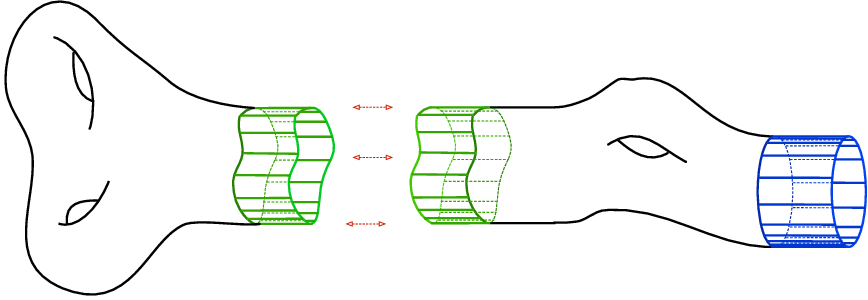
\includegraphics[scale=0.2]{figures/collar.png}
    \caption{Gluing manifolds with collars.}
    \label{fig:collars}
\end{figure}

\begin{defn}[Collar]
    The embedded submanifold $\Phi(\mathcal{O}_p)$ of a manifold $M$ with a boundary constructed above is called a collar of $M$.
\end{defn}

\begin{cor}
    By varying $t$, we find from the above construction that $M$ is homotopy equivalent to $\mathring{M}$.
\end{cor}

Now, if we have two manifolds $M$ and $N$ with diffeomorphic boundaries, so that
\[h:\partial M\to \partial N\text{ -- diffeo},\]
then we can introduce two collar embeddings (which are also diffeo onto their images)
\[
\alpha:[0,1)\times\partial M\to V\subset M,\quad
\beta:[0,1)\times\partial N\to W\subset N,
\]
and unite them by
\[
\Phi: V\sqcup W\to \partial M\times (-1,1),\quad \Phi(x)=
\begin{cases}
(p,-t),& x=\alpha(p,t)\in V,\\
(h(q),t),& x=\beta(q,t)\in W.
\end{cases}
\]
Clearly $\Phi$  is a topological embedding with a closed image (it's surjective), therefore $\Phi$ is a closed mapping.

Now let $\pi:M\sqcup N\to X$ be the quotient map on whose fibers $\Phi$ is constant. Then $\Phi$ descends to $\wt{\Phi}:X\to [-1,1]\times\partial M$. $\Phi$ is continuous and bijective, $\wt{\Phi}(K)=\Phi(\pi^{-1}(K))$ is closed for any compact $K$ (because $\Phi$ is closed and $\pi$ is continuous), so $\wt{\Phi}$ is closed too. Therefore $\wt{\Phi}$ is a homeomorphism and therefore a diffeomorphism, and $X$ is a quotient manifold. Alternatively, this follows from the \emph{closed graph theorem}, which states that the graph of any continuous mapping into a Hausdorff space is closed.

\begin{defn}[Gluing of manifolds]
    The construction described above is called the gluing of two manifolds with diffeomorphic boundaries, denoted by $M\cup_h N$. See Figure~\ref{fig:collars}.
\end{defn}

\begin{defn}[Connected sum]\index{Connected sum of manifolds}
    Let $M_i$, $i=1,2$ be two connected manifolds without boundaries and $M_i'=M_i\setminus U_i$, where $U_i$ is a coordinate ball. We can pick two diffeomorphisms $h_i:\partial M_i'\to \bbS^{n-1}$, $i=1,2$. Then we define the connected sum as the gluing along $h_1\circ h_2^{-1}$:
    \[M_1 \# M_2\coloneqq M_1'\cup_{h_1\circ h_2^{-1}}M_2'.\]
\end{defn}
\begin{example}
    $D(M)=M\cup_{\partial M}M$ is called the \emph{double} of a manifold with a boundary.
\end{example}
\begin{example}
    f $X\parallel \partial D$, $D\subset M$, then $F^X$ leaves $D$ invariant.
\end{example}
\begin{cor}
    If $X\parallel \partial M$, then the theorem about the existence of flows applies to $X$.
\end{cor}
\begin{proof}
    Extend $X$ to the double $D(M)$, apply the flow theorem there, then restrict to $M$.
\end{proof}
\begin{example}
So far we've only considered time-independent vector fields. In general, we can have a time-dependent vector field $X:M\times J\to TM$, $J\subset\bbR $. All of the results about flows still hold almost unchanged, only now the flow map (``evolution operator'') depends on two time parameters: $F^X(p,t_1,t_2)$.
\end{example}

\begin{thm}[Rectification/Straightening Theorem]\index{Theorem!Rectification/Straightening}\label{rectification}
If $X\in\fX(M)$ and $X(p)\neq 0$, then there exists a local chart $(U,\varphi)$ at $p$ such that its slice $S=\{p\in U\mid \varphi^1(p)=0\}$ is diffeomorphic to $\bbD^{n-1}$, $X(p)\notin T_p S$ and $X=\partial_1$ on $U$.
\end{thm}
\begin{proof}
Since $S\sub M$, it has a slice neighborhood. We can parametrize $S$ by an embedding map $x:\Omega\to S$ with $\Omega\mathring{\subset}\bbR^{n-1}$. We can take $U$ such that $\restr{X}{U}\cap TS=\varnothing$. 

Now we can use a flow-out along $X$ so that the flow $F_t(x(s))$ parametrizes $F(x(\Omega))\sub M$. This is a diffeo $\mathcal{O}_\delta\to F(x(\Omega))=x(\Omega)_\delta$ and hence has a smooth inverse. The inverse then gives a local chart $\varphi=\psi^{-1}$, where $\psi(s,t)=F_t(x(s))$. Finally, $X=\partial_t=\partial_1$ in this local chart.
\end{proof}

\begin{defn}[Complete integral]\index{Complete integral}\label{def complete integral}
    A complete integral of a vector field $X\in \fX(M)$, $\dim M=n$, is a local function $\Psi:U\times I_\epsilon\to\bbR^n$ such that $\Psi^{-1}(\bf{c})$ for every $\bf{c}\in\bbR^n$ in the image of $\Psi$ is an integral curve of $X$ at a point $m\in U$. The components $\Psi^i:U\times I_\epsilon\to \bbR$ of this map are called a \emph{complete set of integrals of motion} for $X$.
\end{defn}
\begin{prop}
    Local complete integrals exists for all vector fields.
\end{prop}
\begin{proof}
    First rectify the vector field, then the coordinates $\bf{c}=(\varphi^1(s),\varphi^2(s),\ldots,\varphi^n(s))$ of the point $s$ of intersection of each integral curve with the slice $S$ will be the (constant) value of the diffeomorphism $\Psi:(s,t)\mapsto \varphi(F_t(s))$ on this whole curve.
\end{proof}




\subsection{Vector fields as differential operators}

Recall that Lie derivatives of functions satisfy $\Lie_{F_\ast X}F_\ast f=F_\ast(\Lie_X f)$ for diffeomorphisms $F$. Also, Lie derivatives are local: for any open set $U$
\[\Lie_{\restr{X}{U}}\left(\restr{f}{U}\right)=\restr{\left(\Lie_X f\right)}{U}.\]

\begin{defn}[Derivations]\index{Derivation on an algebra}
If $A$ is an algebra over a field $\bbK$, then a derivation on $A$ is a $K$-linear map $D:A\to A$ that satisfies the Leibniz rule
\[D(a\cdot b)=D(a)\cdot b+a\cdot D(b),\;\; a,b\in A.\]
Is is easy to check that the vector space of all derivations on $A$, denoted by $\mathrm{Der}(A)$, is a Lie algebra under the commutator $[D_1,D_2]=D_1\circ D_2-D_2\circ D_1$.
An algebra with a distinguished derivation is called a \emph{differential algebra}.
\end{defn}

Clearly any Lie derivative $\Lie_X, X\in\fX(M)$, is a derivation on the algebra of functions $C^\infty(M)$, because it is a directional derivative in local coordinates.
Moreover, any derivation $D$ on $C^\infty(M)$ satisfies $D(1)=0$, because
\[D(1)=D(1^2)=D(1)\cdot 1+1\cdot D(1)=2\cdot D(1).\]
Finally, the set of all Lie derivatives $\{\Lie_X\}_{X\in\fX(M)}$ is a $C^\infty(M)$-module:
\[f\cdot\Lie_X=\Lie_{f\cdot X}.\]

\begin{prop}[{{\cite[Prop.~2.2.9]{Marsden}}}]\label{prop 2.2.9 Marsden}
    The vector space of Lie derivatives $\{\Lie_X\}_{X\in\fX(M)}$ is isomorphic to $\fX(M)$ as $C^\infty(M)$-modules. In particular, $\Lie_X=0$ iff $X=0$.
\end{prop}
\begin{proof}
    The map $X\mapsto \calL_X$ is clearly $C^\infty(M)$-linear and surjective by definition. To show that it is an isomorphism, we need to show that its kernel is zero. Suppose $\calL_X=0$ and $m\in M$. Then $\dd_m f(X_m)=0$ for all $f\in C^\infty(M)$, and hence $\alpha_m(X_m)=0$ for all $\alpha_m\in T_m^\ast M$. But then $X_m=0$.
\end{proof}
\begin{prop}[{{\cite[Thm.~2.2.10]{Marsden}}}]\label{lie derivatives and vector fields}
The space of all $\bbR $-linear derivations on the algebra $C^\infty(M)$ is isomorphic to $\fX(M)$ as a vector space. In particular, every derivation $\theta$ coincides with $\Lie_X$ for a unique $X\in\fX(M)$.
\end{prop}
\begin{proof}
    Given $\theta$, we construct the vector field $X$.
    First of all, $\theta$ is local, i.e.\ if $h$ vanishes on a neighborhood $V\mathring{\subset} M$ of $p\in V$, then $\theta(h)(p)=0$. Indeed, if $\chi$ is a bump function equal to $1$ around $p$ and zero outside of $V$, then $h=(1-\chi)h$ and
    \[\theta(h)(p)=(\theta(1-\chi))\cdot h(p)+\theta(h)\cdot (1-\chi(p))=0.\]

    Pick a local chart at $p$, $\varphi:U\to\wh{U}\subset\bbR^n$. Let $\bf{x}\in\wh{U}$, $\bf{a}=\varphi(p)$, $f\in C^\infty(M)$, then 
    \[(\varphi_\ast f)(\bf{x})=(\varphi_\ast f)(\bf{a})+\sum_{j=1}^n (x^j-a^j)\int_0^1 \frac{\partial(\varphi_\ast f)}{\partial x^j} (\bf{a}+t(\bf{x}-\bf{a}))\dd t\]
    on some neighborhood of $\bf{a}$.
    Therefore, for $u\in U$,
    \[f(u)=f(p)+\sum_{i=1}^n (\varphi^i(u)-a^i)g_i(u),\quad g_i(p)=\frac{\partial(\varphi_\ast f)}{\partial x^i} (\varphi(p)).\] 
    Thus,
    \[(\theta f)(p)=\sum_i g_i(p)\theta(\varphi^i)(p)=\sum \partial_{x^i}(\varphi_\ast f)(\bf{a}) \theta \varphi^i(p),\]
    and this is formula is chart-independent! Now we can define a smooth $X$ by its local representation
    \[X^i(u)\coloneqq \theta\varphi^i(u).\]
    It is easy to check that $X$ is independent of the choice of $\varphi$, which means that it is actually a globally well-defined vector field on $M$. For $f\in C^\infty(M)$, the local representative in $\bf{x}=\varphi(u)\in\wh{U}$ of $\Lie_X f$ is 
    \[(f\circ\varphi^{-1})_{\ast \bf{x}}\circ \wh{X}(\bf{x})=\sum_i \partial_{x^i}(f\circ \varphi^{-1})(x)\cdot \theta \varphi^i (u)=\theta f(u),\]
    hence $\theta=\Lie_X$.
    Uniqueness follows from the obvious statement that $\Lie_X=0$ iff $X=0$.
\end{proof}
\begin{cor}
If $x^i$ is a local coordinate system, then the local vector fields $\partial_i=\partial_{x^i}$ form a basis of derivations at $p$, therefore 
\[(\Lie_X f)(p)=\sum_i \partial_{x^i}(f\circ\varphi^{-1})(\varphi(p))\cdot \underbrace{\Lie_X (\varphi^i)(p)}_{X^i}=\sum_i X^i \partial_{x^i}(\varphi_\ast f)=\sum_i X^i \partial_{i} f.\]
\end{cor}

\begin{prop}
If $X,Y\in\fX(M)$, then $[\Lie_X,\Lie_Y]=\Lie_X\Lie_Y-\Lie_Y\Lie_X$ is a derivation on $C^\infty(M)$.
\end{prop}
\begin{proof}
    This is a very general property that the commutator of two derivations is always a derivation:
    \begin{multline}
        [D_1,D_2](fg)=D_1((D_2f)g+f(D_2g))-D_2((D_1f)g+f(D_1g))=\\=([D_1,D_2]f)g+f([D_1,D_2]g).
    \end{multline}
\end{proof}

This proposition allows us to define the commutator of vector fields.

\begin{defn}[Lie derivative/bracket of vector fields]\index{Lie derivative of vector fields}\index{Commutator of vector fields}
If $X,Y\in\fX(M)$, then the Lie derivative of $Y$ along $X$ is denoted by 
\[\Lie_X Y\equiv [X,Y]\] and is defined as the unique vector field such that
\[\Lie_{[X,Y]}=[\Lie_X,\Lie_Y].\]
With this bracket, $\fX(M)$ becomes a Lie algebra that is isomorphic to the Lie algebra of derivations on $C^\infty(M)$ (i.e.\ Lie derivatives).
In local coordinates (using Einstein summation),
\[[X,Y]^j=X^i \partial_i Y^j-Y^i \partial_i X^j.\label{eq Lie derivative in components}\]
\end{defn}

\begin{prop}\label{prop properties of Lie derivatives}
\begin{enumerate}
    \item $[X,Y]$ is local and natural w.r.t.\ diffeomorphisms, i.e.\ \[F_\ast [X,Y]=[F_\ast X,F_\ast Y];\]
    \item $\Lie_X$ is a derivation on the Lie algebra $\fX(M)$, i.e.\ satisfies the Jacobi identity
    \[\Lie_X [Y,Z]=[\Lie_X Y,Z]+[Y,\Lie_X Z];\]
    \item $\Lie_X$ is also a derivation on $C^\infty(M)\otimes \fX(M)$ i.e.\ it satisfies the mixed Leibniz rule
    \[\Lie_X(f\otimes Y)=\Lie_X(f\cdot Y)=(\Lie_X f)\cdot Y+f\cdot \Lie_X Y.\]
    Equivalently, 
    \[\Lie_{fX}Y=f\cdot \Lie_X Y+\left(\Lie_X f\right)\cdot Y.\label{Lie derivative not covariant}\]
\end{enumerate}
\end{prop}
\begin{proof}
    \begin{enumerate}
        \item To prove any of these properties, we act with both sides on a function $f$ as a Lie derivative. Then the equality of the two expressions as derivations implies the equality as vector fields by Proposition \ref{lie derivatives and vector fields}. Therefore this is just a direct computation using the push-forward property for Lie derivatives acting on functions.
        \item General property of derivations that is easily checked by expanding both sides.
        \item Check 
        \begin{multline}
            [X,fY]g=\Lie_X (\Lie_{fY}g)-\Lie_{fY}\Lie_X g=\Lie_X (f\Lie_Y g)-f\Lie_Y \Lie_X g=\\=(\Lie_X f)\Lie_Y g+f\Lie_X\Lie_Y g-f\Lie_Y\Lie_X g=((\Lie_X f)Y+f[X,Y])g.
        \end{multline}
    \end{enumerate}
\end{proof}


\begin{rem}[Lie derivatives are not covariant derivatives]\label{rem: Lie derivatives not covariant}
    Property (\ref{Lie derivative not covariant}) shows that $L_X Y$ doesn't behave like a tensor with respect to $X$ (or $Y$), since it is not $C^\infty(M)$-linear in it. This is why Lie derivatives are not a special case of \emph{covariant} derivatives.
    
    A covariant derivative (of vector fields) is a map $\nabla:\fX(M)\otimes\fX(M)\to \fX(M)$ denoted by $X,Y\mapsto \nabla_X Y$ such that it satisfies:
    \begin{itemize}
        \item $C^\infty(M)$-linearity in $X$: $\nabla_{fX}Y=f\cdot \nabla_X Y$ for $f\in C^\infty(M)$;
        \item $\bbR $-linearity in $Y$: $\nabla_X (\alpha Y+Z)=\alpha \nabla_XY+\nabla_XZ$ for $\alpha\in\bbR $;
        \item Leibniz rule: $\nabla_X(f\cdot Y)=(\Lie_X f)\cdot Y+f\cdot \nabla_X Y.$
    \end{itemize}
    Therefore any covariant derivative $\nabla_X Y$ has to be a tensor in $X$, unlike Lie derivatives. In other words, a covariant derivative can be thought of as a map $\nabla:\fX(M)\to \fX^\ast(M)\otimes\fX(M)=\Gamma^1_1(M)$, $Y\mapsto \nabla Y\in\Gamma^1_1(M)$.
\end{rem}

All of this allows us to extend the Lie derivative to tensor fields of any rank by the following theorem.

\begin{defn}[Tensor differential operators]\index{Differential operator on the tensor algebra}
A differential operator on the tensor algebra $\Gamma^\infty(M)$ is a collection of maps $\mathbb{D}^r_s(U):\Gamma^r_s(U)\to \Gamma^r_s(U)$ for all $r,s\geq 0$ and each open $U\mathring{\subset}M$ (we denote them all by $\mathbb{D}$) such that:
\begin{enumerate}
    \item $\mathbb{D}$ is a tensor derivation (w.r.t.\ $\otimes$);
    \item $\mathbb{D}$ is local, i.e.\ for $U\subset V$ and $t\in\Gamma^r_s(V)$, $\restr{\mathbb{D}(t)}{U}=\mathbb{D}(\restr{t}{U})$;
    \item $\mathbb{D} \delta=0$, where $\delta\in\Gamma^1_1(M)$ is the Kronecker tensor $\delta=\id_{TM}$.
\end{enumerate}
\end{defn}

Note that we don't require $\mathbb{D}\circ\varphi_\ast=\varphi_\ast\circ \mathbb{D}$ because this will not hold for covariant derivatives, which we would still like to consider differential operators.

\begin{thm}[Willmore {{\cite[Thm.~2.2.17]{Marsden}}}]\index{Theorem!Willmore}\label{Willmore}
A collection of local tensor derivations $E_U$ on $C^\infty(U)$ and $F_U$ on $\fX(U)$ (which agree with each other via the mixed rank Leibniz rule) for each $U\mathring{\subset}M$ determines a unique differential operator $\mathbb{D}$ on the tensor algebra $\Gamma^\infty(M)$ that coincides with $E_U$ on $C^\infty$ and with $F_U$ on $\fX$.
\end{thm}
\begin{proof}
    Suppose we know that such a $\mathbb{D}$ exists. In a local frame $\{e_i\}$ and dual frame $\{\alpha^i\}$, we can write
    \[t(u)=\underbrace{t_{j_1\ldots j_s}^{i_1\ldots i_r}(u)}_{\in C^\infty(U)} e_{i_1}\otimes \cdots \otimes e_{i_r}\otimes \alpha^{j_1}\otimes \cdots\otimes \alpha^{j_s}(u).\label{535}\]
    By using the tensorial Leibniz rule for $\mathbb{D}$, we express $\mathbb{D}t(u)$ only in terms of $E_U(t_{j_1\ldots j_s}^{i_1\ldots i_r})$ and $F_U(e_{i_k})$.
    
    Namely, since $\mathbb{D}\delta=0$, and $\delta=e_j\otimes \alpha^j$ (using Einstein summation), we have 
    \[0=\mathbb{D}(e_j\otimes \alpha^j)=(\mathbb{D}e_j)\otimes \alpha^j+e_j\otimes (\mathbb{D}\alpha^j).\]
    Since $\delta^i_j=\alpha^i(e_j)$, if we contract the formula above with $e_i$, we get
    \[0=F_U e_i+(\mathbb{D}\alpha^j)(e_i) e_j,\]
    which completely determines $\mathbb{D}\alpha^j$. Therefore the action of $\mathbb{D}$ on $\fX^\ast$ is uniquely determined, and the Leibniz rule applied to \ref{535} gives a formula for $\mathbb{D}$ in terms of $E_U$ and $F_U$ on the whole tensor algebra.
    
    The formulas we have derived prove the uniqueness of $\mathbb{D}$. Its existence follows from the fact that these same formulas define a valid differential operator that satisfies all the requirements of the theorem.
\end{proof}
\begin{cor}\label{cor willmore formula}
A byproduct of the theorem above is the general formula for differential operators on the tensor algebra:

\begin{multline}
    \mathbb{D}\left(t(\alpha^1,\ldots,\alpha^r,X_1,\ldots,X_s)\right)=(\mathbb{D}t)(\alpha^1,\ldots,\alpha^r,X_1,\ldots,X_s)+\\+\sum_{j=1}^r t\left(\alpha^1,\ldots,\mathbb{D}\alpha^j,\ldots,\alpha^r,X_1,\ldots,X_s\right)+\sum_{k=1}^s t\left(\alpha^1,\ldots,\alpha^r,X_1,\ldots,\mathbb{D}X_k,\ldots,X_s\right).
\end{multline}
This formula essentially states that $\mathbb{D}$ ``commutes with contractions''.
\end{cor}

\begin{defn}[Lie derivatives of tensors]\index{Lie derivative of tensor fields}
If $X\in\fX(M)$ then the Lie derivative operator $\Lie_X$ on the tensor algebra $\Gamma^\infty(M)$ is defined as the unique tensor differential operator (established by Willmore's theorem) that coincides with the previously constructed Lie derivative on $C^\infty(M)$ and $\fX(M)$.
\end{defn}

\begin{prop}[Naturality of Lie derivatives]\label{pullbacks of Lie derivatives}
For a diffeomorphism $F$, 
\[\Lie_{F_\ast X}(F_\ast t)=F_\ast (\Lie_X t).\]
\end{prop}
\begin{proof}
Define an operator $\mathbb{D}$ by $\mathbb{D}t=F^\ast \Lie_{F_\ast t}(F_\ast t)$. We know that $\mathbb{D}$ coincides with $\Lie_X$ on $C^\infty$ and $\fX(M)$. It is also easy to check that $\mathbb{D}$ is a tensor differential operator (Exercise). Then, by Willmore's Theorem, is must coincide with $\Lie_X$ on the entire tensor algebra.
\end{proof}


\begin{comment}
    \begin{samepage}
        \PRLsep
        \begin{center}
            {\red Lecture 14 on 1 Mar 2019 ended here}
        \end{center}
    \end{samepage}
\end{comment}


\subsection{Geometric approach to Lie derivatives}

Let $X\in \fX(M)$ and let $(U,a,F)$ be a flow box of $X$ at $p\in M$. Let $t\in\Gamma^r_s(M)$ and define
\[t_\lambda\coloneqq F_{\lambda}^\ast \left(\restr{t}{U_\lambda}\right)=F_{\lambda\ast}^{-1} \left(\restr{t}{U_\lambda}\right)\in\Gamma^r_s(U),\]
where $F_\lambda :U\to U_\lambda$ is the flow diffeomorphism. Then with fixed $p$, the map $\lambda\mapsto t_\lambda (p) \in \bbT^r_s (T_p M)$ defines a curve in the vector space of tensors at $p$.
\begin{thm}
    $\lambda\mapsto t_\lambda (p)$ defined above is a curve in the vector space $\bbT^r_s (T_p M)$ passing through $t(p)$ and its derivative evaluates the Lie derivative of $t$:
    \[\Lie_X t(p)=\restr{\frac{\dd}{\dd \lambda}}{\lambda=0}t_\lambda(p).\]
\end{thm}
\begin{proof}
    We have 
    \[t_\lambda(p)=(\bbT^r_s F_\lambda^{-1})\circ t \circ F_\lambda(p),\] 
    which is clearly smooth.
    Define $\theta_X$ as an operator on $\Gamma^r_s(M)$ by 
    \[\theta_X t(p)=\restr{\frac{\dd}{\dd \lambda}}{\lambda=0} t_\lambda(p).\]
    For $t\in C^\infty(M)$, $t_\lambda(p)$ is smooth, therefore $\theta_X t(p)=(Tt_\bullet)(\partial_\lambda)\in C^\infty(M)$, where the differential $T$ is with respect to the variable $\lambda$ (represented by $\bullet$) and  $\partial_\lambda$ is a vector field on the $\bbR $. $\theta_X$ is a linear derivation because its local representatives are. It is defined locally, therefore it is local. Finally, 
    \[\theta_X\delta=\restr{\frac{\dd}{\dd \lambda}}{\lambda=0} F^\ast_\lambda \delta=\restr{\frac{\dd}{\dd \lambda}}{\lambda=0}\delta=0.\] 
    This proves that $\theta_X$ is a differential operator. It remains to check that $\theta_X=\Lie_X$ on $C^\infty(M)$ and $\fX(M)$. First, for $f\in C^\infty(M)$, 
    $f_\lambda=f\circ F_\lambda$, 
    \[\restr{\frac{\dd}{\dd \lambda}}{\lambda=0}f_\lambda(p)=\dd f\circ \restr{\frac{\dd}{\dd \lambda}}{\lambda=0}F_\lambda=\dd f\circ X=\Lie_X f.\]
    Now, note that for $f\in C^\infty(M)$ there exists a $g_\lambda\in C^\infty(M)$ such that $g_0=\Lie_X f$ and $f\circ F_\lambda=f+\lambda g_\lambda$. Namely, 
    \[\lambda g_\lambda (p)=\int_0^1 \partial_t(f\circ F_{t\lambda}(p))\dd t.\] 
    Then for $Y\in\fX(M)$,
    \begin{align}
        \Lie_{\theta_X Y}f(p)=&\dd f\circ \restr{\frac{\dd}{\dd \lambda}}{\lambda=0} \left((F_{-\lambda})_{\ast p}\circ Y\circ F_\lambda(p)\right)=\\
        =&\restr{\frac{\dd}{\dd \lambda}}{\lambda=0}\left((f\circ F_{-\lambda})_\ast\circ Y\circ F_\lambda(p)\right)=\\
        =&\restr{\frac{\dd}{\dd \lambda}}{\lambda=0} \left((f-\lambda g_{-\lambda})_\ast\circ Y\circ F_\lambda(p)\right)=\\
        =&\restr{\frac{\dd}{\dd \lambda}}{\lambda=0} f_\ast\circ Y\circ F_\lambda (p)-\restr{\left(\frac{\dd}{\dd \lambda}\lambda\right)(g_{-\lambda})_\ast\circ Y\circ F_\lambda(p)}{\lambda=0}=\\
        =&\dd(\underbrace{f_\ast\circ Y}_{\Lie_Yf})\circ \underbrace{\restr{\frac{\dd}{\dd \lambda}}{\lambda=0} F_\lambda(p)}_{X(p)}-(g_0)_\ast \circ Y\circ F_0(p)=\\
        =&\Lie_X\Lie_Y f-\Lie_Y\Lie_X f(p),
    \end{align}
    therefore $\theta_X Y=[X,Y]$. By Willmore's theorem, $\theta_X=\Lie_X$.
\end{proof}
\begin{cor}
\begin{enumerate}
    \item $\Lie_X t=0$ iff $t$ is constant along the flow of $X$: $F^\ast_\lambda t=t$;
    \item For all $\lambda$ in the flow domain the following equality holds:
    \[\frac{\dd}{\dd \lambda}F^\ast_\lambda t=F^\ast_\lambda \Lie_X t.\]
    In particular, 
    \[\Lie_X t=F^\ast_{-\lambda} \frac{\dd}{\dd \lambda}F^\ast_\lambda t=\restr{\frac{\dd}{\dd\lambda}}{\lambda=0}F^\ast_\lambda t.\]
\end{enumerate}
\end{cor}

\begin{rem}[Push-forwards are not parallel transports]
    Since covariant derivatives are in the exact same relationship with parallel transports as Lie derivatives are with push-forwards, it is tempting to think that Lie derivatives are special cases of covariant derivatives. However, we have already seen this to be wrong in Remark \ref{rem: Lie derivatives not covariant}. This means that push-forwards by flows of vector fields cannot be interpreted as a kind of parallel transport along the integral curves of those vector fields. This is because a parallel transport has to be unambiguously defined for every curve on $M$, whereas there are infinitely many vector fields for which a given curve is integral (and the value of the push-forward will depend on the specific choice of vector field). Transport by push-forwards is often called \emph{Lie transport}\index{Lie transport}. Lie derivatives are just infinitesimal Lie transport.
\end{rem}

\begin{rem}
    We can apply these ideas to PDEs on $\bbR^n$:
    \[\begin{cases}
        \partial_t f(x,t)=\sum _i X^i \partial_i f(x,t),&\\
        f(x,0)=g(x).&
    \end{cases}\]
    Then if $X$ has a complete flow $F_t$, the unique solution of the above Cauchy problem is $f(x,t)=g(F_t(x))$, which can be checked by substitution. This is sometimes called the \emph{method of characteristics}. The ``characteristics'' are the integral curves along which the values of $g(x)$ get propagated.
\end{rem}

\begin{prop}
    Given two vector fields $X,Y$ with complete flows $F_t$ and $G_t$, respectively, \gls{tfae}:
    \begin{enumerate}
        \item $[X,Y]=0$;
        \item $F^\ast_t Y=Y$ (or $G^\ast_t X=X$);
        \item $F_t\circ G_s=G_s\circ F_t$ for all $t,s$. 
    \end{enumerate}
    In particular, the flow of $X+Y$ for commuting $X$ and $Y$ is $F_t\circ G_t$.
\end{prop}
\begin{proof}
    $1\Rightarrow 2$. $\frac{\dd}{\dd t}F^\ast_t Y=F^\ast_t \Lie_X Y=0$, therefore $F^\ast_t Y$ is constant and we know that $F^\ast_0 Y=Y$, so $F^\ast_t Y=Y$.

    $2\Rightarrow 3$. Consider the curve $\gamma(t)=G_s\circ F_t(p)$. It starts at $\gamma(0)=G_s(p)$ and its velocity is
    \[\dot\gamma(t)=\frac{\dd}{\dd t} G_s\circ F_t(p)=G_{s\ast}\circ X\circ F_t\overset{(2)}{=}X\circ\gamma(t).\]
    So $\gamma(t)$ is an integral curve of $X$ going through $p$. Therefore, by uniqueness (and definition of the flow of $X$), 
    \[\gamma(t)=F_t\circ G_s(p).\]
    This shows that the flows commute. Finally, we check 
    \[\frac{\dd}{\dd t} F_t\circ G_t(p)=X(F_t(G_t(p)))+\underbrace{F_{t\ast }Y}_{Y\circ F_t}(G_t(p))=(X+Y)(F_t\circ G_t(p)).\]

    $2\Rightarrow 1$. $\Lie_X Y=F^\ast_{-t}\frac{\dd}{\dd t}F^\ast_t Y=F^\ast_{-t} \frac{\dd}{\dd t}Y=0$.

    $3\Rightarrow 2$. $F_{t\ast}Y=F_{t\ast}\frac{\dd}{\dd s}G_s=F_{t\ast} G_{s\ast} Y=(F_t\circ G_s)_\ast Y=(G_s\circ F_t)_\ast Y=G_{s\ast}F_{t\ast}Y$. But the only vector field invariant under $G_{s\ast}$ is $Y$, therefore $F_{t\ast}Y=Y$.
\end{proof}

\begin{rem}[Taylor formula on manifolds]\index{Taylor's formula}\label{rem 3.2.9 RS1}
    Successive application of the vector fields $X_1,\ldots,X_r$ to a function $f\in C^\infty(M)$ yields
    \[X_r\cdots X_1 \cdot f=\restr{\frac{\dd}{\dd t_1}}{t_1=0}\cdots \restr{\frac{\dd}{\dd t_r}}{t_r=0}f\circ F^{X_1}_{t_1}\circ \cdots \circ F^{X_r}_{t_r}.\]
    In particular, the Lie bracket can be expressed as
    \[[X,Y]f=\restr{\frac{\dd}{\dd t}}{t=0}\restr{\frac{\dd}{\dd s}}{s=0}\left(f\circ F^Y_s\circ F^X_t-f\circ F^X_s\circ F^Y_t\right).\label{eq Lie bracket in terms of flows}\]
    Furthermore, for any $m\in M$, the Taylor expansion of the smooth function $t\mapsto f\circ F^X_t(m)$ at $t=0$ yields the following \emph{Taylor formula for manifolds}:
    \[f\circ F^X_t(m)=\sum_{k=1}^n\frac{t^k}{k!}\left(X^kf\right)(m)+\calO(t^{n+1}), \quad t\in \calD^X_m,\label{eq:Taylor formula for manifolds}\]
    where $\calO(t^{n+1})$ is a smooth function on $\calD_m^X$ such that $\calO(t^{n+1})/t^{n+1}$ is bounded. By defining the exponential of a differential operator formally as $\rme^{tD}=\sum_{k=0}^\infty \frac{t^k}{k!}D^k$, the above Taylor formula is sometimes written formally as $f\circ F^X_t=\rme^{t X}\cdot f$.

    Repeated application of this formula yields the iterated Taylor formula for manifolds
    \[f\circ F^X_t\circ F^Y_s(m)=\sum_{k,l=1}^n\frac{t^ks^l}{k!l!}\left(Y^lX^kf\right)(m)+\calO(t^{n+1},s^{n+1}),\label{eq: Taylor formula for two fields}\]
    which easily generalizes to any number of vector fields.
\end{rem}


\begin{defn}[Holonomic frame]\index{Holonomic frame}
    A local $k$-frame $\{e_i\}_{i=1}^k$ is called holonomic if $[e_i,e_j]=0$ for all $i,j$.
\end{defn}

The following shows that this definition of holonomic frames agrees with the one indicated in Definition~\ref{def jet bundles}. That is, each holonomic frame arises from some local coordinates.

\begin{thm}[Rectification of frames]\index{Theorem!Rectification}\label{thm rectification}
    Let $\{e_j\}_{j=1}^k$ with $k\leq n=\dim M$ be a holonomic local $k$-frame on $W\mathring{\subset}M$. Assume that $e_j(p)\notin T_p S$ for all $p\in S$, where $S\sub M$ is a submanifold with $\codim S=k$. Then there exists a local chart of coordinates $(s^1,\ldots,s^n)$ in which $S=\{s^1=\cdots=s^k=0\}$ and for $j\leq k$ we have $\partial_j=e_j$.
\end{thm}
\begin{proof}
    Parametrize $S$ as usual by $x:\Omega\to S$ with $\Omega\mathring{\subset}\bbR^{n-k}$, define a chart $\varphi=\psi^{-1}$, where
    \[\psi(s^1,\ldots,s^k,s^{k+1},\ldots,s^n)=F^{e_1}_{s_1}\circ\cdots\circ F^{e_k}_{s_k}(x(s^{k+1},\ldots,s^n)),\]
    and $F^{e_i}$ is the flow of $e_i$. The inverse $\psi^{-1}$ exists locally because the differential at $(0,\ldots,0)$ is identity. Finally we use commutation to compute the partials
    \begin{multline}
        \psi_\ast (\partial_{s^i})\cdot f=\partial_i(f\circ\psi)=\partial_i f(F^{e_1}_{s_1}\cdots F^{e_k}_{s_k} x(0,\ldots,0,s^{k+1},\ldots))=\\=\partial_i f(F^{e_i}_{s_i}\circ\cdots )=\partial_i F^{e_i}_{s_i}(F\cdots F(0,\ldots,0,s^{k+1},\ldots))f=e_i\cdot f=\Lie_{e_i}f,
    \end{multline}
    thus $\partial_i=e_i$.
\end{proof}

\begin{cor}
    A helpful way to reformulate this theorem for $k=\dim M$ is: a given local frame is a coordinate frame for some local coordinates if and only if it is holonomic.
\end{cor}

The analog of this Corollary for $k<\dim M$ is a famous theorem that deserves its own section.





\subsection{Frobenius theorem I}\label{sec: frobenius i}

We have just established that in the presence of a local holonomic $r$-frame $\{e_i\}_{i=1}^r$ transversal to a submanifold $S$, each point $m\in S$ admits a $r$-dimensional embedded submanifold $N$ passing through $m$ (defined by holding the values of $s^{r+1},\ldots,s^n$ constant) transversally to $S$ such that $\{e_i\}_{i=1}^r$ is a frame for $TN$. In this section we will replace holonomic frames by the subspaces of tangent spaces that they span and derive the corresponding \emph{integrability condition}. Namely, while we can think of vector fields as fields of velocities, let us unstead think of them as fields of lines, or directions. Then it is easy to generalize the problem as follows: given a field of hyperplanes (subspaces of tangent spaces), what does it mean for a submanifold to be integral for this field, and what is the condition for this kind of integrability?

\begin{hrem*}
    Note that while this theorem is universally named after Frobenius, his result (1887) was an application of an older result to the context of systems of differential equations. We will discuss that version of the theorem in \sect~\ref{sec: frobenius ii}. The results discussed in this \sect{} were obtained by Deahna (sufficient condition, 1840) and Clebsch (necessary condition, 1866), among many others involved in this long process.
\end{hrem*}

\begin{figure}
    \centering
    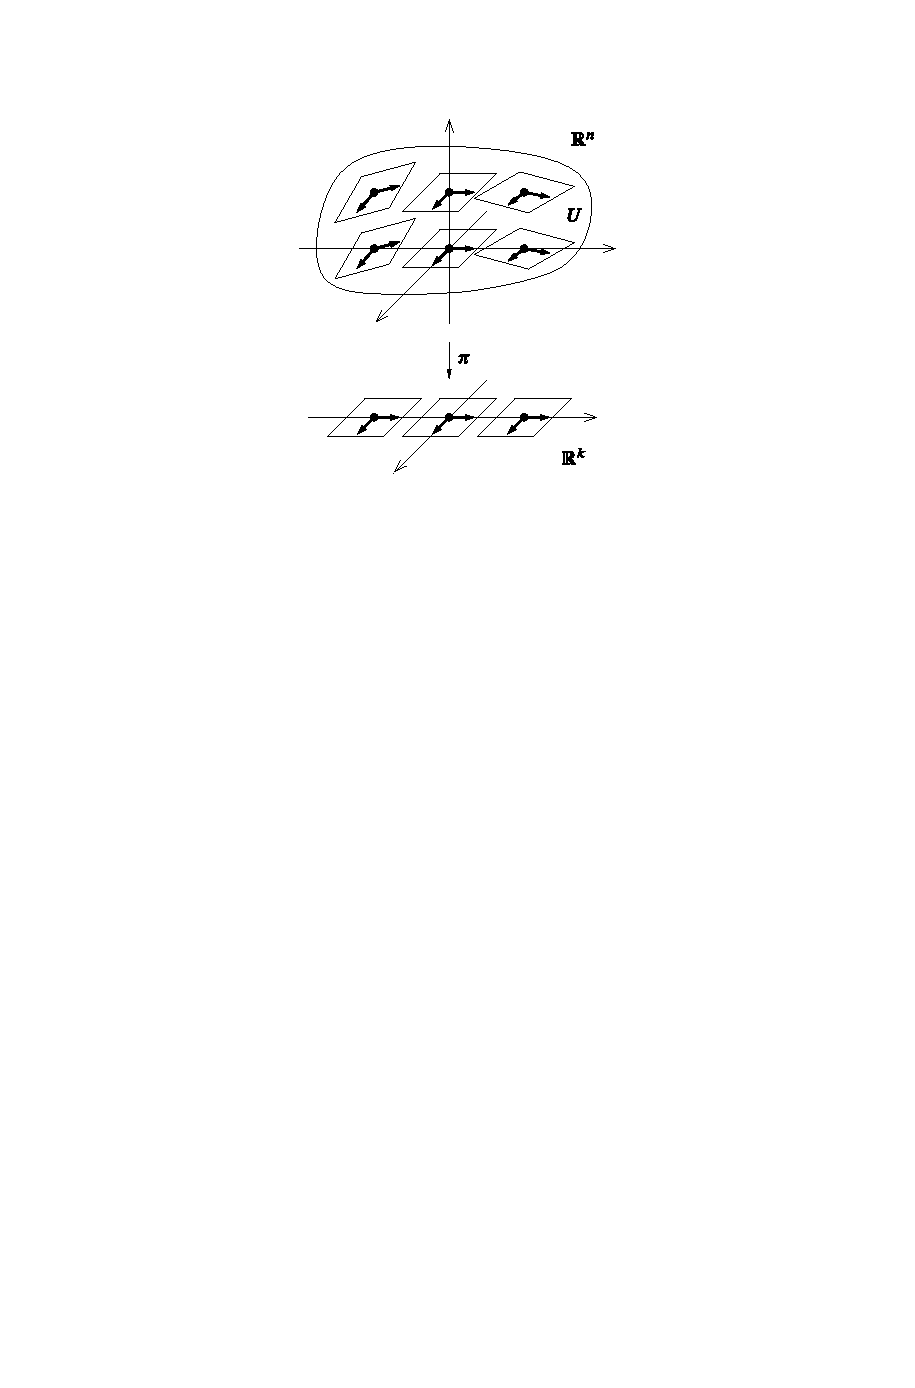
\includegraphics[scale=0.8]{figures/frobenius_1.pdf}
    \caption{Frobenius Theorem. From \cite{Lee}.}
    \label{fig: frobenius1}
\end{figure}

Recall that a distribution $D$ on a manifold is an assignment of a subspace $D_m\subset T_m M$ for every $m\in M$. If the dimension of $D_m$ is constant and equal to $r$, then $D$ is said to be \emph{regular of rank} $r$. $D$ is called a \emph{smooth distribution} if it is a subbundle of $TM$.

\begin{defn}[Integral manifolds]\index{Integral manifold}
    Let $D< TM$ be a smooth distribution (i.e.\ a subbundle of $TM$). An immersed submanifold $N<M$ is called an integral manifold of $D$ if $T_m N=D_m$ for all $m\in N$.
\end{defn}

\begin{defn}[Integrable distribution]\index{Integrable distribution}
    A smooth distribution $D< TM$ is called integrable if every $m\in M$ is contained in a (local) integral manifold of $D$.
\end{defn}

\begin{defn}[Involutive distribution]\index{Involutive distribution}
    For a smooth distribution $D< TM$, denote by $\Gamma^\infty(D)\subset\fX(M)$ the space of $D$-valued vector fields. $D$ is called involutive if $\Gamma^\infty(D)$ is a Lie subalgebra of $\fX(M)$, i.e.\ $[X,Y]\in\Gamma^\infty(D)$ for all $X,Y\in\Gamma^\infty(D)$.
\end{defn}

\begin{thm}[Frobenius Theorem (Clebsch 1866) {{\cite[Thm.~19.12]{Lee}}}]\index{Theorem!Frobenius}\label{thm frobenius}
    A smooth distribution $D$ is involutive iff it is integrable.
\end{thm}
\begin{proof}
    The backwards direction is trivial: if $D$ is integrable, then $D=TN$ locally, which implies involutivity.
    For the forward direction, it suffices to prove that $D$ is locally spanned by a set of linearly independent commuting fields. Then, by the Rectification Theorem~\ref{thm rectification}, they are coordinate vector fields for a slice chart of an integral manifold.

    Because of the locality of the statement, it also suffices to prove the theorem for $M=U\subset \bbR^n$. Suppose that the rank of $D$ is $r$. Then, at every $m\in M$, we can find a system of Cartesian coordinates such that $D_m$ is complementary to $\Span\{\partial_{r+1},\ldots,\partial_m\}$. By continuity, this remains true on some neighborhood of $m$. Therefore, we have a non-singular projection $\pi:\bbR^m\to\bbR^r$ onto the coordinate hyperplane of the coordinates $(x^1,\ldots,x^r)$. Then $\restr{\pi_\ast}{D}$ is a smooth bundle isomorphism, and the vector fields $\pi^\ast(\partial_i)$, $i=1,\ldots,r$, locally span $D$, see Figure~\ref{fig: frobenius1}. By naturality of Lie derivatives, $[\pi^\ast(\partial_i),\pi^\ast(\partial_j)]=\pi^\ast[\partial_i,\partial_j]=0.$
    Thus, $D$ is indeed spanned by a holonomic $r$-frame and therefore integrable.
\end{proof}

This theorem is of crucial importance in the theory of Lie groups, fiber bundles, and even dynamical systems. The entire concept of \emph{integrability} ultimately stems from it. The rest of this \subsect is devoted to characterizing integral submanifolds and proving a global version of the Frobenius theorem, which will be useful is some applications.

\begin{cor}[{{\cite[Cor.~19.13]{Lee}}}]\label{cor 19.13 Lee}
    Let $D$ be a rank $r$ involutive distribution on $M$. If $S\sub M$ is a codimension $r$ embedded submanifold such that $T_mS\cap D_m=\{0\}$ for all $m\in S$, then there is a \emph{flat chart}\index{Flat chart} $(U,\{s^i\})$ for $S$ centered at $m$ in which $S\cap U$ is the slice $s^1=\cdots=s^r=0$.
\end{cor}
\begin{proof}
    The proof of Frobenius theorem showed that locally $D$ is spanned by $r$ commuting vector fields, so this Corollary follows by the Rectification Theorem~\ref{thm rectification}.
\end{proof}

Note also that $U$ gets decomposed into a disjoint union of integral submanifolds $U_{\bf{c}}$ parametrized by a point $\bf{c}\in S$ with coordinates $(0,\ldots,0,c^1,\ldots,c^{n-r})$ in the flat chart and defined as the slices $s^{r+1}=c^1,\ldots, s^n=c^{n-r}$.

\begin{prop}[{{\cite[Prop~19.16]{Lee}}}]\label{prop 19.16 Lee}
    Let $D$ be an involutive distribution of rank $r$ on a smooth manifold $M$, and let $(U,\{x^i\})$ be a flat chart for $D$. If $N$ is an integral manifold of $D$, then $N\cap U$ is a union of countably many disjoint open subsets of parallel $r$-dimensional slices of $U$, each of which is open in $N$ and embedded in $M$.
\end{prop}
\begin{proof}
    Since the inclusion $i:N\hookrightarrow M$ is continuous, $N\cap U=i^{-1}(U)$ is open in $H$ and this is a coutnable disjoint union of connected components, each open in $N$.

    Let $V$ be a component of $N\cap U$. Since the chart is flat, the functions $x^{r+1},\ldots,x^n$ are constant along $D$ and therefore constant on any connected slice like $V$, and $V$ lies in a single slice $U_{\bf{c}}$, see Figure~\ref{fig: frobenius2}.

    Since $U_{\bf{c}}$ is embedded in $M$, the inclusion $V\hookrightarrow M$ ialso restricts to a smooth map into $U_{\bf{c}}$. The inclusion $V\hookrightarrow U_{\bf{c}}$ is thus an injective smooth immersion between manifolds of the same dimension, and therefore a local diffeomorphism, an open map, and a homeomorphism onto an open subset of $U_{\bf{c}}$. The inclusion map $V\hookrightarrow M$ is a composition of the smooth embeddings $V\hookrightarrow S\hookrightarrow M$ and thus a smooth embedding.
\end{proof}

Recall now that a weakly embedded submanifold $N<M$ is such that any smooth map into $M$ whose values lie in $N$ restricts to a smooth map into $N$.

\begin{figure}
    \centering
    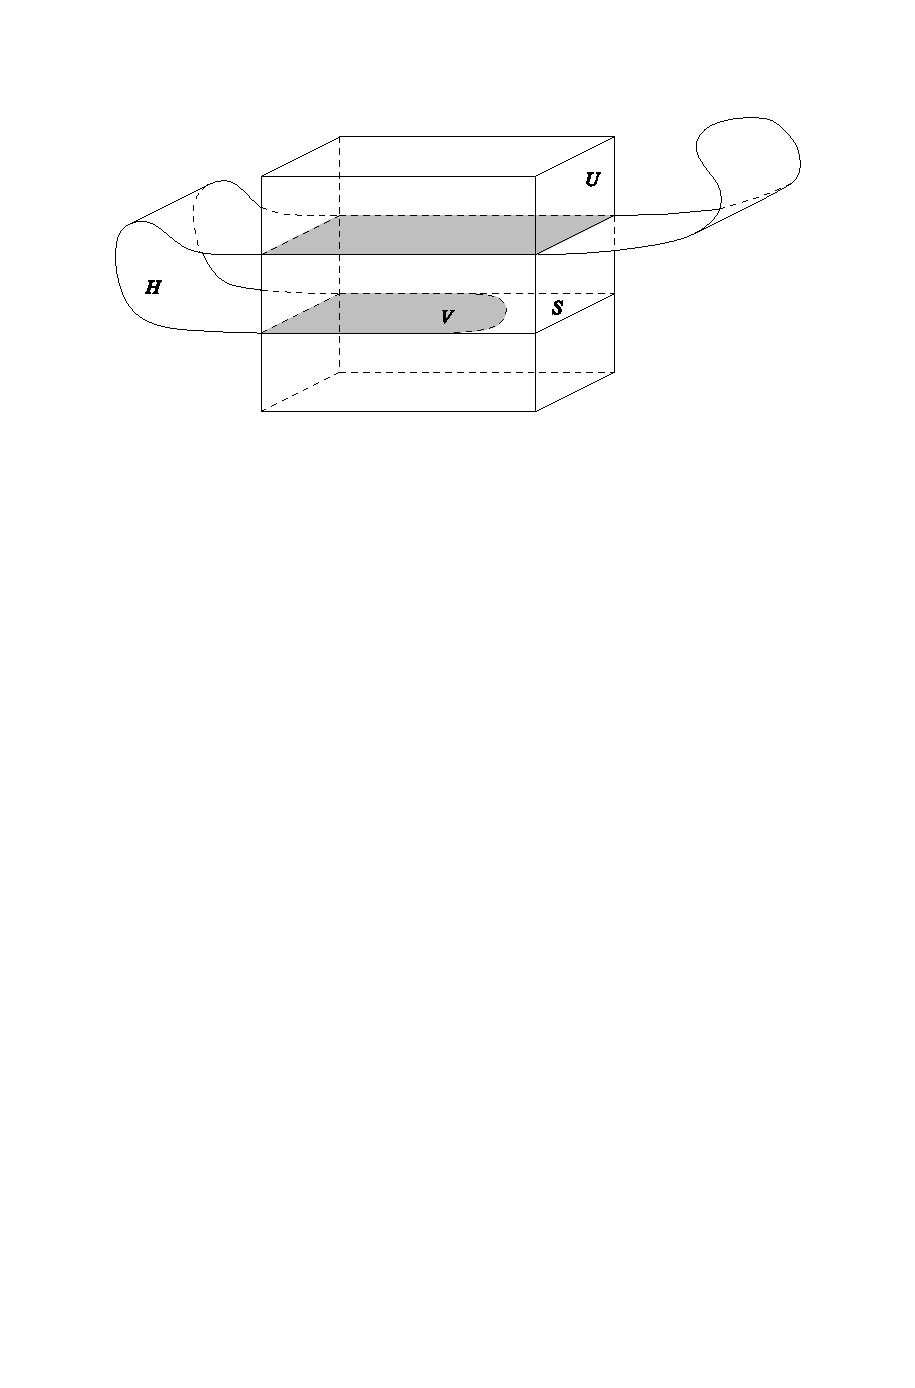
\includegraphics[scale=0.8]{figures/frobenius_2.pdf}
    \caption{Local structure of a leaf in a flat chart. From \cite{Lee}.}
    \label{fig: frobenius2}
\end{figure}


\begin{thm}[{{\cite[Thm.~19.17]{Lee}}} or {{\cite[Prop.~3.5.15]{RS1}}}]\label{thm 19.17 Lee}\label{prop 3.5.15 RS1}
    Every integral manifold of an involutive distribution is weakly embedded.
\end{thm}
\begin{proof}
    Let $N\subset M$ be an integral manifold of an involutive rank-$r$ distribution $D$ on $M$ and let $F:L\to M$ be a smooth map such that $F(L)\subset N$. Choose $p\in L$ and set $m=F(p)\in N$. Let $\{y^i\}_{i=1}^n$ be flat coordinates for $D$ on a neighborhood $U$ of $m$, and let $\{x^i\}$ be smooth coordinates for $L$ on a connected neighborhood $B$ of $p$ such that $F(B)\subset U$. With the coordinate representation of $F$ written as 
    \[y^i=F^i(x),\]
    the fact that $F(B)\subset N\cap U$ means that the functions $F^{r+1},\ldots, F^n$ take on only countably many values. Since $B$ is connected, these coordinate functions are constant, and thus $F(B)$ lies in a single slice $U_{\bf{c}}\subset U$. Because $U_{\bf{c}}\cap N$ is an open subset in $N$ that is embedded in $M$, it follows that $\restr{F}{B}$ is smooth from $B$ into $U_{\bf{c}}\cap N$, and thus by composition, $\restr{F}{B}:B\to U_{\bf{c}}\cap N\hookrightarrow N$ is smooth into $N$.
\end{proof}
\begin{cor}
    Images of the maximal integral curves of a vector field are weakly embedded submanifolds.
\end{cor}




% \begin{rem}
%     The version of the Frobenius theorem proved above is local, i.e.\ integral submanifolds are guaranteed to exist only in small neighborhoods. However, the full version of the Frobenius theorem is much more powerful as it establishes a bijection between smooth integrable distributions and smooth \emph{foliations} of $M$ by maximal integral submanifolds (analogs of maximal integral curves of vector fields). A foliation is a decomposition of $M$ into a disjoint union of immersed submanifolds, called \emph{leaves}, such that every point has a local chart in which the foliation is flat (i.e.~the leaves are just $k$-dimensional hyperplanes of the form $x^{k+1}=c^{k+1},\ldots, x^{n}=c^n$). For a global version of the Frobenius theorem, see \cite[Ch.~19]{Lee} or \cite[\S~3.5]{RS1}.
% \end{rem}


\begin{lem}[{{\cite[Lem.~3.5.14]{RS1}}}]\label{lem 3.5.14 RS1}
    Let $D<TM$ be a smooth distribution on $M$.
    \begin{enumerate}
        \item Let $N_1,N_2\subset M$ be two integral manifolds of $D$. If $N_1\cap N_2\neq \varnothing$ then $N_1\cap N_2$ is open in $N_1$ and $N_2$ and the smooth structures on it induced from either coincide. There is a unique smooth structure on $N_1\cup N_2$ such that $N_1$ and $N_2$ are open submanifolds. W.r.t.~this structure $N_1\cup N_2$ is an integral manifold of $D$.

        \item Let $N\subset M$ be an integral manifold of $D$, let $m\in M$ such that $\dim D_m=\dim N$ and let $(U,\kappa)$ be a local flat chart for $D$ at $m$. If a slice $U_{\bf{c}}$ of $U$ intersects $N$, then $U_{\bf{c}}$ is an integral manifold of $D$ and $N\cap U_{\bf{c}}$ is open and closed w.r.t.~the topology induced from $N$. In particular, the number of slices of $U$ intersecting $N$ is at most countable.  
    \end{enumerate}
\end{lem}
Note that the number of slices of $U$ intersected by $N$ may, in fact, be countably infinite, as is the case with the ``irrational slope'' vector fields $\partial_x+\lambda\partial_y$, $\lambda\in\bbR\setminus\bbQ$, on the torus $\bbR^2\slash \bbZ^2$.
\begin{proof}
\begin{enumerate}
    \item The assertion on $N_1\cup N_2$ follows from that on $N_1\cap N_2$, so it suffices to prove the latter. Let $\dim N_1=\dim N_2=\rank D=r$. Choose a local $r$-frame $\{X_i\}_{i=1}^r$ for $D$ at $m$. Since these vector fields are tangent to $N_i$, they are also local vector fields on $N_i$. Then the flows of these vector fields together generate a local coordinate system on $N_i$, mapping $(-\epsilon,\epsilon)^r$ into an open subset of $N_i$:
    \[\Phi^{(i)}:(-\epsilon,\epsilon)^r\to U\cap N_i,\quad \Phi^{(i)}(\bf{t})\coloneqq F^{X^{(i)}_1}_{t_1}\circ \cdots\circ F^{X^{(i)}_r}_{t_r}(m),\quad i=1,2.\]
    By construction these coordinates will coincide, $\Phi^{(1)}(\bf{t})=\Phi^{(2)}(\bf{t})$ (cf.\ Remark~\ref{rem 3.2.9 RS1}), and therefore their values will cover the same subset $V\subset N_1\cap N_2$ open in both $N_i$'s. W.r.t.~the differentiable structure induced from either $N_i$, $V$ is diffeomorphic to $(-\epsilon,\epsilon)^r$. Since the construction works for any $m\in N_1\cap N_2$, the assertion follows. 

    \item Let $r=\dim N=\dim D_m$. If $N$ intersects a slice $U_{\bf{c}}$, then $U_{\bf{c}}$ contains a point where $\rank D=r$. Then $U_{\bf{c}}$ is an integral manifold of $D$ by dimension-counting. Now assertion 1 implies that $N\cap U_{\bf{c}}$ is open in $N$ and hence in $N\cap U$. Since this holds for all slices intersecting $N$ and since
    \[N\cap U_{\bf{c}}=(N\cap U)\setminus\left(\bigcup_{\bf{c}'\neq \bf{c}}N\cap U_{\bf{c}'}\right),\]
    the intersection $N\cap U_{\bf{c}}$ is also closed in $N\cap U$. It follows that $N\cap U_{\bf{c}}$ is a union of connected components of $N\cap U$. Since the slices are disjoint, this implies that the number of slices which intersect $N$ is at most as large as the number of connected components of $N\cap U$. Since the topology on $N\cap U$ is induced from the manifold $N$, it is second countable, hence the number of connected components is at most countable.
\end{enumerate}
\end{proof}



\begin{thm}[{{\cite[Thm.~3.5.17]{RS1}}}]\label{thm 3.5.17 RS1}
    Let $D$ be an integrable distribution on $M$. For every $m\in M$ there exists a unique integral manifold $N_m$ of $D$ through $m$ which is maximal in the following sense. For every integral manifold $N$ of $D$ such that $N\cap N_m\neq \varnothing$ it holds that $N\subset N_m$, and $N$ is an open submanifold of $N_m$.
\end{thm}
\begin{proof}
    Let $r=\dim D_m$ and define a subset $N_m\subset M$ by taking the union of all integral manifolds of $D$ through $m$. Equip it with the topology generated by the open subsets of these integral manifolds. The onion of all maximal atlases of these manifolds also defines an atlas on $N_m$. By Lemma~\ref{lem 3.5.14 RS1} this atlas is smooth.  One can then show that $N_m$ is second countable (see \cite[Lem.~19.22]{Lee} or \cite[Thm.~1.64]{Warner}). Then $N_m$ is a manifold of dimension $r$. By construction, the local representatives of the inclusion $N_m\hookrightarrow M$ are smooth, hence $N_m$ is a smooth submanifold of $M$. Also by construction, every $\wt{m}\in N_m$ belongs to an integral manifold $N$ through $m$ and $N$ is an open submanifold of $N_m$, so $T_{\wt m}N_m=T_{\wt m}N=D_{\wt m}$, and thus $N_m$ is also an integral manifold through $m$. It has the maximality property stated in the theorem because if some integral manifold $N$ of $D$ intersects $N_m$, then $N\cup N_m$ is also integral and thus already contained in $N_m$. It follows that $N\cap N_m=N$ and hence $N$ is an open submanifold of $N_m$. Uniqueness follows because any two maximal integral manifolds through $m$ would coincide as sets by definition and each of them would be an open submanifold of the other, hence they would also coincide as manifolds.
\end{proof}


\begin{defn}[Foliation]\index{Foliation}
    A foliation of an $n$-dimensional smooth manifold $M$ is a family $\mathcal{N}$ of connected submanifolds of $M$, called the \emph{leaves} of the foliation, such that
    \begin{enumerate}
        \item the leaves are disjoint and $\cup_{N\in\mathcal{N}}N=M$,
        \item for every $m\in M$ there exists a local \emph{flat chart} $(U,\kappa)$ of $M$ satisfying
        \begin{enumerate}[label=(\alph*)]
            \item $\kappa(m)=0$ and $\kappa(U)=(-\epsilon,\epsilon)^n$ for some $\epsilon>0$,
            \item the leaves are invariant under the flows of the local coordinate vector fields $\partial_1,\dots,\partial_r$, where $r$ denotes the dimension of the leaf containing $m$, also called the \emph{rank} of $\mathcal{N}$ at $m$.
        \end{enumerate}
    \end{enumerate}
    A foliation is called \emph{regular} if its rank is constant, and singular otherwise.
\end{defn}



\begin{thm}[Global Frobenius Theorem {{\cite[Prop.~3.5.21]{RS1}}} or {{\cite[Thm.~19.21]{Lee}}}]\label{prop 3.5.21 RS1}\index{Theorem!Global Frobenius}
    The collection of all maximal connected integral manifolds of an involutive distribution $D$ on a smooth manifold $M$ forms a foliation of $M$.
    
    The assignment of the family of maximal integral manifolds to an integrable distribution defines a bijection between smooth integrable distributions on $M$ and smooth foliations of $M$. Regular distributions of rank $r$ thereby correspond to regular foliations of rank $r$.
\end{thm}
\begin{proof}
    Theorem~\ref{thm 3.5.17 RS1} implies that condition 1 of the definition of a foliation is satisfied. The invariance of maximal integral manifolds under the flows of local $D$-valued vector fields lets us generate local flat charts via a composition of the flows (as in Rectification Theorem~\ref{rectification}) and hence condition 2 is satisfied as well. 

    Conversely, let $\mathcal{N}$ be a smooth foliation. For $m\in M$, let $D_m$ be the tangent space at $m$ of the leaf containing $m$. This defines a subset $D\subset TM$. By definition of a foliation, $D_m$ is spanned by the values of local $D$-valued vector fields at $m$. Hence $D$ is a distribution. By construction, every leaf is an integral manifold of $D$. First, this implies that $D$ is integrable. Second, in view of Theorem~\ref{thm 3.5.17 RS1}, this implies that every leaf of $\mathcal{N}$ is contained in an open subset in a maximal integral manifold of $D$. Thus $N$ is a union of leaves. Since the leaves are disjoint and $N$ is connected, $N$ must coincide with a single leaf. This shows that $\mathcal{N}$ is the family of maximal integral manifolds of $D$, and the assignment is bijective, indeed.
\end{proof}



\begin{figure}
    \centering
    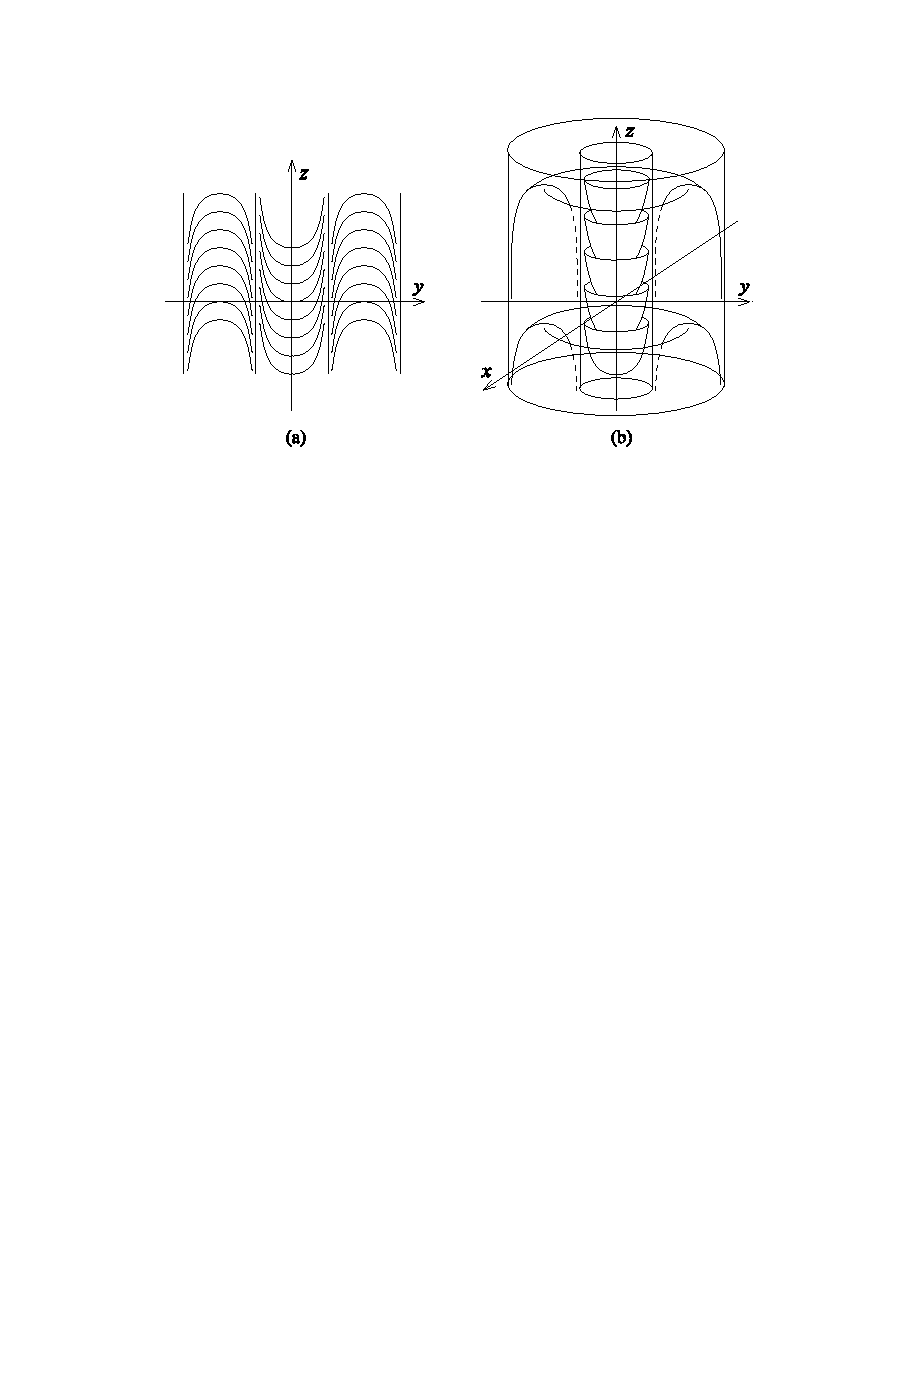
\includegraphics[scale=0.8]{figures/foliations.pdf}
    \caption{Examples of foliations of $\bbR^2$ (a) and $\bbR^3$ (b). From \cite{Lee}.}
    \label{fig:foliations}
\end{figure}

\begin{example}[Linear PDEs]
    Overdetermined systems of linear PDEs are solvable iff the distribution spanned by the differential operators as vector fields is integrable:
    \[\begin{cases}
        X_1\cdot u(x)=f_1(x),&\\
        \cdots &\\
        X_k\cdot u(x)=f_k(x)&
    \end{cases}
    \text{ has solutions iff }\exists\,C^k_{ij}\in C^\infty\text{ s.t.}
    \begin{cases}
        [X_i,X_j]=C^k_{ij}X_k,&\\
        X_i\cdot f_j-X_j\cdot f_i=C^k_{ij}f_k.&
    \end{cases}
    \]
\end{example}

\begin{example}[Zero curvature conditions]\label{ex UV pairs}
    Another important case is the following pair of equations on a function $\bf{y}:\bbR^2\to \bbC^n$ parametrized as $\bf{y}(x,t)$:
    \[\begin{cases}
        \partial_x \bf{y}(x,t)= U(x,t)\bf{y}(x,t),\\
        \partial_t \bf{y}(x,t)= V(x,t)\bf{y}(x,t),
    \end{cases}\label{eq UV pair}\]
    where $U,V:\bbR\times\bbR\to \bbC^{n\times n}$ are given matrix-valued functions. As we will see later, $U$ and $V$ can be seen as the components of a linear connection $U\dd x+V\dd t$ on the product bundle $\bbR^2\times\bbC^n\to \bbR^2$, so that the above equations become $\nabla\bf{y}=0$. The Frobenius integrability condition in this case is easy to obtain by observing that any solution must satisfy $\partial_t(\partial_x \bf{y})=\partial_x(\partial_t \bf{y})$, which expands to 
    \[(\partial_t U+UV)\bf{y}=(\partial_x V+VU)\bf{y},\]
    or (since the initial condition is arbitrary)
    \[\partial_t U-\partial_x V+[U,V]=0.\]
    If this condition holds, then the Frobenius theorem guarantees the unique existence of solutions. This condition is called a \emph{zero curvature condition}, and when a given dynamical system can be expressed in the form of a zero curvature condition, the system~(\ref{eq UV pair}) is called a \emph{$UV$-pair}, and the dynamical system is considered \emph{integrable}.\footnote{However, this is not the only test for integrability, and a general definition of integrability for dynamical systems doesn't exist} We will see its relation to the Maurer-Cartan equation in \subsect\ \ref{subsec: invariant diff forms}.
\end{example}

\begin{example}[Sine-Gordon equation]\label{ex sine-gordon}
    Consider the $UV$-pair (with the variables $x,t$ suppressed)
    \[U(\lambda)=\frac{\rmi}{2}\begin{pmatrix}
        2\lambda & u_x\\
        u_x & -2\lambda
    \end{pmatrix},\quad 
    V(\lambda)=\frac{1}{4\rmi \lambda}\begin{pmatrix}
        \cos u & -\rmi \sin u\\
        \rmi \sin u & -\cos u
    \end{pmatrix},
    \]
    where $u(x,t;\lambda)$ is an $\bbR$-valued function, subscripts stand for partial derivatives of $u$, and $\lambda\neq 0$ is a complex parameter. This $UV$-pair defines a system of equations (\ref{eq UV pair}) on the unknown $\bf{y}$. By expanding the zero curvature condition we find that its diagonal components vanish, and both anti-diagonal components impose the \emph{Sine-Gordon equation}\index{Equation!Sine-Gordon} on $u$:
    \[u_{xt}=\sin u.\]
\end{example}

\begin{example}[AKNS, Nonlinear Schr\"odinger equation]
    Consider now the $UV$-pair 
    \[
    U(\lambda)=-\rmi\lambda
    \begin{pmatrix}
        1 & 0\\
        0 & -1
    \end{pmatrix}+\rmi\begin{pmatrix}
        0 & p\\
        -q & 0
    \end{pmatrix},\quad 
    V(\lambda)=
    2\lambda U(\lambda)
    -\rmi\lambda\begin{pmatrix}
        pq & \rmi p_x\\
        \i q_x & -pq
    \end{pmatrix},\label{eq AKNS UV pair}
    \]
    where $p(x,t;\lambda),q(x,t;\lambda)\in\bbC$. The zero curvature condition then leads to the \emph{AKNS system} on $q$ and $p$:
    \[
        \begin{cases}
            \i p_t+p_{xx}-2p^2q= &0,\\
            -\i q_t+q_{xx}-2q^2p= &0.
        \end{cases}    
    \]
    Under the so called self-adjoint reduction $p=-\wb{q}\eqqcolon \psi$ this system turns into the standard \emph{Nonlinear Schr\"odinger} (NLS) equation on $\psi$, of great importance in optics:\index{Equation!Nonlinear Sch\"odinger}\index{Equation!AKNS}
    \[\rmi\psi_t+\psi_{xx}+2|\psi|^2\psi=0.\]
\end{example}

\begin{example}[Lax pairs]\label{ex Lax pairs}\index{Lax pair}
    Another common way of demonstrating the integrability of a dynamical system is by finding a representation in terms of a \emph{Lax pair},\index{Lax pair} which consists of two matrix-valued operators $L,A$, where $L$ is the linear differential operator
    \[L(t)=u_m(x,t)\partial_x^m+\cdots u_1(x,t)\partial_x+u_0(x,t)\]
    with matrix-valued functions $u_i:\bbR^2\to \bbC^{n\times n}$, and $A$ is another matrix-valued differential (only with respect to $x$) operator such that our dynamical system describing the evolution of $u_i(x,t)$ is expressed as 
    \[L_t=[A,L],\label{eq Lax pair}\]
    where 
    \[L_t=\dot u_m(x,t)\partial_x^m+\cdots \dot u_1(x,t)\partial_x+\dot u_0(x,t),\]
    and $[A,L]$ is computed as the commutator of differential operators acting on smooth functions $\bf{\psi}(x,t)\in\bbC^n$. The core observation here is that the matrices $L(t)$ at different values of $t$ are all similar. That is, $L(t)$ can be written in terms of $L(s)$ as 
    \[L(t)=M(t,s)L(s)M(t,s)^{-1},\]
    where (by plugging into (\ref{eq Lax pair})) $M(t,s)$ satisfies the Cauchy problem 
    \[\partial_t M(t,s)=A(t)M(t,s),\quad M(s,s)=\rmI_n,\]
    where $\rmI_n$ is the identity matrix of size $n\times n$.
    Note that while $M$ will implicitly depend on $x$, the derivatives $\partial_x^j$ contained in $L$ do not act on $M$ in this equation. Therefore, $M$ always exists due to the general solvability of Cauchy problems.

    The main consequence of this is that the eigenvalues of $L(t)$ do not depend on $t$. This is known as the \emph{isospectral property} of Lax pairs. Therefore, to solve the eigenvalue problem $L(t)\bf{\psi}(x,t)=\lambda\bf{\psi}(x,t)$ at time $t$, it suffices to solve it at $t=0$ (where $L$ is usually known better due to the initial condition) and then propagate the solution using the formulas
    \[\begin{cases}
        \lambda(t)=\lambda(0),\\
        L(t)\bf{\psi}=\lambda(t)\bf{\psi},\\
        \partial_t\bf{\psi}=A\bf{\psi}.
    \end{cases}\label{eq Lax pair 2}\]
    Let us now take this system as the starting point and differentiate the second equation with respect to $t$, getting $\dot L\bf{\psi}+L\dot{\bf{\psi}}=\lambda\dot{\bf{\psi}}=\lambda A\bf{\psi}=A L\bf{\psi}$. Substituting $\dot{\bf{\psi}}=A\bf{\psi}$ into the left hand side as well, we get back the Lax equation $\dot L=[A,L]$. Therefore, the Lax equation is the compatibility (or integrability) condition for (\ref{eq Lax pair 2}).

    To see the connection to zero curvature conditions, suppose $L$ and $A$ have the form 
    \begin{align}
        L=\partial_x^n+\sum_{j=0}^{n-1}u_j(x,t)\partial_x^j,\\
        A=\partial_x^n+\sum_{j=0}^{n-1}v_j(x,t)\partial_x^j.
    \end{align}
    Then the isospectral equation $L\bf{\psi}=\lambda\bf{\psi}$ implies that $x$-derivatives of $\bf{\psi}$ of order $\geq n$ may be expressed as linear combinations of derivatives of orders $<n$. Indeed, we have
    \[\partial_x^n\bf{\psi}=\lambda\bf{\psi}-\sum_{j=0}^{n-1}u_j(x,t)\partial_x^j\bf{\psi},\]
    and further differentiations of this equation with respect to $x$ give the higher-order derivatives as well. Now, introducing the vector 
    \[\bf{y}=(\bf{\psi},\partial_x\bf{\psi},\ldots,\partial_x^{n-1}\bf{\psi}),\]
    the equation $L\bf{\psi}=\lambda\bf{\psi}$ can be written as 
    \[\partial_x\bf{y}=U\bf{y},\]
    where 
    \[U(x,t;\lambda)=
    \begin{pmatrix}
        0 & 1 & 0 & \cdots & 0\\
        0 & 0 & 1 & \cdots & 0\\
        \vdots & \vdots & \vdots & \ddots & \vdots \\
        0 & 0 & 0 & \cdots & 1\\
        \lambda-u_0 & -u_1 & -u_2 & \cdots & -u_{n-1}
    \end{pmatrix}.
    \]
    Now let us act with $\partial_x^i$ on the equation $\dot{\bf{\psi}}=A\bf{\psi}$ to obtain 
    \[\partial_t(\partial_x^{i-1}\bf{\psi})+\underbrace{\partial_x^{i-1}\left(\sum_{j=0}^{m-1}v_j(x,t)\partial_x^i\bf{\psi}\right)}_{\sum_{j=1}^nV_{ij}(x,t;\lambda)\partial_x^{j-1}\bf{\psi}}=0,\]
    for some $V_{ij}(x,t;\lambda)$ that can be expressed in terms of $v_j$, $u_i$, and their derivatives of orders $<n$ by our above observation. This equation can be written as 
    \[\partial_t \bf{y}=V\bf{y}.\]
    We have shown the equivalence between Lax representations and zero curvature representations:
    \[
    \dot L=[A,L]\Leftrightarrow 
    \begin{cases}
        L\bf{\psi}=\lambda\bf{\psi},\\
        \partial_t\bf{\psi}=A\bf{\psi}
    \end{cases}\Leftrightarrow
    \begin{cases}
        \bf{y}_x=U\bf{y},\\
        \bf{y}_t=V\bf{y}
    \end{cases}\Leftrightarrow
    \partial_t U-\partial_x V+[U,V]=0.
    \]
\end{example}

\begin{example}
    In many famous examples of Lax pairs, $n=1$ and $L$ is the second-order \emph{Sturm-Liouville operator} (in physics a Schr\"odinger operator)
    \[L=-\partial_x^2+u.\]
    The simplest choice of $A$ is $A=-c\partial_x$ with a constant $c$, which leads to the \emph{1D advection equation}
    \[A=-c\partial_x\quad \Rightarrow \quad u_t+c u_x=0.\]
    The following choice of $A$ leads to the celebrated solitonic \gls{kdv} equation:\index{Equation!Korteweg-de~Vries}
    \[A=-4\partial_x^3+6u\partial_x+3u_x\quad \Rightarrow\quad u_t-6uu_x+u_{xxx}=0.\label{eq kdv}\]
\end{example}


\begin{xca}
    Show that the distribution on $\bbR^3\setminus \{0\}$ generated by the vector fields
    \[X_1=x_2\partial_3-x_3\partial_2,\quad X_2=x_3\partial_1-x_1\partial_3,\quad X_3=x_1\partial_2-x_2\partial_1,\]
    is regular of rank $2$ and involutive. Find the maximal integral manifolds. How are they related to the action of $\SO(3)$ on $\bbR^3$?
\end{xca}











\clearpage
\section{Differential Forms and Integration}

\subsection{Exterior algebra}


\begin{defn}[Exterior forms]\index{Exterior form}
    Let $V$ be a $\bbK$-vector space. The alternation and symmetrization maps are defined on the tensor space $T^k V=(V)^{\otimes k}$ respectively as
    \begin{align}
        \Alt t&=\frac{1}{k!}\sum_{\sigma\in S_k} (\sign\sigma)\cdot t^\sigma,\\
        \Sym t&=\frac{1}{k!}\sum_{\sigma\in S_k} t^\sigma,\label{def sym operator}
    \end{align}
    where $S_k$ is the $k$-th permutation group, and the operation $t\mapsto t^\sigma$ is defined on a basis as $(e_{i_1}\otimes\cdots\otimes e_{i_k})^\sigma=e_{\sigma(i_1)}\otimes\cdots\otimes e_{\sigma(i_k)}$ and extended to all of $T^k V$ by linearity. We also denote $\bigwedge^k V=\Alt(T^k V)$ and $\rmS^k V=\Sym(T^k V)$. Elements of the space $\bigwedge^k V^\ast$ are called \emph{exterior forms} of degree $k$ on $V$. 
    
    If $\dim V=n$, then $\dim \bigwedge^k V=\binom{n}{k}$. In particular, 
    \[\bigwedge^1 V=V,\quad \dim \bigwedge^0 V=\dim \bigwedge^n V=1,\quad \dim \bigwedge^{>n} V=0.\]
    Elements of $\bigwedge^n V$ are called \emph{top forms}.\index{Top form}
    Both $\bigwedge^k$ and $\rmS^k$ are covariant functors $\mathsf{FinVect}_\bbK\to\mathsf{FinVect}_\bbK$ that act on morphisms by restriction: \[\bigwedge^k f=\restr{f^{\otimes k}}{\bigwedge^k V},\quad \rmS^k f=\restr{f^{\otimes k}}{\rmS^k V}.\]
\end{defn}

If $V$ has Cartesian coordinates $x^1,\ldots,x^n$, then a basis of $V$ is formed by $\{\partial_{x^i}\}$. The dual basis of $V^\ast$ is conventionally denoted by $\{\dd x^i\}$, so that
\[
    \dd x^i\left(\partial_{x^j}\right)=\delta^i_j.
\]
Then this basis induces a basis of $\bigwedge^k V^\ast$ consisting of the $\binom{n}{k}$ elements
\[
\dd x^{i_1}\wedge \cdots \wedge \dd x^{i_k}\coloneqq k!\Alt(\dd x^{i_1}\otimes\cdots\otimes \dd x^{i_k}),\;\;1\leq i_1<i_2<\cdots<i_k\leq n.
\]
Together with the wedge product, the direct sum of all exterior powers of $V$ makes up an algebra, called the exterior, or \emph{Grassmann}, algebra of $V$, of dimension $2^n$:\index{Grassmann algebra}
\[\bigwedge V=\bigoplus_{k=0}^\infty \bigwedge^k V.\]



\begin{defn}[Determinant of a linear map]\index{Determinant of a linear map}
Let $V$ be a vector space over a field $\bbK$ with $\dim V=n$ and let $f\in\End(V)$. The determinant of $f$ is defined as 
\[\det f\coloneqq \bigwedge^n f\quad \in\bbK.\] 
Being an element of $\Hom(\bigwedge^n V,\bigwedge^n V)$, which is naturally isomorphic to the field $\bbK$, it is a well-defined scalar. 
\end{defn}
\begin{prop}
\begin{enumerate}
    \item If $\dim V=n$, then for any $t\in\bigwedge^n V^\ast$ and any $f\in\End(V)$, 
    \[f^\ast t=\det f\cdot t.\]
    \item If $f\in\End(V)$ is represented by a matrix $f(e_i)=A_i^j e_j$ in some basis $\{e_i\}$ of $V$, then
    \[\det f=\det A=\sum_{\sigma\in S_n}(\sign\sigma)A^1_{\sigma(1)}\cdots A^n_{\sigma(n)}.\]
\end{enumerate}
\end{prop}
\begin{proof}
\begin{enumerate}
    \item By definition of $f^\ast$, if $v\in \bigwedge^n V$, then 
    \[(f^\ast t)(v)=t\left(f_\ast(v)\right)=t\left(\left(\bigwedge^n f\right)(v)\right)=t(\det f\cdot v)=\det f\cdot t(v).\]
    \item The one-dimensional space $\bigwedge^n V$ is spanned by the element $e_1\wedge \cdots \wedge e_n$. Acting on it, $\det f=\bigwedge^n f$ gives
    \begin{align}
        \left(\bigwedge^n f\right)(e_1\wedge \cdots \wedge e_n)=&k!f^{\otimes n}\circ \Alt (e_1\otimes \cdots \otimes e_n)=\\
        =&k!\Alt(f(e_1)\otimes\cdots\otimes f(e_n))=\notag
        \\
        =&k! \Alt (A^{j_1}_1 \cdots A^{j_n}_n \cdot e_{j_1}\otimes\cdots \otimes e_{j_n})=\\
        =&\sum_{\pi\in S_n}(\sign\pi)\cdot A_{\pi(1)}^{j_1}\cdots A_{\pi(n)}^{j_n}\cdot  e_{j_1}\otimes\cdots\otimes e_{j_n}=\notag
        \\
        =\sum_{\sigma,\pi\in S_n}(\sign\sigma\cdot\sign\pi) \cdot &A_{\pi(1)}^1\cdots A_{\pi(n)}^n\cdot e_{\sigma(1)}\otimes\cdots\otimes e_{\sigma(n)}=\notag
        \\
        =&\left(\sum_{\pi\in S_n}(\sign\pi)A^1_{\pi(1)}\cdots A^n_{\pi(n)}\right)\cdot e_1\wedge \cdots \wedge e_n.
    \end{align}
    By item 1, the expression in the brackets is the determinant.
\end{enumerate}
\end{proof}

\begin{defn}[Exterior/wedge product]\index{Exterior product}\index{Wedge product| see {Exterior product}}
    For $\alpha\in V^{\otimes p}$ and $\beta\in V^{\otimes q}$, we define their exterior/wedge product by
    \[\alpha\wedge\beta\coloneqq\frac{(p+q)!}{p!q!}\Alt (\alpha\otimes \beta)\quad \in \bigwedge^{p+q}V.\]
\end{defn}
Wedge products have the following basic properties (proofs of which are left as exercises):
\begin{enumerate}
    \item $\alpha\wedge\beta=\Alt(\alpha)\wedge\beta=\alpha\wedge\Alt(\beta)$;
    \item $\wedge$ is bilinear and $\alpha\wedge\beta=(-1)^{\deg\alpha\cdot\deg\beta}\beta\wedge\alpha$;
    \item $\alpha\wedge(\beta\wedge\gamma)=(\alpha\wedge\beta)\wedge\gamma$.
    \item The notation for basis elements is consistent with the definition of the wedge product:
    \[(\dd x^{i_1}\wedge\cdots\wedge \dd x^{i_p})\wedge (\dd x^{i_{p+1}}\wedge\cdots\wedge \dd x^{i_{p+q}})=\dd x^{i_1}\wedge\cdots\wedge \dd x^{i_{p+q}}.\]
    \item For $\alpha_i\in V^\ast$, $i=1,\ldots,k$, 
    \begin{multline}
        (\alpha_1\wedge\cdots\wedge\alpha_k)(v_1,\ldots,v_k)=\sum_{\sigma\in S_k}(\sign\sigma)\cdot \alpha_1(v_{\sigma(1)})\cdots\alpha_k(v_{\sigma(k)})=\\=\det \begin{bmatrix}
         \alpha_1(v_1) & \cdots & \alpha_1(v_k)  \\
         \vdots & \ddots & \vdots \\
         \alpha_k(v_1) & \cdots & \alpha_k(v_k) 
    \end{bmatrix}.\label{form determinant f-la}
    \end{multline}
    \item $\{\alpha_i\}_{i=1}^k\subset V^\ast$ are linearly dependent iff $\alpha_1\wedge\cdots\wedge\alpha_k=0$.
    \item For $\alpha,\beta\in\bigwedge^{\smbullet } V^\ast$ and any linear map $f:V'\to V$,
    \[f^\ast(\alpha\wedge\beta)=(f^\ast\alpha)\wedge(f^\ast\beta).\label{pullbacks of wedges}\]
\end{enumerate}

The degree of an exterior form can be lowered by substituting a given vector as one of its arguments, which we use to define an operator.

\begin{defn}[Inner product]\index{Inner product}
    Let $\alpha\in\bigwedge^{p+1}V^\ast, p\geq 0,$ and $v\in V$. The inner product with $v$ is the operator $i_v:\bigwedge^{p+1}V^\ast\to \bigwedge^p(v)$ defined by 
    \[(i_v \alpha)(v_1,\ldots,v_p)=\alpha(v,v_1,\ldots,v_p),\]
    for $v_1,\ldots,v_p\in V$. We also put $\restr{i_v}{\bigwedge^0V^\ast}=0$.
\end{defn}

Note that $i_v$ is a ``\emph{$\wedge$-derivation}'' on the exterior algebra (exercise):
\[i_v(\alpha\wedge\beta)=i_v\alpha\wedge\beta+(-1)^{\deg \alpha}\alpha\wedge i_v\beta.\label{eq inner product derivation}\]





\begin{comment}
    \begin{samepage}
        \PRLsep
        \begin{center}
            {\red Lecture 15 on 15 Mar 2019 ended here}
        \end{center}
    \end{samepage}
\end{comment}


\begin{defn}[Exterior powers of \glspl{vb}]
Following the logic of Definition \ref{functors VB}, we can extend the functors $\bigwedge^p$ and $\rmS^p$ to all smooth \glspl{vb}. We focus only on $\bigwedge^p$. For a \gls{vb} $E\overset{\pi}{\to} M$, we obtain the exterior powers
\[\bigwedge^p E=(E)^{\otimes p}_{\text{asym.}}.\]
$p$ is called the \emph{degree} of the elements or sections of $\bigwedge^p E$: \[\deg \alpha=p\;\text{ for }\;\alpha\in\Gamma^\infty\left(\bigwedge^p E\right).\]
The wedge product $\wedge$ gets extended to sections of these bundles fiberwise.
In particular, if $\rank E=k$, then \[\det E\coloneqq \bigwedge^k E\] is called the \emph{determinant (line) bundle}\index{Determinant bundle} of $E$. If the transition functions of $E$ are $\tau_{\alpha\beta}:U_{\alpha\beta}\to \GL_k(\bbR )$, then the transition functions of $\det E$ are $\det \tau_{\alpha\beta}$.

The alternation and symmetrization maps get extended to $\Alt: E^{\otimes p}\to \bigwedge^p E$ and $\Sym: E^{\otimes p}\to \rmS^p E$.
\end{defn}

All properties of wedge products listed above immediately generalize to sections of the exterior bundles.

\begin{defn}[Determinant of a \gls{vb} morphism]
If $E\overset\pi\to M$ is a \gls{vb} of rank $k$ and $f:E\to E$ is a bundle map, then we define $\det f=\bigwedge^k f$. If $\omega\in\Gamma^\infty(\det E^\ast)$, then $f^\ast \omega=\det f\cdot \omega$.
\end{defn}

\begin{defn}[Exterior/Grassmann algebra]\index{Exterior algebra}\index{Grassmann algebra|see {Exterior algebra}}
For a \gls{vb} $E$, the space $\bigoplus_{p\geq 0}\Gamma^\infty(\bigwedge^p E)=\Gamma^\infty\left(\bigoplus_{p\geq 0}\bigwedge^p E\right)$ with the product $\wedge$ is called the exterior, or Grassmann, algebra of $E$.
\end{defn}

% \begin{xca}
%     \begin{enumerate}
%         \item Prove formula \ref{form determinant f-la}.
%         \item Show that $k$ one-forms (or vectors) $\{\alpha_i\}$ are linearly independent iff $\alpha^1\wedge\cdots\wedge\alpha^k\neq 0$. 
%     \end{enumerate}
% \end{xca}






\subsection{Cartan's calculus}

We now move from arbitrary bundles to manifolds by applying the exterior power functor to the tangent bundle.

\begin{defn}[Differential forms]\index{Differential form}
    Differential forms of degree $p$ on a smooth manifold $M$ are sections of $\bigwedge^p (T^\ast M)$. The exterior algebra of differential forms is denoted
    \[\Omega^p(M)\coloneqq \Gamma^\infty\left(\bigwedge^p(T^\ast M)\right),\quad 0\leq 0\leq\dim M.\]
    For $p<0$ and $p>\dim M$ we set $\Omega^p(M)=\{0\}$.
    In particular, we have $\Omega^0(M)=C^\infty(M)$, $\Omega^1(M)=\fX^\ast (M)$, and $\Omega^p(M)\cong \bigwedge^p \fX^\ast(M)$ by Theorem~\ref{thm tensor characterization}. We also denote the \emph{exterior algebra} of $M$ by
    \[\Omega^{\smbullet}(M)\coloneq\bigoplus_{p=0}^{\dim M} \Omega^p(M).\]
    Note that elements of $\Omega^{\smbullet}(M)$ can have mixed degrees, i.e.\ contain terms that are differential forms of differing degrees.
\end{defn}


\begin{rem}
    Since differential forms are covariant tensor fields, they can be expanded in local coordinates $(U,\bf{x})$ as combinations of terms of the form $\dd x^{i_1}\otimes\cdots\otimes \dd x^{i_p}$ with coefficients in $C^\infty(U)$. By taking into account the antisymmetry of forms, we conclude that every differential form $\omega\in\Omega^p(M)$ has the following coordinate representation, where $n=\dim M$:
    \[\omega=\sum_{1\leq i_1<\cdots <i_p\leq n}\omega_{i_1 i_2\cdots i_p}\dd x^{i_1}\wedge\cdots\wedge \dd x^{i_p},\quad \omega_{i_1 i_2\cdots i_p}\in C^\infty(U).\label{eq local rep of a p-form}\]
\end{rem}


Recall that for $f\in C^\infty(M)$, $\dd f=\pr_2\circ f_\ast$, where $\pr_2$ is the projection onto the fiber in $T\bbR =\bbR \times\bbR $. As we have established in Example \ref{df is a one-form}, using the tensor characterization theorem, the differential is a one-form, $\dd f\in\Omega^1(M)$. We can now verify that our notation for the coframe $\{\dd x^i\}_{i=1}^n$ is consistent with the action of $\dd$ on the coordinate functions $x^i$.

\begin{prop}
    If $x^i\in C^\infty(U),i=1,\ldots,n$ are local coordinate functions on $U\subset M$, then the differentials $\dd x^i$ of these functions coincide with the dual coordinate frame, i.e.
\[\dd x^i(\partial_j)=\delta^i_j.\]
\end{prop}
\begin{proof}
    Recall that $x^i_\ast$ are exactly the components of the bundle chart for $TM$. Therefore $x^i_\ast(\partial_j)=(\partial_j)^i$ and
    \[\dd x^i(\partial_{j})=\pr_2\circ x^i_\ast (\partial_{j})=(\partial_j)^i=\delta^i_j.\]
    Equivalently, by definition of the Lie derivative, 
    \[\dd x^i(\partial_j)=\Lie_{\partial_j}x^i=\frac{\partial x^i}{\partial x^j}=\delta^i_j.\]
\end{proof}
\begin{cor}
    Locally, the differential $\dd f$ of a function $f\in C^\infty(M)$ is the standard ``total differential'' from multivariable calculus, \[\dd f=\dd f(\partial_i)\cdot\dd x^i=(\partial_i f)\cdot \dd x^i.\]
\end{cor}

\begin{xca}
    On $\bbR^2$ with Cartesian coordinates $(x,y)$, compute $(\dd x\wedge \dd y)(\nabla f,\nabla g)$ for any $f,g\in C^\infty(\bbR^2)$. Compare to $(\dd f\wedge \dd g)(\partial_x,\partial_y)$ and $(\partial_x\wedge\partial_y)(\dd f,\dd g)$ (where we act with vectors on covectors via the canonical pairing between $TM$ and $T^\ast M$).
\end{xca}

\begin{thm}\label{exterior d existence}
    There exists a unique family of differential operators $\wt{\dd}_p(U):\Omega^p(U)\to \Omega^{p+1}(U)$ for every $U\mathring\subset M$, denoted collectively by $\wt\dd$, such that:
\begin{enumerate}
    \item $\wt\dd$ is an $\bbR $-linear $\wedge$-derivation: $\wt\dd(\alpha\wedge\beta)=\wt\dd\alpha\wedge\beta+(-1)^{\deg\alpha}\alpha\wedge\wt\dd\beta$;
    \item $\forall f\in C^\infty(M)$, $\wt\dd f=\dd f$;
    \item $\wt\dd\circ\wt\dd=0$;
    \item $\wt\dd$ is local: $\wt\dd\left(\restr{\alpha}{U}\right)=\restr{\wt\dd\alpha}{U}$.
\end{enumerate}
\end{thm}
\begin{proof}
Suppose the existence of $\wt\dd$ is established. Then let us consider its action on differential forms of the form $f_0\cdot \dd f_1\wedge \cdots \wedge \dd f_p$ where $f_i\in C^\infty(M)$ (such forms span the entire space $\Omega^p(M)$). Using the properties (1)-(3), we find
\[\wt\dd (f_0\cdot \dd f_1\wedge \cdots \wedge \dd f_p)\overset{(1),(3)}{=}(\wt\dd f_0) \wedge \dd f_1\wedge \cdots \wedge \dd f_p\overset{(2)}{=}(\partial_i f_0)\cdot \dd x^i\wedge \dd f_1\wedge \cdots \wedge \dd f_p.\]
This formula in fact completely determines the action of $\wt\dd$ on all differential forms! Namely, if locally $\omega$ is expressed as (\ref{eq local rep of a p-form}), then
\[\wt\dd \omega =\sum_{i_0=1}^n\sum_{1\leq i_1<\cdots <i_p\leq n}\partial_{i_0}\omega_{i_1 i_2\cdots i_p}\cdot \dd x^{i_0}\wedge \dd x^{i_1}\wedge\cdots\wedge \dd x^{i_p}.\label{eq local formula for d}\]
This formula is in fact coordinate-independent and therefore defines a true differential operator on the algebra of differential forms. All four properties immediately follow (Exercise; only property 3 is nontrivial). This proves the existence and uniqueness.
\end{proof}

\begin{defn}[Exterior derivative]\index{Exterior derivative}
    The differential operator whose existence and uniqueness is established in Theorem~\ref{exterior d existence} is called the exterior derivative of differential forms and is denoted just $\dd:\Omega^p(M)\to\Omega^{p+1}(M)$.

    A differential form $\omega\in\Omega^p(M)$ is called \emph{closed} if $\dd\omega=0$ and \emph{exact} if $\omega=\dd\eta$ for some $\eta\in\Omega^{p-1}(M)$. \index{Closed form}\index{Exact form}
\end{defn}

The following proposition shows that $\dd$ is natural with respect to smooth maps. This property is often described as ``differentials are invariant under changes of variables''.

\begin{prop}
    If $F\in C^\infty(M,N)$, then $F^\ast:\Omega^{\smbullet }(N)\to\Omega^{\smbullet }(M)$ is a homomorphism of algebras and
    \[F^\ast \dd\omega=\dd F^\ast\omega.\]
\end{prop}
\begin{proof}
    The homomorphism part follows from (\ref{pullbacks of wedges}). The second part can be checked in local coordinates using the homomorphism property. First, for $f\in C^\infty(N)$, we have $F^\ast f=f\circ F$, and using Proposition \ref{pullbacks of Lie derivatives} (note that $F$ doesn't have to be a diffeomorphism here because we only need to push $X_m$ at a single point $m\in M$ \emph{forward}), we find
    \[(F^\ast \dd f)(X)(m)=\dd f(F_\ast X_m)=(F^\ast \Lie_{F_\ast X}f)(m)=(\Lie_X F^\ast f)(m)=(\dd F^\ast f)(X)(m),\label{137964}\]
    next we can apply this to every term in a local expansion (\ref{eq local rep of a p-form}) of a differential form $\omega\in\Omega^p(N)$:
    \[F^\ast(\dd\omega)=F^\ast(\dd\omega_{i_1\cdots i_p}\wedge \dd x^{i_1}\wedge\cdots \wedge \dd x^{i_p})=(F^\ast\dd\omega_{i_1\cdots i_p})\wedge F^\ast \dd x^{i_1}\wedge\cdots\wedge F^\ast \dd x^{i_p}.\]
    But each instance of $\dd$ in this expression commutes with $F^\ast$ according to (\ref{137964}), so we get $\dd F^\ast\omega$.
\end{proof}

\begin{rem}
    The proof above explains how pullbacks work in practice. If a differential form is expressed in terms of products of the $1$-forms $\dd x^i$, then $F^\ast\dd x^i$ is simply $\dd (x^i\circ F)$, i.e.\ we merely substitute the values of $F$ into the basic differentials $\dd x^i$.
\end{rem}

\begin{example}
    \begin{enumerate}
        \item If $f\in C^\infty(\bbR)$, written as $y=f(x)$, then $f^\ast \dd y=\dd f(x)=f'(x)\dd x$.
        \item If $F$ is injective, then $F^\ast\omega$ can be viewed as a ``restriction'' of $\omega$ to the image of $F$. For example, if $F:\bbR^2\to \bbR^3$ is an immersion defining a surface $S<\bbR^3$ parametrized via $F(u,v)=(F^1(u,v),F^2(u,v),F^3(u,v))$, then 
        \begin{multline}
            F^\ast(\dd x^1\wedge\dd x^2)=\dd F^1\wedge\dd F^2=(\partial_u F^1\dd u+\partial_v F^1\dd v)\wedge(\partial_u F^2\dd u+\partial_v F^2\dd v)=\\=(\partial_u F^1\partial_vF^2-\partial_uF^2\partial_vF^1)\dd u\wedge\dd v.
        \end{multline}
        Since every vector tangent to $S$ can be expressed as the push-forward by $F$ of some vector in $\bbR^2$, this formula essentially expresses the action of the $2$-form $\dd x^1\wedge\dd x^2\in\Omega^2(\bbR^3)$ on pairs of such vectors in local coordinates $(u,v)$ for the surface. In this sense, this is nothing but the restriction of  $\dd x^1\wedge\dd x^2$ to vectors tangent to this surface.
    \end{enumerate}
\end{example}


\begin{cor}
    $\Omega:\mathsf{Man}^\infty \to\mathsf{Alg}$ is a functor, and in fact it is a functor into the category of graded-commutative differential algebras.\footnote{A graded-commutative algebra is an algebra that can be decomposed as a direct sum of vector spaces, $A=\bigoplus_{p\geq 0}A_p $, such that the product acts as $\wedge:A_p\times A_q\to A_{p+q}$ and $\omega\wedge\eta=(-1)^{\deg\omega\cdot\deg\eta}\eta\wedge\omega$. It is also called differential if there is a distinguished graded $\wedge$-derivation $\dd:A_p\to A_{p+1}$ such that $d\circ d=0$.}
\end{cor}

\begin{defn}[Inner product]\index{Inner product}
Let $\omega\in\Omega^{p+1}(M), p\geq 0,$ and $X\in\fX(M)$. The inner product with $X$ is the operator $i_X:\Omega^{p+1}(M)\to \Omega^p(M)$ defined by 
\[(i_X \omega)(X_1,\ldots,X_p)=\omega(X,X_1,\ldots,X_p).\]
We also put $\restr{i_X}{\Omega^0(M)}=0$.
\end{defn}


\begin{prop} For any $X\in\fX(M)$ and any $\omega\in\Omega^{\smbullet }(M)$,
\begin{enumerate}
    \item $\dd\Lie_X=\Lie_X\dd$ on $\Omega^{\smbullet }(M)$;
    \item $i_X$ is a $\wedge$-derivation on the exterior algebra;
    \item $i_{f\cdot X}=f\cdot i_X$;
    \item $i_X\dd f=\Lie_X f$ for $f\in \Omega^0(M)$;
    \item $\restr{\Lie_X}{\Omega^p(M)}=i_X\circ\dd+\dd\circ i_X$ (Cartan's magic formula);\index{Equation!Cartan's magic}
    \item $\Lie_{fX}\,\omega=f\Lie_X\omega +\dd f\wedge i_X\omega$;
    \item For any diffeo $F$, $F^\ast i_X\omega =i_{F^\ast X}F^\ast\omega$.
\end{enumerate}
\end{prop}
\begin{proof}
\begin{enumerate}
    \item First we check that the Lie derivative of a differential form is a differential form. It suffices to check the property on differential forms of the form $\alpha^1\wedge\cdots\wedge\alpha^p$, $\alpha^i\in\Omega^1(M)$. We know that $\Lie_X$ is a tensor derivation, so 
    \[\Lie_X (\alpha^1\wedge\cdots\wedge\alpha^p)=\sum_{i=1}^p \alpha^1\wedge\cdots\wedge\alpha^{i-1}\wedge(\Lie_X\alpha^i)\wedge\alpha^{i+1}\wedge\cdots\wedge\alpha^p.\label{17932121}\]
    Since $\Omega^1(M)=\fX^\ast(M)$, we know that $\Lie_X \alpha^i$ are also one-forms, and thus (\ref{17932121}) is a differential form.
    Furthermore, if $F$ denotes the flow of $X$, then $\Lie_X\alpha (p)=\restr{\frac{\dd}{\dd\lambda}}{\lambda=0}F^\ast_\lambda \alpha$. But we already know that $\dd$ commutes with pullbacks $F^\ast_\lambda$, so the result follows;
    \item Follows from (\ref{eq inner product derivation});
    \item Follows from the linearity of $i_X$;
    \item This is just the definition of $\Lie_X$;
    \item We prove by induction in $p=\deg\omega$. The case $p=0$ reduces to part (4). Any $(p+1)$-form can be locally represented as $\sum_i \dd f_i\wedge \omega_i$ with $f_i\in\Omega^0(U), \omega_i\in \Omega^p(U)$. Thus, we need to check the property only for $\dd f\wedge \omega$. Since $\Lie_X$ is a derivation of the tensor algebra, we have
    \[\Lie_X(\dd f\wedge\omega)=\Lie_X \dd f\wedge \omega+\dd f\wedge \Lie_X\omega.\]
    Now, working backwards,
    \begin{multline}
        i_X\dd (\dd f\wedge \omega)+ \dd i_X (\dd f\wedge\omega)=-i_X(\dd f\wedge\dd \omega)+\dd\left(i_X\dd f\wedge\omega-\dd f\wedge i_X\omega\right)\overset{(2)}{=}
        \\
        =\cancel{-i_X\dd f\wedge\dd \omega}+\dd f\wedge i_X\dd\omega +\dd \underbrace{i_X \dd f}_{\Lie_X f}\wedge\omega+\cancel{i_X\dd f\wedge\dd \omega}+\dd f\wedge \dd i_X\omega\overset{\text{induction}}{=}
        \\
        =\dd f\wedge \Lie_X\omega +\dd \Lie_X f\wedge \omega\overset{(4)}{=}\Lie_X(\dd f\wedge\omega).
    \end{multline}
    \item Follows immediately from part 5.
    \item Explicit check using the definitions of $i_X$ and $F^\ast$ by acting with both sides on a set of vector fields.
\end{enumerate}
\end{proof}

Corollary~\ref{cor willmore formula} implies
\[(\Lie_X\omega) (X_1,\ldots,X_p)=\Lie_X(\omega(X_1,\ldots,X_p))-\sum_{i=1}^p\omega(X_1,\ldots,[X,X_i],\ldots,X_p).\label{3170}\]
We use this property in the proof of the following useful formula.

\begin{prop}[{{\cite[Prop.~4.1.6]{RS1}}}]\label{prop 4.1.6 RS1}
The following explicit coordinate-independent formula for the exterior derivative holds:
\begin{multline}
    (\dd\omega)(X_0,\ldots,X_{p})=\sum_{i=0}^p \Lie_{X_i}(\omega(X_0,\ldots,\wh{X}_i,\ldots,X_p))+\\+\sum_{0\leq i<j\leq p}(-1)^{i+j}\omega([X_i,X_j],X_0,\ldots,\wh{X}_i,\ldots,\wh{X}_j,\ldots,X_p),
\end{multline}
where hats indicate that the corresponding vector fields are excluded from the list of arguments. In particular, for $\alpha\in\Omega^1(M)$,
\[(\dd\alpha)(X_1,X_2)=X_1\cdot \alpha(X_2)-X_2\cdot\alpha(X_1)+\alpha ([X_1,X_2]).\]
\end{prop}
\begin{proof}
Proof by induction in $p$. For $p=0$, we have already established this formula, $\dd \omega(X_0)=\Lie_{X_0}\omega$.

For $p>0$, $(\dd\omega)(X_0,\ldots )=(i_{X_0}\dd\omega)(X_1,\ldots)=(\Lie_{X_0}\omega-\dd i_{X_0}\omega)(X_1,\ldots)$, and by the induction step at $p-1$, we can expand $\dd i_{X_0}\omega$ and permute the result and use (\ref{3170}) to bring it to the required form.
\end{proof}

\begin{xca}
    \begin{enumerate}
        \item Show that if $f_i\in C^\infty(M),$ $i=1,\ldots,k$ are \emph{functionally dependent}, i.e.\ there exists a $g\in C^\infty(\bbR^n)$ such that $g(f_1,\ldots,f_k)=0$, then $\dd f_1\wedge\cdots\wedge \dd f_k=0$.
        \item What conditions need to be added to make part 1 hold in the reverse direction?
    \end{enumerate}
\end{xca}

The following classical theorem shows that every closed differential form is locally exact, i.e.\ on simply connected domains every closed differential form can be written as the derivative of another form.


\begin{thm}[Poincar\'e Lemma]\index{Lemma!Poincar\'e}
    Let $\omega\in\Omega^p(M)$ with $\dd\omega=0$. Then every point $m\in M$ has an open neigborhood $U\subset M$ and a differential form $\eta\in\Omega^{p-1}(U)$ such that $\dd\eta=\restr{\omega}{U}$.
\end{thm}
\begin{proof}
    Let $(U,\bf{x})$ be a chart on $M$ centered at $m$ such that $\bf{x}(U)=\bbR^n$. Thus we may just assume that $M=\bbR^n$. We consider a deformation retraction $\alpha:\bbR\times\bbR^n\to \bbR^n$ given by $\alpha(t,\bf{x})=\alpha_t(\bf{x})=t\bf{x}$. Let $I\in \fX(\bbR^n)$ be the linear vector field $I(\bf{x})=\bf{x}$. Then $\alpha(\rme^t,\bf{x})=F^I_t(\bf{x})$, where $F^I_t$ is the flow of $I$. For $t>0$ we have 
    \[\frac{\dd}{\dd t}\alpha_t^\ast\omega=\frac{\dd}{\dd t}(F^I_{\ln t})^\ast\omega=\frac{1}{t}(F^I_{\ln t})^\ast \Lie_{I}\omega=\frac{1}{t}\alpha_t^\ast(i_{I}\dd\omega+\dd i_{I}\omega)=\frac{1}{t}\dd\alpha_t^\ast i_{I}\omega.\]
    Note that $T_{\bf{x}}(\alpha_t)=t\rmI_n$, where $\rmI_n$ is the identity matrix. Therefore, for $X_2,\ldots,X_p\in \bbR^n=T_{\bf{x}}(\bbR^n)$,
    \begin{multline}
        (\frac{1}{t}\alpha_t^\ast i_{I}\omega)_{\bf{x}}(X_2,\ldots,X_p)=\frac{1}{t}(i_I\omega)_{t\bf{x}}(tX_2,\ldots,tX_p)=\\
        =\frac{1}{t}\omega_{t\bf{x}}(t\bf{x},tX_2,\ldots,tX_p)=\omega_{t\bf{x}}(\bf{x},tX_2,\ldots,tX_p).
    \end{multline}
    So if $p\geq 1$, the $(p-1)$-form $\frac{1}{t}\alpha^\ast_t i_I\omega$ is well-defined and smooth in $(t,\bf{x})$ for all $t\in\bbR$. Clearly $\alpha^\ast_1\omega=\omega$ and $\alpha^\ast_0\omega=0$, so 
    \[\omega=\alpha_1^\ast\omega-\alpha^\ast_0\omega=\int_0^1\frac{\dd}{\dd t}\alpha_t^\ast\omega\dd t=\int_0^1\dd \left(\frac{1}{t}\alpha_t^\ast i_I\omega\right)\dd t=\dd \left(\int_0^1\frac{1}{t}\alpha_t^\ast i_I\omega\dd t\right).\]
\end{proof}




\subsection{Orientation}

The group $\GL^+_n(\bbR )$ is defined as the connected component of the identity in $\GL_n(\bbR )$, i.e.\ the group of matrices with a strictly positive determinant. In accordance with our examples of $G$-structures in \sect~\ref{sec: fiber morphisms}, an orientation is equivalent to a $\GL_n^+(\bbR)$-structure. For a vector space, this means selecting one of the two orbits of the action $\GL_n^+(\bbR)$ on the set of all frames. Below we provide a slightly more traditional, detailed definition.

\begin{defn}[Orientation on a vector space]\index{Orientation!on a vector space}
Let $V$ be an $n$-dimensional real vector space. Two bases $\{e_i\}$ and $\{e_j'\}$ are said to \emph{fix the same orientation} on $V$ if there exists a matrix $A\in\GL^+_n(\bbR )$ such that $e_i=\sum_{j=1}^n A_i^j e_j'$, $1\leq i\leq n$. The two equivalence classes of like-oriented bases on $V$ form the quotient set $\mathcal{O}(V)$. An orientation on $V$ is a choice of an element $\mu\in\mathcal{O}(V)$. Any basis belonging to the chosen orientation, $\{e_i\}\in\mu$, is called \emph{positively oriented} w.r.t.\ that orientation. Since each basis can be identified with a frame $V\to \bbR^n$, an orientation is equivalent to a $\GL_n^+(\bbR)$-structure on $V$ following Definition~\ref{def S-fibers}.
\end{defn}

Note that even though the set $\calO(V)$ of possible orientations has two elements, there is no way to naturally identify it with the group $\bbZ_2$, because neither of the orientations is distinguished. However, at the level of groups, since $\GL_n(\bbR )\slash\GL^+_n(\bbR )=\bbZ_2$, we have a natural group homomorphism $\vartheta:\GL_n(\bbR )\to \bbZ_2=\{-1,+1\}$ given explicitly by $\vartheta(A)=\sign (\det A)$. The action of the group $\GL(V)$ on the set of bases on $V$ then induces a natural action of the group $\bbZ_2$ on the set $\mathcal{O}(V)$. Namely, if $A\in\GL(V)$ and $\{e_i\}$ is a basis, then $\{A\cdot e_i\}$ is oriented like $\{e_i\}$ if $\vartheta(A)=1$, and it has the opposite orientation if $\vartheta(A)=-1$. Therefore, the generator of the group $\bbZ_2$ simply swaps the two elements of $\mathcal{O}(V)$.

Note that any \emph{linear isomorphism} $f:V\to V'$ induces a map $\mathcal{O}(f):\mathcal{O}(V)\to\mathcal{O}(V)$, namely $\mathcal{O}(f)(\mu)=\mu'$ if for any basis $\{e_i\}\in\mu$ the basis $\{f(e_i)\}$ belongs to $\mu'$. Therefore we have constructed a partial covariant functor $\mathcal{O}:\mathsf{FinVect}_\bbR \to\mathsf{2Set}$, where $\mathsf{2Set}$ is the category of two-element sets.

\begin{defn}[Orientation-preserving linear maps]
Let $(V,\mu)$ and $(V,\mu')$ be two oriented vector spaces of equal dimensions. A linear isomorphism $f:V\to V'$ is called orientation-preserving if it maps any positively oriented basis on $V$ to a positively oriented basis on $V'$, i.e.\ it is an isomorphism and $\mathcal{O}(f)(\mu)=\mu'$.
\end{defn}


\begin{defn}[Orientation bundle]\index{Orientation!bundle}
    Let $E\overset\pi\to M$ be a real vector bundle with the typical fiber $F$. The orientation bundle of $E$ is the double cover $\mathcal{O}(E)\overset{\pi}\to M$ (i.e.\ a \gls{fb} whose typical fiber consists of two points) obtained by the application of the smooth functor $\mathcal{O}$ fiberwise as in Definition \ref{functors VB}. Namely, if $\tau_{\alpha\beta}:U_{\alpha\beta}\to\GL(F)$ is a cocycle of $E$, then a cocycle of $\mathcal{O}(E)$ is $\vartheta\circ\tau_{\alpha\beta}=\sign\det\tau_{\alpha\beta}:U_{\alpha\beta}\to\bbZ_2$.
\end{defn}

\begin{xca}
    Show that the orientation bundle of the M\"obius band is isomorphic (as a fiber bundle) to the connected double cover of the circle.
\end{xca}

\begin{defn}[Orientation on a bundle, orientation-preserving maps]\index{Orientation!of a bundle}\index{Orientation!of a manifold}\index{Orientation-preserving maps}
    A real vector bundle $E\overset\pi\to M$ is called orientable if its orientation bundle $\mathcal{O}(E)$ is trivial. An orientation on such a bundle is a choice of one of the two connected components of $\mathcal{O}(E)$. A manifold $M$ is called orientable if its tangent bundle $TM$ is orientable. An orientation on $M$ is an orientation on $TM$.

    A \gls{vb} morphism $f:E\to E'$ between two oriented bundles, such that $f$ restricted to each fiber of $E$ is a linear isomorphism, is called \emph{orientation-preserving} if it preserves the orientation of every fiber. A local diffeomorphism $f:M\to N$ between manifolds of equal dimension is called orientation-preserving if $f_\ast:TM\to TN$ is.
\end{defn}

\begin{prop}\label{prop orientation}
\gls{tfae}:
\begin{enumerate}
    \item A real \gls{vb} $E\overset\pi\to M$ is orientable;
    \item There exists a global section of the orientation bundle $\mathcal{O}(E)$;
    \item The determinant line bundle $\det E$ is trivial;
    \item There exists a non-vanishing section of the determinant line bundle $\det E$;
    \item There exists a bundle atlas on $E$ such that the corresponding cocycle $\{\tau_{\alpha\beta}\}$ has $\det\tau_{\alpha\beta}>0$, i.e.\ if the structure group of $E$ can be reduced to $\GL^+_k(\bbR )$.
\end{enumerate}
\end{prop}
\begin{proof}
    Exercise.
\end{proof}

\begin{xca}
\begin{enumerate}
    \item Show that the M\"obius band is non-orientable as a line bundle over the circle.
    \item Show that the M\"obius band is non-orientable as a manifold.
\end{enumerate}
\end{xca}

\begin{xca}
\begin{enumerate}
    \item Show that the tangent bundle $TM$ of \emph{any} manifold is orientable as a manifold.
    \item Show that any parallelizable manifold is orientable.
    \item Show that an orientable \gls{vb} over an orientable base is orientable as a manifold. Give an example of the converse not being true.
\end{enumerate}
\end{xca}

Since $\GL^+_n(\bbR)$ can be deformation retracted onto $\SL_n(\bbR)$, each orientable vector bundle $E$ admits an atlas in which transition functions are unimodular. A choice of such a reduction is equivalent to picking a nowhere vanishing section $\sfv$ of the dual determinant line bundle $\det E^\ast$. Values $\sfv_m$ of this section can be naturally paired with frames $\{e_i\}_{i=1}^k$ on fibers of $E$ to give a nonzero number $\sfv_m(e_1,\ldots,e_k)$. This induces a notion of a signed volume on each fiber, and in particular an orientation: the frame $\{e_i\}_{i=1}^k$ is positively oriented iff $\sfv_m(e_1,\ldots,e_k)>0$.

\begin{defn}[Volume form]\index{Volume form}
    A volume form on a real \gls{vb} $E\overset{\pi}{\to} M$ is a nowhere vanishing section $\sfv$ of the line bundle $\det E^\ast$. 

    Applying this to the tangent bundle, a volume form on an $n$-dimensional manifold $M$ is a nowhere vanishing differential form of the top degree $\sfv\in \Omega^n(M)$. Given an orientation on $M$, $\sfv$ is called \emph{positive} if for any positively oriented local frame $\{e_i\}$ one has $\sfv(e_1,\ldots,e_n)>0$.
\end{defn}

\begin{prop}
\begin{enumerate}
    \item A manifold $M$ is orientable iff there exists a volume form on $M$;
    \item A choice of a volume form naturally induces a choice of an orientation;
    \item Two volume forms $\sfv,\sfv'$ on $M$ fix the same orientation iff there exists $f\in C^\infty(M)$ such that $f>0$ everywhere and $\sfv=f\cdot \sfv'$. 
\end{enumerate}
\end{prop}
\begin{proof}
Exercise.
\end{proof}


\begin{defn}
Let $M$ and $M'$ be oriented smooth manifolds with chosen volume forms $\sfv$, $\sfv'$, respectively. For a smooth map $f:M\to M'$, we define its determinant with respect to these volume forms by the equality
\[f^\ast \sfv'=\left(\det_{\sfv,\sfv'}f\right)\cdot \sfv.\]
We will usually suppress the dependence on the volume forms. Clearly $f$ is orientation-preserving iff $\det f>0$ everywhere, and $f$ is a local diffeomorphism iff $\det f\neq 0$.

This determinant is still multiplicative: $\det(f\circ g)(p)=(\det f)(g(p))\cdot \det g(p)$.
\end{defn}

\begin{defn}[Tensor densities]\label{def tensor densities}
One can generalize the notion of a tensor field in the following way. Let $w\in\bbZ$ and consider the bundle $(\det M)^{\otimes w}$, where a negative power means $(\det M)^{\ast\otimes |w|}$. Then the sections of the bundle $T^r_s M\otimes (\det M)^{\otimes w}$ (it has the same rank as $T^r_s M$) are called \emph{tensor densities}\index{Tensor density} of weight $w$. An alternative definition uses the bundle $\left|\det M\right|^{w}$ whose transition functions are $|\det\tau_{\alpha\beta}|^w$ if $\tau_{\alpha\beta}$ are the transition functions of $TM$, and $w$ in this case can be any real number $w\in\bbR $. In addition, one can introduce ``pseudotensor densities'' whose transition functions include $(\sign\det\tau_{\alpha\beta})\cdot |\det\tau_{\alpha\beta}|^w$.\index{Pseudotensor density}\index{Density}
\end{defn}

\begin{thm}\label{thm orientation via normal vector}
Let $S<M$ be an immersed submanifold of $\codim S=1$, let $N\in\Gamma^\infty\left(\restr{TM}{S}\right)$ be a section such that $N\not\parallel S$ everywhere, and let $M$ be oriented. Then there exists a unique orientation on $S$ such that a frame $(e_1,\ldots,e_{n-1})$ is positively oriented in $TS$ iff $(N,e_1,\ldots,e_{n-1})$ is oriented in $\restr{TM}{S}$.
\end{thm}
\begin{proof}
Let $\sfv$ be a positive volume form on $M$. The it is easy to check that $\sfv_S\coloneqq i_N \sfv$ is a volume form on $S$ that defines an orientation as stated.
\end{proof}
\begin{cor}
Let $M$ be orientable and let a function $f\in C^\infty(M)$ have a regular value $c\in \bbR $. Then the submanifold $S=f^{-1}(c)\sub M$ is orientable.
\end{cor}
\begin{proof}
Embed $M$ into $\bbR^n$ using the Whitney Embedding Theorem~\ref{thm whitney embedding} and define the vector field $N=\nabla f$. Then $N\perp S$ and $N\neq 0$ on $S$ because $\restr{f}{S}$ is regular. Therefore $N$ induces an orientation on $S$ by the theorem above.
\end{proof}
\begin{cor}
The boundary $\partial M$ of any orientable manifold with boundary is orientable. The standard orientation is fixed by outward normals.
\end{cor}
\begin{proof}
Consider a collar neighborhood of $\partial M$ and the outward vector field $N$ on it. $N$ thus induces an orientation on $\partial M$. This orientation is independent of the choice of $N$ because its $n$-th component at the boundary is necessarily negative and is the only variable between different choices of $N$.
\end{proof}


\begin{defn}[Divergence of a vector field]\index{Divergence}
Let $\sfv$ be a volume form on $M$ and $X\in \fX(M)$. The divergence of $X$ with respect to $\sfv$ is defined by the equality
\[\Lie_X\sfv =(\div_{\sfv} X)\cdot \sfv.\]
$X$ is called \emph{incompressible}, or \emph{volume-preserving}, if $\div_\sfv X=0$ (or if $(F^X_\lambda)^\ast\sfv=\sfv$ where $F^X$ is the flow of $X$).
\end{defn}


\begin{xca}
    Using formula (\ref{3170}), show that, with respect to the standard volume form $\sfv_n=\dd x^1\wedge \cdots\dd x^n$ on $\bbR^n$, the divergence of a vector field $X=\sum_{i=1}^n X^i\partial_i\in\fX(\bbR^n)$ is 
    \[\div_{\sfv_n} X=\sum_{i=1}^n \partial_i X^i.\]
\end{xca}









\subsection{Integration}

First we define integrals of top forms (i.e.\ forms of the top degree) on $\bbR^n$.
\begin{defn}
Let $U\mathring\subset \bbR^n$ and $\omega\in \Omega^n(U)$. This differential form can be written as $\omega=f\cdot \dd x^1\wedge\cdots\wedge\dd x^n $ with $f\in C^\infty(U)$. We define its integral as
\[\int_U\omega \coloneqq \int_U f \dd x^1\cdots\dd x^n,\]
where the integral on the right-hand side is the standard Riemann integral of a smooth function. A similar definition is given to integrals of top forms on domains $U\mathring\subset \bbR^n_+$ in the half-space.
\end{defn}

Now we can use local charts and the invariance of differentials to define integrals of top forms on oriented manifolds.

\begin{defn}[Integral of a top form]
    Let $M$ be an oriented $n$-manifold (with or without a boundary) and let $\{U_\alpha,\varphi_\alpha\}$ be a positively oriented atlas for it (i.e.\ all $\varphi_\alpha$'s are orientation-preserving, where the standard orientation on $\bbR^n$ is assumed). If $\omega\in\Omega^n(M)$ and $\supp\omega\subset U_\alpha$, then we define
    \[\int_M \omega= \int_{U_\alpha}\omega \coloneqq \int_{\varphi_\alpha( U_\alpha)}(\varphi_\alpha)_\ast \omega.\]
    Finally, letting $\{\chi_\alpha\}$ be a \gls{pou} subordinate to the atlas, we define for all $\omega\in\Omega^n(M)$
    \[\int_M \omega\coloneqq \sum_\alpha \int_{U_\alpha}\chi_\alpha\cdot\omega.\]
    Also, if the dimension is zero, $m=0$, we define integrals of functions (zero-forms) on $M$ as $\int_{M^0}f=\sum_{p\in M}(\pm f(p))$, where the sign in front of $f(p)$ depends of on the orientation of the corresponding point.
\end{defn}


\begin{prop}
    The above definition is consistent, i.e.\ independent of the choice of atlas and of the choice of \gls{pou}.
\end{prop}
\begin{proof}
    The integral is independent of the atlas by invariance of integrals on $\bbR^n$. Namely, if $\psi_\alpha$ is an alternative chart on $U_\alpha$, then
    \[\int_{\varphi_\alpha(U_\alpha)}\varphi_{\alpha\ast}\omega=\int_{\psi_\alpha(U_\alpha)}\psi_{\alpha\ast}\omega\]
    by the standard theorem from calculus: Riemann integrals are invariant under changes of variables (if the orientation is taken into account), in this case $x\mapsto \psi_\alpha\circ\varphi_\alpha^{-1}(x)$.

    Furthermore, if $\xi_\alpha$ is a different \gls{pou} subordinate to the same atlas, then
    \[\sum_\alpha\int_{U_\alpha}\chi_\alpha\omega=\sum_\beta\sum_\alpha\int \xi_\beta\chi_\alpha\omega=\sum_\beta\int_{U_\beta}\xi_\beta\omega,\]
    which proves independence on the \gls{pou}.

    Finally, it is easy to combine the two arguments above to show that the integral is invariant when both the atlas and the \gls{pou} get replaced (Exercise).
\end{proof}


\begin{prop}[Invariance of integrals]
    For a diffeomorphism $f:M\to N$ between two oriented manifolds,
    \[\int_M f^\ast \omega=\sign(\det f) \int_N \omega.\]
    The sign of the determinant here is computed with respect to any two positive volume forms on $M$ and $N$.
\end{prop}
\begin{proof}
Exercise.
\end{proof}


\begin{thm}[Stokes]
    Let $M^n$ be an oriented manifold with or without a boundary, let $\omega\in \Omega^{n-1}(M)$ be a form with \emph{compact support}. Let $i:\partial M\hookrightarrow M$ be the embedding inclusion of the boundary. Then $i^\ast\omega\in\Omega^{n-1}(\partial M)$, which can be treated as the restriction of $\omega$  to $\partial M$, satisfies
    \[\int_{\partial M}i^\ast \omega=\int_M \dd \omega,\]
    where the orientation on $\partial M$ is induced from $M$ by the outward normals.
\end{thm}
\begin{proof}
    By coordinate-independence of integrals, it suffices to prove the theorem for $M=U\mathring\subset \bbR^n_+$ and $\omega$ with compact support in $U$. We can write
    \[\omega=\sum_{i=1}^{n-1}\omega_i \dd x^1\wedge\cdots \wedge \widehat{\dd x^i}\wedge \cdots\wedge \dd x^n,\]
    where the hat again indicates exclusion. Then
    \[\dd \omega=\sum_{i=1}^n (-1)^{i-1}\partial_i\omega_i \dd x^1\wedge\cdots\wedge\dd x^n,\]
    and 
    \[\int_U \dd\omega=\sum_{i=1}^n(-1)^{i-1}\int_U \partial_i\omega_i\dd x^1\cdots\dd x^n.\]
    If $\partial U=\varnothing$, the answer is zero by compactness of support. If $\partial U\neq\varnothing$, then
    \[\int_{\bbR^{n-1}}\left(\int_0^\infty \partial_n\omega_n\dd x^n\right)\dd x^1\cdots\dd x^n=-\int_{\bbR^{n-1}}\omega_n(x^1,\ldots,x^{n-1},0)\dd x^1\cdots\dd x^{n-1},\]
    and therefore 
    \[\int_U \dd\omega=(-1)^n\int_{\bbR^{n-1}}\omega_n(x^1,\ldots,x^{n-1},0)\dd x^1\cdots\dd x^{n-1}.\]
    On the other hand, $\int_{\partial U}\omega=\int_{\partial \bbR^n_+}\omega=\int_{\partial \bbR^n_+}\omega(x^1,\ldots,x^{n-1},0)\dd x^1\cdots \dd x^{n-1}$ and the outward normal on $\partial U$ is $-\bf{e}_n=(0,\ldots,0,-1)$, therefore the induced orientation is $\det(-\bf{e}_n,\bf{e}_1,\ldots,\bf{e}_{n-1})=(-1)^n$, so
    \[\int_{\partial U}i^\ast\omega=(-1)^{n}\int_{\bbR^{n-1}}\omega_n(x^1,\ldots,x^{n-1},0)\dd x^1\cdots\dd x^{n-1}=\int_U \dd\omega.\]
\end{proof}
\begin{rem}
    The classical Stokes theorem for line integrals in $3$ dimensions is just the special case of this theorem for $1$-forms $\omega$. Similarly, the Gauss-Ostrogradskii theorem (a.k.a.\ divergence theorem, or Gauss law in physics) is the special case for integrals of $2$-forms. In fact, even Cauchy's residue theorem in complex analysis can be obtained as an application of the Stokes theorem.
\end{rem}
\begin{cor}
    If $M$ is a \emph{closed} manifold\index{Closed manifold} (compact and $\partial M=\varnothing$), then for any $\alpha\in\Omega^p(M)$, $\beta\in\Omega^{n-p}(M)$, and $X\in\fX(M)$ the following version of integration by parts holds:
    \[\int_M (\Lie_X \alpha)\wedge\beta=-\int_M \alpha\wedge\Lie_X\beta.\]
\end{cor}
\begin{proof}
    We use the fact that $\Lie_X$ is a derivation and Cartan's magic formula:
    $\int_M (\Lie_X\alpha)\wedge\beta+\alpha\wedge\Lie_X\beta=\int_M \Lie_X (\alpha\wedge\beta)=\int_M (\dd i_X+i_X\dd)(\alpha\wedge\beta)=\int_M i_X \dd(\alpha\wedge\beta).$
    But the exterior derivative of any top form is zero, so $\dd(\alpha\wedge\beta)=0$.
\end{proof}
Applying Cartan's magic formula to a volume form $\sfv\in\Omega^n(M)$, we have $\Lie_X\sfv=\dd i_X\sfv$. Here, $i_X\sfv$ is an $(n-1)$-form, whose restriction to any $(n-1)$-submanifold $S<M$ is a top form on $S$ known as the \emph{flux of $X$ through $S$} (it can be interpreted as a scalar if $S$ carries a volume form as well). Thus we get the following general form of the divergence theorem.
\begin{cor}[Gauss-Ostrogradskii/Divergence theorem/Gauss law]\index{Theorem!Gauss-Ostrigradskii}
    Let $X\in\fX(M)$ be a vector field, $\sfv\in\Omega^n(M)$ a volume form, and $i:\partial M\hookrightarrow M$ the inclusion map for the boundary. Then 
    \[\int_{\partial M}i^\ast(i_X\sfv)=\int_M (\div_{\sfv}X)\sfv.\]
\end{cor}
The next version of integration by parts is an exercise.
\begin{cor}
    Let $M$ be a closed manifold. If $\sfv$ is a volume form on $M$ and $X\in\fX(M)$ is volume-preserving, i.e.\ $\div_\sfv X=0$, then for any $f,g\in C^\infty(M)$,
    \[\int_M (\Lie_Xf)\cdot g\cdot \sfv=-\int_M f\cdot (\Lie_Xg)\cdot \sfv\]
\end{cor}
\begin{xca}
    Formulate and prove a generalization of the above  integration by parts formula for the case of arbitrary vector field $X$. How does it change if $M$ has a boundary?
\end{xca}

The final application requires some familiarity with complex analysis. Some basic notation is introduced in the following remark.
\begin{rem}[Holomorphic functions and forms on Riemann surfaces]
    Recall that a smooth complex-valued (or, equivalently, $\bbR^2$-valued) function 
    \[f(x,y)=u(x,y)+\i v(x,y),\text{ where } u=\Re f,v=\Im f,\]
    defined on an open domain $D\subset\bbR^2$ is called \emph{holomorphic}\index{Holomorphic!function} if it satisfies the Cauchy-Riemann equations 
    \[u_x=v_y, \quad u_y=-v_x,\label{eq Cauchy-Riemann}\index{Equation!Cauchy-Riemann}\]
    which simply express the geometric statement that the derivative (Jacobi matrix) of $f$ must be a combination of rotation and scaling, i.e.\ a \emph{conformal transformation}\index{Conformal transformation} of the plane (or zero). In particular, holomorphic maps locally preserve orientation and angles between tangent vectors. A nontrivial theorem from complex analysis shows that any holomorphic function is automatically \emph{complex analytic}, i.e.\ admits convergent Taylor series in powers of $z=x+\i y$ within some nonzero radius of every point of $D$, and vice versa. Hence we use the terms ``holomorphic'' and ``complex analytic'' interchangeably (whereas ``conformal'' is a true synonym only in the case of surfaces).

    Using the standard complex coordinate $z=x+\i y$ and its complex conjugate $\wb{z}=x-\i y$, we can define the standard coframe for complex $1$-forms
    \[\dd z=\dd x+\i \dd y,\quad \dd \wb{z}=\dd x-\i \dd y,\]
    and its dual frame for complex vector fields,
    \[\partial= \partial_z\coloneqq\frac{1}{2}(\partial_x-\i \partial_y),\quad \wb\partial= \partial_{\wb{z}}\coloneqq\frac{1}{2}(\partial_x+\i \partial_y)\]
    (it is easy to check that, indeed, $\dd z(\partial)=1$ and $\dd z(\wb\partial)=0$). Then the Cauchy-Riemann equations (\ref{eq Cauchy-Riemann}) can be equivalently written as a single complex equation
    \[\wb\partial f=0,\]
    which is why holomorphic functions are often described as ``functions of only $z$ and not $\wb{z}$''.

    Here we will focus only on $1$-dimensional complex manifolds $\Sigma$ (Riemann surfaces),\index{Riemann surface} which means that around every point there is a local complex coordinate $z\in \bbC$ with holomorphic transition maps, and so every complex-valued $1$-form $\omega\in\Omega^1(\Sigma;\bbC)$ can be locally uniquely written as $\omega=\omega_z \dd z+\omega_{\wb{z}} \dd \wb{z}$, where $\omega_z,\omega_{\wb{z}}$ are local smooth complex-valued functions.
    The local formula (\ref{eq local formula for d}) for $\dd$ can be rewritten in complex cordinates and ends up working the same way as it would in real coordinates:
    \[\dd\omega=(\partial_{z} \omega_{\wb z}-\partial_{\wb z} \omega_{z})\dd z\wedge \dd \wb{z}.\label{eq d of complex form}\]
    The space of complex $1$-forms that contain only a $\dd z$ term (this property is independent of the choice of the complex chart) is denoted $\Omega^{1,0}(\Sigma)$, and similarly $\Omega^{0,1}(\Sigma)$ is spanned by $\dd \wb{z}$ (over $C^\infty(\Sigma,\bbC)$). A $(1,0)$-form $\omega\in\Omega^{1,0}(\Sigma)$ is called \emph{holomorphic}\index{Holomorphic!$(1,0)$-form} if it is locally of the form $\omega=f\dd z$, where $f$ is a holomorphic function, so $\wb\partial f=0$ (again, this property is independent of the chart).
\end{rem}
\begin{cor}[Cauchy-Goursat Theorem]\index{Theorem!Cauchy-Goursat}
    Let $\Sigma$ be a Riemann surface (complex $1$-dimensional manifold) and let $\omega\in\Omega^{1,0}(\Sigma)$ be a complex $(1,0)$-form. Then the equality
    \[\int_{\gamma_1}\omega=\int_{\gamma_2}\omega\]
    holds for \emph{any} two homotopic paths $\gamma_1,\gamma_2$ with the same endpoints in $\Sigma$ iff $\omega$ is holomorphic.
\end{cor}
\begin{proof}
    Consider $\int_{\gamma_1}\omega-\int_{\gamma_2}\omega=\oint_{\gamma}\omega$, where $\gamma=\gamma_1\bullet \gamma_2^{-1}$ (the integral is well-defined for piecewise smooth paths as well). Then, by the Stokes Theorem, 
    \[\oint_\gamma \omega=\iint_D \dd\omega,\]
    where $D$ is the domain enclosed by $\gamma$.
    By (\ref{eq d of complex form}), this vanishes regardless of the contour iff $0=\dd \omega=-\wb\partial\omega_z \dd z\wedge\dd\wb{z}$. The wedge factor is proportional to a volume form:
    \[\dd z\wedge\dd {\wb z}=-2\i \dd x\wedge\dd y,\]
    so this is equivalent to $\wb\partial\omega_z=0$, which is equivalent to $\omega_z$, and hence $\omega$, being holomorphic.
\end{proof}

\begin{rem}
    Another way of deriving the Cauchy-Goursat Theorem for domains in $\bbC$ that avoids complex notation is by interpreting holomorphic maps as pairs of closed $1$-forms (or, by dualizing, curl-free vector fields). Indeed, if $f=u+\i v$ is identified with the $1$-form $\alpha=-u\dd x+v\dd y$, then 
    \[\dd\alpha=(u_y+v_x)\dd x\wedge\dd y.\]
    Similarly, if $\beta=v\dd x+u\dd y$, then $\dd \beta=(u_x-v_y)\dd x\wedge\dd y$. Hence, the Cauchy-Riemann equations are equivalent to both $\alpha$ and $\beta$ being closed. The regular Stokes Theorem for line integrals then shows that 
    \[\oint_\gamma f\dd z=\oint_\gamma\alpha+\i \oint_\gamma \beta=0\] for any closed contour $\gamma$ in $D$.
\end{rem}

\begin{rem}[$\wb\partial$-problem]
    Similarly, one can derive the Cauchy residue theorem by using the \emph{Sokhotski-Plemelj formula}\index{Equation!Sokhotski-Plemelj} 
    \[\wb\partial \frac{1}{z}=\pi \delta(z),\label{eq Sokhotski-Plemelj}\] where $\delta(z)=\delta(x)\delta(y)$ is the regular Dirac delta-function in the plane. Its more general form, which follows directly from (\ref{eq Sokhotski-Plemelj}) and the Stokes Theorem, is the so called $\wb\partial$-formula:\index{Equation!$\wb\partial$-formula}
    \[f(z_0,\wb{z}_0)=\frac{1}{2\pi \i}\oint_{\partial D}\frac{f(z,\wb{z})\dd z}{z-z_0}+\frac{1}{2\pi\i}\iint_D \frac{\wb\partial f}{z-z_0}\dd z\wedge\dd\wb{z},\]
    which holds as long as $f$ is smooth (in fact it only needs to be differentiable) up to the boundary of the domain $D\subset\bbC$, and $z_0\in D$.
    This formula provides the solution to the classical \emph{$\wb\partial$-problem}, which is a boundary value problem for PDE's of the form $\wb\partial f=g$, where $g$ is given and $f$ is unknown.
\end{rem}


\begin{comment}
    \begin{samepage}
        \PRLsep
        \begin{center}
            {\red Lecture 16 on 22 Mar 2019 ended here}
        \end{center}
    \end{samepage}
\end{comment}


\begin{rem}[Integration of $1$-densities]
    Integration can also be defined for $1$-densities (a.k.a.~\emph{pseudo-forms}), i.e.\ sections of the bundle $|\det|(TM)$, whose transition functions are $|\det\tau_{\alpha\beta}|$ if $\tau_{\alpha\beta}$ are those on $TM$ (cf.\ Definition~\ref{def tensor densities}). This bundle can also be identified with $(\det TM)\otimes \calO(TM)$, where $\det (TM)=\bigwedge^n M$ and $\calO(TM)$ is the orientation bundle thought of as a space that can ``absorb'' factors of $- 1$: $(-\omega)\otimes \mu=\omega\otimes (-\mu)$. This bundle is always a trivial line bundle, so we can always pick a nowhere-vanishing $1$-density as an analog of a volume form. Thus, $M$ doesn't need to be orientable and $1$-densities can be identified with smooth absolutely continuous measures. On orientable manifolds, each top form $\omega\in\Omega^n(M)$ defines a $1$-density $|\omega|$ by 
    \[|\omega|(X_1,\ldots,X_n)=|\omega(X_1,\ldots,X_n)|.\]
    It is an exercise to check that integration of $1$-densities by analogy with forms is well-defined, and that all of the properties carry over with only a potential sign change. Even the Stokes' Theorem holds for pseudo-forms when properly understood, see T.~Frankel's \emph{Geometry of Physics}.
\end{rem}







\subsection{Vector bundle-valued differential forms}

Here we define differential forms that take values in a vector space, and more generally in a vector bundle. These objects will be fundamental in the study of Lie groups, and later, connections.

\begin{defn}[Vector-valued and twisted differential forms]\index{Twisted differential forms}
    let $E\overset\pi\to M$ be a \gls{vb} (in particular it can be a trivial bundle $M\times V$ with a vector space $V$). $E$-valued differential forms of degree $p$ are defined as sections of $\bigwedge^pM\otimes E$:
    \[\Omega^p(M;E)\coloneqq \Gamma^\infty\left(\bigwedge^pM\otimes E\right).\]
     If $E$ is a line bundle, then we also say that the exterior bundle has been \emph{twisted} by $E$, and its sections are called \emph{twisted differential forms}.
\end{defn}


For example, if we twist $E$ by the line bundle of pseudo-scalar densities (i.e.\ scalars depending on local orientation), we obtain the bundle of pseudo-forms. Top degree pseudo-forms are called $1$-densities. Similarly, twisting by the determinant line bundle gives ``densitised forms''.

If $\{e_1,\ldots,e_k\}$ is a local frame of $E$, then any $\omega\in\Omega^p(M;E)$ can be expanded as 
\[\omega=\sum_{a=1}^k\sum_{1\leq i_1<\ldots<i_p\leq n}\omega^a_{i_1\cdots i_p}\dd x^{i_1}\wedge\cdots\wedge \dd x^{i_p}\otimes e_a=\sum_{a=1}^k\omega^a\otimes e_a,\quad \omega^a\in\Omega^p(U).\]

The wedge product $\wedge:\Omega^p(M;E_1)\otimes \Omega^q(M;E_2)\to \Omega^{p+q}(M;E_1\otimes E_2)$ is defined as 
\begin{multline}
    (\omega\wedge\eta)(X_1,\ldots,X_{p+q})=\\=\frac{1}{p!q!}\sum_{\pi\in S_{p+q}}(\sign\pi)\omega(X_{\pi(1)},\ldots,X_{\pi(p)})\otimes\eta(X_{\pi(p+1)},\ldots,X_{\pi(p+q)}),
\end{multline}
or locally 
\[\left(\sum_a\omega^a\otimes e_a\right)\wedge \left(\sum_b\eta^b\otimes e_b'\right)=\sum_{a,b}\omega^a\wedge\eta^b\otimes e_a\otimes e_b'.\]
Similarly, one can twist complex differential forms on a complex manifold by a  $\bbC$-vector bundle (the tensor products then being over $\bbC$). Note that, absent some addition structure on $E$, these wedge-products take us outside of the original bundles.

\begin{rem}
    As for the exterior derivative, there is generally no way to define it for vector-valued forms.
    Suppose we attempt to define $\dd$ on $\Omega^p(M;E)$ locally by a formula like $\dd(\omega^a\otimes e_a)=\dd \omega^a\otimes e_a$. Then for a local positive function $f>0\in C^\infty(U)$, we would have 
    \begin{multline}
        \dd(\omega^a\otimes e_a)=\dd(f\omega^a\otimes f^{-1}e_a)=f\dd\omega^a\otimes f^{-1}e_a+(\dd f)\wedge\omega^a\otimes f^{-1}e_a=\\=\dd\omega^a\otimes e_a+\underbrace{\dd(\ln f)\wedge\omega^a\otimes e_a}_{\neq 0},
    \end{multline}
    which is not as much a contradiction as a statement that this definition of the derivative relies on a specific choice of local frames (more precisely, equivalence class of local frames) and thus is not natural. Moreover, to make $\dd$ globally well-defined, we need to have a similar equality with $f$ replaced by the transition functions of $E$. Then for the extra term $\propto \tau_{\alpha\beta}^{-1}\dd\tau_{\alpha\beta}$ to vanish, we must be able to choose constant transition functions $\tau_{\alpha\beta}$, i.e.\ $E$ needs to be a flat bundle. So, for differential forms valued in a flat bundle with a fixed reduction of the group structure to a discrete group, we can define a consistent exterior derivative that has all the standard properties of $\dd$.
\end{rem}

\begin{example}
    If we're working with vector-valued forms, i.e.~$\Omega^{\smbullet }(M;V)$ with $V$ a vector space, then these are simply antisymmetric $r$-linear maps from $(TM)^{\otimes r}$ to $V$. The bundle of such $r$-forms can be identified with the tensor product of bundles $\bigwedge^r T^\ast M\otimes (M\times V)$ and the space of its sections is isomorphic to $\Omega^r(M;V)\cong \Omega^r(M)\otimes V$. If a basis $\{e_a\}$ of $V$ is chosen, then every $V$-valued $r$-form $\alpha$ can be written as
    \[\alpha=\sum_a \alpha^a\otimes e_a,\]
    where $\alpha^a\in \Omega^r(M)$ are uniquely determined ordinary $r$-forms and $e_a$ can be interpreted as either elements of $V$ or as constant global sections of $M\times V$. As a consequence, with respect to a local chart $(U,\bf{x})$ the form $\alpha$ has the local representation
    \[\restr{\alpha}{U}=\sum_{a,i_1,\ldots,i_r}\alpha^a_{i_1,\ldots,i_r}\dd x^{i_1}\wedge\cdots\wedge\dd x^{i_r}\otimes e_a.\]
    Since $e_a$ belongs to a distinct vector space, one can sometimes treat the product $\otimes$ in this formula as a commutative product. This is why it's common to see vector-valued forms written without $\otimes$, implying that $e_a$ gets multiplied by the scalar output of the differential form.

    A natural exterior product exists on $\Omega^{\smbullet }(M;V)$ only if $V$ carries an additional structure of an algebra (such as matrix multiplication or a Lie bracket), in which case we can write, denoting the multiplication on $V$ by $\bullet$,
    \begin{multline}
        (\eta_1\wedge\eta_2)(X_1,\ldots,X_{r_1+r_2})\coloneqq \\
        =\frac{1}{r_1!r_2!}\sum_{\pi\in S_{r_1+r_2}}\sign(\pi)\eta_1(X_{\pi(1)},\ldots,X_{\pi(r_1)})\bullet \eta_2(X_{\pi(r_1+1)},\ldots,X_{\pi(r_1+r_2)}).\label{eq 2.4.17 RS1}
    \end{multline}
    This also obviously extends to non-trivial \emph{algebra bundles}.
\end{example}

\begin{example}
    More generally, antisymmetric \gls{vb} morphisms $h:(TM)^{\otimes r}\to E$ can be identified with elements of $\Omega^r(M;E)$. In particular, all morphisms $h:TM\to E$ can be naturally thought of as one-forms $h\in\Omega^1(M;E)$:
    \[\Gamma^\infty(T^\ast M\otimes E)\cong \Hom(TM,E)\cong \Omega^1(M;E).\]
\end{example}


\begin{rem}
    If $E$ is not flat, then the only way to introduce a $\dd$-like operator is to specify a covariant derivative $\nabla$ (it acts on sections of $E$ turning them into $E$-valued $1$-forms, see Remark~\ref{rem: Lie derivatives not covariant}, where $E=TM$), and then we can define the covariant exterior derivative using the following (graded) tensorial Leibniz rule
    \[\dd^\nabla(\omega^a\otimes e_a)=\dd\omega^a\otimes e_a+(-1)^{\deg \omega}\omega^a\wedge\nabla e_a.\]
    In effect, $\dd^\nabla=\dd +\text{(some 1-form)}$, where ``(some 1-form)'' should take values in a bundle such that its local representatives transform by additions of $\tau_{\alpha\beta}^{-1}\dd\tau_{\alpha\beta}$, thus cancelling the contributions coming from $\dd$, giving us a well-defined operator on $E$-valued forms.
    Then $\dd^\nabla$ satisfies the usual Leibniz rule just like $\dd$, however, now $(\dd^\nabla)^2\neq 0$! In fact, $\dd_\nabla^2$ is an $\End(E)$-valued $2$-form, called the \emph{curvature form} $\dd_\nabla^2=\sfR^\nabla\in\Omega^2(M;\End(E))$. If there exists a connection $\nabla$ on $E$ such that $\sfR^\nabla\equiv 0$, then $E$ is in fact a flat bundle, and we go back to the previous case (indeed, a choice of an equivalence class of local frames related by constant transition functions is equivalent to a choice of a flat connection). All of this will be the main subject of Part~\ref{Part Structured Geom}.
\end{rem}




\begin{comment}
    \begin{samepage}
        \PRLsep
        \begin{center}
            {\red Lecture 18 on 12 Apr 2019 ended here}
        \end{center}
    \end{samepage}
\end{comment}


\subsection{Frobenius theorem II}\label{sec: frobenius ii}


Consider a PDE on $\bbR^n$ of the form $\partial_i u=f_i$ with some given functions $f_i$. We saw that this equation has solutions iff the Frobenius compatibility condition $\partial_jf_i=\partial_i f_j$ holds. We can put the PDE in terms of differential forms as $\dd u=\theta$, where $\theta=f_i\dd x^i$. Then the compatibility condition becomes $\dd \theta=0$, which is an obvious necessary condition for solvability because $\dd ^2 u=0$ always holds. In this section we will derive a general integrability condition for systems of PDEs written in terms of a set of differential forms. It was actually this version of the theorem that Frobenius obtained in response to Pfaff's original problem.

For a distribution $\Delta\subset T^\ast M$, let $\Omega^1_\Delta(M)$ denote the set of $1$-forms on $M$ with values in $\Delta$.

\begin{defn}[Pfaffian system]\index{Pfaffian system}
    A Pfaffian system on $M$ is a distribution $\Delta\subset T^\ast M$ such that for every $\beta\in\Delta_m$ there exists $\alpha\in\Omega^1_\Delta(M)$ such that $\alpha_m=\beta$.
\end{defn}

\begin{defn}[Annihilator]\index{Annihilator}
    Given a vector space $V$, the annihilator of a subspace $W<V$ is the subspace $W^0<V^\ast$ defined as
    \[W^0=\{\alpha\in V^\ast: \restr{\alpha}{W}=0 \}.\]
    Let $E\overset{\pi}{\to}M$ be a \gls{vb} and $F\subset E$ a subbundle. Then
    \[F^0=\bigcup_{m\in M}F_m^0\]
    is a subbundle of $E^\ast$, called the annihilator of $F$ in $E$.
\end{defn}


\begin{rem}
    A Pfaffian system $\Delta$ is regular of rank $r$ iff it is a rank $r$ vector subbundle of $T^\ast M$. In this case it admits local frames built from local $1$-forms on $M$. Let $\{\theta^i\}_{i=1}^r$ be such a local frame over $U\subset M$. If the local $r$-form $\theta=\theta^1\wedge\cdots\wedge\theta^r$ is closed, the restriction of $\Delta$ to $U$ coincides with the annihilator of the \emph{characteristic distribution}\index{Characteristic distribution} of $\theta$ (its fibers are $D^\theta_m=\ker\theta_m\cap \ker(\dd\theta)_m$).
\end{rem}

\begin{defn}[Integral manifold]
    Let $\Delta$ be a Pfaffian system on $M$. A connected immersed submanifold $(N,i)$ of $M$ (where $i:N\to M$ is the immersion) is called an integral manifold of $\Delta$ through $m\in M$ if $m\in\psi(N)$ and 
    \[i_{\ast p}(T_pN)=\Delta_{i(p)}^0\]
    for all $p\in N$, where $\Delta_{i(p)}^0\subset T_{i(p)}M$ denotes the annihilator of $\Delta_{i(p)}$. The Pfaffian system $\Delta$ is said to be \emph{completely integrable} if for every $m\in M$ there exists an integral manifold of $\Delta$ through $m$.
\end{defn}

We note that integral manifolds in this sense are called \emph{complete integrals}, or \emph{complete solutions}. Since there is a unique maximal Frobenius intergal manifold passing through each point, these solutions are completely determined by their values at any one point. While not being the most general type of solution to a Pfaffian system that one may seek (PDE's typically require initial or boundary data specified along a submanifold to guarantee unique solutions), they are the only ones whose existence is characterized by the Frobenius Theorem. The more general kind of solutions will be commented upon in Remark~\ref{rem: complete integrability}.

\begin{rem}
    Assume that $\Delta$ is regular, i.e.~a subbundle of $T^\ast M$. Then its annihilator $\Delta^0\subset TM$ is a regular distribution of complementary rank. Clearly a regular Pfaffian system is integrable iff so is the distribution $\Delta^0$. In this case, the integral manifolds of $\Delta$ and $\Delta^0$ coincide. Similarly, if $D< TM$ is a regular distribution, then the annihilator $D^0$ is a regular Pfaffian system.
\end{rem}

\begin{example}
    \begin{enumerate}
        \item Every set of 1-forms $A\subset \Omega^1(M)$ spans a Pfaffian system via $\Delta_m=\Span\{\alpha_m,\alpha\in A\}$, and conversely every Pfaffian system is generated in this way. Note that this does not imply that $\Delta$ is a trivial bundle.
        \item The Pfaffian system on $\bbR^2$ spanned by the 1-forms $\dd x$ and $x\dd y$ is singular because it has rank $1$ on the $y$-axis and rank 2 outside. Similarly, the Pfaffian system spanned by $\dd x$ and $y\dd y$ is singular. The first system is integrable with integral manifolds being the $y$-axis and the single points outside. In contrast, the second system is not integrable.
    \end{enumerate}
\end{example}

Pfaffian systems naturally arise in the theory of PDE's. Consider the first order system
\[\partial_i y^j=f_i^j(x^1,\ldots,x^p,y^1,\ldots,y^{n-p}),\quad 1\leq i\leq p,\,1\leq j\leq n-p,\label{eq 4.7.2 RS1}\]
in the unknowns $y^j\in C^\infty(\bbR^p)$, with $f_i^j\in C^\infty(\bbR^n)$. Since the graph of the combined map $y=(y^1,\ldots,y^{n-p}):\bbR^p\to \bbR^{n-p}$ is a $p$-dimensional embedded submanifold in $\bbR^n$ and since $y$ solves (\ref{eq 4.7.2 RS1}) iff
\[\dd y^j-\sum_{i=1}^p f_i^j(x^1,\ldots,x^p,y^1,\ldots,y^{n-p})\dd x^i=0,\quad 1\leq j\leq n-p,\]
solutions of (\ref{eq 4.7.2 RS1}) can be interpreted geometrically, by defining $x^{p+j}\coloneqq y^j$ for $j=1,\ldots,n-p$, as integral manifolds of the Pfaffian system $\Delta$ on $\bbR^n$, spanned by the 1-forms
\[\theta^j=\dd x^{p+j}-\sum_{i=1}^p f_i^j(x^1,\ldots,x^n)\dd x^i,\quad 1\leq j\leq n-p.\]
The system of PDEs (\ref{eq 4.7.2 RS1}) is the \emph{Pfaffian system of equations} determined by the $1$-forms $\theta^j$.

\begin{rem}[Arbitrary PDEs as Pfaffian systems]
    This is not limited to first-order PDEs. In the presence of second derivatives, say $\partial_i\partial_j y^k$, we can  introduce new variables $p_j^k\coloneqq \partial_j y^k$, and then the system will be written in terms of only first derivatives of the extended set of coordinates $\{x^i,y^j,p^k_l\}$. Recalling Definition~\ref{def jet bundles}, we recognize such a PDE as a Pfaffian equation on the first jet bundle $J^1(\bbR^p,\bbR^{n-p})$. 
    
    Clearly, the same can be done with higher-order PDEs, writing them as Pfaffian systems on arbitrary jet bundles. Indeed, let $J^k(M,N)$ have coordinates $(x^i,u^a,p_i^a,p_{ij}^a,\ldots,p_{i_1,\ldots,i_k}^a)$, abbreviated as $(x^i,u^a,p_I^a)$, where $i$ runs over the dimensions of $M$, $a$ runs over the dimensions of $N$, and $I$ is a multi-index of length up to $k$ whose entries range from $1$ to $\dim M$. Then a jet $j_{x_0}^k f\in J^k(M,N)$ has coordinates 
    \[x^i_0,\; u^a=f^a(x_0),\; p_I^a=\frac{\partial^{|I|}f^a}{\partial x^I}(x_0),\quad 1\leq |I|\leq k,\]
    where $|I|=m$ if $I=(i_1,\ldots,i_m)$.

    Now we can define a \emph{canonical contact system}, which is a collection of $1$-forms on $J^k(M,N)$ whose kernels correspond to the relationships between $p_I^a$ for different $I$ on holonomic sections, called \emph{contact forms}:\index{Contact forms}
    \begin{align}
        \theta^a\coloneqq &\dd u^a-p_i^a\dd x^i,\notag\\
        \theta^a_i\coloneqq& \dd p^a_i-p_{ij}^a\dd x^j,\notag\\
        &\vdots \\
        \theta^a_{i_1,\ldots,i_{k-1}}\coloneqq &\dd p^a_{i_1,\ldots,i_{k-1}}-p_{i_1,\ldots,i_k}^a\dd x^{i_k}.\notag
    \end{align}
    (Note the summation on $i_k$.) In abbreviated form, these relations can be written as 
    \[\theta^a_I\coloneqq \dd p_I^a-p^a_{Ij}\dd x^j.\]
    The integral manifolds of the canonical contact system are exactly the $k$-th prolongations $j^k f$ of maps $f:M\to N$ (\emph{$k$-graphs}). Indeed, if such an integral manifold is locally described by $u=u(x^1,\ldots,x^n)$, $p_i^a=p_i^a(x^1,\ldots,x^n)$,  etc., then the vanishing of the contact forms along it implies, for example, that $p_i^a=\partial_{x^i}u^a$, and so on. 

    Given a $k$-th order system of PDEs for maps $f:\bbR^n\to \bbR^s$, 
    \[F^r(x^i,u^a,\partial_I u^a)=0,\quad 1\leq r\leq R,\; 1\leq |I|\leq k,\]
    we define a submanifold $S\subset J^k$ by the equations $F^r(x^i,u^a,p_I^a)=0$. The $k$-graphs of solutions of the PDE system are precisely such that the pullback of the contact system to them vanishes. Note that usually we only seek $n$-dimensional integral manifolds (graphs of functions of $n$ variables), and $n$ is typically lower than the dimension required by the Frobenius integrability (which would be $s\left(n+\binom{n}{k}\right)-R$). For this reason, one usually specifies a so called \emph{independence condition}\index{Independence condition} $\dd x^1\wedge\cdots\wedge\dd x^n$, which is required to induce a volume form on integral manifolds, thus specifying their dimensionality (see below). Since this setting is outside of the scope of the Frobenius Theorem, we delay its full exploration until \Sect~\ref{sec: PDEs}.
\end{rem}

If the $\{\theta^j\}_{j=1}^r$, $r=n-p$, are linearly independent, $\Delta$ is regular of rank $r$. Then $\Delta$ is integrable iff so is the annihilator $\Delta^0=\ker\theta^1\cap\cdots\cap\ker\theta^{n-r}$. In the special case $r=1$, the Pfaffian system can be viewed as defining a \emph{field of hyperplanes} on $M$, and we obtain the following simple solvability criterion.

\begin{prop}[Pfaff integrability condition {{\cite[Prop.~4.7.6]{RS1}}}]\label{prop 4.7.6 RS1 pfaffian rank 1}
    A regular Pfaffian system $\Delta$ of rank $1$, spanned by $\theta\in\Omega^1(M)$, is integrable iff $\dd\theta(X_1,X_2)=0$ for all $X_1,X_2\in\fX^{\Delta^0}(M)$, or equivalently iff the \emph{Pfaff condition} holds:
    \[\dd\theta\wedge\theta=0.\]
\end{prop}
\begin{proof}
    Proposition~\ref{prop 4.1.6 RS1} implies $\dd\theta(X_1,X_2)=-\theta([X_1,X_2])$. Since $\Delta^0=\ker\theta$, the Frobenius Theorem~\ref{thm frobenius} yields the assertion. 

    To prove the second form of the integrability condition, let $m\in M$, $X_1,X_2\in\ker\theta_m$, and $X_3\in T_mM$ such that $\theta(X_3)\neq 0$. If $\dd\theta\wedge\theta=0$ holds, then 
    \[0=(\dd\theta\wedge\theta)(X_1,X_2,X_3)=\dd\theta(X_1,X_2)\theta(X_3),\]
    and thus $\dd \theta(X_1,X_2)=0$. Concersely, if $\dd\theta$ vanishes on $\Delta^0$, then $\dd \theta\wedge\theta$ applied to three arbitrary tangent vectors at $m$ will, by decomposing each vector arbitrarily into a sum of an element of $\ker\theta_m$ and an element of the complement, will be equal to $\dd \theta(X_1,X_2)\theta(X_3)$ for some three vectors $X_1,X_2\in \ker\theta_m$ and $X_3\in T_m M$. This then vanishes by assumption.
\end{proof}

We now introduce a generalization of the concept of a Pfaffian system, which is still a subset of the exterior algebra closed under the action of $\dd$, but this time it need not be generated only by $1$-forms. Let us denote the ideal of $\Omega^{\smbullet}(M)$ generated algebraically (via wedge-products with arbitrary forms) by a set of differential forms $\{\theta_i\}_{i=1}^k\subset \Omega^{\smbullet }(M)$ by 
\[\<\theta_1,\ldots,\theta_k\>_{\mathrm{alg}},\]
and the one generated algebraically by both $\{\theta_i\}$ and $\{\dd\theta_i\}$ by 
\[\<\theta_1,\ldots,\theta_k\>_{\mathrm{diff}}\coloneqq \<\theta_1,\ldots,\theta_k,\dd\theta_1,\ldots,\dd\theta_k\>_{\mathrm{alg}}.\]
For example, 
\begin{align}
    \<\theta^1,\theta^2\>_{\mathrm{alg}}=&\{\alpha\wedge\theta^1+\beta\wedge\theta^2\mid \alpha,\beta\in\Omega^{\smbullet }(M)\}=\Omega^{\smbullet}(M)\wedge\{\theta^1,\theta^2\},\\
    \<\theta^1,\theta^2\>_{\mathrm{diff}}=&\{\alpha\wedge\theta^1+\beta\wedge\theta^2+\gamma\wedge\dd\theta^1+\delta\wedge\dd\theta^2\mid \alpha,\beta,\gamma,\delta\in\Omega^{\smbullet }(M)\}.
\end{align}
Note that both of these sets are algebraic ideals of $\Omega^{\smbullet }(M)$ but only the latter one is guaranteed to be closed under the action of $\dd$.

\begin{defn}[Exterior differential system]\index{Exterior differential system}
    Given a differential algebra $(A,\dd)$, an (algebraic) ideal $J\subset A$ is called a \emph{differential ideal} if $\dd J\subset J$.\index{Differential ideal}
    A differential ideal $\calJ$ of $\Omega^{\smbullet }(M)$ is called an \gls{eds} on $M$. An \emph{integral manifold} of $\calJ$ is an immersed submanifold $i:S\hookrightarrow M$ such that $i^\ast\alpha=0$ for all $\alpha\in \calJ$. 

    An \gls{eds} with an \emph{independence condition} on $M$ is a pair $(\calJ,\omega)$ where $\calJ$ is an \gls{eds} on $M$ and an $n$-form $\omega\in\Omega^n (M)$ which is \emph{decomposable} as a wedge-product of $n$ one-forms $\mod \calJ^n$, and is pointwise not an element of $\calJ$. Integral manifolds of $(\calJ,\omega)$ are integral $n$-manifolds of $\calJ$ such that $i^\ast \omega$ is nowhere-vanishing (i.e.\ a volume form). By an abuse of notation, we sometimes describe this problem as ``$\theta=0,\theta\in \calJ$, and $\omega\neq 0$''.
\end{defn}

Now, we are going to derive Frobenius' integrability criterion for regular Pfaffian systems in the general case. For a Pfaffian system $\Delta$, let $\Omega^{\smbullet }_\Delta(M)$ denote the subspace of $\Omega^{\smbullet }(M)$ spanned by the forms $\alpha\in\Omega^r(M)$, $r\geq 1$, which satisfy $\alpha_m(X_1,\ldots,X_r)=0$ for all $X_1,\ldots,X_r\in \Delta^0_m$ and $m\in M$. $\Omega^{\smbullet }_\Delta(M)$ is an algebraic ideal in the exterior algebra $\Omega^{\smbullet }(M)$.

\begin{thm}[Frobenius Theorem (1887) for Pfaffian systems {{\cite[Thm.~4.7.8]{RS1}}}]\label{thm 4.7.8 RS1}\index{Theorem!Frobenius}
    A regular Pfaffian system $\Delta$ on $M$ is integrable iff $\Omega^{\smbullet }_\Delta(M)$ is an \gls{eds}, i.e.\ $\dd \left(\Omega^{\smbullet }_\Delta(M)\right)\subset \Omega^{\smbullet }_\Delta(M)$.
\end{thm}
\begin{proof}
    By Frobenius Theorem~\ref{thm frobenius}, we must show that $\dd\Omega^{\smbullet }_\Delta(M)\subset \Omega^{\smbullet }_\Delta(M)$ is a necessary and sufficient condition for $\Delta^0$ to be involutive. That it is necessary follows from Proposition~\ref{prop 4.1.6 RS1}. To see that it is sufficient, let $r$ denote the rank of $\Delta$ and let $m\in M$. Choose $\theta^1,\ldots,\theta^r\in \Omega^1_\Delta(M)$ such that $\{\theta^i_m\}_{i=1}^r$ is a basis in $\Delta_m$. According to Proposition~\ref{prop 4.1.6 RS1}, for $X,Y\in\fX^{\Delta^0}(M)$, 
    \[\left(\dd \theta^j(X,Y)\right)(m)=-\theta^i_m([X,Y]_m),\quad 1\leq i\leq r.\]
    If $\dd\Omega^{\smbullet }_\Delta(M)\subset\Omega^{\smbullet }_\Delta(M)$, the left hand side vanishes, hence $[X,Y]_m\in\Delta_m^0$. Since $m$ was arbitrary, it follows that $\Delta^0$ is involutive.
\end{proof}

\begin{rem}\label{rem: complete integrability}
    A Pfaffian system whose algebraic closure $\Omega^{\smbullet}_\Delta(M)$ is a differential ideal is sometimes called \emph{closed} (referring to the fact that $\Omega^{\smbullet}_\Delta(M)$ is closed under the action of $\dd$).
    The power of the Frobenius Theorem is thus in reducing the question of the existence of \emph{complete solutions} for a system of arbitrary Pfaffian equations to a problem in linear algebra: is a certain subspace of the space of differential forms invariant under the action of the linear operator $\dd$ or not? Problems that have solutions in the Frobenius sense are called \emph{completely integrable}, and the theorem itself states that a system is completely integrable iff it is closed. In the language of dynamical systems, solutions of completely integrable systems can be expressed in terms of a \emph{complete set of conserved quantities} (integrals of motion, cf.\ Definition~\ref{def complete integral}), which are simply the local coordinates in a neighborhood of the integral manifold which are constant along the integral foliation and complementary to the independent variables that parametrize the leaf. By specifying a single point on $M$, parametrized by the independent variables plus the integrals of motion, we get a unique solution. Note that this class of systems does not include systems where the solution depends on arbitrary \emph{functions} as opposed to constants (e.g.\ $u_x=u_y$ or $u_{xy}=0$). These arbitrary functions parametrize the values of the solution along certain submanifolds (e.g.~``boundary conditions''), thus no single point can fix a unique integral manifold, and so this is clearly not a Frobenius setting.
    
    In summary, the Frobenius Theorem is not sufficient for studying the solvability of arbitrary PDE's because they almost never have complete integrals, and moreover, we are usually content with integral manifolds of dimension lower than the rank of the system. In fact, if there are $n$ independent variables, then an $n$-dimensional integral manifold is all we need. These general problems will require a much more sophisticated machinery (albeit still nothing but linear algebra), developed by Cartan, that we will turn to in \sect~\ref{sec: PDEs}.
\end{rem}

Next, we derive local criteria for a regular Pfaffian system to be integrable. We need

\begin{lem}[{{\cite[Lem.~4.7.9]{RS1}}}]\label{lem 4.7.9 RS1}
    Let $\Delta$ be a regular Pfaffian system of rank $r$ on $M$, let $m\in M$ and let $\{\theta^i\}_{i=1}^r$ be a local frame in $\Delta$ at $m$. Then $m$ admits an open neighborhood $U$ such that for every $k$-form $\alpha$ in $\Omega^{\smbullet }_\Delta(M)$ there exist local $(k-1)$-forms $\beta_1,\ldots,\beta_r$ over $U$ such that
    \[\restr{\alpha}{U}=\sum_{j=1}^{r}\theta^j\wedge \beta_j.\]
\end{lem}
\begin{proof}
    On some neighborhood $U$ of $m$, the local frame $\{\theta^i\}_{i=1}^r$ in $\Delta$ can be complemented by local $1$-forms $\theta^{r+1}, \ldots,\theta^n$ to a local frame in $T^\ast M$ at $m$. Let $\{X_1,\ldots,X_n\}$ be the dual local frame in $TM$. Then, $\{X_{r+1},\ldots,X_n\}$ is a local frame in $\Delta^0$. Expand
    \[\restr{\alpha}{U}=\sum_{i_1<\cdots<i_k} \alpha_{i_1\ldots i_k}\theta^{i_1}\wedge\cdots\wedge \theta^{i_k}.\]
    Since $\alpha\in\Omega^{\smbullet }_\Delta(M)$, we have that $\alpha_{i_1\ldots i_k}=\restr{\alpha}{U}(X_{i_1},\ldots,X_{i_k})=0$ whenever $r<i_1$. Hence $\restr{\alpha}{U}=\sum_{j=1}^r \theta^j\wedge\beta_j$ with $\beta_j=\sum_{j<i_2<\cdots<i_k} \alpha_{ji_2\ldots i_k}\theta^{i_2}\wedge\cdots\wedge \theta^{i_k}$.
\end{proof}

The following local version is a more classical formulation of the Frobenius Theorem.

\begin{prop}[Frobenius Theorem {{\cite[Prop.~4.7.10]{RS1}}}]\label{prop 4.7.10 RS1}
    Let $\Delta$ be a regular Pfaffian system of rank $r$ on $M$. \gls{tfae}:
    \begin{enumerate}
        \item $\Delta$ is integrable.
        \item For every $m\in M$, there exist a local frame $\{\theta^i\}_{i=1}^r$ in $\Delta$ at $m$ and local $1$-forms $\gamma_j^i$, $i,j=1,\ldots,r$, such that for all $i=1,\ldots,r$ one has $\dd\theta^i=\sum_{j=1}^r \theta^j\wedge \gamma_j^i$.
        \item For every $m\in M$, there exist a local frame $\{\theta^i\}_{i=1}^r$ in $\Delta$ at $m$ such that for all $i=1,\ldots,r$ one has $\dd\theta^i\wedge \theta^1\cdots\wedge\theta^r=0$.
    \end{enumerate}
\end{prop}
\begin{proof}
    $1\Rightarrow2$: Choose a local frame $\{\theta^i\}_{i=1}^r$ in $\Delta$ over a neighborhood $U$ of $m$. Since $\Delta$ is integrable, so is the Pfaffian system $\Delta_U=\Delta\cap T^\ast U$ on $U$. Hence, by Theorem~\ref{thm 4.7.8 RS1}, $\dd\theta^i\in\Omega^{\smbullet }_{\Delta_U}(M)$. Application of Lemma~\ref{lem 4.7.9 RS1} to the maifold $U$ and the Pfaffian system $\Delta_U$ yields the assertion.

    $w\Rightarrow1$: According to Theorem~\ref{thm 4.7.8 RS1}, it suffices to show that $\Omega^{\smbullet }_\Delta(M)$ is a differential ideal. Let $\alpha\in\Omega^{\smbullet }_\Delta(M)$ be of degree $k$ and let $m\in M$. Let $\{\theta^i\}_{i=1}^r$ be the local frame in $\Delta$ over a neighborhood $U$ of $m$ and let $\gamma^i_j$, $i,j=1,\ldots,r$, be the local $1$-forms over $U$ existing by assumptions. By Lemma~\ref{lem 4.7.9 RS1}, $\restr{\alpha}{U}=\sum_{i=1}^r\theta^i\wedge\beta_i$ for appropriate local $(k-1)$-forms $\beta_i$ on $U$. Then
    \[\dd\left(\restr{\alpha}{U}\right)=\sum_{i,j=1}^r\theta^j\wedge\gamma_j^i\wedge \beta_i-\sum_{i=1}^r \theta^i\wedge\dd \beta_i\]
    and hence $(\dd\alpha)_m(X_1,\ldots,X_k)=0$ for all $X_i\in\Delta_m^0$. Since $m$ was arbitrary, we get $\dd\alpha\in\Omega^{\smbullet }_\Delta(M)$.

    $2\Rightarrow3$ is obvious. $3\Rightarrow2$: We may complement the local frame $\{\theta^i\}_{i=1}^r$ in $\Delta$ by local $1$-forms $\theta^{r+1},\ldots,\theta^n$ to a local frame in $T^\ast M$ at $m$. Expanding $\dd\theta^i=\sum_{j<k}\alpha^i_{jk}\theta^j\wedge\theta^k$, we obtain
    \[0=\sum_{j<k}\alpha^i_{jk}\theta^j\wedge\theta^k\wedge\theta^1\wedge\cdots\wedge\theta^r.\]
    It follows that $\alpha^i_{jk}=0$ for all $r<j$. Hence, $\dd\theta^i=\sum_{j=1}^r\theta^j\wedge\gamma_j^i$ with $\gamma^i_j=\sum_{j<k}\alpha^i_{jk}\theta^k$.
\end{proof}


\begin{rem}
    It is common to view the collection of $1$-forms $\gamma^i_j$ as a square matrix of $1$-forms, or a matrix-valued $1$-form, acting on the column-vector of $1$-forms $\theta^j$. This point of view is also a foreshadowing of the kinds of formulas we will see in the theory of connections, where $\theta^j$ is most comparable to a soldering form, and $\gamma^i_j$ is a connection form.
\end{rem}

For a deep application of the Frobenius Theorem, see \subsect \ref{sec: theory of surfaces}.

\begin{example}
    Let $M=\bbR^3$ and let $\Delta$ be the Pfaffian system spanned by a nowhere-vanishing $1$-form $\theta$ on $M$. According to Proposition~\ref{prop 4.7.10 RS1}(3), $\Delta$ is integrable iff $\dd\theta\wedge\theta=0$. Writing $\theta=\theta_i\dd x^i$, we have
    \[\dd\theta=(\partial_1\theta_2-\partial_2\theta_1)\dd x^1\wedge\dd x^2+\mathrm{c.p.},\]
    where ``c.p.'' stands for two more terms obtained by cyclic permutations of $(1,2,3)$. Thus $\dd\theta\wedge\theta=0$ is equivalent to
    \[(\partial_2\theta_3-\partial_3\theta_2)\theta_1+(\partial_3\theta_1-\partial_1\theta_3)\theta_2+(\partial_1\theta_2-\partial_2\theta_1)\theta_3=0.\]
    Thus, $\Delta$ is integrable iff the vector field $\sum_i \theta_i\partial_i$ is perpendicular to its curl.
\end{example}


\begin{example}[Wave equation]
    Consider the wave equation $u_{xy}\coloneqq \partial_x\partial_yu=0$ for a function $u(x,y)$. It is known that the general solution of this equation is $u=\xi(x)+\eta(y)$, where $\xi,\eta$ are arbitrary functions of one variable. For this reason alone, we expect this system to not be completely integrable in the Frobenius sense. To represent it as a Pfaffian system we use coordinates $(x,y,z,p,q,r,s,t)$ on the $8$-dimensional jet space $J^2(\bbR^2,\bbR)$, where $z(x,y)$ will be the unknown function, $(p,q)$ correspond to $(z_x,z_y)$, and $(r,s,t)$ correspond to $(z_{xx},z_{xy},z_{yy})$. Then the wave equation $z_{xy}=0$ is equivalent to the canonical contact system restricted to the $7$-dimensional hyperplane $M\sub J^2(\bbR^2,\bbR)$ given by $s=0$:
    \begin{align}
        \theta^1=& \dd z-p\dd x-q\dd y,\\
        \theta^2=& \dd p- r\dd x,\\
        \theta^3=& \dd q- t\dd y.
    \end{align}
    This system is obviously of rank $3$, so a Frobenius integral manifold would have to be $4$-dimensional. To verify that such integral manifolds cannot exist, we compute the exterior derivatives and try to express them as sums of terms containing $\theta^i$'s:
    \begin{align}
        \dd\theta^1=&-\dd p\wedge \dd x-\dd q\wedge\dd y=-\theta^2\wedge\dd x-\theta^3\wedge \dd y,\\
        \dd\theta^2=&-\dd r\wedge\dd x,\\
        \dd\theta^3=&-\dd t\wedge \dd y.
    \end{align}
    It's clear that $\dd\theta^2$ and $\dd\theta^3$ are independent from $\{\theta^i\}$ since $\dd r$ and $\dd t$ are. Thus, this system is not involutive and can't have $4$-dimensional integral manifolds. Modulo $\{\theta^i\}$, these relations can also be written as 
    \[
        \begin{pmatrix}
            \dd\theta^1\\
            \dd\theta^2\\
            \dd\theta^3
        \end{pmatrix}\equiv
        \begin{pmatrix}
            0 & 0 \\
            -\dd r & 0\\
            0 & -\dd t
        \end{pmatrix}\wedge
        \begin{pmatrix}
            \dd x\\
            \dd y
        \end{pmatrix} \pmod{\<\theta^1,\theta^2,\theta^2\>}.
    \]
    All four $1$-forms $\dd r,\dd t,\dd x,\dd y$ involved on the right are linearly independent of $\{\theta^i\}$ (in fact, together these $7$ forms comprise a global coframe). We will be able to reconstruct the general solution using geometric methods in \Subsect~\ref{sec: hyperbolic EDS}.
\end{example}


We can now go back to Pfaff's condition from Proposition~\ref{prop 4.7.6 RS1 pfaffian rank 1} and restate it in terms of integrating factors.

\begin{defn}[Integrating factor]\index{Integrating factor}
    Let $\theta\in\Omega^1(M)$. A nowhere-vanishing function $f\in C^\infty(M)$ is called an integrating factor for $\theta$ if the $1$-form $f\theta$ is exact.
\end{defn}

\begin{prop}[{{\cite[Prop.~4.7.13]{RS1}}}]\label{prop 4.7.13 RS1}
    The Pfaffian system $\Delta$ spanned by a single nowhere-vanishing $1$-form $\theta$ on $M$ is integrable iff there exist local integrating factors for $\theta$ everywhere on $M$, i.e.~for every $m\in M$ there is an open neighborhood $U\subset M$ and an integrating factor $f\in C^\infty(U)$ for $\restr{\theta}{U}$. For every $g\in C^\infty(U)$ satisfying $f\restr{\theta}{U}=\dd g$, the level set components of $g$ are integral manifolds of $\Delta$.
\end{prop}
\begin{proof}
    First assume that a local integrating factor $f$ exists on $U$. Then 
    \[0=\dd(f\restr{\theta}{U})=\dd f\wedge\restr{\theta}{U}+f\dd\restr{\theta}{U},\]
    hence $\dd\restr{\theta}{U}=\restr{\theta}{U}\wedge \dd f/f$, and Proposition~\ref{prop 4.7.10 RS1}(2) yields that $\Delta$ is integrable. Conversely, if $\Delta$ is integrable, so is the regular distribution $\Delta^0$ of rank $n-1$ on $M$. Hence, according, for example, to \ref{cor 19.13 Lee}, for every $m\in M$ there exists a local chart $(U,\bf{x})$ at $m$ such that $\{\partial^{x_i}\}_{i=1}^{n-1}$ is a local frame in $\Delta^0$ at $m$. Then $\theta=h\dd x^n$ for some $h\in C^\infty(U)$. Since $\theta$ is nowhere-vanishing, so is $h$. Thus $f=h^{-1}$ is an integrating factor for $\restr{\theta}{U}$.

    Next, let $g\in C^\infty(U)$ be such that $f\restr{\theta}{U}=\dd g$ and let $\Sigma$ be a level set component of $g$. Since $\dd g=f\restr{\theta}{U}$ is nowhere-vanishing, every point of $U$ is regular for $g$. Thus $\Sigma$ is an embedded submanifold of dimension $n-1$ of $U$ (and hence of $M$). Let $i:\Sigma\hookrightarrow M$ denote the natural inclusion. Due to
    \[i^\ast\restr{\theta}{U}=\frac{1}{\restr{f}{\Sigma}}i^\ast(f\restr{\theta}{U})=\frac{1}{\restr{f}{\Sigma}}i^\ast(\dd g)=\frac{1}{\restr{f}{\Sigma}}\dd(\restr{g}{\Sigma})=0, \]
    one has $T_m\Sigma\subset\Delta_m^0$ for all $m\in\Sigma$. By counting dimensions we obtain equality. Hence, $\Sigma$ is an integral manifold of $\Delta$.
\end{proof}


\begin{example}[Caratheodory's axiomatic thermodynamics of an ideal gas]
    Consider a mole of an ideal gas described by the variables $V$ (volume), $T$ (temperature), and $p$ (pressure), which fulfil the thermal equation of state
    \[pV=RT.\label{eq 4.7.4 RS1}\]
    Note that this defines a 2-dimensional surface $M\subset \bbR^3$, which can be parametrized, for example, by $(V,T)$ with $V>0$ and $T>0$. A change of state is represented by a curve in $M$ and the heat exchange $\delta Q$ with the environment, by definition, is obtained by integrating the $1$-form
    \[\theta=c_V\dd T+p(V,T)\dd V\]
    along this curve. Thus, an adiabatic change of state (no heat exchange) corresponds to an integral manifold (curve in this case) of the Pfaffian system $\Delta$ on $M$ spanned by $\theta$. By Proposition~\ref{prop 4.7.6 RS1 pfaffian rank 1}, $\Delta$ is integrable because $\dd\theta\wedge\theta=0$ holds trivially on a 2-dimensional manifold. Then, by Proposition~\ref{prop 4.7.13 RS1}, there exist local integrating factors $f$ for $\theta$. To find them, it suffices to consider the condition $\dd(f\theta)=0$. This yields
    \[0=c_V\frac{\partial f}{\partial V}\dd V\wedge \dd T+\frac{\partial f}{\partial T}p\dd T\wedge \dd V+f\frac{\partial p}{\partial T}\dd T\wedge \dd V,\]
    and with (\ref{eq 4.7.4 RS1}) we conclude
    \[c_V\frac{\partial f}{\partial V}-\frac{RT}{V}\frac{\partial f}{\partial T}=\frac RV f.\]
    Any nowhere-vanishing function $f$ which fulfils this differential equation is an integrating factor. Let us consider the following examples:
    \begin{enumerate}
        \item $f(T,V)=V^{R/c_V}$: a potential $g$ of $f\theta$ can be obtained by a simple integration:
        \[g(T,V)=c_V\left(TV^{R/c_V}-T_0V_0^{R/c_V}\right).\]
        The integral manifolds of the Pfaffian system $\Delta$ are given by the level set components of $g$ in $A$, 
        \[TV^{R/c_V}=\mathrm{const}.\]
        \item $f(T,V)=T^{-1}$: the potential $g$ coincides with the entropy
        \[S(T,V)=c_V\ln\frac{T}{T_0}+R\ln\frac{V}{V_0},\]
        and the integral manifolds of $\Delta$ provided by this integrating factor correspond to reversible processes. For the ideal gas, whose internal energy depends only on temperature, $\dd U=c_V\dd T$, we obtain
        \[\dd S=\frac{c_V}{T}\dd T+\frac{R}{V}\dd V=\frac{1}{T}\dd U+\frac{p}{T}\dd V,\]
        that is,
        \[\dd U=T\dd S-p \dd V.\]
        The integrability of the $1$-form $\theta=c_V\dd T+p\dd V$ is equivalent to the second law of thermodynamics or, more precisely, it yields the mathematical foundation of this law for the ideal gas.
    \end{enumerate}
\end{example}




\subsection{(*) Fr\"olicher-Nijenhuis bracket}\label{sec: Frolicher}


Here we construct a certain natural Lie algebra structure on the space of $TM$-valued differential forms, following \cite{Kolar}. Throughout this \subsect, $M$ is a fixed smooth $n$-manifold and we consider the graded commutative algebra 
\[\Omega\coloneqq \Omega^{\smbullet}(M)=\bigoplus_{p\in\bbZ} \Omega^p(M)\] of differential forms on $M$. We also denote its components of fixed degree by $\Omega^p\coloneqq \Omega^p(M)$. 

\begin{defn}[Derivation of degree $k$]
    We denote by $\Der_k\Omega$ the space of all (graded) derivations of degree $k\in\bbZ$, i.e.\ linear maps $D:\Omega\to \Omega$ such that $D(\Omega^p)\subset \Omega^{p+k}$ and satisfying the graded Leibniz rule:
    \[D(\alpha\wedge\beta)=(D\alpha)\wedge\beta+(-1)^{pk}\wedge D\beta \;\text{ for all }\;\alpha\in\Omega^p,\beta\in\Omega.\]
    The space of all derivations is $\Der\Omega\coloneqq \bigoplus_{k\in\bbZ} \Der_k\Omega$.
\end{defn}

Just like with derivations on regular algebras, $\Der\Omega$ is also a Lie algebra.

\begin{lem}
    The graded bracket defined by
    \[[D_1,D_2]\coloneqq D_1\circ D_2-(-1)^{k_1k_2}D_2\circ D_1,\quad D_1\in\Der_{k_1}\Omega,D_2\in\Der_{k_2}\Omega,\]
    defines a Lie algebra structure on $\Der\Omega$. In other words, the linear operator $\ad_{D_1}\coloneqq [D_1,\_]:\Omega\to \Omega$ is itself a derivation of degree $k_1$.
\end{lem}
\begin{proof}
    This is proved by direct verification of the Jacobi identity.
\end{proof}

\begin{example}
    For any vector field $X\in\fX(M)$, the Lie derivative $\Lie_X$ is a derivation of degree $0$, $\Lie_X\in\Der_0\Omega$, and the inner product $i_X:\Omega\to \Omega$ is a derivation of degree $-1$, so $i_X\in\Der_{-1}\Omega$. Similarly, $\dd\in\Der_1\Omega$. Cartan's magic formula can be written as 
    \[\Lie_X=\dd i_X+i_X \dd=[i_X,\dd].\]
\end{example}

\begin{defn}[Algebraic derivation]
    A derivation $D\in\Der_k\Omega$ is called algebraic if $D(\Omega^0)=\{0\}$. The graded Leibniz rule then implies $D(f\omega)=fD(\omega)$ for all $f\in \Omega^0$ and $\omega\in \Omega$, so $D$ can be identified with a tensor field by Theorem~\ref{thm tensor characterization}. Therefore, $D$ induces a derivation $D_m\in \Der_k \bigwedge (T^\ast_m M)$ for each $m\in M$. By Willmore's Theorem~\ref{Willmore}, it is uniquely determined by its action on $1$-forms, $\restr{D}{\Omega^1}:\Omega^1\to \Omega^{k+1}$. This is also $C^\infty(M)$-linear and hence can be identified with a unique vector-valued differential form 
    \[K\in \Gamma^\infty\left(\bigwedge^{k+1}T^\ast M\otimes TM\right)=\Omega^{k+1}(M;TM).\]
    Hence $D$ coincides with the algebraic derivation $i_K$ defined uniquely by its action on $1$-forms:
    \[i_K(\omega)\coloneqq \omega\circ K,\quad \omega\in\Omega^1.\]
\end{defn}

The action of $i_K$ on forms of arbitrary degree is computed in the following proposition.

\begin{prop}[Nijenhuis-Richardson bracket]
    \begin{enumerate}[label=(\alph*)]
        \item For $K\in \Omega^{k+1}(M;TM)$, the formula 
        \begin{multline}
            (i_K\omega)(X_1,\ldots,X_{p+k})=\frac{1}{(k+1)!(p-1)!}\\\sum_{\sigma\in S_{p+k}}\sign(\sigma) \omega(K(X_{\sigma(1)},\ldots,X_{\sigma(k+1)}),X_{\sigma(k+2)},\ldots,X_{\sigma(p+k)})
        \end{multline}
        for $\omega\in\Omega^p$, $X_i\in\fX(M)$, defines an algeraic graded derivation $i_K\in \Der_k\Omega$ and any algebraic derivation is of this form.
        \item The \emph{Nijenhuis-Richardson algebraic bracket} $[\,,\,]^{\wedge}$ on the space $\Omega^{\smbullet +1}(M;TM)$ of algebraic derivations defined by 
        \[i_{[K,L]^{\wedge}}= [i_K,i_L]\]
        defines a graded Lie algebra structure with the grading as indicated. Moreover, for $K\in\Omega^{k+1}(M;TM)$ and $L\in\Omega^{l+1}(M;TM)$, we have 
        \[[K,L]^{\wedge}=i_K L-(-1)^{kl}i_L K,\]
        where the action of $i_K$ on $TM$-valued differential forms is defined trivially by
        \[i_K(\omega\otimes X)\coloneqq i_K(\omega)\otimes X,\quad X\in\fX(M),\omega\in\Omega.\]
    \end{enumerate}
\end{prop}
\begin{proof}
    Since $\bigwedge T^\ast_m M$ is the free graded commutative algebra generated by the vector space $T^\ast_m M$, any $K\in \Omega^{k+1}(M;TM)$ extends to a graded derivation. By applying it to an exterior product of $1$-forms one can derive the formula in (1). The graded commutator of two algebraic derivations is again algebraic, so the injective map $i_{\_}:\Omega^{\smbullet +1}(M;TM)\to \Der_{\smbullet}\Omega$ induces a graded Lie bracket on $\Omega^{\smbullet+1}(M;TM)$ whose form can be seen by applying it to a $1$-form.
\end{proof}


\begin{defn}[Lie derivation]
    For each algebraic derivation $K\in\Omega^k(M;TM)$, we define the Lie derivation $\Lie_K\in\Der_k\Omega$ by an extension of Cartan's magic formula:
    \[\Lie_K\coloneqq [i_K,\dd]=i_X\dd+\dd i_X.\]
    The mapping $\Omega(M;TM)\to \Der\Omega$ given by $K\mapsto \Lie_K$ is injective since $\Lie_K f=i_K\dd f=\dd f\circ K$ for $f\in\Omega^0$.
\end{defn}

As we will now show, \emph{every} derivation on the exterior algebra is a unique combination of a Lie derivation and an algebraic derivation.

\begin{thm}[{{\cite[8.3]{Kolar}}}]\label{thm 8.3 Kolar}
    For any graded derivation $D\in\Der_k\Omega$, there are unique $K\in\Omega^k(M;TM)$ and $L\in\Omega^{k+1}(M;TM)$ such that 
    \[D=\Lie_K+i_L.\]
    We have $L=0$ iff $[D,\dd]=0$. $D$ is algebraic iff $K=0$.
\end{thm}
\begin{proof}
    Let $X_i\in\fX(M),i=1,\ldots,k,$ be vector fields. Then $f\mapsto (Df)(X_1,\ldots,X_k)$ is a derivation $\Omega^0\to \Omega^0$, so by Proposition~\ref{prop 2.2.9 Marsden}, there is a unique vector field $K(X_1,\ldots,X_k)\in\fX(M)$ such that 
    \[(Df)(X_1,\ldots,X_k)=K(X_1,\ldots,X_k)f=\dd f(K(X_1,\ldots,X_k)).\]
    Clearly $K(X_1,\ldots,X_k)$ is $C^\infty(M)$-linear in each $X_i$ and anti-symmetric, so $K$ is tensorial by Theorem~\ref{thm tensor characterization}, $K\in\Omega^k(M;TM)$.

    The defining equation for $K$ is $Df=\dd f\circ K=i_K\dd f-\Lie_K$ for $f\in\Omega^0$. Thus $D-\Lie_K$ is an algebraic derivation, so $D-\Lie_K=i_L$ for a unique $L\in\Omega^{k+1}(M;TM)$. Since we have $[\dd,\dd]=2\dd^2=0$, by the graded Jacobi identity we obtain
    \[0=[i_K,[\dd,\dd]]=[[i_K,\dd],\dd]+(-1)^{k-1}[\dd,[i_K,\dd]]=2[\Lie_K,\dd].\]
    The map $K\mapsto [i_K,\dd]=\Lie_K$ is injective, so the remaining assertions follow.
\end{proof}


\begin{rem}
    In particular, the above theorem implies that $\dd$ can be written as a Lie derivation (we know that $L=0$ since $[\dd,\dd]=2\dd^2=0$). Let $I=\id_{TM}\in\Omega^1(M;TM)$. Then by acting $i_I$ on a $k$-fold exterior product of $1$-forms we see that $i_I \omega=k\omega$ for $\omega\in\Omega^k$. Thus, $\Lie_{I}\omega=i_I\dd\omega-\dd i_I\omega=(k+1)\dd\omega-k\dd\omega=\dd\omega$. We conclude
    \[\dd=\Lie_{\id_{TM}}.\]
\end{rem}

\begin{defn}[Fr\"olicher-Nijenhuis bracket]
    Let $K\in\Omega^k(M;TM)$ and $L\in\Omega^l(M;TM)$. Then $[[\Lie_K,\Lie_L],\dd]=0$ (all terms cancel upon expanding the Lie derivations), so by Theorem~\ref{thm 8.3 Kolar} there exists a unique element $[K,L]\in \Omega^{k+l}(M;TM)$ such that 
    \[[\Lie_K,\Lie_L]=\Lie_{[K,L]}.\]
    The vector-valued form $[K,L]$ is called the Fr\"olicher-Nijenhuis bracket of $K$ and $L$.
\end{defn}


\begin{thm}[{{\cite[Thm.~8.5]{Kolar}}}]
    The Fr\"olicher-Nijenhuis bracket defines a structure of a graded Lie algebra on the space $\Omega^{\smbullet}(M;TM)=\bigoplus_{k=0}^{\dim M}(M;TM)$ with its usual grading. That is, we have 
    \begin{align}
        [K,L]=&(-1)^{k+l+1}[L,K],\\
        [K_1,[K_2,K_3]]=&[[K_1,K_2],K_3]+(-1)^{k_1k_2}[K_2,[K_1,K_3]].
    \end{align}
    In addition, $\id_{TM}\in\Omega^1(M;TM)$ lies in the center of this algebra, i.e.\ $[K,\id_{TM}]=0$ for all $K$. Finally, the map $K\mapsto \Lie_K$ is an injective homomorphism of graded Lie algebras. For vector fields the Fr\"olicher-Nijenhuis bracket coincides with the Lie bracket.
\end{thm}
\begin{proof}
    For vector fields $X,Y$ and a function $f$, we have $\dd f\circ [X,Y]=\Lie_{[X,Y]}f=[\Lie_X,\Lie_Y]f$. The rest is clear.
\end{proof}

The following generalizes the commutator of inner products and Lie derivatives for vector fields: $[\Lie_X,i_Y]=i_{[X,Y]}$.
\begin{lem}[{{\cite[Lem.~8.6]{Kolar}}}]\label{lem 8.6 Kolar}
    For $K\in\Omega^k(M;TM)$ and $L\in\Omega^{l+1}(M;TM)$ we have 
    \begin{align}
        [\Lie_K,i_L]=&i_{[K,L]}-(-1)^{kl}\Lie_{i_L K}, \text{ or}\\
        [i_L,K_L]=&\Lie_{i_L K}+(-1)^ki_{[L,K]}.
    \end{align}
\end{lem}
\begin{proof}
    For $f\in\Omega^0$, we have $[i_L,\Lie_K]f=i_Li_K\dd f-0=i_L(\dd f\circ K)=\dd f\circ (i_L K)=\Lie_{i_L K} f$. So $[i_L,\Lie_K]-\Lie_{i_L K}$ is an algebraic derivation. Now, 
    \begin{multline}
        [[i_L,\Lie_K],\dd]=[i_L,[\Lie_K,\dd]]-(-1)^{kl}[\Lie_K,[i_L,\dd]]=\\
        =0-(-1)^{kl}\Lie_{[K,L]}=(-1)^k[i_{[L,K]},\dd].
    \end{multline}
    Since $[\_,\dd]$ annihilates Lie derivations and is injective on algebraic derivations, the algebraic part of $[i_K,\Lie_K]$ is $(-1)^k i_{[L,K]}$.
\end{proof}


Note that the space $\Der \Omega$ is a graded $\Omega$-module with the action $(\omega\wedge D)\varphi=\omega\wedge D(\varphi)$, because $\Omega$ is a graded commutative algebra. The following Theorem lists the algebraic properties of the brackets we've constructed in relation to this module structure.

\begin{thm}
    Let $\omega\in\Omega^q$, $\varphi\in\Omega^k$, and $\psi\in\Omega^l$. Let the other degrees be as indicated. Then 
    \begin{enumerate}[label=(\arabic*)]
        \item $[\omega\wedge D_1,D_2]=\omega\wedge [D_1,D_2]-(-1)^{(q+k_1)k_2}D_2(\omega)\wedge D_1$,
        \item $i_{\omega\wedge L}=\omega\wedge i_L$,
        \item $\omega\wedge\Lie_K=\Lie_{\omega\wedge K}+(-1)^{q+k-1}i_{\dd\omega\wedge K}$,
        \item $[\omega\wedge L_1,L_2]^{\wedge}=\omega\wedge [L_1,L_2]^{\wedge}-(-1)^{(q+l_1-1)(l_2-1)}i_{L_2}\omega\wedge L_1$,
        \item $[\omega\wedge K_1,K_2]=\omega\wedge [K_1,K_2]-(-1)^{(q+k_1)k_2}\Lie_{K_2}\omega\wedge K_1+(-1)^{q+k_1}\dd\omega\wedge i_{K_1}K_2$,
        \item \begin{multline}
            [\varphi\otimes X,\psi\otimes Y]=\varphi\wedge \psi\otimes[X,Y]
            -(i_Y\dd\varphi\wedge\psi\otimes X-(-1)^{kl}i_X\dd\psi\wedge\varphi\otimes Y)-\\
            -(\dd(i_Y\varphi\wedge\psi)\otimes X-(-1)^{kl}\dd(i_X\psi\wedge\varphi)\otimes Y)=\\
            =\varphi\wedge\psi\otimes [X,Y]+\varphi\wedge \Lie_X\psi\otimes Y-\Lie_Y\varphi\wedge\psi\otimes X+(-1)^{k}(\dd\varphi\wedge i_X\psi\otimes Y+i_Y\varphi\wedge\dd\psi\otimes X).
        \end{multline}
    \end{enumerate}
\end{thm}
\begin{proof}
    (1), (2), and (3) follow by expanding the definitions. For (4) one computes $i_{[\omega\wedge L_1,L_2]^{\wedge}}$. For (5) one computes $\Lie_{[\omega\wedge K_1,K_2]}$. (6) follows from (5).
\end{proof}

Using these identities, it is easy to obtain explicit formulas for the action of $\Lie_K$ and of $[K,L]$ (analogous to the ones for Lie derivatives), as well as local formulas in terms of components of differential forms. It also follows that $i_K$, $\Lie_K$, and both brackets are natural with respect to all pullbacks. For these statements we direct the reader to \cite[\S8]{Kolar}. In particular, for $X\in\fX(M)$ and $K\in\Omega^k(M;TM)$ the Lie derivative coincides with the Fr\"olicher-Nijenhuis bracket:
\[\Lie_X K=[X,K]\]
The most important for us special case applies to the bracket of bundle endomorphisms $K,L\in\Omega^1(M;TM)$.

\begin{lem}
    For $K,L\in\Omega^1(M;TM)$, the Fr\"olicher-Nijenhuis bracket is 
    \begin{multline}
        [K,L](X,Y)=[KX,LY]-[KY,LX]-\\-L([KX,Y]-[KY,X])-K([LX,Y]-[LY,X])+(LK+KL)[X,Y].
    \end{multline}
\end{lem}

\begin{rem}\label{ex frolicher curvature and torsion}
    Two particularly important cases related to the phenomena of curvature and torsion, respectively, are  Fr\"olicher-Nijenhuis brackets of a certain operator with itself:
    \begin{enumerate}
        \item $P\in\Omega^1(M;TM)$ such that $P\circ P=P$. Then $[P,P]=2R+2\wb{R}$, where $R,\wb{R}\in\Omega^2(M;TM)$ are given by 
        \[R(X,Y)=P[(I-P)X,(I-P)Y],\quad \wb{R}(X,Y)=(I-P)[PX,PY],\]
        with $I=\id_{TM}$. In this case it is easy to show the so called \emph{Bianchi identities}:\index{Equation!Bianchi} 
        \[[P,R+\wb{R}]=0,\quad [R,P]=\frac14i_{[P,P]}[P,P]=i_R \wb{R}+i_{\wb{R}}R.\]
        \item $J\in\Omega^1(M;TM)$ such that $J\circ J=-\id_{TM}$ (i.e.~an almost complex structure). Then 
        \[[J,J](X,Y)=2([JX,JY]-[X,Y]-J[X,JY]-J[JX,Y]).\]
        The vector-valued $2$-form $\frac{1}{2}[J,J]$ is called the \emph{Nijenhuis tensor} of $J$. More generally for any $L\in \Omega^1(M;TM)$, the $2$-form $\mathcal{N}_L\coloneqq \frac12[L,L]$ is called the \emph{Nijenhuis torsion} of $L$.
    \end{enumerate}
\end{rem}


The following final general relation is an immediate consequence of Lemma~\ref{lem 8.6 Kolar}.

\begin{thm}
    For $K_i\in\Omega^{k_i}(M;TM)$ and $L_i\in\Omega^{k_i+1}(M;TM)$ we have 
    \begin{multline}
        [\Lie_{K_1}+i_{L_1},\Lie_{K_2}+i_{L_2}]=\\
        =\Lie_{[K_1,K_2]+i_{L_1}K_2-(-1)^{k_1k_2}i_{L_2}K_1}+
        i_{[L_1,L_2]^{\wedge}+[K_1,L_2]-(-1)^{k_1k_2}[K_2,L_1]}.
    \end{multline}
\end{thm}

\begin{rem}
    Each of the summands in the above formula looks like a semidirect product of graded Lie algebras. However, the maps $i:\Omega^{\smbullet}(M;TM)\to \End(\Omega^{\smbullet}(M;TM),[\,,\,])$ and $\ad:\Omega^{\smbullet}(M;TM)\to \End(\Omega^{\smbullet}(M;TM),[\,,\,]^{\wedge})$ do not take values in the subspaces of graded derivations. That is, $i_L[K_1,K_2]$ differs from $[i_LK_1,K_2]+(-1)^{k_1l}[K_1,i_LK_2]$, and $[K,[L_1,L_2]^{\wedge}]$ differs from $[[K,L_1],L_2]^{\wedge}+(-1)^{kk_1}[L_1,[K,L_2]]^{\wedge}$. The formulas containing the right correction terms (see \cite[8.11]{Kolar}) define a so called Zappa-Szep product.
\end{rem}













\clearpage
\section{Lie Theory II: Geometric Structure}\label{sec: Lie theory ii}

\begin{hrem*}
    \small
    Congratulations, we have finished defining manifolds! Very little of what we have done so far would be regarded as geometry in the 19th century. In fact the language of fiber bundles was only developed in the mid-20th century, and is largely a topological construction. Vector fields and differential forms at that point were mostly thought of as tools for solving PDE's. In contrast, the geometry of Lie groups, discovered in the late 19th century (ironically, also via PDE's), may be seen as the true start of modern differential geometry. Euclid's postulates had been debated for millenia, but actual non-Euclidean geometries first appeared in the work of Carl Friedrich Gauss in the 1820's. Due to the dominance of the Kantian view that Euclidean geometry is ``the inevitable necessity of thought'' at the time, Gauss kept his ``anti-Euclidean'' work to himself. Over the next few decades, through the work of Bolyai and Lobachevsky, the idea of non-Euclidean geometries steadily gained ground. However, the main obstacle to its widespread acceptance was the lack of \emph{parallelism}: in Euclidean space all vectors can be directly compared with each other regardless of their starting point, because as long as the vector's direction and magnitude remain the same, it can be moved about freely. In non-Euclidean geometries there was no clear way of doing that. More than any other idea, the phenomenon of parallelism distinguishes geometry from other parts of mathematics.
    
    On the way to the discovery of general notions of parallelism, geometry split into two tracks. The first one considered local deformations of Euclidean geometry. In the late 1820's, Gauss was able to work around the lack of parallelism by studying 2-dimensional surfaces embedded in Euclidean space, where vectors can always be transported. Each embedding produced a specific \emph{extrinsic} geometry on the surface, so Gauss then proceeded to deliberately derive quantities that are \emph{intrinsic} to the surface in the sense that they are independent of the embedding (under some constraints), such as geodesics and Gauss curvature. Berhnhard Riemann's extension of Gauss' work to higher dimensions involved the invention of what we now call \emph{$n$-dimensional manifolds}. He defined intrinsic quantities on these manifolds, such as Riemann metrics and curvature. By the early 20th century, in large part thanks to the Italian school of mathematics, this became a vast science now known as Riemannian and pseudo-Riemannian geometry. Nevertheless, the notion of parallelism on Riemannian manifolds remained elusive, and Riemann's philosophical notion of geometry remained largely ignored until after the publication of Einstein's theory of General Relativity in 1915. In the meantime, Riemannian geometry was regarded and developed as an analytical framework. This is why we delay the discussion of Riemannian \emph{geometry} until we develop a more general approach consistent with the second historical track of differential geometry.

    On the other hand, by the second half of the 19th century mathematicians started recognizing that different types of geometries discovered by that point (Euclidean, projective, Lobachevskian, spherical, affine, M\"obius, Lie sphere, Laguerre, etc.), despite each having its own unique set of theorems, could all be characterized by a certain property of \emph{homogeneity}. Namely, each of these spaces supported a set of \emph{distinguished transformations} (homeomorphisms of the space) that acted on the space \emph{transitively}. The ``geometry'' is then obtained by declaring two figures \emph{equal} if they are related by a distinguished transformation. This equality must naturally be an equivalence relation on the set of all figures (subsets of the space), i.e.\ be reflexive, symmetric, and transitive. This immediately implies that the distinguished transformations must form a \emph{group}. In 1872 Klein published a lecture in which he called for the organization of all geometric knowledge around the study of \emph{groups of transformations}, now known as the \emph{Erlangen program}:
    \begin{quote}
        \small
        \emph{Given a manifoldness and a group of transformations of the same; to investigate the configurations belonging to the manifoldness with regard to such properties as are not altered by the transformation of the group.}
        
        \hfill Felix Klein, 1872.
    \end{quote}
    By 1874, the theory of continuous groups was born largely thanks to the work of Sophus Lie, who closely collaborated with Klein. Since Riemannian geometry is easier to present in the modern language as a subset of a general class of structured geometries on fiber bundles, we devote the next three sections to the study of Lie groups and their actions on manifolds. Of particular importance to us will be the \emph{Maurer-Cartan equation} and its role in encoding the group structure of any Lie group. In particular, we will see that every Lie group has a canonical notion of parallelism, which was the main impetus behind the development of the theory in the first place. The Maurer-Cartan equation, also known as the Structure Equation in Cartan geometry, can thus be seen as the starting point of all modern differential geometry.
    
    Meanwhile, Riemannian geometry remained obviously incompatible with Klein's approach due to the lack of any natural parallelism (outside of the special case of \emph{symmetric spaces}). We will return to the issue of unifying Klein's Erlangen program with Riemannian geometry when we discuss Cartan geometry, which is essentially an infinitesimal version of the Erlangen program much in the same way as Riemannian geometry is an infinitesimal version of Euclidean geometry.
\end{hrem*}









\subsection{Invariant vector fields}

In this section we show that the tangent bundle of any Lie group is trivial and has two natural sets of global frames, i.e.\ \emph{absolute parallelisms}. This makes Lie groups a natural geometric generalization of, say, Euclidean spaces, on which all tangent vectors can be compared to each other via parallel transport to the origin.

\begin{prop}
    Any Lie group $G$ is parallelizable, with the natural global trivialization of $TG$ given by
    \[\chi_L:TG\mapsto G\times \frakg,\quad (g,X_g)\mapsto \left(g, L_{g\ast }^{-1}X_g\right),\]
    where $\frakg=T_e G$ and $X_g\in T_gG$. Similarly, replacing $L_g$ with $R_g$ gives another global trivialization, $\chi_R$.
\end{prop}
\begin{proof}
    All we need to show is that $L_{g\ast}^{-1}$ is a smooth map that is a fiberwise isomorphism of vector spaces. This is true by virtue of $L_{g\ast}^{-1}$ being the derivative of a diffeomorphism.
\end{proof}

Recall that a left-invariant vector field $X\in\fX(G)^G$ on a Lie group $G$ is defined by the property $(L_g)_\ast X=X$ for all $g$. As we have shown before, all such vector fiends are automatically smooth and complete (Proposition~\ref{thm invariant fields are complete}). We will now show that, under the Lie bracket of vector fields, they comprise a Lie algebra that is naturally isomorphic to our earlier constructions of the Lie algebra of $G$. When $A\in\frakg=T_eG$, we will often use the notation $A_R$ and $A_L$ to denote the corresponding right- and left-invariant vector fields, respectively:
\[A_L(g)\coloneqq (L_g)_\ast A,\quad A_R(g)\coloneqq (R_g)_\ast A,\]
(and we will often use Latin capital letters to denote Lie algebra elements).

\paragraph{Construction III} Recall that we denote by $\fX(G)^G$ the space of left-invariant vector fields on $G$. As we will now show, the Lie derivative endows this space with a structure of a Lie algebra that is isomorphic to our earlier constructions of $\Lief G$.

\begin{lem}\label{lem 471841}
    If $X\in\fX(G)^G$, then the flow $F^X:G\times \bbR \to G$ is left-invariant, i.e.
    \[gF^X_t(h)=F^X_t(gh).\]
    Moreover, if $\gamma(t)$ is an integral curve of $X$ starting at $e\in G$, then
    \[F^X_t(g)=R_{\gamma(t)}(g)=g\gamma(t).\]
    The analogous formula for right-invariant vector fields is $F^X_t(g)=L_{\gamma(t)}(g)=\gamma(t)g$.
\end{lem}
\begin{proof}
    Since these flows are complete, to show their equality it is sufficient to prove that the vector fields generating them coincide:
    \[\restr{\frac{\dd}{\dd t}}{t=0}\left(gF^X_t(h)\right)=(L_g)_{\ast}X_{h}=X_{gh}=\restr{\frac{\dd}{\dd t}}{t=0} F^X_t(gh).\]
    To prove the second equation, it suffices to show that $g\gamma(t)$ is the integral curve of $X$ starting at $g$, which follows trivially from the above:
    \[g\gamma(t)=g F^X_t(e)=F^X_t(ge)=F^X_t(g).\]
\end{proof}


\begin{lem}
    Both spaces $\fX(G)^G$ and $\fX(G)^G_R$ of invariant vector fields are closed under the Lie bracket of vector fields (i.e.~Lie derivatives).
\end{lem}
\begin{proof}
    It suffices to consider the left-invariant case. We use the naturalness of Lie derivatives (Proposition~\ref{prop properties of Lie derivatives}):
    \[L_{g\ast} \Lie_X Y=\Lie_{L_{g\ast}X}(L_{g\ast} Y)=\Lie_X Y.\]
\end{proof}

\begin{thm}
    The evaluation map $E:(\fX(G)^G,\Lie)\to (T_eG,\ad)$, $X\mapsto X_e$ is an isomorphism of Lie algebras.
\end{thm}
\begin{proof}
    It is obvious that $E$ is linear. Next we check that it intertwines the two Lie brackets. First note that for any $X\in \fX^G(G)$, we have $X_g=L_{g\ast e}X_e$. Let $\gamma(t)$ be the integral curve of $X$ starting at $e$ and let $F$ be the flow of $X$. We compute, using the definitions of $\Ad_{\gamma(t)}$ and $\ad_X$:
    \begin{multline}
        E\left(\Lie_X Y\right)=E\left(\restr{\frac{\dd}{\dd t}}{t=0} F^\ast_t Y\right)= \restr{\frac{\dd}{\dd t}}{t=0}R_{\gamma(t)}^{\ast}Y_{\gamma(t))}=\\=\restr{\frac{\dd}{\dd t}}{t=0}\left(R_{\gamma(t)}^{-1}\circ L_{\gamma(t)}\right)_{\ast e} Y_{e}=\restr{\frac{\dd}{\dd t}}{t=0}(\Ad_{\gamma(t)}Y_e)=\ad_{X_e} Y_e.
    \end{multline}

    Injectivity follows because each left-invariant vector field is uniquely determined by its value at $e$, and surjectivity follows similarly because each $X_e\in T_eG$ can be extended to a left-invariant field.
\end{proof}
\begin{cor}
    The space $\fX(G)^G_R$ of right-invariant vector fields, together with the Lie derivative, forms a Lie algebra that is anti-isomorphic to $\Lief G$, with the \emph{anti-isomorphism} given by the same evaluation map $E$:
    \[E\left(\Lie_{X}Y\right)=-\ad_{X_e} Y_e,\quad X,Y\in\fX(G)^G_R.\]
\end{cor}

In summary, if $A,B\in T_eG$, then we have the following formulas relating the Lie bracket on the Lie algebra to the Lie bracket of vector fields:
\[[A_L,B_L]=[A,B]_L,\quad [A_R,A_R]=-[A,B]_R.\]


The following is an elementary form of the celebrated Maurer-Cartan equation which we will discuss in depth in the next \subsect. On a fundamental level, as we will see, it expresses the existence of a canonical flat affine connection on Lie groups. It is usually formulated in terms of differential forms, but first we provide an elementary version adapted from \cite{Onishchik}.

\begin{prop}[Maurer-Cartan equation]\index{Equation!Maurer-Cartan}
    Let $g:[0,1]^2\to G$ be a twice differentiable map $(t,s)\mapsto g(t,s)$. Define the elements $\xi(t,s),\eta(t,s)\in\frakg$ by the equations
    \[(R_{g}^{-1})_{\ast g}\partial_t g=\xi, \quad (R_{g}^{-1})_{\ast g}\partial_s g=\eta.\]
    In simplified notation (which is literal e.g.~in matrix groups) these read $\partial_t g=\xi g$, $\partial_s g=\eta g$. Then 
    \[\partial_t \eta-\partial_s \xi =[\xi,\eta].\label{eq Maurer-Cartan}\]
\end{prop}
\begin{proof}
    In the matrix case this is trivial because we can just differentiate the two equations with respect to $s$ and $t$, respectively, then notice that $\partial_t\partial_s g=\partial_s\partial_t g$ and get the result.

    In the general abstract case, first let us notice that these equations can be written as
    \[\partial_t g=\xi_R(g),\quad \partial_s g=\eta_R(g).\]
    where $\xi_R$ and $\eta_R$ are the corresponding right-invariant vector fields. Now let $f\in C^\infty(G)$ be a function and let us compute the mixed derivative of $f\circ g$ in two ways:
    \begin{gather}
        \partial_t\partial_s f(g(t,s))=\partial_t (\eta_R\cdot f)(g(t,s))=((\partial_t\eta_R)\cdot f)(g(t,s))+(\xi_R\cdot \eta_R\cdot f)(g(t,s)),\\
        \partial_s\partial_t f(g(t,s))=\partial_s (\xi_R\cdot f)(g(t,s))=((\partial_s\xi_R)\cdot f)(g(t,s))+(\eta_R\cdot \xi_R\cdot f)(g(t,s)).
    \end{gather}
    These two expressions must coincide because mixed derivatives of smooth functions on $\bbR^2$ don't depend on the order of partial derivatives. Since the equality holds for all $f$, we conclude the equality of differential operators $\partial_t\eta_R-\partial_s\xi_R=[\eta_R,\xi_R]$. The claim of the theorem follows by virtue of the homomorphism property of Lie derivatives, $\Lie_{[X,Y]}=[\Lie_X,\Lie_Y]$, the natural isomorphism between Lie derivatives and vector fields, and the natural \emph{anti-isomorphism} between right-invariant vector fields and the Lie algebra (which is why the sign of the commutator changes).
\end{proof}

\begin{rem}
    The Maurer-Cartan equation in the above form for $G=\GL_n(\bbC)$ is obviously equivalent to the zero curvature condition from Example~\ref{ex UV pairs}. As we will see throughout this \partt{} of the book, this rapprochement between the integrability of PDEs (Frobenius Theorem) and group theory is the ultimate key to the unification of geometry of manifolds (e.g.\ Riemannian geometry), theory of differential equations, and classical geometry (in the form of homogeneous spaces). This culminates in the development of Cartan geometry.
\end{rem}






\subsection{Invariant differential forms}\label{subsec: invariant diff forms}

\begin{defn}[Coadjoint representation]
    The duals of the adjoint reprsentations of $G$ and $\frakg$ are called the coadjoint representations of $G$ and $\frakg$ and are denoted by $\Ad^\ast$ and $\ad^\ast$, respectively. By definition,
    \[(\Ad^\ast_g \xi)(B)=\xi\left(\Ad_g^{-1}B\right),\quad  g\in G,\;B\in\frakg,\xi\in\frakg^\ast,\]
    and 
    \[\left(\ad_A^\ast \xi\right)(B)=-\xi\left([A,B]\right),\quad A,B\in\frakg,\xi\in\frakg^\ast.\]
\end{defn}


\begin{defn}[Invariant differential form]
    A differential form $\xi$ on a Lie group $G$ is called left-invariant if $L_g^\ast\xi =\xi $ for all $g\in G$, and right-invariant if $R_g^\ast\xi=\xi$.

    The set of left-invariant differential forms on $G$ is denoted by $\Omega^{\smbullet }(G)^G$. Written pointwise, for $1$-forms, the defining condition reads $\xi_{gh}\circ (L_g)_{\ast h}=\xi_g$ for all $g,h\in G$ or, equivalently,
    \[\xi_g=\xi_e\circ (L_{g}^{-1})_{g\ast}\text{ for all }g\in G.\label{eq 5.5.1 RS1}\]
\end{defn}

\begin{prop}[{{\cite[Prop.~5.5.2]{RS1}}}]\label{prop 5.5.2 RS1}
    Let $G$ be a Lie group with Lie algebra $\frakg$.
    \begin{enumerate}
        \item $\Omega^{\smbullet }(G)^G$ is a differential subalgebra of $\Omega^{\smbullet }(G)$ (i.e.~is closed under exterior products and derivatives).
        \item There exists natural isomorphisms of exterior algebras
        \[\Omega^{\smbullet }(G)^G\cong \bigwedge T^\ast_e G\cong \bigwedge \frakg^\ast.\]
        The first one is given by $\xi\mapsto \xi_e$. The second one is induced by the isomorphism $\frakg\cong T_eG$.
        \item For all $\xi\in\Omega^r(G)^G$ and $X_1,\ldots,X_r\in\frakg$, seen as left-invariant vector fields, the function $\xi(X_1,\ldots,X_r)$ on $G$ is constant.
    \end{enumerate}
\end{prop}
\begin{proof}
    \begin{enumerate}
        \item $\Omega^{\smbullet }(G)^G$ is closed under wedge products because wedge products are natural. It is also closed under exterior derivatives because $\dd$ commutes with pullbacks.
        \item It suffices to consider the map $\Omega^{\smbullet }(G)^G\to\bigwedge T^\ast_e G$, defined by $\xi\mapsto\xi_e$. This mapping is a homomorphism of algebras, which is injective by (\ref{eq 5.5.1 RS1}). To show that it is surjective, it is enough to prove that its image contains $T^\ast_e G$. Thus, let $\eta\in T^\ast_e G$. By fixing the second argument of the inverse left trivialization of $T^\ast G$ ($(\xi_L^T)^{-1}:G\times T_e^\ast G\to T^\ast G$) to be $\eta$, one obtains a left-invariant 1-form $\xi$ with $\xi_e=\eta$.
        \item  This is a consequence of the definition of pullback for differential forms.
    \end{enumerate}
\end{proof}

We will thus identify left-invariant differential $r$-forms with elements of $\bigwedge^r\frakg^\ast$ without explicitly stating it. 


\begin{rem}
\begin{enumerate}
    \item Using the general formula from Proposition~\ref{prop 4.1.6 RS1}, the exterior derivative of $\xi\in\bigwedge^r\frakg^\ast$ is
    \[\dd\xi(X_0,\ldots,X_r)=\sum_{i<j}(-1)^{i+j}\left([X_i,X_j],X_0,\ldots,\wh{X}_i,\ldots,\wh{X}_j,\ldots,X_r)\right),\label{eq 5.5.2 RS1}\]
    where $X_0,\ldots,X_r\in\frakg$ and, as usual, hatted arguments are meant to be omitted. The right hand side may be taken as an intrinsic definition of a differential on the exterior algebra $\bigwedge\frakg^\ast$, thus turning the natural isomorphism of algebras $\Omega^{\smbullet }(G)^G\cong\bigwedge\frakg^\ast$ into an isomorphism of differential algebras.
    \item For $\xi\in\frakg^\ast$, (\ref{eq 5.5.2 RS1}) yields
    \[\dd\xi(A,B)=-\xi([A,B]),\quad A,B\in\frakg.\label{eq 5.5.3 RS1}\]
    Let $\{\bf{t}_1,\ldots,\bf{t}_n\}$ be a basis in $\frakg$, let $c^i_{jk}$  be the corresponding structure constants and let $\{\alpha^1,\ldots,\alpha^n\}$ be the dual basis in $\frakg^\ast$. Then (\ref{eq 5.5.3 RS1}) is equivalent to
    \[\dd \alpha^i=-\frac 12 c^i_{jk}\alpha^j\wedge \alpha^k,\quad i=1,\ldots,n.\label{eq 5.5.4 RS1 MC in coords}\]
    This can be seen by evaluating both sides on the basis elements $\bf{t}_i$. This equation is actually another form of the Maurer-Cartan equation \index{Equation!Maurer-Cartan} (\ref{eq Maurer-Cartan}), which we will return to in a basis-free form later in this \subsect.
    \item In terms of left-invariant 1-forms, the inverse left and right trivializations $(\chi_L^T)^{-1}$ and $(\chi_R^T)^{-1}$ of $T^\ast G$ read
    \[(\chi_L^T)^{-1}(g,\xi)=\xi_g,\quad (\chi_R^T)^{-1}(g,\xi)=(\Ad_{g}^\ast \xi)_g=\xi_g\circ (\Ad_g)_{\ast g}.\]
    Note that the 1-form $\Ad_g^\ast\xi$ need not be left-invariant.
\end{enumerate}
\end{rem}

Proposition~\ref{prop 5.5.2 RS1} implies, in particular, that the space of left-invariant $n$-forms (where $n=\dim G$) is one-dimensional and is spanned by $\alpha^1\wedge\ldots\wedge\alpha^n$ for any basis $\{\alpha^i\}$ in $\frakg^\ast$. By left-invariance, every nonzero element of this space is a volume form.

\begin{cor}
    On every Lie group there exists a left-invariant volume form $\mathsf{v}_G$.\footnote{Invariant volume forms on Lie groups are also sometimes denoted by $\dd g$, but we will avoid this notation due to its likely confusion with the identity tensor on $TG$.} This form is unique up to multiplication by a nonzero scalar. 
\end{cor}

\begin{defn}[Haar measure]\index{Haar measure}
    The Lebesgue measure $\dd\mu_L$ associated with a left-invariant volume form on $G$ is called a (left) Haar measure on $G$. Thus, Haar measures on $G$ are left-invariant and unique up to a multiplicative constant.
\end{defn}

\begin{rem}
    \begin{enumerate}
        \item If $G$ is compact, one way to single out a unique left-invariant volume form is to require that the volume of $G$ be equal to $1$.
        \item Naturally, there is also a right-invariant volume form $\mathsf{w}_G$, unique up to multiplication by a scalar, and a measure $\dd\mu_R$ associated with it. The natural question thus is how the two Haar measures are related. Clearly,
        \[\mathsf{v}_G(g)=\Ad_g^\ast \mathsf{w}_G(g)=\det(\Ad_g)\mathsf{w}_G(g).\]
        Since the adjoint representation is a homomorphism $\Ad:G\to\GL(\frakg)$, the determinant of $\Ad_g$ is always nonzero and is called the \emph{modular quasicharacter}:\index{Modular quasicharacter}
        \[\Delta: G\to \bbK,\quad \Delta(g)\coloneqq\det(\Ad_g).\]
        (Here, $\bbK$ is the underlying field of $G$, i.e.\ either $\bbR$ or $\bbC$.)
        Therefore, a \emph{bi-invariant} measure on $G$ exists if and only if $|\Delta|\equiv 1$, i.e.~when $\Delta$ is a group character.\footnote{A group character is a homomorphism $\chi:G\to U(1)$, or, more generally, into the group of units of the underlying field. In the case of complex Lie groups, the Haar measure $\dd \mu_L$ is the $1$-density $|\sfv_G|$, so bi-invariance relies only on the absolute value $|\Delta|$.}\index{Group character} Such Lie groups are called \emph{unimodular}.\index{Unimodular group}
        
        If $G$ is a connected real Lie group, then $\Delta>0$ everywhere by continuity (since $\Delta(e)=1$). 
        \item Compact Lie groups are unimodular. Indeed, since $\Delta:G\to \bbK^\ast$ is a homomorphism, $\Delta(G)$ must be a compact subgroup of $\bbK^\ast$, which means its image lies inside $\bbS^1\subset\bbC$.
    \end{enumerate}
\end{rem}



For compact Lie groups, where every smooth function is integrable with respect to any volume form, the existence of left-invariant volume forms provides the powerful tool of \emph{averaging over the group}. This concept can be used, for example, to construct invariants of representations, e.g.~an invariant scalar product.

\begin{prop}[Invariant scalar product {{\cite[Prop.~5.5.6]{RS1}}}]\label{prop 5.5.6 RS1}
    Let $G$ be a compact Lie group with a finite-dimensional representation $\rho:G\to \GL(V)$ on a $\bbK$-vector space $V$, where $\bbK=\bbR$ or $\bbC$. The vector space $V$ admits a scalar product $\langle\cdot,\cdot\rangle$ such that
    \[\langle\rho(g)v,\rho(g)w\rangle=\langle v,w\rangle\text{ for all }g\in G,\; v,w\in V.\]
    For the induced representation $\rho_{\ast e}$ of $\frakg$ we have
    \[\langle \rho_{\ast}(A)v,w\rangle+\langle v,\rho_\ast (A) w\rangle=0\text{ for all }A\in\frakg,\;v,w\in V.\]
    Thus, every finite-dimensional representation of a compact Lie group may be assumed to be orthogonal (in case $\bbK=\bbR$) or unitary (in case $\bbK=\bbC$).
\end{prop}
\begin{proof}
    Choose an arbitrary scalar product $(\cdot,\cdot)$ on $V$, and a left-invariant volume form $\mathsf{v}_G$ on $G$, and define
    \[ \langle v,w\rangle \coloneqq\int_G f_{v,w}\mathsf{v}_G, \quad f_{v,w}(g)=\left(\rho(g^{-1})v,\rho(g^{-1})w\right).\]
    The integral exists because $G$ is compact. The defining properties of a scalar product carry over from $(\cdot,\cdot)$ to $\langle\cdot,\cdot\rangle$. Let $g\in G$. A brief computation shows that 
    \[\langle\rho(g)v,\rho(g)w\rangle=\int_G \left(L_{g^{-1}}^\ast f_{v,w}\right)\mathsf{v}_G =\int_G f_{v,w}\mathsf{v}_G=\langle v,w\rangle,\]
    as asserted. The formula for the Lie algebra follows by differentiation.
\end{proof}


\begin{cor}[{{\cite[Cor.~5.5.7]{RS1}}}]\label{cor 5.5.7 RS1}
    For a finite-dimensional $\bbK$-representation $\rho$ of a compact Lie group $G$,
    \begin{enumerate}
        \item The spectrum of $\rho(g)$ lies in $\bbS^1\subset \bbC$, and the spectrum of $\rho_\ast(X)$ lies in $\rmi \bbR$, for all $g\in G$ and $X\in\frakg$.
        \item In case $\bbK=\bbC$, $\rho(g)$ and $\rho_\ast(X)$ are diagonalizable for all $g\in G$ and $X\in \frakg$.
    \end{enumerate}
\end{cor}
\begin{proof}
    1 follows from the properties of orthogonal and skew-symmetric matrices (which every representation of a compact group can be reduced to by the preceding Proposition~\ref{prop 5.5.6 RS1}). In the case $\bbK=\bbC$, $\rho(g)$ is unitary and $\rho_\ast(X)$ is skew-Hermitian, hence the second assertion follows from elementary linear algebra as well.
\end{proof}






To conclude this section, we discuss left-invariant $\frakg$-valued forms on $G$, that is, differential forms $\xi\in\Omega^{\smbullet }(G;\frakg)$ such that $L^\ast_g\xi=\xi$. Given a basis $\{e_i\}$ of $\frakg$, every $\xi\in\Omega^r(G;\frakg)$ can be written as
\[\xi=\sum_{i=1}^n\xi^i\otimes e_i\]
with ordinary differential $r$-forms $\xi^i\in\Omega^r(G)$. The form $\xi$ is left-invariant iff so are $\xi^i$. Since $\frakg$ is an algebra, $\Omega^{\smbullet }(G;\frakg)$ carries an exterior product $\Omega^{r_1}(G;\frakg)\times \Omega^{r_2}(G;\frakg)\to \Omega^{r_1+r_2}(G;\frakg)$, given by formula (\ref{eq 2.4.17 RS1}) with $\bullet$ replaced by the Lie bracket:
\begin{multline}
    [\xi_1, \xi_2](Y_1,\ldots,Y_{r_1+r_2})=\\
    =\frac{1}{r_1!r_2!}\sum_{\pi\in S_{r_1+r_2}} \sign(\pi)\left[\xi_1(Y_{\pi(1)},\ldots,Y_{\pi(r_1)}), 
    \xi_2(Y_{\pi(r_1+1)},\ldots,Y_{\pi(r_1+r_2)})\right]\label{eq exterior product of g-valued forms}
\end{multline}


\begin{rem}\label{rem lie alg val forms}
    The notation around Lie algebra-valued forms often gets very confusing because in matrix groups their wedge product can also be defined using the matrix product instead of the commutator, which changes the scalar factor in the front. For example, if $A$ and $B$ are two $\frakgl_n$-valued 1-forms, then it is easy to see that
    \[A\wedge B=\frac12 [A,B],\]
    where the wedge product on the left is defined using (\ref{eq 2.4.17 RS1}) with $\bullet$ standing for the matrix product, whereas on the right $\bullet$ is replaced with the matrix commutator as in (\ref{eq exterior product of g-valued forms}).

    Sometimes the product $[A,B]$ is also denoted $[A\wedge B]$ to remind that these are differential forms. Unfortunately, in physics, where Lie groups are often assumed to consist of matrices, people often use the notation $A\wedge B$ to refer to $[A\wedge B]$, which is the most common source of confusion around various factors of $2$. This gets especially confusing around expressions like $A\wedge A\wedge A$. This confusion is best avoided by writing out the action on tuples of vectors explicitly, e.g.\ $\frac12[A,A](X,Y)=[A(X),A(Y)]$.
\end{rem}


There holds the following analogue of Proposition~\ref{prop 5.5.2 RS1}.

\begin{prop}[{{\cite[Prop.~5.5.10]{RS1}}}]\label{prop 5.5.10 RS1}
    Let $G$ be a Lie group with Lie algebra $\frakg$ and let $\Omega^{\smbullet }_L(G,\frakg)^G$ denote the space of left-invariant $\frakg$-valued differential forms on $G$.
    \begin{enumerate}
        \item $\Omega^{\smbullet }(G,\frakg)^G$ is a differential subalgebra of $\Omega^{\smbullet }(G,\frakg)$.
        \item There exist natural algebra isomorphisms
        \[\Omega^{\smbullet }(G,\frakg)^G\cong \left(\bigwedge T^\ast G\right)\otimes\frakg\cong \left(\bigwedge\frakg^\ast\right)\otimes\frakg,\]
        given by $\xi\mapsto \xi_e$ and induced by the usual identification of the Lie algebra with $T_eG$, respectively.
        \item For all $\xi\in\Omega^{\smbullet }(G,\frakg)^G$ and $X_1,\ldots,X_r\in\frakg$, the $\frakg$-valued functions $\xi(X_1,\ldots,X_r)$ on $G$ is constant.
    \end{enumerate}
\end{prop}
\begin{proof}
    The arguments are completely analogous to those for ordinary left-invariant differential forms in Proposition~\ref{prop 5.5.2 RS1}, except for the surjectivity of the map $\xi\mapsto \xi_e$ because $\Omega^{\smbullet }(G,\frakg)$ need not be generated as an algebra by 1-forms. Thus, let $\eta\in\bigwedge^r T^\ast_eG\otimes \frakg$. Choose a basis $\{\bf{t}_i\}$ on $\frakg$ and write $\eta=\sum_i\eta^i\otimes \bf{t}_i$ with $\eta^i\in\bigwedge^iT^\ast_eG$. According to Proposition~\ref{prop 5.5.2 RS1}(1), $\eta^i=\xi^i_e$ for certain left-invariant $\xi^i\in\Omega^r(G)$. Then, $\xi=\sum_i\xi^i\otimes \bf{t}_i$ is a left-invariant differential $r$-form with values in $\frakg$ satisfying $\xi_e=\eta$.
\end{proof}

According to Proposition~\ref{prop 5.5.10 RS1}, left-invariant $\frakg$-valued 1-forms can be identified with linear endomorphisms of $\frakg$. One canonical endomorphism, the identity, gives rise to a very important $1$-form.

\begin{defn}[Maurer-Cartan form]
    The left-invariant $\frakg$-valued 1-form on $G$ corresponding to $\id_\frakg$ is called the (left) Maurer-Cartan form of $G$, denoted by $\theta_G$. By definition,
    \[\theta_G(A_L)(g)=A\text{ for all }A\in\frakg,\; g\in G.\]
    As a consequence, $\theta_G$ assigns to a tangent vector $Y_g$ at $g$ the unique left-invariant vector field $X\in\fX(G)^G$ such that $X_g=Y_g$, and identifies it with an element of $\frakg$:
    \[\theta_G(Y)(g)=L_{g\ast}^{-1}(Y_g)=\pr_2\circ \chi_L^{-1}(Y_g).\]
    Given a basis $\{\bf{t}_i\}$ of $\frakg=T_eG$ and its dual basis $\{\alpha^i\}$ on $\frakg^\ast$, identified with left-invariant $1$-forms $\alpha^i\in\fX^\ast(G)^G$, $\theta_G$ is given by
    \[\theta_G=\sum_i \alpha^i\otimes \bf{t}_i.\]
    It is also called a \emph{tautological form} because, if we replace $\bf{t}_i$ with their corresponding left-invariant vector fields $e_i=(\bf{t}_i)_L$, then $\sum_i \alpha^i\otimes e_i=\id_{TG}$.

    Using (\ref{eq 5.5.3 RS1}), the exterior derivative of $\theta_G$ is given by
    \[\dd\theta_G(X,Y)=-\theta_G([X,Y])=-[X,Y]=-[\theta_G(X),\theta_G(Y)],\]
    and hence
    \[\dd\theta_G +\frac12 [\theta_G,\theta_G]=0.\label{eq 5.5.10 RS1 maurer-cartan}\]
    This is the Maurer-Cartan equation (\ref{eq 5.5.4 RS1 MC in coords}) in a basis-free form. It is also equivalent to our original Maurer-Cartan equation (\ref{eq Maurer-Cartan}), which is nothing but the pullback of this one along a map $g:[0,1]^2\to G$. 
\end{defn}

\begin{rem}
    Using the multiplication map $m:G\times G\to G$, define the map $\theta:TG\times TG\to TG$ by the identity
    \[\theta\circ (\pi_\ast\times \pi_\ast)=m_\ast,\]
    where $\pi_\ast\times \pi_\ast$ is the natural isomorphism $T(G\times G)\to TG\times TG$. It is easy to check that $\theta$ can be expressed as
    \[\theta\left((g,\xi),(h,\eta)\right)=(gh,R_{h\ast}\xi+L_{g\ast}\eta).\label{eq m_ast}\]
    Then another way to see that $\theta_G$ is a smooth form is to represent it as the composition of smooth maps, using the zero section $o:G\to TG$ and the inversion map $i:G\to G$:
    \[\underset{(g,\xi)}{TG}
    \underset{\mapsto}{\overset{\pi\times\id}{\to}}
    \underset{g\times (g,\xi)}{G\times TG}
    \underset{\mapsto}{\overset{i\times\id}{\to}}
    \underset{g^{-1}\times (g,\xi)}{G\times TG}
    \underset{\mapsto}{\overset{o\times\id}{\to}}
    \underset{(g^{-1},0)\times (g,\xi)}{TG\times TG}
    \underset{\mapsto}{\overset{\theta}{\to}}
    \underset{(e,L_{g\ast}^{-1}\xi)}{TG}.\label{eq MC form as composition}
    \]
\end{rem}

% \begin{rem}
%     You may notice that expressed in the global left-invariant frame and its dual, the Maurer-Cartan form looks identical to the identity tensor $\delta\in \Gamma_1^1G$. The difference is that $\theta_g$ takes values in $T_eG$, not $T_gG$, i.e.~it includes a composition with the global left trivialization. Alternatively, it can be seen as the left-invariant continuation of the identity matrix at $\frakg=T_eG$.
% \end{rem}

\begin{rem}
    As mentioned in Remark~\ref{rem lie alg val forms}, in matrix groups it is common to see the Maurer-Cartan equation written as 
    \[\dd\theta_G +\theta_G\wedge\theta_G=0,\]
    and in physics literature there may be a factor of $\frac12$ in front of the wedge product due to the implied commutator.

    Also, since $\theta_G(X_L)=X$ and $(X_L)_g=L_{g\ast e}X$, we also have $\theta_G(X)=(L_{g}^{-1})_{\ast g}X_L(g)$ for any $g\in G$. Since left-invariant vector fields span all of $TG$, this means that on matrix groups we can write 
    \[(\theta_G)_g=g^{-1}\dd g,\]
    where $\dd g\in \Omega^1(G;TG)$ stands for the identity tensor on $TG$ (i.e.~$\dd g(X_g)=X_g$ at any $g\in G$). This is the most common way of defining $\theta_G$ in physics.
\end{rem}

\begin{rem}
    Of course, everything above similarly applies to right-invariant forms, and one can define a right-invariant Maurer-Cartan form $\theta_G^R$, which in matrix groups is simply $\dd g g^{-1}$. The corresponding Maurer-Cartan equation reads $\dd\theta_G^R-\frac12[\theta_G^R,\theta_G^R]=0$.
\end{rem}

\begin{rem}
    As we have seen  in Proposition~\ref{prop 4.7.10 RS1}, a Pfaffian system spanned by nowhere-vanishing one-forms $\theta^i$ (or equivalently the distribution $\bigcap_i\ker\theta^i$) is integrable iff $\dd \theta^i=\xi^i_j\wedge\theta^j$ at least locally for some matrix of $1$-forms $\xi^i_j$. Now let $\pi:TG\to G$ be the bundle projection and consider the lifted differential form $\pi^\ast\theta_G$. If $\dim G=n$, then the Maurer-Cartan equation, written in the form (\ref{eq 5.5.4 RS1 MC in coords}) or (\ref{eq 5.5.4 RS1 MC in coords}), is also satisfied by $\pi^\ast\theta_G$, and expresses the fact that the $n$ components (in an arbitrary basis of $\frakg$) of $\theta_G$ span a canonical integrable Pfaffian system of rank $n$ on $TG$. Its maximal integral manifolds are $n$-dimensional and are nothing but the orbits $\chi_L^{-1}(G\times \{A\})$, $A\in\frakg$, each of which is diffeomorphic to $G$ itself. 
    
    The full power of this method will be seen when we apply it to subgroups of $G$. Moreover, as we will see, the Maurer-Cartan equation can be used to derive the unique real-analytic structure on any Lie group. This is our first example of the deep connections between integrability and certain differential-geometric structures.
\end{rem}

\begin{rem}[Finding a Haar measure from the Maurer-Cartan form]
    The Maurer-Cartan form provides an easy way to write down a left-invariant volume form on a Lie group in coordinates. Whatever basis for $\frakg$ we choose, each component of $\theta_G$ in this basis is a nowhere-vanishing $1$-form. Thus, it suffices to compute $\theta_G$ and take the wedge product of all of its components. In the case of matrix groups, one computes the matrix of $1$-forms $g^{-1}\dd g$ and takes the wedge product of all independent components of this matrix (there are necessarily $n$ of them). While this procedure feels very basis-dependent, the result is guaranteed to be unique up to a multiplicative constant.
\end{rem}


\begin{example}[Haar measure on $\SO_3$]
    An illustrative example is provided by $\SO_3$. Here we will use the Euler factorization
    \[R:(-\pi,\pi)\times(0,\pi)\times(-\pi,\pi)\to \SO_3,\quad R(\varphi,\theta,\psi)=R_z(\varphi)R_y(\theta)R_z(\psi),\]
    where $R_z$ and $R_y$ are the standard rotation matrices about the $z$ and $y$ axes, respectively. The map $R$ induces a local chart on $\SO_3$ (with the exclusion of a measure zero set where $\theta=0,\pi$). We then compute
    \begin{multline}
        R^{-1}\dd R=R_z(\psi)^{-1}R_y(\theta)^{-1}\left(R_z(\varphi)^{-1}\dd R_z(\varphi)\right)R_y(\theta)R_z(\psi)+\\
        \\+R_z(\psi)^{-1}\left(R_y(\theta)^{-1}\dd R_y(\theta)\right)R_z(\psi)+
        R_z(\psi)^{-1}\dd R_z(\psi).
    \end{multline}
    Each of these terms is centered around the Maurer-Cartan for an $\SO_2$ subgroup. This should be obvious, but it is also easy to check that the corresponding invariant volume forms are simply $\dd\varphi, \dd\theta$, and $\dd\psi$, respectively. Indeed, we have
    \[R_z(\varphi)^{-1}\dd R_z(\varphi)=\begin{pmatrix}
        0&-\dd\varphi&0\\
        \dd\varphi&0&0\\
        0&0&0
    \end{pmatrix}=L_z\dd\varphi,\]
    where $L_z$ is the generator of rotations about the $z$ axis, and  analogous formulas hold for $R_z(\psi)$ and $R_y(\theta)$ (using $L_y$ for the latter). We now perform all of the matrix multiplications and simplify:
    \[R^{-1}\dd R=\begin{pmatrix}
        0& -\cos\theta\dd\varphi-\dd\psi& \sin\theta\sin\psi\dd\varphi+\cos\psi\dd\theta\\
        \ast & 0 & \sin\theta\cos\psi\dd\varphi-\sin\psi\dd\theta\\
        \ast & \ast & 0
    \end{pmatrix},\]
    where the missing components are recovered by anti-symmetry. An invariant volume form on $\SO_3$ is then obtained by taking a wedge product of all three independent components. Before doing so, we notice that the $xz$ and $yz$ components will already give a factor of $\dd\varphi\wedge\dd\theta$, so we only need to take the $\dd\psi$ term from the $xy$ component. Thus we find
    \begin{multline}
        (\sin\theta\cos\psi\dd\varphi-\sin\psi\dd\theta)\wedge (\sin\theta\sin\psi\dd\varphi+\cos\psi\dd\theta)\wedge\dd\psi=\\
        =\sin\theta\dd\varphi\wedge \dd\theta\wedge \dd\psi,
    \end{multline}
    and the corresponding Haar measure is simply $\sin\theta\dd\varphi\dd\theta\dd\psi$ (it is bi-invariant because $\SO_3$ is compact). We can compute the volume of the group by evaluating the integral
    \[\iiint \sin\theta\dd\varphi\dd\theta\dd\psi=(2\pi)^2\int_0^\pi\sin\theta\dd\theta=8\pi^2.\]
    Thus the normalized invariant volume form is
    \[\mathsf{v}_{\SO_3}=\frac{1}{8\pi^2}\sin\theta\dd\varphi\wedge \dd\theta\wedge \dd\psi.\]
\end{example}

\begin{rem}
    Mathematicians often speak of ``the volume of $G$'', which is of course not a well-defined notion until one fixes a volume form. On compact Lie groups whose Lie algebra is \emph{simple} (contains no nontrivial Lie subalgebras) or \emph{semisimple} (is a direct sum of simple subalgebras) one can choose a canonical volume form by taking the natural volume form associated with the invariant Riemannian metric induced by the invariant dot product given by the \emph{Cartan-Killing form}\index{Cartan-Killing form}\index{Killing form!see {Cartan-Killing form}} on $\frakg$: \[\sfK(A,B)\coloneqq \tr(\ad_A\circ \ad_B).\] 
    It is a nontrivial result of the structure theory of Lie algebras that $\sfK$ is nondegenerate iff $\frakg$ is semisimple, and moreover $\sfK$ is \emph{negative definite} whenever $\frakg$ belongs to a compact Lie group. Thus, by translating $-\sfK$ to all points of a compact semisimple Lie group, we get an invariant Riemannian metric $\sfg_G$ and hence a natural invariant volume form.
\end{rem}

\begin{example}[Haar measure on $\Aff_1$]
    Another example is the (identity component of the) affine group of the real line, $G=\Aff^+_1(\bbR)=\bbR\rtimes\GL_1^+(\bbR)$, which is the space $\bbR\times(0,\infty)$ with the product
    \[(a,b)\cdot (x,y)=(a+bx,by),\quad a,x\in\bbR,\;b,y>0,\]
    and has a faithful representation by $2\times 2$ real matrices of the form
    \[g(a,b)=\begin{pmatrix}
        b & a\\ 0&1
    \end{pmatrix}.\]
    We readily confirm that
    \[g^{-1}\dd g=\begin{pmatrix}
        \frac{\dd b}{b} & \frac{\dd a}{b}\\ 0&0
    \end{pmatrix}. \]
    Therefore the form $\mathsf{v}_G=b^{-2}\dd a\wedge \dd b$ is left-invariant, however it is not right-invariant because $G$ is not unimodular. Indeed, the modular quasicharacter can be computed by acting on this form with a right translation:
    \[R_{(x,y)}^\ast \frac{\dd a \wedge \dd b}{b^2}=\frac{\dd (a+bx) \wedge \dd (by)}{(by)^2}=\frac{\dd a\wedge \dd b}{b^2 y},\]
    hence $\Delta(x,y)=y^{-1}$. Thus the form $\mathsf{w}_G=\Delta^{-1}\mathsf{v}_G=b^{-1}\dd a\wedge\dd b$ is a right-invariant volume form on the affine group.
\end{example}


\begin{xca}[Haar measure on $\SU_2$]
    As we already know, $\SU_2$ consists of complex matrices of the form
    \[\begin{pmatrix}
        a&b\\-\wb{b}&\wb{a}
    \end{pmatrix},\quad |a|^2+|b|^2=1.\]
    Thus it is very easy to compute the Maurer-Cartan form
    \[\begin{pmatrix}
        \wb{a}&-b\\\wb{b}&a
    \end{pmatrix} 
    \begin{pmatrix}
        \dd a&\dd b\\-\dd \wb{b}&\dd \wb{a}
    \end{pmatrix}=
    \begin{pmatrix}
        \wb{a}\dd a+b\dd\wb{b} &\wb{a}\dd b-b\dd\wb{a}\\
        \wb{b}\dd a-a\dd\wb{b} & \ast
    \end{pmatrix}
    \]
    and thus, after taking a wedge product of these three matrix components and using the fact that $a\dd\wb{a}+\wb{a}\dd a+b\dd\wb{b}+\wb{b}\dd b=0$ (the differential of the condition $|a|^2+|b|^2=1$), we find that a bi-invariant volume form is given by
    \[\mathsf{v}_{\SU_2}=\frac{\dd a\wedge \dd b\wedge \dd\wb{b}}{a}.\]
\end{xca}

\begin{example}[Haar measure on $\SL_2(\bbC)$]
    $\SL_2(\bbC)$ is not compact but is nevertheless unimodular (obviously). Its components $a,b,c,d\in\bbC$ satisfy $ad-bc=1$, so it's a 6-dimensional real group. An invariant 3-form, similarly to $\SU_2$ above, is given by
    \[\xi=\frac{\dd a\wedge\dd b\wedge \dd c}{a},\]
    and to get an invariant volume form we take its square, $\mathsf{v}_{\SL_2(\bbC)}=\rmi\xi\wedge\wb{\xi}$ (the factor of $i$ makes it real-valued).
\end{example}

\begin{example}[Haar measure on $\GL_n(\bbR)$]
    On $\GL_n(\bbR)$, since it is an open subset of $\bbR^{n^2}$, a (non-invariant) volume form is given by the standard volume $\omega_x=\dd^{n^2} x=\prod_{i,j=1}^n\dd x_{ij}$. An action by a left translation will produce a factor of the Jacobian $l(x)=\det(L_{x\ast})$, and a right translation will give $r(x)=\det(R_{x\ast }^{-1})$. The modular quasicharacter is then $\Delta(x)=\det\Ad_x=l(x)/r(x)$. For $\GL_n(\bbR)$, it is clear that the Jacobian is simply $l(x)=(\det x)^n$ (because it stretches the volume of each column by a factor of $\det x$). Therefore a left-invariant volume form on $\GL_n(\bbR)$ is given by
    \[\mathsf{v}_{\GL_n(\bbR)}(x)=\frac{\dd^{n^2} x}{(\det x)^n}.\]
\end{example}


\begin{xca}
    The Euler angle parametrization of $\SU_2$ is the map
    \[U:(-\pi,\pi)\times(0,\pi)\times(-2\pi,2\pi)\to \SU_2\]
    given by
    \[U(\varphi,\theta,\psi)=
    \begin{pmatrix}
        \rme^{\frac \rmi 2(\psi+\varphi)}\cos\frac{\theta}{2} &  -\rme^{\frac \rmi 2(\psi-\varphi)}\sin\frac{\theta}{2}\\
         \rme^{-\frac \rmi 2(\psi-\varphi)}\sin\frac{\theta}{2} &  \rme^{-\frac \rmi 2(\psi+\varphi)}\cos\frac{\theta}{2}
    \end{pmatrix}.\]
    Write down the left-invariant volume form on $\SU_2$ in these coordinates and normalize it so that the volume of the group is $1$. It is easy to predict the result: it is the same expression as on $\SO_3$, except the normalizing factor will be $16\pi^2$ because the range of $\psi$ is twice as large; this agrees with the fact that $\SU_2$ is a double cover of $\SO_3$.
\end{xca}







\subsection{Integrability of Lie groups}\label{sec: existence of homs}

The Maurer-Cartan form provides the infinitesimal information about the group structure while the Maurer-Cartan equation gives the only local obstruction to its integrability. The explicit local formulation is contained in the following theorem, which is a consequence of the Frobenius Theorem.

\begin{defn}[Logarithmic derivative of group-valued functions]\index{Logarithmic derivative}
    Let $G$ be a Lie group and $M$ a smooth manifold. For a smooth map $f:M\to G$, its (left) logarithmic derivative $\delta f:TM\to \frakg$ is defined by
    \[\delta f=f^\ast\theta_G=\theta_G\circ f_\ast=L_{f\ast}^{-1}\circ f_\ast,\]
    where $\theta_G$ is the Maurer-Cartan form of $G$ and $L_{f\ast}^{-1}$ stands for the action of $L_{f(m)\ast}^{-1}$ on $T_{f(m)}G$.
    
    In particular, $\theta_G=\delta\id_G$.
\end{defn}


\begin{thm}[Cartan's Fundamental Theorem, local version {{\cite[Thm.~6.1]{Sharpe}}}]\label{thm 6.1 Sharpe fundamental local}
    Let $G$ be a Lie group and $\frakg$ its Lie algebra, and let $\omega\in\Omega^1(M,\frakg)$ be a $\frakg$-valued $1$-form on a smooth manifold $M$. Then for any $x\in M$ there exists an open neighborhood $U\subset M$ of $x$ and a function $f:U\to G$ such that $\delta f=\omega$ iff $\omega$ satisfies \emph{the Structure Equation}\index{Equation!Structure}
    \[\dd \omega(X,Y)+[\omega(X),\omega(Y)]=0,\quad \forall X,Y\in\fX(M).\]
    If $M$ is connected and $f_1,f_2:M\to G$ satisfy $\delta f_1=\delta f_2$, then there is a unique element $c\in G$ (integration constant) such that $f_2(x)=c\cdot f_1(x)$ for all $x\in M$.
\end{thm}
\begin{proof}
    By explicit expansion using (\ref{eq MC form as composition}), one can verify that the Maurer-Cartan form behaves in the following way with respect to the multiplication and inversion maps: for $\xi_g\in T_g G$ and $\eta_h\in T_hG$,
    \begin{align}
       ( m^\ast\theta_G)(\xi_g,\eta_h)=&\Ad_{h}^{-1}\circ \theta_G(\xi_g)+\theta_G(\eta_h),   \label{eq MC form under m}  \\
       (i^\ast\theta_G)(\xi_g)=&-\Ad_g\circ\theta_G(\xi_g). \label{eq MC form under i}
    \end{align}
    Now we prove the last statement of the theorem. Define $h:M\to G$ by $h(x)=f_2(x)f_1(x)^{-1}$. We have to show that $h$ is constant, for which it suffices to show that $h^\ast\theta_G=0$ since this implies that $\theta_G\circ Th$ and thus $Th$ is zero. By definition, we have $h=m\circ (\id,i)\circ(f_2,f_1)\circ \Delta$, where $\Delta(x)=(x,x)$ and $i(g)=g^{-1}$ is the inversion map. Using the above formulas we thus compute that for $X\in T_xM$,
    \begin{multline}
        (h^\ast\theta_G)(X)=(m^\ast \theta_G)(T_x f_2\cdot X,T_x(i\circ f_1)\cdot X)=\\
        =\Ad_{f_1(x)}\left(\theta_G(T_xf_2\cdot X)\right)+(i^\ast\theta_G)(T_xf_1\cdot X)=\\
        =\Ad_{f_1(x)}\left(\delta f_2(x)(X)-\delta f_1(x)(X)\right)=0.
    \end{multline}
    Concerning existence, $\dd(f^\ast\theta_G)(X,Y)+[f^\ast\theta_G(X),f^\ast\theta_G(Y)]$ clearly vanishes by virtue of being the pullback of the Maurer-Cartan equation. Thus, it suffices to prove that for $\omega\in\Omega^1(M,\frakg)$ satisfying the equation we can find a function $f:M\to G$ such that $\omega=\delta f$. To do this, we (locally) construct the graph of $f$ as a leaf of an integrable distribution on $M\times G$. Consider $\Omega=\pi^\ast_M\omega-\pi^\ast_G \theta_G$, where $\pi_M,\pi_G$ are the natural projections of the direct product $M\times G$. Identifying $T(M\times G)$ with $TM\times TG$, the kernel of $\Omega$ is given by the set of all $(X,Y)$ such that $\omega(X)=\theta_G(Y)$. Since $\theta_G$ restricts to a linear isomorphism on each tangent space, there is a unique solution $Y$ for this equation for any chosen $X$, so the distribution $\ker\Omega$ is regular, its rank equals the dimension of $M$, and $T\pi_M$ restricts to a linear isomorphism on each fiber of $\ker \Omega$. To check involutivity, we note that by construction
    \[\dd\Omega\left((X_1,Y_1),(X_2,Y_2)\right)=\dd\omega(X_1,X_2)-\dd \theta_G(Y_1,Y_2)=-[\omega(X_1),\omega(X_2)]+[\theta_G(Y_1),\theta_G(Y_2)],\]
    and this obviously vanishes if both $(X_i,Y_i)$ lie in $\ker\Omega$.

    By Proposition~\ref{prop 4.7.6 RS1 pfaffian rank 1}, this implies integrability of the distribution $\ker\Omega$. Given $x\in M$ and $g\in G$, there is a submanifold $N\subset M\times G$ containing $(x,g)$ integral for $\ker\Omega$. We have observed that $T\pi_M$ restricts to an isomorphism on each fiber of $\ker \Omega$, so $\pi_M:N\to M$ is a local diffeomorphism. Hence, we can find a neighborhood $U\subset M$ of $x$ and a local inverse $j:U\to N$ of this projection. Defining $f\coloneqq \pi_G\circ j$ we obtain a smooth function $f:U\to G$ and for $X\in T_xM$ we get $(T_x j)(X)=(X,\theta_G^{-1}(\omega(X)))$, and thus $\theta_G((T_xf)(X))=\omega(X)$, which means $\omega=f^\ast\theta_G$.
\end{proof}

\begin{defn}[Development of $\omega$]
    Let $M$ be a manifold and $\omega\in\Omega^1(M;\frakg)$ where $\frakg=\Lief G$ for some Lie group $G$. Given a smooth path $\gamma:[0,1]\to M$, the development of $\omega$ along $\gamma$ starting at $g\in G$ is the unique function $\wt{\gamma}:[0,1]\to G$ such that $\wt{g}(0)=g$ and $\wt{\gamma}^\ast\theta_G=\gamma^\ast\omega$.
\end{defn}


\begin{cor}[{{\cite[Cor.~5.3]{Sharpe}}}]\label{cor 5.3 Sharpe}
    Let $G$ be a Lie group with Lie algebra. Then $\Ad:G\to \GL(\frakg)$ is the unique map $f:G\to \GL(\frakg)$ satisfying $f(e)=e$ and $f^\ast\theta_{\GL(\frakg)}=\ad_{\theta_G}$. If $g:[0,1]\to G$ is a path starting at $e$, then $\Ad_g:[0,1]\to \GL(\frakg)$ is the development, starting at $e\in\GL(\frakg)$, of $\ad_{g^\ast\theta_G}$ on $\GL(\frakg)$ along $g$.
\end{cor}
\begin{proof}
    The first statement follows because $\Ad$ satisfies both conditions and is unique by Theorem~\ref{thm 6.1 Sharpe fundamental local}. The second statement follows by
    \[\Ad_g^\ast \theta_{\GL(\frakg)}=g^\ast\Ad^\ast_{\theta_{\GL(\frakg)}}=g^\ast\ad_{\theta_G}=\ad_{g^\ast\theta_G}.\]
\end{proof}

The local theorem immediately implies its own global version in the case when $M=[0,1]$ because the one-dimensional Maurer-Cartan equation is always true, and the interval is compact, so only a finite number of local reconstructions of $f$ are needed.

\begin{thm}[{{\cite[Thm.~7.7]{Sharpe}}}]\label{thm 7.7 Sharpe}
    If $\gamma_0.\gamma_1:[0,1]\to M$ are two smooth homotopic (with fixed ends) paths in a manifold $M$ and $\omega\in \Omega^1(M,\frakg)$ satisfies the structural equation $\dd \omega+\frac 12[\omega,\omega]=0$, then its developments, starting at $g\in G$, along $\gamma_0$ and $\gamma_1$ have the same endpoints.
\end{thm}
\begin{proof}
    Suppose $\gamma_0(1)=\gamma_1(1)=q$. Let $h:I\times I\to M$ be the homotopy from $\gamma_0$ to $\gamma_1$. Now $h^\ast\omega$ is a $\frakg$-valued $1$-form on $I\times I$ that satisfies the structural equation.  By Theorem~\ref{thm 6.1 Sharpe fundamental local} each point of $I\times I$ lies in a neighborhood on which $h^\ast\omega$ is the logarithmic derivative of a map into $G$. By compactness of $I\times I$ these local maps stitch into a global map $H:I\times I\to G$ such that $H(0,0)=g$ and $H^\ast\theta_G=h^\ast\omega$. Since $h(1,s)=q$ is constant for $s\in I$, it follows that $h^\ast\omega=H^\ast\theta_G$ vanishes along the right edge of $I\times I$, and hence $H$ is also constant there. In particular, $H(1,0)=H(1,1)$ and so the developments of $\omega$ along $\gamma_0$ and $\gamma_1$ end at the same point.
\end{proof}

\begin{xca}
    Show that the endpoint $\wt{\gamma}(1)$ of the development of a smooth path is invariant under smooth reparametrizations of the path.
\end{xca}

Thus, each such $1$-form produces a well-defined map from the fundamental group $\pi_1(M,x_0)$ to $G$ by $\Phi([\gamma])=\wt{\gamma}(1)$. We immediately observe that the concatenation of loops in $M$ produces products of corresponding group elements in $G$: $\Phi(\gamma_1\ast \gamma_2)=(\wt{\gamma}_1\ast\wt{\gamma}_2)(1)=\Phi(\gamma_1)\wt{\gamma}_2(1)=\Phi(\gamma_1)\Phi(\gamma_2)$. Thus this is a homomorphism.

\begin{defn}[Monodromy representation]\index{Monodromy representation}
    If $\omega\in\Omega^1(M,\frakg)$ satisfies the structural equation, then its developments along closed loops starting at $x_0\in M$ determine a homomorphism $\Phi_\omega:\pi_1(M,x_0)\to G$, called the \emph{monodromy representation} of $\omega$. The image of $\Phi_\omega$ denoted by $\Gamma\subset G$ is called the \emph{period group}, or the {monodromy group}. Assuming $M$ is path-connected, different choices of $x_0$ lead to conjugate monodromy groups.
\end{defn}

\begin{prop}\label{prop 7.13 Sharpe}
    If $f:M\to G$ is smooth, then the development of $\delta f$ along any path $\gamma:I\to M$ starting at $g=f(\gamma(0))$ ends at $f(\gamma(1))$. In particular, the monodromy representation of $\delta f$ is trivial.
\end{prop}
\begin{proof}
    Let $\omega=\delta f$. Since $(f\circ \gamma)^\ast \theta_G=\gamma^\ast f^\ast\theta_G=\gamma^\ast\omega$, the development of $\omega$ along $\gamma$ is just $f\circ\gamma$.
\end{proof}

The following theorem is the main result of this \subsect, and it is remarkable in that it presents the Maurer-Cartan equation, which is generally a (system of) nonlinear PDE, as the integrabiity condition for a certain (system of) linear PDE, and guarantees the existence of \emph{global} solutions under a simple topological condition.

\begin{thm}[Cartan's Fundamental Theorem, global version {{\cite[Thm.~7.14]{Sharpe}}}]\label{thm 7.14 Sharpe fundamental global}
    Let $G$ be a Lie group with Lie algebra $\frakg$. Let $M$ be a smooth connected manifold, let $x_0\in M$, and let $\omega \in\Omega^1(M,\frakg)$. Then there exists a smooth map $f:M\to G$ such that $\delta f=\omega$ iff $\dd\omega+\frac12[\omega,\omega]=0$ and the monodromy representation $\Phi_\omega:\pi_1(M,x_0)\to G$ is trivial. Moreover, if there are two solutions $f_1$ and $f_2$, then $f_1\equiv c\cdot f_2$ for some $c\in G$.
\end{thm}
\begin{proof}
    The uniqueness part was already shown in the local theorem~\ref{thm 6.1 Sharpe fundamental local}. The forward implication  was shown in Proposition~\ref{prop 7.13 Sharpe}.

    Let us verify the backward implication. Define $f(x)$ to be the endpoint of the development of $\omega$ along any path from $x_0$ to $x$. This definition makes $f$ well-defined under homotopies of the path by Theorem~\ref{thm 7.7 Sharpe} and under general changes in the path by the very definition of monodromy. We need to check only that $\omega=\delta f$.

    Note that $f(x)$ can be obtained in two steps as follows. If $y\in M$, choose two paths $x_0\leadsto y\leadsto x$. Then if the development of the first path starts at $e$ and ends at $g_0$, while the development of the second starts at $e$ and ends at $g$, then the development of the composite path will start at $e$ and end at $g_0g$. 
    
    On the other hand, the local existence theorem guarantees that there is a connected neighborhood $U$ of $y$ and a smooth map $f_U:U\to G$ such that $\delta f_U=\omega$. After a left translation of $f_U$ by some element of $G$ we may assume that $f_U(y)=f(y)$. Now the development of $\omega$ starting at $f(y)$ along any curve $y\leadsto x$ ends at $f_U(x)$. 
    
    We conclude that $f_U(x)=f(x)$ for all $x\in U$, thus $\delta f=\delta f_U=\omega$.
\end{proof}

\begin{rem}
    The reason the above theorem is called fundamental is because in the case $M=G=\bbR$ it becomes the Fundamental Theorem of Calculus. If $M$ is an open subset of $\bbR^n$ and $G=\bbR^n$, then it states that a vector field $v^i(x^1,\ldots,x^n)$ has a potential function iff $\partial_j v^i-\partial_i v^j=0$ for all $1\leq i\leq j\leq n$. Of course, this is exactly the Frobenius integrability condition for the equation $\nabla \varphi=\bf{v}$.
\end{rem}

\begin{example}[Linear ODE's of Lie type]\index{Equation!of Lie type}
    If $\dim M=1$, then every $\frakg$-valued $1$-form satisfies the Structure equation because there are no nonzero $2$-forms. Say $M=\bbR$ with coordinate $t$, then $\omega(t)=\xi(t)\dd t$ for some $\xi:\bbR\to \frakg$. The Fundamental Theorem then guarantees unique global solutions of initial value problems for all equations of the form $(f^{-1}f')(t)=\xi(t)$ or $(f'f^{-1})(t)=\xi(t)$. If $G$ is a matrix Lie group, then the latter equation is a linear ODE, called an \emph{equation of Lie type}:
    \[f'(t)=\xi(t)f(t).\]
    In fact, equations of Lie type also can describe trajectories on any manifold $M$ with a smooth action of $G$, not just $M=G$, however uniqueness is guaranteed only if the action is faithful. An important particular case of this situation is the following, where $M=\frakg$. In Example~\ref{ex adjoint group} we will show that the \emph{adjoint group}\index{Adjoint group} $\Ad(G)\subset \GL(\frakg)$ consisting of the operators $\Ad_g,g\in G$, has a natural Lie group structure. Therefore, equations of Lie type also include equations on a function $f:\bbR\to \Ad(G)$ of the form $f^{-1}f'(t)=\ad_{\xi(t)}$, where $\xi:\bbR\to \frakg$ and $\ad_{\xi(t)}\in \frakgl(\frakg)$. Again considering the case of matrix groups and acting with boths sides of this equation on some element $y(0)\in \frakg$, equations of this type can be written using matrix commutators as 
    \[y'(t)=[\xi(t),y(t)],\quad y(0)\in\frakg.\label{394}\]
    By looking for solutions in the form $y(t)=g(t)y(0)g^{-1}(t)$, we find that $y'(t)=[g'g^{-1},y]$, and so if $g(t)$ is the unique solution of $g'(t)=\xi(t)g(t)$, $g(0)=e$, then $y(t)$ is a solution of (\ref{394}). Note that while $y$ is unique, different $y$'s may correspond to the same $f(t)$ if $G$ is not simple (then $G$ has a non-discrete center, and $\Ad(G)$ strongly differs from $G$). Equations of the form (\ref{394}) are also called \emph{isospectral flows} (since the eigenvalues of $y(t)$ are clearly independent of $t$), or Lax equations (cf.\ Example~\ref{ex Lax pairs}).\index{Equation!Lax}\index{Isospectral flow}
\end{example}

The following is an obvious special case of the Fundamental Theorem, but we emphasize it since it is of special significance in differential geometry, and can be seen as our first result of Cartan geometry.

\begin{cor}\label{cor immersions into G}
    Let $f_i:M\to G$, $i=1,2$ be two smooth immersions of a connected manifold $M$ into a Lie group $G$. There exists $c\in G$ such that $f_1=c\cdot f_2$ iff $\delta f_1=\delta f_2$.
\end{cor}


\begin{thm}[Lie's Second Fundamental Theorem {{\cite[Prop.~7.15]{Sharpe}}}]\label{thm second principle}\index{Theorem!Lie II}
    Let $G$ and $H$ be Lie groups with $G$ simply connected. Then for every homomorphism of Lie algebras $\phi:\frakg\to\frakh$ there is a unique homomorphism of Lie groups $\Phi:G\to H$ such that $\Phi_{\ast e}=\phi$.
\end{thm}
\begin{proof}
    We give a simple proof based on developments of $1$-forms. We will also provide another instructive proof in Section~\ref{sec: analytic subgroup theorem} after we cover the exponential map. For yet another proof via group actions, see \cite[Thm.~20.19]{Lee}.

    Consider $\omega=\phi\circ \theta_G\in \Omega^1(G,\frakh)$. This $1$-form satisfies the structural equation because $\phi$ is linear and a Lie algebra homomorphism. Thus there is a unique map $\Phi:(G,e)\to (H,e)$ satisfying $\Phi^\ast \theta_H=\omega$. We claim that $\Phi$ is a homomorphism. To see this, consider $f:(G,e)\to (H,e)$ defined by $f(g)=\Phi(g_0)^{-1}\Phi(g_0g)$ for some fixed $g_0$. Now $f=L_{\Phi(g_0)}^{-1}\circ\Phi\circ L_{g_0}$, and so
    \[f^\ast\theta_H=L_{g_0}^\ast \Phi^\ast L_{\Phi(g_0)}^{\ast-1}\theta_H=L_{g_0}^\ast \Phi^\ast\theta_H=L_{g_0}^\ast \omega=\omega.\]
    Since $f$ and $\Phi$ agree at the identity and have the same logarithmic derivative, it follows that $f=\Phi$ and hence $\Phi(g)=\Phi(g_0)^{-1}\Phi(g_0g)$, that is, $\Phi(g_0)\Phi(g)=\Phi(g_0g)$ for all $g,g_0\in G$.
    % Let $g\in G$ and pick a path $\gamma(t):[0,1]\to G$ with $\gamma(0)=e$ and $\gamma(1)=g$. Denote its Lie algebra-valued velocity vector by
    % \[\xi(t)=\left(L_{\gamma(t)}^{-1}\right)_{\ast}\dot\gamma(t).\]
    % Next, consider the following initial value problem for a path $h(t):[0,1]\to H$:
    % \[\dot h(t)=\phi\cdot \xi(t),\quad h(0)=e.\]
    % In the technical Lemma~\ref{lem invertibility of D} we showed that this equation always has a solution on the entire interval $[0,1]$, so we can define
    % \[\Phi(g)=h(1).\]
    % It remains to verify that this map is well-defined, i.e.\ that it doesn't depend on the choice of the path $\gamma$, and that it's a differentiable homomorphism. Differentiability follows from the same Lemma~\ref{lem invertibility of D}.

    % Let $\gamma_0$ and $\gamma_1$ be two paths as above. Since $G$ is simply connected, they are homotopic via a differentiable map $\gamma(t,s)$ such that:
    % \[\gamma(t,0)=\gamma_0(t),\quad \gamma(t,1)=\gamma_1(t), \quad \gamma(0,s)=e,\quad \gamma(1,s)=g.\]
    % We will use the Maurer-Cartan equation (\ref{eq Maurer-Cartan}). Using the definition of $\xi$ and $\eta$ from there, we see
    % \[\eta(0,s)=\eta(1,s)=0.\]
    % Next we define a differentiable map $h(t,s)$ from the square into $H$ as the solution (we claim without proof that it exists) of the initial value problem in $t$:
    % \[\partial_th=\left(R_{h}\right)_\ast \phi\cdot \xi,\quad h(0,s)=e.\]
    % This is a deformation of the path $h_0(t)$ into $h_1(t)$. Let $\zeta(t,s)\in\frakh$ be the velocity of this deformation, i.e.
    % \[\partial_s h=\left(R_{h}\right)_\ast \zeta.\]
    % The Maurer-Cartan equation then states
    % \[\partial_t \zeta-\partial_s \phi\cdot \xi=[\phi\cdot\xi,\zeta].\]
    % View the last equality as a differential equation on $\zeta(t,s)$ with respect to $t$. Applying $\phi$ to the Maurer-Cartan equation for $\gamma(t,s)$, we see that this equation is satisfied by $\phi\cdot \eta$. Since
    % \[\zeta(0,s)=\phi\cdot\eta(0,s)=0,\]
    % we have $\zeta(t,s)=\phi\cdot \eta(t,s)$. In particular, $\zeta(1,s)=\phi\cdot\eta(1,s)=0$. This means that $h(1,s)=\const$ and therefore $h_0(1)=h_1(1)$. This proves that $f$ is well defined.

    % To show that $f$ is a homomorphism, let $\gamma_1,\gamma_2$ be two paths in $G$ connecting $e$ with $g_1$ and $g_2$, respectively, with $\xi_1(t),\xi_2(t)\in\frakg$ as their velocities (defined as in the Maurer-Cartan equation). The path connecting $e$ with $g_1g_2$ can be defined as $\gamma_2(2t)$ for $t\leq 1/2$ and as $\gamma_1(2t-1)g_2$ for $t\geq 1/2$. Its velocity on these two intervals is $2\xi_2(2t)$ and $2\xi_1(2t-1)$, respectively. Consequently, if $h_1(t),h_2(t)$, and $h(t)$ are the paths in $H$ corresponding to $\gamma_1,\gamma_2$, and $\gamma(t)$ by the above construction, then $h(t)=h_2(2t)$  for $t\leq 1/2$ and $h_1(2t-1)h_2$ for $t\geq 1/2$. In particular,
    % \[\Phi(g_1g_2)=h(1)=h_1(1)h_2(1)=\Phi(g_1)\Phi(g_2).\]
    % By a change of the parameter, we obtain that any path $\gamma(t)\in G$ with velocity $\xi(t)$ and initial condition $\gamma(0)=e$ is take by the map $f$ to a path $h(t)\in H$ with velocity $\phi\cdot \xi(t)$ and initial condition $h(0)=e$. Consequently, $\Phi$ is differentiable and $f_{\ast e}=\phi$.

    % Finally, uniqueness follows from the fact that if there is another homomorphism $f'$ satisfying this theorem, then $f'(\gamma(t))$ will have exactly the same velocity $\xi(t)$ for all $t$, and the velocity determines the path uniquely (again by Lemma~\ref{lem invertibility of D}). Thus $f'(\gamma(1))=f(\gamma(1))$. Alternatively, uniqueness follows from the fact that the exponential map (which we will construct later) is a local diffeomorphism and connected groups are generated by any neighborhood of the identity.
\end{proof}
\begin{rem}
    Note that uniqueness actully holds as long as $G$ is connected, and it doesn't need to be simply connected. This is why instead of this single theorem we sometimes speak of two separate principles of Lie theory, the first one claiming uniqueness, and the second claiming existence:

    \paragraph{First Principle} Assuming $G$ is connected, every Lie group homomorphism $\Phi:G\to H$ is uniquely determined by its differential at the identity. (Note that the existence of $\Phi$ is assumed).

    \paragraph{Second Principle} Assuming $G$ is simply connected, for any homomorphism of Lie algebras $\phi:\Lief G\to \Lief H$ there is a unique Lie group homomorphism $G\to H$ whose differential at the identity is $\phi$.
\end{rem}

\begin{cor}\label{cor generated homomorphism}
    Let $G$ be a connected and simply connected Lie group. For every representation $\rho:\frakg\to \frakgl(V)$ of the Lie algebra $\frakg=\Lief G$ there is a unique representation $R:G\to \GL(V)$ such that $R_{\ast e}=\rho$.
\end{cor}

The following proposition interprets the monodromy representation in terms of deck transformations of the universal covering acting on $G$.

\begin{prop}[Monodromy and coverings {{\cite[Prop.~8.1]{Sharpe}}}]\label{prop 8.1 Sharpe}
    Let $\omega\in\Omega^1(M,\frakg)$ satisfy the structural equation. Let $\pi:\wt{M}\to M$ be the universal covering map of $M$ and let $\Aut(\pi)\cong \pi_1(M,x_0)$ be its group of deck transformations. The Fundamental Theorem~\ref{thm 7.14 Sharpe fundamental global} applied to the pair $(\wt{M},\pi^\ast\omega)$ gives a unique map $f:\wt{M}\to G$ with $f(x_0)=e$. Then there is a unique homomorphism $\wt{\Phi}: \Aut(\pi)\to G$ satisfying $f\circ A=\wt{\Phi}(A)\cdot f$ for all $A\in\Aut(\pi)$.
\end{prop}
\begin{proof}
    Every deck transformation $A\in \Aut(\pi)$ preserves the form $\pi^\ast\omega$ (since $A^\ast \pi^\ast\omega=(\pi\circ A)^\ast\omega=\pi^\ast\omega$), and so we have
    \[(f\circ A)^\ast\theta_G=A^\ast f^\ast\theta_G=A^\ast \pi^\ast\omega=\pi^\ast\omega=f^\ast\theta_G.\]
    By the Fundamental Theorem, $f\circ A$ and $f$ differ by a left multiplication by a constant element $\wt{\Phi}(A)\in G$, that is, $f\circ A=\wt{\Phi}(A)f$. In particular, $f\circ A(p_0)=\wt{\Phi}(A)f(p_0)=\wt{\Phi}(A)$. To see that $\wt{\Phi}$ is a homomorphism, note that 
    \[\wt{\Phi}(AB)=f(AB(p_0))=\wt{\Phi}(A)f(B(p_0))=\wt{\Phi}(A)\wt{\Phi}(B)f(p_0)=\wt{\Phi}(A)\wt{\Phi}(B).\]
\end{proof}

The final result shows that in a certain sense the Maurer-Cartan form determines the group up to a covering map. (It is this description of a Lie group that will generalize to the notion of a Cartan connection on a principal bundle.)

\begin{defn}[Constant vector fields]\label{def constant vector field}
    Given a vector-valued $1$-form $\omega\in\Omega^1(M;V)$, a vector field $X\in\fX(M)$ such that $\omega(X)=\const=v$ everywhere for some $v\in V$ is called constant and denoted $\omega^{-1}(v)$.
\end{defn}
\begin{defn}[Complete $1$-form]\label{def complete form}
    A vector-valued $1$-form $\omega\in\Omega^1(M;V)$ is called complete if every constant vector field $\omega^{-1}(v)$ is complete.
\end{defn}

\begin{thm}[{{\cite[Thm.~8.7]{Sharpe}}}]\label{thm 8.7 Sharpe}
    Let $M$ be a connected smooth manifold and let $\frakg$ be a Lie algebra. Let $\omega\in\Omega^1(M,\frakg)$ satisfy the conditions
    \begin{enumerate}[label=(\roman*)]
        \item $\dd\omega+\frac12[\omega,\omega]=0$,
        \item $\omega:TM\to \frakg$ is an isomorphism on each fiber,
        \item $\omega$ is complete.
    \end{enumerate}
    Then
    \begin{enumerate}[label=(\alph*)]
        \item The universal cover of $M$, $\pi:G\to M$, has, for an arbitrary choice $e\in G$, the structure of a Lie group with identity element $e$ and Lie algebra $\frakg$ whose Maurer-Cartan form is $\pi^\ast\omega$.
        \item The period group $\Gamma=\Phi_\omega(\pi_1(M,x_0))\subset G$ acts by left multiplication on $G$ as the group of deck transformations for $\pi$.
    \end{enumerate}
\end{thm}
\begin{proof}
    First we discuss the case of simply connected $M$, so that $G=M$. This case involves five steps. First we construct a map $f:M\to \GL(\frakg)$ that will eventually be given by $f(g)=\Ad_g$. The second step constructs a map $m:M\times M\to M$ satisfying the conditions $m(e,e)=e$ and $m^\ast \omega=(\pr_2^\ast f)^{-1} \circ \pr_1^\ast\omega+\pr_2^\ast\omega$ (see (\ref{eq MC form under m})). The third step shows that $f$ is a homomorphism with respect to the multiplication $m$. The fourth shows that $m$ is associative. The fifth step constructs a map $i:M\to M$ and shows that it is the inversion with respect to $m$.

    \emph{Step 1.} Corollary~\ref{cor 5.3 Sharpe} shows that any map $f:M\to \Aut(\frakg)$ should have logarithmic derivative $\ad_{\omega}\in \frakgl(\frakg)$ and satisfy $f(e)=e$. Thus the form $\omega$ will determine $f$, provided $\eta=\ad_\omega$ is integrable. But
    \[\dd\eta+\frac12[\eta,\eta]=\ad_{\dd\omega}+\frac12[\ad_\omega,\ad_\omega]=\ad_{\dd\omega+\frac12[\omega,\omega]}=0,\]
    and since $M$ is simply connected, it follows from the Fundamental Theorem~\ref{thm 7.14 Sharpe fundamental global} that $\eta$ is the logarithmic derivative of a unique map $f:M\to \GL(\frakg)$ satisfying $f(e)=e$. In particular, $\dd f=f\circ \ad_\omega$, where the product on the right is the composition of elements in $\frakgl(\frakg)$ as linear maps.

    \emph{Step 2.} We construct the multiplication map. First equation (\ref{eq MC form under m}) shows that any multiplication map $m:M\times M\to M$ should have logarithmic derivative at $(x,y)\in M\times M$ given by (\ref{eq MC form under m}):
    \[\eta=\pr_1^\ast(\Ad_y^{-1}\omega)+\pr_2^\ast\omega=\pr_1^\ast (f(y)^{-1}\omega)+\pr_2^\ast\omega=(\pr_2^\ast f^{-1})\pr_1^\ast\omega+\pr_2^\ast\omega.\]
    Thus the form $\omega$ will determine $m$, provided $\eta$ is integrable. Now one checks that $\dd\eta+\frac12[\eta,\eta]=0$ by a lengthy direct substitution and using the structural equation on $\omega$, the equality $\dd (f^{-1})=-\ad_\omega\circ f^{-1}$, and the symmetry of the bracket of Lie algebra-valued $1$-forms. Since $M$ is simply connected, the Fundamental Theorem shows that $\eta$ is the log-derivative of a unique map $m:M\times M\to M$ satisfying $m(e,e)=e$.

    \emph{Step 3.} We show that $f:M\to M$ is a homomorphism with respect to $m$ in the sense that $f(m(x,y))=f(x)f(y)$ for all $x,y\in M$. We shall the commutativity of the square consisting of $m,m_{\GL},f$, and $f\times f$:
    \[m_{\GL}\circ (f\times f)=f\circ m.\]
    It is clear that this square commutes at $(e,e)$. Since $M$ is connected it suffices to show that the Maurer-Cartan form $\theta_{\GL}$ on $\GL(\frakg)$ pulls back to the same form on $M\times M$ along the two possible routes. Indeed, $\theta_{\GL(\frakg)}$ trivializes the tangent bundle of $\GL(\frakg)$ and thus its composition with the derivative of any map identifies that derivative, and hence the map itself, up to a constant. Thus we must show that
    \[(f\circ m)^\ast\theta_{\GL}=(m_{\GL}\circ (f\times f))^\ast \theta_{\GL}.\]
    Once again a lengthy substitution of $m^\ast\omega=\pr_2^\ast(f^{-1}(\pr_1^\ast\omega))+\pr_2^\ast\omega$ and $m_{\GL}^\ast\theta_{\GL}=\pr_2^\ast \Ad^{-1}_{\pr_1^\ast\theta_{\GL}}+\pr_2^\ast \theta_{\GL}$ confirms that the above identity is true.

    \emph{Step 4}. Now we need to show that $m$ is associative. This is equivalent to the commutativity of yet another square:
    \[m\circ (m\times \id)=m\circ (\id\times m).\]
    Again, this diagram clearly commutes at $(e,e,e)$, and since $M$ is connected, it suffices to show that the form $\omega$ on $M$ pulls back to the same form on $M\times M\times M$ along the two possible routes. Another lengthy substitution using the same identities verifies that this holds.

    \emph{Step 5.} Finally we construct an inversion map. Another trivial exercise is to check using (\ref{eq MC form under i}) that any inversion map $i:M\to M$ must have log-derivative given by
    \[\eta_x(X)=-\Ad_x\omega(X)=-(f\omega)(X).\]
    Thus the form $\omega$ will determine $i$, provided we can show that $-f\omega$ is integrable. But since
    \[\dd\eta+\frac12[\eta,\eta]=-(\dd f)\omega -f\dd \omega+\frac12 f[\omega,\omega]=-f\ad_\omega\omega +f[\omega,\omega]=0\]
    and $M$ is simply connected, it folows from the Fundamental Theorem that $\eta$ is the log-derivative of a unique map $i:M\to M$ satisfying $i(e)=e$. However, we must still verify that $i$ is the inverse map, i.e.\ that $m(i(x),x)=e$. This identity can be written as the composition
    \[m\circ(i\times\id)\circ\Delta=e\in M,\]
    where $\Delta:M\to M\times M$ is the diagonal map $\Delta(x)=(x,x)$. Since $M$ is connected, it suffices to show that the form $\omega$ on $M$ pulls back to the same form on $M$ along the two possible routes. Since it obviously pulls back to $0$ via the right hand side, we must show that $(m\circ(i\times\id)\circ\Delta)^\ast\omega=0$. Once again, a lengthy substitution using the formula for $m^\ast\omega$ verifies this identity. Thus $i$ is an inverse for $\mu$.

    \emph{The case $\pi_1(M)\neq 0$.} Here the form $\omega$ on $M$ pulls up to the form $\pi^\ast \omega$ on the universal cover $G$. Clearly it satisfies the same three conditions on $G$ that $\omega$ does on $M$. Thus our proof applies to the pair $(G,\pi^\ast\omega)$ and we see that for any fixed choice $e\in G$ there is a Lie group structure on $G$ for which $e$ is the identity and $\pi^\ast\omega$ is the Maurer-Cartan form. By Proposition~\ref{prop 8.1 Sharpe}, there is a unique injective homomorphism $\wt{\Phi}:\Aut(\pi)\to G$ satisfying $\wt{\Phi}(A)g=A(g)$ for all deck transformations $A\in \Aut(\pi)$. Thus the group of deck transformations is identified with the period group, a discrete subgroup $\Gamma\subset G$.
\end{proof}

\begin{rem}
    \begin{enumerate}
        \item Dropping condition (iii) in Theorem~\ref{thm 8.7 Sharpe} still leads to a manifold with a structure of a \emph{local Lie group}.
        \item If we drop condition (i), we are left with what may be regarded as a ``deformation'' of a Lie group. For example we might consider altering the form $\omega$, which does satisfy all three conditions, by $\omega_t=\omega+t\eta$ with $\eta$ satisfying (ii). The new form $\omega_1$ may also satisfy (iii), but it will not, in general, continue to satisfy (i), and so we will not even have a local Lie group.
        \item Except in special cases, we cannot weaken condition (ii) to $\omega_x$ being merely an injection for all $x\in M$ and still expect to obtain a discrete monodromy group.
    \end{enumerate}
\end{rem}

Theorem~\ref{thm 8.7 Sharpe} provides an easy proof of the existence and uniqueness of universal covering groups (Theorem~\ref{thm 7.7. Lee covering group}).

\begin{proof}[Proof of Theorem~\ref{thm 7.7. Lee covering group}]
    Let the universal covering map be $\pi:\wt{G}\to G$. First note that if a Lie group structure on $\wt{G}$ exists, then the Maurer-Cartan form on $\wt{G}$ is $\pi^\ast \theta_G$. Thus we are led to define $\omega=\pi^\ast\theta_G$ on $\wt{G}$. This form satisfies the structural equation by naturality of exterior derivatives and Lie brackets. Since $\pi$ is a local diffeomorphism, not only is $\omega$ an isomorphism on each fiber, but also $\omega$ is complete, since integral curves for $\theta_G$ on $G$ will lift to integral curves for $\omega$ on $\wt{G}$. By Theorem~\ref{thm 8.7 Sharpe}, given $\wt{e}\in \pi^{-1}(e)$, $\wt{G}$ has a unique Lie group structure with $\wt e$ as the identity and for which $\omega$ is the Maurer-Cartan form. By Theorem~\ref{thm 6.1 Sharpe fundamental local} $\pi$ is the unique map $(\wt{G},\wt{e})\to (G,e)$ pulling back $\omega$ from $\theta_G$, and then by Theorem~\ref{thm second principle} it must be a homomorphism.
\end{proof}





\subsection{One-parameter subgroups}


\begin{lem}\label{3972}
    If $\frakh\subset T_e G$ is a Lie subalgebra of $\Lief G$ (identified with $T_eG$), then the subset $D_L=\bigcup_g (L_g)_{\ast e}\frakh\subset TG=G\cdot \frakh$ is a left-invariant involutive distribution. Similarly, $D_R=\frakh\cdot G$ is a right-invariant involutive distribution. Moreover,
    \[\fX(G)^G=\Gamma^\infty(D_L),\quad \fX(G)^G_R=\Gamma^\infty(D_R).\]
\end{lem}
\begin{proof}
    It is sufficient to show this for the left-invariant case.
    $\bigcup_g (L_g)_{\ast e}$ is an isomorphism therefore ${D_L}_g$ is of rank $\dim \frakh$ and the distribution is obviously left-invariant. Any basis of left-invariant vector fields on $G$ forms a smooth frame for $D$, so $D$ is smooth. Moreover, $D_L$ is involutive because such a frame is closed under the Lie bracket.
\end{proof}

The Frobenius theorem now gives us the first the first ``enhancement'' result about Lie subgroups. Even though by definition they are only required to be immersed (which means that their topology can differ drastically from the subspace topology), the following theorem shows that they are in fact weakly embedded (a.k.a.~initial).

\begin{thm}[Lie subgroups are weakly embedded {{\cite[Thm.~19.25]{Lee}}}]\label{thm 19.25 Lee}
    Every Lie subgroup is an integral manifold of an involutive distrubution, and therefore is a weakly embedded submanifold.
\end{thm}
\begin{proof}
    Let $H\subset G$ be a Lie subgroup. Then $\Lief H$ is canonically isomorphic to the Lie subalgebra $i_\ast(\Lief H)\subset \Lie G$, where $i:H\hookrightarrow G$ is the inclusion. Let $D\subset TG$ be the left-invariant involutive distribution corresponding to $\frakh$ as in Lemma~\ref{3972}. It follows that $T_hH=D_h$, so $H$ is an integral manifold of $D$ and is weakly embedded by Theorem~\ref{thm 19.17 Lee}.
\end{proof}

Recall from Theorems~\ref{thm 5.31 Lee} and \ref{thm 5.32 Lee} that while an immersed submanifold can have its topology (and, in a uniquely corresponding way, smooth structure) adjusted in many ways while still remaining immersed, a weakly embedded submanifold has \emph{only one} topology and smooth structure under which it's still immersed. This means that the topology of an immersed Lie subgroup is much more rigid than we originally assumed in the definition.

\begin{rem}
    Note that this does not \emph{yet} allows us to completely drop the assumption of any smooth structure in the definition of a Lie subgroup. A weakly embedded submanifold still needs to be immersed by definition, which presumes a predefined smooth structure on it. We have only shown that this smooth structure is unique. The existence of a smooth structure on an arbitrary path-connected subgroup of a Lie group is a much deeper result which we will demonstrate in Section~\ref{sec: Yamabe's theorem}
\end{rem}

\begin{thm}[{{\cite[Thm.~19.26]{Lee}}}] Let $G$ be a Lie group and $\frakg=\Lief G$ its Lie algebra. If $\frakh\subset \frakg$ is a Lie subalgebra, then there is a unique connected immersed Lie subgroup of $G$ whose Lie algebra is $\frakh$.
\end{thm}
\begin{proof}
    Let $D\subset TG$ be the involutive distribution corresponding to $\frakh$. We now use the global Frobenius theorem to introduce the foliation $\calH$ determined by $D$, and for any $g\in G$, let $\calH_g$ be the leaf containing $g$. Since $D$ is left-invariant, it follows that left translations take leaves to leaves: $L_g(\calH_{g'})=\calH_{gg'}$.

    Define $H=\calH_e$. We will show that $H$ is the desired Lie subgroup. First, it is a subgroup because it is left-invariant: $hh'\in L_h(H)=\calH_h=H$ for all $h,h'\in H$, and similarly $h^{-1}\in H$.

    To show that $H$ is a Lie group we need to show that the map $\mu(h,h')=hh^{\prime -1}$ is smooth as a map $H\times H\to H$. Since $H\times H$ is a submanifold of $G\times G$, it is immediate that $\mu:H\times H\to G$ is smooth. Since $H$ is also weakly embedded by Theorem~\ref{thm 19.17 Lee}, $\mu$ is also smooth as a map into $H$.

    The fact that $H$ is a leaf of $\calH$ implies that the Lie algebra of $H$ is $\frakh$, because $T_eH=D_e=\frakh$. Now suppose there is another subgroup $\wt{H}$ with the same Lie algebra. By maximality of $\calH$, we have $\wt H\subset H$. On the other hand, in any flat chart for $D$ containing $e$, $\wt H$ must consist of open subsets of slices. Since the slice containing $e$ is an open subset of $H$, this means that $\wt H$ contains a neighborhood of $e$ in $H$. But every neighborhood of $e$ generates the connected Lie group $H$ by Proposition~\ref{prop 7.14 Lee}, therefore $\wt H=H$.
\end{proof}


\begin{defn}
    A \gls{ops} of a Lie group $G$ is a Lie group homomorphism $\gamma:(\bbR,+)\to G$, i.e.~a complete curve such that $\gamma(0)=e$ and $\gamma(t+s)=\gamma(t)\gamma(s)$.
\end{defn}

Note that a \gls{ops} is \emph{not} a Lie subgroup of $G$, but a specific homomorphism. However the images of these homeomorphisms are weakly embedded by Theorem~\ref{thm 19.25 Lee} can be identified with certain Lie subgroups:

\begin{prop}
    Images of \gls{ops}'s in $G$ are precisely the connected Lie subgroups of dimension at most 1. Moreover, every such subgroup is either isomorphic to $\bbR$ or $\bbS^1$, or trivial.
\end{prop}
\begin{proof}
    Every connected Lie subgroup of dimension $1$ is automatically abelian and is the integral curve of the left-invariant vector field corresponding to any nonzero tangent vector to the subgroup at $e$. Such an integral curve defines the required \gls{ops}. The isomorphisms hold because any one-dimensional Lie group is a factor of $\bbR$ (the only simply connected one-dimensional Lie group) by a discrete subgroup, and all such subgroups of $\bbR$ are either trivial or isomorphic to $\bbZ$.
\end{proof}


\begin{thm}[Characterization of one-parameter subgroups]
    The \gls{ops}'s of a Lie group $G$ are precisely the maximal integral curves of left-invariant vector fields starting at $e\in G$.
\end{thm}
\begin{proof}
    Given a left-invariant vector field, its integral curve at $e$ will automatically be a \gls{ops} due to the general group property of flows and completeness (or alternatively from the uniqueness of maximal integral curves).

    Conversely, every \gls{ops} $\gamma$ is the integral curve of the left-invariant field $X$ whose value at the identity is $X_e=\gamma'(0)\in\Lief G$ because 
    \[\gamma'(t)=\restr{\frac{\dd}{\dd s}}{s=0}L_{\gamma(t)}\gamma(s)=L_{\gamma(t)}X_e=X_{\gamma(t)}.\]
\end{proof}

This leads us to yet another common way of defining the Lie algebra of a Lie group.

\paragraph{Construction IV} In summary, there is a natural one-to-one correspondence between elements of the Lie algebra and \gls{ops}'s
\[X\in \frakg\cong \fX(G)^G\mapsto \gamma_X(t)=F^X(e,t).\]
We say that $\gamma_X$ is \emph{generated} by $X\in\frakg$. The Lie bracket is recovered as the double derivative of the group commutator
\[[X,Y]=\restr{\frac{\dd}{\dd t}\frac{\dd}{\dd s}}{t=s=0}\gamma_X(t)\gamma_Y(s)\gamma_X(t)^{-1}\gamma_Y(s)^{-1}.\]

The following is a well known fact of linear algebra.

\begin{prop}
    For $A\in \mathfrak{gl}_n(\bbK)$, the \gls{ops} generated by it in $\GL_n(\bbK)$ is
    \[\gamma_A(t)=\rme^{tA}=\exp tA.\]
\end{prop}
\begin{cor}
    Uniqueness of integral curves implies that the \gls{ops}'s of a Lie subgroup $H\subset G$ are exactly the ones generated by $\frakh \subset \frakg$. Therefore in \emph{all} matrix groups the \gls{ops}'s are given by exponentials.
\end{cor}

\begin{prop}[{{\cite[Prop.~20.3]{Lee}}}]\label{prop 20.3 Lee}
    If $H\subset G$ is a Lie subgroup, then the \gls{ops}'s of $H$ are precisely those \gls{ops}'s of $G$ that are generated by elements of $\frakh=T_e H$.
\end{prop}
\begin{proof}
    Clearly any \gls{ops} $\gamma:\bbR\to H$ can also be viewed as a \gls{ops} of $G$ (by composing with the inclusion map) which clearly satisfies $\gamma'(0)\in T_e H$.

    Conversely, a \gls{ops} of $G$ generated by an element of $T_e H$ must coincide with the analogous \gls{ops} of $H$ by uniqueness of maximal integral curves.
\end{proof}







\subsection{Exponential map}


\begin{defn}[Exponential map]\index{Exponential map}
    Given a Lie group $G$ with Lie algebra $\frakg=\Lief G$, the exponential map $\exp:\frakg\to G$ assigns to each $X\in \frakg$ the group element
    \[\exp X=\gamma_X(1),\]
    where $\gamma_X$ is the \gls{ops} generated by $X$. As a consequence, the \gls{ops} generated by $X$ can be written as \[\gamma_X(t)=\gamma_{tX}(1)=\exp tX=\rme^{tX}.\]
\end{defn}

When multiple groups are involved, we will sometimes specify the group to which the exponential map belongs by writing, for example, $\exp_G$.

\begin{prop}\label{prop properties of exp} The exponential map $\exp:\frakg\to G$ has the following properties.
\begin{enumerate}[label=(\alph*)]
    \item $\exp$ is smooth.
    \item $\rme^{sX}\rme^{tX}=\rme^{(s+t)X}$ for $s,t\in\bbR$.
    \item $\left(\rme^X\right)^{-1}=\rme^{-X}$.
    \item $\left(\rme^X\right)^{n}=\rme^{nX}$ for $n\in \bbZ$.
    \item $\exp_{\ast 0}=\id_\frakg$.
    \item $\exp$ restricts to a diffeomorphism from some neighborhood of $0\in \frakg$ to a neighborhood of $e\in G$. Its inverse is often denoted by $\ln$.
    \item $\exp$ is natural: if $H$ is another Lie group with $\frakh=\Lief H$, and $\Phi:G\to H$ is a Lie group homomorphism, then 
    \[\exp_H\circ\Phi_{\ast e}=\Phi\circ \exp_G.\]
    \item The flow $F^X$ of a left-invariant vector field $X\in \fX(G)^G$ is given by $F_t=R_{\rme^{tX_e}}$.
\end{enumerate}
\end{prop}
\begin{proof}
    (a) We need to show that the flow $F^X$ of a vector field varies smoothly with $X$. This is a situation not covered by the fundamental theorem of flows, but we can reduce it to that situation by a simple trick. Define a vector field $\Xi\in\fX(G\times\frakg)$, where $\frakg\cong \fX(G)^G$, by
    \[\Xi_{(g,X)}=(X_g,0)\in T_gG\oplus T_X \frakg.\]
    This is a smooth vector field because it acts on functions by differentiating them along $X$. It is easy to verify that the flow $F^\Xi$ is given by
    \[F^\Xi_t(g,X)=\left(F^X(g,t),X\right).\]
    By the fundamental theorem of flows, $F^\Xi$ is smooth. Since $\exp X=\pr_1\left((F^\Xi_1(e,X)\right)$, where $\pr_1:G\times\frakg\to G$ is the projection, it follows that $\exp$ is smooth.

    (b-d) follow trivially from the fact that $\exp(tX)$ is a \gls{ops}.
    
    To show (e) we compute
    \[\exp_{\ast 0}X=\restr{\frac{\dd}{\dd t}}{t=0}\Phi_t^X(e)=X_e,\]
    i.e.~$\exp_{\ast e}$ coincides with the natural isomorphism $\fX(G)^G\cong T_e G$. Then by the \gls{inmt}, $\exp$ is a local diffeomorphism and (f) follows.

    (g) follows from the naturality of flows of vector fields:
    \[F^{\Phi_\ast X}_t\circ \Phi=\Phi\circ F^X_t,\]
    and setting $t=1$ and evaluating at the identity yields (g).

    (h) was already proven in Lemma~\ref{lem 471841}.
\end{proof}

\begin{rem}
    The naturality of $\exp$ implies, in particular, that $g\rme^{tX}g^{-1}=\rme^{t\Ad_g X}$. This confirms the intuitive picture that conjugate subgroups are generated by conjugate elements of the Lie algebra. For example, on $\SO_3$, let $H\cong\SO_2$ be the \gls{ops} of rotations about the $z$-axis. Then if $g$ is a rotation which maps $\bf{e}_z=(0,0,1)$ to some vector $n$, then the subgroup of rotations about $n$ is $gHg^{-1}$ and is generated by $gL_z g^{-1}$, where $L_z$ generates 
\end{rem}
\begin{cor}
    The identity component $G_0$ is generated by $\exp(U)$ for any neighborhood $U$ of the origin $0\in\frakg$.
\end{cor}
 

\begin{rem}
    The inverse of the exponential map, $\ln$ (logarithm), provides a \emph{canonical local chart} at $e\in G$. This is a unique property of Lie groups that we will use to much benefit. We will call this chart the \emph{logarithmic coordinates} on $G$.
\end{rem}


\begin{prop}\label{prop 5.4.5 RS1 ker(Ad) and ker(ad)}
    The kernels of the adjoint representations of $G$ and $\frakg$ are given by $\ker \Ad=C_G(G_0)$ (centralizer of the identity component) and $\ker \ad=C(\frakg)$ (center of the Lie algebra), respectively.
\end{prop}
\begin{proof}
    The statement $\ker\ad=C(\frakg)$ is obvious. Since for $g\in C_G(G_0)$ there holds $\restr{\Adg_g}{G_0}=\id_{G_0}$ and since $(\id_G)_{\ast e}=\id_\frakg$, we obtain $C_G(G_0)\subset \ker\Ad$. Conversely, if $g\in G$ satisfies $\Ad_g=\id_\frakg$. The naturality of the exponential map implies 
    \[\rme^X=\rme^{\Ad_g X}=\Adg_g(\rme^X)\text{ for all }X\in\frakg.\]
    That is, $g$ commutes with all elements of $\exp(\frakg)$. Since $\exp(\frakg)$ generates $G_0$, we conclude $\ker\Ad\subset C_G(G_0)$.
\end{proof}

Similarly, for the coadjoint representation we have
\[\ker \Ad^\ast=C_G(G_0),\quad \ker\ad^\ast=C(\frakg).\]

\begin{prop}\label{prop 20.9 Lee}
    If $H\subset G$ is a Lie subgroup, then the exponential map of $H$ coincides with the restriction of the exponential map of $G$, and 
    \[\Lief H=\{X\in\Lief G: \exp(tX)\in H \text{ for all } t\in \bbR\}.\]
\end{prop}
\begin{proof}
    The fact that $\exp_H=\restr{\exp_G}{\frakh}$ follows immediately from Proposition~\ref{prop 20.3 Lee}.

    Next assume that $\rme^{tX}\in H$ for all $t$. Since $H$ is weakly embedded in $G$ by Theorem~\ref{thm 19.25 Lee}, it follows that the curve $t\mapsto \rme^{tX}$ is smooth as a map into $H$, and thus $X=\gamma'(0)\in T_eH$. Conversely, if $X\in T_e H$ then Proposition~\ref{prop 20.3 Lee} implies that $\rme^{tX}\in H$ for all $t$.
\end{proof}


\begin{thm}\label{thm 1.5.2 DK}
    The following formulas hold for all $X\in\frakg,g\in G$:
    \begin{enumerate}[label=(\alph*)]
        \item $\Ad_{\rme^X}=\rme^{\ad_X}$.
        \item $\Adg_g \rme^X=\rme^{\Ad_g X}$.
    \end{enumerate}
\end{thm}
\begin{proof}
    For (a) we apply the naturality of $\exp$ (Proposition~\ref{prop properties of exp} (g)) to the homomorphism $\Ad:G\to \GL(\frakg)$, and for (b) we apply it to the homomorphism $\Ad_g:G\to G$.
\end{proof}



\begin{example}
    Recall Corollary~\ref{cor generated homomorphism}, where we showed that Lie group homomorphisms with a simply connected source group are uniquely determined by their derivatives at the identity. The Lie group $\SU_2$, being homeomorphic to the sphere $\bbS^3$, is simply-connected. Therefore, every homomorphism $\phi:\fraksu_2\to\frakg$ into any other Lie algebra $\frakg$ of some Lie group $G$ determines a unique homomorphism $\Phi:\SU_2\to G$. 
    
    On the other hand, from Example~\ref{example su2 and so3}, the homomorphism $\Ad:\SU_2\to \SO_3(\bbR)$ is a double covering map since $\ker\Ad=\{\pm \rmI\}$, thus $\SO_3(\bbR)$ doesn't satisfy the condition on the domain group for the same theorem, and it must be possible to find a Lie algebra homomorphism $\psi:\frakso_3(\bbR)\to\frakg$ that doesn't extend to a group homomorphism $\Psi:\SO_3(\bbR)\to G$. Namely, the group homomorphism $\Psi$ exists if and only if 
    \[\exp \psi(A_{x}(2\pi))=e_G,\text{ where }A_x(2\pi)=
    \begin{pmatrix}
        0&0&0\\
        0&0&-2\pi\\
        0&2\pi &0
    \end{pmatrix}.
    \]
    To see this, apply the previous statement to $\phi=\psi\circ\ad$, where we view the adjoint as a map $\ad:\fraksu_2\to\frakso_3(\bbR)$. From this homomorphism, $\Psi$ is determined by $\Phi=\Psi\circ \Ad$; therefore such a homomorphism of Lie groups $\Psi$ exists iff $\Phi(-\rmI)=e_G$, which translates to $\Psi\circ \Ad(-I)=e_G$. Since $\Phi\circ\exp=\exp\circ\phi$ and 
    \[\exp(\rmi\sigma_1)=\exp \begin{pmatrix}
        0&\rmi\pi\\\rmi\pi &0
    \end{pmatrix}=-\rmI,\]
    the condition that $\Phi(-\rmI)=e$ becomes
    \[e=\Phi\circ \exp (\rmi\sigma_1)=\exp\circ\phi (\rmi\sigma_1)=\exp\circ\psi( \ad_{\rmi\sigma_1})=\exp\circ\psi (R_x(2\pi)),\]
    where at the end we used formula (\ref{eq ad: su2->so3}).
    
    This picture generalizes to all Lie groups. For any group $H$ one can specify a finite set of $X_i\in\frakh$ such that any homomorphism of Lie algebras $\phi:\frakh\to\frakg$ generates a homomorphism of Lie groups $\Phi:H\to G$ iff $\exp\phi(X_i)=e_G$ for all $i$.
\end{example}


\begin{prop}
    If $X,Y\in\frakg$ commute, i.e.~$[X,Y]=0$, then
    \[\rme^X\rme^Y=\rme^Y\rme^X=\rme^{X+Y}.\]
    In particular, if $\frakg$ is abelian, $\exp$ is a Lie group homomorphism from the vector group underlying $\frakg$ to $G$.
\end{prop}
\begin{proof}
    It suffices to show that the curve defined by $\gamma(t)=\rme^{tX}\rme^{tY}$ coincides with the integral curve generated by $X+Y$. Indeed, $\gamma(0)=e$ and we can use the commutation of the flows of the left-invariant fields $X_L$ and $Y_L$ to compute the generator. Here we will need the general product rule that holds for maps $f:M_1\times M_2\to N$:
    \[T_{(m_1,m_2)}f(X_1,X_2)=T_{m_1}f_{m_2}(X_1)+T_{m_2}f_{m_1}(X_2)\]
    where $f_{m_1}:M_2\to N$ and $f_{m_2}:M_1\to N$ are the partial mappings. In particular, if $M_1=M_2\cong \bbR$ then we have the ``product rule'' for derivatives along the diagonal:
    \[\restr{\frac{\dd}{\dd t}}{t}\varphi(t,t)=\restr{\frac{\dd}{\dd s}}{s=t}\varphi(s,t)+\restr{\frac{\dd}{\dd s}}{s=t}\varphi(t,s).\]
    Applying this to $\gamma$ we get 
    \begin{multline}
        \gamma'(0)=\restr{\frac{\dd}{\dd t}}{t=0} F^{Y_L}_t\circ F^{X_L}_t (e)=\restr{\frac{\dd}{\dd s}}{s=0}F^{Y_L}_{s}(e)+\restr{\frac{\dd}{\dd s}}{s=0}F^{X_L}_{s}(e)=Y_e+X_e.
    \end{multline}
\end{proof}

When the elements do not commute, the following two propositions provide an approximate formula.

\begin{prop}[{{\cite[Prop.~20.10]{Lee}}}]\label{prop 20.10 Lee}
    For any $X,Y\in\frakg=\Lief G$, there is a smooth function $Z:(-\epsilon,\epsilon)\to \frakg$ for some $\epsilon>0$ such that
    \[\rme^{tX}\rme^{tY}=\exp\left(t(X+Y)+t^2Z(t)\right)\]
    for all $t\in(-\epsilon,\epsilon)$.
\end{prop}
\begin{proof}
    Since $\exp$ is a local diffeomorphism, there exists an $\epsilon>0$ such that on $(-\epsilon,\epsilon)$ we can consider the smooth map
    \[\varphi(t)=\ln\left(\rme^{tX}\rme^{tY}\right).\]
    Obviously $\varphi(0)=0$ and since the differential of the multiplication map is $T_{(e,e)}m(X,Y)=X+Y$, we have
    \[\varphi'(0)=\ln_{\ast e}(X+Y)=X+Y.\]
    By Taylor's theorem $\varphi(t)=t(X+Y)+t^2Z_2(t)$ for some smooth $Z_3(t)$.
\end{proof}
\begin{cor}\label{cor 20.11 Lee}
    Under the hypotheses of the preceding Proposition,
    \[\lim_{n\to\infty}\left(\exp \frac{tX}{n}\exp \frac{tY}{n}\right)^n=\exp t(X+Y).\]
\end{cor}
\begin{proof}
    We have 
    \begin{multline}
        \left(\exp \frac{tX}{n}\exp \frac{tY}{n}\right)^n=\left(\exp\left(\frac{t}{n}(X+Y)+\frac{t^2}{n^2}Z_2\left(\frac{t}{n}\right)\right)\right)^n=\\
        =\exp\left(t(X+Y)+\frac{t^2}{n^2}Z_2\left(\frac tn\right)\right).
    \end{multline}
    Taking the limit $n\to\infty$ at fixed $t$ gives the result.
\end{proof}

\begin{prop}
    Under the hypotheses of the preceding Proposition, 
    \[\rme^{tX}\rme^{tY}=\exp\left(t(X+Y)+\frac{t^2}{2}[X,Y]+t^3Z_3(t)\right)\]
    for another smooth map $Z_3:(-\epsilon,\epsilon)\to \frakg$.
\end{prop}
\begin{proof}
    For the function $\varphi$ from the proof of Proposition~\ref{prop 20.10 Lee} we have
    \[\varphi(t)=t(X+Y)+t^2Z_2(0)+t^3Z_3(t).\]
    To compute the flow of this vector field we can apply the general Taylor formula for manifolds (\ref{eq:Taylor formula for manifolds}). By an abuse of notation we drop the smooth function $f\in C^\infty(G)$ on which this formula is supposed to act:
    \[\rme^{\varphi(t)}=\restr{F^{X+Y+\frac{s}{2}Z_2(0)+\calO(s^2)}_t}{s=t}=1+t(X+Y)+\frac{t^2}{2}\left((X+Y)^2+2Z_2(0)\right)+\calO(t^3).\]
    On the other hand the Taylor formula for two fields (\ref{eq: Taylor formula for two fields}) gives
    \[\rme^{tX}\rme^{tY}=1+t(X+Y)+\frac{t^2}{2}(X^2+2XY+Y^2)+\calO(t^3).\]
    We read off $Z_2=[X,Y]/2$.
\end{proof}

This gives us a new interpretation of the Lie bracket as the  commutator of infinitesimal flows of left-invariant vector fields (closely connected to formula (\ref{30071})).
\begin{cor}
    By a repeated application of the Taylor series obtained above,
    \[\rme^{tX}\rme^{tY}\rme^{-tX}=\rme^{tY+t^2[X,Y]+\calO(t^3)}\]
    and
    \[[\rme^{tX},\rme^{tY}]=\rme^{tX}\rme^{tY}\rme^{-tX}\rme^{-tY}=\rme^{t^2[X,Y]+\calO(t^3)}.\]
\end{cor}


\begin{rem}
    By continuing the Taylor expansion endlessly, we can obtain the full formal zeries for $\ln(\rme^X \rme^Y)$ known as the \emph{Baker-Campbell-Hausdorff formula}\index{Baker-Campbell-Hausdorff formula}. Its special property is that it can be written using only Lie brackets (or adjoints). We will not derive the full series here.
\end{rem}










\subsection{Differential of exp}

\begin{thm}[{{\cite[Thm.~1.5.3]{DK}}}]\label{thm differential of exp}
    For any $X\in\frakg$ the linear mapping $\exp_{\ast X}:\frakg\to T_{\rme^X} G$ is given by
    \[  \exp_{\ast X}=\left(R_{\rme^X}\right)_{\ast e}\circ \int_0^1 \rme^{s\ad_X}\dd s=\left(L_{\rme^X}\right)_{\ast e}\circ \int_0^1 \rme^{-s\ad_X}\dd s.   \]
\end{thm}
\begin{proof}
    We will provide a simple derivation of this from the Maurer-Cartan equation (\ref{eq Maurer-Cartan}). Let us apply it to the map
    \[g(t,s)=\rme^{t(X+sY)}.\]
    Then we find
    \[\xi=\left(R_g^{-1}\right)_\ast \partial_t g=X+sY, \quad \eta=\left(R_g^{-1}\right)_\ast \partial_s g,\]
    and the Maurer-Cartan equation $\partial_\eta-\partial_s\xi=[\xi,\eta]$ now reads
    \[\partial_t \eta=Y+[X,\eta].\]
    By denoting $\gamma(t)=\eta(t,0)$, we get the differential equation at $s=0$
    \[\dot\gamma(t)=Y+[X,\gamma].\label{196}\]
    First we notice that the solution of the homogenous equation $\dot\gamma=[X,\gamma]$ is given by the adjoint curves
    \[\gamma_{\mathrm{hom}}=\Ad_{\rme^{tX}}\gamma_0=\rme^{t\ad_X}\gamma_0.\]
    By Lagrange's method of variation of constants, we look for a solution to (\ref{196}) in the form $\gamma(t)=\rme^{t\ad_X}\zeta(t)$. Plugging this ansatz back into the equation gives
    \[\rme^{t\ad_X}\dot\zeta(t)=Y.\]
    The solution of this with $\gamma(0)=0$ is obviously given by
    \[\zeta(t)=\int_0^t \rme^{-s\ad_X}Y\dd s.\]
    On the other hand, from the definition of $\gamma$,
    \[\gamma(t)=\left(R_{\rme^{tX}}^{-1}\right)_{\ast \rme^{tX}}\circ \exp_{\ast \rme^{tX}}(tY)\]
    and thus
    \[\exp_{\ast \rme^{tX}}(tY)=\left(L_{\rme^{tX}}\right)_{\ast e}\int_0^t\rme^{-s\ad_X}\dd s\,(tY).\]
    By setting $t=1$ we get the claimed formula. The second version is obtained via the substitution $s=1-s'$ in the integral.
\end{proof}


\begin{rem}[Singular points of $\exp$]
    Since the integral derived above is elementary, the differential of $\exp$ at $X\in\frakg$ can be given by the formal series
    \begin{align}
        \delta_X\exp= \left(L_{\rme^{-X}}\right)_{\ast e}\circ \exp_{\ast X}=&\sum_{n=0}^\infty \frac{\left(-\ad_{X}\right)^n}{(n+1)!}=\frac{I-\rme^{-\ad_X}}{\ad_X},\\
        \left(R_{\rme^{-X}}\right)_{\ast e}\circ \exp_{\ast X}=&\sum_{n=0}^\infty \frac{\left(\ad_{X}\right)^n}{(n+1)!}=\frac{\rme^{\ad_X}-I}{\ad_X},\label{dexp series}
    \end{align}
    where in case of non-invertible matrices $\ad_X$ the series should be taken as the \emph{definition} of this latter expression. Indeed $\ad_X$ is never invertible because it always has $X$ itself in its kernel, $\ad_X X=0$. By looking at the location of the zeros of the function $f(z)=(\rme^z-1)/z$, we conclude that the differential $\exp_{\ast X}$ is bijective iff no eigenvalue of $\ad_X$ lies in $2\pi \rmi\bbZ\setminus\{0\}$. Conversely, the singular points of the exponential map are precisely those $X\in \frakg$ such that $\ad_X\in \End(V)$ has an eigenvalue of the form $2\pi \rmi k,$ $k\in\bbZ\setminus\{0\}$.
\end{rem}

\begin{example}[Exponential map of $\SO_3(\bbR)$]
    Recall that the rotation group $G=\SO_3(\bbR)$ can be parametrized by vectors $n\in\bbR^3$ as follows:
    \[R_n=I+\frac{\sin |n|}{|n|}A_n+\frac{1-\cos |n|}{|n|}A_n^2,\]
    where $|n|=\sqrt{n_1^2+n_2^2+n_3^2}$ is the rotation angle and 
    \[A_\omega=\begin{pmatrix}
        0&-\omega_3&\omega_2\\
        \omega_3&0&-\omega_1\\
        -\omega_2&\omega_1&0
    \end{pmatrix}.\]
    The conjugacy classes of $\SO_3(\bbR)$ are exactly the spheres $C_{|n|}$ of equal rotation angle $0\leq |n|\leq \pi$ (except $C_0=\{I\}$). Each conjugacy class in the range $0<|n|<\pi$ is diffeomorphic to a sphere, whereas $C_\pi$, the conjugacy class of the matrix $\mathrm{diag}(1,-1,-1)$, is diffeomorphic to $\RP^2$.
    
    Then the singular points of the exponential map are the antisymmetric matrices $A_\omega\in \mathfrak{so}_3(\bbR)$ with $|\omega|=2\pi$. In this case $\rme^{A_\omega}=I\in \SO_3(\bbR)$. 

    The exponential map is a local diffeomorphism from the ball $|\omega|<2\pi$ onto $\SO_3(\bbR)$ which restricts to a two-fold covering from the punctured ball $0<|\omega|<2\pi$ onto $\SO_3(\bbR)\setminus \{I\}$. The ball $|\omega|<\pi$ is the maximal open subset of $\mathfrak{so}_3(\bbR)$ on which the exponential mapping is injective; it is mapped diffeomorphically onto the complement in $\SO_3(\bbR)$ of the conjugacy class $C_\pi$.
\end{example}


\begin{example}[Exponential map of $\SL_2(\bbC)$ and $\SU_2(\bbC)$]
If $G=\SL_2(\bbC)$, then its Lie algebra $\frakg=\mathfrak{sl}_2(\bbC)$ consists of traceless matrices;
\[X=\begin{pmatrix}
    a&b\\c&-a
\end{pmatrix},\quad \quad a,b,c\in\bbC,\]
and any such matrix satisfies the equation
\[X^2=\lambda^2 I,\quad \lambda=\pm \sqrt{a^2+bc},\]
where $\lambda$ are the eigenvalues of $X$. Due to this the exponential series separates into two sums over odd and even powers, and we get
\[\rme^X=\cosh \lambda \cdot I+\frac{\sinh \lambda}{\lambda}X.\]
Observe that the coefficients here are entire analytic functions of $\lambda^2=a^2+bc$ and hence are entire analytic functions on $\mathfrak{sl}_2(\bbC)$. If $\lambda=0$, we recover the result
\[\rme^X=1+X \; \Leftrightarrow \; X\text{ is nilpontent}\]
(because for $2\times 2$ matrices nilpotency is equivalent to the vanishing of the square). If $\lambda=it$ with $t\in \bbR$, the exponential becomes
\[\rme^X=\cos t\cdot I+\frac{\sin t}{t}X.\]
This occurs if $a,b,c\in\bbR$ (which is equivalent to $X\in\mathfrak{sl}_2(\bbR)$) and $a^2+bc<0$, i.e.\ ``$X$ is in the elliptic domain''. The case $\lambda=it$, $t\in\bbR$ also occurs for all matrices of the form
\[X=\begin{pmatrix}
    i\alpha&\beta\\-\wb{\beta}&-i\alpha
\end{pmatrix}\in\mathfrak{su}_2.\]
In this case $t=\sqrt{\alpha^2+|\beta|^2}$, which is the Euclidean length of $(\alpha,\beta)\in\bbR\times\bbC\cong \bbR^3$. For $X=\begin{pmatrix}
    0&-1\\1&0
\end{pmatrix}$ we recover the usual notation
\[R(t)=\exp \begin{pmatrix}
    0&-t\\t&0
\end{pmatrix}=\begin{pmatrix}
    \cos t&-\sin t\\\sin t&\cos t
\end{pmatrix}\in\SO_2(\bbR).\]
If $X\in\mathfrak{sl}_2(\bbR)$, then $\rme^X$ has eigenvalues equal to $-1$ iff there is a $k\in\bbZ$ such that $X$ has eigenvalues equal to $\pm(\rmi\pi+2\pi \rmi k)$ (with both signs occurring). This implies that $X$ is diagonalizable over $\bbC$, hence $\rme^X$ is as well, so $\rme^X=-I$. It follows that elements $A\in\SL_2(\bbR)$ that have eigenvalues equal to $-1$ without themselves being equal to $-I$, that is, those $A\in\SL_2(\bbR)$ which are conjugate to $\left(\begin{smallmatrix}
    -1&\pm1\\0&-1
\end{smallmatrix}\right)$, \emph{are not in the image of $\exp:\mathfrak{sl}_2(\bbR)\to \SL_2(\bbR)$} (and only they aren't).

Defining the algebraic variety in $\frakg$
\[\Sigma_1=\left\{X\in\frakg\mid \det\left((\ad_X)_\bbC -2\pi\rmi  I\right)\right\},\]
the set of all singular points of the exponential map is $\Sigma=\bigcup_{k\in\bbC\setminus\{0\}} k\Sigma_1$. In the case of $\SL_2(\bbC)$,
\[\Sigma_1=\left\{\begin{pmatrix}
    a&b\\c&-a
\end{pmatrix}\in\mathfrak{sl}_2(\bbC)\mid a^2+bc=-\pi^2\right\}.\]
Thus for $G=\SU_2$,
\[\Sigma_1=\left\{\begin{pmatrix}
    i\alpha&\beta\\-\wb{\beta}&-i\alpha
\end{pmatrix}\in\mathfrak{su}_2\mid a^2+|\beta|^2=\pi^2\right\},\]
which is a sphere $\bbS^2$ in $\mathfrak{su}_2$ of Euclidean radius $\pi$, and $\exp$ maps the ball $\alpha^2+|\beta|^2<\pi^2$ diffeomorphically onto $\SU_2\setminus\{-I\}$. On the other hand, for $G=\SL_2(\bbR)$, the set $\Sigma_1$ is the two-sheeted hyperboloid
\[\Sigma_1=\left\{\begin{pmatrix}
    a&b\\c&-a
\end{pmatrix}\in\mathfrak{sl}_2(\bbR)\mid a^2+bc=-\pi^2\right\},\]
mapped to $\{-I\}$ by the exponential. Here $\exp$ is a diffeomorphism from the set $a^2+bc>-\pi^2$ onto the complement in $\SL_2(\bbR)$ of $\{-I\}$ and the conjugacy classes of $\left(\begin{smallmatrix}
    -1&\pm1\\0&-1
\end{smallmatrix}\right)$, the latter being the elements that are not in the image of $\exp:\mathfrak{sl}_2(\bbR)\to \SL_2(\bbR)$ at all. Note that $\exp_{\fraksl_2}(\bbR)$ is neither open in $\SL_2(\bbR)$ ($-I$ belongs to it, but not as an interior point), nor closed.
\end{example}

\begin{xca}
    Show that the exponential map $\exp:\frakgl_n(\bbC)\to \GL_n(\bbC)$ is surjective. \emph{Hint:} apply the Jordan canonical form to write a conjugate of $A\in\GL_n(\bbC)$ as $D(I+U)$ with $D\in\GL_n(\bbC)$ diagonal and $U$ nilpotent, and use $\ln(I+U)=\sum_{k\geq 0} \frac{(-1)^k}{k+1}U^{k+1}$, which is a terminating series.
\end{xca}





\subsection{Normal subgroups}

Normal subgroups (those that are invariant under conjugation) play a central role in abstract group theory: they are the only subgroups whose quotients have group structures, and the only subgroups that are kernels of group homomorphisms. First we derive a useful criterion for normality.

\begin{lem}[{{\cite[Lem.~20.23]{Lee}}}]\label{lem 20.23 Lee}
    Let $G$ be a connected Lie group and $H<G$ a connected Lie subgroup. Let $\frakg$ and $\frakh$ denote their respective Lie algebras. Then $H$ is normal in $G$ iff
    \[\rme^X \rme^Y \rme^{-X} \text{ for all }X\in \frakg,Y\in\frakh.\]
\end{lem}
\begin{proof}
    Since $(\rme^X)^{-1}=\rme^{-X}$, if $H$ is normal, the property in question holds automatically. Conversely, choose open neighborhoods $V\subset \frakg$ of the origin and $U\subset G$ of the identity such that $\exp:V\to U$ is a diffeomorphism. Since the exponential map of $H$ is the restriction of that of $G$, after shrinking $V$ if necessary, we may assume that the restriction of $\exp$ to $V\cap \frakh$ is a diffeomorphism from $V\cap \frakh$ to a neighborhood $U_0$ of the identity in $H$. Shrinking $V$ still further, we may assume that $X\in V$ iff $-X\in V$. Then the assumption implies that $ghg^{-1}\in H$ whenever $g\in U$ and $h\in U_0$.

    Since very element of $H$ can be written as a finite product $h=h_1\cdots h_m$ with $h_1,\ldots, h_m\in U_0$ (Proposition~\ref{prop 7.14 Lee}), it follows that for any $g\in U$ and $h\in H$ we have
    \[ghg^{-1}=gh_1\cdots h_m g^{-1}=(gh_1g^{-1})\cdots (gh_m g^{-1})\in H.\]
    Similarly, any $g\in G$ can be written $g=g_1\cdots g_k$ with $g_1,\ldots, g_k\in U$, so it follows by induction on $k$ that $ghg^{-1}\in H$ for all $g\in G,h\in H$.
\end{proof}


We can now establish a relationship between normal subgroups and ideals of the Lie algebra.

\begin{thm}[Ideals and Normal Subgroups{{\cite[Thm.~20.28]{Lee}}}]\label{thm 20.28 Lee}
    Let $G$ be a connected Lie group, and suppose $H<G$ is a connected Lie subgroup. Then $H$ is a normal subgroup of $G$ iff $\Lief H$ is an ideal in $\Lief G$.
\end{thm}
\begin{proof}
    Write $\frakg$ and $\frakh$ for the two Lie algebras, treating $\frakh$ as a subspace of $\frakg$. For any $g\in G$, we have the equality \[\Adg_g\circ \exp=\exp\circ \Ad_g.\label{3179}\]
    Suppose that $\frakh$ is an ideal. Applying this equation to $Y\in\frakh$ with $g=\exp X$, we obtain
    \[\exp\left(\Ad_{\rme^Y}Y\right)=\Adg_{\rme^X}(\rme^Y)=\rme^X \rme^Y \rme^{-Y}.\label{17943}\]
    On the other hand, we also have the equation
    \[\Ad_{\rme^X}=\rme^{\ad_X}=\sum_{k=0}^\infty \frac{1}{k!}(\ad_X)^k.\]
    Whenever $X\in\frakg$ and $Y\in\frakh$, we have $\ad_X Y=[X,Y]\in\frakh$, and by induction $(\ad_X)^k Y\in \frakh$ for all $k$. Since finite-dimensional vector spaces are closed, the series converges to an element of $\frakh$ and thus $\Ad_{\rme^X}Y\in\frakh$, and (\ref{17943}) implies that $\rme^X \rme^Y \rme^{-X}\in \exp (\frakh)\subset H $. By Lemma~\ref{lem 20.23 Lee}, $H$ is normal.

    Conversely, suppose $H$ is normal. Given $X\in\frakg$ and $Y\in\frakh$, note that (\ref{3179}) applied to $sY$ with $g=\rme^{tX}$ implies
    \[\exp\left(\Ad_{\rme^{tX}} sY\right)=\rme^{tX}\rme^{sY}\rme^{-tX}\in H.\]
    Since $\Ad_{\rme^{tX}}$ is linear, it follows that
    \[\exp\left(s\Ad_{\rme^{tX}}Y\right)=\exp\left(\Ad_{\rme^{tX}}sY\right),\]
    which we have just shown to be in $H$ for all $s$, so $\Ad_{\rme^{tX}}Y\in\frakh$ by Proposition~\ref{prop 20.9 Lee}. Since
    \[\restr{\frac{\dd}{\dd t}}{t=0}\Ad_{\rme^{tX}}Y=\ad_X Y=[X,Y],\]
    we conclude that $[X,Y]\in\frakh$ and $\frakh$ is an ideal.
\end{proof}









\subsection{Covering groups}


Lie group isomorphisms induce isomorphisms of Lie algebras. Now we ask to which extent a Lie group is determined by its Lie algebra.

\begin{thm}[{{\cite[Thm.~9.5.13]{HN}}}]
    Two connected Lie groups have isomorphic Lie algebras iff their universal covering groups are isomorphic.
\end{thm}
\begin{proof}
    The forward implication is obvious because the universal covering group has the same Lie algebra as the original group. Conversely, let $\phi:\frakh\to \frakh$ be an isomorphism. Using the Integrability Theorem we obtain a unique homomorphism $\Phi:\wt{G}\to \wt{H}$ with $\Phi_{\ast e}=\phi$ and also a unique morphism $\Psi:\wt{H}\to \wt{G}$ with $\Psi_{\ast e}=\phi^{-1}$. Then $(\Phi\circ\Psi)=\id_{\frakg}$ implies  $\Phi\circ\Psi=\id_{\wt H}$ and likewise $\Psi\circ\Phi=\id_{\wt G}$. Therefore $\wt{G}\cong \wt{H}$.
\end{proof}
Combining this with the fact that every Lie group is the quotient of its universal covering group by a discrete normal (and central) subgroup $\Gamma\subset \wt{G}$ (Corollary~\ref{cor G=wt G/Gamma}), we obtain:

\begin{cor}
    Let $G$ be a connected Lie group with universal covering homomorphism $\pi:\wt{G}\to G$. Then for each discrete central subgroup $\Gamma\subset \wt G$, the group $\wt{G}\slash\Gamma$ is a connected Lie group with $\Lief (\wt{G}\slash \Gamma)\cong \frakg$  and, conversely, each Lie group with the same Lie algebra as $G$ is isomorphic to some quotient $\wt{G}\slash \Gamma$, so that $\Gamma\cong \pi_1(G)$.
\end{cor}

\begin{example}
    It's important which specific subgroup $\Gamma\subset \wt{G}$ one chooses, not just its isomorphism class.
    We describe a pair of non-isomorphic Lie groups with isomorphic Lie algebras and isomorphic fundamental groups.

    Let $\wt{G}=\SU_2\times \SU_2$ whose center is $\bbZ_2\times\bbZ_2$, and 
    \[G=\wt{G}\slash (\bbZ_2\times \{I\})\cong \SO_3\times \SU_2,\quad H=\wt{G}\slash \{\pm (I,I)\}\cong \SO_4,\]
    where the latter isomorphism was demonstrated in Example~\ref{example universal covering groups of so3 and so4}. Then $\pi_1(G)\cong \pi_1(H)\cong \bbZ_2$, but there is no automorphism of $\wt{G}$ mapping $\pi_1(G)$ to $\pi_1(H)$.

    Indeed, one can show that the two direct factors are the only nontrivial connected normal subgroups of $\wt{G}$, so that each automorphism of $\wt{G}$ either preserves both or exchanges them. Since $\pi_1(H)$ is not contained in any of them, it cannot be mapped to $\pi_1(G)$ by an automorphism of $\wt G$.
\end{example}

\begin{example}
    Here are some examples of pairs of linear Lie groups with isomorphic Lie algebras:
    \begin{enumerate}
        \item $\SO_3$ and $\SU_2$, see Example~\ref{example su2 and so3}.
        \item $\SO^+_{1,2}$ (plus denotes the identity component) and $\SL_2(\bbR)$. Just like in the previous case, there is a covering homomorphism $\Phi:H\to G$ coming from the adjoint representation $\Ad:\SL_2(\bbR)\to \GL(\fraksl_2(\bbR))\cong \GL_3(\bbR)$.
        \item $\SL_2(\bbC)$ and $\SO_{1,3}^+$, see Example~\ref{example so13 and sl2c}.
        \item Lie groups that are homeomorphic as spaces don't have to be isomorphic as groups. As an example, $\SO_4$ is homeomorphic to $\SO_3\times \Sp_1$, whereas the only related isomorphism is $\SO_4\cong \Sp_1\times\Sp_1\slash \{\pm \rmI\}$. Another example is the homeomorphic pair $\U_2$ and $\SU_2\times \U_1$. However, if two Lie groups are homeomorphic and their Lie algebras are isomorphic, then the groups are isomorphic.
    \end{enumerate}
\end{example}

% \begin{example}
%     Let $G=\SL_2(\bbR)$ and $H=(\SO_{2,1})_0$. Since $\fraksl_2(\bbR)\cong\frakso_{2,1}(\bbR)$ (from the last example), we conclude $\wt G\cong \wt H$. We further have $\pi_G(Z(\wt{G}))\subset Z(G)=\{\pm I\}$ and $\pi_1(G)=\ker \pi\subset Z(\wt G)$. Likewise $\pi_H(Z(\wt G))\subset Z(H)=\{I\}$ implies 
%     \[Z(\wt G)\cong \pi_1(H)\cong \pi_1(\Or_2\times \Or_1)\cong\bbZ,\]
%     where the latter follows from the polar decomposition. This implies that $Z(\wt G)\cong \bbZ$, where 
%     \[\pi_1(G)\cong 2\bbZ,\quad \pi_1(H)\cong\bbZ=Z(\wt G).\]
%     Therefore $G$ and $H$ are not isomorphic but have isomorphic Lie algebras and fundamental groups.
% \end{example}

Determining which of the groups $\wt{G}\slash \Gamma$ are linear is in general a very subtle question requiring a detailed study of the structure of finite-dimensional Lie algebras. We now demonstrate two examples of nonlinear Lie groups.

\begin{example}[$\widetilde{\SL_2(\bbR)}$ is nonlinear]\label{ex SL2R nonlinear}
    Let $G=\widetilde{\SL_2(\bbR)}$ be the universal covering group of $\SL_2(\bbR)$ (recall that $\SL_2(\bbR)$ deformation retracts onto $\SO_2$, so its fundamental group is $\bbZ$). We will show that every continuous homomorphism $\Phi:G\to \GL_n(\bbR)$ satisfies $D\coloneqq \pi_1(\SL_2(\bbR))\subset \ker\Phi$, hence factors through $G\slash D\cong \SL_2(\bbR)$. This implies that a faithful finite-dimensional representation of $G$ doesn't exist.

    Consider the Lie algebra homomorphism $\phi=\Phi_{\ast e}:\fraksl_2(\bbR)\to \frakgl_n(\bbR)$. Then it is easy to see that its complexification 
    \[\phi^\bbC (A+\i B)\coloneqq \phi(A)+\i \phi(B)\]
    defines an extension of $\phi$ to a complex linear Lie algebra homomorphism 
    \[\phi^\bbC:\fraksl_2(\bbC)\to \frakgl_n(\bbC).\]
    Since $\SL_2(\bbC)$ is simply connected (it deformation retracts onto $\SU_2$), there exists a unique group homomorphism $\Psi:\SL_2(\bbC)\to \GL_n(\bbC)$ with $\Psi_{\ast e}=\phi^\bbC$. 

    Let $Q:G\to G\slash D\cong \SL_2(\bbR)\to \SL_2(\bbC)$ be the canonical quotient-then-inclusion homomorphism. Then 
    \[\phi=\phi^\bbC\circ Q_{\ast e}=\Psi_{\ast e}\circ Q_{\ast e}=(\Psi\circ Q)_{\ast e}\]
    implies $\Phi=\Psi\circ Q$. We conclude that $D=\ker Q\subset \ker\Phi$. Therefore, $G$ has no faithful linear representations.
\end{example}


For the second example, we will need a minor lemma. Recall that a \emph{Banach algebra}\index{Banach algebra} is a complete normed vector space with a structure of an algebra such that $\lVert xy\rVert\leq \lVert x\rVert \lVert y\rVert$. Any finite-dimensional algebra can be represented as a sub-algebra of some matrix algebra $\Mat_n(\bbK)$, and the commutator of any two matrices is traceless. The following is an extension of this statement to general Banach algebras.

\begin{lem}
    If $A$ is a Banach algebra with unit $\bf{1}$ and $p,q\in A$ with $[p,q]=pq-qp=\lambda \bf{1}$, then $\lambda=0$.
\end{lem}
\begin{proof}
    By induction we obtain $[p,q^n]=\lambda nq^{n-1}$ for $n\in\bbN$. Therefore
    \[n|\lambda|\lVert q^{n-1}\rVert\leq 2\lVert p\rVert \lVert q^n\rVert\leq 2\lVert p\rVert \lVert q\rVert \lVert q^{n-1}\rVert,\]
    which leads to
    \[\left(n|\lambda|-2\lVert p\rVert \lVert q\rVert\right)\lVert q^{n-1}\rVert \leq 0.\]
    If $\lambda\neq 0$, then we obtain for sufficiently large $n$ that $q^{n-1}=0$. Thus for $n>1$, we derive that $q^{n-2}=0$. By induction, $q=0$ and hence $\lambda=0$.
\end{proof}


\begin{example}[Nonlinear quotients of the Heisenberg group]\index{Heisenberg group}\label{example quantum heisenberg}
    The Heisenberg group from Example~\ref{example Heisenberg group} contains a normal subgroup consisting of matrices of the form
    \[
    \begin{pmatrix}
        1&0&n\hbar\\
        0&1&0\\
        0&0&1
    \end{pmatrix},\quad n\in\bbZ,
    \]
    where $\hbar >0$ is a fixed constant. In fact this is a discrete central subgroup $D\subset \Heis_3$, isomorphic to $\bbZ$, which gives the exact sequence
    \[0\to \bbR\slash \hbar\bbZ\hookrightarrow \Heis_3\slash \hbar\bbZ \overset{p}{\to} \bbR^2\to 0,\]
    where of course $\bbR\slash\hbar\bbZ$ can be identified with the circle group $\U_1$ and $p$ is the homomorphism
    \[p: 
     \begin{pmatrix}
        1&x&z+\hbar\bbZ\\
        0&1&y\\
        0&0&1
    \end{pmatrix}
    \mapsto (x,y)\in\bbR^2
    \]
    Thus, $\Heis_3\slash\hbar \bbZ$ for different $\hbar$ are non-isomorphic \emph{central extensions} of $\bbR^2$ by $\U_1$ (whereas $\Heis_3$ is a central extension by $\bbR$).\index{Central extension} The group $\Heis_3\slash \hbar\bbZ$ appears in the context of quantum mechanics (the Stone-von Neumann theorem describes its unique faithful unitary irreducible representation on a Hilbert space) and it is nonlinear, as we will show now.\index{Theorem!Stone-von Neumann}
    
    Let $G=\Heis_3$. Note that $\exp_G$ is a diffeomorphism whose inverse is given by 
    \[\ln(g)=(g-I)-\frac12(g-I)^2,\]
    see Corollary~\ref{cor 5.16 Sepanski} below. Recall the commutation relations $[X,Y]=Z$, $[Y,Z]=[X,Z]=0$ (Example~\ref{example Heisenberg group}). Therefore, by the BCH formula,
    \[\exp(\bbR Z)=I+\bbR Z\subset \rmZ(G),\]
    and $D=\exp(\hbar\bbZ Z)$ is a discrete central subgroup of $G$. We claim that $G\slash D$ is nonlinear.

    Consider a homomorphism $\Phi:G\to\GL_n(\bbC)$ with $D\subset \ker\Phi$ (so it induces a finite-dimensional representation of $G\slash D$). Let $\phi=\Phi_{\ast e}:\frakg\to \frakgl_n(\bbC)$, so we obtain matrices
    \[P\coloneqq \phi(X), \quad Q\coloneqq \phi(Y),\quad C\coloneqq \phi(\hbar Z)\]
    with $[P,Q]=C/\hbar$. Now $\rme^{\hbar Z}\in D\subset\ker\Phi$ implies that $\rme^{C}=\Phi(\rme^{\hbar Z})=I$, and hence that $C$ is diagonalizable with all eigenvalues contained in $2\pi\rmi\bbZ$. Let $V_\lambda=\ker (C-\lambda I)$. Since $Z$ is central in $\frakg$, the space $V_\lambda$ is invariant under $G$, hence also under $\frakg$. Therefore the restrictions $P_\lambda=\restr{P}{V_\lambda}$ and $Q_\lambda=\restr{Q}{V_\lambda}$ satisfy $[P_\lambda,Q_\lambda]=\lambda \id$ in the Banach algebra $\End(V_\lambda)$. In view of the preceding lemma, we have $\lambda=0$. Therefore, the diagonalizability of $C$ entails that $C=0$ and hence that $\bbR Z\subset \ker\phi$. It follows in particular that the group $G\slash D$ has no faithful finite-dimensional linear representations.
\end{example}









\subsection{(*) Technical lemmas}


Here we provide the more conventional, but longer, proof of Theorem~\ref{thm differential of exp} that doesn't use the Maurer-Cartan equation. It is essentially the same proof, but it rederives the basic results on developments of Lie algebra-valued $1$-forms from Section~\ref{sec: existence of homs} as statements about the existence of solutions for certain ODEs. First we will need the following technical lemma about ODEs dependent on a parameter.
\begin{lem}[{{\cite[Lem.~B.4, Thm.~B.3]{DK}}}]\label{lem variation formula}
    Consider an ODE of the form $\dot \gamma(t)=f(\gamma(t))$ on some domain in $\bbR^n$ with a differentiable $f$. Fix an initial value $\gamma(0)=x$. As is well known, this problem has a unique solution $\gamma(t,x)$ defined for sufficiently small $t$, $C^1$ in $t$, and of the same smoothness class as $f$ in $x$. If $f$ in addition depends differentiably on a parameter $\epsilon$, then 
    \[\partial_\epsilon \gamma(t,x,\epsilon)=\int_0^t \frac{\partial \gamma}{\partial x}(t-s,\gamma(s,x,\epsilon),\epsilon)\frac{\partial f}{\partial\epsilon}(\gamma(s,x,\epsilon),\epsilon)\dd s.\]

    On a manifold $M$, if $X_\epsilon\in \fX(M)$ is a vector field that smoothly depends on a parameter $\epsilon$, then its flow $F^\epsilon_t$ also depends smoothly on $\epsilon$ and satisfies
    \[\partial_\epsilon F^\epsilon_t(m)=\int_0^t\left(T_{F^\epsilon_s(m)}F^{\epsilon}_{t-s}\right)\cdot \frac{\partial X_\epsilon}{\partial \epsilon}\left(F^\epsilon_s(m)\right)\dd s\; \in T_{F^\epsilon_t(m)}M.\label{2702}\]
\end{lem}
\begin{proof}
    First we rewrite the ODE in the form of an integral equation
    \[\gamma(t)=x+\int_0^t f(\gamma(s))\dd s.\]
    Differentiating this with respect to $\epsilon$ we get
    \[\partial_\epsilon\gamma(t,x,\epsilon)=\int_0^t \left(\partial_x f(\gamma(s,x,\epsilon),\epsilon)\partial_\epsilon\gamma(s,x,\epsilon)+\partial_\epsilon f(\gamma(s,x,\epsilon),\epsilon)\right)\dd s.\]
    Differentiating this with respect to $t$ we see that $\partial_\epsilon \gamma$ satisfies the inhomogenous linear differential equation
    \[\partial_\epsilon \dot\gamma(t)=\partial_xf(\gamma(t,x,\epsilon),\epsilon)\partial_\epsilon \gamma(t,x,\epsilon)+\partial_\epsilon f(\gamma(t,x,\epsilon),\epsilon),\quad \partial_\epsilon\gamma(0,x,\epsilon)=0.\label{19804}\]
    Meanwhile differentiating the original ODE $\dot\gamma(t)=f(\gamma(t))$ with respect to $x$ gives
    \[ \partial_x\dot \gamma(t,x,\epsilon)=\partial_xf(\gamma(t,x,\epsilon),\epsilon)\partial_x\gamma(t,x,\epsilon),\]
    and therefore $t\mapsto \partial_x \gamma(t,x,\epsilon)$ is a solution of the homogenous equation associated with (\ref{19804}). The classical variation-of-constants formula of Lagrange yields the claimed formula as the solution of (\ref{19804}).

    The formula on manifolds is just the same formula if $|t|$ is sufficiently small. It extends to the full flow domain of $X_\epsilon$ by ``continuous induction'' in $t$, namely applying the chain rule to the group law of flows, $F^\epsilon_{t+\tau}=F^\epsilon_\tau\circ F^\epsilon_t$. One assumes that the formula already holds for $|t|<\delta$ and then replaces $x$ with $F_t^\epsilon(x)$ and $t$ with $\tau,|\tau|<\delta$. Unpacking $\partial_\epsilon F_{t+\tau}^{\epsilon}$ via a double application of the formula then confirms that the formula extends to $t+\tau$.
\end{proof}

\begin{proof}[Second proof of Theorem~\ref{thm differential of exp}]
    Now we apply formula (\ref{2702}) to $s\mapsto R_{\rme^{s(X+\epsilon Y)}}$, which is the flow $F^\epsilon_s$ of the $\epsilon$-dependent vector field $(X+\epsilon Y)_L$ on $G$. Hence:
    \begin{multline}
        \exp_{\ast X}Y=\restr{\frac{\dd}{\dd \epsilon}}{\epsilon=0}\exp(X+\epsilon Y)=\restr{\frac{\dd}{\dd \epsilon}}{\epsilon=0}R_{\exp(X+\epsilon Y)}(e)=\\
        =\int_0^1T_{\rme^{sX}}R_{\rme^{(1-s)X}}\cdot Y_L\left(\rme^{sX}\right)\dd s=
        \int_0^1 T_e R_{\rme^X}\circ T_{\rme^{sX}}R_{\rme^{-sX}}\circ T_e L_{\rme^{sX}}\cdot Y \dd s=\\
        =T_e R_{\rme^X}\circ\int_0^1 T_e\left(R_{\rme^{-sX}}\circ L_{\rme^{sX}}\right)\dd s \cdot Y=
        T_e R_{\rme^X}\circ \int_0^1 \Ad_{\rme^{sX}}\dd s\cdot Y=\\
        =T_eR_{\rme^X}\circ \int_0^1 \rme^{s\ad_X}\dd s\cdot Y.
    \end{multline}
    In the last equality we used Theorem~\ref{thm 1.5.2 DK}. This proves the first identity. The second one follows from:
    \begin{multline}
        T_e R_{\rme^X}^{-1}\circ T_eL_{\rme^X}\circ \int_0^1 \rme^{-s\ad_X}\dd s=\\
        =\Ad_{\rme^X}\circ\int_0^1 \rme^{-s\ad_X}\dd s=\int_0^1 \rme^{(1-s)\ad_X}\dd s=\int_0^1 \rme^{u\ad_X}\dd u,
    \end{multline}
    by means of the substitution $1-s=u$.
\end{proof}

The next technical lemma can be used for an alternative proof of Theorem~\ref{thm second principle}, and we will refer back to it as a starting point for the proof of Lie's Third Fundamental Theorem.

\begin{defn}[Path space]
    The space of all paths in a smooth manifold $M$ starting at $x_0\in M$ is denoted by $\rmP(M,x_0)$ and is provided with the topology of uniform convergence on $M$. Paths are considered equivalent if they are homotopic with fixed ends.

    The path space $\rmP(\frakg)$ of a Lie algebra $\frakg$ (or any finite-dimensional vector space) is the space of all continuous paths $\delta:[0,1]\to \frakg$ with the topology of uniform convergence defined by the supremum under some norm on $\frakg$ (all choices of norms are equivalent). This space is linear and complete, hence Banach.

    When considering only differentiable paths, e.g.~the set $\rmP(M,x_0)\cap C^1([0,1],M)$, we will simply write $\rmP(M,x_0)\cap C^1$. 
\end{defn}

Recall that the quotient of the path space $\rmP(M,x_0)$ by the equivalence relation between paths homotopic with fixed ends, with the induced quotient topology, is exactly the universal covering space $\wt{M}$.

% \begin{prop}[{{\cite[Prop.~1.13.2]{DK}}}]
%     Let $G$ be a connected Lie group. Then $\rmP(G,e)$ provided with the pointwise multiplication, $(\gamma\cdot\gamma')(t)=\gamma(t)\gamma'(t)$ fro $t\in [0,1]$, is a group, called the \emph{path group} of $G$. Furthermore,
%     \[\Lambda(G)=\{\gamma\in \rmP(G,e)\mid \gamma(1)=e\}\]
%     is a normal subgroup of $\rmP(G,e)$ called the \emph{loop group} of $G$, while
%     \[\Lambda(G)^\circ=\{\gamma\in \rmP(G,e)\mid \gamma\sim \underbar{e}\},\]
%     which is the path component of the constant loop $\underbar{e}$, is closed and normal in $\rmP(G,e)$ as well. Now $\gamma\sim\gamma'$ in $\rmP(G,e)$ iff $\gamma'\in \gamma\Lambda(G)^\circ$, so that the universal covering space
%     \[\wt{G}=\rmP(G,e)\slash\Lambda(G)^\circ,\]
%     becomes a group, which we earlier called the universal covering group.
% \end{prop}

By differentiating with respect to the time parameter $t$, we now transport the study of $\rmP(G,e)\cap C^1$ to the study of the path space $\rmP(\frakg)$ of the Lie algebra of $G$. The main question here is the following: given a path $\xi(t)$ in $\frakg$, is it always possible to find a path $\gamma(t)$ in $G$ starting at $e\in G$ whose velocity vector is $\xi(t)$, i.e.~$\left(R_{\gamma(t)}\right)_{\ast}\dot\gamma(t)=\xi(t)$. We already know that the solution exists by Cartan's Fundamental Theorem~\ref{thm 7.14 Sharpe fundamental global}, but we now show a stronger result that this correspondence establishes a homeomorphism between the two path spaces.

\begin{lem}[{{\cite[Prop.~1.13.4]{DK}}}]\label{lem invertibility of D}
    Let $G$ be a connected Lie group with Lie algebra $\frakg$. Then the (right) logarithmic derivative as a map of paths
    \[\delta=\delta^R:\quad \gamma\mapsto \left(t\mapsto \left(R_{\gamma(t)}^{-1}\right)_\ast\dot\gamma(t)\right)\]
    is a homeomorphism from $\rmP(G,e)\cap C^1$ onto $\rmP(\frakg)$. For $\tau\in \rmP(\frakg)$, let $A_\tau\in C^1([0,1],\Lin(\frakg))$
    be the solution $A$ of the initial value problem
    \[\dot A(t)=\ad_{\tau(t)}\circ A(t),\quad A(0)=I=\id_{\frakg}.\label{1792}\]
    Then, for all $\gamma,\gamma'\in \rmP(G,e)\cap C^1$ and $t\in [0,1]$:
    \[\delta(\gamma\cdot \gamma')(t)=\delta\gamma(t)+\Ad_{\gamma(t)}\delta \gamma'(t),\label{1794}\]
    and 
    \[\Ad_{\gamma(t)}=A_{\delta \gamma}(t).\]
    Finally, denoting by $\Lambda(G)^\circ$ the space of all nullhomotopic based loops in $G$ (with $e$ being the basepoint)\footnote{This space $\Lambda(G)^\circ$ in fact becomes a topological group under the pointwise multiplication of loops in $G$. It is the identity component, hence a normal subgroup, of the group $\Lambda(G)$ of all loops based at $e$, and the universal covering group is exactly $\wt{G}=\rmP(G,e)\slash\Lambda(G)^\circ$. See \cite[Prop.~1.13.2]{DK}.}, we have $\delta(\Lambda(G)^\circ\cap C^1)=\rmP(\frakg)_0$,
    where $\rmP(\frakg)_0$ is the set of the $\tau\in\rmP(\frakg)$ satisfying the following conditions:
    \begin{gather}
        \exists \text{ smooth mapping: } s\mapsto \tau_s:[0,1]\to \rmP(\frakg)\text{ with: } \tau_0=0,\;\tau_1=\tau,\\
        \int_0^1 A_{\tau_s}(t)^{-1}\partial_s\tau_s(t)\dd t=0\quad (s\in [0,1]).
    \end{gather}
\end{lem}
\begin{proof}
    The statement that $\delta$ is bijective means that for every continuous curve $\tau:[0,1]\to\frakg$ there is a unique $C^1$ solution curve $\gamma:[0,1]\to G$ of the equation
    \[\dot\gamma(t)=(\xi(t))_R(\gamma(t),\]
    where $(\xi(t))_R$ is the right-invariant vector field corresponding to $\xi(t)\in\frakg$. The mapping $t\mapsto (\xi(t))_R$ is continuous from $[0,1]$ to the space of analytic vector fields on $G$. Thus for each $s\in[0,1]$ and $g\in G$, there is a unique maximal solution $\gamma(t,s,g)$ defined on the flow domain $\calD_{(s,g)}\subset [0,1]$ such that $\gamma(s,s,x)=x$ and $s\in \calD_{(s,g)}$. Defining the flow
    \[\Phi^{t,s}:x\mapsto \gamma(t,s,x)\text{ from time }s\text{ to time }t,\text{ on }G^{t,s}=\{x\in G\mid t\in \calD_{(s,g)}\},\]
    we also have the group property $\Phi^{t,s}\circ \Phi^{s,u}\subset \Phi^{t,u}$. Now, if $\gamma$ satisfies the ODE above, then for any $g\in G$:
    \[\partial_t(\gamma(t)g)=\left(R_{g}\right)_{\ast \gamma(t)} \left(R_{\gamma(t)}\right)_{\ast e}\xi(t)=\left(R_{\gamma(t)g}\right)_{\ast}\xi(t).\]
    Hence $t\mapsto \gamma(t)g$ tatisfies the same ODE. This shows that $G^{t,s}=G$ and $\Phi^{t,s}(g)=\Phi^{t,s}(e)g$ for all $g\in G$. The group property implies that the flow $\Phi^{t,s}$, constructed first only for small $|t-s|$, is globally defined on $G$ and all $t,s\in[0,1]$; in particular, the solution $\gamma$ exists for all $s,t\in [0,1]$. The continuous dependence of the solution on the vector fields implies that the inverse $\delta^{-1}$ is continuous, so the first statement of the Lemma is proved.

    The product rule for $\delta(\gamma\cdot\gamma')$ is easy to verify:
    \[\partial_t(\gamma(t)\gamma'(t))=\left(R_{\gamma'}\right)_{\ast \gamma}\dot\gamma+ \left(L_{\gamma}\right)_{\ast \gamma'}\dot\gamma',\]
    which then recombines into the claimed equality (\ref{1794}).

    In addition we check 
    \[\partial_t \Ad_{\gamma(t)}=\restr{\frac{\dd}{\dd s}}{s=0}\Ad_{\gamma(t+s)\gamma(t)^{-1}}\Ad_{\gamma(t)}=\ad_{\delta \gamma(t)}\Ad_{\gamma(t)},\quad \Ad_{\gamma(0)}=\Ad_e=I,\]
    and this shows that $A:t\mapsto \Ad_{\gamma(t)}$ satisfies (\ref{1792}) with $\tau=\delta\gamma$.

    If $u\mapsto \gamma_u$ is smooth $[0,1]\to \rmP(G,e)\cap C^1$ then, writing $\Phi^{t,s}_u$ for the flow from times $s$ to time $t$, of the time-dependent vector field $(\delta\gamma_u(t))_R$, we have the variational formula from Lemma~\ref{lem variation formula}:
    \[\partial_u\gamma_u(e)=\int_0^1 \left(T_{\gamma_u(s)}\Phi^{1,s}_u\right)\left(\partial_u \left(\delta\gamma_u(s)\right)_R\right)\gamma_u(s)\dd s.\]
    Now 
    \begin{multline}
        T_{\gamma_u(s)}\Phi^{1,s}_u=T_{\gamma_u(s)}\left(\Phi_u^{1,0}\circ (\Phi^{s,0}_u)^{-1}\right)=\\=T_{\gamma_u(s)}\Phi_u^{1,0}\circ \left(T_e\Phi^{s,0}_u\right)^{-1}= T_{e}L_{\gamma_u(1)}\circ T_e L_{\gamma_u(s)}^{-1},
    \end{multline}
    using the fact that the flow of a right-invariant field is performed by left translations.  On the other hand,
    \[((\delta \gamma_u)(s))_R(g)=\left(R_g\right)_\ast \delta\gamma_u(s),\]
    so the variational formula takes the form
    \[\partial_u\gamma(1)=\left(L_{\gamma_u(e)}\right)_\ast\circ\int_0^1 \Ad_{\gamma_u(s)}^{-1}\partial_u(\delta\gamma_u)(s)\dd s.\]
    Then $u\mapsto\gamma_u(1)$ is constant iff $\int_0^1\Ad_{\gamma_u(s)}^{-1}\partial_u\delta\gamma_u(s)\dd s=0$. Again using $\Ad_{\gamma_u(s)}=A_{\delta \gamma_u}(s)$, we now obtain the last statement of this Lemma.
\end{proof}















\clearpage
\section{Lie Theory III: Analytic Structure}\label{sec: Lie theory iii}

This section is devoted to the Dynkin/BCH formulas and their deep implications for the analytic structure of Lie groups. We have previously defined Lie subgroups as immersed subgroups, and in Theorem~\ref{thm 19.25 Lee} we proved that all Lie groups are in fact weakly embedded. The main unanswered question is what topological conditions are sufficient for an arbitrary subgroup to be an immersed Lie subgroup, and in particular an embedded Lie subgroup. The main results of this section are as follows. The Closed Subgroup Theorem~\ref{thm closed subgroup} says that all closed subgroups are embedded Lie subgroups. It implies, in particular, that every Lie group has a unique structure of a real analytic Lie group, and that all continuous homomorphisms between Lie groups are real analytic. The Analytic Subgroup Theorem~\ref{thm analytic subgroup} states the every Lie subalgebra of the Lie algebra of a Lie group generates a unique immersed Lie subgroup. Yamabe's Theorem~\ref{thm Yamabe} states that every path-connected subgroup of a Lie group is a Lie subgroup.  Finally, the Initial Subgroup Theorem~\ref{thm initial subgroup} states that every subgroup of a Lie group is (or rather can be turned into) a Lie subgroup. Therefore one of the main upshots of this sequence of results is:
\begin{gather}
    \text{All subgroups of a Lie group are weakly embedded Lie subgroups.}\\
    \text{Closed subgroups are embedded Lie subgroups.}
\end{gather}
Another fundamental result in this section is Lie's Third Fundamental Theorem~\ref{thm 1.14.3 DK global Lie's third}, which states that every finite-dimensional Lie algebra corresponds to a unique simply-connected Lie group. We prove only a local version of this theorem.

\subsection{Product in logarithmic coordinates}\label{sec: product in log coordinates}

The exponential map introduces a canonical (logarithmic) coordinate system in a neighborhood of the identity of a Lie group. This implies that the group structure, namely the multiplication map (the inversion map is trivial since $\left(\rme^A\right)^{-1}=\rme^{-A}$), can be expressed in these local coordinates. Namely let us introduce the multiplication map in logarithmic coordinates:
\[\mu(A,B)=\ln(\rme^A\rme^B),\quad A,B\in\frakg.\]
As we will show, $\mu$ has the -- perhaps unsurprising but definitely not obvious -- property that it can be expressed only in terms of repeated Lie brackets of $A$ and $B$, or, in other words, only in terms of the operators $\ad_A$ and $\ad_B$. Explicit expressions for $\mu(A,B)$ in terms of these operators are collectively called the \emph{Baker-Campbell-Hausdorff formula}, although the first complete and explicit version was obtained by Dynkin.

We will later show that every finite-dimensional real Lie algebra is the Lie algebra of some Lie group. Therefore it will be worthwhile to give an independent definition of $\mu(A,B)$ on an abstract Lie algebra. This is a bit tricky because in the absence of a Lie group there is no exponential map. The only object we have access to in the Lie algebra is a Lie bracket, or the adjoint operator $\ad$. Therefore let us proceed in the following roundabout way.

For any finite-dimensional Lie algebra $\frakg$, let $\frakg_e$ be the set of $A\in \frakg$ such that the operator $f(\ad_A)=(\rme^{\ad_A}-I)(\ad_A)^{-1}$ is invertible. The set $\frakg_e$ is an open neighborhood of $0$ in $\frakg$ and, in view of the chain rule,
\[A\to \phi(\ad_A)=(f(\ad_A))^{-1}=\frac{\ad_A}{\rme^{\ad_A}-I}\]
is an analytic mapping $\frakg_e\to \Lin(\frakg)$ (the coefficients of its Taylor series are the Bernoulli numbers $B_k$). Let $\frakg_e^2$ be the set of $(A,B)\in \frakg\times\frakg_e$ such that the equation
\[\dot Z(t)=\phi(\ad_{Z(t)}),\quad Z(0)=B,\label{eq Z(t)}\]
has a solution $Z(t)$ defined for all $t\in [0,1]$. We now define
\[\mu(A,B)=Z(1)\quad ((A,B)\in\frakg_e^2) \label{def local mu}\]
and claim that this formula defines an analytic mapping which matches the one obtained from the Lie group.


\begin{thm}[{{\cite[Thm.~1.6.1]{DK}}}]
    The set $\frakg_e^2$ is an open neighborhood of $(0,0)$ in $\frakg^2$ and the map $\mu:\frakg_e^2\to \frakg$ defined above is real-analytic. If $\frakg$ is the Lie algebra of a Lie group $G$, with exponential mapping $e^\cdot=\exp:\frakg\to G$, then
    \[\rme^A \rme^B=\rme^{\mu(A,B)}\quad ((A,B)\in\frakg_e^2).\]
    If $\frakg$ is a complex vector space and $\ad:\frakg^2\to \frakg$ is complex bilinear, then $\mu$ is complex-analytic.
\end{thm}
\begin{proof}
    The fact that $\frakg_e^2$ is open and $\mu$ is real- (or complex-)analytic on $\frakg_e^2$ follows from the fact that the map $(A,Z)\mapsto (f(\ad_Z))^{-1}(A)$ is real-, or complex-, analytic: $\frakg\times\frakg_e\to \frakg$, respectively, combined with the analytic dependence on initial values and parameters of solutions of analytic vector fields depending analytically on parameters. Now the formula for the differential of $\exp$ combined with the equation for $Z(t)$ gives
    \[\partial_t \rme^{Z(t)}=(T_{Z(t)}\exp )\dot Z(t)=\left(T_e R_{\rme^{Z(t)}}\right)(A)=A_R\left(\rme^{Z(t)}\right).\]
    In view of our previous result showing that the flow of a right-invariant vector field is performed by left translations, we have
    \[\rme^{Z(t)}=\rme^{tA}\rme^{Z(0)}=\rme^{tA}\rme^B,\label{8284}\]
    for all $t$ in the interval in the definition of $Z(t)$. Taking $t=1$ gives the result.
\end{proof}

\begin{rem}
    This result can be used to show that the differentiable structure of every $C^2$ Lie group contains a real- or complex-analytic Lie group structure. Specifically such an atlas consists of the left translations $L_g U_0$ of a neighborhood $U_0$ on which $\exp$ is invertible and $\mu$ is defined, and the chart maps $h\mapsto \ln(g^{-1}h)$ (that is, $\ln\circ L_g^{-1}$). Moreover, this structure is unique in the sense that any other analytic structure that is $C^1$-diffeomorphic to the given one is actually analytically diffeomorphic to it. For a full proof see \cite[Thm.~1.6.3, Prop.~1.6.4]{DK}.
\end{rem}

\begin{rem}
    The fundamental meaning of this result is that the entire structure of the Lie group, only up to some elements of its global topology (namely the fundamental group), is fully preserved in its Lie algebra. This is one of the milestones on the way to the profound result that every abstract finite-dimensional Lie algebra is actually the Lie algebra of some Lie group (Lie's Third Fundamental Theorem).
\end{rem}






\subsection{Dynkin's formula}

From the definition of $Z(t)$ in the last section combined with $\Adg\circ \exp=\exp\circ\ad$, we get
\[\rme^{\ad_{Z(t)}}=\rme^{t\ad_A}\circ \rme^{\ad_B}.\]
This can also be verified without reference to the Lie group by applying $\ad$ to the differential equation (\ref{eq Z(t)}) defining $Z(t)$ and then reading (\ref{8284}) with $A,B,$ and $Z$ replaced by $\ad_A,\ad_B$, and $\ad_Z$, respectively (which can always be done by sticking both sides into $\Adg$ and using $\Adg\circ\exp=\exp\circ\ad$). Now:
\begin{multline}
    \dot Z(t)=\sum_{k=0}^\infty \frac{(-1)^k}{k+1}(\rme^{\ad_{Z(t)}}-I)^k(A)=\sum_{k=0}^\infty \frac{(-1)^k}{k+1}(\rme^{t\ad_A}\circ \rme^{\ad_B}-I)^k(A)=\\
    =\sum_{k=0}^\infty \frac{(-1)^k}{k+1}\left(\sum_{l,m\geq 0,l+m>0}t^l\frac{(\ad_A)^l}{l!}\circ \frac{(\ad_B)^m}{m!}\right)^k (A)=\\
    =\sum_{k=0}^\infty \sum t^{l_1+\ldots l_k}
    \left(
    \frac{(\ad_A)^{l_1}}{l_1!}\circ
    \frac{(\ad_B)^{m_1}}{m_1!}\circ\cdots\circ
    \frac{(\ad_A)^{l_k}}{l_k!}\circ
    \frac{(\ad_B)^{m_k}}{m_k!}
    \right)(A),
\end{multline}
where the sum is taken over all $l_1,\ldots,l_k,m_1,\ldots,m_k\geq 0$ such that $l_j+m_j>0$, for all $j$. Integrating this over $t$ from $0$ to $1$ and using $Z(0)=B$, we find \emph{Dynkin's formula}\index{Dynkin's formula}:
\begin{multline}
    \mu(A,B)=A+B+\\+\sum_{k=1}^\infty \frac{(-1)^k}{k+1}\sum \frac{1}{l_1+\cdots+l_k+1}\left(    
    \frac{(\ad_A)^{l_1}}{l_1!}\circ
    \frac{(\ad_B)^{m_1}}{m_1!}\circ\cdots\circ
    \frac{(\ad_A)^{l_k}}{l_k!}\circ
    \frac{(\ad_B)^{m_k}}{m_k!}\right)(A).
\end{multline}

\begin{rem}
    Although we obtained this series as a formal one, it actually always converges within some nonzero radius of the origin (assuming the Lie algebra is finite-dimensional). This follows from the analyticity of the exponential map, but also can be seen directly from the factorial-speed decay of the coefficients of the series. In fact, the BCH series is often derived purely algebraically and then used to \emph{define} the analytic structure on the Lie group.
\end{rem}

Recall that an element $a$ of a ring is called nilpotent if $a^n=0$ for some $n$ and unipotent if $(a-1)$ is nilpotent.

\begin{cor}[{{\cite[Cor.~5.16]{Sepanski}}}]\label{cor 5.16 Sepanski}
    Let $N$ be a connected Lie subgroup of $\GL_n(\bbC)$ whose Lie algebra $\mathfrak{n}$ lies in the set of \emph{strictly upper triangular matrices}. Then the map $\exp:\mathfrak{n}\to N$ is bijective. 
\end{cor}
\begin{proof}
    It is a simple exercise to see that $[A_n,\ldots,A_3,A_2,A_1]=[A_n,[\ldots,[A_3,[A_2,A_1]]\cdots ]=0$ for any strictly upper triangular matrices $A,A_i\in \mathfrak{gl}_n(\bbC)$ and that $\rme^A$ is polynomial in $A$ (because all strictly triangular matrices are nilpotent). In particular, for $A,B\in\mathfrak{n}$ near the origin, Dynkin's Formula gives a polynomial expression for $Z\in\mathfrak{n}$ solving $\rme^A\rme^B=\rme^Z$. Since both sides of this expression are polynomials in $A$ and $B$ that agree on a neighborhood, they agree everywhere. Since the formula for $Z$ involves only the Lie algebra structure of $\mathfrak{n}$, $Z$ remains in $\mathfrak{n}$ for any $A,B\in\mathfrak{n}$. In other words, $(\exp\mathfrak{n})^2\subset \exp\mathfrak{n}$. Since $\exp\mathfrak{n}$ generates all of $N$ by Proposition~\ref{prop 7.14 Lee}, this shows that $\exp\mathfrak{n}=N$. This proves surjectivity.

    The image of $\exp$, i.e.~$N$, clearly consists of unipotent matrices: $\rme^A-1$ is a polynomial in $A$ with no constant term, therefore it is nilpotent just as $A$ is. Bijectivity of $\exp$ then follows from the fact that the inverse is given by $a\mapsto \ln (I+(a-I))\in\frakn$, which is also a terminating series due to the fact that $(a-I)$ is nilpotent.
\end{proof}

\begin{rem}
    A Lie algebra is called nilpotent\index{Nilpotent!Lie algebra}\index{Nilpotent!Lie group} if there exists an $n\in\bbN$ such that $\ad_{A_1}\ad_{A_2}\cdots \ad_{A_n}=0$ for any sequence $A_1,\ldots,A_n\in\frakg$. A fundamental theorem of Engel\index{Theorem!Engel} states that a finite-dimensional Lie algebra is nilpotent iff each adjoint operator is nilpotent, i.e.~$\ad_A^n=0$ for all $A$. A Lie group $G$ is called nilpotent if $\Adg_{g_1}\cdots \Adg_{g_n}g=e$ for all $g_1\ldots,g_n,g\in G$. Assuming $G$  is connected, this is equivalent to its Lie algebra being nilpotent. The above Corollary is then a special case of a general statement that the exponential map is bijective for any \emph{nilpotent} Lie algebra, and thus any nilpotent Lie group is diffeomorphic to a vector space.

    Nilpotent Lie algebras and groups are a very important class because all of the group structure is polynomial, making it ``almost abelian''.
\end{rem}





\subsection{Geometric BCH formula}

In this section, let $\psi(z)$ be the function defined in the complex plane by
\[\psi(z)=\frac{z\ln z}{z-1},\]
or by its Taylor series at $z=1$ (which converges in a disk of radius $1$)
\[\psi(1+u)=(1+u)\frac{\ln (1+u)}{u}=1+\frac{u}{2}-\frac{u^2}{6}+\cdots .\]

\begin{thm}
The geometric Baker-Campbell-Hausdorff formula states that, with $\psi(z)$ defined by the above formal series, the group product in logarithmic coordinates can be expressed as
\begin{multline}
    \mu(A,B) =\ln(\rme^A\rme^B)=
    B+\int_0^1\psi\left(\rme^{-\ad_B}\rme^{-t\ad_A}\right)A\dd t=\\
    =A+\int_0^1\psi\left(\rme^{\ad_A}\rme^{t\ad_B}\right)B\dd t.\label{eq geom BCH}
\end{multline}
\end{thm}

This means that we are meant to substitute 
\[u=\rme^{\ad_A}\rme^{t\ad_B}-I\]
into the formal series for $\psi(1+u)$, apply each term to $B$ and then integrate. In doing this, we can ignore all terms where a factor of $\ad_B$ shows up on the right since $\ad_B B=0$. To obtain the expansion through terms of degree three, we need only retain quadratic and lower terms in $u$:
\begin{align}
    u  &=\ad_A+\frac12(\ad_A)^2+t\ad_B+\frac{t^2}{2}(\ad_B)^2+\cdots,\\
    u^2&=(\ad_A)^2+t\ad_B\ad_A+\cdots,\\
    \int_0^1\left(1+\frac u2-\frac{u^2}{6}\right)\dd t&= 1+\frac 12\ad_A+\frac{1}{12}(\ad_A)^2-\frac{1}{12}\ad_B \ad_A+\cdots,
\end{align}
where the dots indicate either higher order terms or terms with $\ad_B$ occurring on the right. So the cubic Taylor expansion of $\mu(A,B)$ reads
\[\mu(A,B)=A+B+\frac12[A,B]+\frac{1}{12}[A,[A,B]]-\frac{1}{12}[B,[A,B]]+\cdots,\]
agreeing with our previous results, including Dynkin's formula.

\begin{proof}
    Our direct aim will be to prove the differential version of the formula:
    \[\frac{\dd}{\dd t}\ln\left(\rme^{tA} \rme^B\right)=\psi\left(\rme^{-\ad_B}\rme^{-t\ad_A}\right)A.\]
    Since $\ln \rme^{tA} \rme^{B}=B$ when $t=0$, integrating the above formula from $0$ to $1$ will prove the geometric BCH formula. Let us define the curve $\gamma$ by
    \[\gamma(t)=\ln \rme^{tA} \rme^{B}.\]
    Then
    \[\frac{\dd}{\dd t} \rme^{\gamma(t)}=\left(R_{\rme^{\gamma(t)}}\right)_\ast A,\]
    so
    \[\left(R_{\rme^{-\gamma(t)}}\right)_\ast\frac{\dd}{\dd t}\rme^{\gamma(t)}=A.\label{2379}\]
    By applying $\Adg$ we also have
    \[\ad_\gamma(t)=\ln\left(\rme^{t\ad_A}\rme^{\ad_{B}}\right).\label{3168}\]
    
    Let us apply the Maurer-Cartan equation (\ref{eq Maurer-Cartan}) to
    \[g(t,s)=\rme^{s\gamma(t)},\]
    and get 
    \[\partial_s \xi-\gamma'(t)-[\gamma(t),\xi]=0,\]
    where 
    \[\xi(t,s)=\left(R_{\rme^{-s\gamma(t)}}\right)_\ast\partial_t \rme^{s\gamma(t)}.\]
    For fixed $t$ this is a differential equation in $s$:
    \[\partial_s\xi=\ad_\gamma\xi+\gamma',\quad \xi(0)=0,\]
    where $\gamma=\gamma(t)$ and $\gamma'=\gamma'(t)$. If we expand $\xi(t,s)$ as a formal power series in $s$,
    \[\xi(t,s)=a_1s+a_2s^2+a_3s^3+\cdots,\]
    and compare coefficients in the differential equation, we find $a_1=\gamma'$ and 
    \[na_n=\ad_\gamma a_{n-1},\]
    or 
    \begin{multline}
        \xi(t,s)=s\gamma'(t)+\frac{s}{2}\ad_{\gamma(t)}\gamma'(t)+\cdots+\frac{s^n}{n!}\ad_{\gamma(t)}^{n-1}\gamma'(t)+\cdots=\\=\sum_{n=1}^\infty \frac{s^n}{n!}(\ad_\gamma)^{n-1}\gamma'(t).
    \end{multline}
    With the earlier notation $\phi(z)=(\rme^z-1)/z$, we have then at $s=1$
    \[\left(R_{\rme^{-\gamma(t)}}\right)_\ast \partial_t \rme^{\gamma(t)}=\xi(t,1)=\phi(\ad_{\gamma(t)})\gamma'(t).\label{1793}\]
    Now to the proof of the BCH formula. Suppose that $A,B$ are chosen small enough to be within the domain of $\mu(A,B)$, so that $\gamma(t)=\mu(tA,B)$ is defined for all $|t|\leq 1$. Then, by (\ref{3168}) and (\ref{2379}), (\ref{1793}) becomes
    \[\phi\left(\ln \rme^{t\ad_A}\rme^{\ad_B}\right)\gamma'(t)=A.\]
    Now for $|z-1|<1$,
    \[\phi(-\ln z)=\frac{z-1}{z\ln z}=\psi(z)^{-1},\]
    thus
    \[\gamma'(t)=\psi\left(\rme^{-\ad_B}\rme^{-t\ad_A}\right)A.\]
    This finishes the proof.
\end{proof}





\subsection{Closed subgroup theorem}


Recall that in Theorem~\ref{thm 7.21 Lee} we stated without proof that a Lie subgroup (immersed by definition) is embedded iff it is closed. Here we will use the exponential map to prove a much stronger statement that any closed subgroup of a Lie group is actually embedded.


\begin{lem}[{{\cite[Lem.~5.6.7]{RS1}}}]\label{lem 5.6.7 RS1}
    If $\frakg=\frakm_1\oplus\frakm_2$, then there exist open neighborhoods $U_i$ of the origin in $\frakm_i$, $i=1,2$, and $V$ of $e\in G$ such that the mapping
    \[\varphi:\frakm_1\times\frakm_2\to G,\quad (A_1,A_2)\mapsto \rme^{A_1}\rme^{A_2},\]
    restricts to a diffeomorphism $U_1\times U_2\to V$.
\end{lem}
\begin{proof}
    The differential $\varphi_{\ast 0}:\frakm_1\times\frakm_2\to\frakg$ is given by $(A_1,A_2)\mapsto A_1+A_2$. Since $\frakm_1$ and $\frakm_2$ are complementary, it is bijective. Hence, the assertion follows from the \gls{inmt}.
\end{proof}


\begin{thm}[Cartan (1930) Closed Subgroup Theorem {{\cite[Thm.~5.6.8]{RS1}}}]\index{Theorem!Closed subgroup (Cartan)}\label{thm closed subgroup}
    If $G$ is a Lie group and $H\subset G$ is a subgroup that is also a closed subset of $G$, then $H$ is an embedded Lie subgroup. The corresponding Lie subalgebra of $\frakg=\Lief G$ is 
    \[\frakh=\{A\in\frakg: \rme^{tA}\in H \text{ for all }t\in\bbR\}.\]
\end{thm}
\begin{proof}
    By Proposition~\ref{prop 7.11 Lee} it suffices to show that $H$ is an embedded submanifold. We begin by identifying a subspace of $\Lief G$ with what will turn out to be the Lie algebra of $H$.

    Let $\frakg=\Lief G$ and define $\frakh$ as in the statement of the Theorem. We need to show that $\frakh$ is a linear subspace of $\frakg$. It is obvious from the definition that $\frakh$ is closed under scalar multiplication: if $A\in\frakh$, then $tA\in\frakh$ for all $t\in \bbR$. Suppose $A,B\in\frakh$, and let $t \in\bbR$ be arbitrary. Then $\exp(tA/n)$ and $\exp(tB/n)$ are in $H$ for any $n\in \bbN$, and since $H$ is a closed subgroup, Corollary~\ref{cor 20.11 Lee} implies that $\exp t(A+B)\in H$. Thus $A+B\in\frakh$ and $\frakh$ is a subspace.

    Next equip $H$ with the subspace topology from $G$. Choose a neighborhood $V$ of $e\in G$ such that $\ln=\exp^{-1}:V\to \frakg$ is defined and smooth and hence a local chart. We claim that $V$ can be adjusted so that 
    \[\ln(V\cap H)=\ln(V)\cap \frakh.\label{1983}\]
    If so, then the family consisting of local slice charts $\{(L_h(V),\ln\circ L_{h}^{-1})\}_{h\in H}$ satisfies the definition of a smooth structure on $H$ and turns it into an embedded submanifold of $G$. Then $H$ is also a Lie group because restricting the multiplication and inversion maps in range to an embedded submanifold keeps them smooth. The corresponding Lie subalgebra of $\frakg$ contains $\frakh$ and by (\ref{1983}) has the same dimension as $\frakh$, hence coincides with $\frakh$.

    To show (\ref{1983}) assume, on the contrary, that $V$ cannot be chosen so that (\ref{1983}) holds. Since $\exp(\frakh)\subset H$, this means that $V\cap \exp(\frakh)$ is properly contained in $V\cap H$, for arbitrarily small $V$. Thus there is a sequence $(h_n)\in H$ converging to $e$ sich that $h_n\notin \exp(\frakh)$ for all $n$. Choose a subspace $\frakm\subset\frakg$ complementary to $\frakh$. By Lemma~\ref{lem 5.6.7 RS1}, for large enough $n$, $h_n$ defines unique sequences $(A_n)\in \frakh$ and $(B_n)\in \frakm$ by $h_n=\rme^{A_n}\rme^{B_n}$ and both of these sequences converge to the origin. Since $H$ is a subgroup, we obtain $\rme^{B_n}\in H$. Since $h_n\notin\exp(\frakh)$, we conclude $B_n\neq 0$. Now, choose a norm $\lVert\cdot\rVert$ on $\frakm$. Since the corresponding unit sphere in $\frakm$ is compact, by possibly removing some members we may assume that the sequence $(B_n/\lVert B_n\rVert)$ converges to some $B\in\frakm$ with $\lVert B\rVert=1$. 
    
    Now pick any $t\in \bbR$ and define the sequence of integer parts $k_n=\lfloor\frac{t}{\lVert B_n\rVert}\rfloor$. Then $k_n\lVert B_n\rVert\to t$ as $n\to\infty$ and hence
    \[\exp tB=\lim_{n\to \infty}\exp\left(k_n\lVert B_n\rVert\cdot \frac{B_n}{\lVert B_n\rVert}\right)=\lim_{n\to\infty}\left(\exp B_n\right)^{k_n}\in H,\]
    as $H$ is closed. This means that $\exp tB\in H$ for all $t\in\bbR$ and hence $B\in\frakh$, which is a contradiction.
\end{proof}

We summarize all results about closed subgroups of Lie groups in the following Corollary.

\begin{cor}
    If $G$ is a Lie group and $H$ is a subgroup of $G$, then \gls{tfae}:
    \begin{enumerate}
        \item $H$ is closed in $G$.
        \item $H$ is an embedded submanifold of $G$.
        \item $H$ is an embedded Lie subgroup of $G$.
    \end{enumerate}
\end{cor}

\begin{example}\label{example kernel Lie subgroup}
    The kernel of any Lie group homomorphism $\Phi:G\to H$ is a subgroup that is closed (by continuity) and hence an embedded Lie subgroup of $G$. From naturality of the exponential map, we easily conclude that the Lie algebra of $\ker \Phi$ is given by $\ker \Phi_{\ast e}$.
\end{example}

\begin{example}
    In view of the closed subgroup theorem, to show that classical groups defined as subsets of $\GL_n(\bbR)$ (which we already know to be a Lie group) it suffices to show that they are closed. This smooth structure will coincide with the one provided by the Level Set Theorem~\ref{thm level set submanifold}.
\end{example}


\begin{cor}[{{\cite[Prop.~1.10.8]{DK}}}]
    Assume $G,H$ are Lie groups and $H$ has only countably many components. Then every homomorphism of groups $\Phi:G\to H$ with a closed graph $\subset G\times H$ is analytic, that is, $\Phi$ is a homomorphism of Lie groups.

    Further, if $\Phi$ is a continuous isomorphism of groups, then it is an isomorphism of Lie groups (i.e.~both $\Phi$ and $\Phi^{-1}$ are analytic).
\end{cor}
\begin{proof}
    Write $F=\mathrm{graph}(\Phi)$. Since $\Phi$ is a homomorphism, $F$ is a subgroup of $G\times H$, and because it is closed, $F$ is a Lie subgroup in view of the Closed Subgroup Theorem. Let $\pi_1,\pi_2$ be the projections $F\to G$ and $F\to H$, respectively. Since the dimnsion of $T_f\pi_1$ is constant (as a function of $f\in F$), the mapping $\pi_1$ is, locally in $F$, a fibration with fiber dimension equal to the dimension of $\ker T_f\pi_1$. However, $\pi_1$ is invertible, so the fibers consist of single points and we conclude that $\pi_1$ is an immersion.

    Because $\Phi\circ L_g=L_{\Phi(g)}\circ\Phi$ for any $g\in G$, it is sufficient to prove analyticity for $\Phi$ is a neighborhood of $e$ in $G$, or in $G_0$, so we may assume that $G$ is connected. It follows that $G\times H$, and therefore $F$, is a countable union of compact subsets, because $F$ is closed in $G\times H$.

    We conclude that if $\dim F<\dim G$ then $\pi_1(F)$ has measure zero in $G$, in contradiction with $\pi_1(F)=G$. So $\dim F\geq \dim G$ and $\pi_1$ is actually a local diffeomorphism, and hence a diffeomorphism because $\pi_1$ is invertible. It finally follows that $\Phi=\pi_2\circ\pi_1^{-1}$ is analytic $G\to H$.

    The result about isomorphisms follows immediately because under this assumption $G$ must also have countably many components and we can apply the above to $\Phi^{-1}$.
\end{proof}

\begin{rem}
    Note that without any assumption on $H $ this Corollary is false: take $\dim G>0$ and $H=G$ with discrete topology, and $\Phi=\id_G$. The graph of $\Phi$ is closed because $\Phi^{-1}:H\to G$ is continuous.
\end{rem}


From here, the next Corollary is trivial.
\begin{cor}\label{cor automatic smoothness}
    Every continuous homomorphism between Lie groups is analytic.
\end{cor}
\begin{proof}
    A continuous mapping maps the identity component into the identity component, so we may assume both groups to be connected. Also a continuous map has a closed graph.
\end{proof}
\begin{cor}
    A topological group has at most one Lie group structure.
\end{cor}
\begin{proof}
    If there are two Lie group structures, then the identity map provides a continuous and hence analytic isomorphism between them.
\end{proof}

Due to this, we may think of Lie groups as a special class of topological groups. We may therefore ask which subgroups of a Lie group $G$ are Lie groups with respect to the subspace topology.

\begin{prop}[{{\cite[Prop.~9.3.9]{HN}}}]\label{prop 9.3.9 HN}
    A subgroup $H$ of a Lie group is a Lie group with respect to the induced topology and smooth structure iff it is closed.
\end{prop}
\begin{proof}
    If $H$ is closed, then the Closed Subgroup Theorem~\ref{thm closed subgroup} implies that $H$ is an embedded Lie subgroup and hence agrees with the induced topology.

    Conversely, suppose that $H$ is a Lie group with respect to the induced topology and smooth structure. Since the inclusion $i:H\hookrightarrow G$ is continuous, Corollary~\ref{cor automatic smoothness} implies that $i$ is actually smooth, and since it's injective, so is $i_\ast:\frakh\to\frakg$.

    Let $V\subset \frakg$ be an open convex neighborhood of the origin for which $\restr{\exp_G}{V}$ is a diffeomorphism onto an open subset of $G$. Since $i_\ast$ is continuous, there exists a neighborhood of the origin $U\subset \frakh$ such that $\restr{\exp_H}{U}$ is a diffeomorphism onto an open subset of $H$ and $i_\ast (U)\subset V$. Since $H$ is a topological subgroup of $G$, there exists an open subset $U_\frakg\subset V$ with
    \[\exp_G(U_\frakg)\cap H=i(\exp_H(U))=\exp_G(i_\ast U).\]
    Since $i_\ast(U)$ is locally closed in $i(G)$, it now follows that $H$ is locally closed in $G$, hence closed (by translation).
\end{proof}


\begin{rem}\label{rem structure of Lie subgroups}
    In Theorem~\ref{thm 19.25 Lee} we saw that each immersed Lie subgroup is in fact weakly embedded. By Theorem~\ref{thm 5.32 Lee}, each weakly embedded manifold has a unique topology and smooth structure under which it's still immersed. This implies that, assuming a subset of $G$ admits any structure of an immersed Lie group (this includes a topology, a smooth structure, and a compatible Lie group structure), then that structure is unique (you can also find this stated as a separate elementary lemma e.g.~in \cite[Lem.~9.6.12]{HN}). Proposition~\ref{prop 9.3.9 HN} further shows that if this structure agrees with the one induced from $G$, then the subgroup must be embedded/closed. 
    
    We will finish this Part with another fundamental theorem (Initial Subgroup Theorem~\ref{thm initial subgroup}) stating that \emph{any} subgroup of $G$ can in fact be turned into an immersed, hence weakly embedded, Lie subgroup. This makes the concept of a Lie subgroup indistinguishable from a set-theoretic subgroup and is the reason why some authors only consider closed subgroups to be worthy of the name ``Lie subgroup''.
\end{rem}


\begin{example}
    Let $G=(\bbR,+)$ and $H=\GL(V)$ with $V$ a finite-dimensional vector space. Let $h:G\to H$ be such that:
    \begin{enumerate}[label=(\roman*)]
        \item $h(t+s)=h(t)h(s)$ for all $t,s\in\bbR$;
        \item if $t_n\to 0\in\bbR$ and $h(t_n)\to A\in\GL(V)$, then $A=I$.
    \end{enumerate}
    Then the conclusion is that there is some $B\in \End(V)$ such that $h(t)=\rme^{tB}$ for all $t\in \bbR$. The assumption (ii) can even be further weakened because one can show that discontinuous homomorphisms $(\bbR,+)\to \GL(V)$ must behave rather wildly. One of the strongest theorems of this type exists in the realm of unitary operators Hilbert spaces -- \href{https://en.wikipedia.org/wiki/Stone%27s_theorem_on_one-parameter_unitary_groups}{Stone's theorem on strongly continuous one-parameter unitary groups}.
\end{example}






\subsection{Lie's fundamental theorems}

\begin{defn}[Local Lie group]
    A local Lie group is a triple $(U,\mu,\iota)$ where $U$ is an open neighborhood of the origin in a finite-dimensional vector space $\frakg$, and two real-analytic maps $\mu:U\times U\to\frakg$, $\iota:U\to\frakg$ such that for $A,B,Z\in\frakg$ sufficiently close to $0$:
    \begin{gather}
        \mu(A,0)=A=\mu(0,A),\\
        \mu(A,\iota(A))=\mu(\iota(A),A)=0,\quad \mu(\mu(A,B),Z)=\mu(A,\mu(B,Z)).
    \end{gather}
    Two local Lie groups $(U,\mu,\iota)$ and $(U',\mu',\iota')$ are considered isomorphic if there are open neighborhoods $U_{00}\subset U_0\subset U$ of $0$ and a diffeomorphism $\phi:U_0\to U_0'\subset U'$ with $0\in U_0'$ such that for any $A,B\in U_{00}$, $\mu(A,B)\in U_0$, $\phi(\mu(A,B))=\mu'(\phi(A),\phi(B))$ and $\iota(A)\in U_0$, $\phi(\iota(A))=\iota'(\phi(A))$ whenever $A,B\in U_{00}$. An isomorphism class of triples $(U,\mu,\iota)$ is called a \emph{Lie group germ}.
\end{defn}

It is almost obvious that the definition of the exponential map together with its properties have local versions that are valid for any local Lie group. The first big result of this section will be the converse: every Lie algebra generates a local Lie group. Less obvious is the global version of this statement, known as Lie's Third Fundamental Theorem: every Lie algebra is the Lie algebra of a unique simply-connected Lie group. The Lie group will be reconstructed as the group of flows of certain vector fields on the Lie algebra. Let us now show, in several steps, that these flows form a local Lie group.

\begin{lem}[{{\cite[Lem.~1.8.2]{DK}}}]
    For each $A\in\frakg$ define the vector field $A^R\in \fX(\frakg_e)$, where $\frakg_e$ was defined in Section~\ref{sec: product in log coordinates}:
    \[ A^R(Z)=\frac{\ad_Z}{\rme^{\ad_Z}-I}A\quad \quad (Z\in\frakg_e). \label{def A^R}\]
    Then for each $A,B\in\frakg$, the map $A\mapsto A^R$ is an injective Lie algebra anti-homomorphism $\frakg\to \fX(\frakg_e)$, i.e.\ $[A^R,B^R]=-([A,B])^R$.
\end{lem}
\begin{proof}
    Recall from (\ref{eq Lie derivative in components}) that for vector fields $v,w\in\fX(U\subset\bbR^n)$, if we denote their differentials as a point by $\rmD v(x)\in \End(\bbR^n)$, then the Lie bracket is
    \[[v,w](x)=\rmD w(x)\cdot v(x)-\rmD v(x)\cdot w(x).\label{10707}\]
    So in order to compute $[A^R,B^R](Z)$, we start by differentiating~\ref{dexp series}:
    \[\int_0^1 \rme^{t\ad_Z}\dd t \left(A^R(Z)\right)=A\quad (Z\in\frakg_e),\]
    with respect to $Z$, in the direction of $B^R(Z)$. We get, using the formula for the derivative of the exponential from Theorem~\ref{thm differential of exp}, 
    \begin{multline}
        \int_0^1 \left(\int_0^1\rme^{st\ad_{\ad_Z}} \dd s\circ t\ad_{B^R(Z)}\right)\circ \rme^{t\ad_Z}\dd t\left(A^R(Z)\right)+\\
        +\int_0^1\rme^{t\ad_Z}\dd t\circ \rmD A^R(Z)\left(B^R(Z)\right)=0.\label{09830}
    \end{multline} 
    Since $\ad$ is a Lie algebra homomorphism $\frakg\to\mathfrak{gl}(\frakg)$ (this is equivalent to the Jacobi identity), one has:
    \[\rme^{\ad_{\ad_A}}\circ \ad_B=\ad_{\rme^{\ad_A} B}\quad \quad (A,B\in\frakg).\]
    Reading this with $A$, and $B$, replaced by $stZ$, and $B^R(Z)$, respectively, and substituting $st=u$, we can recognize the first term in the left hand size of (\ref{09830}) as
    \[\iint_{0\leq u\leq t\leq 1}\left[\rme^{u\ad_Z}\left(B^R(Z)\right),\rme^{t\ad_Z}\left(A^R(Z)\right)\right]\dd u\dd t.\]
    Antisymmetrizing this formula over $A$ and $B$  we get, also using the antisymmetry of the Lie bracket, the quantity
    \begin{multline}
        -\int_0^1\int_0^1\left[\rme^{u\ad_Z}\left(A^R(Z)\right),\rme^{t\ad_Z}\left(B^R(Z)\right)\right]\dd u\dd t=\\
        =-\left[\int_0^1\rme^{u\ad_Z}\dd u\, \left(A^R(Z)\right),\int_0^1\rme^{t\ad_Z}\dd t\, \left(B^R(Z)\right)\right]=-[A,B].
    \end{multline}

    So, if we antisymmetrize (\ref{09830}) over $A$ and $B$, we arrive, using (\ref{10707}) with $v=A^R$, $w=B^R$ and $x=Z$, at:
    \[-[A,B]=\int_0^1 \rme^{t\ad_Z}\dd t\left([A^R,B^R](Z)\right),\]
    which shows that $[A^R,B^R]=-([A,B])^R$ in view of the definition (\ref{def X^R}) applied to $([A,B])^R$. The linearity of the map $A\mapsto A^R$ is obvious from the definition, and its injectivity follows from $A^R(0)=A$.
\end{proof}
\begin{rem}
    Note that if $\frakg$ were known to be the Lie algebra of a Lie group $G$, then we would have $A^R(Z)=\left(R_{\rme^{-Z}}\right)_{\ast \rme^Z} \circ \exp_{\ast Z}(Z)$, which is nothing but the right-invariant vector field $A_R(g)=\left(R_g\right)_{\ast e} A$ written in logarithmic coordinates $g=\rme^Z$.

    If all vector fields $A^R$ were complete on $\frakg_e$, their flows would form a Lie group consisting of diffeomorphisms of $\frakg_e$, and we would prove the global Lie's Third Fundamental Theorem, which states that every Lie algebra has a Lie group that it corresponds to. Unfortunately, these vector fields are not always complete, and the most we can claim at this point is that their flows generate a \emph{local} Lie group.
\end{rem}


\begin{thm}[{{\cite[Thm.~1.8.3]{DK}}}]\label{thm 1.8.3 DK}
    Let $M$ be a $C^2$ manifold and let $\frakg\subset \fX^1(M)$ be a finite-dimensional Lie subalgebra of the algebra of $C^1$ vector fields on $M$. Then, for every relatively compact open subset $V$ of $M$ (i.e.\ such that the closure $\wb{V}$ is compact), there is an open $0$-neighborhood $U\subset\frakg$ such that:
    \begin{enumerate}[label=(\alph*)]
        \item For every $X\in U$, the set $\calD^X_{1}$, the slice of the flow domain of $X$ at time $t=1$, contains $V$.
        \item If $X,Y\in U$, then $F^X_1(V)\subset \calD^X_1$ and $\restr{\left(F^X_1\circ F^Y_1\right)}{V}=\restr{F_1^{\mu(X,Y)}}{V}$.
        \item $X\mapsto \restr{F^X_1}{V}$ is injective on $U$.
    \end{enumerate}
    In particular, the collection of flows $\{F^X_1\}_{X\in\frakg}$ defines a local Lie group with Lie algebra equal to $\frakg$.
\end{thm}
\begin{proof}
    Since we are only interested in time $t=1$, let us drop the subscript $1$ and just write $F^X,F^Y$ and $\calD^X$. Assertion (a) follows from the local existence theorem for solutions of ODE's, combined with the locally uniform estimates for the domains of existence with respect to the parameters on which the vector fields depend continuously. Similarly we obtain $F^Y(V)\subset \calD^X$ for all $X,Y\in U$, by sufficiently shrinking $U$.

    In order to prove (b), consider, for $X,Y\in\frakg$, the vector field on $M$:
    \[Y(t)=(F^{tX})_\ast^{-1}\left(\rme^{t\ad_X}Y\right);\label{13794}\]
    here $\rme^{t\ad_X}(Y)\in\frakg$ is computed in terms of the finite-dimensional Lie algebra structure of $\frakg$ and $F^{tX}$ is the flow of the vector field $X$ after time $t$. For any local diffeomorphism $F$ and vector field $v$, the vector field $F_\ast v$ is defined by:
    \[(F_\ast v)(F(x))=T_xF(v(x))\text{ for }x\text{ in domain of }F.\label{78735}\]
    $F_\ast v$ can be interpreted as $\Ad_F v$ if the space of vector fields on $M$ is viewed as the Lie algebra of the group of transformations, and then $F^X$ can be interpreted as $\rme^X$. In order to avoid confusion we don't yet make these identifications here, but the following arguments will provide support for this point of view.

    Differentiating (\ref{13794}) with respect to $t$, we get
    \[\frac{\dd Y}{\dd t}(t)=-[X,Y(t)]+\left(F^{tX}\right)_\ast^{-1}[X,\rme^{t\ad_X}Y]=-[X,Y(t)]+[X,Y(t)]=0,\]
    where we used the naturality of Lie brackets and $(F^{tX})_\ast^{-1}X=X$. Because $Y(0)=Y$, the conclusion is that $Y(t)=Y$, or:
    \[\left(F^{tX}\right)_\ast Y=\rme^{t\ad_X}Y\text{ on }V_{tX}.\label{47973}\]
    (This confirms the interpretation above, see Theorem~\ref{thm 1.5.2 DK}(a).) Now consider $Z(t)=\mu(tX,Y)$. Then, using (\ref{2702}) for the computation of $\partial_t F^{Z(t)}(x)$, replacing $\epsilon$ and $t$ by $t$ and $1$, respectively, we obtain:
    \begin{multline}
        \frac{\dd}{\dd t}\left(F^{-tX}\circ F^{Z(t)}(x)\right)=-X\left(F^{-tX}\circ F^{Z(t)}(x)\right)+\\
        +T_{F^{Z(t)}(x)}F^{-tX}\circ T_xF^{Z(t)}\circ\int_0^1 \left(F^{sZ(t)}\right)_\ast^{-1}\frac{\dd Z}{\dd t}(t)\dd s\,(x).\label{7979}
    \end{multline}
    Now, combining (\ref{47973}) with (\ref{dexp series}) and (\ref{eq Z(t)}), we get:
    \begin{multline}
        \int_0^1\left(F^{sZ(t)}\right)_\ast^{-1}\frac{\dd Z}{\dd t}(t)\dd s
        =\int_0^1 \rme^{-s\ad_{Z(t)}}\dd s \cdot \frac{\dd Z}{\dd t}(t)=\\
        =\rme^{-\ad_{Z(t)}}X=\left(F^{Z(t)}\right)_\ast^{-1} X.
    \end{multline}
    If we apply (\ref{78735}) with $F$ and $v$ replaced by $F^{Z(t)}$ and $X$, respectively, we see that the right hand side in (\ref{7979}) is equal to $0$. Hence $F^{-tX}\circ F^{Z(t)}=F^{Z(0)}=F^Y$, or:
    \[F^{Z(t)}=F^{tX}\circ F^Y,\]
    which for $t=1$ becomes the required identity in (b).

    The last statement follows by an argument similar to that in the Closed Subgroup Theorem~\ref{thm closed subgroup}, because otherwise we would get sequences $X_j,Y_j\in\frakg$ converging to $0$ and sets $V_j\subset M$ such that $X_j\neq Y_j$, for all $j$, but $\restr{F^{X_j}}{V_j}=\restr{F^{Y_j}}{Y_j}$, and such that, for each relatively compact subset $V\subset M$, there is a $j_0$ with $V\subset V_j,j\geq j_0$. Passing to $Z_j=\mu(X_j,-Y_j)$, we get a sequence in $\frakg$, converging to $0$, such that $Z_j\neq 0$ and $\restr{F^{Z_j}}{V_j}$ is the identity on $V_j$, for a sequence $V_j$ of subsets of $M$ as above. Passing to a suitable subsequence, we may assume that $Z_j/|Z_j|$ converges in $\frakg$ to, say $Z$. Here $X\mapsto |X|$ denotes a norm in $\frakg$; clearly $|Z|=1$, so in particular $Z\neq 0$. Let $t\geq 0$ and $m_j=\lfloor\frac{t}{|Z_j|}\rfloor$, the integer part of $t/|M_j|$. Because $|Z_j|\to 0$ we have that $m_j|Z_j|\to t$ as $j\to \infty$, so $m_j Z_j=(m_j|Z_j|)(Z_j/|Z_j|)\to tZ$.

    On the other hand,
    \[F^{m_jZ_j}=\left(F^{Z_j}\right)^{m_j}=\id_{V_j},\]
    and therefore we conclude that $F^{tZ}=\id_{M}$ for all $t\geq 0$. Differentiation with respect to $t$ at $t=0$ no yields $Z=0$, a contradiciton.
\end{proof}


\begin{thm}[Lie's Third Fundamental Theorem {{\cite[Thm.~1.8.1]{DK}}}]\label{thm local Lie's third}\index{Theorem!Lie III}
    For every finite-dimensional Lie algebra $\frakg$ there exists a local Lie group whose Lie algebra is $\frakg$. Namely, an open neighborhood of $0$ in $\frakg$ becomes a local Lie group, provided with $\mu$ defined in (\ref{def local mu}) as the local multiplication and $A\mapsto -A$ as the local inversion.
\end{thm}
\begin{proof}
    The properties of $\mu$ are easily verified except for the associativity. Associativity follows from the associativity of compositions of flows as well as (b) and (c) of Theorem~\ref{thm 1.8.3 DK}.
\end{proof}

In fact, a global version of this theorem holds, first obtained by Elie Cartan. We only provide the statement without proof. The proof relies on the theory of infinite-dimensional Lie groups, and the basic idea is to show that equation (\ref{1794}) defines a group structure on the path space $\rmP(\frakg)$ (of all continuous paths $[0,1]\to \frakg$) which makes it a Banach Lie group, and the identity component $\rmP(\frakg)_0$ into a closed normal subgroup. Then the quotient group $\rmP(\frakg)/\rmP(\frakg)_0$ turns out to be a simply connected Lie group with Lie algebra isomorphic to $\frakg$. Showing that $\rmP(\frakg)_0$ is closed requires either a deep exploration of the topology of Lie groups (one needs to show that $\pi_2(G)=0$ for any Lie group, or at least that the second cohomology group is trivial, as in \cite{DK}), or structure theory of Lie algebras (via Ado's theorem). See Remark~\ref{rem Lie III} below for more comments on the proof.

\begin{thm}[Cartan-Lie (1936)/Global Lie's Third Fundamental Theorem {{\cite[Thm.~1.14.3]{DK}}}]\label{thm 1.14.3 DK global Lie's third}\index{Theorem!Cartan-Lie (Global Lie III)}
    For every finite-dimensional Lie algebra $\frakg$ there exists a simply connected Lie group $\wt{G}$ whose Lie algebra is equal to $\frakg$. The restriction of the exponential mapping $\exp:\frakg\to\wt{G}$ to the center $\mathfrak{z}=\rmC(\frakg)$ induces an isomorphism from the vector group $(\mathfrak{z},+)$ onto the identity component of the center $\rmZ(\wt{G})$.
\end{thm}
\begin{cor}[Lie-Palais]\label{thm Lie-Palais}\index{Theorem!Lie-Palais}
    If $M$ is a connected $C^2$ manifold and a collection of \emph{complete} $C^1$ vector fields forms a finite-dimensional Lie subalgebra $\frakg<\fX^1(M)$, then there exists a connected Lie group with a $C^2$ action on $M$ faithfully inducing the action of $\frakg$, unique up to a unique isomorphism of Lie group actions. In particular, the flows $\{F^X_1\}_{X\in \frakg}$ form a finite-dimensional Lie group with Lie algebra $\frakg$.
\end{cor}

\begin{rem}[Lie correspondence]
    The Cartan-Lie Theorem, combined with Theorem~\ref{thm second principle}, states that the Lie functor provides an equivalence of categories
    \[\Lief:\mathsf{SLieGr}\to \mathsf{LieAlg}_\bbR,\]
    where $\mathsf{SLieGr}$ is the category of simply connected Lie groups. Notably, the infinite-dimensional analog of this statement does not hold (due to the presence of the topological obstruction $\pi_2(G)$).

    The other two fundamental theorems have already been covered by us. Note that in Lie's time the concept of a global Lie group didn't exist, so Lie's original statements were all about local Lie groups. Following Elie Cartan's treatment of Lie theory from the global point of view, we provide modernized global statements.

    \paragraph{Lie's First Fundamental Theorem} If Lie groups $G$ and $H$ are locally isomorphic, then their Lie algebras $\Lief G$ and $\Lief H$ are isomorphic. This was shown in Proposition~\ref{prop 1.1.3 DK}.\index{Theorem!Lie I}

    \paragraph{Lie's Second Fundamental Theorem} If $G$ and $H$ are Lie groups with $G$ simply connected, then any morphism $\frakg\to\frakh$ of their Lie algebras determines a unique homomorphism $G\to H$. This was shown in Theorem~\ref{thm second principle}.\index{Theorem!Lie II}
    
    The final crucial part of the Lie group-Lie algebra correspondence is the following result, first obtained by Chevalley. It will be our main focus in the next \subsect.

    \paragraph{The Subgroups-subalgebras Theorem} There is a bijective correspondence between Lie subalgebras of $\Lief G$ and connected Lie subgroups of $G$. This will be shown in the Analytic Subgroup Theorem~\ref{thm analytic subgroup}.\index{Theorem!Subgroups-subalgebras}
\end{rem}


\begin{rem}\label{rem Lie III}
    The Cartan-Lie Theorem gives a one-to-one correspondence between local data (Lie algebra) and global nonlinear data (group multiplication). There are several explicit ways of constructing the global Lie group:
    \begin{enumerate}
        \item As a quotient of something simpler -- e.g.\ the path space considered above. More concretely, given a simply connected lie group $G$, one can consider the space of all smooth paths from $e$ to $g\in G$ and declare two paths to be equivalent iff there is a pair of functions $\xi(t,s),\eta(t,s)\in\frakg$ such that the Maurer-Cartan equation (\ref{eq Maurer-Cartan}) holds for it, $\partial_t\eta-\partial_s\xi=[\xi,\eta]$, with proper boundary conditions. This equation describes the vanishing of curvature along the surface swept out by the homotopy. Therefore $G$ can be reconstructed as the space of paths in $\frakg$ starting at the origin modulo solutions of this nonlinear equation. Fortunately, the analysis reduces to first-order deformations.

        \item As a subgroup of something simpler. According to Ado's Theorem (1935), each finite-dimensional Lie algebra $\frakg$ can be embedded into a matrix Lie algebra $\mathfrak{gl}_n(\bbK)$. Thus, by the Analytic Subgroup Theorem\ \ref{thm analytic subgroup} from the next \subsect, there exists a connected Lie subgroup of $\GL_n(\bbK)$ whose Lie algebra is $\frakg$. This is another very common strategy for proving the Cartan-Lie Theorem.
    \end{enumerate}
\end{rem}


\begin{xca}
    Verify that $U=(-\frac12,\frac12)$ is a local Lie group with (abelian) multiplication and inversion given by, respectively:
    \[\mu(x,y)=\frac{2xy-x-y}{xy-1},\quad \iota(x)=\frac{x}{2x-1}.\]
    Prove $\kappa:(-\infty,1)\to \bbR$ with $\kappa(x)=x/(x-1)$ satisfies $\kappa(x+y)=\mu(\kappa(x),\kappa(y))$ and $\kappa(-x)=\iota(\kappa(x))$ where defined. Deduce that $\mu$ and $\iota$ are the usual addition and inversion on $\bbR$ in a local chart for $\bbR$. 

    Now use Theorem~\ref{thm 1.14.3 DK global Lie's third} to show the following general result. Let $U\subset \frakg$ be a local Lie group with multiplication $\mu$ and inversion $\iota$. Then there exists a simply connected Lie group $G$ and a coordinate chart $\kappa:V\to U$ where $V$ is a neighborhood of $e\in G$, such that:
    \[\kappa(e)=0,\quad \kappa(xy)=\mu(\kappa(x),\kappa(y)),\quad\kappa(x^{-1})=\iota(\kappa(x)),\]
    whenever $x,y\in V$.
\end{xca}






\subsection{Analytic subgroup theorem}\label{sec: analytic subgroup theorem}

In the Closed Subgroup Theorem~\ref{thm closed subgroup} we characterized embedded Lie subgroups and described their Lie algebras. We now study the connection between general Lie subgroups and Lie subalgebras. Already from the simple example of one-dimensional subgroups of the torus $\bbT^2$ it is clear that the answer will be subtle: some Lie subalgebras will generate embedded subgroups, while generically they're only guaranteed to generate weakly embedded subgroups, that is, subgroups that become Lie groups only after adjusting their topology and smooth structure away from the ones induced from $G$. The connected subgroup generated by a subalgebra $\frakh< \Lief G$ is often called an \emph{analytic subgroup}, and the following important theorem shows that it can always be made into an immersed Lie subgroup.


\begin{thm}[Analytic Subgroup Theorem {{\cite[Thm.~1.10.3]{DK}}}, {{\cite[Prop.~5.6.5]{RS1}}}, {{\cite[Thm.~9.4.8]{HN}}}]\label{thm analytic subgroup}\index{Theorem!Analytic subgroup}
    Given a Lie group $G$, for each Lie subalgebra $\frakh\subset \frakg=\Lief G$ there is a unique connected immersed Lie subgroup $H$ of $G$ whose Lie algebra is $\frakh$. Moreover, the Lie algebra $\frakh$ satisfies
    \[\frakh=\{A\in\frakg: \rme^{tA}\in H\text{ for all }t\in\bbR\}.\]
\end{thm}
\begin{proof}[First proof]
    One proof of the first statement, taken from \cite[Prop.~5.6.5]{RS1}, is based on the Global Frobenius Theorem~\ref{prop 3.5.21 RS1}. The Lie subalgebra of $\fX(G)^G$ that consists of left-invariant vector fields corresponding to elements of $\frakh$ spans an involutive distribution on $G$. Then $H$ can be defined as the maximal integral submanifold through $e\in G$. Now since the distribution is left-invariant, $L_h^{-1}$ for $h\in H$ takes the integral manifold through $h\in H$ to the one through $e$, which is $H$. Therefore $L_h(H)=H$, and thus $H$ is a subgroup. The multiplication on $H$ is smooth by virtue of being the restriction of the smooth multiplication map $m:H\times H\to G$ in range to an weakly embedded submanifold of $G$ (which an integral manifold is by Proposition~\ref{prop 3.5.15 RS1}).
\end{proof}
\begin{proof}[Second proof]
    Now we present the proof from \cite[Thm.~1.10.3]{DK}, which avoids the Frobenius Theorem and is instead based on the exponential map. For each $A\in\frakh$, the vector field $A^R$ on $\frakg_e$ defined in (\ref{def X^R}) is tangent to $\frakh$ in the sense that $A^R(Z)\in\frakh$ for all $Z\in\frakg_e\cap\frakh$. This follows because $\ad_Z\in\Lin(\frakh)$ if $Z\in\frakh$. Moreover $\frakh$ is a closed subspace of $\frakg$ as a finite-dimensional subspace, hence the power series in the right hand side of (\ref{def X^R}) converges to an element of $\frakh$. (In the case of Banach Lie groups we have to make the additional assumption that $\frakh$ is a closed linear subspace.) If we solve (\ref{eq Z(t)}) with $Z(0)=B\in\frakh$, regarded as an ODE in $\frakg_e\cap\frakh$, the solution will also be in $\frakg_e\cap\frakh$. However, it is also equal to the solution of the same ODE viewed in $\frakg_e$, which is equal to $\ln(\rme^{tA}\rme^B)$. So the conclusion is that $\ln(\rme^A\rme^B)\in\frakh$ if $A,B\in\frakg_e\cap\frakh$. Denote by $H$ the subgroup generated by $\exp(\frakh)$, then the chart maps $\restr{\kappa^h}{H}$, for $h\in H$, with $\kappa^g=\ln\circ L_g^{-1}$), form an atlas for $H$, mapping it into $\frakh$. This can be checked to be an analytic atlas for $H$ (see again \cite[Thm.~1.6.3]{DK}). The inclusion $H\hookrightarrow G$ is an immersion because, in the charts $\kappa^h$, it is equal to the inclusion of open subsets of $\frakh$ into $\frakg$. In view of Proposition~\ref{prop 7.14 Lee}, $H$ is connected, and it is the only connected Lie group of $G$ having $\frakh$ as its Lie algebra. The uniqueness of the structure of a real-analytic group on $H$ with prescribed Lie algebra $\frakh$ is also very easy to show by a standard argument, see \cite[Prop.~1.6.4]{DK}.

    Finally we need to show that if $\rme^{tA}\in H$ for all $t\in\bbR$, then $A\in\frakh$. Let $V\subset\frakg$ be an open convex symmetric neighborhood the origin such that $U_H^{-1}U_H\subset \exp(V\cap \frakh)$ and $\restr{\exp}{V}$ is a diffeomorphism. Given a neighborhood $U_H\subset H$ of the identity in $H$, there exists a sequence $(h_n)\in G$ such that $H=\bigcup_n h_nU_H$. Choose $\epsilon>0$ with $\exp([-2\epsilon,2\epsilon]A)\subseteq \exp(V)$. Since the interval $[0,\epsilon]$ is uncountable, there exists some $n$ for which $\{t\in [0,\epsilon]:\rme^{tA}\in h_nU_H\}$ is uncountable. In particular, there are two such elements $t_1<t_2$ and $u_1,u_2\in U_H$ such that $\rme^{t_1A}=h_nu_1\neq \rme^{t_2A}=h_nu_2$. Then
    \[\rme^{(-t_1+t_2)A}=\rme^{-t_1A}\rme^{t_2A}=u_1^{-1}h_n^{-1}h_nu_2\in U_H^{-1}U_H\subseteq \exp(V\cap\frakh).\]
    In particular, there is a nonzero $B\in V\cap\frakh$ with $\rme^B=\rme^{(-t_1+t_2)A}$. Since $B$ and $(t_2-t_1)A$ are contained in $V$, it follows that $A=\frac{1}{t_2-t_1}B\in\frakh$.
 \end{proof}




\begin{example}[Adjoint group]\label{ex adjoint group}
    Let $\frakg$ be a finite-dimensional Lie algebra. Since $\ad:\frakg\to \Lin(\frakg)$ is a homomorphism of Lie algebras, $\ad(\frakg)$ is a Lie subalgebra of $\Lin(\frakg)=\Lief\GL(\frakg)$. According to the Analytic Subgroup Theorem, the subgroup of $\GL(\frakg)$ generated by the $\rme^{\ad_A}, A\in\frakg$, is the unique connected Lie subgroup of $\GL(\frakg)$ with Lie algebra $\ad(\frakg)$. It is called the adjoint group $\Ad\frakg$ of the Lie algebra $\frakg$.
    
    By differentiating with respect to $t$ and using the Jacobi identity, it is easy to check that the map $t\mapsto \rme^{-t\ad_A}\left[\rme^{t\ad_A}B,\rme^{t\ad_A}Z\right]$ is constant and equal to its value $[B,Z]$ at $t=0$, i.e.
    \[\left[\rme^{\ad_A}B,\rme^{\ad_A}Z\right]=\rme^{\ad_A}[B,Z] \text{ for all }A,B,Z\in\frakg;\]
    and this shows that $\rme^{\ad_A}$ is an automorphism of $\frakg$ for any $A\in\frakg$. It follows that $\Ad\frakg$ is a subgroup of the group $\Aut(\frakg)$ of all automorphisms of $\frakg$. The elements of $\Ad\frakg$ are therefore also called the \emph{inner automorpisms} of $\frakg$. It is easy to see from the definition that $\Aut(\frakg)$ is an analytic submanifold, hence a closed Lie subgroup, of $\GL(\frakg)$. Furthermore, the Lie algebra of $\Aut(\frakg)$ is exactly the algebra of derivations
    \[\Der(\frakg)=\{\phi\in \Lin(\frakg)\mid \forall A,B\in\frakg\;\phi ([A,B])=[\phi(A),B]+[A,\phi(B)]\}.\]
    Notice that $\ad\frakg\subset \Der(\frakg)$. In general $\Ad\frakg$ need not be closed in $\Aut(\frakg)$, hence in $\GL(\frakg)$, whereas on the other hand $\Aut(\frakg)$ need not be connected.

    Further it should be observed that \emph{if} $G$ is a Lie group with Lie algebra $\frakg$, then $\Ad$ is a homomorphism of Lie groups $G\to\GL(V)$ with $(\Ad)_{\ast e}=\ad$, so it follows that $\Ad$ actually maps $G_0$ homomorphically onto $\Ad\frakg$. The point is that nonisomorphic connected Lie groups with isomorphic Lie algebras do exist; the result above shows that their adjoint groups then are isomorphic and can be defined intrinsically in terms of the Lie algebras.

    In Theorem~\ref{thm 1.5.2 DK}(b) we have seen that $g\rme^A g^{-1}=\rme^{\Ad_g A}$ for any $g\in G,A\in\frakg$. So if $g\in\ker \Ad$, then $ghg^{-1}=h$ for all $h\in \exp(\frakg)$, hence also for all $h\in G_0$ (the subgroup generated by $\exp(\frakg)$). Conversely, this implies that $g\in\ker \Ad$. In particular, $\ker\Ad\cap G_0=\rmZ(G_0)$, the center of $G_0$. From Example~\ref{example kernel subgroup}(1) below we get that $Z(G_0)$ is a closed Lie subgroup of $G_0$ and that the surjection $\Ad:G_0\to \Ad\frakg$ induces an isomorphism of Lie groups $G_0\slash Z(G_0)\cong \Ad\frakg$.
\end{example}




Now we can provide an alternative proof of Theorem~\ref{thm second principle} which stated that every Lie group homomorphism with a simply connected domain is uniquely determined by its differential at the identity.


\begin{proof}[Second proof of Theorem~\ref{thm second principle} {{\cite[Cor.~1.10.5]{DK}}}]
    The condition that $\phi$ is a homomorphism of Lie algebras just means that its graph is a Lie subalgebra of $\frakg\times\frakh$, which is regarded as the Lie algebra of $G\times H$. According to the Analytic Subgroup Theorem there is a connected Lie subgroup $F\subset G\times H$ having the graph of $\phi$ as its Lie algebra.

    Let $\pi_1:F\to G$ be the homomorphism defined as the composition of the inclusion and the projection $F\hookrightarrow G\times H\overset{\pr_1}{\to} G$. Its differential $T_e \pi_1$ is equal to the projection of $\mathrm{graph}(\phi)\subset \frakg\times\frakh$ onto the first variable, which is invertible. Since the differentials at all points of a Lie group are related to each other by an isomorphism, we get that $T_f\pi_1$ is invertible for all $f\in F$. So $\pi_1(F)$ is an open subgroup of $G$, and $G$ is connected, thus $\pi_1(F)=G$ by Proposition \ref{prop 7.14 Lee}. Since $F$ is also connected, $\pi_1$ is a covering homomorphism of Lie groups $F\to G$, and thus by assumption $\pi_1$ is an isomorphism. By the \gls{inmt}, $\pi_1^{-1}$ is analytic, hence a homomorphism of Lie groups $G\to F$. Writing $\pi_2$ for the composition $F\hookrightarrow G\times H\overset{\pr_2}{\to} H$, we get that $\Phi=\pi_2\circ \pi_1^{-1}$ is a homomorphism of Lie groups $G\to H$, having $F$ as its graph, and $T_e \Phi=\phi$ because $T_{(e,e)}F=\mathrm{graph}(\phi)$.

    Finally the uniqueness of $\Phi$ follows from the observation that if $\Phi$ is a homomorphism as desired, then its graph is a connected Lie subgroup of $G\times H$ having $\mathrm{graph}(\phi)$ as its tangent space at $(e,e)$, so it follows from the uniqueness in the Analytic Subgroup Theorem that $\mathrm{graph}(\Phi)=F$.
\end{proof}


So far to prove the uniqueness of analytic structures on Lie groups we only had to assume $C^2$ a priori differetiability (enough to define the map $\ad$, which is a second derivative of the conjugation map $\Adg$). Now we can weaken analyticity assumptions in Lie groups not only to $C^2$ differentiability, but even to assumptions of purely topological nature, like continuity, still getting the same end results. The following is a typical example of this principle.

\begin{thm}[{{\cite[Thm~1.10.6]{DK}}}]\label{thm 1.10.6 DK}
    Let $H_0$ be a closed subset of $G$ that at the same time is a ``local subgroup'' of $G$ in the sense that $e\in H_0$ and there is a symmetric neighborhood $V$ of $e\in G$ such that $g^{-1}\in H_0$ and $gh\in H_0$ for all $g,h\in V\cap H_0$. Then there is a Lie subalgebra $\frakh<\frakg=\Lief G$ such that $\exp(U)$ is a neighborhood of $e$ in $H_0$ for each sufficiently small neighborhood $U$ of the origin in $\frakh$. In particular, $H_0$ is a neighborhood of $e$ in the connected Lie subgroup $H$ of $G$ whose Lie algebra is $\frakh$.
\end{thm}
\begin{proof}
    Since the statement is totally local, we may restrict ourselves to a logarithmic chart and make use of a norm $|\cdot |$ on $\frakg$.

    Let $\frakh$ be the set of $A\in\frakg$ for which there exist sequences $(h_n)\in H_0$ and $t_n\in[0,\infty)$ such that 
    \[\lim_{n\to\infty} h_n=1\;\text{ in }\;H_0\] and 
    \[\lim_{n\to\infty} t_n \ln h_n=A\;\text{ in }\;\frakg.\]
    We first show that there is a neighborhood $U\subset \frakh$ of $0\in\frakh$ such that $\exp(U)\subset H_0$. By continuity of $\exp$ at $0$, there is an $\delta>0$ such that $\rme^A\in V$ whenever $|A|<\delta$. Choose $0<\epsilon<\delta$ and select $A\in U=\{A\in\frakh\mid |A|\leq \epsilon\}$. Let $h_n,t_n$ be as above. Since $\lim_n \ln h_n=0$, we get $(t_n-\lfloor t_n\rfloor)\ln h_n\to 0$; so $\lfloor t_n\rfloor \ln h_n\to A$. If $0\leq k\leq \lfloor t_n\rfloor -1$, then:
    \begin{multline}
        |k\ln h_n|=\frac{k}{\lfloor t_n\rfloor}|\lfloor t_n\rfloor \ln h_n|\leq 
    \frac{k}{\lfloor t_n\rfloor}(|A|+|\lfloor t_n\rfloor \ln h_n-A|)\leq \\
    \leq \epsilon+|\lfloor t_n\rfloor \ln h_n-A|<\delta,
    \end{multline}
    for sufficiently large $n$. So $h_n^k=\exp(k\ln h_n)\in V$, for $0\leq k\leq \lfloor t_n\rfloor -1$; but now $h_n\in H_0\cap V$ yields that $h_n^{\lfloor t_n\rfloor}\in H_0$ because of the assumptions. Using the continuity of $\exp$, we get that
    \[\exp A=\lim_{n\to \infty}\exp\left(\lfloor t_n\rfloor \ln h_n\right)=\lim_{n\to\infty} h_n^{\lfloor t_n\rfloor},\]
    and the limit belongs to $H_0$ since $H_0$ is closed. Thus proves $\exp(U)\subset H_0$.

    Next we show that $\frakh$ is a linear subspace of $\frakg$. Obviously $tA\in\frakh$ for any $A\in\frakh$ and $t\geq 0$. Also $-A\in\frakh$ because $V\cap H_0$ is symmetric. If now $A,B\in\frakh$ then by the result just proved $\rme^{tA},\rme^{tB}\in H_0\cap V$ for all sufficiently small $t$; hence $\rme^{tA}\rme^{tB}\in H_0$ for small $t$. On the other hand, from the first term of the BCH formula,
    \[\lim_{t\downarrow 0}\frac{1}{t} \ln \rme^{tA}\rme^{tB}=A+B,\]
    from which we read off that $A+B\in\frakh$.

    Thirdly we prove that for any neighborhood $U\subset\frakh$ of the origin the set $\exp(U)$ contains a neighborhood of the identity in $H_0$. For if not, then there exists a sequence $h_n\in H_0\setminus \exp(U)$ such that $h_n\to e$. Choose a linear subspace $\frakm$ of $\frakg$ such that $\frakg=\frakh\oplus\frakm$. Then $(A,B)\mapsto \rme^A \rme^B$ is a diffeomorphism from a neighborhood of $(0,0)$ in $\frakh\times\frakm$ to a neighborhood of $e\in G$. Hence there exist sequences $A_n\in\frakh, B_n\in\frakm$, both converging to $0$, such that $h_n=\rme^{A_n}\rme^{B_n}$. Note that $B_n\neq 0$ because $h_n\notin \exp(U)$. Since $h_n\in H_0$ and $\rme^{A_n}\in H_0$, it follows that $\rme^{B_n}\in H_0$ for sufficiently large $n$, according to the assumption of the theorem. On the other hand, a subsequence of $B_n/|B_n|$ converges to some $B\in\frakm$ with $|B|=1$. By definition of $\frakh$ we conclude that $B\in\frakh$, a contradiction with $\frakh\cap\frakm=0$.

    Taking $U=U'\cap \frakh$ with $U'$ a sufficiently small open neighborhood of $o$ in $\frakg$ such that $\restr{\exp}{U'}$ is a diffeomorphism from $U'$ onto an open neighborhood $V'\subset G$ of $e\in G$, one obtains that $V=\exp(U)$ is a real-analytic submanifold of $G$ and $\restr{\exp}{U}$ is a real-analytic diffeomorphism from $U$ onto $V$. Because on the other hand $V$ is an open neighborhood of $e$ in $H_0$, it follows that $V$ is a real-analytic local Lie group, with Lie algebra $\frakh$, which apparently is a Lie subalgebra of $\frakg$. If $H$ denotes the group generated by $V$, then $H$ is the connected Lie subgroup of $G$ with Lie algebra equal to $\frakh$ that was introduced in the Analytic Subgroup Theorem~\ref{thm analytic subgroup}.
\end{proof}

We can now prove a slightly relaxed version of the Closed Subgroup Theorem~\ref{thm closed subgroup}.

\begin{cor}[Closed Subgroup Theorem {{\cite[Cor.~1.10.7]{DK}}}]\label{cor 1.10.7 DK}\index{Theorem!Closed Subgroup}
    Let $H$ be a subgroup of a Lie group $G$. Then \gls{tfae}:
    \begin{enumerate}[label=(\roman*)]
        \item For some $h\in H$ there is a closed neighborhood $V$ of $h$ in $G$ such that $H\cap V$ is closed in $G$.
        \item $H$ is a closed Lie subgroup of $G$. The Lie group structure of $H$ is unique if we require that its topology as a Lie group coincide with the relative (subspace) topology induced from $G$.
    \end{enumerate}
\end{cor}
\begin{proof}
    Suppose (i) is valid. Applying the homeomorphism $L_h^{-1}$, we see that we may assume $h=e$ in (i). Now let $g\in G$ be the limit of a sequence $g_n\in G$. Then
    \[\lim_{n,m\to\infty} g_ng_m^{-1}=e\;\Rightarrow\; g_ng_m^{-1}\in V\text{ for sufficiently large }n,m.\]
    It follows that
    \[gg_m^{-1}=\lim_{n\to\infty} g_ng_m^{-1}\in H\cap V\text{ for sufficiently large }m.\]
    This implies that $g\in H$ because $g_m\in H$ and $H$ is a group. This shows that $H$ is closed in $G$. From Theorem~\ref{thm 1.10.6 DK} we see that $H$ is a Lie subgroup of $G$; actually the proof of Theorem~\ref{thm 1.10.6 DK} becomes slightly simpler if we assume that $H$ is a closed subgroup of $G$ instead of only a closed local group. Note that in Theorem~\ref{thm 1.10.6 DK} the exponential map is a homeomorphism from $U$ to a neighborhood of $e$ in $H$ with respect to the relative topology making the Lie group topology of $H$ equal to the relative topology.
\end{proof}

\begin{rem}
    It is also known that $H$ is a Lie subgroup of $G$ if $H$ is a subgroup of a Lie group $G$ such that, for each $h\in H$, there is a continuous curve $\gamma:[0,1]\to G$ such that $\gamma(0)=e$, $\gamma(1)=h$, and $\gamma(t)\in H$ for all $t\in [0,1]$. Here the Lie group structure of $H$ is unique if we require that $H$ is connected with respect to its Lie group topology. The proof is by Yamabe (1950).

\end{rem}



% \subsection{Constructing Lie group structures}

% Follow Hilgert\&Neeb Section 9.4.

% In this subsection, we describe some methods to construct Lie group structures on groups, starting from a manifold structure on some ``identity neighborhood'' for which the group operations are smooth close to $e$.

% \begin{defn}[Filter basis]
%     Let $X$ be a set. A collection $\calF\subseteq 2^X$ of subsets of $X$ is called a filter basis if it is nonempty, all of its elements are nonempty, and for any $A,B\in \calF$ there is a $C\in\calF$ such that $C\subseteq A\cap B$ (this last property is called being \emph{directed downward}).
% \end{defn}

% \begin{lem}[{{\cite[Lem.~9.4.2]{HN}}}]\label{lem 9.4.2 HN}
%     Let $G$ be a group and $\calF$ a filter basis of subsets of $G$ such that $\bigcap \calF=\{e\}$ and for all $U\in\calF$ and $g\in G$ there exists a $V\in \calF$ such that
%     \begin{enumerate}[label=(U\arabic*)]
%         \item $VV\subseteq U$,
%         \item $V^{-1}\subseteq U$,
%         \item $gVg^{-1}\subseteq U$.
%     \end{enumerate}
%     Then there exists a unique topology on $G$ turning it into a topological group such that $\calF$ is a basis of neighborhoods of $e$ in $G$. This topology is given by
%     \[\{U\subseteq G:\;\forall g\in U\;\exists V\in\calF\; gV\subseteq U\}.\]
% \end{lem}

% \begin{lem}[{{\cite[Lem.~9.4.3]{HN}}}]\label{lem 9.4.3 HN}
%     Let $G$ be a group and $U=U^{-1}$ a symmetric subset containing $e\in G$. We further assume that $U$ carries a Hausdorff topology for which
%     \begin{enumerate}[label=(T\arabic*)]
%         \item the set $D=\{(x,y)\in U\times U: xy\in U\}$ is an open subset of $U\times U$ and the group multiplication $m_U:D\to U$ is continuous,
%         \item the inversion map $i_u:U\to U$ is continuous,
%         \item for each $g\in G$ there exists an open neighborhood $U_g$ of $e$ in $U$ with $\Adg_g(U_g)\subseteq U$ such that the conjugation map $\Adg_g:U_g\to U$ is continuous.
%     \end{enumerate}
%     Then there exists a unique topology on $G$ turning it into a topological group for which the inclusion map $U\hookrightarrow G$ is a homeomorphism onto an open subset of $G$. If, in addition, $U$ generates $G$, then (T1) and (T2) imply (T3).
% \end{lem}


% The following theorem, the smooth version of the preceding lemma, is an important tool to construct Lie group structures on groups. It is an important supplement to the Closed Subgroup Theorem~\ref{thm closed subgroup}.

% \begin{thm}[{{\cite[Thm.~9.4.4]{HN}}}]\label{thm 9.4.4 HN}
%     Let $G$ be a group and $U=U^{-1}$ a symmetric subset containing $e\in G$. We further assume that $U$ is a smooth manifold and that
%     \begin{enumerate}[label=(L\arabic*)]
%         \item the set $D=\{(x,y)\in U\times U: xy\in U\}$ is an open subset of $U\times U$ and the group multiplication $m_U:D\to U$ is smooth,
%         \item the inversion map $i_u:U\to U$ is smooth,
%         \item for each $g\in G$ there exists an open neighborhood $U_g$ of $e$ in $U$ with $\Adg_g(U_g)\subseteq U$ such that the conjugation map $\Adg_g:U_g\to U$ is smooth.
%     \end{enumerate}
%     Then there exists a unique smooth structure on $G$ turning it into a Lie group such that the inclusion map $U\hookrightarrow G$ is a diffeomorphism onto an open subset of $G$. If, in addition, $U$ generates $G$, then (L1) and (L2) imply (L3).
% \end{thm}




\subsection{Yamabe's Theorem}\label{sec: Yamabe's theorem}

The central result of this section is Yamabe's theorem, characterizing analytic subgroups of a Lie group by the purely topological property of being path-connected. Groups which are not path-connected can then be dealt with using the concept of initial (weakly embedded) subgroups. As a result, all subgroups of Lie groups are either weakly embedded (if they're not closed) or embedded (if they're closed). This theorem is crucial in many applications, and we will use it for a key result in the theory of connections on fiber bundles.


\begin{thm}[Yamabe {{\cite[Thm.~9.6.1]{HN}}}]\label{thm Yamabe}\index{Theorem!Yamabe}
    A subgroup $H$ of a connected Lie group $G$ is path-connected iff it is an analytic subgroup, i.e.~it is of the form $\<\exp_G\frakh\>$ for the Lie subalgebra $\frakh$ of $\Lief G$ determined by
    \[\frakh=\{X\in\Lief G: \exp_G(\bbR\cdot A)\subset H\}.\]
\end{thm}
\begin{proof}
    We will not present the proof of the strong version of the theorem here. Instead we will prove it under the additional assumption (following \cite[Lem.~1.7.10]{RS2}) that $H$ is \emph{$C^\infty$-pathwise connected}, meaning that any two points in $H$ can be connected by a path inside $H$ that is smooth as a path in $G$. Consider the set
    \[\frakh=\{\dot h(0)\in T_eG: h\in C^\infty(\bbR,G),h(\bbR)\subset H,h(0)=e\}.\]
    It is easy to check that this is a Lie subalgebra of $\frakg$. Let $\wt H$ be the corresponding connected Lie subgroup of $G$ provided by the Analytic Subgroup Theorem~\ref{thm analytic subgroup}. As shown in the proof of that theorem, $\wt H$ is the maximal integral submanifold through $e$ of the distribution $D^\frakh$ generated by $\frakh$. Now, let $h(t)$ be a smooth curve in $G$ such that $h(\bbR)\subset H$ and $h(0)=e$. Clearly,
    \[L_{h(t)\ast}^{-1}\dot h(t)=\restr{\frac{\dd}{\dd s}}{s=0}h(t)^{-1}h(t+s)\in\frakh.\]
    Thus, by left invariance of $D^\frakh$, $t\mapsto h(t)$ lies in $\wt H$. Since, by assumption, every point in $H$ is connected to $e$ by a smooth curve, we conclude $H\subset \wt H$.

    To prove $\wt H\subset H$, choose a basis $(v_i,\ldots,v_i)\in \frakh$ and a family of smooth curves $t\mapsto h_i(t)$ such that $h_i(\bbR)\subset H$, $h_i(0)=e$ and $\dot h_i(0)=v_i$. Consider the mapping
    \[F:\bbR^n\to \bbR,\quad F(\bf{t})\coloneqq h_1(t_1)\cdots h_n(t_n).\]
    Clearly, $F'(0)$ maps $\bbR^n$ bijectively onto $\frakh$. Thus, by the \gls{inmt}, $F$ is a local diffeomorphism mapping an open neighborhood of the origin in $\bbR^n$ onto an open $e$-neighborhood in $H$. We conclude that $H$ contains an open $e$-neighborhood in $\wt H$, and, thus $\wt H\subset H$.
\end{proof}

The following theorem, based on Yamabe's Theorem, states that \emph{every} (set-theoretic) subgroup of a Lie group is in fact weakly embedded, completely dismantling our definition of an (immersed) Lie subgroup.

\begin{thm}[Initial Subgroup Theorem {{\cite[Thm.~9.6.13]{HN}}}]\label{thm initial subgroup}\index{Theorem!Initial Subgroup}
    Each subgroup $H$ of a Lie group $G$ carries a structure of a weakly embedded (initial) Lie subgroup for which the identity component $H_0$ coincides with the path-component of $H$ with respect to the subspace topology and
    \[\frakh=\{A\in\Lief G: \exp_G(\bbR\cdot A)\subset H\}.\]
\end{thm}
\begin{proof}
    Let $H_a\subset H$ be the path-component of $H$, viewed as a topological subgroup of $G$. According to Yamabe's Theorem, $H_a$ is an analytic subgroup with Lie algebra
    \[\{\frakh=\{A\in\frakg:\exp(\bbR\cdot A)\subseteq H\}\}.\]
    Let $H_a^L$ denote the group $H_a$ endowed with its intrinsic Lie group topology for which $\exp=\restr{\exp_G}{\frakh}:\frakh\to H_a^L$ is a local diffeomorphism at $0$. Then $H\subseteq\{g\in G:\Ad_g\frakh=\frakh\}$ and $\Adg_g\circ \exp=\exp\circ\restr{\Ad_h}{\frakh}$ imply that for each $h\in H$ the conjugation $\Ad_h$ defines a smooth automorphism on $H_a^L$, so that $H$ carries a Lie group structure for which $H_a^L$ is an open subgroup (see \cite[Thm.~9.4.4, Cor.~9.4.5]{HN}). Let $H^L$ denote this Lie group. Now the inclusion map $i:H^L\to G$ is an immersion whose differential at $e$ is the inclusion $\frakh\hookrightarrow\frakg$.

    We claim that $i:H^L\to G$ is a weakly embedded Lie subgroup. In fact, let $f:M\to G$ be a smooth map from the smooth manifold $M$ to $G$ with $f(M)\subseteq H$. We need to show that $f$ is smooth. It suffices to show smoothness at each point $m\in M$ and by replacing $f$ with $f\cdot f(m)^{-1}$ we can assume $f(m)=e$.

    Let $U\subset \frakh$ be an open 0-neighborhood, $\frakm\subseteq\frakg$ be a vector space complement to $\frakh$, and $V\subseteq \frakm$ an open 0-neighborhood for which the map $\Phi:U\times V\to G$ given by $(A,B)\mapsto \rme^A\rme^B$ is a diffeomorphism. Then 
    \[H_a\cap(\exp_G U\exp_G V)=\bigsqcup_{y\in V,\exp_G B\in H_a}\exp_GU \cdot \rme^B,\]
    where the union is disjoint because $\Phi$ is bijective and each set $\exp_GU\cdot \rme^B$ contained in $H_a$ also is an open subset of $H^L$. Since the topology of $H^L_a$ is second countable, the set $\exp^{-1}_G(H_a)\cap V$ is countable. Every smooth path $\gamma:I\to \exp_GU\exp_GV$ is of the form $\gamma(t)=\exp_G\alpha(t)\exp_G\beta(t)$ with smooth arcs $\alpha:I\to U$ and $\beta:I\to V$, and for every smooth path contained in $H_a$, the countability of $\beta(I)$ implies that $\beta$ is constant.

    We conclude that if $W\subseteq M$ is an open connected neighborhood of $m$ with $f(W)\subseteq \exp_GU\exp_GV$, then $f(W)\subseteq \exp_GU$. Then the map $\restr{\exp_G}{U}^{-1}\circ \restr{f}{W}:W\to\frakh$ is smooth, so that the corresponding restriction in range
    \[i^{-1}\circ \restr{f}{W}=\exp_{H^L}\circ \restr{\exp_G}{U}^{-1}\circ \restr{f}{W}:W\to H^L\]
    is also smooth. This proves that the map $i^{-1}\circ f:M\to H^L$ is smooth, and hence that $i:H^L\to G$ is a weakly embedded Lie subgroup of $G$.
\end{proof}


The Analytic and Closed Subgroup Theorems demonstrate that the connection between Lie subalgebras and Lie subgroups is subtle. Given a Lie group $G$ with Lie algebra $\frakg$, Lie subalgebras of $\frakg$ generate analytic subgroups of $G$, via integral manifolds or the exponential function, but unless they are closed, these groups are Lie groups only if one changes the topology (that is, they are not embedded but merely weakly embedded). On the other hand,  the Initial Subgroup Theorem shows that any subgroup $H$ can be given a topology that makes it a Lie group whose connected component arises in this way. Thus in defining the concept of a Lie subgroup one has to decide whether one wants to include the topology into the structure or not. If not, any subgroup is a Lie subgroup and the concept is superfluous. If one makes topology part of the structure, only closed subgroups will be Lie subgroups. Of course, this does not mean that the nonclosed subgroups associated with Lie subgroups are not important. Path-connected subgroups often go, for instance, under the name analytic subgroups. Singling out this class of subgroups is, of course, motivated by Yamabe's Theorem. If one wants to characterize the Lie group structure of general subgroups, in view of the Initial Subgroup Theorem, the initial submanifold property is the crucial one.

In all of these results we still have the overarching Lie group $G$ that needs to be at least $C^2$-differentiable for our derivations to result in an analytic structure. A series of even more advanced results that we will not cover here circumvent even this requirement. For example, one can show that any topological group that is also a topological manifold has a unique smooth structure turning it into a Lie group. This is essentially Hilbert's Fifth Problem, which can also be restated as follows: every continuous function $f:V\times V\to U$ between domains $V\subseteq U\subseteq \bbR^n$ that satisfies the group associativity law must be smooth (up to continuous reparametrization). This is a result of Montgomery-Zippin, Gleason, and Yamabe, and a concise proof can be found on \href{https://terrytao.wordpress.com/2011/06/17/hilberts-fifth-problem-and-gleason-metrics/}{Terry Tao's blog}.








\clearpage
\section{Group Actions on Manifolds}


\subsection{Homogeneous spaces}\label{sec: homogeneous spaces}

Recall that every subgroup  $H<G$ defines an equivalence relation on $G$ by $a\prescript{}{H}{\sim}b$ iff $a^{-1}b\in H$. The equivalence classes are given by the left cosets $aH\subset G$, $a\in G$. Alternatively, there is another equivalence relation $a\sim_H b\Leftrightarrow ab^{-1}\in H$ whose equivalence classes are the right cosets $Ha$, $a\in G$.  By definition of the quotient topology the natural projections
\[\pi_L:G\to G\slash H,\;\pi(a)=aH;\quad \pi_R:G\to H\bslash G,\;\pi(a)=Ha\]
are continuous. Left translations descend to left cosets and right translations descend to right cosets via
\[\wh{L}_a:G\slash H\to G\slash H,\; \wh{L}_a(bH)=abH;\quad \wh{R}_a: H\bslash G\to H\bslash G,\; \wh{R}_a(Hb)=Hab\]
and satisfy
\[\wh{L}_a\circ \pi_L=\pi_L\circ L_a,\quad \wh{R}_a\circ \pi_R=\pi_R\circ \wh{R}_a.\]
The two quotients coincide only in Abelian groups. The topological structure on the quotient can be quite unpleasant. For example if $G=\bbT^2$ and $H=\{(\rme^{\rmi t},\rme^{\rmi\alpha t}:t\in \bbR\}$ with $\alpha \in\bbR$ irrational, the quotient is not even a Hausdorff space. If, however, $H$ is closed, then the quotient turns out to be a smooth manifold. In this section we will only consider left cosets, although all results will also hold for right cosets. 

\begin{lem}[{{\cite[Lem.~5.7.1]{RS1}}}]\label{lem 5.7.1 RS1}
    Let $G$ be a Lie group and $H\subset G$ a (topological) subgroup.
    \begin{enumerate}
        \item The quotient map $\pi:G\to G\slash H$ is open.
        \item The induced mappings $\wh{L}_a$ are homeomorphisms of $G\slash H$.
        \item If $H$ is closed, then $G\slash H$ is Hausdorff.
    \end{enumerate}
\end{lem}
\begin{proof}
    \begin{enumerate}
        \item Let $U\subset G$ be open. Then, by definition of quotient topology, $\pi(U)$ is open iff $\pi^{-1}(\pi(U))$ is open in $G$. The latter holds because $\pi^{-1}(\pi(U))=\bigcup_{a\in H}R_a(U)$ and the $R_a$ are homeomorphisms of $G$.
        \item Since $\wh{L}_a\circ \wh{L}_{a^{-1}}=\id_{G\slash H}$, it suffices to show that $\wh{L}_a$ is open for all $a\in G$. Let $\wh{U}\subset G\slash H$ be open. We have $\wh{L}_a(\wh{U})=\pi\circ L_a(\pi^{-1}(\wh{U}))$. Since $\pi$ is continuous and since $L_a$ and $\pi$ are open, the assertion follows.
        \item Consider the mapping $\varphi:G\times G\to G$  defined by $\varphi(a,b)=a^{-1}b$. We have $\pi(a)=\pi(b)$ iff $(a,b)\in\pi^{-1}(H)$. Now let $\wh{a}_1\neq \wh{a}_2\in G\slash H$ and choose $a_i\in G$ such that $\pi(a_i)=\wh{a}_i$. Then $(a_1,a_2)\notin \varphi^{-1}(H)$. Since $\varphi^{-1}(H)$ is closed, there exist neighborhoods $V_i$ of $a_i$ in $G$ such that $(V_1\times V_2)\cap \varphi^{-1}(H)=\varnothing$. This implies $\pi(V_1)\cap\pi(V_2)=\varnothing$. Since $\pi$ is open, $\pi(V_i)$ is a neighborhood of $\wh{a}_i$, proving the Hausdorff property.
    \end{enumerate}
\end{proof}


\begin{thm}[Homogeneous space]
    Let $G$ be a Lie group and let $H\subset G$ be a closed subgroup. There exists a unique smooth structure on the quotient $G\slash H$ such that the natural projection $\pi:G\to G\slash H$ is a smooth submersion.
\end{thm}
\begin{proof}
    It suffices to prove existence, because uniqueness holds for any submersion. Choose a subspace $\frakm\subset \frakg$ complementary to $\frakh$. The manifold structure of $G\slash H$ will be modelled on this subspace.

    According to Lemma~\ref{lem 5.6.7 RS1}, there exist open neighborhoods $W_\frakh$ and $W_\frakm$ of the origins in $\frakh$ and $\frakm$, respectively, and an open neighborhood $V$ of $e\in G$ such that the mapping
    \[\varphi:W_\frakm\times W_\frakh\to V,\quad (A,B)\mapsto \rme^A \rme^B,\]
    is a diffeomorphism. Since $H$ is closed and hence embedded, $\exp (W_\frakh)$ is open with respect to the relative topology on $H$ induced from $G$. As a consequence, $W_\frakm$ may be shrunk so that $(\exp(W_\frakm))^2\cap H\subset \exp(W_\frakh)$. Consider the mapping $\pi\circ \exp:W_\frakm\to G\slash H$. It is
    \begin{enumerate}[label=(\alph*)]
        \item injective: if $A,B\in W_\frakm$ satisfy $\rme^{-A}\rme^B\in H$, then $\rme^{-A}\rme^B=\rme^Z$ for some $Z\in W_\frakh$, hence $\varphi(B,0)=\varphi(A,Z)$ and injectivity of $\varphi$ implies $A=B$ (and $Z=0$);
        \item open: if $U$ is open in $W_\frakm$, then $U\times W_\frakh$ is open in $W_\frakm\times W_\frakh$. Since $\varphi$ and $\pi$ are open, $\pi\circ\exp(U)=\pi\circ\varphi(U\times W_\frakh)$ is open in $G\slash H$.
    \end{enumerate}
    Thus $\pi\circ\exp$ maps $W_\frakm$ homeomorphically onto the subset $\wh{U}=\pi\circ\exp(W_\frakm)\subset G\slash H$ and hence induces a local chart $\wh{\kappa}=(\pi\circ\exp)^{-1}L\wh{U}\to \frakm$ on $G\slash H$. Since the mappings $\wh{L}_a$ are homemomorphisms, the collection
    \[\{\left(\wh{L}_a(\wh{U}),\wh{\kappa}\circ \wh{L}_{a^{-1}}\right)\mid a\in G\}\]
    is an atlas on $G\slash H$. The transition maps can be expressed in terms of $\exp,\exp^{-1}$, left translations and the projection $\frakg\to\frakm$ defined by the vector space decomposition $\frakg=\frakh\oplus\frakm$. It follows that the atlas so constructed defines a smooth (in fact analytic) structure on $G\slash H$. To see that $\pi$ is a smooth submersion, due to $\pi(L_a(V))=\wh{L}_a(\wh{U})$, it suffices to check that th restriction $\pi:L_a(V)\to \wh{L}_a(\wh{U})$ is a smooth submersion for all $a\in G$. The latter follows from the fact that the mapping $\wh{\kappa}\circ\wh{L}_{a^{-1}}\circ\pi\circ L_a\circ\varphi:W_\frakm\times W_\frakh\to W_\frakm$ coincides with the natural projection of the direct product.
\end{proof}



\begin{rem}
    If $H$ is compact, then $\pi:G\to G\slash H$ is proper and thus, by the Ehresmann Fibration Theorem~\ref{thm Ehresmann}, a locally trivial fibration. The assumption of compactness on $G$ can in fact be dropped, as we will see in Section~\ref{sec: free proper actions}.
\end{rem}

\begin{rem}
    According to Theorem~\ref{thm: local section}, the submersion $\pi$ admits local sections. In the case of $G\slash H$ there is a distinguished class of local sections. For every subspace $\frakm$ complementary to $\frakh$ there exist an open neighborhood $W$ of the origin in $\frakm$ such that $\exp(W)\subset G$ is an embedded submanifold, $\restr{\pi}{\exp(W)}$ is injective and $\wh{U}=\pi\circ\exp(W)$ is open in $G\slash H$. Then $s=\pi^{-1}:\wh{U}\to \exp(W)$ is a local section of $\pi$, and so are $s_a=L_a\circ s\circ L_{a^{-1}}:\wh{L}_a(\wh{U})\to G$ for all $a\in G$. This argument also shows that the natural isomorphism $\frakg\cong T_e G$ descends to an isomorphism 
    \[\frakg\slash \frakh\cong T_{[e]}(G\slash H).\]
\end{rem}

The existence of local sections of $\pi$ implies that the equality $\wh{L}_a\circ\pi=\pi\circ L_a$ can be solved locally for $\wh{L}_a$. This entails
\begin{cor}
    The mapping $\wh{L}_a$ is a diffeomorphism of $G\slash H$ for all $a\in G$.
\end{cor}

Therefore each quotient $G\slash H$ by a closed subgroup inherits a smooth action of $G$. It is clear that this action is transitive and the stabilizer group of each point is isomorphic to $H$. Conversely, the stabilizer of any point of a manifold $M$ under a transitive action of $G$ is a closed subgroup of $G$, and the stabilizers of different points are conjugates of each other. Therefore there is a one-to-one correspondence between manifolds with transitive actions of $G$ and conjugacy classes of closed subgroups of $G$. These pairs deserve a special name.

\begin{defn}[Homogeneous space]\index{Homogeneous space}\index{Klein geometry}
    A homogeneous space (also historically called a \emph{Klein geometry}) is a manifold with a transitive action of a Lie group. Alternatively, it is a manifold obtained as a (right or left) quotient of a Lie group $G$ by a closed subgroup $H$, together with the canonical (resp.~left or right) $G$-action on it. We call it a \emph{homogeneous space of type} $(G,H)$.
\end{defn}

\begin{example}[Principal homogenous spaces, Affine spaces]\label{ex principal hom spaces}
    \begin{enumerate}
        \item Putting $H=\{e\}$, we get that the so called \emph{principal homogeneous space}\index{Principal homogeneous space} $G\slash \{e\}$ is isomorphic to $G$ as a manifold, but doesn't have a group structure. This manifold can be defined as the manifold with a \emph{free and transitive} $G$-action. However, for any two points $x,y\in G\slash \{e\}$ there is a unique $g\in G$ such that $y=g\circ x$. Thus elements of $G\slash\{e\}$ can be ``divided'' but not multiplied, and there is no identity. Principal homogeneous spaces are also called \emph{$G$-torsors}.\index{$G$-torsor}
        
        \item An \emph{affine space}\index{Affine space} is nothing but the homogeneous space $\mathrm{A}(V)=V\slash\{0\}$ for a vector space $V$ viewed as an abelian Lie group. Its elements can be non-canonically identified with $V$: any two points $x,y\in \mathrm{A}(V)$ differ from each other by a vector $v\in V$, i.e.\ ``$y=x+v$'', but there is no (natural) origin and no structure of a vector space. The affine space $\mathrm{A}(V)$ is also the homogenous space of the affine group\index{Affine group} $\Aff(V)=\GL(V)\ltimes V$ (so $V$ is a normal subgroup) corresponding to the stabilizer subgroup $\GL(V)$.

        \item Every connected manifold is a homogeneous space of its own diffeomorphism group. Indeed, $\Diff(M)$ acts transitively on $M$ thus $M\cong \Diff(M)\slash H$, where $H$ is the subgroup of diffeomorphisms fixing some pre-chosen basepoint $m\in M$. While curious, this fact is barely of any use because diffeomorphism groups are extremely complicated.
        
        \item If $G\overset{\sigma}{\acts}F$ is a faithful action and $F'$ is diffeomorphic to $F$, then let $O$ be an orbit in the space $\Diff(F',F)$ under the natural $G$-action $(g\cdot \chi)(p)=g\cdot\chi(p)$, where $g\in G,\chi\in\Diff(F',F)$. This action is free since $\sigma$ is faithful, and it's transitive when restricted to $O$. Thus $O$ is a principal homogeneous space for $G$. In the context of bundles we have called the choice of $O$ a $G$-structure on a fiber, and $O$ itself the set of $G$-frames for that fiber, cf.\ \ref{def S-fibers}.
    \end{enumerate}
\end{example}

Another very important example of homogeneous spaces are Stiefel manifolds, arising from classical Lie groups.

\begin{defn}[Stiefel manifolds]\index{Stiefel manifolds}\label{def stiefel manifolds}
    Let $\bbK=\bbR,\bbC$, or $\bbH$. The Stiefel manifold $\St_k(\bbK^n)$ is defined to be the set of $k$-frames (a $k$-frame is a set of $k$ linearly independent vectors) in $\bbK^n$ which are orthonormal with respect to the standard scalar product. The actual manifold is obtained by identifying $\St_k(\bbK^n)$ with a certain homogeneous space as follows. Any orthonormal $k$-frame in $\bbK^n$ can be obtained from the first $k$ elements of the standard basis in $\bbK^n$ by a linear isometric transformation. This transformation is determined by the given frame only up to its action on the last $n-k$ elements of the standard basis. That is, two transformations produce the same $k$-frame iff they differ by prior application of a block matrix 
    \[\begin{bmatrix}
        \rmI_k&0\\0&a
    \end{bmatrix}, \]
    where $a$ is an isometry of $\bbK^n$. Hence, as sets,
    \begin{align}
        \St_k(\bbR^n)&=\Or_n\slash \Or_{n-k},\\
        \St_k(\bbC^n)&=\U_n\slash \U_{n-k},\\
        \St_k(\bbR^n)&=\Sp_n\slash \Sp_{n-k},
    \end{align}
    and these equalities define the smooth structures of Stiefel manifolds.
\end{defn}
\begin{rem}
    For $k<n$, a possible sign (if $\bbK=\bbR$) or phase (if $\bbK=\bbC$) in the determinant of the isometry producing the desired $k$-frame can be shifted to the irrelevant part which acts on the last $n-k$ standard basis vectors, therefore
    \[\St_k(\bbR^n)=\SO_n\slash \SO_{n-k},\quad \St_k(\bbR^n)=\SU_n\slash \SU_{n-k}.\label{23794}\]
    An orthonormal 1-frame is just a unit vector, hence
    \[\St_1(\bbK^n)\cong \bbS^{dn-1},\quad d=\dim_\bbR(\bbK).\]
    Moreover, $\St_2(\bbK^n)$ can be identified with the space of unit tangent vectors to $\St_1(\bbK^n)$  since a vector $v$ at the point $x\in \bbS^m$ (where $m=dn-1$) is tangent to $\bbS^m$ iff it is orthogonal to $x$.
    
    Similarly, an orthonormal $n$-frame of $\bbK^n$ can be identified with the columns of a matrix representing an isometry, hence
    \[\St_n(\bbR^n)=\Or_n,\quad \St_n(\bbC^n)=\U_n\, \quad \St_n(\bbH^n)=\Sp_n.\]
    Moreover, $\St_{n-1}(\bbR^n)\cong \SO_n$ and $\St_{n-1}(\bbR^n)\cong \SU_n$ since there is a unique way of extending an orthonormal $(n-1)$-frame to a positively oriented orthonormal $n$-frame. These diffeomorphisms also follow by noticing that (\ref{23794}) become principal homogeneous spaces when $k=n,n-1$.
\end{rem}



When $k<n$, we can use the description of $\St_k(\bbR^n)$ as a coset space to induce a $CW$-structure from the one on $\SO_n$ (described in Section~\ref{sec: CW structure of SO(n)}). The cells are the sets of cosets of the form $e^I\SO_{n-k}=e^{i_1}\cdots e^{i_m}\SO_{n-k}$ for $n>i_1>\cdots >i_m\geq n-k$, together with the coset $\SO_{n-k}$ itself as a $0$-cell of $\St_k$. These sets of cosets are unions of cells of $\SO_n$ since $\SO_{n-k}$ consists of the cells $e^J=e^{j_1}\cdots e^{j_l}$ with $n-k>j_1>\cdots >j_l$. This implies that $\St_k(\bbR^n)$ is the disjoint union of its cells, and the boundary of each cell is contained in cells of lower dimension, so we do have a $CW$-structure.


\begin{defn}[Infinite Stiefel spaces]
    The coordinate inclusion maps $\bbK^n\hookrightarrow \bbK^{n+1}$ induce corresponding inclusions $\St_k(\bbK^n)\hookrightarrow \St_k(\bbK^{n+1})$. By taking the direct limit, we get their unions
    \[\St_k(\bbK^\infty)=\bigcup_n \St_k(\bbK^n).\]
    Note that $\St_k(\bbK^\infty)$ can be thought of as a closed subspace of $\bbS^\infty\times\cdots\times \bbS^\infty$ ($k$ factors). It also has a $CW$-structure induced from the finite-dimensional Stiefel spaces.
\end{defn}




\begin{example}[Siegel upper half-space]\index{Siegel upper half-space}\index{Upper half-plane!see {Siegel upper half-space}}\label{ex siegel upper half-space}
    For any integer $g\geq 1$, consider the set of symmetric complex $g\times g$ matrices with positive definite imaginary part:
    \[\calH_g \coloneqq \{Z=X+\i Y\mid X,Y\in \Mat_g(\bbR), X=X^T, Y=Y^T, Y>0\}.\]
    The symplectic group $\Sp_{2g}(\bbR)$ consists of real $2g\times 2g$ matrices of the block form 
    \[S=\begin{pmatrix}
        A & B\\
        C & D
    \end{pmatrix}\in\Sp_{2g}(\bbR),\quad A^T C,B^TD\text{ symmetric}, A^TD-C^TB=\rmI_g,\]
    and acts on $M$ by \glspl{flt}:
    \[S\cdot Z\coloneqq (AZ+B)(CZ+D)^{-1}.\]
    First one checks two identities:
    \begin{align}
        (AZ+B)^T (CZ+D)-(CZ+D)^T(AZ+B)=Z-Z^T=&0\label{1y94}\\
        (AZ+B)^T (\overline{CZ+D})-(CZ+D)^T(\overline{AZ+B})=Z-\wb{Z}=&2\i Y.\label{13702}
    \end{align}
    Consider a vector $z\in\bbC^g$ such that $(CZ+D)z=0$. Then 
    \[0=z^T (AZ+B)^T(\overline{CZ+D})\wb{z}=z^T (CZ+D)^T(\overline{AZ+B})\wb{z}\]
    and therefore $2\i z^T Y \wb{z}=0$. But $Y$ is positive definite, so $z=0$. Thus $\ker(CZ+D)=\{0\}$ and the action is well-defined.

    Next, we need to check that $S\cdot Z\in \calH_g$. That it is symmetric follows from (\ref{1y94}) combined with the invertibility of $CZ+D$. Its imaginary part can be computed:
    \[\Im (S\cdot Z)=((CZ+D)^T)^{-1}Y(\overline{CZ+D})^{-1},\]
    and it is indeed positive definite if $Y$ is. Finally, we need to establish transitivity. For this one uses the Cholesky decomposition for positive definite symmetric matrices: there exists $U\in\GL_g(\bbR)$ such that $Y=U^TU$, and hence $Z$ can be written as the following symplectic matrix acting on $\i \rmI_g\in \calH_g$
    \[Z=(\i U^T+XU^{-1})U^{-1}=\begin{pmatrix}
        \rmI_g & X\\
        0 & \rmI_g
    \end{pmatrix}\begin{pmatrix}
        U^T & 0\\
        0 & U^{-1}
    \end{pmatrix}\cdot(\i \rmI_g).\]
    This proves transitivity. The stabilizer of the basepoint $\i \rmI_g$ consists of symplectic matrices that satisfy $\i A+B=-C+\i D$, which is exactly the intersection of $\Sp_{2g}(\bbR)$ with $\Or_{2g}$. But this intersection is naturally identified with the unitary group $\U_g$ (the corresponding unitary matrix is $A+\i B$, cf.\ Example~\ref{ex hermitian structures}). Therefore we have 
    \[\calH_g = \Sp_{2g}(\bbR)\slash \U_g.\]
    In particular, $\Sp_2(\bbR)=\SL_2(\bbR)$ and $\U_1=\SO_2$, so the upper half-plane $\bbC^+=\calH_1$ can be written as 
    \[\bbC^+=\SL_2(\bbR)\slash \SO_2.\]
\end{example}












\subsection{Quotients by normal subgroups}

Next we investigate the special case where $H$ is a normal subgroup. This means that $aH=Ha$, and thus $G\slash H$ inherits a group structure. 

\begin{prop}[Quotient Lie group {{\cite[Prop.~5.7.8]{RS1}}}]\label{prop quotient group}
    Let $G$ be a Lie group with Lie algebra $\frakg$ and let $H\subset G$ be a closed normal subgroup with associated Lie subalgebra $\frakh\subset \frakg$. Then:
    \begin{enumerate}
        \item $G\slash H$ with the induced group structure is a Lie group.
        \item The natural projection $\pi: G\to G\slash H$ is a Lie group homomorphism.
        \item We have $\ker(\pi_{\ast e})=\frakh$ and $\pi_{\ast e}$ induces an isomorphism from $\frakg\slash \frakh$ onto the Lie algebra of $G\slash H$.
    \end{enumerate}
\end{prop}
\begin{proof}
    \begin{enumerate}
        \item Since $\pi$ is a group homomorphism, the multiplication mappings $m$ of $G$ and $\wh{m}$ of $G\slash H$ satisfy $\wh{m}\circ(\pi\times \pi)=\pi\circ m$. Using pairs of local sections of $\pi$, this equality can be locally solved for $\wh{\pi}$. Hence $\wh{m}$ is smooth and $G\slash H$ is a Lie group.
        \item This holds by construction.
        \item Since $\ker \pi=H$, and $\pi$ is a Lie group homomorphism, we know that $\ker \pi_{\ast e}=\frakh$ from Example~\ref{example kernel Lie subgroup} and the assertion follows from the homomorphism theorem for algebras.
    \end{enumerate}
\end{proof}

\begin{example}\label{example kernel subgroup}
    \begin{enumerate}
        \item The kernel of any Lie group homomorphism $\Phi:G\to H$ is a closed subgroup and hence $G\slash \ker\Phi$ is a Lie group with Lie algebra $\frakg\slash\ker(\Phi_{\ast e})$.
        \item The identity component $G_0$ is a normal subgroup: $\Adg_g$ is a homeomorphism of $G$ for any $G$, hence $\Adg_g(G_0)$ is a connected component, but it also contains $e\in G$, hence $\Adg_g(G_0)=G_0$. The cosets coincide with the connected components of $G$, hence $G\slash G_0$ is discrete.
    \end{enumerate}
\end{example}



\begin{cor}[Classification of abelian Lie groups]
    Every connected abelian real Lie group,  for some $n,k\geq 0$, is isomorphic to
    \[\bbR^n\times \bbT^k.\]
\end{cor}
\begin{proof}
    When $G$ is abelian, the exponential map is actually a homomorphism of abelian groups (since $\rme^{A+B}=\rme^A\rme^B$ in this case). Being a homomorphism, it has constant rank (by Theorem~\ref{thm equivariant rank}) equal to the dimension of the group, therefore it is a submersion and hence open. Since any neighborhood of the identity generates the entire connected Lie group, any open homomorphism is surjective. Further, the fact that $\exp:\frakg\to G$ is a local homeomorphism means that $\ker\exp $ is a discrete subgroup of $\frakg$. By Corollary~\ref{cor discrete subgroups of Rn}, this subgroup is a lattice $\Lambda$ generated by a set of linearly independent vectors $x_1,\ldots,x_k\in\frakg$. Thus
    \[G\cong \frakg\slash \Lambda\cong \bbR^n\times \bbT^k,\]
    where $n=\dim G-k$.
\end{proof}


\begin{prop}[Quotient homomorphism {{\cite[Prop.~5.7.10]{RS1}}}]\label{prop quotient hom}
    Let $G_i$ be Lie groups with Lie algebras $\frakg_i$ and let $H_i\sube G_i$ be closed normal subgroups with associated Lie algebras $\frakh_i\sube \frakg_i$, $i=1,2$. Let $\varphi:G_1\to G_2$ be a Lie group homomorphism such that $\varphi(H_1)\subset H_2$. Then:
    \begin{enumerate}
        \item There exists a unique mapping $\wh{\varphi}:G_1\slash H_1\to G_2\slash H_2$ such that for the natural projections $\pi_i:G_i\to G_i\slash H_i$, $i=1,2$, there holds $\wh{\varphi}\circ\pi_1=\pi_2\circ \varphi$. This mapping is a Lie group homomorphism.
        \item There holds $\varphi_{\ast e}(\frakh_1)<\frakh_2$ and $\wh{\varphi}_{\ast e}$ is given by the homomorphism $\frakg_1\slash\frakh_1\to \frakg_2\slash\frakh_2$ induced by $\varphi_{\ast e}$ on passing to the quotients.
    \end{enumerate}
\end{prop}
\begin{proof}
    \begin{enumerate}
        \item Due to $\varphi(H_1)\subset H_2$, the map $\wh{\varphi}$ is well-defined. It is obviously unique. A brief calculation, using that $\pi_i$ and $\varphi$ are group homomorphisms, shows that $\wh{\varphi}$ is a homomorphism. Since $\pi_1$ admits local sections, $\wh{\varphi}$ is smooth.
        \item By naturality of differentials (chain rule), we have $\wh{\varphi}_{\ast e}\circ (\pi_1)_{\ast e}=(\pi_2)_{\ast e}\circ (\varphi_{\ast e})$. Since under the identification of the Lie algebras of $G_i\slash H_i$ with the quotients $\frakg\slash \frakh_i$, $(\pi_i)_{\ast e}$ corresponds to the natural projection $\frakg_i\to \frakg_i\slash \frakh_i$, this implies the assertion.
    \end{enumerate}
\end{proof}

This leads us to the Lie group analogue of the homomorphism theorem.

\begin{prop}[Homomorphism theorem {{\cite[Prop.~5.7.11]{RS1}}}]
    Let $\varphi:G\to H$ be a Lie group homomorphism, Then $\im\varphi$ is a Lie subgroup of $H$ and the induced mapping $\wh{\varphi}:G\slash \ker \varphi\to \im\varphi$ is a Lie group isomorphism.
\end{prop}
\begin{proof}
    By combining Propositions \ref{prop quotient group} and \ref{prop quotient hom}, we have that $G\slash \ker\varphi$  is a Lie group and the induced mapping $\wh{\varphi}:G\slash\ker\varphi\to H$ is a Lie group homomorphism. By construction, $\wh\varphi$ is injective and hence an immersion by Corollary~\ref{cor 5.3.7 RS1}. Thus $\wh{\varphi}:G\slash \ker\varphi\to H$ defines a Lie subgroup of $H$ and so is its image $\im\varphi$ with  respect to the smooth structure transported by $\wh{\varphi}$.
\end{proof}

\begin{example}
    \begin{enumerate}
        \item The exponential function $t\mapsto \rme^{2\pi\rmi t}$ has kernel $\bbZ$ and image $U_1$. The induced mapping yields a Lie group isomorphism from $\bbR\slash \bbZ$ onto $\U_1$. This extends to an isomorphism from $\bbR^n\slash\bbZ^n$ onto $\bbT^n$ for any $n$.
        \item The two-fold covering map $\SU_2\to \SO_3(\bbR)$ of Example~\ref{example su2 and so3} is surjective and has the center $\bbZ_2$ of $\SU_2$ as its kernel, hence the induced mapping yields a Lie group isomorphism $\SU_2\slash\bbZ_2\cong \SO_3(\bbR)$. Similarly, Example~\ref{example so13 and sl2c} yields $\SL_2(\bbC)\slash (\bbC^\ast I)\cong \SO_{1,3}(\bbR)$.
    \end{enumerate}
\end{example}



\begin{xca}
    Show that any normal connected subgroup $H$ of a simply connected Lie group $G$ is necessarily closed in $G$. \emph{Hint:} let $\frakg$ be the Lie algebra of $G$ and $\frakh\sube\frakg$ the ideal corresponding to $G$, If $B$ is a connected Lie group whose Lie algebra is isomorphic to $\frakg\slash\frakh$, prove that there is a continuous homomorphism $G\to B$ having $H$ for the identity component of its kernel.
\end{xca}

\begin{xca}
    Let $H$ be a \gls{ops} of a Lie group $G$. Show that the closure of $H$ in $G$ is compact and thus a torus, if $H$ is not closed in $G$ (if it is closed, then it's obviously diffeomorphic either to $\bbR$ or $\bbS^1$). \emph{Hint:} use Corollary~\ref{cor 1.10.7 DK} to reduce to the case that $G$ is connected and abelian.
\end{xca}

\begin{xca}
    Let $G$ be a compact connected complex-analytic Lie group of dimension $n$. Prove that $G$ is abelian and isomorphic to $\bbC^n\slash\Gamma$, where $\Gamma$ is an integer lattice in $\bbC^n$ with $2n$ generators (over $\bbR$). \emph{Hint:} the adjoint representation $G\to \Ad\frakg$ is trivial since complex-analytic functions on a compact connected manifold are constant.
\end{xca}









\subsection{Lie group actions II}

We begin by recalling a few definitions related to actions of Lie groups on manifolds (see Section~\ref{sec: Lie group actions}).


\begin{rem}
    If $M$ is endowed with additional structure, one may require the diffeomorphisms $\Phi_g$ to respect this structure. This way one obtains, for example, the notion of Riemannian Lie group actions (by isometries), symplectic actions (by symplectomorphisms), and vector bundle actions (by vector bundle automorphisms).
\end{rem}


\begin{defn}
    Let $(M,G,\Phi)$ be a manifold $M$ with a smooth action $\Phi$ of a Lie group $G$. 
    \begin{enumerate}
        \item Two points $m_1,m_2\in M$ are called conjugate under $\Phi$ if $m_2=\Phi_g(m_1)$ for some $g\in G$. Conjugacy is an equivalence relation and its equivalence classes are called orbits of $G$ under $\Phi$. The set of equivalence classes, equipped with the quotient topology, is called the orbit space of $(M,G,\Phi)$ and is denoted by $M\slash G$ (sometimes left and right actions are distinguished so that the quotient by a left action is denoted $G\bslash M$ and by a right action $M\slash G$).
        \item For $m\in M$, the induced mapping $\Phi^m:G\to M$ is called the orbit map of $m$.
        \item For $m\in M$, the subgroup $G_m=\{g\in G\mid \Phi_g=\id_M\}$ of $G$ is called the stabilizer, or the isotropy group,\index{Isotropy group}\index{Stabilizer} of $m$.
        \item The kernel of $\Phi$ is the subgroup $\ker\Phi=\{g\in G\mid \Phi_g=\id_M\}$ of $G$.
    \end{enumerate}
\end{defn}

Assuming that $\Phi$ is a left action, the orbit map satisfies $\Phi^m(gh)=\Phi^m(g)$ iff $h\in G_m$, so it induces an injective map
\[\hat{\Phi}^m:G\slash G_m\to M,\quad \wh{\Phi}^m(g G_m)=\Phi^m(g),\label{eq 6.1.8 RS1}\]
where $G\slash G_m$ denotes the homogeneous space of left cosets. Since the natural projection $G\to G\slash G_m$ is a surjective submersion, $\wh{\Phi}^m$ is smooth. Moreover, it is equivariant with respect to the action of $G$ on $G\slash G_m$ by the induced left translations $\wh{L}_g$ and its image coincides with the orbit of $m$. Similarly, in the case of a right action, $\wh{\Phi}^m$ is defined on the homogeneous space of right cosets and is equivariant with respect to the induced right translations $\wh{R}_g$. Thus, for every $m$, $\wh{\Phi}^m$ yields an equivariant bijection between $G\slash G_m$ and the orbit through $m$. We will use this bijection to induce a smooth structure on $G\cdot m$.


Some of the statements of the following Proposition should already be familiar.

\begin{prop}[{{\cite[Prop.~6.1.5]{RS1}}}]\label{prop 6.1.5 RS1}
    Let $(M,G,\Phi)$ be a Lie group action.
    \begin{enumerate}
        \item The action $\Phi:G\times M\to M$ is an open mapping.
        \item The natural projection $\pi:M\to M\slash G$ is open.
        \item $M\slash G$ is locally compact and second countable.
        \item $G_m$ is a closed subgroup of $G$ for all $m\in M$. The mapping $g\mapsto (\Phi_g)_{\ast m}$ defines a representation of $G_m$ on $T_mM$, called the \emph{isotropy representation} at $m$.\index{Isotropy representation}
        \item The kernel of $\Phi$ is a closed subgroup of $G$. The mapping
        \[\wh{\Phi}:G\slash \ker \Phi\times M\to M,\quad \wh{\Phi}\circ(\rho\times\id_M)=\phi,\]
        where $\rho:G\to G\slash\ker\Phi$ denotes the natural projection, is an action of $G\slash\ker\Phi$ on $M$ and $(\id_M,\rho)$ is a morphism of Lie group actions.
    \end{enumerate}
\end{prop}
\begin{proof}
    \begin{enumerate}
        \item This follows from $\Phi(V\times U)=\bigcup_{g\in V}\Phi_g(U)$ and the fact that the maps $\Phi_g$ are diffeomorphisms.
        \item Let $U\subset M$ be open. Then, $\Phi_g(U)$ is open for all $g\in G$ and hence $\pi^{-1}(\pi(U))=\bigcup_{g\in G}\Phi_g(U)$ is open. By construction of the quotient topology, then, $\pi(U)$ is open.
        \item Since $M$ is locally compact, every $m\in M$ has a compact neighborhood $U$. Since $\pi$ is open, $\pi(U)$ is a neighborhood of $\pi(m)$ in $M\slash G$. Since the image of a compact space under a continuous mapping is compact, $\pi(U)$ is compact. Hence, $M\slash G$ is locally compact. Second countability holds by definition of the quotient topology.
        \item For every $m\in M$, the stabilizer $G_m$ is the preimage of $m$ under the orbit map $\Phi^m$. The rest follows from the general facts that $(\Phi_g)_{\ast}:TM\to TM$ is also a Lie group action and that restricting to an initial invariant submanifold (such as $T_mM$ in this case) also produces a smooth action.
        \item Being the kernel of a group (anti-)homomorphism, $\ker\Phi$ is normal. Being the intersection of the stabilizers of all points of $M$, it is also closed. Hence, by Proposition~\ref{prop quotient group}, $G\slash \ker\Phi$ is a Lie group. Since $\Phi_g=\id_M$ for $g\in\ker\Phi$, $\wh{\Phi}$ is well-defined. Since $\rho$ is a submersion, $\wh{\Phi}$ is smooth by the universal property of submersions (or by an argument via smooth local sections of $\rho$). The rest is obvious.
    \end{enumerate}
\end{proof}

Next, we observe
\[G_{\Phi_g(m)}=gG_mg^{-1}\text{ (left action)}, \quad G_{\Phi_g(m)}=g^{-1}G_mg\text{ (right action)}.\]
That is, the stabilizers of any two points lying on the same orbit are conjugate.


\begin{defn}[Orbit type]\index{Orbit type}
    Let $(M,G,\Phi)$ be a Lie group action. The type of an orbit $O$ is defined to be the conjugacy class of subgroups of $G$ given by $\{G_m:m\in O\}$. The set of conjugacy classes of subgroups of $G$ which appear as types of orbits under $\Phi$ is called the set of orbit types of $(M,G,\Phi)$. For a given orbit type $[H]$, the subset of $M$ of orbit type $[H]$ will be denotes by $M_{[H]}$.
\end{defn}

\begin{defn}
    For a closed subgroup $H\subset G$, define
    \begin{align}
        M_H&=\{m\in M:H=G_m\},\\
        M^H&=\{m\in M:H\subset G_m\}.
    \end{align}
    $M_H$ and $M^H$ are called the subset of isotropy type $H$ and the subset of fixed points under $H$, respectively. By construction,
    \[M_{[H]}=G\cdot M_H.\]
    Moreover, if $H$ is compact, we have 
    \[M_H=M^H\cap M_{[H]}.\]
\end{defn}


We also reiterate definitions of the main algebraic properties of group actions.

\begin{defn}[Faithful, free, transitive actions]\index{Lie group action!faithful}\index{Lie group action!effective}\index{Lie group action!transitive}\index{Lie group action!free}
    A Lie group action $\Phi$ is called
    \begin{enumerate}
        \item \emph{faithful}, or \emph{effective}, if $\ker\Phi=\{e\}$,
        \item \emph{free} if all stabilizers are trivial:$\forall g\in G\; G_m=\{e\}$.
        \item \emph{transitive} if it has a single orbit.
    \end{enumerate}
\end{defn}

By the above Proposition, by passing to the induced action of $G\slash\ker\Phi$, every action can be replaced by a faithful action with the same orbits. Moreover, it is obvious that free actions and transitive actions have just one single orbit type.

\begin{example}
\begin{enumerate}
    \item  The actions of $G$ on itself by left and right translations are effective, free and transitive. Their restrictions to a proper Lie subgroup $H< G$ are still effective and free but no longer transitive. The action of $G$ on itself by inner automorphisms (conjugations $\Adg$) is neither free nor transitive, because the identity is invariant and the kernel is given by the center $\rmZ(G)$. Hence, the adjoint action is effective iff the center is trivial. Its orbits are the conjugacy classes of elements of $G$. The stabilizer of $g\in G$ is the centralizer  $C_G(g)$ of $g\in G$. Therefore, the orbit types are given by the conjugacy classes of those subgroups of $G$ which are centralizers of elements of $G$. The orbit space is usually referred to as the adjoint quotient of $G$.
    \item The action of $G$ on the homogeneous space $G\slash H$, where $H\sube G$ is a nontrivial closed subgroup, by the induced left translations $\wh{L}_g$ is transitive but not free. The stabilizer of a coset $gH$, $g\in G$, is given by $G_{gH}=gHg^{-1}$. Consequently, the kernel of the action is given by $\bigcap_{g\in G}gHg^{-1}$. It lies between $\rmZ(G)\cap H$ and $H$ itself, the latter being the case when $H$ is normal.
    \item For the action of $G=\bbR$ on $M$ defined by the flow $F^X$ of a complete vector field $X\in\fX(M)$, the orbit map of a point $m\in M$ is given by the maximal integral curve $F^X_m$. The stabilizer is $G_m=\bbR$ in the case $X_m=0$, $G_m=\bbZ T$ if the integral curve is periodic with period $T$, and $G_m=\{0\}$ otherwise. Since $G$ is abelian, the orbit types correspond bijectively to the subgroups which appear as stabilizers.
\end{enumerate}
\end{example}





\subsection{Killing vector fields}\label{sec Killing vectors}

Throughout this section, let $(M,G,\Phi)$ be a Lie group action and let $\frakg$ be the Lie algebra of $G$. For $A\in \frakg$, we have
\[\Phi_{\rme^{tA}}\circ\Phi_{\rme^{sA}}=\Phi_{\rme^{(t+s)A}},\]
hence the assignment $(m,t)\mapsto \Phi_{\rme^{tA}}(m)$ defines a \gls{ops} of diffeomorphisms of $M$, that is, a complete flow.

\begin{defn}[Killing vector field]\index{Killing vector field}
    The vector field on $M$ defined by the flow $\Phi_{\rme^{tA}}$ is called the Killing vector field generated by $A\in\frakg$. It will be denoted by $A_\ast$. Its value at $m\in M$ may be expressed in several equivalent ways:
    \[(A_\ast)_m=\restr{\frac{\dd}{\dd t}}{t=0}\Phi_{\rme^{tA}}(m)=\restr{\frac{\dd}{\dd t}}{t=0}\Phi^m\left(\rme^{tA}\right)=\Phi^m{\ast e}\cdot A.\label{eq 6.2.1 RS1}\]
\end{defn}

\begin{prop}[{{\cite[Prop.~6.2.2]{RS1}}}]\label{prop 6.2.2 RS1}
    \begin{enumerate}
        \item For every $g\in G$ and $A\in\frakg$, there holds $\Phi_{g\ast}A_\ast=(\Ad_g A)_\ast$ in case $\Phi$ is a left action and $\Phi_{g\ast}A_\ast=(\Ad_g^{-1} A)_\ast$ in case $\Phi$ is a right action.
        \item The mapping $\frakg\to \fX(M)$ given by $A\mapsto A_\ast$ is an anti-homomorphism of Lie algebras if $\Phi$ is a left action and a homomorphism if it is a right action. The kernel of this map coincides with the Lie algebra of $\ker\Phi\subset G$. In particular, if $\Phi$ is effective, the map $A\mapsto A_\ast$ is injective.
        \item For $m\in M$, the Lie algebra of $G_m$ is given by $\frakg_m=\{A\in\frakg:(A_\ast)_m=0\}$. In particular, if $\Phi$ is free, then $A_\ast$ cannot have critical points (zeros).
    \end{enumerate}
\end{prop}
\begin{proof}
    \begin{enumerate}
        \item By naturality of flows with respect to diffeomorphisms (Corollary~\ref{cor naturality of flows}), the flow of $\Phi_{g\ast}A_\ast$ is $\Phi_g\circ \Phi_{\rme^{tA}}\circ \Phi_{g^{-1}}$, which is equal to $\Phi_{\rme^{t\Ad_g A}}$ if $\Phi$ is a left action and $\Phi_{\rme^{t\Ad_g^{-1} A}}$ if $\Phi$ if it is a right action.
        \item We give the proof for a left action. Linearity is obvious. Next we have
        \[[A_\ast,B_\ast]_m=(\Lie_{A_\ast}B_\ast)_m=\restr{\frac{\dd}{\dd t}}{t=0}\left(\Phi_{\rme^{-tA}\ast}B_\ast\right)_m=\Phi^m_{\ast e}\left(\restr{\frac{\dd}{\dd t}}{t=0}\left(\Ad_{\rme^{-tA}}B\right)\right).\]
        Now, the definition of the differential and the fact that $\Ad_\ast=\ad$ yield $[A_\ast,B_\ast]=-[A,B]_\ast$. Furthermore, $A$ belongs to the Lie algebra of $\ker\phi$ iff $\Phi_{\rme^{tA}}=\id_M$ for all $t$. Since $\Phi_{\rme^{tA}}$ is the flow of $A_\ast$, this is equivalent to $A_\ast=0$.
        \item Let $A\in\frakg$. By the Closed Subgroup Theorem~\ref{thm closed subgroup}, $A$ belongs to the Lie algebra $\frakg_m$ of $G_m$ iff $\Phi_{\rme^{tA}}(m)=m$ for all $t$, that is, iff $m$ is an equilibrium of $A_\ast$: $(A_{\ast})_{m}=0$.
 \end{enumerate}
\end{proof}

\begin{rem}
    According to the above Proposition, $m$ is an equilibrium of $A_\ast$ for all $A\in\frakg_m$. Thus, the representation of $\frakg_m$ on $T_mM$ induced by the isotropy representation of $G_m$ is given by
    \[\frakg_m\to \End(T_mM),\quad A\mapsto \restr{\frac{\dd}{\dd t}}{t=0} \left(\Phi_{\rme^{tA}}\right)_{\ast m}=\mathrm{Hess}_m(A_\ast),\]
    i.e.~by the linearized flow (the Hessian) of the Killing vector field. It is referred to as the isotropy representation of $\frakg_m$.
\end{rem}

\begin{prop}[Transformation properties]\label{prop 6.2.4 RS1}
    \begin{enumerate}
        \item Let $(M_i,G_i,\Phi^i)$, $i=1,2$, be Lie group actions and let $\varphi:M_1\to M_2$, $\rho:G_1\to G_2$ define a morphism (i.e.~a commuting square $\Phi^2\circ(\rho\times\varphi)=\varphi\circ\Phi^1$). Then the respective Killing vector fields of $A$ on $M_1$ and of $\rho_{\ast e} A$ on $M_2$ are $\varphi$-related.
        \item Let $(M_i,\Phi^i)$, $i=1,2$, be $G$-manifolds and let $\varphi:M_1\to M_2$ be equivariant. For every $A\in\frakg$, the Killing vector fields $A_\ast^{M_i}$ on $M_i$ henerated by $A$ are $\varphi$-related.
    \end{enumerate}
    If $\varphi$ is a diffeomorphism, points 1 and 2 together yield, respectively,
    \[\left(\rho_{\ast e}A\right)_\ast=\varphi_{\ast}A_\ast,\quad A_\ast^{M_2}=\varphi_\ast A_\ast^{M_1}.\]
\end{prop}
\begin{proof}
    By naturality of the exponential map, for $m\in M_1$ we have
    \begin{align}
        (\varphi_{\ast e}\circ A_\ast)(m)&=\restr{\frac{\dd}{\dd t}}{t=0} \varphi\circ \Phi^1_{\exp_1(tA)}(m)\\
        &=\restr{\frac{\dd}{\dd t}}{t=0} \Phi^2_{\rho(\exp_1(tA))}\circ\varphi(m)\\
        &=\restr{\frac{\dd}{\dd t}}{t=0}\Phi^2_{\exp_2(t\rho_{\ast e}A)}\circ\varphi(m).
    \end{align}
    This yields the first assertion. The second one follows by letting $G_1=G_2=G$ and $\rho=\id_G$.
\end{proof}

\begin{example}
    \begin{enumerate}
        \item For the left action of $G$ associated with a representation $\rho:G\to \GL(V)$ on a finite-dimensional vector space $V$, the Killing vector field $A_\ast$ is the linear vector field on $V$ corresponding to the endomorphism $\rho_{\ast e}A$. In particular, for the adjoint and coadjoint actions we obtain
        \[A_\ast^{\Ad}=\ad_A,\quad A_\ast^{\Ad^\ast}=\ad^\ast_A,\quad A\in\frakg.\]
        \item For the action of $G$ on itself by right translations we get $A_\ast=A_L$ (the intuitive reason for this is that left and right translations commute). That is, the homomorphism $\frakg\to \fX(G)$ of Proposition~\ref{prop 6.2.2 RS1}(2) coincides with the natural isomorphism between the Lie algebra and the left-invariant vector fields. The statement for left translations is analogous. For the adjoint action $\Adg$, $A_\ast=A_R-A_L$, which agrees with the fact that $A\mapsto A_\ast$ should be an anti-homomorphism.
        \item Let $H\subset G$ be a closed subgroup and let $\pi:G\to G\slash H$ denote the natural projection. For the action of $G$ on the homogeneous space $G\slash H$ by induced left translations, Proposition~\ref{prop 6.2.4 RS1}(2) and the previous result yield $(A_\ast)_{\pi(g)}=\pi_{\ast e}\circ (R_g)_{\ast e}A$ for all $g\in G$ and $A\in\frakg$.
        \item For the action of $G=\bbR$ on $M$ defined by the flow of a complete vector field $X$, under the identification of the Lie algebra of $\bbR$ with $\bbR$ itself, the homomorphism $\frakg=\bbR\to \fX(M)$ is given by $s\mapsto s_\ast=sX$.
    \end{enumerate}
\end{example}


By analogy with Lie group actions and their morphisms one defines their infinitesimal version as follows.

\begin{defn}[Lie algebra action]
    An action of a Lie algebra $\frakg$ on a smooth manifold $M$ is a mapping $\phi:\frakg\to \fX(M)$ which is either an anti-homomorphism  (``left action'') or a homomorphism (``right action'') of Lie algebras. In the former case, the triple $(M,\frakg,\phi)$ is referred to as a Lie algebra action and the pair $(M,\phi)$ as a $\frakg$-manifold.

    A morphism of Lie algebra actions $(M_1,\frakg_1,\phi_1)$ and $(M_2,\frakg_2,\phi_2)$ (both left or both right) consists of a smooth map $\varphi:M_1\to M_2$ and a Lie algebra homomorphism $\rho:\frakg_1\to\frakg_2$ such that the vector fields $\phi_1(A)$ and $\phi_2\circ\rho(A)$ are $\varphi$-related for all $A\in\frakg_1$. If $\frakg_1=\frakg_2=\frakg$ and $\rho=\id$, $\varphi$ is called equivariant, or, equivalently, a morphism of $\frakg$-manifolds.
\end{defn}

Note that the induced mapping $\frakg\times M\to TM$, $(A,m)\mapsto (\phi(A))_m$ is automatically smooth. Using the notion of Lie algebra action, Propositions~\ref{prop 6.2.2 RS1} and \ref{prop 6.2.4 RS1} may be restated as follows.

\begin{cor}
    \begin{enumerate}
        \item The Killing vector fields of a left or right Lie group action $(M,G,\Phi)$ induce a left or right action, respectively, of the Lie algebra $\frakg$ of $G$ on $M$.
        \item if $(\varphi,\rho)$ is a morphism of Lie group actions, then $(\varphi,\rho_{\ast e})$ is a morphism of the corresponding Lie algebra actions. If $\varphi$ is a morphism of $G$-manifolds, then it is also a morphism of the corresponding $\frakg$-manifolds.
    \end{enumerate}
\end{cor}

Next, consider the distribution $D^\frakg$ on $M$ spanned by the Killing vector fields, that is,
\[D^\frakg_m=\{(A_\ast)_m\in T_m M:A\in \frakg\}.\]
According to points 1 and 3 of Proposition~\ref{prop 6.2.2 RS1}, we have
\[D^\frakg_{\Phi_g(m)}=(\Phi_g)_{\ast m}D^\frakg_m\label{eq 6.2.4 RS1}\]
for all $g\in G$, and $\dim D_m^\frakg=\dim G-\dim G_m$, respectively. In particular, $D^\frakg$ need not be regular; this is so, however, if $\Phi$ is free or transitive. We will show that $D^\frakg$ is integrable and that the integral manifolds are given by the orbits. For that purpose, recall the mapping $\wh{\Phi}^m:G\slash G_m\to M$, defined by (\ref{eq 6.1.8 RS1}).

\begin{thm}[Orbit Theorem]\label{thm 6.2.8 RS1 orbit}
    Let $(M,G,\Phi)$ be a Lie group action. For every $m\in M$, $(G\slash G_m,\wh{\Phi}^m)$ is an initial submanifold of $M$ whose connected components are maximal integral manifolds of $D^\frakg$. In particular, $D^\frakg$ is integrable.
\end{thm}
\begin{proof}
    Assume a left action. Let $m\in M$ and let $\pi^G:G\to G\slash G_m$ be the natural projection. First we show that $\wh{\Phi}^m$ is an injective immersion. Injectivity was already noted before. Since $\wh{\Phi}^m\circ \pi^G=\Phi^m$, for $\left(\wh{\Phi}^m\right)_{\ast gG_m}$ to be injective for all $gG_m\in G\slash G_m$ it suffices to show that
    \[\ker \Phi^m_{\ast g}\subset \ker \pi^G_{\ast g}\]
    for all $g\in G$. To see this, let $A\in\frakg$ be such that $\Phi^m_{\ast}A_g=0$. Due to
    \[\Phi^m_{\ast}A_g=\Phi^m_{\ast}\circ \left(L_g\right)_{\ast}A_e=\left(\Phi_g\right)_{\ast}\circ \Phi^m_{\ast}A_e=\left(\Phi_g\right)_{\ast}(A_\ast)_m,\label{eq 6.2.5 RS1}\]
    and since $(\Phi_g)_\ast$ is bijective, we obtain $(A_\ast)_m=0$ and hence $A\in\frakg_m$ by Proposition~\ref{prop 6.2.2 RS1}(3). Then $\rme^{tA}\in G_m$ for all $t\in\bbR$ and hence
    \[\pi^G_{\ast g}(A_g)=\restr{\frac{\dd}{\dd t}}{t=0}\pi^G(g\rme^{tA})=0.\]
    This proves that $\wh{\Phi}^m$ is an injective immersion.

    Secondly, we show that the connected components of $(G\slash G_m,\wh{Psi})$ are maximal integral manifolds for $D^\frakg$. For simplicity, we may assume that $G$ and hence $G\slash G_m$ are connected. Due to $\pi^G$ being a submersion, for $(G\slash G_m,\wh{\Phi})$ to be an integral manifold of $D^\frakg$ it suffices that $\im(\Phi^m_{\ast g})=D^\frakg_{\Phi_g(m)}$ for all $g\in G$. The latter is true because using  (\ref{eq 6.2.5 RS1}) and Proposition~\ref{prop 6.2.2 RS1}(1), for $A\in\frakg$ one finds
    \[\left(\Phi^m\right)_{\ast}A_g=\left(\Phi^m\right)_{\ast}(A_\ast)_m=(\Phi_{g\ast }A_\ast)_{\Phi_g(m)}=\left(\{\Ad_g A\}_\ast\right)_{\Phi_g(m)}\]
    and hence $(A_\ast)_{\Phi_g(m)}=\left(\Phi^m\right)_{\ast}\left(\Ad_g^{-1}A\right)_m$. Maximality follows from the fact that the images of the connected components of the submanifolds $(G\slash G_m,\wh{\Phi}^m)$, $m\in M$, establish a disjoint decomposition of $M$. Finally, since $m $ is arbitrary, we can conclude that $D^\frakg$ is integrable. Hence Proposition~\ref{prop 3.5.15 RS1} yields that $(G\slash G_m,\wh{\Phi}^m)$ is weakly embedded.
\end{proof}


As a consequence of the Orbit Theorem~\ref{thm 6.2.8 RS1 orbit}, since smooth structures of weakly embedded submanifolds are unique, the smooth structures induced on an orbit $O$ by the submanifolds $(G\slash G_m,\wh{\Phi}^m)$, $m\in O$, coincide for all $m$, so that we can view $O$ itself as a submanifold.  

\begin{cor}[{{\cite[Cor.~6.2.9]{RS1}}}]
    The orbits of $\Phi$ are weakly embedded (initial) submanifolds of $M$ whose connected components are maximal integral manifolds of $D^\frakg$.
\end{cor}

\begin{rem}[{{\cite[Rem.~6.2.10]{RS1}}}]\label{rem 6.2.10 RS1}
    \begin{enumerate}
        \item The subspace $T_mO$ of $T_mM$ is invariant under the isotropy representation and hence the isotropy representation descends to a representation on $N_mO=T_mM\slash T_mO$, which is called the slice representation at $m$. By construction, the natural projection $T_mM\to N_mO$ intertwines the isotropy representation with the slice representation.

        On the other hand, the isotropy representation restricted to $T_mO$ can be brought to the following normal form. By the Orbit Theorem~\ref{thm 6.2.8 RS1 orbit}, the map $\Phi^m_{\ast e}:\frakg\to T_mM$ has image $T_mO$. By point 3 of Proposition~\ref{prop 6.2.2 RS1} it has kernel $\frakg_m$. Hence, this mapping induces a natural vector space isomorphism
        \[T_mO\cong \frakg\slash\frakg_m.\]
        In view of (\ref{eq 6.2.1 RS1}), this implies that this isomorphism intertwines the representation of $G_m$ on $\frakg\slash\frakg_m$ induced by the adjoint representation with the isotropy representation on $T_mO$.
        \item Since $O$ is invariant under $\Phi$ and since it is a weakly embedded submanifold of $M$, $\Phi$ restricts to a transitive action of $G$ on $O$. Since the connected components of $O$ are integral manifolds of $D^\frakg$, (\ref{eq 6.2.4 RS1}) implies that the action of $G$ on $TM$ induced by $\Phi$ leaves invariant the submanifold $TO$. The restriction of this action to the invariant submanifold $\restr{(TM)}{O}$ induces an action $\Phi^N$ of $G$ on the normal bundle $NO=\restr{(TM)}{O}\slash TO$ by the vector bundle automorphisms (smoothness follows from the existence of local sections of the submersion $\restr{(TM)}{O}\to NO$)
        \[\Phi_g^N\left([X]\right)=\left[(\Phi_g){\ast}X\right],\quad g\in G,X\in TM.\]
        The natural projections $\restr{(TM)}{O}\slash TO\to NO\to O$ are equivariant. Equivariance of the second projection implies that $\Phi^N$ restricts to an action of $G_m$ on $N_mO$ for every $m\in O$. This action coincides with the slice representation at $m$.
        \item A manifold carrying a transitive Lie group action is called homogeneous. The Orbit Theorem~\ref{thm 6.2.8 RS1 orbit} yields that every homogeneous manifold is diffeomorphic to $G\slash H$ for some Lie group $G$ and some closed subgroup $H$ of $G$. The diffeomorphism provided by this theorem is obviously equivariant with respect to the action of $G$ on $G\slash H$ by the induced translations $\wh{L}_g$ (in the case of a left action) or $\wh{R}_g$ (in the case of a right action). Hence, it is an isomorphism of Lie group actions. In this sense, all the homogeneous spaces discussed in Section~\ref{sec: homogeneous spaces} constitute homogeneous manifolds, which explains their name. The notion of homogeneous manifold may be further specialized, e.g.~to that of homogeneous Riemannian manifold (a Riemannian manifold carrying a transitive Lie group action by isometries).
    \end{enumerate}
\end{rem}




\subsection{Proper actions}


Proper group actions, which we discuss here, behave especially well. For example, they allow for local models in terms of vector bundles, which carries important implications for the structure of both the manifold carrying the action and the orbit space. Recall that a proper map, in the context of smooth manifolds, is a smooth map under which the preimages of compact subsets are compact.

\begin{defn}[Proper action]
    A Lie group action $(M,G,\Phi)$ is called proper if the mapping 
    \[\Phi_{\mathrm{ext}}:G\times M\to M\times M,\quad \Phi_{\mathrm{ext}}(g,m)=\left(\Phi_g(m),m\right).\]
\end{defn}

We give two equivalent characterizations of proper mappings. Note that since manifolds are metrizable, one may use the criterion that a subset is compact iff every sequence contains a subsequence converging in that subset.

\begin{lem}[{{\cite[Lem.~6.3.2]{RS1}}}]\label{lem 6.3.2 RS1}
    For a continuous mapping $f:M\to N$ between smooth manifolds, \gls{tfae}:
    \begin{enumerate}
        \item $f$ is proper.
        \item Any sequence in $M$ whose image converges in $N$ contains a convergent subsequence.
        \item $f$ is closed and $f^{-1}(p)$ is compact for all $p\in N$.
    \end{enumerate}
\end{lem}
\begin{proof}
    $1\Rightarrow2$: Let $(m_n)$ be a sequence in $M$ as assumed. Since $N$ is locally compact, there exists a compact $K\subset N$ such that $f(m_n)\in K$ for sufficiently large $n$. Then $m_n\in f^{-1}(K)$ for large $n$. Since $f$ is proper, $f^{-1}(K)$ is compact, hence $(m_n)$ contains a convergent subsequence.

    $2\Rightarrow3$ The map $f$ is closed: let $K\subset M$ be closed. Let $(p_n)$ be a sequence on $f(K)$ that converges to some $p\in N$. For every $n$ there is $m_n\in K$ such that $p_n=f(m_n)$. By assumption, $(m_n)$ contains a subsequence converging to some $m\in M$. Since $K$ is closed, $m\in K$. Then $p=f(m)\in f(K)$/ Thus, $f(K)$ is closed. Compactnss of $f^{-1}(p)$ for $p\in N$ is obvious.

    $3\Rightarrow1$: Let $K\subset N$ be compact and let $\{U_i\}_{i\in I}$ be an open covering of $f^{-1}(K)$. Let $p\in K$. Since $\{U_i\}$ is an open covering of $f^{-1}(p)$, which is compact, there is a finite subcovering $\{U_i\}_{i\in I_p}$. Let $V_p$ denote the complement in $N$ of the image under $f$ of the complement of $\bigcup_{i\in I_p}U_i$ in $M$. By construction, $p\in V_p$. Since $f$ is closed, $V_p$ is open. Hence $\{V_p\}_{p\in K}$ is an open covering of $K$. Since $K$ is compact, there is a finite subcovering labelled by $p_1,\ldots,p_r$. Then $\{U_i:i\in I_{p_1}\cup \cdots \cup I_{p_r}\}$ is a finite subcovering of $\{U_i\}_{i\in I}$.
\end{proof}

This immediately implies the following characterizations of proper actions.

\begin{cor}[{{\cite[Cor.~6.3.3]{RS1}}}]\label{cor 6.3.3 RS1}
    For a Lie group action $(M,G,\Phi)$, \gls{tfae}:
    \begin{enumerate}
        \item The action is proper.
        \item If $(g_n)\in G$ and $(m_n)\in M$ are sequences such that $(m_n)$ and $(\Phi_{g_n}(m_n))$ converge, then $(g_n)$ contains a convergent subsequence.
        \item The mapping $\Phi_{\mathrm{ext}}$ is closed and all stabilizers of $\Phi$ are compact.
    \end{enumerate}
\end{cor}

Proper actions have the following elementary topological properties.

\begin{prop}[{{\cite[Prop.~6.3.4]{RS1}}}]\label{prop 6.3.4 RS1}
    If $(M,G,\Phi)$ is a proper Lie group action, then:
    \begin{enumerate}
        \item The restriction of $\Phi$ to the product of a closed subgroup $H\sube G$ with an $H$-invariant weakly embedded (initial) submanifold  of $M$ is proper.
        \item The orbit map $\Phi^m$ is proper for all $m\in M$.
        \item The orbit space $M\slash G$ is Hausdorff.
    \end{enumerate}
\end{prop}
\begin{proof}
    \begin{enumerate}
        \item We apply Corollary~\ref{cor 6.3.3 RS1}(2). $N\subset M$ and $H$-invariant weakly embedded submanifold. Let $(g_n)$ and $(m_n)$ be sequences in $H$ and $N$ such that $(m_n)$ and $(\phi_{g_n}(m_n))$ converge in $N$. Since $N$ is a submanifold, the natural inclusion $N\hookrightarrow M$ is continuous. Therefore $(m_n)$ and $(\Phi_{g_n}(m_n))$ converge in $M$. Since $\Phi $ is proper, $(g_n)$ als contains a subsequence which converges in $G$. Since $H$ is closed, the limit belongs to $H$.
        \item We apply Lemma~\ref{lem 6.3.2 RS1}(2). Let $(g_n)\in G$ be a sequence such that $(\Phi^m(g_n))$ converges. Then the sequences $(a_n)$ and $(m_n=m)$ (constant sequence) satisfy the assumptions of Corollary~\ref{cor 6.3.3 RS1}(2). Since $\Phi$ is proper, it follows that $(g_n)$ contains a convergent subsequence.
        \item The argument is analogous to that for homogeneous spaces (Lemma~\ref{lem 5.7.1 RS1}(3)). Denote the natural projection by $\pi:M\to M\slash G$. Let $m_1,m_2\in M$ be such that $\pi(m_1)\neq \pi(m_2)$. Then $(m_1,m_2)\notin \im(\Phi_{\mathrm{ext}})$. Since $\Phi_{\mathrm{ext}}$ is closed in $M\times M$, there exist open neighborhoods $U_i$ of $m_i$ in $M$ such that $(U_1\times U_2)\cap \im(\Phi_{\mathrm{ext}})=\varnothing$. Then $\pi(U_1)\cap\pi(U_2)=\varnothing$. Since, by Proposition~\ref{prop 6.1.5 RS1}(2), the map $\pi$ is open, $\pi(U_i)$ is a neighborhood of $\pi(m_i)$, $i=1,2$.
    \end{enumerate}
\end{proof}


The Orbit Theorem~\ref{thm 6.2.8 RS1 orbit} and Proposition~\ref{prop 6.3.4 RS1}(2) imply:

\begin{cor}
    The orbits of a proper Lie group action are closed embedded submanifolds.
\end{cor}
\begin{proof}
    Let $m\in M$. By Proposition~\ref{prop 6.3.4 RS1}(2) and Lemma~\ref{lem 6.3.2 RS1}(3), $\Phi^m$ is closed. Hence the image $\Phi^m(G)$ is closed and the induced map  $\wh{\Phi}^m:G\slash G_m\to M$ is closed. Since the latter is bijective onto the orbit $\Phi^m(G)$, it is open onto $\Phi^m(G)$ in the subspace topology induced from $M$.
\end{proof}

\begin{rem}\label{rem 6.3.6 RS1}
    Let $(M,G,\Phi)$ be a proper Lie group action, let $O$ be an orbit and let $m\in O$. The fact that $G_m$ is compact has the following immediate consequences for the isotropy representation.
    \begin{enumerate}
        \item By Proposition~\ref{prop 5.5.6 RS1}, $T_mM$ admits a $G_m$-invariant scalar product.
        \item The orthogonal complement $(T_mO)^\perp$ of $T_mO$  in $T_mM$ with respect to this scalar product is invariant under the isotropy representation. Hence the isotropy representation decomposes into the direct sum
        \[T_mM\cong T_mO\oplus (T_mO)^\perp.\]
        \item The natural projection $T_mM\to N_mO$ restricts to an isomorphism $(T_mO)^\perp\to N_mO$ which intertwines the isotropy representation induced on $(T_mO)^\perp$ with the slice representation.
        \item Points 2 and 3 imply that there exists a vector space isomorphism $T_mM\cong T_mO\oplus N_mO$ intertwining that isotropy representation with the direct sum of the isotropy representation on $T_mO$ and the slice representation.
    \end{enumerate}
\end{rem}

\begin{rem}\label{rem 6.3.9 RS1}
    Let $(M,\Phi)$ and $(M',\Phi')$ be $G$-manifolds and let $\varphi:M\to M'$ be equivariant. If $\Phi'$ is proper, then $\Phi$ is proper, too: let $(g_n)$ and $(m_n)$ be sequences in $G$ and $M$, respectively, such that $(m_n)$ and $(\Phi_{g_n}(m_n))$ converge. Then $(\varphi(m_n))$ and $\Phi'_{g_n}(\varphi(m_n))$ also converge and thus $(g_n)$ contains a convergence subsequence. This has the following consequence that \emph{the direct product of $G$-manifolds is proper if one of the factors is proper}.
\end{rem}




\subsection{Equivariant tubular neighborhoods}

Now we will discuss the equivariant analog of the Tubular Neighborhood Theorem~\ref{thm tubular neighb} for the orbits of a proper Lie group action.

\begin{defn}[$G$-vector bundle]
    For a Lie group $G$, a $G$-vector bundle is a \gls{vb} with an action of $G$ by \gls{vb}-automorphisms. That is, a \gls{vb} $E\overset{\pi}{\to}M$ with a Lie group action $\Phi:G\times E\to E$ such that $\Phi_g$ is a \gls{vb}-morphism for all $g\in G$.
\end{defn}

\begin{defn}[Tubular Neighborhood and Slice]\index{Tubular neighborhood}
    Let $(M,G,\Phi)$ be a Lie group action and let $O\subset M$ be an orbit.
    \begin{enumerate}
        \item A (equivariant) tubular neighborhood of $O$ is an equivariant diffeomorphism $\xi:U\to E$  from an open invariant neighborhood $U$ of $O$ in $M$ onto an open neighborhood $V$ of the zero section $o$ in a $G$-vector bundle $E$ over $O$ such that $\restr{\chi}{O}=o$.
        \item For $m\in O$, the $G_m$-invariant neighborhood $V_m=V\cap E_m$ of the origin in $E_m$ is called the linear slice of $\chi$ at $m$ and the $G_m$-invariant embedded submanifold $U_m=\chi^{-1}(V_m)$ of $M$ is called the slice of $\chi$ at $m$.
    \end{enumerate}
    One says that the $G$-vector bundle $E$ provides a local normal form for $\Phi$ near $O$.
\end{defn}

\begin{rem}
    \begin{enumerate}
        \item Recall from Remark~\ref{rem 6.2.10 RS1}(2) that $\Phi$ induces an action $\Phi^N$ of $G$ on the bundle manifold of the normal bundle $NO$, turning $NO$ into a $G$-vector bundle. We will show below that one may always choose $E=NO$.
        \item Let $m\in O$. Since the orbit map $G\slash G_m\to O$ is an equivariant diffeomorphism, one might as well assume $E$ to be a $G$-vector bundle over $G\slash G_m$. In this case the requirement $\restr{\chi}{O}=o$ reduces to $\chi(m)=\sigma(0)([e])$.
        \item  The slices $U_m$, $m\in M$, of a tubular neighborhood $\chi:U\to E$ of $O$ jave the following properties.
        \begin{enumerate}[label=(\alph*)]
            \item $G\cdot U_m=U$ and $U_m$ is closed in $U$.
            \item If $g\in G$ satisfies $\Phi_g(U_m)\cap U_m\neq \varnothing$, then $g\in G_m$.
            \item $U_m$ intersects every orbit in $U$ transversally.
        \end{enumerate}
        The proof consists in showing that the fibers $E_m$ of $E$ have these properties (easy exercise).
    \end{enumerate}
\end{rem}

The rest of this section will be devoted to proving the Equivariant Tubular Neighborhood Theorem.

\begin{thm}[Equivariant Tubular Neighborhood {{\cite[Thm.~6.4.3]{RS1}}}]\label{thm 6.4.3 RS1 equiv tubular neighb}
    Every orbit of a proper Lie group action admits a (equivariant) tubular neighborhood.
\end{thm}

For the proof we will need a few lemmas. To be definite, we will assume that $\Phi$ is a left action. We start by constructing a mapping $\varphi:U_m\to N_mO$. According to Remark~\ref{rem 6.3.6 RS1}(1), we may choose a $G_m$-invariant scalar product on $T_mM$. Let $(T_mO)^\perp$ denote the corresponding orthogonal complement of $T_mO$ (although any $G_m$-invariant complement will do).

\begin{lem}[{{\cite[Lem.~6.4.4]{RS1}}}]\label{lem 6.4.4 RS1}
    There exists a $G_m$-invariant embedded submanifold $U_m$ of $M$ containing $m$ such that 
    \[T_mU_m=(T_mO)^\perp\]
    and a $G_m$-equivariant diffeomorphism $\varphi$ from $U_m$ onto a $G_m$-invariant open neighborhood of the origin in $N_mO$ such that $\varphi(m)=0$.
\end{lem}
\begin{proof}
    
\end{proof}

Next, by restriction, the action $\Phi$ induces the mapping
\[\psi:G\times U_m\to M,\quad \psi(g,\wt{m})=\Phi_g(\wt{m}).\]

\begin{lem}[{{\cite[Lem.~6.4.5]{RS1}}}]\label{lem 6.4.5 RS1}
    $U_m$ can be shrunk so that
    \begin{enumerate}
        \item $\psi$ is a submersion,
        \item If $g_1,g_2\in G$ and $m_1,m_2\in U_m$ satisfy $\psi(g_1,m_1)=\psi(g_2,m_2)$, then $g_2g_1^{-1}\in G_m$ and $m_2=\Phi_{g_2^{-1}g_1}(m_1)$.
    \end{enumerate}
\end{lem}
\begin{proof}
    
\end{proof}


Finally, by restriction, the action $\Phi^N$ induces the mapping
\[\psi^N:G\times N_mO\to NO,\quad \psi^N(g,[X])=\Phi^N_g([X]).\label{eq 6.4.4 RS1}\]

\begin{lem}[{{\cite[Lem.~6.4.6]{RS1}}}]\label{lem 6.4.6 RS1}
    \begin{enumerate}
        \item The map $\psi^N$ is a surjective submersion.
        \item If $g_1,g_2\in G$ and $[X_1],[X_2]\in N_mO$ satisfy the relation $\psi^N(g_1,[X_1])=\psi^N(g_2,[X_2])$, then $[X_2]=\Phi^N_{g_2^{-1}g_1}([X_1])$ and $g_2^{-1}g_1\in G_m$.
    \end{enumerate}
\end{lem}
\begin{proof}
    
\end{proof}




\begin{proof}[Proof of Theorem~\ref{thm 6.4.3 RS1 equiv tubular neighb}]
    We will construct a tubular neighborhood by means of the normal bundle $NO$ and the action $\Phi^N$. Choose a point $m\in O$. The plan of the proof can be summarized in the following commutative diagram
    \[
    \begin{tikzcd}[every matrix/.append style={name=m}]
       G\times M\arrow[d,"\Phi",swap]\arrow[hookleftarrow]{r} &  G\times U_m \arrow[r,"\id_G\times \varphi"]\arrow[d,"\psi",swap] & G\times N_mO \arrow[d,"\psi^N"]\arrow[hookrightarrow]{r}& G\times NO\arrow[d,"\psi^N"]\\
       M\arrow[hookleftarrow]{r}&  U \arrow[r,"\chi",dashed,swap] & NO \arrow[r,"="]& NO.
    \end{tikzcd}\label{eq 6.4.1 RS1}
    \]
    whose ingredients were constructed step by step in the lemmas above and ultimately define the desired diffeomorphism $\chi$.

    As a consequence of Lemmas~\ref{lem 6.4.5 RS1}(2) and \ref{lem 6.4.6 RS1}(2) and the $G_m$-equivariance of $\varphi$, there exists a unique injective mapping $\chi:U\to NO$ such that the central square in the diagram above commutes. Since $\psi$ is a submersion, $\chi$ is smooth. Since $\psi^N$ is a submersion, $\chi$ has open imge $V$ and the inverse mapping is smooth, too. Thus, $\chi$ is a diffeomorphism onto $V$. Since $\psi$ intertwines the action of $G$ on $G\times U_m$ by left translation on the first factor with $\Phi$  and since an analogous statement holds for $\psi^N$, $\chi$ is equivariant. This completes the proof.
\end{proof}




\subsection{Free proper actions}\label{sec: free proper actions}

In case of a free proper action, the tubular neighborhoods constructed in Theorem~\ref{thm 6.4.3 RS1 equiv tubular neighb} give us an atlas on the orbit space by means of local slices.

\begin{cor}[{{\cite[Cor.~6.5.1]{RS1}}}]\label{cor 6.5.1 RS1}
    The orbit space $M\slash G$ of a free proper Lie group action $(M,G,\Phi)$ admits a unique smooth structure such that the natural projection $M\to M\slash G$ is a submersion.
\end{cor}
\begin{proof}
    Uniqueness follows from the universal property of submersions. To prove existence, let $\pi:M\to M\slash G$ denote the natural projection. By Proposition~\ref{prop 6.3.4 RS1}(3), the orbit space $M\slash G$ is Hausdorff. By Proposition~\ref{prop 6.1.5 RS1}(3), it is second countable. Let $m\in M$ and let $O$ be the orbit of $m$. Since the action $\Phi$ is free, Lemma~\ref{lem 6.4.6 RS1} implies that the mapping $\psi_m:G\times N_m O\to NO$, defined by formula (\ref{eq 6.4.4 RS1}), is a diffeomorphism (in fact, it is an isomorphism of $G$-vector bundles, and so $NO$ is globally trivial). Taking a tubular neighborhood $\chi:U\to NO$ of $O$ and composing $\chi$ with $\psi_m^{-1}$, we obtain a $G$-equivariant diffeomorphism $\wt\chi$ from $U$ onto a $G$-invariant neighborhood of $G\times\{0\}$, which by $G$-invariance must have the form $G\times V_m$ for some open neighborhood $V_m$ of the origin in $N_mO$. By embedding $V_m$ as the subset $\{e\}\times V_m$ into $G\times V_m$, we obtain a bijective continuous map
    \[V_m\to G\times V_m\overset{\wt{\chi}^{-1}}{\to}U\overset{\pi}{\to}\wh{U}\coloneqq \pi(U),\]
    where $\wh{U}\coloneqq \pi(U)$ is an open neighborhood of $\pi(m)$ in $M\slash G$. This map is open and hence a homeomorphism, because it maps an open subset $W\subset V_m$ to the open subset $\pi(\wt{\chi}^{-1}(G\times W))\subset \wh{U}$. Thus the invese of this map defines a local chart $(\wh U,\wh \kappa)$ on $M\slash G$ at $\pi(m)$. The transition map between two such local charts is given by
    \begin{gather}
        \wh{\kappa}_2\circ\wh{\kappa}_1^{-1}:\wh{\kappa}_1(\wh{U}_1\cap \wh{U}_2)\to \wh{\kappa}_2(\wh{U}_1\cap \wh{U}_2),\\
        \wh{\kappa}_2\circ\wh{\kappa}_1^{-1}([X])=\pr_2\circ\wt{\chi}_2\circ\wt{\chi}_1^{-1}(e,[X]).
    \end{gather}
    Hence it is smooth. Thus we have constructed a smooth structure on $M\slash G$, with respect to which $\pi$ is a submersion since via $\chi$ and $\wh\kappa$ it is locally represented by $\pr_2$.
\end{proof}

\begin{rem}
    This result actually holds not only for free proper actions, but for all proper actions with a single orbit type (i.e.\ such that the stabilizer subgroups of all points are conjugate).
\end{rem}


Accordingly, if $\Phi$ is free and proper, $M\slash G$ will be referred to as the orbit manifold of $\Phi$. From here, we immediately get:

\begin{cor}[{{\cite[Cor.~6.5.3]{RS1}}}]\label{cor 6.5.3 RS1}
    If $(M,G,\Phi)$ is a free proper Lie group action, then:
    \begin{enumerate}
        \item if $H\sub G$ is a closed normal subgroup, then $\Phi$ descends to a free proper action of $G\slash H$ on $M\slash H$ and $\id_M$ induces a diffeomorphism between $(M\slash H)\slash (G\slash H)$ and $M\slash G$.
        \item If $N\overset{\varphi}{\to}M$ is a $G$-invariant embedded submanifold, then the induced action of $G$ on $N$ is free and proper and the map $\wh{\varphi}:N\slash H\to M\slash G$, induced by passing to the quotients, defines an embedded submanifold of $M\slash G$.
    \end{enumerate}
\end{cor}

\begin{example}[{{\cite[Example~6.5.4]{RS1}}}]
    \begin{enumerate}
        \item The action of $G=\bbZ$ on $M=\bbR\times (-1,1)$ defined by $\Phi_k(x,t)=(x+k,(-1)^kt)$ is free. It is also proper (recall that a proper action of a discrete group is called properly discontinuous): it is easy to see that if $(x_n,t_n)$ and $\Phi_{k_n}(x_n,t_n)$ both converge as $n\to \infty$, then $k_n$ must become constant at large $n$, hence it converges as well. The quotient manifold coincides with the M\"obius strip (the smooth structure coincides because the natural projection is a smooth submersion with respect to either definition of the M\"obius strip and submersions have a universal property). Applying Corollary~\ref{cor 6.5.3 RS1} to the closed normal subgroup $H=2\bbZ$ yields that the M\"obius strip is diffeomorphic to the quotient manifold of the free proper action of $G\slash H=\bbZ_2$ on $M\slash H\cong \bbS^1\times (-1,1)$, where the generator of $\bbZ_2$ acts by $(\alpha,t)\mapsto (-\alpha,-t)$, as expected.
        \item Let $\bbK_1$ be the Lie group given by the unit sphere in $\bbK=\bbR,\bbC$, or $\bbH$ (so $\bbR_1=O_1$, $\bbC_1=\U_1$, and $\bbH_1=\Sp_1\cong \SU_2$). The action of $\bbK_1$ on $\bbK^n$ is proper because $\bbK_1$ is compact. Since this action is isometric with respect to the standard dot product, it restricts to an action of $\bbK_1$ on the unit sphere $\bbS^{dn-1}$, where $d=\dim_\bbR\bbK$. The latter action is in addition free. The quotient manifold $\bbS^{dn-1}\slash\bbK_1$ coincides with the projective space $\KP^{n-1}$. In the case of $\U_1$ acting on $\bbC^2$ this construction reproduces exactly the Hopf bundle $\bbS^1\hookrightarrow \bbS^3\to \bbS^2.$
    \end{enumerate}
\end{example}


Corollary~\ref{cor 6.5.1 RS1} gives us a very important class of fiber bundles, which we now turn to. The Tubular Neighborhood Theorem guarantees that every free proper action generates equivariant local trivializations of $\pi:M\to M\slash G$ by neighborhoods of the form $U_m\times G$, which makes it a fiber bundle. Conversely, a free action that admits such local trivializations must be proper:

\begin{prop}\label{prop equiv local triv pfb}
    Let $(P,G,\Phi)$  be a free action Lie group action and let $\pi:P\to M$ be a smooth map such that for every $m\in M$ there is an equivariant local trivialization at $m$, that is, an open neighborhood $W$ of $m$ and a diffeomorphism $\chi:\pi^{-1}(W)\to W\times G$ such that
    \begin{enumerate}
        \item $\chi$ intertwines $\Phi$ with the $G$-action on $W\times G$ by translations (left or right according to the type of $\Phi$) on the factor $G$,
        \item $\pr_1\circ \chi(p)=\pi(p)$ for all $p\in\pi^{-1}(W)$.
    \end{enumerate}
    Then $\Phi$ is proper, $M$ is diffeomorphic to the orbit manifold $P\slash G$, and $\pi$ corresponds, via this diffeomorphism to the natural projection $P\to P\slash G$.
\end{prop}
\begin{proof}
    Exercise.
\end{proof}

Denoting $\kappa=\pr_2\circ\chi :\pi^{-1}(W)\to G$, for a right action $\Phi$, property 1 can be rewritten as 
\[\kappa\left(\Phi_g(p)\right)=\kappa(p)g,\quad p\in\pi^{-1}(W),\; a\in G.\]


\begin{defn}[Principal fiber bundle I]\index{Principal fiber bundle}\label{def pfb}
    A \gls{pfb} is the fiber bundle $\pi:P\to P\slash G$ associated with a free proper Lie group action $(P,G,\Phi)$. Equivalently, it is a tuple $(P\overset{\pi}{\to}M,G,\Phi)$, where $(P,G,\Psi)$ is a free Lie group action and $\pi$ is a smooth map that admits equivariant local trivializations at every $m\in M$ in the sense of Proposition~\ref{prop equiv local triv pfb}.

    The group $G$ is called the structure group of $P$, and $P$ is also called a principal $G$-bundle. The existence of local trivializations implies that $\pi$ is a submersion. Hence the fibers of $P$ are submanifolds, each of them is diffeomorphic to $G$, and in fact is a principal homogeneous $G$-manifold.
\end{defn}


\begin{example}[Homogeneous spaces as principal bundles]
    Every homogeneous space $G\slash H$, where $H\sube G$ is a closed subgroup, is a principal $H$-bundle because the action of $H$ on $G$ is always free and proper. E.g.~if $\Phi:H\times G\to G$ is the action by right translations, then $\Phi_{\mathrm{ext}}(h,g)=(g,gh)$, which is clearly a closed map, hence proper by Proposition~\ref{cor 6.3.3 RS1}(3).
\end{example}


\begin{example}\label{ex O2 Stiefel bundle}
    Every Stiefel manifold $\St_k(\bbK^n)$ (cf.\ \ref{def stiefel manifolds}) is therefore the base manifold of a $\calO_k$-bundle with total space $\calO_n$. A particular instance of an orthogonal Stiefel bundle is \[\pi:\SO_3\to \St_1(\bbR^3)\cong \bbS^2.\]
    We can see that this bundle is in fact isomorphic to the unit circle bundle of $T\bbS^2$:
    \[S(T\bbS^2)=\{(\bf{x},\bf{v})\in\bbS^2\times\bbS^3\mid \bf{x}\perp\bf{v}\}.\]
    Indeed, to each point $(\bf{x},\bf{v})$ in this bundle we can assign a unique positively oriented orthonormal frame $(\bf{x},\bf{v},\bf{x}\times\bf{v})$, i.e.\ an element of $\SO_3$. This is an isomorphism of $\SO_3$-torsors $\SO_3\cong S(T\bbS^2)$, and in particular a vertical isomorphism of fiber bundles over $\bbS^2$.  Therefore the principal $\U_1$-bundle $\SO_3\to \bbS^2$ is isomorphic to the circle bundle of the complex line bundle $\calO(2)$ (see Example~\ref{ex tangent bundle of S2}), and has Chern number $2$.

    Another Stiefel bundle is the principal $\U_1$-bundle
    \[\pi':\SU_2\to \St_1(\bbC^2)\cong \CP^1.\]
\end{example}





\subsection{Example: flag manifolds}\label{sec: flag manifolds}


\begin{defn}[Grassmann manifolds]\index{Grassmann manifolds}
    The Grassmann manifold $\Gr_k(\bbK^n)$ is defined as the set of $k$-dimensional subspaces of $\bbK^n$. As for the Stiefel manifolds, the manifold structure is obtained by identifying it with a homogeneous space. Any $k$-dimensional subspace of $\bbK^n$ can be obtained from the subspace spanned by the first $k$ elements of the standard basis by application of a linear isometry. This transformation is determined by the given subspace up to prior application of a block matrix
    \[\begin{bmatrix}
        a&0\\0&b
    \end{bmatrix},\label{17074}\]
    where $a$ and $b$ are isometries of $\bbK^k$ and $\bbK^{n-k}$, respectively. Hence,
    \begin{align}
        \Gr_k(\bbR^n)&=\Or_n\slash \left(\Or_k\times\Or_{n-k}\right),\\
        \Gr_k(\bbC^n)&=\U_n\slash \left(\U_k\times\U_{n-k}\right),\\
        \Gr_k(\bbR^n)&=\Sp_n\slash \left(\Sp_k\times\Sp_{n-k}\right),
    \end{align}
    where the subgroups consist of block-diagonal matrices of the form (\ref{17074}). The case $k=1$ reproduces the projective spaces $\Gr_1(\bbK^n)=\KP^{n-1}$ (this is just a homeomorphism for now; to show that this is a diffeomorphism we will need to study more general Lie group actions on manifolds and identify $\Gr_k(\bbK^n)$ with the orbit manifold of the action of the group of isometries of $\bbK^{n-k}$ on $\St_k(\bbK^n)$).
\end{defn}


\begin{defn}[Infinite Grassmannians]
    Similarly to the case of infinite (or \emph{stable}) Stiefel spaces above, we can define the direct limits
    \[\Gr_k(\bbK^\infty)=\bigcup_n \Gr_k(\bbK^n).\]
\end{defn}

Let us denote by $\calO_n=\calO_n(\bbK)$ for $\bbK=\bbR,\bbC,\bbH$ the corresponding group of isometries ($\Or_n$, $\U_n$, and $\Sp_n$, respectively). Consider the smooth left action of $\calO_n$ on $\bbK^{n\times k}$ given by left multiplication $(g,A)\mapsto gA$. The orbit of the element $p=(\bf{e}_1,\ldots,\bf{e}_k)$, where $\bf{e}_1,\ldots,\bf{e}_n\in\bbK^n$ is the standard basis, is diffeomorphic to the Stiefel manifold $\St_k(\bbK^n)$. As we have seen, the quotient map $\alpha_n:\calO_n\to \St_k(\bbK^n)$ given by $\alpha_n(g)=(g\bf{e}_1,\ldots,g\bf{e}_k)$ is a locally trivial fiber bundle. The stabilizer of the element $p$ is nothing by the subgroup $\calO_{n-k}\subset \calO_n$ which acts as identity on the first $k$ components of $\bbK^n$. We shall denote this subgroup by $\calO_{,n-k}$. The inclusions $\bbK^n\hookrightarrow \bbK^{n+1}$ induce the compatible inclusions  of Stiefel manifolds $\St_k(\bbK^n)\hookrightarrow \St_k(\bbK^{n+1})$ and the corresponding principal bundles
\[\calO_k\hookrightarrow \calO_n\to \St_k(\bbK^n),\]
as well as the (topological) principal bundle
\[\calO_k\hookrightarrow \calO_\infty\to \St_k(\bbK^\infty).\]
over the infinite Stiefel space of $k$-frames in $\bbK^\infty$.

Now, each element of $\St_k(\bbK^n)$ can be identified with a $k$-frame, and thus determines the linear $k$-dimensional subspace $W\subset \bbK^n$ spanned by that frame. Thus we have a quotient map $\St_k(\bbK^n)\to \Gr_k(\bbK^n)$. The fiber of this map above $W$ consists of all orthonormal frames on $W$ and thus is identified with the orbit of the free and proper action of $\calO_k$ on $\St_k(\bbK^n)$. Thus $\St_k(\bbK^n)$ becomes a principal bundle over the Grassmann manifold (we shall call it the \emph{Stiefel principal bundle}):
\[\calO_k\hookrightarrow \St_k(\bbK^n)\to \Gr_k(\bbK^n),\label{eq Stiefel pfb}\]
and by taking the direct limit with respect to the inclusions $\bbK^n\hookrightarrow \bbK^{n+1}$ we also get the (topological) principal bundle
\[\calO_k\hookrightarrow \St_k(\bbK^\infty)\to \Gr_k(\bbK^\infty).\]
We thus have the alternative definition of the Grassmann manifolds not as homogeneous spaces, but as quotients of the Stiefel manifolds by a proper free action
\[\Gr_k(\bbK^n)\cong \St_k(\bbK^n)\slash \calO_k, \quad \Gr_k(\bbK^\infty)\cong \St_k(\bbK^\infty)\slash \calO_k\]
(in the infinite case we didn't prove any theorems about quotients by a free group action, but this issue can be circumvented by identifying the quotient with the direct limit of the finite-dimensional smooth ones).




\begin{rem}
   Define the square matrix $\tau=\left[\begin{smallmatrix}
       0&\rmI_k\\\rmI_{n-k}&0
   \end{smallmatrix}\right]$. 
   Then the conjugation $A\mapsto \tau A\tau^T$ on $\calO_n$ takes the subgroup $\calO_k\times\calO_{n-k}$ to $\calO_{n-k}\times\calO_{k}$ and hence induces a diffeomorphism $\Gr_k(\bbK^n)\cong \Gr_{n-k}(\bbK^n)$. Therefore, for the purposes of studying the topology of these spaces, we can always assume $n\geq 2k$.
\end{rem}


\begin{prop}[{{\cite[Thm.~10.9.5]{Shastri}}}]\label{prop 10.9.5 Shastri}
    If $n\geq 2k$, we have
    \[\pi_q(\Gr_k(\bbK^n))\cong \pi_q(\St_k(\bbK^n))\times \pi_{q-1}(\calO_k),\quad q\geq 1.\]
\end{prop}
\begin{proof}
    If $n\geq 2l$, then the homotopy
\[(A,t)\mapsto \begin{bmatrix}
    A\cos\frac{\pi t}{2}\\
    \rmI_k \sin\frac{\pi t}{2}\\
    0
\end{bmatrix},\quad 0\leq t\leq 1,\]
shows that the inclusion map $\calO_k\hookrightarrow \St_{k}(\bbK^n)$ is nullhomotopic. Then the long exact sequence of homotopy groups (Theorem~\ref{thm long exact seq of homotopy}) for the fibration $\calO_k\hookrightarrow \St_k(\bbK^n)\to \Gr_k(\bbK^n)$ implies the asserted isomorphism.
\end{proof}

Thus we can compute the homotopy groups of Grassmann manifolds provided we compute those of Stiefel manifolds and orthogonal groups. 

\begin{prop}[Stable homotopy groups {{\cite[Thm.~10.9.6]{Shastri}}}]\label{prop 10.9.6 Shastri}
    The homomorphism $\pi_q(\calO_n)\to \pi_q(\calO_{n+1})$ induced by the inclusion $\calO_n\hookrightarrow \calO_{n+1}$  is an isomorphism for $q<d(n+1)-2$ and an epimorphism for $q=d(n+1)-2$. Equivalently, the pair $(\calO_{n+1},\calO_n)$ is $(d(n+1)-2)$-connected.
\end{prop}
\begin{proof}
    Let us consider the standard action of $\calO_{n+1}$ on the unit sphere $\bbS^{d(n+1)-1}\subset \bbK^{n+1}$, where $d=\dim_\bbR\bbK$. Given any $v\in \bbS^{d(n+1)-1}$, there exists $A\in\calO_{n+1}$ whose last column is $v$, i.e.\ $ A\bf{e}_{n+1}=v$. This means that the action is transitive, and clearly the stabilizer of $\bf{e}_{n+1}$ is the subgroup $\calO_n$. This we have the \gls{pfb}
    \[\calO_n\hookrightarrow \calO_{n+1}\to \bbS^{d(n+1)-1}.\]
    The long exact sequence of this fibration combined with the triviality of the homotopy groups of spheres up to $d(n+1)-2$ gives the asserted result.
\end{proof}
\begin{cor}
    The pairs $(\SO_{n+1},\SO_n)$ are $(n-1)$-connected (by using the fibration $\SO_n\to \Or_n\overset{\det}{\to}\{\pm 1\}$).
\end{cor}
\begin{rem}
    Thus fixing an integer $q>0$, we choose $n\geq \lceil (q+2)/d\rceil$. It follows that the homomorphism $\pi_q(\calO_n)\to \pi_q(\calO_\infty)$ is an isomorphism for all such $n$. We say that the homotopy group $\pi_q(\calO_n)$ \emph{stabilizes} after $n=\lceil (q+2)/d\rceil$. This is called the stable range. For example, the stable range for $\pi_q$ of real orthogonal groups is $[q+2,\infty)$.
\end{rem}

In the case of unitary groups we have $d=2$, so the isomorphism proven above holds for $q<2n$. In particular, since we know all of the homotopy groups of $\U_1\cong \bbS^1$ and $\SU_1=\{1\}$, this is enough to compute $\pi_1$ and $\pi_2$ of all unitary groups. Moreover, we know that $\pi_3(\SU_2)=\pi_3(\bbS^3)\cong\bbZ$, and $3<2\cdot 2$, so this lets us compute $\pi_3$ of unitary groups as well. 

\begin{cor}[$\pi_q$ of unitary groups]
    $\pi_1(\SU_n)=0$, $\pi_1(\U_n)\cong \bbZ$, $\pi_2(\SU_n)=\pi_2(\U_n)=0$, $\pi_3(\SU_n)\cong \pi_3(\U_n)\cong\bbZ$.
\end{cor}
\begin{proof}
    Take the last Proposition and set $i=1$. This gives an isomorphism $\pi_1(\calO_n)\cong \pi_1(\calO_{n+1})$. Since $\pi_1(\SU_1)\pi_1(\{1\})=0$ and $\pi_1(\U_1)=\pi_1(\bbS^1)\cong\bbZ$, this proves the first two equalities. 

    The same principle applied to $i=2$ and $\pi_2(\SU_1)=\pi_2(\U_1)=0$ gives $\pi_2(\SU_n)=\pi_2(\U_n)=0$.

    Finally, for $i=3$ we use the fibration $\SU_n\hookrightarrow \U_n\overset{\det}{\to} \bbS^1$ to first conclude that $\pi_1(\SU_n)\cong \pi_q(\U_n)$ for all $q\geq 2$. Thus $\pi_3(\U_2)\cong \pi_3(\SU_2)\cong\bbZ$ and by the same argument as above get the same for all higher unitary groups.
\end{proof}
\begin{rem}
\begin{enumerate}
    \item Note that in fact the determinant fibration used in this proof is trivial: $\U_n\cong \SU_n\times \bbS^1$. Indeed, the trivialization is given by $A\mapsto (\mathrm{diag}(\det A^{-1},1,\ldots,1)\cdot A,\det A)$. Thus instead of the exact sequence we could also use $\pi_q(\U_n)\cong\pi_q(\SU_n)\times \pi_q(\bbS^1)=\pi_q(\SU_n)$ for $q>1$.
    \item We will later prove, using Morse theory, the very deep fact that $\pi_2(G)=0$ for \emph{any} connected Lie group $G$.
\end{enumerate}
\end{rem}



\begin{cor}
    The pair $(\calO_\infty,\calO_n)$ is $(d(n+1)-2)$-connected.
\end{cor}

\begin{cor}
    $\pi_q(\St_r(\bbK^{n+r}))=0$ for $q\leq d(n+1)-2$.
\end{cor}
\begin{proof}
    This follows from the exact sequence of the fibration $\calO_n\hookrightarrow \calO_{n+r}\to \St_{r}(\bbK^{n+r})$ combined with the preceding Proposition.
\end{proof}
\begin{cor}
    By taking the limit $n\to\infty$, we conclude $\pi_i(\St_k(\bbK^\infty))=0$ for all $i$.
\end{cor}

\begin{rem}
    It is in fact possible to provide a $CW$-structure for Stiefel manifolds, including the infinite one, so by Whitehead's Theorem we can conclude that $\St_k(\bbK^\infty)$ is contractible. Below we provide a direct proof. The fact that this gives us a contractible principal $\calO_k$-bundle will be crucial later when we study the classification of principal bundles.
\end{rem}

Let us provide an explicit deformation retraction here, extending the one we constructed for $\bbS^\infty$ (which corresponded to the case $k=1$).
\begin{prop}
    $\St_k(\bbK^\infty)$ is contractible.
\end{prop}
\begin{proof}
    Take the homotopy $h_t:\bbK^\infty\to \bbK^\infty$ defined in (\ref{eq contracting homotopy S-inf}). It is linear for each $t$ and its kernel is trivial. Thus, if we apply $h_t$ to a $k$-frame, we get a $k$-tuple of linearly independent vectors, which can be made orthogonal by the Gram-Schmidt process. Thus we have a deformation retraction of $\St_k(\bbK^\infty)$ onto the subspace of $k$-frames with first coordinate zero. Iterating this $k$ times, we deform into the subspace of $k$-frames with first $k$ coordinates zero. For such a $k$-frame $(v_1,\ldots,v_k)$ define a homotopy
    \[(1-t)(v_1,\ldots,v_k)+t(\bf{e}_1,\ldots,\bf{e}_k)\]
    where $\bf{e}_i$ is the $i$-th standard basis vector in $\bbK^\infty$. Since the first $k$ coordinates of all $v_i$'s vanish, this homotopy preserves linear independence, so after again applying Gram-Schmidt we have a deformation \emph{through} $k$-frames, which finishes the construction of a contraction of $\St_k(\bbK^\infty)$.
\end{proof}
By combining this with Proposition~\ref{prop 10.9.5 Shastri} (or directly from the long exact sequence of the infinite principal bundle), we get:
\begin{cor}
   $\pi_q(\calO_k)\cong \pi_{q+1}(\Gr_k(\bbK^\infty))$, $q\geq 1$.
\end{cor}

The isomorphisms between homotopy groups of the spaces $\calO_n\cong \St_{n}(\bbK^n)$ (Proposition~\ref{prop 10.9.6 Shastri}) also extend to more general Stiefel manifolds. 

\begin{cor}
    Consider the inclusion $j:\St_k(\bbK^n)\hookrightarrow \St_{k+1}(\bbK^{n+1})$ given by $(v_1,\ldots,v_k)\mapsto (v_1,\ldots,v_k,\bf{e}_{n+1})$.
    Then the induced homomorphism $j_\#:\pi_i(\St_k(\bbK^n))\to \pi_i(\St_{k+1}(\bbK^{n+1}))$ is an isomorphism for $i\leq d(n+1)-2$ and an epimorphism for $i=d(n+1)-1$.
\end{cor}
\begin{proof}
    This follows from the fact that $j$ is actually the inclusion of the fiber over $\bf{e}_{n+1}$ in the fibration
    \[\St_k(\bbK^n)\hookrightarrow \St_{k+1}(\bbK^{n+1})\overset{q}{\to} \bbS^{d(n+1)-1}\]
    given by the projection $q$ onto the last coordinate vector. The long exact sequence of homotopy groups combined with the triviality of the homotopy groups of spheres in the specified range gives the result.
\end{proof}

For real orthogonal groups $d=1$ and thus the isomorphism $\pi_q(\Or_n)=\pi_q(\Or_{n-1})$ holds only for $q<n-2$, to the smallest group we can reduced this to is $\Or_{q+3}$. Luckily we already know that there is a homeomorphism $\SO_4\cong \SO_3\times \bbS^3$ (Example~\ref{example universal covering groups of so3 and so4}), and of course $\SO_3\cong \RP^3$. This lets us compute at least the fundamental groups.

\begin{cor}
    $\pi_1(\Or_n)\cong \pi_1(\SO_n)\cong\bbZ_2$ for $n\geq 3$. Also $\pi_2(\SO_n)=\pi_2(\Or_n)=0$ for $n\leq 4$, and $\pi_3(\SO_4)\cong\pi_3(\Or_4)\cong\bbZ^2$.
\end{cor}
\begin{proof}
    First we note that $\Or_n$ consists of two connected components, each diffeomorphic to $\SO_n$, therefore it suffices to compute the homotopy groups $\pi_q(\SO_n)$ for $q>0$. Now we use the homeomorphism $\SO_4\cong\SO_3\times \bbS^3$ (i.e.\ that the principal $\SU_2$-bundle $\SU_2\hookrightarrow \SO_4\to \SO_3$ described in Example~\ref{example universal covering groups of so3 and so4} is trivial)) to compute
    \[\pi_q(\SO_4)\cong \pi_q(\SO_3\times \bbS^3)\cong \pi_q(\RP^3)\times \pi_q(\bbS^3).\]
    Now we note that $\bbS^3$ is the universal covering space of $\RP^3$, so we have $\pi_1(\RP^3)=\bbZ_2$ and these two spaces have isomorphic higher homotopy groups $\pi_q, q>1$. Thus, using $\pi_1(\bbS^3)=\pi_2(\bbS^3)=0$ and $\pi_3(\bbS^3)\cong \bbZ$, we find the asserted results for $\pi_2(\SO_3)$, $\pi_2(\SO_4)$, and $\pi_3(\SO_4)$. Finally, the iterative isomorphism from above leads to
    \[
        \pi_1(\SO_n)\cong \pi_1(\SO_4)\cong \pi_1(\RP^3)\cong \bbZ_2.
    \]
\end{proof}
\begin{rem}
    As with unitary groups, actually $\pi_2(\SO_n)=0$ for all $n$, but the method we used above lets us reduce this only to the problem of proving $\pi_2(\SO_5)=0$. Similarly, $\pi_3(\SO_n)$ stabilizes starting with $n=6$, so we would need to compute $\pi_3(\SO_6)=\bbZ$ (and in fact $\pi_3(\SO_5)=\bbZ$ as well). We will not attempt this here, but these groups can be computed using the $CW$-structure on $\SO_n$ described in Section~\ref{sec: CW structure of SO(n)}.
\end{rem}


Each Stiefel $\calO_k$-bundle $\St_k(\bbK^n)\to \Gr_k(\bbK^n)$ comes with a closely related (we will see how later) vector bundle.

\begin{defn}[Tautological vector bundles]\index{Tautological bundles}
    Let $\Gr_k(V)$ be the Grassmann manifold of the vector space $V=\bbK^n$. The tautological vector bundle $\gamma_k(V)\to \Gr_k(V)$ is defined as the following subbundle of the trivial bundle $\Gr_k(V)\times V$:
    \[\gamma_k(V)=\{(W,v)\in \Gr_k(V)\times V: v\in W\},\]
    i.e.~the fiber over $W\in \Gr_k(V)$ is $W$ itself.
\end{defn}

\begin{prop}
    The tautological bundle $\gamma_k(V)$ is a smooth \gls{vb}.
\end{prop}
\begin{proof}
    Since we already know that the Stiefel bundle $\St_k(V)\to \Gr_k(V)$ is a smooth bundle, it has local smooth sections. Consider a neighborhood $U\subset \Gr_k(V)$ that admits such a local section $\sigma:U\to \St_k(V)$. Its value at point $W\in \Gr_k(V)$ is an orthonormal $k$-frame that spans the space $W$. This means that $\sigma(W)$ can be identified with an element of $V^k$. But then by projecting onto one of the $k$ components of $V^k$ we get $k$ smooth local sections of $\Gr_k(V)\times V$ which, at each point $W\in U$, happen to span exactly the space $W$. By Theorem~\ref{subbundles thm}(3) the existence of a smooth frame is equivalent to the existence of a smooth local trivialization.
\end{proof}

Finally, we define an even further generalization of Grassmann manifolds, although it will not be as useful to us.

\begin{defn}[Flags, flag manifolds]
    Let $V$ be a $\bbK$-vector space of dimension $n>1$ and let $0<k_1<\cdots<k_{r-1}<n$ be integers. A flag in $V$ of type $K=(k_1,\ldots,k_{r-1})$ is a nested sequence of linear subspaces $V_1\subset V_2\subset \cdots \subset V_{r-1}\subset V$ with $\dim W_i=k_i$ for each $i$. The set of all flags of type $K$ in $V$ is denoted by $\mathrm{Fl}_K(V)$. $\GL(V)$ acts transitively on $\mathrm{Fl}_K(V)$. By picking a dot product on $V$, setting $W_1=V_1$ and defining $W_{i+1}$ to be the orthogonal complement of $V_i$ inside $V_{i+1}$, with every flag we can associate a decomposition $V=W_1\oplus \cdots\oplus W_r$ into mutually orthogonal subspaces, and this defines a bijection from $\mathrm{Fl}_K(V)$ onto the set of orthogonal direct sum decompositions of $V$ into subspaces of dimensions $(n_1,\ldots,n_r)$, where $n_1=k_1$, $n_r=n-k_{r-1}$, and $n_{i+1}=k_{i+1}-k_i$ in between. A an argument similar to that for the Grassmann manifolds shows that
    \[\mathrm{Fl}_K(V)\cong \calO_n\slash (\calO_{n_1}\times\cdots\times\calO_{n_r}),\]
    where the subgroups consist of block-diagonal matrices. As before, these equalities define a smooth structure on $\mathrm{Fl}_K(V)$.
\end{defn}

The case $r=1$ and $n_1=k$ reproduces the Grassmann manifolds $\mathrm{Fl}_{(k,n-k)}(\bbK^n)\cong \Gr_k(\bbK^n)$.






\subsection{Example: projective, conformal, and CR spheres}\label{sec: projective, conformal CR spheres}

The same homogeneous space can arise from different Lie groups $G$. Each of these Lie groups induces a corresponding action on that space, and a certain canonical $G$-invariant structure. The constructions of the sphere $\bbS^n$ correspond to the invariant Riemannian metric of the ``round sphere'' inherited from the standard $\Or_n$-action. In this section we present a few other ways the sphere can be represented as a homogeneous space with corresponding invariant structures.

\begin{defn}[Projective space and sphere]
    Consider the tautological bundle $\gamma_1(\bbR^{n+1})\to \RP^n$. Its total space can be identified with $\bbR^{n+1}\setminus\{0\}$ and the structure group is $\bbR^\times$. The standard action of $\SL_{n+1}(\bbR)$ on $\bbR^{n+1}$ restricts to an action on $\gamma_1(\bbR^{n+1})$. The resulting diffeomorphisms of $\RP^n$ are exactly the projective transformations. The stabilizer subgroup of the line through $\bf{e}_1\in\bbR^{n+1}$ is given by
    \[P=\left\{\begin{pmatrix}
        \det(A)^{-1}&\phi\\
        0&A\end{pmatrix}, A\in\GL_n(\bbR),\phi^T\in\bbR^{n}\right\}.\]
    This is an example of a parabolic subgroup of the simple Lie group $\SL_{n+1}(\bbR)$. 
    The identity component $P_0$ (with $\det A>0$) is the stabilizer of the ray spanned by $\bf{e}_1$. The corresponding homogeneous space of rays in $\bbR^{n+1}$ can be identified with $\bbS^n$.
    Thus
    \[\RP^n\cong \SL_{n+1}(\bbR)\slash P,\quad \bbS^n\cong  \SL_{n+1}(\bbR)\slash P_0.\]
\end{defn}

The $\SL_{n+1}(\bbR)$-invariant structure on $\RP^n$ associated with this principal bundle is the family of all projective lines in $\RP^n$ since projective lines are exactly the images under the projection $\bbR^{n+1}\setminus\{0\}\to \RP^n$ of the intersections of planes through the origin with $\bbR^{n+1}\setminus\{0\}$.

The idea of getting a transitive action on $\RP^n$ (resp.~$\bbS^n)$ by viewing it as the space of lines (resp.~rays) in $\bbR^{n+1}$ clearly generalizes to certain subgroups of $\SL_{n+1}(\bbR)$. If we take the sphere and an orthogonal group, then we return to the setting of the previous section, since then the embedding of $\bbS^n$ as the unit sphere is equivariant, so we can view it as a subspace as well. Hence, in the realm of simple groups the main remaining possibility is to consider the group $\Sp_{2n}(\bbR)$ of transformations preserving the standard symplectic form on $\bbR^{2n}$.

\begin{defn}[Contact spheres]
    The linear action of $\Sp_{2n}(\bbR)$ induces transitive actions on $S^{2n-1}$ and $\RP^{2n-1}$. The stabilizer subgroup $P$ of the line through $\bf{e}_1$ again turns out to be a parabolic subgroup of $\Sp_{2n}(\bbR)$, and its identity component $P_0$ is the stabilizer of the ray through $\bf{e}_1$.
\end{defn}


Our next example is certainly the best studied example of a parabolic geometry, namely conformal structures. Consider $\bbR^{n+2}$ endowed with an inner product $\<\cdot,\cdot\>$ of signature $(n+1,1)$, and the \emph{light cone} $C$ of nonzero null vectors, i.e.\ $C=\{v\in\bbR^{n+2}:v\neq 0,\<v,v\>=0\}$. Taking the standard inner product of this signature, $C$ consists of all nonzero solutions of the equation $x_{n+2}^2=x_1^2+\cdots +x_{n+1}^2$. In particular, any element of $C$ has nonzero last coordinate. Consider the space of lines in $C$, i.e.\ $C\slash \sim$ where $x\sim y$ iff $x=\lambda y$ for some $\lambda \in \bbR^\times$. Viewing $\bbS^n$ as the unit sphere in the subspace $\bbR^{n+1}\subset \bbR^{n+2}$, the map $x\mapsto (x,1)$ includes $\bbS^n$ into $C$ and thus induces a smooth map to the quotient space $C\slash \sim$. Conversely, for $v=(v_1,\ldots,v_{n+2})\in C$ we get $v_{n+2}\neq 0$ and $\frac{1}{v_{n+2}}(v_1,\ldots,v_{n+1})$ lies in $\bbS^n\subset \bbR^{n+1}$. This defines a smooth map $C\to \bbS^n$ which factors to an inverse $C\slash \sim\to \bbS^n$ of the map $\bbS^n\to C\slash \sim$ above. Hence we may view $\bbS^n$ as the space of null lines in $(\bbR^{n+2},\<\cdot,\cdot\>)$. This immediately suggests another way to make $\bbS^n$ into a homogeneous space.

\begin{defn}[Conformal sphere]
    Consider the standard action of $\Or_{n+1,1}$ on $\bbR^{n+2}$ which leaves the null cone $C$ invariant. Since it acts linearly, it factors to a smooth action on $\bbS^n\cong C\slash \sim$. In fact the action on $C$ is transitive and this we get a diffeomorphism
    \[\bbS^n\cong \Or_{n+1,1}\slash P,\]
    where $P$ is the stabilizer subgroup of some point of $\bbS^n$. The subgroup $P$ is usually called the Poincar\'e conformal group. For now we just note that $P$ is parabolic and is the semidirect product of the conformal group $\CO_n=\Or_n\times\bbR_+$ with an $n$-dimensional vector group.
\end{defn}

Clearly the Riemannian metric induced on this sphere $\bbS^n$ is only determined up to overall scale, and $\Or_{n+1,1}$ acts on $\bbS^n$ by diffeomorphisms that preserve the standard conformal structure on $\bbS^n$. One may also replace $\Or_{n+1,1}$ with $\SO_{n+1,1}$ or $\Spin_{n+1,1}(\bbR)$. However, there is no analog to the flat Euclidean space, i.e.\ conformal geometry does not allow a homogeneous model isomorphic to $\bbR^n$. On $\bbR^n$ there are certain local conformal transformations which do not globalize.

The final example is the Hermitian analog of the conformal sphere, which is also a parabolic contact structure.

\begin{example}[CR-sphere]
    Consider $\bbC^{n+2}$ with the Hermitian inner product $\<\cdot,\cdot\>$ of signature $(n+1,1)$. Let $C$ be the cone of nonzero null vectors, which is a submanifold of real codimension $1$, and consider the quotient $C\slash \sim$ by the action of $\bbC^\ast$. Similar to the last example, $C\slash \sim$ is diffeomorphic to $\bbS^{2n+1}$. The standard action of $\SU_{n+1,1}$ on $\bbC^{n+2}$ leaves $C$ invariant and descends to a transitive action on $\bbS^{2n+1}$ with the stabilizer of a point isomorphic to a parabolic subgroup $P$. Thus 
    \[\bbS^{2n+1}\cong \SU_{n+1,1}\slash P.\]
\end{example}

The $\SU_{n+1,1}$-invariant structure on the odd-dimensional sphere induced by this construction is the so called almost CR-structure, which consists of a Hermitian metric identified only up to a factor $\lambda\in\bbC^\ast$ and a complex structure $J$. It also determines a unique contact structure.








\subsection{(*) Diffeomorphism groups}\label{sec: Diff groups}


Much of basic differential geometry on manifolds that we've covered translates to the locally convex case: if $M$ is modeled on a locally convex space $V$, then its tangent bundle $TM$ (with tangent vectors defined as equivalence classes of curves at a point) has smooth local trivializations over $U_\alpha\subset M$ mapping to $U_\alpha\times V$, and the transition maps are smooth as functions of $(m,v)\in U_{\alpha\beta}\times V$. We can construct the functor $T$ by defining derivatives of smooth maps between locally convex manifolds. Since the pairing between $V$ and $V^\ast$ is usually not very nice, one often finds another vector space $W$ (which can be thought of as a subspace of $V^\ast$) with a nondegenerate pairing $V\times W\to \bbK$. This allows one to define natural adjoints of linear maps and hence a cotangent bundle $T^\ast M$ with typical fiber $W$. Smooth vector fields can be defined as usual, and $\fX(M)$ is still a Lie algebra with the Lie bracket. The Lie bracket is again natural with respect to smooth maps. The calculus of differential forms then also extends once we've defined $T^\ast M$.

For integration of differential forms one requires Mackey completeness. Then e.g.\ the Stokes theorem for differential forms on manifolds with boundaries holds. The Poincar\'e Lemma holds in the following form.

\begin{lem}[Poincar\'e Lemma {{\cite[Lem.~II.4.11]{Neeb}}}]
    Let $V$ be locally convex, $W$ Mackey complete locally convex, and $U\subset V$ an open star-shaped (w.r.t\ $0$) subset. Let $\omega\in \Omega^{k+1}(U,W)$ be a $W$-valued closed $(k+1)$-form. Then $\omega=\dd \varphi$ for some $\varphi\in \Omega^k(U,W)$ satisfying $\varphi(0)=0$ given by
    \[\varphi(x)(v_1,\ldots,v_k)=\int_0^1 t^k\omega(tx)(x,v_1,\ldots,v_k)\dd t.\]
\end{lem}

To prove further results such as de Rham's Theorem, one usually needs partitions of unity, which don't always exist even on Banach manifolds. Thus a manifold $M$ is called smoothly paracompact if every open cover has a subordinated smooth \gls{pou}. De Rham's Theorem holds on such Freche\'et manifolds. Examples of Banach spaces with are not smoothly paracompact are $C([0,1],\bbR)$ and $\ell^1(\bbN,\bbR)$. On these spaces there exist no non-zero smooth functions supported on the unit ball.


Many familiar results about Lie groups now translate to the locally convex case. The Lie algebra of a locally convex Lie group is obviously locally convex, and the Lie functor $\Lief$ is well-defined. As we will see, every finite-dimensional Lie algebra arises as the Lie algebra of some Lie group. In the general locally convex case this turns out to be a very subtle issue.

\begin{example}[Groups of maps, Loop groups]
    Let $M$ be a smooth manifold and $H$ a Lie group (both potentially infinite-dimensional) with Lie algebra $\frakh$. Then we obtain a natural topology on the group $G=C^\infty(M,H)$ as follows. The tangent bundle $TH$ is a Lie group because the derivative of the smooth  multiplication map on $H$ defines a smooth multiplication map on $TH$. By iterating we get Lie group structures on all higher bundles $T^n H$. For each $n$ we thus obtain a topological group $C(T^nM,T^nH)$ by using the topology of uniform convergence on compact subsets of $T^nM$, which coincides with the compact-open topology. We also observe that for two smooth maps $f_1,f_2:M\to H$ the functoriality of $T$ yields $T(f_1\cdot f_2)=Tf_1\cdot Tf_2.$ Therefore the canonical map
    \[C^\infty(M,H)\hookrightarrow \prod_{n}C(T^nM,T^nH),\quad f\mapsto (T^nf)_n\]
    is a group homomorphism, so that the inverse image of the product topology on the right hand side is a group topology on $C^\infty(M,H)$. Therefore $C^\infty(M,H)$ always carries a natural structure of a topological group, even if $M$ and $H$ are infinite-dimensional.

    Now we assume $M$ is compact. Then these topological groups can be turned into Lie groups modeled on the space $\frakg=C^\infty(M,\frakh)$. The charts of $G$ are obtained from those of $H$ as follows. If $\varphi_H:U_H\to \frakh$ is a chart of $H$, then the set $U_G=\{f\in G:f(M)\subset U_H\}$ is an open subset of $G$. Assume, in addition, that $e\in U_H$ and $\varphi_H(e)=0$. Then we use the map 
    \[\varphi_G:U_G\to\frakg,\quad f\mapsto \varphi_H\circ f\]
    is a chart of a $e$-neighborhood of $G$, and by combining it with left translations, we obtain an atlas of $G$ defining a Lie group structure.

    To calculate the Lie algebra of this group, we observe that for $m\in M$ we have the multiplication in local coordinates
    \[(f\ast_G g)(m)=f(m)\ast_H g(m),\]
    which can be expanded as usual in terms of the bilinear form $b(X,Y)$ whose antisymmetric part gives the Lie bracket
    \[[f,g](m)=[f(m),g(m)].\]
    Thus $\Lief C^\infty(M,H)=C^\infty(M,\frakh)$, endowed with the pointwise Lie bracket.
\end{example}

\begin{rem}
    If $M$ is a non-compact finite-dimensional manifold, one cannot expect $C^\infty(M,H)$ to be a Lie group. A typical example arises for $M=\bbN$ (a $0$-dimensional manifold) and $H=\U_1=\bbS^1$. Then $C^\infty(M,H)\cong \bbT^\bbN$ is a topological group for which no $e$-neighborhood is contractible, so that it carries no smooth manifold structure.
\end{rem}

Like with finite-dimensional Lie groups, we also find that the adjoint representation is smooth and that its derivative $\ad$ is the Lie bracket. Now we can move to Lie group actions on manifolds. If $\Phi:G\times M\to M$ is a smooth action, then we find that  $T\Phi:TG\times TM\to TM$ is a smooth action of $TG$ on $TM$ and moreover the assignment of Killing vector fields $X\mapsto X_\ast$ is an (anti-)homomorphism of Lie algebras.

\begin{example}[Diffeomorphism groups]
    Let $M$ be a compact (hence also finite-dimensional) manifold and $\frakg=\fX(M)$ the Lie algebra of smooth vector fields on $M$. We now explain how the group $\Diff(M)$ can be turned into a Lie group modeled on $\frakg$.

    
    As we will see below, although $\Diff(M)$ has a smooth exponential function, it is not a local diffeomorphism of a $0$-neighborhood in $\frakg$ onto a $e$-neighborhood in $G$. Therefore we cannot use it to define charts for $G$. But there is an easy workaround. Let $\sfg$ be a Riemannian metric on $M$ and $\exp:TM\to m$ be its exponential function, which assigns to $v\in T_mM$ the point $\gamma(1)$ where $\gamma:[0,1]\to M$ is the geodesic segment with $\gamma(0)=m$ and $\dot\gamma(0)=v$. We then obtain a smooth map
    \[\Phi:TM\to M\times M,\quad v\mapsto (m,\exp v), \quad v\in T_mM.\]
    There exists an open neighborhood $U\subset TM$ of the zero section which $\Phi$ maps diffeomorphically onto an open neighborhood of the diagonal in $M\times M$. Now
    \[U_\frakg\coloneqq \{X\in \fX(M):X(M)\subset U\}\]
    is an open subset of the Fr\'echet space $\fX(M)$, and we define the map
    \[\varphi:U_\frakg\to C^\infty(M,M),\quad \varphi(X)(m)\coloneqq \exp X_m.\]
    It is clear that $\varphi(0)=\id_M$. One can show that after shrinking $U_\frakg$ to a sufficiently small $0$-neighborhood in the $C^1$-topology on $\fX(M)$, we may achieve that $\varphi(U_\frakg)\subset \Diff(M)$. To see that $\Diff(M)$ carries a Lie group structure for which $\varphi$ is a chart, one has to verify that the group operations are smooth in a $0$-neighborhood when transferred to $U_\frakg$ via $\varphi$, so that the standard method gives us a unique Lie group structure via left translations of this chart (see \cite[Thm.~9.4.4]{HN}). 
    
    From the smoothness of the map $U_\frakg\times M\to M$, $(X,m)\mapsto \varphi(X)(m)=\exp X_m$ it follows that the canonical left action $\Psi:\Diff(M)\times M\to M$, $(\varphi,m)\mapsto \varphi(m)$ is smooth on an $e$-neighborhood in $\Diff(M)$, and hence smooth, because it is an action by smooth maps. The corresponding homomorphism of Lie algebras $\Lief(\Diff(M))\to \fX(M)$ is given by
    \[\dot\Psi(X)(m)=-T\Psi (X,0)=-T_{0}\restr{\exp}{T_m M}(X_m)=-X_m,\]
    i.e.\ $\dot\Psi=-\id_{\fX(M)}$. This leads to
    \[\Lief (\Diff(M))=(\fX(M),-[\cdot,\cdot]).\]
    The difference in sign is caused by the fact that we consider $\Diff(M)$ as acting on $M$ from the left. The tangent bundle of $\Diff(M)$ can be identified with the set
    \[T\Diff(M)=\{X\in C^\infty(M,TM):\pi_{TM}\circ X\in \Diff(M)\},\]
    where $\pi_{TM}$ is the tangent bundle projection. The multiplication in the group $T\Diff(M)$ is given by the formula
    \[X\times Y=\pi_{T^2M}\circ TX\circ Y,\]
    where $\pi_{T^2M}:T^2M\to TM$ is the bundle projection. Note that $\pi_{TM}\circ (X\times Y)=\pi_{TM}\circ X\circ \pi_{TM}\circ Y$, so $\pi$ is a group homomorphism. Identifying $\varphi\in\Diff(M)$ with the origin in $T_\varphi\Diff(M)$, we get 
    \[X\cdot \varphi=\pi_{T^2M}\circ TX\circ \varphi=X\circ \varphi,\quad \varphi\cdot X=\pi_{T^2M}\circ T\varphi\circ X=T\varphi\circ X.\]
    In particular, the adjoint representation on $T_e\Diff(M)=\fX(M)$ is given by push-forwards,
    \[\Ad_\varphi X=T\varphi\circ X\circ \varphi^{-1}=\varphi_\ast X,\]
    according to (\ref{eq pushforward formula}).
\end{example}


We now briefly review how other structural results extend to the infinite-dimensional case. As alluded to above, the exponential map is not necessarily locally diffeomorphic. For this purpose we define a special class of Lie groups.

\begin{defn}[Regular Lie group]
    A Lie group $G$ is called regular if for each $\xi\in C^\infty([0,1],\frakg)$ the initial value problem
    \[\dot\gamma(t)=L_{\gamma(t)\ast}\xi(t),\quad \gamma(0)=e\]
    has a solution $\gamma_\xi\in C^\infty([0,1],G)$ and the evolution map 
    \[\mathrm{evol}_G:C^\infty([0,1],\frakg)\to G,\quad \xi\mapsto \gamma_\xi(1)\]
    is smooth. For a regular Lie group $G$ we define the exponential map
    \[\exp:\frakg\to G,\quad \exp X=\gamma_X(1)=\mathrm{evol}_G(x),\]
    where $X\in\frakg$ is treated as the constant function $[0,1]\to \frakg$.
\end{defn}
\begin{rem}
    \begin{enumerate}[label=(\alph*)]
        \item As a direct consequence of the existence of solutions to ODEs on open domains of Banach spaces and their smooth dependence on parameters, every Banach-Lie group is regular.
        \item Let $A$ be a unital Banach algebra and $A^\times$ its unit group (group of invertible elements). Since $A$ is a CIA (\emph{continuous inverse algebra}: Hausdorff locally convex unital algebra such that $A^\times$ is open and inversion map $A^\times\to A$ is continuous), $A^\times$ is a Lie group. For $x\in A$ the corresponding left-invariant vector field on $A^\times$ is given by $x_L(a)=ax$, and the unique solutions of the above initial value problem are given by $\gamma(t)=\exp tx$ given by the convergent exponential Taylor series. This implies that $\exp_A$ is a smooth exponential function of the Lie group $A$. This remains true for each Mackey complete CIA: the exponential seris converges and $\exp_A$ defines a smooth exponential map on $A^\times$.
        \item Although it might be hard to verify it in concrete situations, all ``known'' Lie groups modeled on Mackey complete spaces are regular. For example we do not know if all unit groups of Mackey complete CIAs are regular, but we have just seen in (b) that they always have a smooth exponential function. If the model space is not Mackey complete, one can easily obtain non-regular groups. E.g.\ the unit Lie group of the algebra of rational functions on $[0,1]$ is not regular because $e^f$ is not rational for a rational $f$.
        \item A locally convex space $V$ is a Lie group under the addition operation iff it is Mackey complete. Regularity is then inherited by all abelian Lie groups $V\slash \Gamma$ where $\Gamma$ is a discrete subgroup of $V$.
        \item If $H$ is a Lie group with a smooth exponential map $\exp_H:\frakh\to H$ and $M$is a compact manifold, then we obtain an exponential map of the group $G=C^\infty(M,H)$ by
        \[\exp_G:\frakg=C^\infty(M,\frakh)\to G,\quad \xi\mapsto \exp_H\circ \xi.\]
    \end{enumerate}
\end{rem}

An important theorem states that given an exact sequence of Lie groups $0\to N\to \wh{G}\to G\to 0$ (so $\wh{G}$ is an principal $N$-bundle), $\wh{G}$ is regular iff $G$ and $N$ are regular.

Initial value problems on regular Lie groups of the form
\[\dot\eta(t)=[\eta(t),\xi(t)],\quad \eta(0)=X\]
have a unique solution given by $\eta(t)=\Ad_{\xi(t)}^{-1
}X$ just like in finite-dimensional Lie groups.


\begin{rem}
    Suppose two functions $\xi,\eta:I^2\to \frakg$ (with $I^2$ parametrized by $(t,s)$) satisfy the Maurer-Cartan equation in the form
    \[\partial_s \xi-\partial_t \eta=[\xi,\eta].\]
    Then we define a smooth function $f:I^2\to G$ by
    \[f(t,0)=\gamma_{\xi(\cdot,0)}(t),\quad f(t,s)=f(t,0)\cdot \gamma_{\eta(t,\cdot)}(s).\]
    Since the map $I\to C^\infty(I,\frakg)$, $t\mapsto \eta(t,\_)$ is smooth, $f$ is a smooth function. We have
    \[L_{f\ast}^{-1}f=\wh{\xi}\cdot \dd t+\eta\cdot \dd s,\quad \wh{\xi}(t,0)=\xi(t,0).\]
    The Maurer-Cartan equation for $L_{f\ast}^{-1}f$ reads $\partial_s \wh{\xi}-\partial_t\eta=[\wh{\xi},\eta]$, so subtracting it from the original equation we get
    \[\partial_s(\xi-\wh{\xi})=[\xi-\wh{\xi},\eta].\]
    Since $(\xi-\wh{\xi})(t,0)=0$, the uniqueness of solutions applied to $\eta(t,\cdot)$ implies that $\xi=\wh{\xi}$ on all of $I^2$. Thus $L_{f\ast}^{-1}f=\xi\dd t+\eta\dd s$.
\end{rem}

The following familiar theorem holds for solutions of the Maurer-Cartan equation on regular Lie groups. We call a one-form $\alpha\in\Omega^1(M,\frakg)$ integrable if there exists a smooth function $f:M\to G$ such that $L_f^\ast \dd f=\alpha$.

\begin{thm}[Fundamental Theorem for Lie group valued functions]
    Let $M$ be a simply connected manifold and $G$ a regular Lie group. Then $\alpha\in\Omega^1(M,\frakg)$ is integrable iff it satisfies the Maurer Cartan equation
    \[\dd\alpha +\frac12[\alpha,\alpha]=0.\]
\end{thm}

Using this , one then shows, as we did in the finite-dimensional case, that every homomorphism between then Lie algebras of two simply connected Lie groups generates a unique Lie group homomorphism.

\begin{defn}
    A Lie group $G$ is called locally exponential if it has a smooth exponential map $\exp:\frakg\to G$ which is diffeomorphic on some neigborhood of $0\in\frakg$.
\end{defn}

Under the assumption that $G$ is locally exponential, we can recover many of the analytic results that we've shown in the finite-dimensional case: every continuous homomorphism of such groups is actually smooth, and Lie algebra homomorphisms $\frakg\to \frakh$ with $G$ simply connected generate unique Lie group homomorphisms.

\begin{example}[$\Diff(\bbS^1)$ is not locally exponential]
    We will show that every $e$-neighborhood in $\Diff(\bbS^1)$ contains elements which do not lie in a \gls{ops}. Let $G=\Diff_+(\bbS^1)$ be the identity component of $\Diff(\bbS^1)$. Its universal covering group $\wt{G}$ is, as we will show,
    \[\wt{G}=\{\varphi:\Diff(\bbR):\; \forall x\in\bbR\;\;\varphi(x+2\pi)=\varphi(x),\varphi'(x)>0\}.\]
    The covering map $\pi$ is the composition $\varphi\mapsto q\circ \varphi\circ q^{-1}$ with the quotient map $q:\bbR\to \bbS^1=\bbR\slash 2\pi\bbZ$ (this is well-defined by periodicity of $\varphi$). The Lie group structure on $\wt{G}$ can be defined by a single global chart. Denoting by $C^\infty_{2\pi}(\bbR,\bbR)$ the Fr\'echet space of $2\pi$-preiodic smooth functions on $\bbR$, which is a closed subspace of $C^\infty(\bbR,\bbR)$, we have the open convex subset 
    \[U=\{\varphi\in C^\infty_{2\pi}(\bbR,\bbR):\varphi'>-1\}\]
    and the bijective map
    \[\Phi:U\to \wt{G},\quad \Phi(f)(x)=x+f(x).\]
    It's easy to see that $\Phi(f)(x+2\pi)=\Phi(f)(x)+2\pi$ and $\Phi(f)'>0$. The group operations in $\wt{G}$ are defined via this chart by
    \[m(f,g)(x)=f(g(x)+x)-x,\quad i(f)(x)=(f+\id_\bbR)^{-1}(x)-x,\]
    which can be shown directly to be smooth. We thus obtain on $\wt{G}$ the structure of a Lie group such that $\Phi$ is a diffeomorphism. In particular $\wt{G}$ is contractible and therefore simply connected. This proves that $\wt{G}$ is the universal covering group of $G$.

    Now we construct certain elements of $\wt{G}$ which are close to the identity. For $0<\epsilon<\frac 1n$ consider the function
    \[f:\bbR\to\bbR,\quad x\mapsto x+\frac{\pi}{n}+\epsilon \sin^2(nx)\]
    and observe that $f\in\wt{G}$ follows from $f'(x)=1+2\epsilon n\sin(nx)\cos(nx)=1+\epsilon n\sin(2nx)>0$. For large $n$ fixed and $\epsilon\to 0$ we get elements in $\wt{G}$ which are arbitrarily close to $\id_\bbR$.

    $\pi(f)$ has a unique periodic orbit of order $2n$ on $\bbS^1$: under $\pi(f)$ the point $q(0)\in\bbS^1$ is mapped to $\pi/n$ etc., so we obtain the orbit $q(0)\to q(\pi/n)\to \cdots\to q((2n-1)\pi/n)\to q(0)$. For $0<x_0<\pi/n$ we have for $x_1=f(x_0)$:
    \[x_0+\frac \pi n<x_1<\frac{2\pi}{n},\]
    and for $x_n=f(x_{n-1})$ the relations
    \[0<x_0<x_1-\frac\pi n<x_2-\frac{2\pi}{n}<\cdots <\frac\pi n.\]
    Therefore $x_k-x_0\in 2\pi\bbZ$ for each $k\in \bbN$, and hence the orbit of $q(x_0)$ under $\pi9f)$ is not finite. This proves that $\pi(f)$ has a unique periodic orbit and its order is $2n$.

    Now we prove that $\pi(f)\neq g^2$ for all $g\in\Diff(\bbS^1)$. Every periodic orbit of $g$ is a periodic  orbit of $g^2$ and vice versa. If the period of $x$ under $g$ is odd, then its period under $g^2$ is the same. If the period of $x$ is $2m$, then its orbit under $g$ breaks up into two orbits under $g^2$, each of order $m$. Therefore $g^2$ can never have a single periodic orbit of even order, and this proves that $\pi(f)$ has no square root in $\Diff(\bbS^1)$, It follows that $\pi(f)$ doesn't belong to any \gls{ops}.
\end{example}

\begin{rem}
    \begin{enumerate}[label=(\alph*)]
        \item If $M$ is compact, then one can show that the identity component $\Diff(M)_0$ is a simple group. Being normal in $\Diff(M)_0$, the subgroup $\<\exp\fX(M)\>$ coincides with $\Diff(M)_0$. Hence every diffeomorphism homotopic to the identity is a finite product of exponentials.
        \item  Although $\Diff(M)_0$ is a simple Lie group, its Lie algebra $fX(M)$ is far from being simple. For each subset $K\subset M$ the set $\fX_K(M)$ of all vector fields supported in $K$ is a Lie algebra ideal which is proper if $K$ is not dense.
    \end{enumerate}
\end{rem}

Finally, we note that the correspondence between analytic (immersed) Lie subgroups and Lie subalgebras holds for locally exponential groups. This includes the Analytic Subgroup Theorem. However, the Lie's Third Fundamental Theorem does not gold. Lie algebras of vector fields provide a counterexample:
\begin{thm}[Lempert]
    If $M$ is a compact manifold, then the Fr\'echet-Lie algebra $\fX(M)_\bbC$ is not integrable to a regular Lie group.
\end{thm}
Moreover, $\fX(M)$ for non-compact $M$ is not integrable at all.


